% !TeX document-id = {beb7ced9-b3cd-42b2-b16a-3ed3c633a1d9}
\documentclass[]             % options: RDPonly, coveronly, nocover
{NASA}                       %   plus standard article class options
%\DeclareRobustCommand{\mmodels}{\mathrel{|}\joinrel\Relbar}

\usepackage[utf8]{inputenc}
\usepackage{setspace}
\usepackage{csquotes}
\usepackage{hyperref}
\usepackage{amsmath, amssymb, amscd, amsthm, amsfonts}
\usepackage{mathtools}
\usepackage{graphicx}
\usepackage{hyperref}
\usepackage{amsthm}
\usepackage[english]{babel}
\usepackage{stmaryrd}
\usepackage{proof}
\usepackage{tikz-cd}
\tikzcdset{scale cd/.style={every label/.append style={scale=#1},
    cells={nodes={scale=#1}}}}
% Added for subfigures
\usepackage{caption}
\usepackage{subcaption}
\usepackage{afterpage}
\usepackage{comment}
\usepackage{rotating}%sidewaysfigure
\usepackage{pdflscape}%alt to sidewaysfigure

\newtheorem{theorem}{Theorem}[section]
\newtheorem{corollary}[theorem]{Corollary}
\newtheorem{lemma}[theorem]{Lemma}
\theoremstyle{definition}
\newtheorem{example}[theorem]{Example}
\newtheorem{definition}[theorem]{Definition}
b%\newcommand{\msend}[1]{m_{#1}^{\textrm{send}}}
%\newcommand{\mrecv}[1]{m_{#1}^{\textrm{recv}}}
%\newcommand{\msend}[1]{\mathsf{send}\left({m_{#1}}\right)}
%\newcommand{\mrecv}[1]{\mathsf{recv}\left({m_{#1}}\right)}
\newcommand{\msend}[1]{m_{#1}^{\mathsf{send}}}
\newcommand{\mrecv}[1]{m_{#1}^{\mathsf{recv}}}
\newcommand{\memstart}[1]{\mathsf{start}\left(#1\right)}
\newcommand{\memstop}[1]{\mathsf{stop}\left(#1\right)}
\newcommand{\memread}[1]{\mathsf{R}\!\left(#1\right)}
\newcommand{\memreadVal}[2]{\mathsf{R}\!\left(#1, #2\right)}
\newcommand{\memwrite}[2]{\mathsf{W}\!\left(#1, #2\right)}
\newcommand{\sync}[2]{#1 || #2}
\newcommand{\syncts}[2]{#1 {\textrm{\texttt{\#}}} #2}% Similar timestamps
%\newcommand{\timestampnegativespace}{\!}
\newcommand{\timestampnegativespace}{}
\newcommand{\vectoropen}{\begingroup\setlength\arraycolsep{1pt}}
\newcommand{\vectorclose}{\endgroup}
\newcommand{\vectortimestamp}[3]{\vectoropen\begin{pmatrix} #1 & #2 & #3 \end{pmatrix}\vectorclose}
\newcommand{\matrixopen}{\begingroup\setlength\arraycolsep{1pt}\renewcommand*{\arraystretch}{0.8}}
\newcommand{\matrixclose}{\endgroup}
\newcommand{\matrixtimestamp}[9]{\matrixopen\begin{pmatrix} #1 & #2 & #3 \\ #4 & #5 & #6 \\ #7 & #8 & #9 \end{pmatrix}\matrixclose}
\newcommand{\B}{\mathbf{B}}
\newcommand{\w}{\mathbf{w}}
\newcommand{\writesinto}{\mapsto}
\newcommand{\causalityorder}{\rightsquigarrow}
\newcommand{\citationneeded}{\textbf{[CITATION NEEDED]}}
\newcommand{\programorder}[1]{\underset{#1}{\to}}
\newcommand{\vt}{\textrm{vt}}
\newcommand{\concurrent}[2]{#1 || #2}


% Globally redefine pgfpicture to use \Large fonts
\let\origpgfpicture=\pgfpicture
\def\pgfpicture{\origpgfpicture\small}

% Try loading this package to prevent so much hyphenation
% as recommended by https://stackoverflow.com/questions/1609837/latex-breaking-up-too-many-words
\usepackage{microtype}

\title{Distributed Systems Challenges in Wildland Firefighting Environments}

\author{Lawrence Dunn and Alwyn E. Goodloe}

\AuthorAffiliation{Lawrence Dunn \\ Department of Computer and Information
  Science \\ University of Pennsylvania \\ Philadelphia, PA \\ Alwyn Goodloe\\                                          % for cover page
  NASA Langley Research Center, Hampton, Virginia
}
\NasaCenter{Langley Research Center\\Hampton, Virginia 23681-2199}
\Type{TM}                    % TM, TP, CR, CP, SP, TT
\SubjectCategory{64}         % two digit number
\LNumber{XXXXX}              % Langley L-number
\Number{XXXXXX}              % Report number
\Month{12}                   % two digit number
\Year{2022}                  % four digit number
\SubjectTerms{Distributed Systems, Formal Methods, Logic, }     % 4-5 comma separated words
\Pages{46}                   % all the pages from the front to back covers
\DatesCovered{}              % 10/2000--9/2002
\ContractNumber{}            % NAS1-12345
\GrantNumber{}               % NAG1-1234
\ProgramElementNumber{}
\ProjectNumber{}             % NCC1-123
\TaskNumber{}                % Task 123
\WorkUnitNumber{}            % 123-45-67-89
\SupplementaryNotes{}
\Acknowledgment{The work was conducted during a summer internship at the NASA Langley Research Center in the Safety-Critical Avionics Systems Branch focusing on distributed computing  issues arising in the Safety Demonstrator challenge in the NASA Aeronautics System Wide Safety (SWS) program.}

%Added for Pandoc
\providecommand{\tightlist}{%
  \setlength{\itemsep}{0pt}\setlength{\parskip}{0pt}}


\abstract{The System Wide Safety (SWS) program has been investigating
  how crewed and uncrewed aircraft can safely operate in shared
   airspace. Enforcing safety requirements for distributed agents
  requires coordination by passing messages over a communication
  network. Unfortunately, the operational environment will not admit
  reliable high-bandwidth communication between all agents,
  introducing theoretical and practical obstructions to global
  consistency that make it more difficult to maintain safety-related
  invariants. Taking disaster response scenarios, particularly
  wildfire suppression, as a motivating use case, this self-contained
  memo discusses some of the distributed systems challenges involved
  in system-wide safety through a pragmatic lens. We survey topics
  ranging from consistency models and network architectures to data
  replication and data fusion, in each case focusing on the practical
  relevance of topics in the literature to the sorts of scenarios and
  challenges we expect from our use case.  }

\begin{document}
\newpage
\setcounter{tocdepth}{2}
\tableofcontents
\newpage

\section{Introduction}
\label{sec:introduction}
Civil aviation has traditionally focused primarily on the efficient
and safe transportation of people and goods via the airspace. Despite
inherent risks, the application of sound engineering practices and
conservative operating procedures has made flying the safest mode of
transport today. Now, the industry's strong requirements for safety
make it difficult to integrate unmanned vehicles into the airspace,
accomodate emerging applications, and keep pace with significant
recent growth in commercial aviation. To that end, the NASA
Aeronautics' Airspace Operations and Safety Program (AOSP) has
initiated the System Wide Safety (SWS) project to investigate
technologies and methods to enable crewed and uncrewed aircraft to
safely operate in shared airspace.

This memo surveys topics in computing that are relevant to maintaining
system-wide safety across large, physically distributed data and
communication systems. It is intended to be self-contained and
accessible to a technical audience without a deep background in
distributed systems. Our primary motivating use cases come from civil
emergency response scenarios, especially wildfire suppression and
hurricane relief. These were chosen primarily for three
reasons. First, improved technology for wildfire suppression,
especially related to communications and data sharing, is frequently
cited as a national priority \cite{pcast2023}.  Second, the rules for
operating in the US national airspace are typically relaxed during
natural disasters and relief efforts, so this is a suitable setting
for testing new technologies. Finally, this setting is an excellent
microcosm for the sorts of general challenges faced by other,
non-emergency applications.

One theme visited throughout this document is \emph{continuity} in the
sense considered by topology.\footnote{For an introductory textbook
  see \cite{mendelson2012introduction}.}  The systems we examine must
function under harsh operating conditions that limit their
performance. For example, wireless communication is less reliable
during severe weather. To design a system whose behavior and
performance is predictable---this is clearly a prerequisite for
safety---it must flexible enough to perform reliably under a wide
range of adverse conditions. In other words, the behavior of a safe
system should in some sense be a \emph{continuous} function of its
inputs and environment. Achieving this sort of robust design is
challenging because distributed systems designers must navigate
delicate tradeoffs between competing objectives. At a high level,
these tradeoffs stem from an inherent tension between designing a
system that handles user requests quickly and one that prioritizes
maintaining a strong level of global consistency between system
components.

The key insight the reader should take away from this document is that
achieving system-wide safety is not solely a matter of improving
communications hardware and physical infrastructure. It is also in
large part a computer science and software problem concerned with the
high-level applications that execute on top of the communications
infrastructure. These software systems must be engineered to maintain
a common operating picture between distributed users while making
efficient use of networking and compute resources in a dynamic and
even adversarial environment.

\subsection{Summaries of the sections}
\label{ssec:summaries-of-the-sections}
Section \ref{sec:disaster-response} opens with a practical overview of
disaster response and some of the computing challenges encountered in
this setting. Real-world examples from disaster response scenarios are
presented that demonstrate the role of distributed systems principles
in achieving system-wide safety.

Section \ref{sec:background} summarizes fundamental concepts and
mechanisms used in distributed systems, culminating in the classic
``CAP'' theorem for both the linearizable and sequential consistency
models (Theorems \ref{thm:cap} and \ref{thm:cap-sequential}). CAP is
considered a ``negative'' result, as it proves that a distributed
system cannot guarantee strong consistency and remain available to
users when the communication network is disconnected. The practical
implication of the theorem is that agents in emergency response
environments will always operate with incomplete information about the
global system.  While the CAP theorem is often presented as a kind of
unfortunate prohibition, it merely highlights a general kind of
tradeoff. Furthermore, real-world systems often exhibit a kind of
``locality'' that mitigates some of the constraints implied by the CAP
theorem.

Motivated by the CAP theorem, Section \ref{sec:continuous-consistency}
describes a hypothetical application suitable for networks with
frequent disruptions: a data replication service built on the theory
of \emph{conits} (short for ``consistency unit'') developed by Yu and
Vahdat \cite{2002tact}. This framework provides a \emph{continuous}
consistency model that balances the competing objects of consistency
and availability in a quantifiable and controllable way. The idea is
that applications can tolerate some level of inconsistency between
replicas of a data item, as long as it the divergence remains less
than some defined upper bound. A conit-based system allows
applications to define units of replicated state of interest, enforce
policies limiting inconsistency between their replicas, and adapt
these policies dynamically. This sort of approach can meet the strict
requirements of safety-related systems while tolerating the adverse
environments and real-world limitations of the environment.

We conclude in Section \ref{sec:conclusion} by recapping some of the
main themes in this document and highlighting areas for further
investigation. Ultimately, building distributed systems requires
design decisions tailored to the environment and application. We
expect that many of these decisions will involve a combination of
simulation and real-world testing.

\section{Coordination Challenges in Disaster Response}
\label{sec:disaster-response}
This section explores key aspects of disaster response, particularly
firefighting, that shape the focus of this document. We highlight how
real-world environments create fundamental challenges that require
solutions based on distributed computing principles. Even with the
best communications technologies, core issues arise when distributed
agents need to coordinate their actions across wide areas.

Disaster response settings, like wildfire suppression or hurricane
relief, are marked by systemic communications challenges. A 2023
report by the President’s Council of Advisors on Science and
Technology (PCAST) highlights the need to address ``the
vulnerabilities and shortfalls in wildland firefighter communications,
connectivity, and technology interoperability'' as its top
recommendation for wildland firefighting modernization
\cite{pcast2023}. Many of these vulnerabilities and shortfalls stem
from factors inherent to disaster response: remote locations,
difficult terrain, damaged infrastructure, harsh weather, and limited
power, to name a few.

Field agents often face high message loss, distorted signals, and
unpredictable delays in communication. A cautious approach suggests
preparing for the worst performance at critical times---network
failures often coincide with the sorts of conditions that demand
urgent, reliable contact. Disasters often damage and degrade the
communications infrastructure, which is accompanied by a sudden surge
in user demand that can overwhelm a network completely. This was
starkly evident in the immediate aftermath of the September
$11^\textrm{th}$ attacks, when sudden user demand and severed trunk
cables crippled New York public and private communication networks,
including dedicated networks for first responders
\cite{2011:Reardon}. These failures later became the impetus for the
creation of FirstNet \cite{2021:firstnet, 2021:firstnet2}, a national
public safety broadband network (NPSBN).

Unreliable networks make coordinating distributed agents a significant
challenge. Coherent decision-making and coordinated action require
consistency, meaning agreement on the data shared between agents. We
define consistency more precisely in Section \ref{sec:background}, but
the idea is clear: it is critical for everyone to agree which
firetrucks should respond to which areas, where helicopters should
land, which tasks should be prioritized, or which radio frequencies
are in use. Achieving stronger standards for consistency requires
sending more information in a shorter time frame, which places a
heavier strain on the network. When a communications link is slow,
system components may have to pause and wait before agreement can be
reached, diminishing the efficacy of the system. To avoid waiting in
such scenarios, standards for consistency may have to be relaxed,
meaning distributed agents have less agreement, which comes with its
own challenges. In sum, there is an inherent tension between
consistency and latency (delay) of action.

\subsection{Communication and User Safety}
\label{ssec:communication-and-safety}
We turn our attention to the implications of the consistency/latency
tradeoff from a user safety perspective. Operational safety depends on
agents quickly gathering and responding to information about their
environment. This information is relayed through communication
networks, so poor communication becomes a safety problem. When
communication falters, agents face a difficult choice: either wait for
more information before acting, or act now with incomplete
knowledge. Both inaction and uninformed action carry risks. This
dilemma is closely related to a fundamental computer science principle
known as the safety/liveness tradeoff.

\begin{figure}
  \centering
  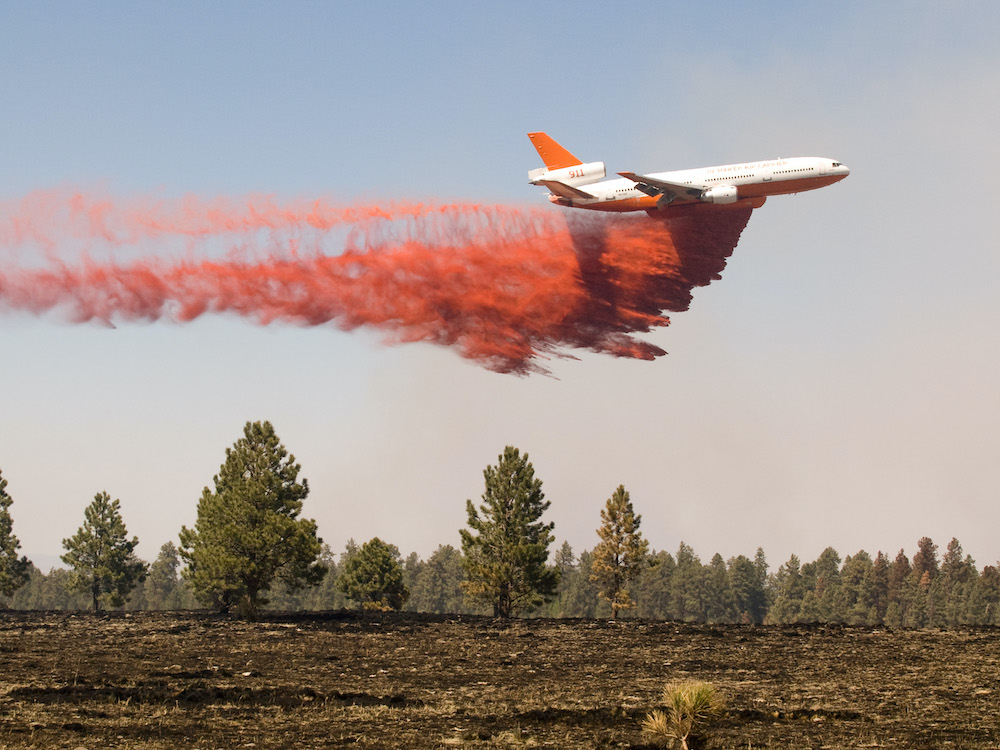
\includegraphics[scale=0.4]{images/dc10.jpg}
  \caption{A DC-10 airtanker, rated for 9,400 gallons, drops retardant
    above Greer, Arizona. Image source: Kari Greer/US Forest Service.}\label{fig:airtanker}
\end{figure}
% TODO: How to cite picture?
% https://www.flickr.com/photos/apachesitgreavesnf/5837741382
% Also appears at https://www.nifc.gov/resources/aircraft/airtankers

\begin{figure}
  \centering
  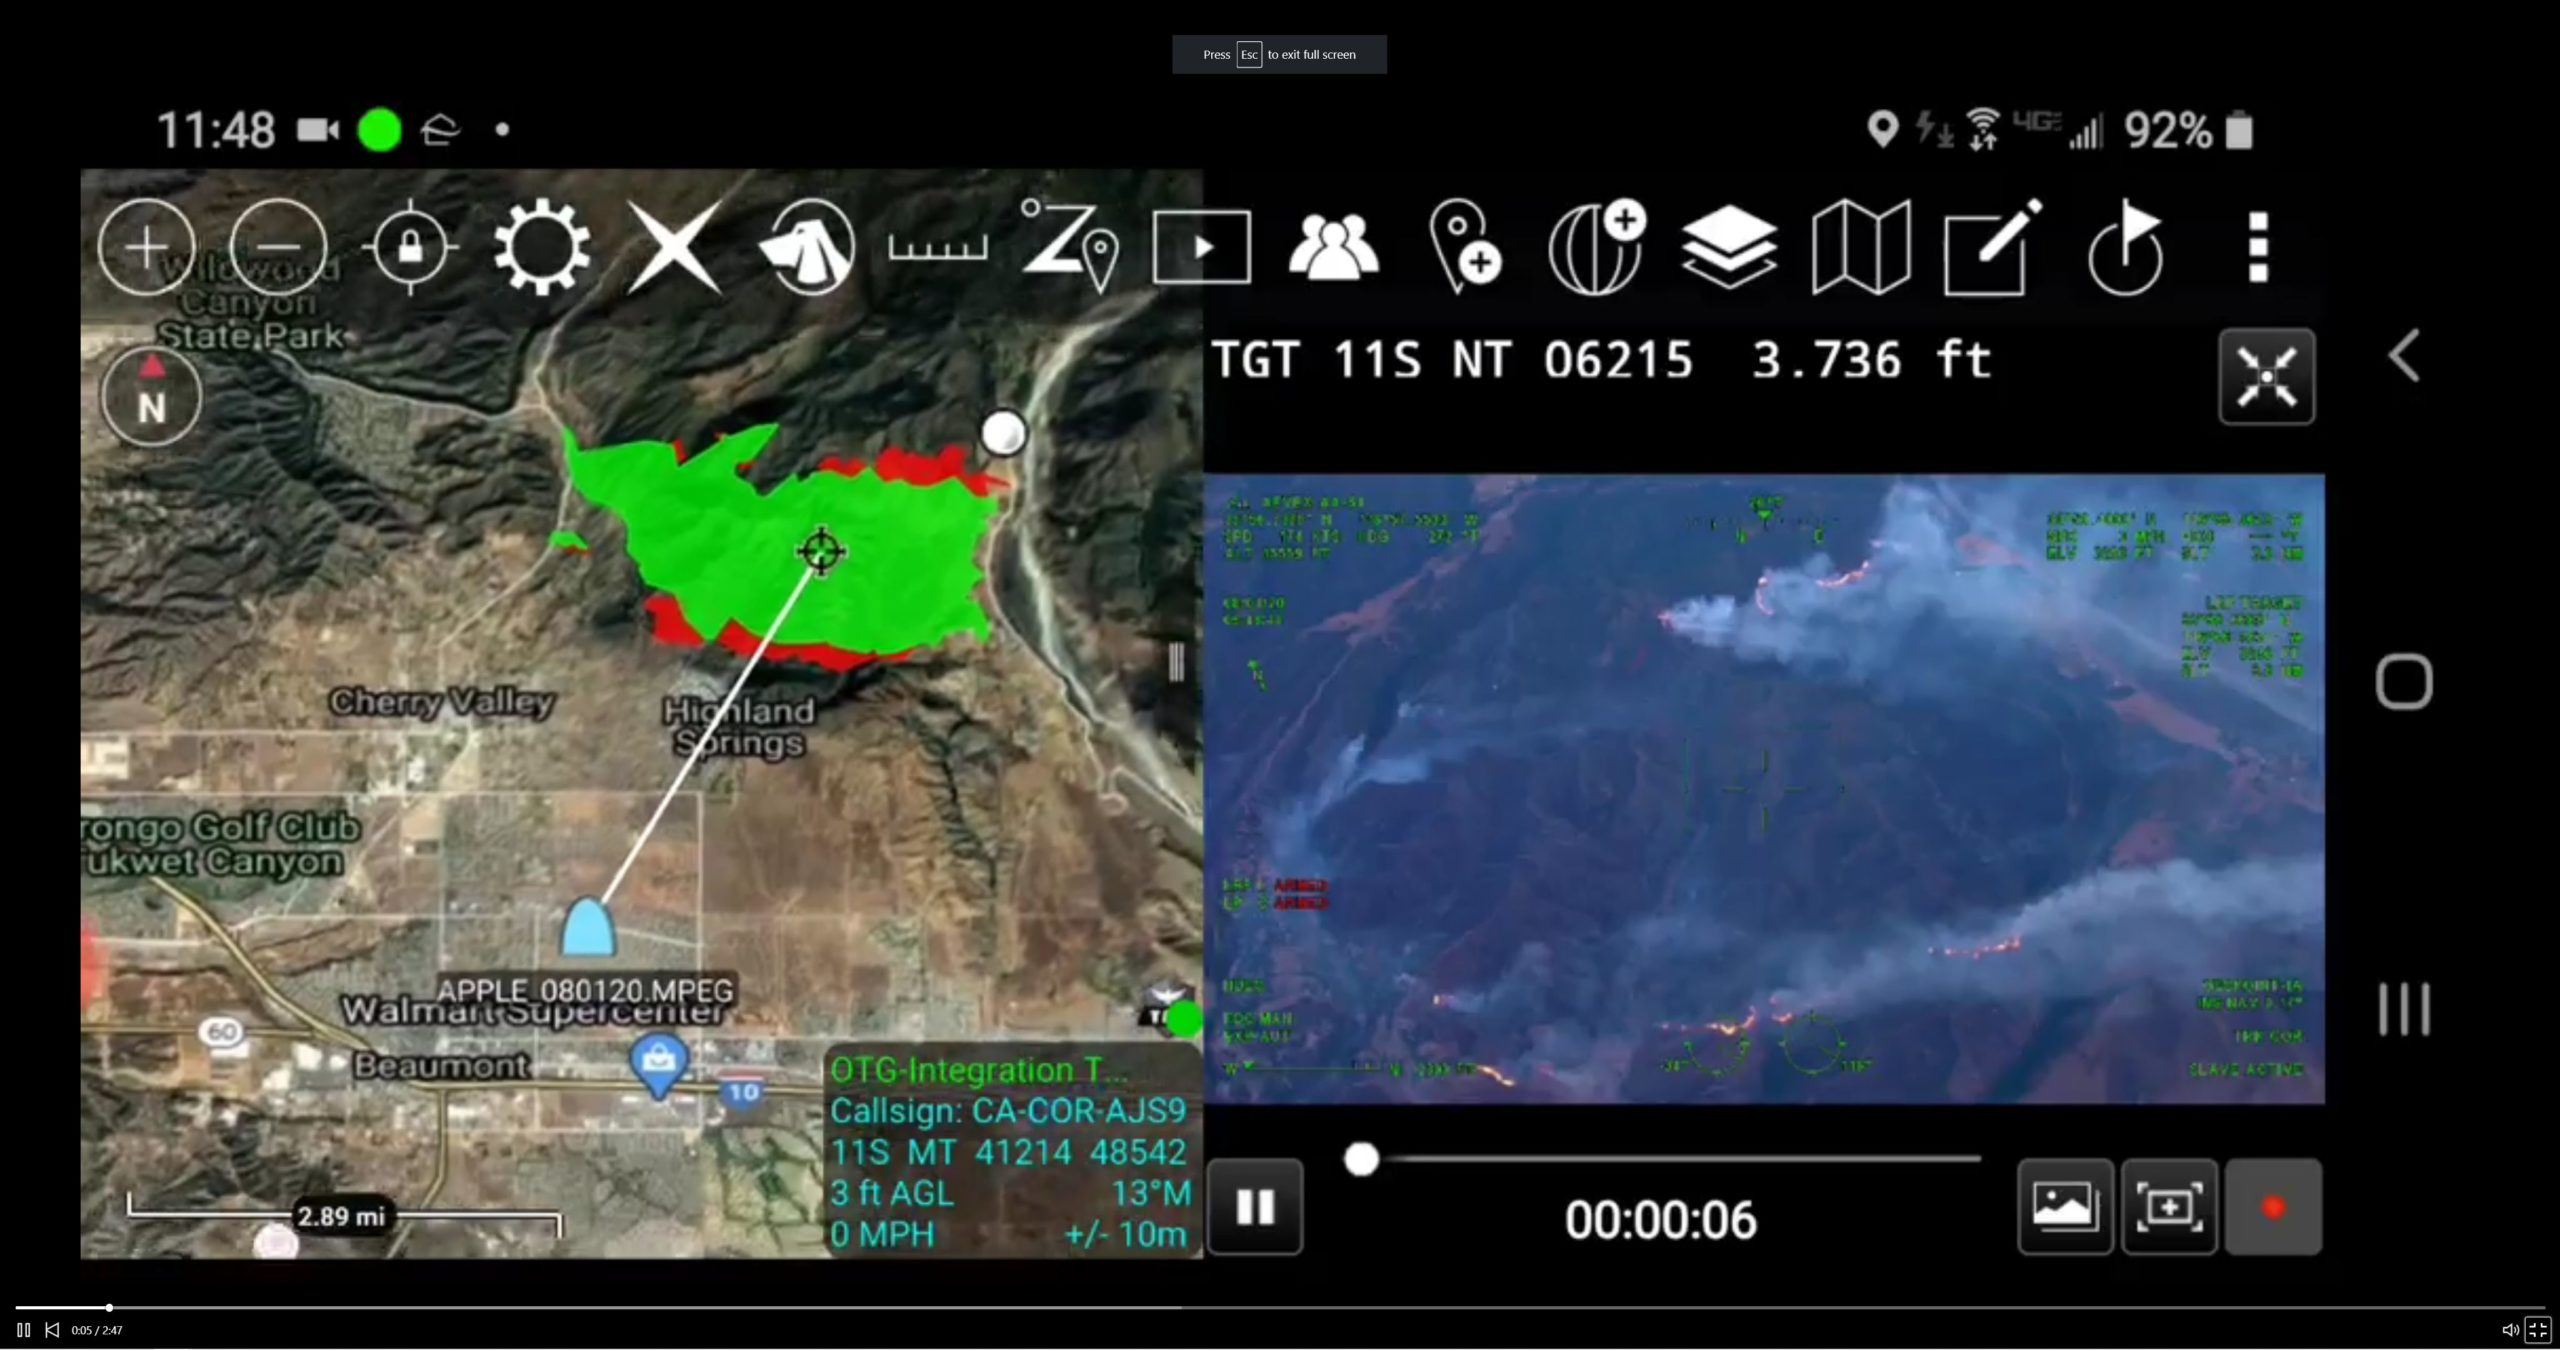
\includegraphics[scale=0.15]{images/forestfire-videox-scaled.jpg}
  \caption{Screenshot of a firefighter using ATAK, where the left
    panel shows a map and the right is a video stream from an air
    vehicle. Image source: Andreas ``AJ'' Johansson}\label{fig:atak}
\end{figure}
% TODO: How to cite picture?
%https://www.civtak.org/2020/08/04/tak-used-in-ca-firefighting-w-aircraft-video/

For example, consider the use of firefighting airtankers, particularly
Very Large Airtankers (VLATs), which can carry over 8,000 gallons of
water or fire retardant \cite{2019:airtankerops}
(Figure \ref{fig:airtanker}). The largest VLATs can drop more than
20,000 gallons---about 170,000 pounds' worth---in a single pass. In
the U.S., these drops are typically made from just 250 feet above the
tree canopy \cite{2019:airtankerops}, and sometimes lower in
practice. This sort of maneuver can easily crush a ground vehicle
\cite{2019:stickney}. In 2018, a firefighter was killed, and three
others were injured, when an unexpectedly powerful drop from a Boeing
747-400 Supertanker knocked down an 87-foot Douglas Fir tree
\cite{2018:calfire}.

Improving firefighter communications can be expected to lead to better
safety outcomes. One such improvement is the through the use of
applications like ATAK---the Android Team Awareness Kit, developed by
the U.S. military in 2010 and later released in a civilian
version. Wildland firefighters are increasingly using ATAK, extended
with aftermarket plugins, on ordinary cell phones to coordinate their
activities in the field (Figure \ref{fig:atak}). A key application of
this tool could be tracking the real-time GPS coordinates of
firefighters for safety monitoring.

Given the risks of VLAT drops, a seemingly reasonable safety measure
might be to disallow drops unless a VLAT's computers have up-to-date
information about the location of ground personnel. Unfortunately,
system-wide safety is not so easily achieved, as the proposed measure
is precisely the sort of thing subject to the safety/liveness
tradeoff. Here, it is important to recognize a linguistic nuance: in
the context of distributed systems, ``safety'' refers to a specific
type of system property; the concept in not inherently related to the
safety of people. A \emph{safety} property is a prohibition that stops
a system from taking an action that might be ``bad'' in some way. Here
is an exemplary safety property for the example above:
\begin{quote}
  $\Psafe$: Ground agents are known to be at least
  100 feet outside the drop zone, and this information is current to
  within 30 seconds, or airtankers will not perform a drop.
\end{quote}
By contrast, a \emph{liveness} property demands some kind of action
from a system, usually one that is ``good'' in some way. A
characteristic of liveness properties is that they place an upper
bound on the allowable delay of something. An exemplary liveness
property for our scenario might be the following:
\begin{quote}
  $\Plive$: A VLAT on the ground will take off and
  perform a drop within 20 minutes of receiving a request from an
  incident commander. \footnote{The Chief of Flight Operations for Cal
    Fire cited 20 minutes as an upper bound on the response time for
    aerial firefighting units within designated responsibility areas
    in an interview with PBS \cite{2021:aerialfirefighting}.}
\end{quote} Note that $\Plive$
is a liveness property, not a safety property in the narrow technical
sense, but it impacts human safety: it might be critical for VLATs to
perform drops quickly if a wildfire is threatening the safety of
ground personnel.

Safety and liveness are frequently dual mandates that cannot be
guaranteed simultaneously. Such is the case in our example: though
$\Psafe$ and $\Plive$ are both
desirable, certain situations will force policymakers to prefer one
over the other. Consider the fact that the wildland firefighting
environment is frequently GPS-denied: heavy smoke, multipath effects,
and so on can easily prevent a consumer-grade cellphone from obtaining
reliable GPS coordinates. Additionally, factors like a damaged radio
tower or environmental obstructions like a tall mountain can prevent
communications between the air and ground. Such conditions would
prevent a VLAT's computers from knowing the locations of ground
agents, which immediately presents a dilemma: should the crew proceed
without knowing the locations of ground personnel, maintaining
$\Plive$ at the cost of $\Psafe$,
or should it be cautious and wait for more information, maintaining
$\Psafe$ at the cost of $\Plive$?
There is no simple answer, with either choice presenting a downside
with respect to the broader goal of system-wide safety.

Besides the safety/liveness tradeoff, the previous example exhibits
two other themes important in distributed systems, both of which will
be explored further in this document. The first is the
\emph{epistomological} nature---concerned with what information is
\emph{known} by \emph{whom}---of reasoning about distributed
systems. This aspect is reflected in wording of
$\Psafe$ in VLAT example: Ground agents are known
(by the VLAT's computers) to be outside of a dangerous area. This
situation requires a deeper and more sophisticated analysis than one
simply considering what is true, but not necessarily
known. Mathematically, the logic of distributed agents is not the
ordinary propositional logic but the modal logic S5, which extends
propositional logic with additional axioms governing
knowledge.\footnote{The application of S5 to reason about distributed
  systems is the topic of \cite{kshemkalyani_singhal_2008}, Chapter
  8.} Distributing knowledge requires communication between agents
over a period of time over the network, which is not instantaneous and
reliable, and it is from these imperfections that the safety/liveness
tradeoff arises.

The second aspect exhibited above, albeit negatively, is that of
\emph{continuity}. A continuous system can flexibly adopt to its
environment, but a discontinuous system is rigid and may exhibit
suddenly different behavior in response to only small changes in the
environment. The properties $\Psafe$ and
$\Plive$ exhibit a stark lack of continuity because
they are inflexible, all-or-nothing propositions. Suppose that agents
are known to be $500$ feet outside the drop zone, but the information
is only current to within 31 seconds---this extra second technically
violates $\Psafe$, though it should be inferrable
that the ground agents are well away from danger. In particular, this
example highlights that system-wide safety is more of a quantitative
concept than a Boolean (true-or-false) one. A distributed system in a
network-challenged environment should exhibit smoothly varying
properties in response to its inputs, and ideally allow ``tuning'' the
system's properties for the particulars of its environment at any
moment. The technical aspects of this theme are the focus of Section
\ref{sec:continuous-consistency}.

\subsection{Communication Patterns in the Field}
\label{ssec:communication-patterns}
We now consider some of the communication patterns that occur in
wildland firefighting. Readers may be surprised to learn that the
state of the art is somewhat primitive, largely due to the sparse
permanent communications infrastructure that exists in this
setting. This makes wildfires an interesting and generalizable example
for other kinds of civil disaster environments where the network is
unreliable.

One important concept to draw attention to is a kind of ``geospatial
locality of reference'' that system designers should consider. By
this, we mean the concomitance of two observations which, while not
guaranteed rules, are approximately true in many circumstances. The
first observation states that nearby agents have aligned interests:
\begin{quote}
  $\textbf{O}_1$: Agents with the most urgent need to coordinate their
  actions will usually be located closer together and require similar
  kinds of information.
\end{quote}
The second observation states that nearby agents have more reliable
communications:
\begin{quote}
  $\textbf{O}_2$: Agents that are located closer together generally
  enjoy more reliable communications between them than agents that are
  far apart. Conversely, information that travels long distances tends to
  be delayed or degrade in quality.
\end{quote}

These related observations are what is meant by simply the
``locality'' principle. Locality is a crucial factor to analyze
because, as presented in Section \ref{sec:background}, there are major
theoretical and practical limits to how well agents can coordinate
\emph{globally}, meaning with all agents knowing and agreeing on
everything. To the extent the system exhibits locality, coordination
can be achieved using more efficient short-range communication than
less efficient long-range communication. Here, ``efficient'' should be
read broadly, measured with respect to things like battery life,
message delay, reliability, cost-effectiveness, equipment weight, and
so on. This raises the question of how to most efficiently utilize
network resources to achieve adequate levels of consistency. This
question is revisited in Section \ref{sec:continuous-consistency}.

\subsubsection{Communication on the Ground}
\label{sssec:ground-communication}
In the field, communication between firefighters and other agents is
often facilitated by handheld (analog) land-mobile radio (LMR). These
radios are inherently limited in their battery life, bandwidth,
effective range, and ability to work around environmental factors like
foliage and smoke.

As an alternative to using a radio, it is common for wildland
firefighters in the field simply to shout commands and notifications
to nearby personnel. This exhibits the locality principle: a
substantial amount of communication occurs directly between nearby
firefighters working on closely related tasks that can communicate
without network infrastructure. In a future environment where agents
might be equipped with body-worn sensors and or even some form of
heads-up display (HUD), this sort of low-range local communication
might be facilitated by relatively inexpensive, low-power technologies
such as Bluetooth, without the need for more sophisticated (and heavy)
equipment.

Communication over a long distance requires infrastructural support,
such as the use of cell towers and repeater stations. Typically,
disaster response environments have scarce permanent infrastructure:
in a wildland fire setting, perhaps a few repeaters mounted to a
nearby watch tower. Ad-hoc infrastructure, such as Cells On Wheels
(COWs) or Cells on Light Trucks (COLTs)---i.e. portable cellular
towers---can sometimes be deployed on an as-needed basis if the
location allows for it. Similar kinds of equipment can also be mounted
to backpacks and carried into the field by specially-trained users. A
common issue is making sure that all equipment is properly configured,
for instance that radios are listening on the correct
frequencies. Configuration is especially critical when different
agencies and groups need to interoperate---another problem highlighted
during the September $11^\textrm{th}$ attacks.

\begin{figure}[t]
  \centering
  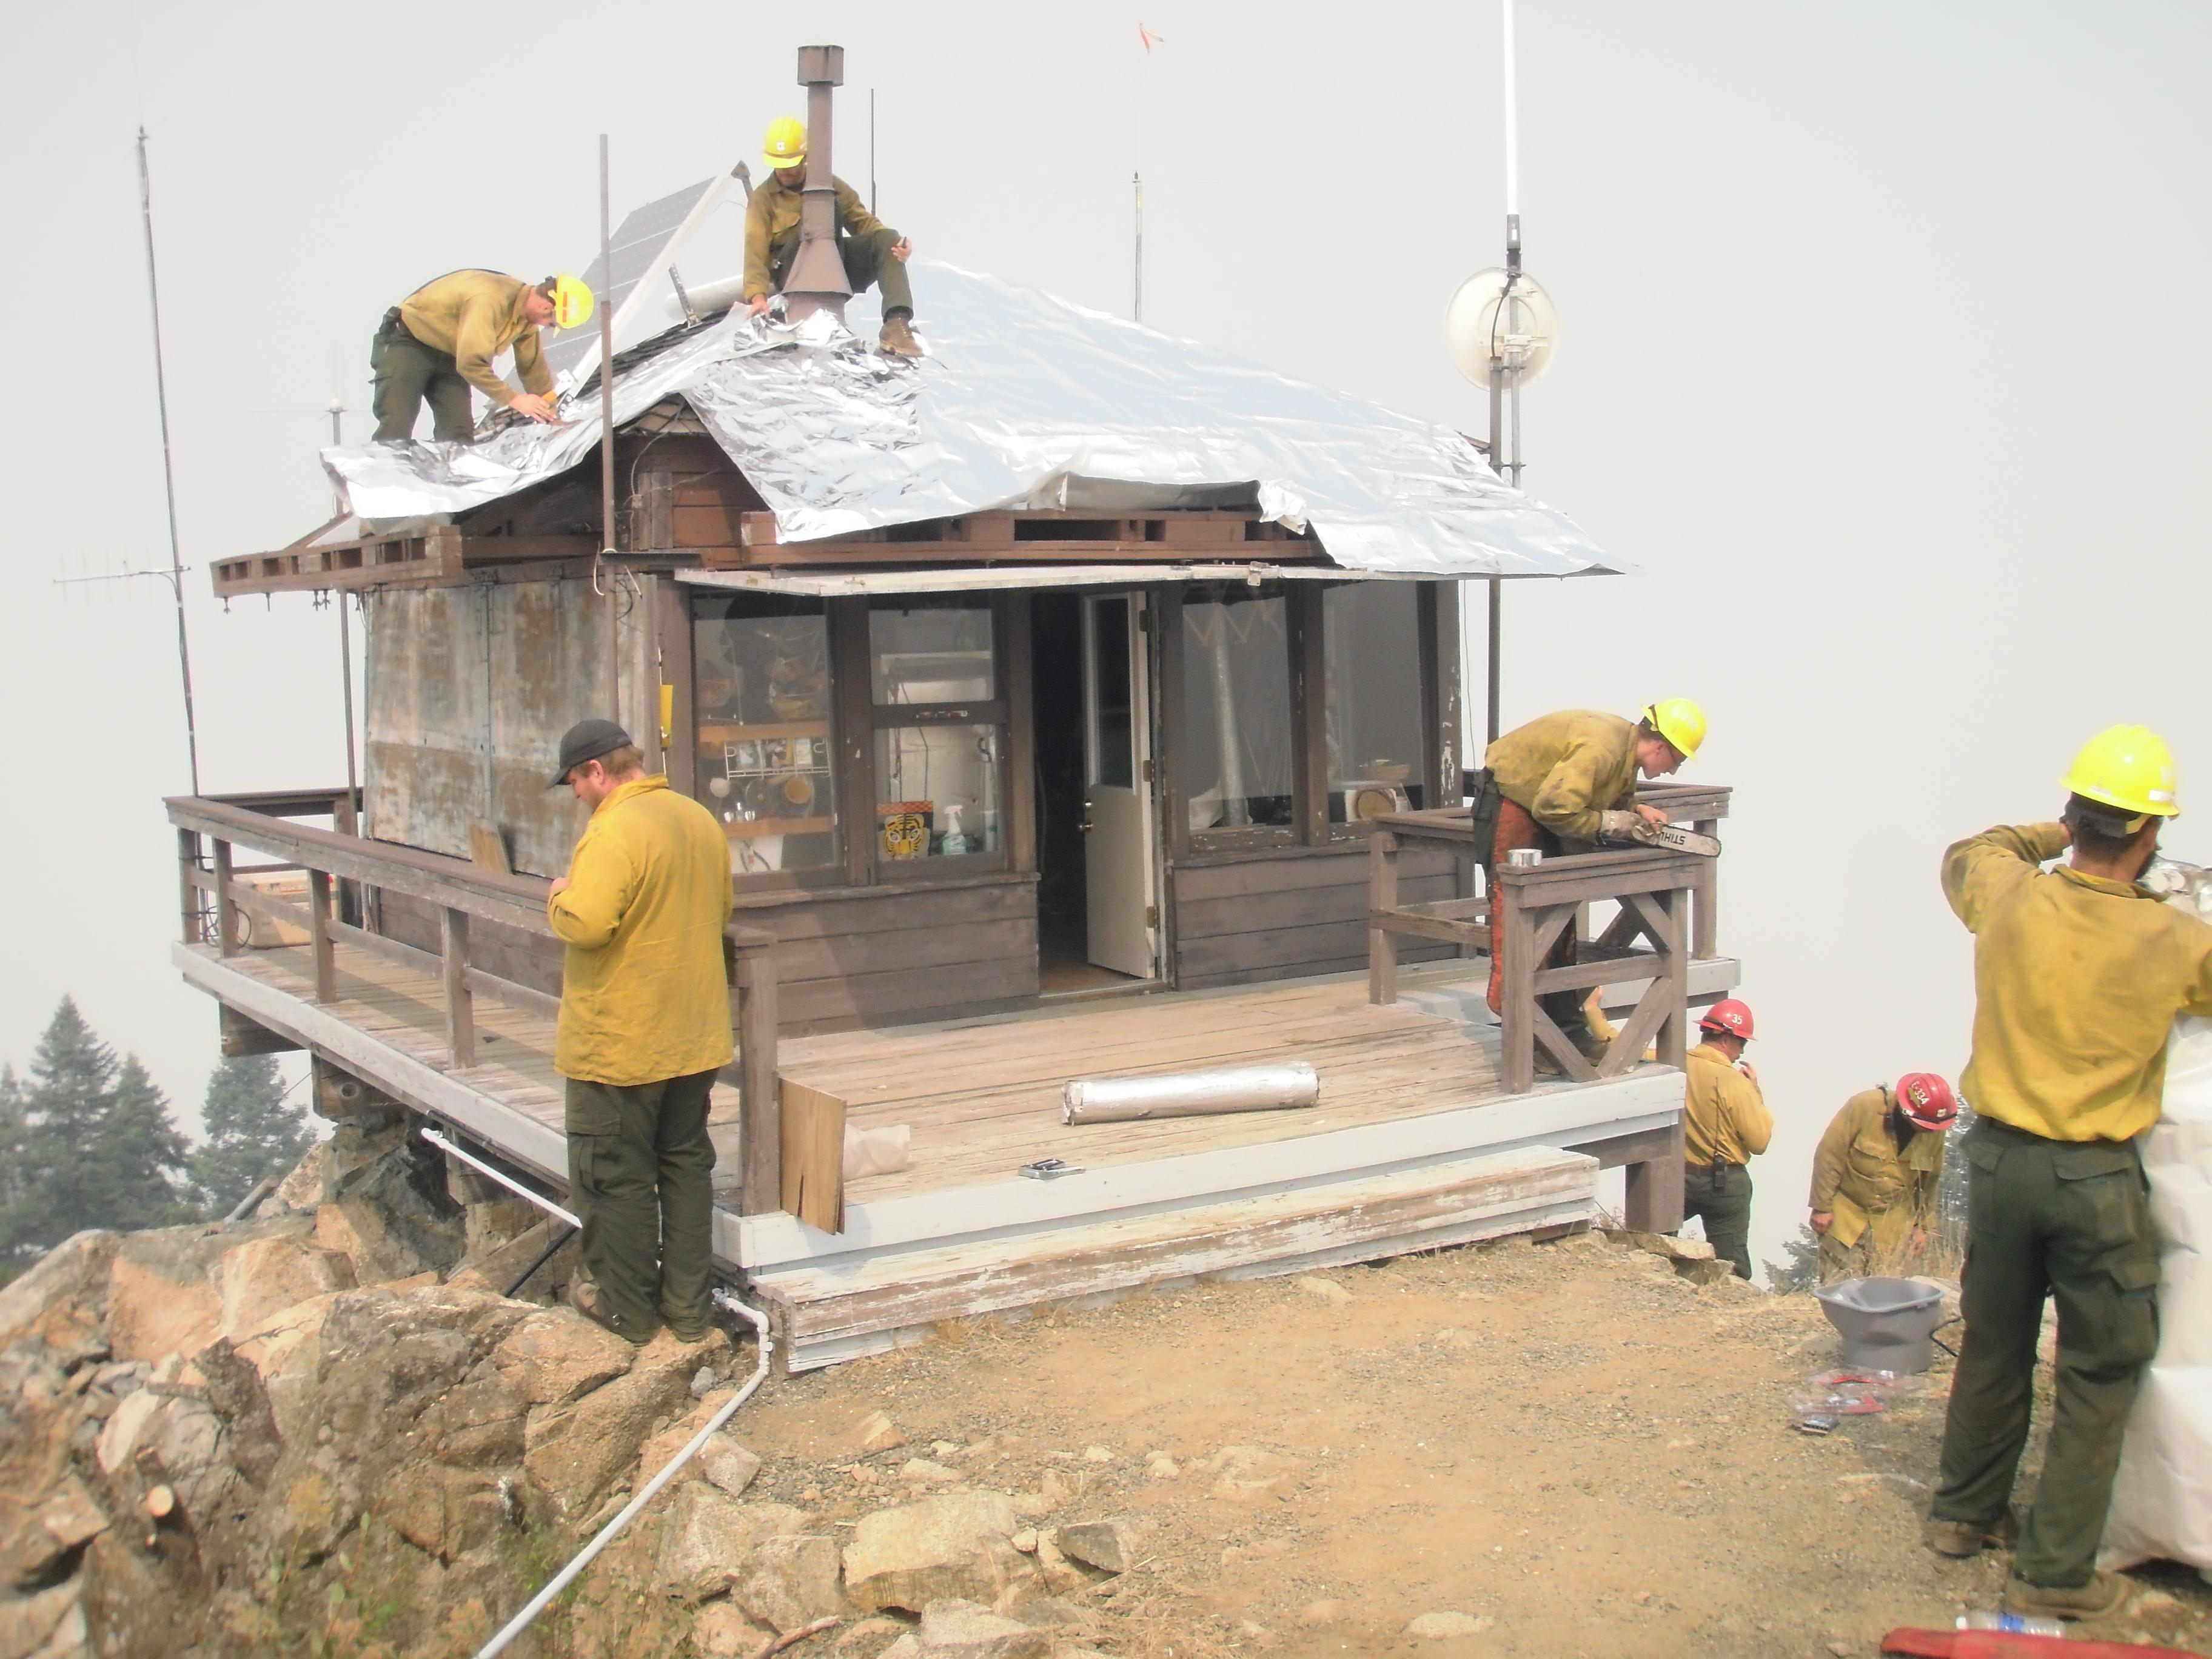
\includegraphics[scale=0.085]{images/ironside.jpg}
  \caption{The Ironside Mountain lookout and radio repeater station,
    shown here with protective foil on August $10^\textrm{th}$, 2015
    during the 2015 River Complex fire. This particular fire burned
    77,077 acres over 77 days.}
  \label{fig:ironside}
\end{figure}
% TODO: How to cite picture?
%https://web.archive.org/web/20150923190323/http://inciweb.nwcg.gov/incident/photograph/4431/44/45122/

Use of centralized infrastructure comes with the potential for
widespread failure when the infrastructure breaks down. For example,
in California, the Ironside Mountain lookout/repeater station (seen in
Figure \ref{fig:ironside}) was destroyed during the 2021 Monument
Fire, which burned approximately 223,124 acres over 88 days
\cite{2021:monumentfire}. The Ironside Mountain station had strategic
importance, being located on a tall ridge. According to a video blog
from a volunteer firefighter involved in the incident, its loss
prevented communication between operators on different sides of the
ridge, in networking parlance creating a \emph{partition} that lasted
until crews could ascend the ridge to deploy a temporary station:
\begin{quote}
  ``When {[}the Ironside Mountain lookout station{]} burned down the
  radio repeater went with it. And so communications were lost across
  the fire\ldots{} one side of the fire couldn't talk to the other
  side\ldots.  So it was kind of a critical job to get that road
  cleared so that the radio crews could go back up there and set up a
  temporary radio tower.'' \cite{2022:mechfire}% See also https://web.archive.org/web/20220809061927/https://www.youtube.com/watch?v=4F2dDKMgAME
\end{quote}
A scenario where communication between two groups is completely
severed is exactly the sort of thing considered by the CAP theorem in
Section \ref{sec:background}.

\paragraph{Ground vehicles}
Large numbers of ground vehicles---sometimes on the order of 100
during a major response---are involved in wildfire
suppression. Besides various types of firetrucks, bulldozers and
similar vehicles are commonly used to control the landscape and
perimeter of the fire. An advantage of vehicles is that they can carry
heavier and higher-power communications equipment than a human. For
instance, a vehicle could be equipped with a BGAN or VSAT satellite
terminal to maintain a high-bandwidth connection back to a central
location. Additionally equipping the vehicle with something like a
Wi-Fi or cellular base station using the satellite connection as
backhaul would let the vehicle act as a bridge between agents in the
field and central coordinators such as incident commanders or 911
dispatchers.

\subsubsection{Communication in the Air}
Wildland firefighting increasingly involves the use of helicopters and
fixed wing aircraft. Civil aviation has traditionally employed simpler
communication patterns than this use case demands. For instance,
aircraft equipped with Automatic Dependent Surveillance-Broadcast
(ADS-B) monitor their location using GPS and periodically broadcast
this information to air traffic controllers and nearby aircraft. This
sort of scheme has worked well in traditional applications, where
pilots typically only monitor the general locations of a few nearby
aircraft. The locality principle is exhibited here, too: aircraft have
the highest need to coordinate when they are physically close and
therefore in range of each other's ADS-B broadcasts.

In our setting, a large number or aircraft, easily on the order of 10 or
more, may need to operate in a small area, near complex terrain,
during adverse conditions, often at low altitude. In other words, the
demands are many and the margins for error are small. This sort of use
case calls for more sophisticated coordination schemes between
airborne and ground-based elements than solutions like ADS-B provide
by themselves.

As aircraft generally have better line-of-site to ground crews than
ground crews have to each other, firefighters sometimes relay messages
to air-based units over the radio, which in turn is relayed back down
to other ground units. The locality principle comes into play for this
sort of message relaying scheme, but in the negative direction:
relaying allows knowledge to travel farther but requires more resources and effort,
and the extended reach comes at the cost of introducing delays and
possible degradation of message quality, as in the classic game of
``telephone.'' Hence, this mode of communication has generally been reserved for
more critical information.

The Communications Program of the Civil Air Patrol (a civilian
auxiliary of the U.S. Air Force) is sometimes deployed to provide
communications for firefighters on the ground using airplane-mounted
radio repeaters. Air-based repeaters are better than the ``telephone''
scheme in the previous paragraph as they do not require as much human
intervention to receive and re-transmit information. That is, this
form of relaying is more \emph{transparent}. In this future, this sort
of service could be provided autonomously by portable infrastructure
futuremounted to unmanned aerial vehicles (UAVs), which might perform
additional functions such as tracking the fire perimeter.

In future environments, we envision resilient networks formed from
heterogeneous collections of smaller networks, incorporating various
communication technologies such as digital radios, Wi-Fi, 4G/LTE, and
satellite communications. Communications in the field may incorporate
aspects of mesh networks and mobile ad-hoc networks (MANETs). The
infrastructure will be comprised of both permanent infrastructure and
temporary equipment carried into the field by responders, vehicles on
the ground or in the air. Given the environmental challenges, we
assume that two agents will often only have intermittent end-to-end
connectivity, if any. Facilitating communication through such a
dynamic and chaotic mobile network calls for a disruption-tolerant
networking (DTN) architecture, which provides a custody transfer and
store-carry-forward model that is resilient to disruption
\cite{2021:intro-dtn}. The exact form of such a network remains an
open question for future investigation.

\subsection{Data Collection and Processing}
\label{ssec:data-collection}
Perhaps the most universally acknowledged expectation for future
disaster response environments is a heavy reliance on data
gathered from both humans and sensors. Besides improvements to
communications that facilitate information sharing, we expect advances
in machine intelligence to greatly influence how this data is
handled.

Agents in disaster response environments will be both producers and
consumers of data, and this data will need to processed by humans and
machines in ways that agents can readily make sense of to support
their decision-making. Just some of the possible sources and types of
pertinent data are as follows:
\begin{itemize}
\item Free-form communication, especially real-time or recorded voice messages
  broadcast to many agents at once, which may need to be processed by
  machines to extract the most pertinent information into a more
  actionable format
\item The exact or estimated location of victims, firefighters,
  vehicles, hazards, and so on displayed on applications like ATAK
\item Medical information gathered from victims, perhaps stored in and
  collected from electronic triage tags \cite{2009:triagetag}
\item Data about current and predicted fire behavior gathered from
  systems like the Fire Integrated Real-time Intelligence System
  (FIRIS) or NASA's Fire Information for Resource Management System
  (FIRMS)
\item Weather data from the National Weather Service
\item Topographic information about the terrain, highlighting for
  instance the location of rivers and roads that could form a fire
  control line
\item Planned escape routes, rendezvous points, safety zones, and
  landing zones
\item Availability and dispatching of assets, e.g.~ambulances,
  airtankers, or crews on standby, such as the prototype application
  considered by Monares et al. \cite{2011:monares}
\end{itemize}
In a perfect environment, such information would be shared with all
necessary agents in whole and instantly. In reality, agents will be
presented with information that is sometimes incomplete, out of date,
or contradictory---all problems that are further exacerbated by an
unreliable network. A competing concern is that the information
presented will be \emph{overcomplete}, filled with petty details that
distract agents from their important tasks.

In some ways, future systems for disaster response will bear
resemblence to future systems for warfighting, such as the conceptual
\emph{Internet of Battle Things} (IoBT) \cite{2016:iobt}. To quote
from that paper, agents ``under extreme cognitive and physical
stress'' will be subject to a highly dynamic and dangerous
environment. Various kinds of technology will assist humans by
providing data to support sensemaking, but a contraindicating concern
will be flooding agents with a ``massive, complex, confusing, and
potentially deceptive ocean of information.'' To avoid ``swimming in
sensors and drowning in data'' \cite{2010:magnuson}:
\begin{quote}
``Humans seek well-formed, reasonably-sized, essential information
  that is highly relevant to their cognitive needs, such as effective
  indications and warnings that pertain to their current situation and
  mission.'' \cite{2016:iobt}
\end{quote}

We propose that researchers in field of Human-Computer Interaction
(HCI) should take up the question of how public safety agents under
stress can process and respond to the flood of information they may
face as public safety systems become more complex. HCI has been
defined as follows:
\begin{quote}
  ``A subfield within computer science concerned with the study of the
  interaction between people (users) and computers and the design,
  evaluation and implementation of user interfaces for computer
  systems that are receptive to the user's needs and habits.'' \cite{2009:hci-definition}
\end{quote}
HCI research offers insights into how interfaces should be structured
to avoid cognitive overload and facilitate intuitive control without
distracting users. As emergency control becomes increasingly
data-driven, particularly in centralized hubs like dispatch centers
that aggregate diverse streams of information, the challenge of
ensuring that users can interact effectively with these systems will
become increasingly important.

\subsubsection{Adversarial Behavior}
One feature of the Internet of Battle Things worth highlighting is
``the adversarial nature of the environment.'' This feature is common
also to disaster environments, whether resulting incidentally from
``fog of war'' effects or deliberately caused by malicious actors
seeking to exploit a civil disaster. Section
\ref{ssec:communication-patterns} cited a real-world example of a
critical communications station destroyed by wildfire, perhaps
comparable to an attack by enemy forces.

There is a growing trend in disaster response to rely on
``crowdsourced'' information, where public safety officials process
reports from the general public over non-traditional channels like
social media. However, a significant vulnerability of crowdsourcing
information is the potential for confusing of contradictory reports,
which can resemble intentional deception. Rumors frequently plague
disaster relief environments, which are quite susceptible to
misinformation. For instance, during Hurricane Harvey in 2017, there
were unconfirmed rumors of shots being fired at volunteer rescuers
\cite{2017:cajun-navy-rumors}. Tracing reports back to their source is
often difficult. Even fully malicious activity like
``swatting''---placing a fake 911 call to cause a large police
response---is often observed in public safety. Whether misinformation
is spread with malicious intent or through well-meaning confusion, the
proliferation of false information in this chaotic environment can
have adversarial effects. This should be anticipated as part of a
careful approach to modernizing systems in this space.

\subsubsection{Allocation of Network Resources}
\label{sssec:allocation-of-network-resource}
Communications in disaster response environments might even be less
reliable than in the battlefield (setting aside offensive behavior
like signal jamming), requiring a greater emphasis on the preservation
of scarce network resources. For instance, a group of volunteer
firefighters would have fewer resources than a tactical military unit,
relying on commercial off-the-shelf (COTS) equipment rather than best
in class hardware like sophisticated handheld satellite links. High
bandwidth channels will often be in short supply, while adverse
conditions like inclement weather are assumed.

Given the heavy reliance on data and the scarcity of reliable
communication channels, we expect a complex interaction between the
high-level needs of distributed applications (e.g. an application for
sharing real time weather data) and low-level concerns about network
resources. This is because only the applications have enough
information to determine which data is the most important and must be
shared with whom first, while only the network-level protocols have
enough information and control to make prudent use of scarce network
availability.

There is a widely accepted wisdom in computing---the end-to-end
principle \cite{1984:end-to-end}---which suggests roughly that
applications should not make assumptions about the network, and that
the network should be relatively agnostic to high-level application
logic. However, in natural disaster environments where resources are
scarce and reliable communication is critical, these subsystems may
need to be more tightly integrated in how they influence each other to
achieve the best performance. This approach would not contravene the
end-to-end principle, but would involve carefully considering its
application in this relatively extreme context.

Consider, say 5 to 10 years in the future, a centralized data fusion
application that running in an edge data center.\footnote{An
  \emph{edge} data center is one located closer to a network's edge,
  nearer to users, to provide low-latency communications for
  time-sensitive applications. Edge centers support applications that
  require significant amounts of information processing---enough that
  the application must be hosted in a datacenter, where compute
  resources can be scaled dynamically, rather than colocated with
  users where resources are limited.} This application could detect
critical events like a fire crossing a control line (a phenomenon
called \emph{slopover}) and alert ground responders. It might also
warn responders who have strayed too far from an escape route or
safety zone. These are high-priority notifications, so it would be
worthwhile to allocate scarce network resources to convey them to the
relevant parties in real-time.

On the other hand, while it may be beneficial for each firefighter to
have real-time information about the location of every other
firefighter, this may not always be critical. If transmitting this
data strains the network, then perhaps only the general location of
other crews or nearby teams should be sent. If the network is
extremely constrained, communication may be restricted to only
information strictly relevant to preserving life to ensure this is
delivered swiftly and reliably. Thus, network allocation is a dynamic
calculation influenced both by the criticality of the information
(which is determined by the application logic) and the availability of
network resources at a particular location. Advanced systems should
provide mechanisms like Quality of Service (QoS) values to allow
prioritizing certain communication. Such mechanisms can be
incorporated into a control loop where applications generate feedback
that drives the decision-making process in lower-level parts of the
network. However, traditional QoS mechanisms may not be enough---even
the routing protocol of the network may need to be more specialized to
higher-level applications than in traditional environments.


\section{Introduction to Distributed Systems}
\label{sec:background}
In this section, we distill two core topics in the theory of
distributed systems: causality and timekeeping, along with shared
memory consistency.  Our discussion is primarily informed by the
manuscripts of Coulouris et al.  \cite{coulouris2005distributed} and
Kshemkalyani and Singhal \cite{kshemkalyani_singhal_2008}. We focus on
building applications relevant to the scenarios described in Section
\ref{sec:disaster-response}, aiming to highlight obstacles and
strategies for developing distributed systems that can endure the
delays and disruptions inherent to these communication-challenged
environments. Readers wishing for a condensed summary of the main
highlights may skip to Section \label{ssec:background-summary}.

At its core, a distributed system is a network of independent entities
working together to solve problems too complex for any one part to
tackle alone. From a bird’s-eye view, the systems we envision are
intricate and complex, made up of diverse, interconnected elements:
field agents like firefighters, their handheld devices, airborne and
ground vehicles loaded with communication and computing tools, swarms
of sensors and IoT devices, and so on. These decentralized components
operate alongside more centralized hubs: data fusion centers, incident
commanders, public safety answering points (PSAPs), and emergency
operations centers (EOCs). We imagine these components being woven
together by a patchwork of communication technologies ranging from
analog and digital radios to Bluetooth, Wi-Fi, LTE, 5G, satellite
communications, and ad-hoc mesh networks like
Meshtastic\footnote{The website of the
  Meshtastic project describes it as an ``open source, off-grid,
  decentralized, mesh network built to run on affordable, low-power
  devices''. See \url{https://meshtastic.org} or
  \url{https://github.com/meshtastic}.}, DECT-2020
NR\footnote{DECT-2020 NR, also called NR$^{+}$, is a non-cellular 5G
  standard intended for Internetof Things (IoT) operations. For a
  technical discussion see \cite{2022:dect-2020-nr}.}, and
others. Together, the systems form a dynamic mosaic of elements
cooperating to save lives and protect proprty.

Given the unpredictable nature of the environment and the locality
principle outlined in Section \ref{sec:disaster-response},
communication between edge components---such as field operators---and
centralized hubs is often inconsistent, sometimes available only
intermittently. As a result, information flow is subject to
appreciable delays compared to the timescale of critical events like a
fire shifting direction or a dangerous condition being detected. In
other words, the computing landscape is unmistakably
\emph{distributed}. Singhal and Shivaratri \cite{10.5555/562065}
define a distributed computing system as:
\begin{quote}
  ``A collection of computers that do not share common
  memory or a common physical clock, that communicate by message
  passing over a communication network, and where each computer has
  its own memory and runs its own operating system.''
\end{quote}
This stands in contrast to a centralized computing environment, where
processes can seamlessly share data through common memory, and memory
access times are considered negligible.

For our use cases, message-passing latencies are not only significant
but unpredictable and difficult to control. As a result, we can safely
assume that some parts of the wider system will not have
instantaneous, complete knowledge of every new piece of
information. Only a few components, if any, will be able to maintain a
global systemwide awareness. While deploying additional network
resources in the field—such as COWs (Cells on Wheels) and COLTs (Cells
on Light Trucks)—can help, the inherently distributed nature of the
environment cannot be fully overcome or abstracted away. This reality
must be embedded in the design of the software and networking
architecture itself. Typically, this manifests in a shared
``middleware'' layer to coordinate the numerous moving parts, ensuring
they function as a unified system.

The fragmented flow of information presents several challenges for
system designers. Foundationally, one of the primary computer science
problems is that unpredictable latencies make it difficult for
components to maintain a common understanding about the global
sequence of events. For similar reasons, it becomes challenging for
processes to synchronize and agree on shared values, such as the
current number of firetrucks available for dispatch. The remainder of
this section will delve into these issues with more technical depth,
while later sections will examine how some of these challenges can be
reflected in the middleware design.

\subsection{Physical Synchrony}
\label{ssec:physical-synchrony}
A lot of challenges in distributed computing could be
straightforwardly overcome if we assume that all participants have
instantaneous access to a common time base, i.e.  synchronized
clocks. Let us explore why fine-grained synchronization is not a
tenable assumption, at least not for all purposes.

Physical clocks, especially consumer-grade ones, suffer from
\emph{drift}, which is to say they do not all run at the same
rate. Experienced IT administrators will testify that clocks can also
be prone to misconfiguration. An incorrect date, time, timezone, or
daylight saving time policy setting is a common source of IT issues,
typically causing time-based security mechanisms like TLS
authentication to misbehave. Consider also that devices may spend a
long time sitting unpowered in storage without maintaining an
always-on clock. For these sorts of reasons, we would not want to rest
the integrity of a safety-related system on the assumption that a
numerous and diverse assortment of devices have precisely synchronized
internal clocks.

Clock drift can be corrected for using, for instance, signals from GPS
satellites, but as mentioned in Section \ref{sec:disaster-response},
civil disaster environments are frequently GPS-denied: factors like
mountainous terrain, heavy smoke, and subterranean operations can lead
to errors or block signals entirely. Protocols like the Network Time
Protocol (NTP) \cite{rfc1119} work to bring clocks into
synchronization with respect to an authoritative source. On the public
internet, NTP typically achieves synchrony to within values on the
order of tens of milliseconds \cite{rfc1128}, but it is not clear the
level of synchrony that can be expected from NTP in the sorts of use
cases we have in mind. A field device initialized without internet
access may have no idea what the time is, but it must still operate.

For our use case, what seems most important about time is that
\emph{the future cannot influence the past}
\cite{1989mattern}. Fortunately, this sort of invariant can be
enforced with mechanisms that do not rely on measuring real
time. Below, we explain how so-called logical clocks can be used to
measure and enforce a key relation between events, this being their
\emph{causal precedence}.


\subsection{Message Passing and Causality}
\label{ssec:message-passing}
We model a distributed system abstractly as a fixed set
$\mathcal{P} = \{P_1, P_2, \ldots P_n\}$ of \emph{processes} which
undergo atomic (indivisible) state changes known as
\emph{events}. Events are divided into three types: internal events,
representing state changes inside a single process, and send and
receive events corresponding to \emph{messages} passed between
processes. Note that this framework is quite abstract and applies to
any kind of packet-based communication technology. To draw out the
core issues surrounding messaging, the diagrams in this section do not
depict any internal events, as they represent state changes that are
not directly viewable to the network or other processes.

Throughout the section, processes and networks are opaque blackboxes,
which concentrates our attention on the ramifications of unpredictable
network latencies. We implicitly assume the reliable asynchronous
network model: when a message is sent between processes, it certainly
arrives at some point in the future, but we cannot say anything about
when or in what order compared to other messages. At times, we
consider the possibility that a message may never arrive. The choice
depends on which networking technology (or which layer of the OSI
networking model \cite{1983:osi-reference-model}) is under
consideration.

Figure \ref{fig:message-latencies} illustrates a series of time
diagrams for messages exchanged between three processes: $P_1$, $P_2$,
and $P_3$. The $x$-axis represents the flow of real time from left to
right, which each process represented by a worldline depicting the
events occurring within that process. Each message, $m$, originates
from a send event $\msend{}$, marking the moment the message is
dispatched across the network by its source process. The delivery of
the message corresponds to a receive event, $\mrecv{}$. For now we
assume messages have a single receiver. We write subscripts on
messages to distinguish them for clarity, but these are not inherent
to the messages themselves.

\begin{figure}[p]
  \setlength\belowcaptionskip{5ex}
  \begin{subfigure}{1\textwidth}
    \centering
    \begin{pgfpicture}
\pgfpathrectangle{\pgfpointorigin}{\pgfqpoint{390.0000bp}{154.0000bp}}
\pgfusepath{use as bounding box}
\begin{pgfscope}
\pgfsetlinewidth{1.0000bp}
\definecolor{sc}{rgb}{0.0000,0.0000,0.0000}
\pgfsetstrokecolor{sc}
\pgfsetmiterjoin
\pgfsetbuttcap
\pgfpathqmoveto{277.3427bp}{75.5915bp}
\pgfpathqlineto{339.0197bp}{26.2498bp}
\pgfusepathqstroke
\end{pgfscope}
\begin{pgfscope}
\definecolor{fc}{rgb}{0.0000,0.0000,0.0000}
\pgfsetfillcolor{fc}
\pgfusepathqfill
\end{pgfscope}
\begin{pgfscope}
\definecolor{fc}{rgb}{0.0000,0.0000,0.0000}
\pgfsetfillcolor{fc}
\pgfusepathqfill
\end{pgfscope}
\begin{pgfscope}
\definecolor{fc}{rgb}{0.0000,0.0000,0.0000}
\pgfsetfillcolor{fc}
\pgfpathqmoveto{345.7378bp}{20.8753bp}
\pgfpathqlineto{339.9249bp}{29.7111bp}
\pgfpathqlineto{339.2250bp}{26.0856bp}
\pgfpathqlineto{335.8416bp}{24.6069bp}
\pgfpathqlineto{345.7378bp}{20.8753bp}
\pgfpathclose
\pgfusepathqfill
\end{pgfscope}
\begin{pgfscope}
\definecolor{fc}{rgb}{0.0000,0.0000,0.0000}
\pgfsetfillcolor{fc}
\pgfpathqmoveto{339.2250bp}{26.0856bp}
\pgfpathqlineto{339.0197bp}{26.2498bp}
\pgfpathqlineto{339.3321bp}{26.6403bp}
\pgfpathqlineto{339.2250bp}{26.0856bp}
\pgfpathqlineto{339.0197bp}{26.2498bp}
\pgfpathqlineto{338.7074bp}{25.8594bp}
\pgfpathqlineto{339.2250bp}{26.0856bp}
\pgfpathclose
\pgfusepathqfill
\end{pgfscope}
\begin{pgfscope}
\pgfsetlinewidth{1.0000bp}
\definecolor{sc}{rgb}{0.0000,0.0000,0.0000}
\pgfsetstrokecolor{sc}
\pgfsetmiterjoin
\pgfsetbuttcap
\pgfpathqmoveto{172.0272bp}{135.2541bp}
\pgfpathqlineto{215.4983bp}{87.8311bp}
\pgfusepathqstroke
\end{pgfscope}
\begin{pgfscope}
\definecolor{fc}{rgb}{0.0000,0.0000,0.0000}
\pgfsetfillcolor{fc}
\pgfusepathqfill
\end{pgfscope}
\begin{pgfscope}
\definecolor{fc}{rgb}{0.0000,0.0000,0.0000}
\pgfsetfillcolor{fc}
\pgfusepathqfill
\end{pgfscope}
\begin{pgfscope}
\definecolor{fc}{rgb}{0.0000,0.0000,0.0000}
\pgfsetfillcolor{fc}
\pgfpathqmoveto{221.3118bp}{81.4891bp}
\pgfpathqlineto{216.9241bp}{91.1124bp}
\pgfpathqlineto{215.6759bp}{87.6374bp}
\pgfpathqlineto{212.1056bp}{86.6955bp}
\pgfpathqlineto{221.3118bp}{81.4891bp}
\pgfpathclose
\pgfusepathqfill
\end{pgfscope}
\begin{pgfscope}
\definecolor{fc}{rgb}{0.0000,0.0000,0.0000}
\pgfsetfillcolor{fc}
\pgfpathqmoveto{215.6759bp}{87.6374bp}
\pgfpathqlineto{215.4983bp}{87.8311bp}
\pgfpathqlineto{215.8669bp}{88.1690bp}
\pgfpathqlineto{215.6759bp}{87.6374bp}
\pgfpathqlineto{215.4983bp}{87.8311bp}
\pgfpathqlineto{215.1297bp}{87.4933bp}
\pgfpathqlineto{215.6759bp}{87.6374bp}
\pgfpathclose
\pgfusepathqfill
\end{pgfscope}
\begin{pgfscope}
\pgfsetlinewidth{1.0000bp}
\definecolor{sc}{rgb}{0.0000,0.0000,0.0000}
\pgfsetstrokecolor{sc}
\pgfsetmiterjoin
\pgfsetbuttcap
\pgfpathqmoveto{160.5252bp}{19.0860bp}
\pgfpathqlineto{333.1653bp}{129.8712bp}
\pgfusepathqstroke
\end{pgfscope}
\begin{pgfscope}
\definecolor{fc}{rgb}{0.0000,0.0000,0.0000}
\pgfsetfillcolor{fc}
\pgfusepathqfill
\end{pgfscope}
\begin{pgfscope}
\definecolor{fc}{rgb}{0.0000,0.0000,0.0000}
\pgfsetfillcolor{fc}
\pgfusepathqfill
\end{pgfscope}
\begin{pgfscope}
\definecolor{fc}{rgb}{0.0000,0.0000,0.0000}
\pgfsetfillcolor{fc}
\pgfpathqmoveto{340.4061bp}{134.5176bp}
\pgfpathqlineto{330.1753bp}{131.8358bp}
\pgfpathqlineto{333.3865bp}{130.0131bp}
\pgfpathqlineto{333.7055bp}{126.3345bp}
\pgfpathqlineto{340.4061bp}{134.5176bp}
\pgfpathclose
\pgfusepathqfill
\end{pgfscope}
\begin{pgfscope}
\definecolor{fc}{rgb}{0.0000,0.0000,0.0000}
\pgfsetfillcolor{fc}
\pgfpathqmoveto{333.3865bp}{130.0131bp}
\pgfpathqlineto{333.1653bp}{129.8712bp}
\pgfpathqlineto{332.8953bp}{130.2920bp}
\pgfpathqlineto{333.3865bp}{130.0131bp}
\pgfpathqlineto{333.1653bp}{129.8712bp}
\pgfpathqlineto{333.4353bp}{129.4503bp}
\pgfpathqlineto{333.3865bp}{130.0131bp}
\pgfpathclose
\pgfusepathqfill
\end{pgfscope}
\begin{pgfscope}
\pgfsetlinewidth{1.0000bp}
\definecolor{sc}{rgb}{0.0000,0.0000,0.0000}
\pgfsetstrokecolor{sc}
\pgfsetmiterjoin
\pgfsetbuttcap
\pgfpathqmoveto{82.6052bp}{135.9769bp}
\pgfpathqlineto{277.7907bp}{24.4423bp}
\pgfusepathqstroke
\end{pgfscope}
\begin{pgfscope}
\definecolor{fc}{rgb}{0.0000,0.0000,0.0000}
\pgfsetfillcolor{fc}
\pgfusepathqfill
\end{pgfscope}
\begin{pgfscope}
\definecolor{fc}{rgb}{0.0000,0.0000,0.0000}
\pgfsetfillcolor{fc}
\pgfusepathqfill
\end{pgfscope}
\begin{pgfscope}
\definecolor{fc}{rgb}{0.0000,0.0000,0.0000}
\pgfsetfillcolor{fc}
\pgfpathqmoveto{285.2606bp}{20.1739bp}
\pgfpathqlineto{278.1487bp}{28.0021bp}
\pgfpathqlineto{278.0190bp}{24.3119bp}
\pgfpathqlineto{274.9056bp}{22.3267bp}
\pgfpathqlineto{285.2606bp}{20.1739bp}
\pgfpathclose
\pgfusepathqfill
\end{pgfscope}
\begin{pgfscope}
\definecolor{fc}{rgb}{0.0000,0.0000,0.0000}
\pgfsetfillcolor{fc}
\pgfpathqmoveto{278.0190bp}{24.3119bp}
\pgfpathqlineto{277.7907bp}{24.4423bp}
\pgfpathqlineto{278.0388bp}{24.8765bp}
\pgfpathqlineto{278.0190bp}{24.3119bp}
\pgfpathqlineto{277.7907bp}{24.4423bp}
\pgfpathqlineto{277.5427bp}{24.0082bp}
\pgfpathqlineto{278.0190bp}{24.3119bp}
\pgfpathclose
\pgfusepathqfill
\end{pgfscope}
\begin{pgfscope}
\pgfsetlinewidth{1.0000bp}
\definecolor{sc}{rgb}{0.0000,0.0000,0.0000}
\pgfsetstrokecolor{sc}
\pgfsetmiterjoin
\pgfsetbuttcap
\pgfpathqmoveto{62.2044bp}{79.5005bp}
\pgfpathqlineto{114.6675bp}{127.9280bp}
\pgfusepathqstroke
\end{pgfscope}
\begin{pgfscope}
\definecolor{fc}{rgb}{0.0000,0.0000,0.0000}
\pgfsetfillcolor{fc}
\pgfusepathqfill
\end{pgfscope}
\begin{pgfscope}
\definecolor{fc}{rgb}{0.0000,0.0000,0.0000}
\pgfsetfillcolor{fc}
\pgfusepathqfill
\end{pgfscope}
\begin{pgfscope}
\definecolor{fc}{rgb}{0.0000,0.0000,0.0000}
\pgfsetfillcolor{fc}
\pgfpathqmoveto{120.9893bp}{133.7635bp}
\pgfpathqlineto{111.3813bp}{129.3424bp}
\pgfpathqlineto{114.8607bp}{128.1063bp}
\pgfpathqlineto{115.8149bp}{124.5393bp}
\pgfpathqlineto{120.9893bp}{133.7635bp}
\pgfpathclose
\pgfusepathqfill
\end{pgfscope}
\begin{pgfscope}
\definecolor{fc}{rgb}{0.0000,0.0000,0.0000}
\pgfsetfillcolor{fc}
\pgfpathqmoveto{114.8607bp}{128.1063bp}
\pgfpathqlineto{114.6675bp}{127.9280bp}
\pgfpathqlineto{114.3284bp}{128.2954bp}
\pgfpathqlineto{114.8607bp}{128.1063bp}
\pgfpathqlineto{114.6675bp}{127.9280bp}
\pgfpathqlineto{115.0067bp}{127.5606bp}
\pgfpathqlineto{114.8607bp}{128.1063bp}
\pgfpathclose
\pgfusepathqfill
\end{pgfscope}
\begin{pgfscope}
\pgfsetlinewidth{1.5000bp}
\definecolor{sc}{rgb}{0.0000,0.0000,0.0000}
\pgfsetstrokecolor{sc}
\pgfsetmiterjoin
\pgfsetbuttcap
\pgfpathqmoveto{30.0000bp}{17.4656bp}
\pgfpathqlineto{384.3463bp}{17.4656bp}
\pgfusepathqstroke
\end{pgfscope}
\begin{pgfscope}
\definecolor{fc}{rgb}{0.0000,0.0000,0.0000}
\pgfsetfillcolor{fc}
\pgfusepathqfill
\end{pgfscope}
\begin{pgfscope}
\definecolor{fc}{rgb}{0.0000,0.0000,0.0000}
\pgfsetfillcolor{fc}
\pgfusepathqfill
\end{pgfscope}
\begin{pgfscope}
\definecolor{fc}{rgb}{0.0000,0.0000,0.0000}
\pgfsetfillcolor{fc}
\pgfpathqmoveto{390.0000bp}{17.4656bp}
\pgfpathqlineto{384.3463bp}{20.7298bp}
\pgfpathqlineto{384.3463bp}{14.2015bp}
\pgfpathqlineto{390.0000bp}{17.4656bp}
\pgfpathclose
\pgfusepathqfill
\end{pgfscope}
\begin{pgfscope}
\definecolor{fc}{rgb}{0.0000,0.0000,0.0000}
\pgfsetfillcolor{fc}
\pgfusepathqfill
\end{pgfscope}
\begin{pgfscope}
\definecolor{fc}{rgb}{0.0000,0.0000,0.0000}
\pgfsetfillcolor{fc}
\pgfsetfillopacity{0.0000}
\pgfpathqmoveto{30.0000bp}{2.4656bp}
\pgfpathqlineto{30.0000bp}{32.4656bp}
\pgfpathqlineto{0.0000bp}{32.4656bp}
\pgfpathqlineto{-0.0000bp}{2.4656bp}
\pgfpathqlineto{30.0000bp}{2.4656bp}
\pgfpathclose
\pgfusepathqfill
\end{pgfscope}
\begin{pgfscope}
\pgftransformshift{\pgfqpoint{15.0000bp}{17.4656bp}}
\pgftext[base,left]{$P_3$}
\end{pgfscope}
\begin{pgfscope}
\pgftransformshift{\pgfqpoint{339.0601bp}{3.3446bp}}
\pgftext[base,left]{$\mrecv{5}$}
\end{pgfscope}
\begin{pgfscope}
\definecolor{fc}{rgb}{0.1216,0.4667,0.7059}
\pgfsetfillcolor{fc}
\pgfsetlinewidth{1.0000bp}
\definecolor{sc}{rgb}{0.0000,0.0000,0.0000}
\pgfsetstrokecolor{sc}
\pgfsetmiterjoin
\pgfsetbuttcap
\pgfpathqmoveto{353.0000bp}{17.4656bp}
\pgfpathqcurveto{353.0000bp}{19.1225bp}{351.6569bp}{20.4656bp}{350.0000bp}{20.4656bp}
\pgfpathqcurveto{348.3431bp}{20.4656bp}{347.0000bp}{19.1225bp}{347.0000bp}{17.4656bp}
\pgfpathqcurveto{347.0000bp}{15.8088bp}{348.3431bp}{14.4656bp}{350.0000bp}{14.4656bp}
\pgfpathqcurveto{351.6569bp}{14.4656bp}{353.0000bp}{15.8088bp}{353.0000bp}{17.4656bp}
\pgfpathclose
\pgfusepathqfillstroke
\end{pgfscope}
\begin{pgfscope}
\pgftransformshift{\pgfqpoint{279.0601bp}{3.3446bp}}
\pgftext[base,left]{$\mrecv{2}$}
\end{pgfscope}
\begin{pgfscope}
\definecolor{fc}{rgb}{0.1216,0.4667,0.7059}
\pgfsetfillcolor{fc}
\pgfsetlinewidth{1.0000bp}
\definecolor{sc}{rgb}{0.0000,0.0000,0.0000}
\pgfsetstrokecolor{sc}
\pgfsetmiterjoin
\pgfsetbuttcap
\pgfpathqmoveto{293.0000bp}{17.4656bp}
\pgfpathqcurveto{293.0000bp}{19.1225bp}{291.6569bp}{20.4656bp}{290.0000bp}{20.4656bp}
\pgfpathqcurveto{288.3431bp}{20.4656bp}{287.0000bp}{19.1225bp}{287.0000bp}{17.4656bp}
\pgfpathqcurveto{287.0000bp}{15.8088bp}{288.3431bp}{14.4656bp}{290.0000bp}{14.4656bp}
\pgfpathqcurveto{291.6569bp}{14.4656bp}{293.0000bp}{15.8088bp}{293.0000bp}{17.4656bp}
\pgfpathclose
\pgfusepathqfillstroke
\end{pgfscope}
\begin{pgfscope}
\pgftransformshift{\pgfqpoint{146.4843bp}{2.4729bp}}
\pgftext[base,left]{$\msend{3}$}
\end{pgfscope}
\begin{pgfscope}
\definecolor{fc}{rgb}{0.1216,0.4667,0.7059}
\pgfsetfillcolor{fc}
\pgfsetlinewidth{1.0000bp}
\definecolor{sc}{rgb}{0.0000,0.0000,0.0000}
\pgfsetstrokecolor{sc}
\pgfsetmiterjoin
\pgfsetbuttcap
\pgfpathqmoveto{161.0000bp}{17.4656bp}
\pgfpathqcurveto{161.0000bp}{19.1225bp}{159.6569bp}{20.4656bp}{158.0000bp}{20.4656bp}
\pgfpathqcurveto{156.3431bp}{20.4656bp}{155.0000bp}{19.1225bp}{155.0000bp}{17.4656bp}
\pgfpathqcurveto{155.0000bp}{15.8088bp}{156.3431bp}{14.4656bp}{158.0000bp}{14.4656bp}
\pgfpathqcurveto{159.6569bp}{14.4656bp}{161.0000bp}{15.8088bp}{161.0000bp}{17.4656bp}
\pgfpathclose
\pgfusepathqfillstroke
\end{pgfscope}
\begin{pgfscope}
\pgfsetlinewidth{1.5000bp}
\definecolor{sc}{rgb}{0.0000,0.0000,0.0000}
\pgfsetstrokecolor{sc}
\pgfsetmiterjoin
\pgfsetbuttcap
\pgfpathqmoveto{30.0000bp}{77.4656bp}
\pgfpathqlineto{384.3463bp}{77.4656bp}
\pgfusepathqstroke
\end{pgfscope}
\begin{pgfscope}
\definecolor{fc}{rgb}{0.0000,0.0000,0.0000}
\pgfsetfillcolor{fc}
\pgfusepathqfill
\end{pgfscope}
\begin{pgfscope}
\definecolor{fc}{rgb}{0.0000,0.0000,0.0000}
\pgfsetfillcolor{fc}
\pgfusepathqfill
\end{pgfscope}
\begin{pgfscope}
\definecolor{fc}{rgb}{0.0000,0.0000,0.0000}
\pgfsetfillcolor{fc}
\pgfpathqmoveto{390.0000bp}{77.4656bp}
\pgfpathqlineto{384.3463bp}{80.7298bp}
\pgfpathqlineto{384.3463bp}{74.2015bp}
\pgfpathqlineto{390.0000bp}{77.4656bp}
\pgfpathclose
\pgfusepathqfill
\end{pgfscope}
\begin{pgfscope}
\definecolor{fc}{rgb}{0.0000,0.0000,0.0000}
\pgfsetfillcolor{fc}
\pgfusepathqfill
\end{pgfscope}
\begin{pgfscope}
\definecolor{fc}{rgb}{0.0000,0.0000,0.0000}
\pgfsetfillcolor{fc}
\pgfsetfillopacity{0.0000}
\pgfpathqmoveto{30.0000bp}{62.4656bp}
\pgfpathqlineto{30.0000bp}{92.4656bp}
\pgfpathqlineto{0.0000bp}{92.4656bp}
\pgfpathqlineto{-0.0000bp}{62.4656bp}
\pgfpathqlineto{30.0000bp}{62.4656bp}
\pgfpathclose
\pgfusepathqfill
\end{pgfscope}
\begin{pgfscope}
\pgftransformshift{\pgfqpoint{15.0000bp}{77.4656bp}}
\pgftext[base,left]{$P_2$}
\end{pgfscope}
\begin{pgfscope}
\pgftransformshift{\pgfqpoint{276.2123bp}{87.2008bp}}
\pgftext[base,left]{$\msend{5}$}
\end{pgfscope}
\begin{pgfscope}
\definecolor{fc}{rgb}{0.1216,0.4667,0.7059}
\pgfsetfillcolor{fc}
\pgfsetlinewidth{1.0000bp}
\definecolor{sc}{rgb}{0.0000,0.0000,0.0000}
\pgfsetstrokecolor{sc}
\pgfsetmiterjoin
\pgfsetbuttcap
\pgfpathqmoveto{278.0000bp}{77.4656bp}
\pgfpathqcurveto{278.0000bp}{79.1225bp}{276.6569bp}{80.4656bp}{275.0000bp}{80.4656bp}
\pgfpathqcurveto{273.3431bp}{80.4656bp}{272.0000bp}{79.1225bp}{272.0000bp}{77.4656bp}
\pgfpathqcurveto{272.0000bp}{75.8088bp}{273.3431bp}{74.4656bp}{275.0000bp}{74.4656bp}
\pgfpathqcurveto{276.6569bp}{74.4656bp}{278.0000bp}{75.8088bp}{278.0000bp}{77.4656bp}
\pgfpathclose
\pgfusepathqfillstroke
\end{pgfscope}
\begin{pgfscope}
\pgftransformshift{\pgfqpoint{226.7880bp}{88.0725bp}}
\pgftext[base,left]{$\mrecv{4}$}
\end{pgfscope}
\begin{pgfscope}
\definecolor{fc}{rgb}{0.1216,0.4667,0.7059}
\pgfsetfillcolor{fc}
\pgfsetlinewidth{1.0000bp}
\definecolor{sc}{rgb}{0.0000,0.0000,0.0000}
\pgfsetstrokecolor{sc}
\pgfsetmiterjoin
\pgfsetbuttcap
\pgfpathqmoveto{228.0000bp}{77.4656bp}
\pgfpathqcurveto{228.0000bp}{79.1225bp}{226.6569bp}{80.4656bp}{225.0000bp}{80.4656bp}
\pgfpathqcurveto{223.3431bp}{80.4656bp}{222.0000bp}{79.1225bp}{222.0000bp}{77.4656bp}
\pgfpathqcurveto{222.0000bp}{75.8088bp}{223.3431bp}{74.4656bp}{225.0000bp}{74.4656bp}
\pgfpathqcurveto{226.6569bp}{74.4656bp}{228.0000bp}{75.8088bp}{228.0000bp}{77.4656bp}
\pgfpathclose
\pgfusepathqfillstroke
\end{pgfscope}
\begin{pgfscope}
\pgftransformshift{\pgfqpoint{48.4843bp}{62.4729bp}}
\pgftext[base,left]{$\msend{1}$}
\end{pgfscope}
\begin{pgfscope}
\definecolor{fc}{rgb}{0.1216,0.4667,0.7059}
\pgfsetfillcolor{fc}
\pgfsetlinewidth{1.0000bp}
\definecolor{sc}{rgb}{0.0000,0.0000,0.0000}
\pgfsetstrokecolor{sc}
\pgfsetmiterjoin
\pgfsetbuttcap
\pgfpathqmoveto{63.0000bp}{77.4656bp}
\pgfpathqcurveto{63.0000bp}{79.1225bp}{61.6569bp}{80.4656bp}{60.0000bp}{80.4656bp}
\pgfpathqcurveto{58.3431bp}{80.4656bp}{57.0000bp}{79.1225bp}{57.0000bp}{77.4656bp}
\pgfpathqcurveto{57.0000bp}{75.8088bp}{58.3431bp}{74.4656bp}{60.0000bp}{74.4656bp}
\pgfpathqcurveto{61.6569bp}{74.4656bp}{63.0000bp}{75.8088bp}{63.0000bp}{77.4656bp}
\pgfpathclose
\pgfusepathqfillstroke
\end{pgfscope}
\begin{pgfscope}
\pgfsetlinewidth{1.5000bp}
\definecolor{sc}{rgb}{0.0000,0.0000,0.0000}
\pgfsetstrokecolor{sc}
\pgfsetmiterjoin
\pgfsetbuttcap
\pgfpathqmoveto{30.0000bp}{137.4656bp}
\pgfpathqlineto{384.3463bp}{137.4656bp}
\pgfusepathqstroke
\end{pgfscope}
\begin{pgfscope}
\definecolor{fc}{rgb}{0.0000,0.0000,0.0000}
\pgfsetfillcolor{fc}
\pgfusepathqfill
\end{pgfscope}
\begin{pgfscope}
\definecolor{fc}{rgb}{0.0000,0.0000,0.0000}
\pgfsetfillcolor{fc}
\pgfusepathqfill
\end{pgfscope}
\begin{pgfscope}
\definecolor{fc}{rgb}{0.0000,0.0000,0.0000}
\pgfsetfillcolor{fc}
\pgfpathqmoveto{390.0000bp}{137.4656bp}
\pgfpathqlineto{384.3463bp}{140.7298bp}
\pgfpathqlineto{384.3463bp}{134.2015bp}
\pgfpathqlineto{390.0000bp}{137.4656bp}
\pgfpathclose
\pgfusepathqfill
\end{pgfscope}
\begin{pgfscope}
\definecolor{fc}{rgb}{0.0000,0.0000,0.0000}
\pgfsetfillcolor{fc}
\pgfusepathqfill
\end{pgfscope}
\begin{pgfscope}
\definecolor{fc}{rgb}{0.0000,0.0000,0.0000}
\pgfsetfillcolor{fc}
\pgfsetfillopacity{0.0000}
\pgfpathqmoveto{30.0000bp}{122.4656bp}
\pgfpathqlineto{30.0000bp}{152.4656bp}
\pgfpathqlineto{0.0000bp}{152.4656bp}
\pgfpathqlineto{-0.0000bp}{122.4656bp}
\pgfpathqlineto{30.0000bp}{122.4656bp}
\pgfpathclose
\pgfusepathqfill
\end{pgfscope}
\begin{pgfscope}
\pgftransformshift{\pgfqpoint{15.0000bp}{137.4656bp}}
\pgftext[base,left]{$P_1$}
\end{pgfscope}
\begin{pgfscope}
\pgftransformshift{\pgfqpoint{334.0601bp}{147.3446bp}}
\pgftext[base,left]{$\mrecv{3}$}
\end{pgfscope}
\begin{pgfscope}
\definecolor{fc}{rgb}{0.1216,0.4667,0.7059}
\pgfsetfillcolor{fc}
\pgfsetlinewidth{1.0000bp}
\definecolor{sc}{rgb}{0.0000,0.0000,0.0000}
\pgfsetstrokecolor{sc}
\pgfsetmiterjoin
\pgfsetbuttcap
\pgfpathqmoveto{348.0000bp}{137.4656bp}
\pgfpathqcurveto{348.0000bp}{139.1225bp}{346.6569bp}{140.4656bp}{345.0000bp}{140.4656bp}
\pgfpathqcurveto{343.3431bp}{140.4656bp}{342.0000bp}{139.1225bp}{342.0000bp}{137.4656bp}
\pgfpathqcurveto{342.0000bp}{135.8088bp}{343.3431bp}{134.4656bp}{345.0000bp}{134.4656bp}
\pgfpathqcurveto{346.6569bp}{134.4656bp}{348.0000bp}{135.8088bp}{348.0000bp}{137.4656bp}
\pgfpathclose
\pgfusepathqfillstroke
\end{pgfscope}
\begin{pgfscope}
\pgftransformshift{\pgfqpoint{158.4843bp}{146.4729bp}}
\pgftext[base,left]{$\msend{4}$}
\end{pgfscope}
\begin{pgfscope}
\definecolor{fc}{rgb}{0.1216,0.4667,0.7059}
\pgfsetfillcolor{fc}
\pgfsetlinewidth{1.0000bp}
\definecolor{sc}{rgb}{0.0000,0.0000,0.0000}
\pgfsetstrokecolor{sc}
\pgfsetmiterjoin
\pgfsetbuttcap
\pgfpathqmoveto{173.0000bp}{137.4656bp}
\pgfpathqcurveto{173.0000bp}{139.1225bp}{171.6569bp}{140.4656bp}{170.0000bp}{140.4656bp}
\pgfpathqcurveto{168.3431bp}{140.4656bp}{167.0000bp}{139.1225bp}{167.0000bp}{137.4656bp}
\pgfpathqcurveto{167.0000bp}{135.8088bp}{168.3431bp}{134.4656bp}{170.0000bp}{134.4656bp}
\pgfpathqcurveto{171.6569bp}{134.4656bp}{173.0000bp}{135.8088bp}{173.0000bp}{137.4656bp}
\pgfpathclose
\pgfusepathqfillstroke
\end{pgfscope}
\begin{pgfscope}
\pgftransformshift{\pgfqpoint{114.0601bp}{147.3446bp}}
\pgftext[base,left]{$\mrecv{1}$}
\end{pgfscope}
\begin{pgfscope}
\definecolor{fc}{rgb}{0.1216,0.4667,0.7059}
\pgfsetfillcolor{fc}
\pgfsetlinewidth{1.0000bp}
\definecolor{sc}{rgb}{0.0000,0.0000,0.0000}
\pgfsetstrokecolor{sc}
\pgfsetmiterjoin
\pgfsetbuttcap
\pgfpathqmoveto{128.0000bp}{137.4656bp}
\pgfpathqcurveto{128.0000bp}{139.1225bp}{126.6569bp}{140.4656bp}{125.0000bp}{140.4656bp}
\pgfpathqcurveto{123.3431bp}{140.4656bp}{122.0000bp}{139.1225bp}{122.0000bp}{137.4656bp}
\pgfpathqcurveto{122.0000bp}{135.8088bp}{123.3431bp}{134.4656bp}{125.0000bp}{134.4656bp}
\pgfpathqcurveto{126.6569bp}{134.4656bp}{128.0000bp}{135.8088bp}{128.0000bp}{137.4656bp}
\pgfpathclose
\pgfusepathqfillstroke
\end{pgfscope}
\begin{pgfscope}
\pgftransformshift{\pgfqpoint{68.4843bp}{146.4729bp}}
\pgftext[base,left]{$\msend{2}$}
\end{pgfscope}
\begin{pgfscope}
\definecolor{fc}{rgb}{0.1216,0.4667,0.7059}
\pgfsetfillcolor{fc}
\pgfsetlinewidth{1.0000bp}
\definecolor{sc}{rgb}{0.0000,0.0000,0.0000}
\pgfsetstrokecolor{sc}
\pgfsetmiterjoin
\pgfsetbuttcap
\pgfpathqmoveto{83.0000bp}{137.4656bp}
\pgfpathqcurveto{83.0000bp}{139.1225bp}{81.6569bp}{140.4656bp}{80.0000bp}{140.4656bp}
\pgfpathqcurveto{78.3431bp}{140.4656bp}{77.0000bp}{139.1225bp}{77.0000bp}{137.4656bp}
\pgfpathqcurveto{77.0000bp}{135.8088bp}{78.3431bp}{134.4656bp}{80.0000bp}{134.4656bp}
\pgfpathqcurveto{81.6569bp}{134.4656bp}{83.0000bp}{135.8088bp}{83.0000bp}{137.4656bp}
\pgfpathclose
\pgfusepathqfillstroke
\end{pgfscope}
\end{pgfpicture}

    \caption{$P_1$ has a somewhat lower-latency connection to $P_2$ than to $P_3$}
    \label{fig:message-latencies-a}
  \end{subfigure}
  \begin{subfigure}{1\textwidth}
    \centering \begin{pgfpicture}
\pgfpathrectangle{\pgfpointorigin}{\pgfqpoint{390.0000bp}{154.0000bp}}
\pgfusepath{use as bounding box}
\begin{pgfscope}
\pgfsetlinewidth{1.0000bp}
\definecolor{sc}{rgb}{0.0000,0.0000,0.0000}
\pgfsetstrokecolor{sc}
\pgfsetmiterjoin
\pgfsetbuttcap
\pgfpathqmoveto{321.3419bp}{134.7818bp}
\pgfpathqlineto{343.7112bp}{90.0432bp}
\pgfusepathqstroke
\end{pgfscope}
\begin{pgfscope}
\definecolor{fc}{rgb}{0.0000,0.0000,0.0000}
\pgfsetfillcolor{fc}
\pgfusepathqfill
\end{pgfscope}
\begin{pgfscope}
\definecolor{fc}{rgb}{0.0000,0.0000,0.0000}
\pgfsetfillcolor{fc}
\pgfusepathqfill
\end{pgfscope}
\begin{pgfscope}
\definecolor{fc}{rgb}{0.0000,0.0000,0.0000}
\pgfsetfillcolor{fc}
\pgfpathqmoveto{347.5588bp}{82.3481bp}
\pgfpathqlineto{345.9836bp}{92.8066bp}
\pgfpathqlineto{343.8288bp}{89.8081bp}
\pgfpathqlineto{340.1371bp}{89.8833bp}
\pgfpathqlineto{347.5588bp}{82.3481bp}
\pgfpathclose
\pgfusepathqfill
\end{pgfscope}
\begin{pgfscope}
\definecolor{fc}{rgb}{0.0000,0.0000,0.0000}
\pgfsetfillcolor{fc}
\pgfpathqmoveto{343.8288bp}{89.8081bp}
\pgfpathqlineto{343.7112bp}{90.0432bp}
\pgfpathqlineto{344.1584bp}{90.2668bp}
\pgfpathqlineto{343.8288bp}{89.8081bp}
\pgfpathqlineto{343.7112bp}{90.0432bp}
\pgfpathqlineto{343.2640bp}{89.8196bp}
\pgfpathqlineto{343.8288bp}{89.8081bp}
\pgfpathclose
\pgfusepathqfill
\end{pgfscope}
\begin{pgfscope}
\pgfsetlinewidth{1.0000bp}
\definecolor{sc}{rgb}{0.0000,0.0000,0.0000}
\pgfsetstrokecolor{sc}
\pgfsetmiterjoin
\pgfsetbuttcap
\pgfpathqmoveto{261.3419bp}{80.1495bp}
\pgfpathqlineto{283.7112bp}{124.8880bp}
\pgfusepathqstroke
\end{pgfscope}
\begin{pgfscope}
\definecolor{fc}{rgb}{0.0000,0.0000,0.0000}
\pgfsetfillcolor{fc}
\pgfusepathqfill
\end{pgfscope}
\begin{pgfscope}
\definecolor{fc}{rgb}{0.0000,0.0000,0.0000}
\pgfsetfillcolor{fc}
\pgfusepathqfill
\end{pgfscope}
\begin{pgfscope}
\definecolor{fc}{rgb}{0.0000,0.0000,0.0000}
\pgfsetfillcolor{fc}
\pgfpathqmoveto{287.5588bp}{132.5831bp}
\pgfpathqlineto{280.1371bp}{125.0479bp}
\pgfpathqlineto{283.8288bp}{125.1232bp}
\pgfpathqlineto{285.9836bp}{122.1247bp}
\pgfpathqlineto{287.5588bp}{132.5831bp}
\pgfpathclose
\pgfusepathqfill
\end{pgfscope}
\begin{pgfscope}
\definecolor{fc}{rgb}{0.0000,0.0000,0.0000}
\pgfsetfillcolor{fc}
\pgfpathqmoveto{283.8288bp}{125.1232bp}
\pgfpathqlineto{283.7112bp}{124.8880bp}
\pgfpathqlineto{283.2640bp}{125.1116bp}
\pgfpathqlineto{283.8288bp}{125.1232bp}
\pgfpathqlineto{283.7112bp}{124.8880bp}
\pgfpathqlineto{284.1584bp}{124.6644bp}
\pgfpathqlineto{283.8288bp}{125.1232bp}
\pgfpathclose
\pgfusepathqfill
\end{pgfscope}
\begin{pgfscope}
\pgfsetlinewidth{1.0000bp}
\definecolor{sc}{rgb}{0.0000,0.0000,0.0000}
\pgfsetstrokecolor{sc}
\pgfsetmiterjoin
\pgfsetbuttcap
\pgfpathqmoveto{171.3419bp}{134.7818bp}
\pgfpathqlineto{193.7112bp}{90.0432bp}
\pgfusepathqstroke
\end{pgfscope}
\begin{pgfscope}
\definecolor{fc}{rgb}{0.0000,0.0000,0.0000}
\pgfsetfillcolor{fc}
\pgfusepathqfill
\end{pgfscope}
\begin{pgfscope}
\definecolor{fc}{rgb}{0.0000,0.0000,0.0000}
\pgfsetfillcolor{fc}
\pgfusepathqfill
\end{pgfscope}
\begin{pgfscope}
\definecolor{fc}{rgb}{0.0000,0.0000,0.0000}
\pgfsetfillcolor{fc}
\pgfpathqmoveto{197.5588bp}{82.3481bp}
\pgfpathqlineto{195.9836bp}{92.8066bp}
\pgfpathqlineto{193.8288bp}{89.8081bp}
\pgfpathqlineto{190.1371bp}{89.8833bp}
\pgfpathqlineto{197.5588bp}{82.3481bp}
\pgfpathclose
\pgfusepathqfill
\end{pgfscope}
\begin{pgfscope}
\definecolor{fc}{rgb}{0.0000,0.0000,0.0000}
\pgfsetfillcolor{fc}
\pgfpathqmoveto{193.8288bp}{89.8081bp}
\pgfpathqlineto{193.7112bp}{90.0432bp}
\pgfpathqlineto{194.1584bp}{90.2668bp}
\pgfpathqlineto{193.8288bp}{89.8081bp}
\pgfpathqlineto{193.7112bp}{90.0432bp}
\pgfpathqlineto{193.2640bp}{89.8196bp}
\pgfpathqlineto{193.8288bp}{89.8081bp}
\pgfpathclose
\pgfusepathqfill
\end{pgfscope}
\begin{pgfscope}
\pgfsetlinewidth{1.0000bp}
\definecolor{sc}{rgb}{0.0000,0.0000,0.0000}
\pgfsetstrokecolor{sc}
\pgfsetmiterjoin
\pgfsetbuttcap
\pgfpathqmoveto{111.3419bp}{80.1495bp}
\pgfpathqlineto{133.7112bp}{124.8880bp}
\pgfusepathqstroke
\end{pgfscope}
\begin{pgfscope}
\definecolor{fc}{rgb}{0.0000,0.0000,0.0000}
\pgfsetfillcolor{fc}
\pgfusepathqfill
\end{pgfscope}
\begin{pgfscope}
\definecolor{fc}{rgb}{0.0000,0.0000,0.0000}
\pgfsetfillcolor{fc}
\pgfusepathqfill
\end{pgfscope}
\begin{pgfscope}
\definecolor{fc}{rgb}{0.0000,0.0000,0.0000}
\pgfsetfillcolor{fc}
\pgfpathqmoveto{137.5588bp}{132.5831bp}
\pgfpathqlineto{130.1371bp}{125.0479bp}
\pgfpathqlineto{133.8288bp}{125.1232bp}
\pgfpathqlineto{135.9836bp}{122.1247bp}
\pgfpathqlineto{137.5588bp}{132.5831bp}
\pgfpathclose
\pgfusepathqfill
\end{pgfscope}
\begin{pgfscope}
\definecolor{fc}{rgb}{0.0000,0.0000,0.0000}
\pgfsetfillcolor{fc}
\pgfpathqmoveto{133.8288bp}{125.1232bp}
\pgfpathqlineto{133.7112bp}{124.8880bp}
\pgfpathqlineto{133.2640bp}{125.1116bp}
\pgfpathqlineto{133.8288bp}{125.1232bp}
\pgfpathqlineto{133.7112bp}{124.8880bp}
\pgfpathqlineto{134.1584bp}{124.6644bp}
\pgfpathqlineto{133.8288bp}{125.1232bp}
\pgfpathclose
\pgfusepathqfill
\end{pgfscope}
\begin{pgfscope}
\pgfsetlinewidth{1.0000bp}
\definecolor{sc}{rgb}{0.0000,0.0000,0.0000}
\pgfsetstrokecolor{sc}
\pgfsetmiterjoin
\pgfsetbuttcap
\pgfpathqmoveto{51.3419bp}{134.7818bp}
\pgfpathqlineto{73.7112bp}{90.0432bp}
\pgfusepathqstroke
\end{pgfscope}
\begin{pgfscope}
\definecolor{fc}{rgb}{0.0000,0.0000,0.0000}
\pgfsetfillcolor{fc}
\pgfusepathqfill
\end{pgfscope}
\begin{pgfscope}
\definecolor{fc}{rgb}{0.0000,0.0000,0.0000}
\pgfsetfillcolor{fc}
\pgfusepathqfill
\end{pgfscope}
\begin{pgfscope}
\definecolor{fc}{rgb}{0.0000,0.0000,0.0000}
\pgfsetfillcolor{fc}
\pgfpathqmoveto{77.5588bp}{82.3481bp}
\pgfpathqlineto{75.9836bp}{92.8066bp}
\pgfpathqlineto{73.8288bp}{89.8081bp}
\pgfpathqlineto{70.1371bp}{89.8833bp}
\pgfpathqlineto{77.5588bp}{82.3481bp}
\pgfpathclose
\pgfusepathqfill
\end{pgfscope}
\begin{pgfscope}
\definecolor{fc}{rgb}{0.0000,0.0000,0.0000}
\pgfsetfillcolor{fc}
\pgfpathqmoveto{73.8288bp}{89.8081bp}
\pgfpathqlineto{73.7112bp}{90.0432bp}
\pgfpathqlineto{74.1584bp}{90.2668bp}
\pgfpathqlineto{73.8288bp}{89.8081bp}
\pgfpathqlineto{73.7112bp}{90.0432bp}
\pgfpathqlineto{73.2640bp}{89.8196bp}
\pgfpathqlineto{73.8288bp}{89.8081bp}
\pgfpathclose
\pgfusepathqfill
\end{pgfscope}
\begin{pgfscope}
\pgfsetlinewidth{1.0000bp}
\definecolor{sc}{rgb}{0.0000,0.0000,0.0000}
\pgfsetstrokecolor{sc}
\pgfsetmiterjoin
\pgfsetbuttcap
\pgfpathqmoveto{42.8201bp}{18.4911bp}
\pgfpathqlineto{356.7843bp}{132.6599bp}
\pgfusepathqstroke
\end{pgfscope}
\begin{pgfscope}
\definecolor{fc}{rgb}{0.0000,0.0000,0.0000}
\pgfsetfillcolor{fc}
\pgfusepathqfill
\end{pgfscope}
\begin{pgfscope}
\definecolor{fc}{rgb}{0.0000,0.0000,0.0000}
\pgfsetfillcolor{fc}
\pgfusepathqfill
\end{pgfscope}
\begin{pgfscope}
\definecolor{fc}{rgb}{0.0000,0.0000,0.0000}
\pgfsetfillcolor{fc}
\pgfpathqmoveto{364.8697bp}{135.6001bp}
\pgfpathqlineto{354.2996bp}{135.2341bp}
\pgfpathqlineto{357.0314bp}{132.7497bp}
\pgfpathqlineto{356.5335bp}{129.0910bp}
\pgfpathqlineto{364.8697bp}{135.6001bp}
\pgfpathclose
\pgfusepathqfill
\end{pgfscope}
\begin{pgfscope}
\definecolor{fc}{rgb}{0.0000,0.0000,0.0000}
\pgfsetfillcolor{fc}
\pgfpathqmoveto{357.0314bp}{132.7497bp}
\pgfpathqlineto{356.7843bp}{132.6599bp}
\pgfpathqlineto{356.6134bp}{133.1298bp}
\pgfpathqlineto{357.0314bp}{132.7497bp}
\pgfpathqlineto{356.7843bp}{132.6599bp}
\pgfpathqlineto{356.9552bp}{132.1900bp}
\pgfpathqlineto{357.0314bp}{132.7497bp}
\pgfpathclose
\pgfusepathqfill
\end{pgfscope}
\begin{pgfscope}
\pgfsetlinewidth{1.5000bp}
\definecolor{sc}{rgb}{0.0000,0.0000,0.0000}
\pgfsetstrokecolor{sc}
\pgfsetmiterjoin
\pgfsetbuttcap
\pgfpathqmoveto{30.0000bp}{17.4656bp}
\pgfpathqlineto{384.3463bp}{17.4656bp}
\pgfusepathqstroke
\end{pgfscope}
\begin{pgfscope}
\definecolor{fc}{rgb}{0.0000,0.0000,0.0000}
\pgfsetfillcolor{fc}
\pgfusepathqfill
\end{pgfscope}
\begin{pgfscope}
\definecolor{fc}{rgb}{0.0000,0.0000,0.0000}
\pgfsetfillcolor{fc}
\pgfusepathqfill
\end{pgfscope}
\begin{pgfscope}
\definecolor{fc}{rgb}{0.0000,0.0000,0.0000}
\pgfsetfillcolor{fc}
\pgfpathqmoveto{390.0000bp}{17.4656bp}
\pgfpathqlineto{384.3463bp}{20.7298bp}
\pgfpathqlineto{384.3463bp}{14.2015bp}
\pgfpathqlineto{390.0000bp}{17.4656bp}
\pgfpathclose
\pgfusepathqfill
\end{pgfscope}
\begin{pgfscope}
\definecolor{fc}{rgb}{0.0000,0.0000,0.0000}
\pgfsetfillcolor{fc}
\pgfusepathqfill
\end{pgfscope}
\begin{pgfscope}
\definecolor{fc}{rgb}{0.0000,0.0000,0.0000}
\pgfsetfillcolor{fc}
\pgfsetfillopacity{0.0000}
\pgfpathqmoveto{30.0000bp}{2.4656bp}
\pgfpathqlineto{30.0000bp}{32.4656bp}
\pgfpathqlineto{0.0000bp}{32.4656bp}
\pgfpathqlineto{-0.0000bp}{2.4656bp}
\pgfpathqlineto{30.0000bp}{2.4656bp}
\pgfpathclose
\pgfusepathqfill
\end{pgfscope}
\begin{pgfscope}
\pgftransformshift{\pgfqpoint{15.0000bp}{17.4656bp}}
\pgftext[base,left]{$P_3$}
\end{pgfscope}
\begin{pgfscope}
\pgftransformshift{\pgfqpoint{27.6277bp}{2.4729bp}}
\pgftext[base,left]{$m_1^\textrm{send}$}
\end{pgfscope}
\begin{pgfscope}
\definecolor{fc}{rgb}{0.1216,0.4667,0.7059}
\pgfsetfillcolor{fc}
\pgfsetlinewidth{1.0000bp}
\definecolor{sc}{rgb}{0.0000,0.0000,0.0000}
\pgfsetstrokecolor{sc}
\pgfsetmiterjoin
\pgfsetbuttcap
\pgfpathqmoveto{43.0000bp}{17.4656bp}
\pgfpathqcurveto{43.0000bp}{19.1225bp}{41.6569bp}{20.4656bp}{40.0000bp}{20.4656bp}
\pgfpathqcurveto{38.3431bp}{20.4656bp}{37.0000bp}{19.1225bp}{37.0000bp}{17.4656bp}
\pgfpathqcurveto{37.0000bp}{15.8088bp}{38.3431bp}{14.4656bp}{40.0000bp}{14.4656bp}
\pgfpathqcurveto{41.6569bp}{14.4656bp}{43.0000bp}{15.8088bp}{43.0000bp}{17.4656bp}
\pgfpathclose
\pgfusepathqfillstroke
\end{pgfscope}
\begin{pgfscope}
\pgfsetlinewidth{1.5000bp}
\definecolor{sc}{rgb}{0.0000,0.0000,0.0000}
\pgfsetstrokecolor{sc}
\pgfsetmiterjoin
\pgfsetbuttcap
\pgfpathqmoveto{30.0000bp}{77.4656bp}
\pgfpathqlineto{384.3463bp}{77.4656bp}
\pgfusepathqstroke
\end{pgfscope}
\begin{pgfscope}
\definecolor{fc}{rgb}{0.0000,0.0000,0.0000}
\pgfsetfillcolor{fc}
\pgfusepathqfill
\end{pgfscope}
\begin{pgfscope}
\definecolor{fc}{rgb}{0.0000,0.0000,0.0000}
\pgfsetfillcolor{fc}
\pgfusepathqfill
\end{pgfscope}
\begin{pgfscope}
\definecolor{fc}{rgb}{0.0000,0.0000,0.0000}
\pgfsetfillcolor{fc}
\pgfpathqmoveto{390.0000bp}{77.4656bp}
\pgfpathqlineto{384.3463bp}{80.7298bp}
\pgfpathqlineto{384.3463bp}{74.2015bp}
\pgfpathqlineto{390.0000bp}{77.4656bp}
\pgfpathclose
\pgfusepathqfill
\end{pgfscope}
\begin{pgfscope}
\definecolor{fc}{rgb}{0.0000,0.0000,0.0000}
\pgfsetfillcolor{fc}
\pgfusepathqfill
\end{pgfscope}
\begin{pgfscope}
\definecolor{fc}{rgb}{0.0000,0.0000,0.0000}
\pgfsetfillcolor{fc}
\pgfsetfillopacity{0.0000}
\pgfpathqmoveto{30.0000bp}{62.4656bp}
\pgfpathqlineto{30.0000bp}{92.4656bp}
\pgfpathqlineto{0.0000bp}{92.4656bp}
\pgfpathqlineto{-0.0000bp}{62.4656bp}
\pgfpathqlineto{30.0000bp}{62.4656bp}
\pgfpathclose
\pgfusepathqfill
\end{pgfscope}
\begin{pgfscope}
\pgftransformshift{\pgfqpoint{15.0000bp}{77.4656bp}}
\pgftext[base,left]{$P_2$}
\end{pgfscope}
\begin{pgfscope}
\pgftransformshift{\pgfqpoint{338.1853bp}{63.3930bp}}
\pgftext[base,left]{$m_6^\textrm{recv}$}
\end{pgfscope}
\begin{pgfscope}
\definecolor{fc}{rgb}{0.1216,0.4667,0.7059}
\pgfsetfillcolor{fc}
\pgfsetlinewidth{1.0000bp}
\definecolor{sc}{rgb}{0.0000,0.0000,0.0000}
\pgfsetstrokecolor{sc}
\pgfsetmiterjoin
\pgfsetbuttcap
\pgfpathqmoveto{353.0000bp}{77.4656bp}
\pgfpathqcurveto{353.0000bp}{79.1225bp}{351.6569bp}{80.4656bp}{350.0000bp}{80.4656bp}
\pgfpathqcurveto{348.3431bp}{80.4656bp}{347.0000bp}{79.1225bp}{347.0000bp}{77.4656bp}
\pgfpathqcurveto{347.0000bp}{75.8088bp}{348.3431bp}{74.4656bp}{350.0000bp}{74.4656bp}
\pgfpathqcurveto{351.6569bp}{74.4656bp}{353.0000bp}{75.8088bp}{353.0000bp}{77.4656bp}
\pgfpathclose
\pgfusepathqfillstroke
\end{pgfscope}
\begin{pgfscope}
\pgftransformshift{\pgfqpoint{247.6277bp}{62.4729bp}}
\pgftext[base,left]{$m_5^\textrm{send}$}
\end{pgfscope}
\begin{pgfscope}
\definecolor{fc}{rgb}{0.1216,0.4667,0.7059}
\pgfsetfillcolor{fc}
\pgfsetlinewidth{1.0000bp}
\definecolor{sc}{rgb}{0.0000,0.0000,0.0000}
\pgfsetstrokecolor{sc}
\pgfsetmiterjoin
\pgfsetbuttcap
\pgfpathqmoveto{263.0000bp}{77.4656bp}
\pgfpathqcurveto{263.0000bp}{79.1225bp}{261.6569bp}{80.4656bp}{260.0000bp}{80.4656bp}
\pgfpathqcurveto{258.3431bp}{80.4656bp}{257.0000bp}{79.1225bp}{257.0000bp}{77.4656bp}
\pgfpathqcurveto{257.0000bp}{75.8088bp}{258.3431bp}{74.4656bp}{260.0000bp}{74.4656bp}
\pgfpathqcurveto{261.6569bp}{74.4656bp}{263.0000bp}{75.8088bp}{263.0000bp}{77.4656bp}
\pgfpathclose
\pgfusepathqfillstroke
\end{pgfscope}
\begin{pgfscope}
\pgftransformshift{\pgfqpoint{188.1853bp}{63.3930bp}}
\pgftext[base,left]{$m_4^\textrm{recv}$}
\end{pgfscope}
\begin{pgfscope}
\definecolor{fc}{rgb}{0.1216,0.4667,0.7059}
\pgfsetfillcolor{fc}
\pgfsetlinewidth{1.0000bp}
\definecolor{sc}{rgb}{0.0000,0.0000,0.0000}
\pgfsetstrokecolor{sc}
\pgfsetmiterjoin
\pgfsetbuttcap
\pgfpathqmoveto{203.0000bp}{77.4656bp}
\pgfpathqcurveto{203.0000bp}{79.1225bp}{201.6569bp}{80.4656bp}{200.0000bp}{80.4656bp}
\pgfpathqcurveto{198.3431bp}{80.4656bp}{197.0000bp}{79.1225bp}{197.0000bp}{77.4656bp}
\pgfpathqcurveto{197.0000bp}{75.8088bp}{198.3431bp}{74.4656bp}{200.0000bp}{74.4656bp}
\pgfpathqcurveto{201.6569bp}{74.4656bp}{203.0000bp}{75.8088bp}{203.0000bp}{77.4656bp}
\pgfpathclose
\pgfusepathqfillstroke
\end{pgfscope}
\begin{pgfscope}
\pgftransformshift{\pgfqpoint{97.6277bp}{62.4729bp}}
\pgftext[base,left]{$m_3^\textrm{send}$}
\end{pgfscope}
\begin{pgfscope}
\definecolor{fc}{rgb}{0.1216,0.4667,0.7059}
\pgfsetfillcolor{fc}
\pgfsetlinewidth{1.0000bp}
\definecolor{sc}{rgb}{0.0000,0.0000,0.0000}
\pgfsetstrokecolor{sc}
\pgfsetmiterjoin
\pgfsetbuttcap
\pgfpathqmoveto{113.0000bp}{77.4656bp}
\pgfpathqcurveto{113.0000bp}{79.1225bp}{111.6569bp}{80.4656bp}{110.0000bp}{80.4656bp}
\pgfpathqcurveto{108.3431bp}{80.4656bp}{107.0000bp}{79.1225bp}{107.0000bp}{77.4656bp}
\pgfpathqcurveto{107.0000bp}{75.8088bp}{108.3431bp}{74.4656bp}{110.0000bp}{74.4656bp}
\pgfpathqcurveto{111.6569bp}{74.4656bp}{113.0000bp}{75.8088bp}{113.0000bp}{77.4656bp}
\pgfpathclose
\pgfusepathqfillstroke
\end{pgfscope}
\begin{pgfscope}
\pgftransformshift{\pgfqpoint{68.1853bp}{63.3930bp}}
\pgftext[base,left]{$m_2^\textrm{recv}$}
\end{pgfscope}
\begin{pgfscope}
\definecolor{fc}{rgb}{0.1216,0.4667,0.7059}
\pgfsetfillcolor{fc}
\pgfsetlinewidth{1.0000bp}
\definecolor{sc}{rgb}{0.0000,0.0000,0.0000}
\pgfsetstrokecolor{sc}
\pgfsetmiterjoin
\pgfsetbuttcap
\pgfpathqmoveto{83.0000bp}{77.4656bp}
\pgfpathqcurveto{83.0000bp}{79.1225bp}{81.6569bp}{80.4656bp}{80.0000bp}{80.4656bp}
\pgfpathqcurveto{78.3431bp}{80.4656bp}{77.0000bp}{79.1225bp}{77.0000bp}{77.4656bp}
\pgfpathqcurveto{77.0000bp}{75.8088bp}{78.3431bp}{74.4656bp}{80.0000bp}{74.4656bp}
\pgfpathqcurveto{81.6569bp}{74.4656bp}{83.0000bp}{75.8088bp}{83.0000bp}{77.4656bp}
\pgfpathclose
\pgfusepathqfillstroke
\end{pgfscope}
\begin{pgfscope}
\pgfsetlinewidth{1.5000bp}
\definecolor{sc}{rgb}{0.0000,0.0000,0.0000}
\pgfsetstrokecolor{sc}
\pgfsetmiterjoin
\pgfsetbuttcap
\pgfpathqmoveto{30.0000bp}{137.4656bp}
\pgfpathqlineto{384.3463bp}{137.4656bp}
\pgfusepathqstroke
\end{pgfscope}
\begin{pgfscope}
\definecolor{fc}{rgb}{0.0000,0.0000,0.0000}
\pgfsetfillcolor{fc}
\pgfusepathqfill
\end{pgfscope}
\begin{pgfscope}
\definecolor{fc}{rgb}{0.0000,0.0000,0.0000}
\pgfsetfillcolor{fc}
\pgfusepathqfill
\end{pgfscope}
\begin{pgfscope}
\definecolor{fc}{rgb}{0.0000,0.0000,0.0000}
\pgfsetfillcolor{fc}
\pgfpathqmoveto{390.0000bp}{137.4656bp}
\pgfpathqlineto{384.3463bp}{140.7298bp}
\pgfpathqlineto{384.3463bp}{134.2015bp}
\pgfpathqlineto{390.0000bp}{137.4656bp}
\pgfpathclose
\pgfusepathqfill
\end{pgfscope}
\begin{pgfscope}
\definecolor{fc}{rgb}{0.0000,0.0000,0.0000}
\pgfsetfillcolor{fc}
\pgfusepathqfill
\end{pgfscope}
\begin{pgfscope}
\definecolor{fc}{rgb}{0.0000,0.0000,0.0000}
\pgfsetfillcolor{fc}
\pgfsetfillopacity{0.0000}
\pgfpathqmoveto{30.0000bp}{122.4656bp}
\pgfpathqlineto{30.0000bp}{152.4656bp}
\pgfpathqlineto{0.0000bp}{152.4656bp}
\pgfpathqlineto{-0.0000bp}{122.4656bp}
\pgfpathqlineto{30.0000bp}{122.4656bp}
\pgfpathclose
\pgfusepathqfill
\end{pgfscope}
\begin{pgfscope}
\pgftransformshift{\pgfqpoint{15.0000bp}{137.4656bp}}
\pgftext[base,left]{$P_1$}
\end{pgfscope}
\begin{pgfscope}
\pgftransformshift{\pgfqpoint{358.1853bp}{147.3930bp}}
\pgftext[base,left]{$m_1^\textrm{recv}$}
\end{pgfscope}
\begin{pgfscope}
\definecolor{fc}{rgb}{0.1216,0.4667,0.7059}
\pgfsetfillcolor{fc}
\pgfsetlinewidth{1.0000bp}
\definecolor{sc}{rgb}{0.0000,0.0000,0.0000}
\pgfsetstrokecolor{sc}
\pgfsetmiterjoin
\pgfsetbuttcap
\pgfpathqmoveto{373.0000bp}{137.4656bp}
\pgfpathqcurveto{373.0000bp}{139.1225bp}{371.6569bp}{140.4656bp}{370.0000bp}{140.4656bp}
\pgfpathqcurveto{368.3431bp}{140.4656bp}{367.0000bp}{139.1225bp}{367.0000bp}{137.4656bp}
\pgfpathqcurveto{367.0000bp}{135.8088bp}{368.3431bp}{134.4656bp}{370.0000bp}{134.4656bp}
\pgfpathqcurveto{371.6569bp}{134.4656bp}{373.0000bp}{135.8088bp}{373.0000bp}{137.4656bp}
\pgfpathclose
\pgfusepathqfillstroke
\end{pgfscope}
\begin{pgfscope}
\pgftransformshift{\pgfqpoint{307.6277bp}{146.4729bp}}
\pgftext[base,left]{$m_6^\textrm{send}$}
\end{pgfscope}
\begin{pgfscope}
\definecolor{fc}{rgb}{0.1216,0.4667,0.7059}
\pgfsetfillcolor{fc}
\pgfsetlinewidth{1.0000bp}
\definecolor{sc}{rgb}{0.0000,0.0000,0.0000}
\pgfsetstrokecolor{sc}
\pgfsetmiterjoin
\pgfsetbuttcap
\pgfpathqmoveto{323.0000bp}{137.4656bp}
\pgfpathqcurveto{323.0000bp}{139.1225bp}{321.6569bp}{140.4656bp}{320.0000bp}{140.4656bp}
\pgfpathqcurveto{318.3431bp}{140.4656bp}{317.0000bp}{139.1225bp}{317.0000bp}{137.4656bp}
\pgfpathqcurveto{317.0000bp}{135.8088bp}{318.3431bp}{134.4656bp}{320.0000bp}{134.4656bp}
\pgfpathqcurveto{321.6569bp}{134.4656bp}{323.0000bp}{135.8088bp}{323.0000bp}{137.4656bp}
\pgfpathclose
\pgfusepathqfillstroke
\end{pgfscope}
\begin{pgfscope}
\pgftransformshift{\pgfqpoint{278.1853bp}{147.3930bp}}
\pgftext[base,left]{$m_5^\textrm{recv}$}
\end{pgfscope}
\begin{pgfscope}
\definecolor{fc}{rgb}{0.1216,0.4667,0.7059}
\pgfsetfillcolor{fc}
\pgfsetlinewidth{1.0000bp}
\definecolor{sc}{rgb}{0.0000,0.0000,0.0000}
\pgfsetstrokecolor{sc}
\pgfsetmiterjoin
\pgfsetbuttcap
\pgfpathqmoveto{293.0000bp}{137.4656bp}
\pgfpathqcurveto{293.0000bp}{139.1225bp}{291.6569bp}{140.4656bp}{290.0000bp}{140.4656bp}
\pgfpathqcurveto{288.3431bp}{140.4656bp}{287.0000bp}{139.1225bp}{287.0000bp}{137.4656bp}
\pgfpathqcurveto{287.0000bp}{135.8088bp}{288.3431bp}{134.4656bp}{290.0000bp}{134.4656bp}
\pgfpathqcurveto{291.6569bp}{134.4656bp}{293.0000bp}{135.8088bp}{293.0000bp}{137.4656bp}
\pgfpathclose
\pgfusepathqfillstroke
\end{pgfscope}
\begin{pgfscope}
\pgftransformshift{\pgfqpoint{157.6277bp}{146.4729bp}}
\pgftext[base,left]{$m_4^\textrm{send}$}
\end{pgfscope}
\begin{pgfscope}
\definecolor{fc}{rgb}{0.1216,0.4667,0.7059}
\pgfsetfillcolor{fc}
\pgfsetlinewidth{1.0000bp}
\definecolor{sc}{rgb}{0.0000,0.0000,0.0000}
\pgfsetstrokecolor{sc}
\pgfsetmiterjoin
\pgfsetbuttcap
\pgfpathqmoveto{173.0000bp}{137.4656bp}
\pgfpathqcurveto{173.0000bp}{139.1225bp}{171.6569bp}{140.4656bp}{170.0000bp}{140.4656bp}
\pgfpathqcurveto{168.3431bp}{140.4656bp}{167.0000bp}{139.1225bp}{167.0000bp}{137.4656bp}
\pgfpathqcurveto{167.0000bp}{135.8088bp}{168.3431bp}{134.4656bp}{170.0000bp}{134.4656bp}
\pgfpathqcurveto{171.6569bp}{134.4656bp}{173.0000bp}{135.8088bp}{173.0000bp}{137.4656bp}
\pgfpathclose
\pgfusepathqfillstroke
\end{pgfscope}
\begin{pgfscope}
\pgftransformshift{\pgfqpoint{128.1853bp}{147.3930bp}}
\pgftext[base,left]{$m_3^\textrm{recv}$}
\end{pgfscope}
\begin{pgfscope}
\definecolor{fc}{rgb}{0.1216,0.4667,0.7059}
\pgfsetfillcolor{fc}
\pgfsetlinewidth{1.0000bp}
\definecolor{sc}{rgb}{0.0000,0.0000,0.0000}
\pgfsetstrokecolor{sc}
\pgfsetmiterjoin
\pgfsetbuttcap
\pgfpathqmoveto{143.0000bp}{137.4656bp}
\pgfpathqcurveto{143.0000bp}{139.1225bp}{141.6569bp}{140.4656bp}{140.0000bp}{140.4656bp}
\pgfpathqcurveto{138.3431bp}{140.4656bp}{137.0000bp}{139.1225bp}{137.0000bp}{137.4656bp}
\pgfpathqcurveto{137.0000bp}{135.8088bp}{138.3431bp}{134.4656bp}{140.0000bp}{134.4656bp}
\pgfpathqcurveto{141.6569bp}{134.4656bp}{143.0000bp}{135.8088bp}{143.0000bp}{137.4656bp}
\pgfpathclose
\pgfusepathqfillstroke
\end{pgfscope}
\begin{pgfscope}
\pgftransformshift{\pgfqpoint{37.6277bp}{146.4729bp}}
\pgftext[base,left]{$m_2^\textrm{send}$}
\end{pgfscope}
\begin{pgfscope}
\definecolor{fc}{rgb}{0.1216,0.4667,0.7059}
\pgfsetfillcolor{fc}
\pgfsetlinewidth{1.0000bp}
\definecolor{sc}{rgb}{0.0000,0.0000,0.0000}
\pgfsetstrokecolor{sc}
\pgfsetmiterjoin
\pgfsetbuttcap
\pgfpathqmoveto{53.0000bp}{137.4656bp}
\pgfpathqcurveto{53.0000bp}{139.1225bp}{51.6569bp}{140.4656bp}{50.0000bp}{140.4656bp}
\pgfpathqcurveto{48.3431bp}{140.4656bp}{47.0000bp}{139.1225bp}{47.0000bp}{137.4656bp}
\pgfpathqcurveto{47.0000bp}{135.8088bp}{48.3431bp}{134.4656bp}{50.0000bp}{134.4656bp}
\pgfpathqcurveto{51.6569bp}{134.4656bp}{53.0000bp}{135.8088bp}{53.0000bp}{137.4656bp}
\pgfpathclose
\pgfusepathqfillstroke
\end{pgfscope}
\end{pgfpicture}

    \caption{$P_1$ has a much lower-latency connection to $P_2$ than to $P_3$}
    \label{fig:message-latencies-b}
  \end{subfigure}
  \caption{Message-passing time diagram examples}
  \label{fig:message-latencies}
\end{figure}

In these diagrams, arrows connect corresponding send and receive
events, with their diagonal slant representing the latencies
experienced as messages traverse the network. Because messages arrive
with varying delays, they might arrive in a different order than they
were sent in. In Figure \ref{fig:message-latencies-a}, for example,
$P_1$ sends messages $m_2$ and $m_4$ sequentially, but $m_4$ arrives
before $m_2$, which might occur if $P_1$ and $P_3$ are separated by a
high-latency communication link. In Figure
\ref{fig:message-latencies-b}, $m_1$ is the first message sent but the
last to be delivered, potentially indicating a deteriorating link
between $P_1$ and $P_3$, perhaps due to increased distance or
inclement weather.

For many applications, it is critical to maintain a natural ordering
of events known as \emph{causal precedence}, or Lamport's ``happens
before'' relation \cite{1978:lamportclocks}. To formalize this, we
first consider the intuitive way to order events within a
\emph{single} process:
\begin{definition}
  For two events $e$ and $e'$ occurring in process $P_i$, we
  write $e <_{P_i} e'$ if $e$ occurs before $e'$ in $P_i$'s
  worldline.
\end{definition}
The previous definition is local to one process and unambiguous, as we
assume events within a process occur at discrete, non-overlapping
points in time. To extend this to a system-wide definition of causal
precedence, we relate corresponding send and receive events, then take
the transitive closure of the relation.

\begin{definition}[Causal precedence]
  \label{def:causalprecedence}
  We define a binary relation $\to$ on the set of events as follows:
  \[e \to e' \iff
  \begin{cases}
    e <_{P_i} e' \textrm{ for some process $P_i$}
    \textbf{ or} \\
    e = \msend{} \textrm{ and } e' =\mrecv{}
    \textbf{ or} \\
    \textrm{there is some } e'' \textrm{ such that } e \to e'' \textrm{ and } e'' \to e'
  \end{cases}
  \]
  If $e \to e'$, we say $e$ has \emph{causal precedence over} $e'$ or
  \emph{happens before} $e'$.
\end{definition}
Visually, $e \to e'$ holds when one can put a finger on $e$ in the
diagram and trace a ``path of causality'' to $e'$ by following
worldlines or arrows. We use the notation $e \not \to e'$ to mean
$e \to e'$ does not hold. Note that $e \not \to e'$ does not imply
$e' \to e$.

Incidentally, ``causal precedence'' and ``happens before'' can be
misnomers, as $e \to e'$ only conveys the possibility that information
from $e$ could have influenced $e'$. If information from event $e$
might have influenced $e'$, then it is crucial that applications avoid
situations where, from the user's point of view, it appears that $e'$
happened before $e$. For example, this proscription means an
application cannot let an ``answer'' appear before the underlying
``question''. This is what is meant by not letting the future affect
the past.

\begin{example}
  Figure \ref{fig:causal-precedence} illustrates the causal precedence
  relation corresponding to the time diagrams in Figure
  \ref{fig:message-latencies}. For readability we suppress redundant
  transitive arrows. The visual difference between Figures
  \ref{fig:message-latencies-b} and \ref{fig:message-co-b} reflects
  the fact that causal order only captures a logical relationship
  between events, but does not reflect their absolute time or within
  which process they occurred.
\end{example}

Mathematically, causal precedence is an irreflexive partial order:
\emph{irreflexive} because $e \not \to e$ (an event does not precede
itself), and \emph{partial} because any two events $e$ and $e'$ may
satisfy neither $e \to e'$ nor $e' \to e$.

\begin{definition}[Logical synchronicity]
  \label{def:logically-synchronous}
  Events $e$ and $e'$ that are not related by causality are said to be
  \emph{logically synchronous}, denoted $\sync{e}{e'}$.
\end{definition}

Note that
logical synchronicity is not usually transitive, meaning it is
possible to have $\sync{e}{e'}$ and $\sync{e'}{e''}$ but not
$\sync{e}{e''}$. For example,
\begin{itemize}
\item In Figure \ref{fig:message-co-a}, $\sync{\mrecv{1}}{\mrecv{2}}$
  and $\sync{\mrecv{2}}{\msend{4}}$, but $\mrecv{1} \to \msend{4}$.
\item In Figure \ref{fig:message-co-b}, $\msend{1}$ is logically synchronous
with every event except $\mrecv{1}$, but those other events are
totally ordered by causality and not synchronous with each
other.
\end{itemize}

Relations like $\sync{}{}$ that are reflexive and symmetric but not
necessarily transitive are sometimes called \emph{compatibility
  relations}.

\begin{figure}
  \begingroup
  \setlength\belowcaptionskip{4ex}
  \begin{subfigure}{1\textwidth}
    \centering
    \begin{pgfpicture}
\pgfpathrectangle{\pgfpointorigin}{\pgfqpoint{330.0000bp}{110.0000bp}}
\pgfusepath{use as bounding box}
\begin{pgfscope}
\pgfsetlinewidth{0.7648bp}
\definecolor{sc}{rgb}{0.0000,0.0000,0.0000}
\pgfsetstrokecolor{sc}
\pgfsetmiterjoin
\pgfsetbuttcap
\pgfpathqmoveto{134.5157bp}{3.0000bp}
\pgfpathqlineto{301.8236bp}{3.0000bp}
\pgfusepathqstroke
\end{pgfscope}
\begin{pgfscope}
\definecolor{fc}{rgb}{0.0000,0.0000,0.0000}
\pgfsetfillcolor{fc}
\pgfusepathqfill
\end{pgfscope}
\begin{pgfscope}
\definecolor{fc}{rgb}{0.0000,0.0000,0.0000}
\pgfsetfillcolor{fc}
\pgfusepathqfill
\end{pgfscope}
\begin{pgfscope}
\definecolor{fc}{rgb}{0.0000,0.0000,0.0000}
\pgfsetfillcolor{fc}
\pgfpathqmoveto{308.5157bp}{3.0000bp}
\pgfpathqlineto{300.6875bp}{5.5435bp}
\pgfpathqlineto{302.0247bp}{3.0000bp}
\pgfpathqlineto{300.6875bp}{0.4565bp}
\pgfpathqlineto{308.5157bp}{3.0000bp}
\pgfpathclose
\pgfusepathqfill
\end{pgfscope}
\begin{pgfscope}
\definecolor{fc}{rgb}{0.0000,0.0000,0.0000}
\pgfsetfillcolor{fc}
\pgfpathqmoveto{302.0247bp}{3.0000bp}
\pgfpathqlineto{301.8236bp}{3.0000bp}
\pgfpathqlineto{301.8236bp}{3.3824bp}
\pgfpathqlineto{302.0247bp}{3.0000bp}
\pgfpathqlineto{301.8236bp}{3.0000bp}
\pgfpathqlineto{301.8236bp}{2.6176bp}
\pgfpathqlineto{302.0247bp}{3.0000bp}
\pgfpathclose
\pgfusepathqfill
\end{pgfscope}
\begin{pgfscope}
\pgfsetlinewidth{0.7648bp}
\definecolor{sc}{rgb}{0.0000,0.0000,0.0000}
\pgfsetstrokecolor{sc}
\pgfsetmiterjoin
\pgfsetbuttcap
\pgfpathqmoveto{14.5157bp}{3.0000bp}
\pgfpathqlineto{121.8236bp}{3.0000bp}
\pgfusepathqstroke
\end{pgfscope}
\begin{pgfscope}
\definecolor{fc}{rgb}{0.0000,0.0000,0.0000}
\pgfsetfillcolor{fc}
\pgfusepathqfill
\end{pgfscope}
\begin{pgfscope}
\definecolor{fc}{rgb}{0.0000,0.0000,0.0000}
\pgfsetfillcolor{fc}
\pgfusepathqfill
\end{pgfscope}
\begin{pgfscope}
\definecolor{fc}{rgb}{0.0000,0.0000,0.0000}
\pgfsetfillcolor{fc}
\pgfpathqmoveto{128.5157bp}{3.0000bp}
\pgfpathqlineto{120.6875bp}{5.5435bp}
\pgfpathqlineto{122.0247bp}{3.0000bp}
\pgfpathqlineto{120.6875bp}{0.4565bp}
\pgfpathqlineto{128.5157bp}{3.0000bp}
\pgfpathclose
\pgfusepathqfill
\end{pgfscope}
\begin{pgfscope}
\definecolor{fc}{rgb}{0.0000,0.0000,0.0000}
\pgfsetfillcolor{fc}
\pgfpathqmoveto{122.0247bp}{3.0000bp}
\pgfpathqlineto{121.8236bp}{3.0000bp}
\pgfpathqlineto{121.8236bp}{3.3824bp}
\pgfpathqlineto{122.0247bp}{3.0000bp}
\pgfpathqlineto{121.8236bp}{3.0000bp}
\pgfpathqlineto{121.8236bp}{2.6176bp}
\pgfpathqlineto{122.0247bp}{3.0000bp}
\pgfpathclose
\pgfusepathqfill
\end{pgfscope}
\begin{pgfscope}
\pgfsetlinewidth{0.7648bp}
\definecolor{sc}{rgb}{0.0000,0.0000,0.0000}
\pgfsetstrokecolor{sc}
\pgfsetmiterjoin
\pgfsetbuttcap
\pgfpathqmoveto{194.5157bp}{48.0000bp}
\pgfpathqlineto{241.8236bp}{48.0000bp}
\pgfusepathqstroke
\end{pgfscope}
\begin{pgfscope}
\definecolor{fc}{rgb}{0.0000,0.0000,0.0000}
\pgfsetfillcolor{fc}
\pgfusepathqfill
\end{pgfscope}
\begin{pgfscope}
\definecolor{fc}{rgb}{0.0000,0.0000,0.0000}
\pgfsetfillcolor{fc}
\pgfusepathqfill
\end{pgfscope}
\begin{pgfscope}
\definecolor{fc}{rgb}{0.0000,0.0000,0.0000}
\pgfsetfillcolor{fc}
\pgfpathqmoveto{248.5157bp}{48.0000bp}
\pgfpathqlineto{240.6875bp}{50.5435bp}
\pgfpathqlineto{242.0247bp}{48.0000bp}
\pgfpathqlineto{240.6875bp}{45.4565bp}
\pgfpathqlineto{248.5157bp}{48.0000bp}
\pgfpathclose
\pgfusepathqfill
\end{pgfscope}
\begin{pgfscope}
\definecolor{fc}{rgb}{0.0000,0.0000,0.0000}
\pgfsetfillcolor{fc}
\pgfpathqmoveto{242.0247bp}{48.0000bp}
\pgfpathqlineto{241.8236bp}{48.0000bp}
\pgfpathqlineto{241.8236bp}{48.3824bp}
\pgfpathqlineto{242.0247bp}{48.0000bp}
\pgfpathqlineto{241.8236bp}{48.0000bp}
\pgfpathqlineto{241.8236bp}{47.6176bp}
\pgfpathqlineto{242.0247bp}{48.0000bp}
\pgfpathclose
\pgfusepathqfill
\end{pgfscope}
\begin{pgfscope}
\pgfsetlinewidth{0.7648bp}
\definecolor{sc}{rgb}{0.0000,0.0000,0.0000}
\pgfsetstrokecolor{sc}
\pgfsetmiterjoin
\pgfsetbuttcap
\pgfpathqmoveto{14.5157bp}{48.0000bp}
\pgfpathqlineto{181.8236bp}{48.0000bp}
\pgfusepathqstroke
\end{pgfscope}
\begin{pgfscope}
\definecolor{fc}{rgb}{0.0000,0.0000,0.0000}
\pgfsetfillcolor{fc}
\pgfusepathqfill
\end{pgfscope}
\begin{pgfscope}
\definecolor{fc}{rgb}{0.0000,0.0000,0.0000}
\pgfsetfillcolor{fc}
\pgfusepathqfill
\end{pgfscope}
\begin{pgfscope}
\definecolor{fc}{rgb}{0.0000,0.0000,0.0000}
\pgfsetfillcolor{fc}
\pgfpathqmoveto{188.5157bp}{48.0000bp}
\pgfpathqlineto{180.6875bp}{50.5435bp}
\pgfpathqlineto{182.0247bp}{48.0000bp}
\pgfpathqlineto{180.6875bp}{45.4565bp}
\pgfpathqlineto{188.5157bp}{48.0000bp}
\pgfpathclose
\pgfusepathqfill
\end{pgfscope}
\begin{pgfscope}
\definecolor{fc}{rgb}{0.0000,0.0000,0.0000}
\pgfsetfillcolor{fc}
\pgfpathqmoveto{182.0247bp}{48.0000bp}
\pgfpathqlineto{181.8236bp}{48.0000bp}
\pgfpathqlineto{181.8236bp}{48.3824bp}
\pgfpathqlineto{182.0247bp}{48.0000bp}
\pgfpathqlineto{181.8236bp}{48.0000bp}
\pgfpathqlineto{181.8236bp}{47.6176bp}
\pgfpathqlineto{182.0247bp}{48.0000bp}
\pgfpathclose
\pgfusepathqfill
\end{pgfscope}
\begin{pgfscope}
\pgfsetlinewidth{0.7648bp}
\definecolor{sc}{rgb}{0.0000,0.0000,0.0000}
\pgfsetstrokecolor{sc}
\pgfsetmiterjoin
\pgfsetbuttcap
\pgfpathqmoveto{134.5157bp}{93.0000bp}
\pgfpathqlineto{181.8236bp}{93.0000bp}
\pgfusepathqstroke
\end{pgfscope}
\begin{pgfscope}
\definecolor{fc}{rgb}{0.0000,0.0000,0.0000}
\pgfsetfillcolor{fc}
\pgfusepathqfill
\end{pgfscope}
\begin{pgfscope}
\definecolor{fc}{rgb}{0.0000,0.0000,0.0000}
\pgfsetfillcolor{fc}
\pgfusepathqfill
\end{pgfscope}
\begin{pgfscope}
\definecolor{fc}{rgb}{0.0000,0.0000,0.0000}
\pgfsetfillcolor{fc}
\pgfpathqmoveto{188.5157bp}{93.0000bp}
\pgfpathqlineto{180.6875bp}{95.5435bp}
\pgfpathqlineto{182.0247bp}{93.0000bp}
\pgfpathqlineto{180.6875bp}{90.4565bp}
\pgfpathqlineto{188.5157bp}{93.0000bp}
\pgfpathclose
\pgfusepathqfill
\end{pgfscope}
\begin{pgfscope}
\definecolor{fc}{rgb}{0.0000,0.0000,0.0000}
\pgfsetfillcolor{fc}
\pgfpathqmoveto{182.0247bp}{93.0000bp}
\pgfpathqlineto{181.8236bp}{93.0000bp}
\pgfpathqlineto{181.8236bp}{93.3824bp}
\pgfpathqlineto{182.0247bp}{93.0000bp}
\pgfpathqlineto{181.8236bp}{93.0000bp}
\pgfpathqlineto{181.8236bp}{92.6176bp}
\pgfpathqlineto{182.0247bp}{93.0000bp}
\pgfpathclose
\pgfusepathqfill
\end{pgfscope}
\begin{pgfscope}
\pgfsetlinewidth{0.7648bp}
\definecolor{sc}{rgb}{0.0000,0.0000,0.0000}
\pgfsetstrokecolor{sc}
\pgfsetmiterjoin
\pgfsetbuttcap
\pgfpathqmoveto{74.5157bp}{93.0000bp}
\pgfpathqlineto{121.8236bp}{93.0000bp}
\pgfusepathqstroke
\end{pgfscope}
\begin{pgfscope}
\definecolor{fc}{rgb}{0.0000,0.0000,0.0000}
\pgfsetfillcolor{fc}
\pgfusepathqfill
\end{pgfscope}
\begin{pgfscope}
\definecolor{fc}{rgb}{0.0000,0.0000,0.0000}
\pgfsetfillcolor{fc}
\pgfusepathqfill
\end{pgfscope}
\begin{pgfscope}
\definecolor{fc}{rgb}{0.0000,0.0000,0.0000}
\pgfsetfillcolor{fc}
\pgfpathqmoveto{128.5157bp}{93.0000bp}
\pgfpathqlineto{120.6875bp}{95.5435bp}
\pgfpathqlineto{122.0247bp}{93.0000bp}
\pgfpathqlineto{120.6875bp}{90.4565bp}
\pgfpathqlineto{128.5157bp}{93.0000bp}
\pgfpathclose
\pgfusepathqfill
\end{pgfscope}
\begin{pgfscope}
\definecolor{fc}{rgb}{0.0000,0.0000,0.0000}
\pgfsetfillcolor{fc}
\pgfpathqmoveto{122.0247bp}{93.0000bp}
\pgfpathqlineto{121.8236bp}{93.0000bp}
\pgfpathqlineto{121.8236bp}{93.3824bp}
\pgfpathqlineto{122.0247bp}{93.0000bp}
\pgfpathqlineto{121.8236bp}{93.0000bp}
\pgfpathqlineto{121.8236bp}{92.6176bp}
\pgfpathqlineto{122.0247bp}{93.0000bp}
\pgfpathclose
\pgfusepathqfill
\end{pgfscope}
\begin{pgfscope}
\pgfsetlinewidth{0.7648bp}
\definecolor{sc}{rgb}{0.0000,0.0000,0.0000}
\pgfsetstrokecolor{sc}
\pgfsetmiterjoin
\pgfsetbuttcap
\pgfpathqmoveto{14.5157bp}{93.0000bp}
\pgfpathqlineto{61.8236bp}{93.0000bp}
\pgfusepathqstroke
\end{pgfscope}
\begin{pgfscope}
\definecolor{fc}{rgb}{0.0000,0.0000,0.0000}
\pgfsetfillcolor{fc}
\pgfusepathqfill
\end{pgfscope}
\begin{pgfscope}
\definecolor{fc}{rgb}{0.0000,0.0000,0.0000}
\pgfsetfillcolor{fc}
\pgfusepathqfill
\end{pgfscope}
\begin{pgfscope}
\definecolor{fc}{rgb}{0.0000,0.0000,0.0000}
\pgfsetfillcolor{fc}
\pgfpathqmoveto{68.5157bp}{93.0000bp}
\pgfpathqlineto{60.6875bp}{95.5435bp}
\pgfpathqlineto{62.0247bp}{93.0000bp}
\pgfpathqlineto{60.6875bp}{90.4565bp}
\pgfpathqlineto{68.5157bp}{93.0000bp}
\pgfpathclose
\pgfusepathqfill
\end{pgfscope}
\begin{pgfscope}
\definecolor{fc}{rgb}{0.0000,0.0000,0.0000}
\pgfsetfillcolor{fc}
\pgfpathqmoveto{62.0247bp}{93.0000bp}
\pgfpathqlineto{61.8236bp}{93.0000bp}
\pgfpathqlineto{61.8236bp}{93.3824bp}
\pgfpathqlineto{62.0247bp}{93.0000bp}
\pgfpathqlineto{61.8236bp}{93.0000bp}
\pgfpathqlineto{61.8236bp}{92.6176bp}
\pgfpathqlineto{62.0247bp}{93.0000bp}
\pgfpathclose
\pgfusepathqfill
\end{pgfscope}
\begin{pgfscope}
\pgfsetlinewidth{0.7648bp}
\definecolor{sc}{rgb}{0.0000,0.0000,0.0000}
\pgfsetstrokecolor{sc}
\pgfsetmiterjoin
\pgfsetbuttcap
\pgfpathqmoveto{253.9158bp}{46.1999bp}
\pgfpathqlineto{303.7619bp}{8.8153bp}
\pgfusepathqstroke
\end{pgfscope}
\begin{pgfscope}
\definecolor{fc}{rgb}{0.0000,0.0000,0.0000}
\pgfsetfillcolor{fc}
\pgfusepathqfill
\end{pgfscope}
\begin{pgfscope}
\definecolor{fc}{rgb}{0.0000,0.0000,0.0000}
\pgfsetfillcolor{fc}
\pgfusepathqfill
\end{pgfscope}
\begin{pgfscope}
\definecolor{fc}{rgb}{0.0000,0.0000,0.0000}
\pgfsetfillcolor{fc}
\pgfpathqmoveto{309.1155bp}{4.8001bp}
\pgfpathqlineto{304.3791bp}{11.5318bp}
\pgfpathqlineto{303.9227bp}{8.6947bp}
\pgfpathqlineto{301.3268bp}{7.4622bp}
\pgfpathqlineto{309.1155bp}{4.8001bp}
\pgfpathclose
\pgfusepathqfill
\end{pgfscope}
\begin{pgfscope}
\definecolor{fc}{rgb}{0.0000,0.0000,0.0000}
\pgfsetfillcolor{fc}
\pgfpathqmoveto{303.9227bp}{8.6947bp}
\pgfpathqlineto{303.7619bp}{8.8153bp}
\pgfpathqlineto{303.9913bp}{9.1212bp}
\pgfpathqlineto{303.9227bp}{8.6947bp}
\pgfpathqlineto{303.7619bp}{8.8153bp}
\pgfpathqlineto{303.5325bp}{8.5094bp}
\pgfpathqlineto{303.9227bp}{8.6947bp}
\pgfpathclose
\pgfusepathqfill
\end{pgfscope}
\begin{pgfscope}
\pgfsetlinewidth{0.7648bp}
\definecolor{sc}{rgb}{0.0000,0.0000,0.0000}
\pgfsetstrokecolor{sc}
\pgfsetmiterjoin
\pgfsetbuttcap
\pgfpathqmoveto{133.9158bp}{91.1999bp}
\pgfpathqlineto{183.7619bp}{53.8153bp}
\pgfusepathqstroke
\end{pgfscope}
\begin{pgfscope}
\definecolor{fc}{rgb}{0.0000,0.0000,0.0000}
\pgfsetfillcolor{fc}
\pgfusepathqfill
\end{pgfscope}
\begin{pgfscope}
\definecolor{fc}{rgb}{0.0000,0.0000,0.0000}
\pgfsetfillcolor{fc}
\pgfusepathqfill
\end{pgfscope}
\begin{pgfscope}
\definecolor{fc}{rgb}{0.0000,0.0000,0.0000}
\pgfsetfillcolor{fc}
\pgfpathqmoveto{189.1155bp}{49.8001bp}
\pgfpathqlineto{184.3791bp}{56.5318bp}
\pgfpathqlineto{183.9227bp}{53.6947bp}
\pgfpathqlineto{181.3268bp}{52.4622bp}
\pgfpathqlineto{189.1155bp}{49.8001bp}
\pgfpathclose
\pgfusepathqfill
\end{pgfscope}
\begin{pgfscope}
\definecolor{fc}{rgb}{0.0000,0.0000,0.0000}
\pgfsetfillcolor{fc}
\pgfpathqmoveto{183.9227bp}{53.6947bp}
\pgfpathqlineto{183.7619bp}{53.8153bp}
\pgfpathqlineto{183.9913bp}{54.1212bp}
\pgfpathqlineto{183.9227bp}{53.6947bp}
\pgfpathqlineto{183.7619bp}{53.8153bp}
\pgfpathqlineto{183.5325bp}{53.5094bp}
\pgfpathqlineto{183.9227bp}{53.6947bp}
\pgfpathclose
\pgfusepathqfill
\end{pgfscope}
\begin{pgfscope}
\pgfsetlinewidth{0.7648bp}
\definecolor{sc}{rgb}{0.0000,0.0000,0.0000}
\pgfsetstrokecolor{sc}
\pgfsetmiterjoin
\pgfsetbuttcap
\pgfpathqmoveto{14.1995bp}{4.3419bp}
\pgfpathqlineto{182.8463bp}{88.6653bp}
\pgfusepathqstroke
\end{pgfscope}
\begin{pgfscope}
\definecolor{fc}{rgb}{0.0000,0.0000,0.0000}
\pgfsetfillcolor{fc}
\pgfusepathqfill
\end{pgfscope}
\begin{pgfscope}
\definecolor{fc}{rgb}{0.0000,0.0000,0.0000}
\pgfsetfillcolor{fc}
\pgfusepathqfill
\end{pgfscope}
\begin{pgfscope}
\definecolor{fc}{rgb}{0.0000,0.0000,0.0000}
\pgfsetfillcolor{fc}
\pgfpathqmoveto{188.8318bp}{91.6581bp}
\pgfpathqlineto{180.6925bp}{90.4322bp}
\pgfpathqlineto{183.0261bp}{88.7552bp}
\pgfpathqlineto{182.9675bp}{85.8822bp}
\pgfpathqlineto{188.8318bp}{91.6581bp}
\pgfpathclose
\pgfusepathqfill
\end{pgfscope}
\begin{pgfscope}
\definecolor{fc}{rgb}{0.0000,0.0000,0.0000}
\pgfsetfillcolor{fc}
\pgfpathqmoveto{183.0261bp}{88.7552bp}
\pgfpathqlineto{182.8463bp}{88.6653bp}
\pgfpathqlineto{182.6753bp}{89.0073bp}
\pgfpathqlineto{183.0261bp}{88.7552bp}
\pgfpathqlineto{182.8463bp}{88.6653bp}
\pgfpathqlineto{183.0173bp}{88.3233bp}
\pgfpathqlineto{183.0261bp}{88.7552bp}
\pgfpathclose
\pgfusepathqfill
\end{pgfscope}
\begin{pgfscope}
\pgfsetlinewidth{0.7648bp}
\definecolor{sc}{rgb}{0.0000,0.0000,0.0000}
\pgfsetstrokecolor{sc}
\pgfsetmiterjoin
\pgfsetbuttcap
\pgfpathqmoveto{13.9158bp}{91.1999bp}
\pgfpathqlineto{123.7619bp}{8.8153bp}
\pgfusepathqstroke
\end{pgfscope}
\begin{pgfscope}
\definecolor{fc}{rgb}{0.0000,0.0000,0.0000}
\pgfsetfillcolor{fc}
\pgfusepathqfill
\end{pgfscope}
\begin{pgfscope}
\definecolor{fc}{rgb}{0.0000,0.0000,0.0000}
\pgfsetfillcolor{fc}
\pgfusepathqfill
\end{pgfscope}
\begin{pgfscope}
\definecolor{fc}{rgb}{0.0000,0.0000,0.0000}
\pgfsetfillcolor{fc}
\pgfpathqmoveto{129.1155bp}{4.8001bp}
\pgfpathqlineto{124.3791bp}{11.5318bp}
\pgfpathqlineto{123.9227bp}{8.6947bp}
\pgfpathqlineto{121.3268bp}{7.4622bp}
\pgfpathqlineto{129.1155bp}{4.8001bp}
\pgfpathclose
\pgfusepathqfill
\end{pgfscope}
\begin{pgfscope}
\definecolor{fc}{rgb}{0.0000,0.0000,0.0000}
\pgfsetfillcolor{fc}
\pgfpathqmoveto{123.9227bp}{8.6947bp}
\pgfpathqlineto{123.7619bp}{8.8153bp}
\pgfpathqlineto{123.9913bp}{9.1212bp}
\pgfpathqlineto{123.9227bp}{8.6947bp}
\pgfpathqlineto{123.7619bp}{8.8153bp}
\pgfpathqlineto{123.5325bp}{8.5094bp}
\pgfpathqlineto{123.9227bp}{8.6947bp}
\pgfpathclose
\pgfusepathqfill
\end{pgfscope}
\begin{pgfscope}
\pgfsetlinewidth{0.7648bp}
\definecolor{sc}{rgb}{0.0000,0.0000,0.0000}
\pgfsetstrokecolor{sc}
\pgfsetmiterjoin
\pgfsetbuttcap
\pgfpathqmoveto{13.9158bp}{49.8001bp}
\pgfpathqlineto{63.7619bp}{87.1847bp}
\pgfusepathqstroke
\end{pgfscope}
\begin{pgfscope}
\definecolor{fc}{rgb}{0.0000,0.0000,0.0000}
\pgfsetfillcolor{fc}
\pgfusepathqfill
\end{pgfscope}
\begin{pgfscope}
\definecolor{fc}{rgb}{0.0000,0.0000,0.0000}
\pgfsetfillcolor{fc}
\pgfusepathqfill
\end{pgfscope}
\begin{pgfscope}
\definecolor{fc}{rgb}{0.0000,0.0000,0.0000}
\pgfsetfillcolor{fc}
\pgfpathqmoveto{69.1155bp}{91.1999bp}
\pgfpathqlineto{61.3268bp}{88.5378bp}
\pgfpathqlineto{63.9227bp}{87.3053bp}
\pgfpathqlineto{64.3791bp}{84.4682bp}
\pgfpathqlineto{69.1155bp}{91.1999bp}
\pgfpathclose
\pgfusepathqfill
\end{pgfscope}
\begin{pgfscope}
\definecolor{fc}{rgb}{0.0000,0.0000,0.0000}
\pgfsetfillcolor{fc}
\pgfpathqmoveto{63.9227bp}{87.3053bp}
\pgfpathqlineto{63.7619bp}{87.1847bp}
\pgfpathqlineto{63.5325bp}{87.4906bp}
\pgfpathqlineto{63.9227bp}{87.3053bp}
\pgfpathqlineto{63.7619bp}{87.1847bp}
\pgfpathqlineto{63.9913bp}{86.8788bp}
\pgfpathqlineto{63.9227bp}{87.3053bp}
\pgfpathclose
\pgfusepathqfill
\end{pgfscope}
\begin{pgfscope}
\pgftransformshift{\pgfqpoint{309.0610bp}{9.3643bp}}
\pgftext[base,left]{$\mrecv{5}$}
\end{pgfscope}
\begin{pgfscope}
\definecolor{fc}{rgb}{0.1216,0.4667,0.7059}
\pgfsetfillcolor{fc}
\pgfsetlinewidth{1.0000bp}
\definecolor{sc}{rgb}{0.0000,0.0000,0.0000}
\pgfsetstrokecolor{sc}
\pgfsetmiterjoin
\pgfsetbuttcap
\pgfpathqmoveto{314.5157bp}{3.0000bp}
\pgfpathqcurveto{314.5157bp}{4.6569bp}{313.1725bp}{6.0000bp}{311.5157bp}{6.0000bp}
\pgfpathqcurveto{309.8588bp}{6.0000bp}{308.5157bp}{4.6569bp}{308.5157bp}{3.0000bp}
\pgfpathqcurveto{308.5157bp}{1.3431bp}{309.8588bp}{0.0000bp}{311.5157bp}{0.0000bp}
\pgfpathqcurveto{313.1725bp}{0.0000bp}{314.5157bp}{1.3431bp}{314.5157bp}{3.0000bp}
\pgfpathclose
\pgfusepathqfillstroke
\end{pgfscope}
\begin{pgfscope}
\pgftransformshift{\pgfqpoint{180.5757bp}{102.8790bp}}
\pgftext[base,left]{$\mrecv{3}$}
\end{pgfscope}
\begin{pgfscope}
\definecolor{fc}{rgb}{0.1216,0.4667,0.7059}
\pgfsetfillcolor{fc}
\pgfsetlinewidth{1.0000bp}
\definecolor{sc}{rgb}{0.0000,0.0000,0.0000}
\pgfsetstrokecolor{sc}
\pgfsetmiterjoin
\pgfsetbuttcap
\pgfpathqmoveto{194.5157bp}{93.0000bp}
\pgfpathqcurveto{194.5157bp}{94.6569bp}{193.1725bp}{96.0000bp}{191.5157bp}{96.0000bp}
\pgfpathqcurveto{189.8588bp}{96.0000bp}{188.5157bp}{94.6569bp}{188.5157bp}{93.0000bp}
\pgfpathqcurveto{188.5157bp}{91.3431bp}{189.8588bp}{90.0000bp}{191.5157bp}{90.0000bp}
\pgfpathqcurveto{193.1725bp}{90.0000bp}{194.5157bp}{91.3431bp}{194.5157bp}{93.0000bp}
\pgfpathclose
\pgfusepathqfillstroke
\end{pgfscope}
\begin{pgfscope}
\pgftransformshift{\pgfqpoint{129.0610bp}{9.3643bp}}
\pgftext[base,left]{$\mrecv{2}$}
\end{pgfscope}
\begin{pgfscope}
\definecolor{fc}{rgb}{0.1216,0.4667,0.7059}
\pgfsetfillcolor{fc}
\pgfsetlinewidth{1.0000bp}
\definecolor{sc}{rgb}{0.0000,0.0000,0.0000}
\pgfsetstrokecolor{sc}
\pgfsetmiterjoin
\pgfsetbuttcap
\pgfpathqmoveto{134.5157bp}{3.0000bp}
\pgfpathqcurveto{134.5157bp}{4.6569bp}{133.1725bp}{6.0000bp}{131.5157bp}{6.0000bp}
\pgfpathqcurveto{129.8588bp}{6.0000bp}{128.5157bp}{4.6569bp}{128.5157bp}{3.0000bp}
\pgfpathqcurveto{128.5157bp}{1.3431bp}{129.8588bp}{0.0000bp}{131.5157bp}{0.0000bp}
\pgfpathqcurveto{133.1725bp}{0.0000bp}{134.5157bp}{1.3431bp}{134.5157bp}{3.0000bp}
\pgfpathclose
\pgfusepathqfillstroke
\end{pgfscope}
\begin{pgfscope}
\pgftransformshift{\pgfqpoint{240.0000bp}{57.0072bp}}
\pgftext[base,left]{$\msend{5}$}
\end{pgfscope}
\begin{pgfscope}
\definecolor{fc}{rgb}{0.1216,0.4667,0.7059}
\pgfsetfillcolor{fc}
\pgfsetlinewidth{1.0000bp}
\definecolor{sc}{rgb}{0.0000,0.0000,0.0000}
\pgfsetstrokecolor{sc}
\pgfsetmiterjoin
\pgfsetbuttcap
\pgfpathqmoveto{254.5157bp}{48.0000bp}
\pgfpathqcurveto{254.5157bp}{49.6569bp}{253.1725bp}{51.0000bp}{251.5157bp}{51.0000bp}
\pgfpathqcurveto{249.8588bp}{51.0000bp}{248.5157bp}{49.6569bp}{248.5157bp}{48.0000bp}
\pgfpathqcurveto{248.5157bp}{46.3431bp}{249.8588bp}{45.0000bp}{251.5157bp}{45.0000bp}
\pgfpathqcurveto{253.1725bp}{45.0000bp}{254.5157bp}{46.3431bp}{254.5157bp}{48.0000bp}
\pgfpathclose
\pgfusepathqfillstroke
\end{pgfscope}
\begin{pgfscope}
\pgftransformshift{\pgfqpoint{189.0610bp}{54.3643bp}}
\pgftext[base,left]{$\mrecv{4}$}
\end{pgfscope}
\begin{pgfscope}
\definecolor{fc}{rgb}{0.1216,0.4667,0.7059}
\pgfsetfillcolor{fc}
\pgfsetlinewidth{1.0000bp}
\definecolor{sc}{rgb}{0.0000,0.0000,0.0000}
\pgfsetstrokecolor{sc}
\pgfsetmiterjoin
\pgfsetbuttcap
\pgfpathqmoveto{194.5157bp}{48.0000bp}
\pgfpathqcurveto{194.5157bp}{49.6569bp}{193.1725bp}{51.0000bp}{191.5157bp}{51.0000bp}
\pgfpathqcurveto{189.8588bp}{51.0000bp}{188.5157bp}{49.6569bp}{188.5157bp}{48.0000bp}
\pgfpathqcurveto{188.5157bp}{46.3431bp}{189.8588bp}{45.0000bp}{191.5157bp}{45.0000bp}
\pgfpathqcurveto{193.1725bp}{45.0000bp}{194.5157bp}{46.3431bp}{194.5157bp}{48.0000bp}
\pgfpathclose
\pgfusepathqfillstroke
\end{pgfscope}
\begin{pgfscope}
\pgftransformshift{\pgfqpoint{120.0000bp}{102.0072bp}}
\pgftext[base,left]{$\msend{4}$}
\end{pgfscope}
\begin{pgfscope}
\definecolor{fc}{rgb}{0.1216,0.4667,0.7059}
\pgfsetfillcolor{fc}
\pgfsetlinewidth{1.0000bp}
\definecolor{sc}{rgb}{0.0000,0.0000,0.0000}
\pgfsetstrokecolor{sc}
\pgfsetmiterjoin
\pgfsetbuttcap
\pgfpathqmoveto{134.5157bp}{93.0000bp}
\pgfpathqcurveto{134.5157bp}{94.6569bp}{133.1725bp}{96.0000bp}{131.5157bp}{96.0000bp}
\pgfpathqcurveto{129.8588bp}{96.0000bp}{128.5157bp}{94.6569bp}{128.5157bp}{93.0000bp}
\pgfpathqcurveto{128.5157bp}{91.3431bp}{129.8588bp}{90.0000bp}{131.5157bp}{90.0000bp}
\pgfpathqcurveto{133.1725bp}{90.0000bp}{134.5157bp}{91.3431bp}{134.5157bp}{93.0000bp}
\pgfpathclose
\pgfusepathqfillstroke
\end{pgfscope}
\begin{pgfscope}
\pgftransformshift{\pgfqpoint{-0.0000bp}{12.0072bp}}
\pgftext[base,left]{$\msend{3}$}
\end{pgfscope}
\begin{pgfscope}
\definecolor{fc}{rgb}{0.1216,0.4667,0.7059}
\pgfsetfillcolor{fc}
\pgfsetlinewidth{1.0000bp}
\definecolor{sc}{rgb}{0.0000,0.0000,0.0000}
\pgfsetstrokecolor{sc}
\pgfsetmiterjoin
\pgfsetbuttcap
\pgfpathqmoveto{14.5157bp}{3.0000bp}
\pgfpathqcurveto{14.5157bp}{4.6569bp}{13.1725bp}{6.0000bp}{11.5157bp}{6.0000bp}
\pgfpathqcurveto{9.8588bp}{6.0000bp}{8.5157bp}{4.6569bp}{8.5157bp}{3.0000bp}
\pgfpathqcurveto{8.5157bp}{1.3431bp}{9.8588bp}{0.0000bp}{11.5157bp}{0.0000bp}
\pgfpathqcurveto{13.1725bp}{0.0000bp}{14.5157bp}{1.3431bp}{14.5157bp}{3.0000bp}
\pgfpathclose
\pgfusepathqfillstroke
\end{pgfscope}
\begin{pgfscope}
\pgftransformshift{\pgfqpoint{60.5757bp}{78.8790bp}}
\pgftext[base,left]{$\mrecv{1}$}
\end{pgfscope}
\begin{pgfscope}
\definecolor{fc}{rgb}{0.1216,0.4667,0.7059}
\pgfsetfillcolor{fc}
\pgfsetlinewidth{1.0000bp}
\definecolor{sc}{rgb}{0.0000,0.0000,0.0000}
\pgfsetstrokecolor{sc}
\pgfsetmiterjoin
\pgfsetbuttcap
\pgfpathqmoveto{74.5157bp}{93.0000bp}
\pgfpathqcurveto{74.5157bp}{94.6569bp}{73.1725bp}{96.0000bp}{71.5157bp}{96.0000bp}
\pgfpathqcurveto{69.8588bp}{96.0000bp}{68.5157bp}{94.6569bp}{68.5157bp}{93.0000bp}
\pgfpathqcurveto{68.5157bp}{91.3431bp}{69.8588bp}{90.0000bp}{71.5157bp}{90.0000bp}
\pgfpathqcurveto{73.1725bp}{90.0000bp}{74.5157bp}{91.3431bp}{74.5157bp}{93.0000bp}
\pgfpathclose
\pgfusepathqfillstroke
\end{pgfscope}
\begin{pgfscope}
\pgftransformshift{\pgfqpoint{-0.0000bp}{102.0072bp}}
\pgftext[base,left]{$\msend{2}$}
\end{pgfscope}
\begin{pgfscope}
\definecolor{fc}{rgb}{0.1216,0.4667,0.7059}
\pgfsetfillcolor{fc}
\pgfsetlinewidth{1.0000bp}
\definecolor{sc}{rgb}{0.0000,0.0000,0.0000}
\pgfsetstrokecolor{sc}
\pgfsetmiterjoin
\pgfsetbuttcap
\pgfpathqmoveto{14.5157bp}{93.0000bp}
\pgfpathqcurveto{14.5157bp}{94.6569bp}{13.1725bp}{96.0000bp}{11.5157bp}{96.0000bp}
\pgfpathqcurveto{9.8588bp}{96.0000bp}{8.5157bp}{94.6569bp}{8.5157bp}{93.0000bp}
\pgfpathqcurveto{8.5157bp}{91.3431bp}{9.8588bp}{90.0000bp}{11.5157bp}{90.0000bp}
\pgfpathqcurveto{13.1725bp}{90.0000bp}{14.5157bp}{91.3431bp}{14.5157bp}{93.0000bp}
\pgfpathclose
\pgfusepathqfillstroke
\end{pgfscope}
\begin{pgfscope}
\pgftransformshift{\pgfqpoint{-0.0000bp}{57.0072bp}}
\pgftext[base,left]{$\msend{1}$}
\end{pgfscope}
\begin{pgfscope}
\definecolor{fc}{rgb}{0.1216,0.4667,0.7059}
\pgfsetfillcolor{fc}
\pgfsetlinewidth{1.0000bp}
\definecolor{sc}{rgb}{0.0000,0.0000,0.0000}
\pgfsetstrokecolor{sc}
\pgfsetmiterjoin
\pgfsetbuttcap
\pgfpathqmoveto{14.5157bp}{48.0000bp}
\pgfpathqcurveto{14.5157bp}{49.6569bp}{13.1725bp}{51.0000bp}{11.5157bp}{51.0000bp}
\pgfpathqcurveto{9.8588bp}{51.0000bp}{8.5157bp}{49.6569bp}{8.5157bp}{48.0000bp}
\pgfpathqcurveto{8.5157bp}{46.3431bp}{9.8588bp}{45.0000bp}{11.5157bp}{45.0000bp}
\pgfpathqcurveto{13.1725bp}{45.0000bp}{14.5157bp}{46.3431bp}{14.5157bp}{48.0000bp}
\pgfpathclose
\pgfusepathqfillstroke
\end{pgfscope}
\end{pgfpicture}

    \caption{Causal precedence among the events in Figure \ref{fig:message-latencies-a}}
    \label{fig:message-co-a}
  \end{subfigure}
  \endgroup
  \begin{subfigure}{1\textwidth}
    \centering
    \begin{pgfpicture}
\pgfpathrectangle{\pgfpointorigin}{\pgfqpoint{482.0000bp}{92.0000bp}}
\pgfusepath{use as bounding box}
\begin{pgfscope}
\pgfsetlinewidth{0.8459bp}
\definecolor{sc}{rgb}{0.0000,0.0000,0.0000}
\pgfsetstrokecolor{sc}
\pgfsetmiterjoin
\pgfsetbuttcap
\pgfpathqmoveto{430.8617bp}{63.7198bp}
\pgfpathqlineto{452.4420bp}{34.9460bp}
\pgfusepathqstroke
\end{pgfscope}
\begin{pgfscope}
\definecolor{fc}{rgb}{0.0000,0.0000,0.0000}
\pgfsetfillcolor{fc}
\pgfusepathqfill
\end{pgfscope}
\begin{pgfscope}
\definecolor{fc}{rgb}{0.0000,0.0000,0.0000}
\pgfsetfillcolor{fc}
\pgfusepathqfill
\end{pgfscope}
\begin{pgfscope}
\definecolor{fc}{rgb}{0.0000,0.0000,0.0000}
\pgfsetfillcolor{fc}
\pgfpathqmoveto{456.8830bp}{29.0248bp}
\pgfpathqlineto{453.9386bp}{37.6392bp}
\pgfpathqlineto{452.5755bp}{34.7681bp}
\pgfpathqlineto{449.4375bp}{34.2634bp}
\pgfpathqlineto{456.8830bp}{29.0248bp}
\pgfpathclose
\pgfusepathqfill
\end{pgfscope}
\begin{pgfscope}
\definecolor{fc}{rgb}{0.0000,0.0000,0.0000}
\pgfsetfillcolor{fc}
\pgfpathqmoveto{452.5755bp}{34.7681bp}
\pgfpathqlineto{452.4420bp}{34.9460bp}
\pgfpathqlineto{452.7804bp}{35.1998bp}
\pgfpathqlineto{452.5755bp}{34.7681bp}
\pgfpathqlineto{452.4420bp}{34.9460bp}
\pgfpathqlineto{452.1037bp}{34.6922bp}
\pgfpathqlineto{452.5755bp}{34.7681bp}
\pgfpathclose
\pgfusepathqfill
\end{pgfscope}
\begin{pgfscope}
\pgfsetlinewidth{0.8459bp}
\definecolor{sc}{rgb}{0.0000,0.0000,0.0000}
\pgfsetstrokecolor{sc}
\pgfsetmiterjoin
\pgfsetbuttcap
\pgfpathqmoveto{347.1870bp}{76.3723bp}
\pgfpathqlineto{352.5985bp}{76.3723bp}
\pgfusepathqstroke
\end{pgfscope}
\begin{pgfscope}
\definecolor{fc}{rgb}{0.0000,0.0000,0.0000}
\pgfsetfillcolor{fc}
\pgfusepathqfill
\end{pgfscope}
\begin{pgfscope}
\definecolor{fc}{rgb}{0.0000,0.0000,0.0000}
\pgfsetfillcolor{fc}
\pgfusepathqfill
\end{pgfscope}
\begin{pgfscope}
\definecolor{fc}{rgb}{0.0000,0.0000,0.0000}
\pgfsetfillcolor{fc}
\pgfpathqmoveto{360.0000bp}{76.3723bp}
\pgfpathqlineto{351.3419bp}{79.1855bp}
\pgfpathqlineto{352.8208bp}{76.3723bp}
\pgfpathqlineto{351.3419bp}{73.5591bp}
\pgfpathqlineto{360.0000bp}{76.3723bp}
\pgfpathclose
\pgfusepathqfill
\end{pgfscope}
\begin{pgfscope}
\definecolor{fc}{rgb}{0.0000,0.0000,0.0000}
\pgfsetfillcolor{fc}
\pgfpathqmoveto{352.8208bp}{76.3723bp}
\pgfpathqlineto{352.5985bp}{76.3723bp}
\pgfpathqlineto{352.5985bp}{76.7953bp}
\pgfpathqlineto{352.8208bp}{76.3723bp}
\pgfpathqlineto{352.5985bp}{76.3723bp}
\pgfpathqlineto{352.5985bp}{75.9494bp}
\pgfpathqlineto{352.8208bp}{76.3723bp}
\pgfpathclose
\pgfusepathqfill
\end{pgfscope}
\begin{pgfscope}
\pgfsetlinewidth{0.8459bp}
\definecolor{sc}{rgb}{0.0000,0.0000,0.0000}
\pgfsetstrokecolor{sc}
\pgfsetmiterjoin
\pgfsetbuttcap
\pgfpathqmoveto{257.1870bp}{76.3723bp}
\pgfpathqlineto{262.5985bp}{76.3723bp}
\pgfusepathqstroke
\end{pgfscope}
\begin{pgfscope}
\definecolor{fc}{rgb}{0.0000,0.0000,0.0000}
\pgfsetfillcolor{fc}
\pgfusepathqfill
\end{pgfscope}
\begin{pgfscope}
\definecolor{fc}{rgb}{0.0000,0.0000,0.0000}
\pgfsetfillcolor{fc}
\pgfusepathqfill
\end{pgfscope}
\begin{pgfscope}
\definecolor{fc}{rgb}{0.0000,0.0000,0.0000}
\pgfsetfillcolor{fc}
\pgfpathqmoveto{270.0000bp}{76.3723bp}
\pgfpathqlineto{261.3419bp}{79.1855bp}
\pgfpathqlineto{262.8208bp}{76.3723bp}
\pgfpathqlineto{261.3419bp}{73.5591bp}
\pgfpathqlineto{270.0000bp}{76.3723bp}
\pgfpathclose
\pgfusepathqfill
\end{pgfscope}
\begin{pgfscope}
\definecolor{fc}{rgb}{0.0000,0.0000,0.0000}
\pgfsetfillcolor{fc}
\pgfpathqmoveto{262.8208bp}{76.3723bp}
\pgfpathqlineto{262.5985bp}{76.3723bp}
\pgfpathqlineto{262.5985bp}{76.7953bp}
\pgfpathqlineto{262.8208bp}{76.3723bp}
\pgfpathqlineto{262.5985bp}{76.3723bp}
\pgfpathqlineto{262.5985bp}{75.9494bp}
\pgfpathqlineto{262.8208bp}{76.3723bp}
\pgfpathclose
\pgfusepathqfill
\end{pgfscope}
\begin{pgfscope}
\pgfsetlinewidth{0.8459bp}
\definecolor{sc}{rgb}{0.0000,0.0000,0.0000}
\pgfsetstrokecolor{sc}
\pgfsetmiterjoin
\pgfsetbuttcap
\pgfpathqmoveto{167.1870bp}{76.3723bp}
\pgfpathqlineto{172.5985bp}{76.3723bp}
\pgfusepathqstroke
\end{pgfscope}
\begin{pgfscope}
\definecolor{fc}{rgb}{0.0000,0.0000,0.0000}
\pgfsetfillcolor{fc}
\pgfusepathqfill
\end{pgfscope}
\begin{pgfscope}
\definecolor{fc}{rgb}{0.0000,0.0000,0.0000}
\pgfsetfillcolor{fc}
\pgfusepathqfill
\end{pgfscope}
\begin{pgfscope}
\definecolor{fc}{rgb}{0.0000,0.0000,0.0000}
\pgfsetfillcolor{fc}
\pgfpathqmoveto{180.0000bp}{76.3723bp}
\pgfpathqlineto{171.3419bp}{79.1855bp}
\pgfpathqlineto{172.8208bp}{76.3723bp}
\pgfpathqlineto{171.3419bp}{73.5591bp}
\pgfpathqlineto{180.0000bp}{76.3723bp}
\pgfpathclose
\pgfusepathqfill
\end{pgfscope}
\begin{pgfscope}
\definecolor{fc}{rgb}{0.0000,0.0000,0.0000}
\pgfsetfillcolor{fc}
\pgfpathqmoveto{172.8208bp}{76.3723bp}
\pgfpathqlineto{172.5985bp}{76.3723bp}
\pgfpathqlineto{172.5985bp}{76.7953bp}
\pgfpathqlineto{172.8208bp}{76.3723bp}
\pgfpathqlineto{172.5985bp}{76.3723bp}
\pgfpathqlineto{172.5985bp}{75.9494bp}
\pgfpathqlineto{172.8208bp}{76.3723bp}
\pgfpathclose
\pgfusepathqfill
\end{pgfscope}
\begin{pgfscope}
\pgfsetlinewidth{0.8459bp}
\definecolor{sc}{rgb}{0.0000,0.0000,0.0000}
\pgfsetstrokecolor{sc}
\pgfsetmiterjoin
\pgfsetbuttcap
\pgfpathqmoveto{77.1870bp}{76.3723bp}
\pgfpathqlineto{82.5985bp}{76.3723bp}
\pgfusepathqstroke
\end{pgfscope}
\begin{pgfscope}
\definecolor{fc}{rgb}{0.0000,0.0000,0.0000}
\pgfsetfillcolor{fc}
\pgfusepathqfill
\end{pgfscope}
\begin{pgfscope}
\definecolor{fc}{rgb}{0.0000,0.0000,0.0000}
\pgfsetfillcolor{fc}
\pgfusepathqfill
\end{pgfscope}
\begin{pgfscope}
\definecolor{fc}{rgb}{0.0000,0.0000,0.0000}
\pgfsetfillcolor{fc}
\pgfpathqmoveto{90.0000bp}{76.3723bp}
\pgfpathqlineto{81.3419bp}{79.1855bp}
\pgfpathqlineto{82.8208bp}{76.3723bp}
\pgfpathqlineto{81.3419bp}{73.5591bp}
\pgfpathqlineto{90.0000bp}{76.3723bp}
\pgfpathclose
\pgfusepathqfill
\end{pgfscope}
\begin{pgfscope}
\definecolor{fc}{rgb}{0.0000,0.0000,0.0000}
\pgfsetfillcolor{fc}
\pgfpathqmoveto{82.8208bp}{76.3723bp}
\pgfpathqlineto{82.5985bp}{76.3723bp}
\pgfpathqlineto{82.5985bp}{76.7953bp}
\pgfpathqlineto{82.8208bp}{76.3723bp}
\pgfpathqlineto{82.5985bp}{76.3723bp}
\pgfpathqlineto{82.5985bp}{75.9494bp}
\pgfpathqlineto{82.8208bp}{76.3723bp}
\pgfpathclose
\pgfusepathqfill
\end{pgfscope}
\begin{pgfscope}
\pgfsetlinewidth{0.8459bp}
\definecolor{sc}{rgb}{0.0000,0.0000,0.0000}
\pgfsetstrokecolor{sc}
\pgfsetmiterjoin
\pgfsetbuttcap
\pgfpathqmoveto{392.7446bp}{76.3723bp}
\pgfpathqlineto{398.1561bp}{76.3723bp}
\pgfusepathqstroke
\end{pgfscope}
\begin{pgfscope}
\definecolor{fc}{rgb}{0.0000,0.0000,0.0000}
\pgfsetfillcolor{fc}
\pgfusepathqfill
\end{pgfscope}
\begin{pgfscope}
\definecolor{fc}{rgb}{0.0000,0.0000,0.0000}
\pgfsetfillcolor{fc}
\pgfusepathqfill
\end{pgfscope}
\begin{pgfscope}
\definecolor{fc}{rgb}{0.0000,0.0000,0.0000}
\pgfsetfillcolor{fc}
\pgfpathqmoveto{405.5576bp}{76.3723bp}
\pgfpathqlineto{396.8995bp}{79.1855bp}
\pgfpathqlineto{398.3785bp}{76.3723bp}
\pgfpathqlineto{396.8995bp}{73.5591bp}
\pgfpathqlineto{405.5576bp}{76.3723bp}
\pgfpathclose
\pgfusepathqfill
\end{pgfscope}
\begin{pgfscope}
\definecolor{fc}{rgb}{0.0000,0.0000,0.0000}
\pgfsetfillcolor{fc}
\pgfpathqmoveto{398.3785bp}{76.3723bp}
\pgfpathqlineto{398.1561bp}{76.3723bp}
\pgfpathqlineto{398.1561bp}{76.7953bp}
\pgfpathqlineto{398.3785bp}{76.3723bp}
\pgfpathqlineto{398.1561bp}{76.3723bp}
\pgfpathqlineto{398.1561bp}{75.9494bp}
\pgfpathqlineto{398.3785bp}{76.3723bp}
\pgfpathclose
\pgfusepathqfill
\end{pgfscope}
\begin{pgfscope}
\pgfsetlinewidth{0.8459bp}
\definecolor{sc}{rgb}{0.0000,0.0000,0.0000}
\pgfsetstrokecolor{sc}
\pgfsetmiterjoin
\pgfsetbuttcap
\pgfpathqmoveto{302.7446bp}{76.3723bp}
\pgfpathqlineto{308.1561bp}{76.3723bp}
\pgfusepathqstroke
\end{pgfscope}
\begin{pgfscope}
\definecolor{fc}{rgb}{0.0000,0.0000,0.0000}
\pgfsetfillcolor{fc}
\pgfusepathqfill
\end{pgfscope}
\begin{pgfscope}
\definecolor{fc}{rgb}{0.0000,0.0000,0.0000}
\pgfsetfillcolor{fc}
\pgfusepathqfill
\end{pgfscope}
\begin{pgfscope}
\definecolor{fc}{rgb}{0.0000,0.0000,0.0000}
\pgfsetfillcolor{fc}
\pgfpathqmoveto{315.5576bp}{76.3723bp}
\pgfpathqlineto{306.8995bp}{79.1855bp}
\pgfpathqlineto{308.3785bp}{76.3723bp}
\pgfpathqlineto{306.8995bp}{73.5591bp}
\pgfpathqlineto{315.5576bp}{76.3723bp}
\pgfpathclose
\pgfusepathqfill
\end{pgfscope}
\begin{pgfscope}
\definecolor{fc}{rgb}{0.0000,0.0000,0.0000}
\pgfsetfillcolor{fc}
\pgfpathqmoveto{308.3785bp}{76.3723bp}
\pgfpathqlineto{308.1561bp}{76.3723bp}
\pgfpathqlineto{308.1561bp}{76.7953bp}
\pgfpathqlineto{308.3785bp}{76.3723bp}
\pgfpathqlineto{308.1561bp}{76.3723bp}
\pgfpathqlineto{308.1561bp}{75.9494bp}
\pgfpathqlineto{308.3785bp}{76.3723bp}
\pgfpathclose
\pgfusepathqfill
\end{pgfscope}
\begin{pgfscope}
\pgfsetlinewidth{0.8459bp}
\definecolor{sc}{rgb}{0.0000,0.0000,0.0000}
\pgfsetstrokecolor{sc}
\pgfsetmiterjoin
\pgfsetbuttcap
\pgfpathqmoveto{212.7446bp}{76.3723bp}
\pgfpathqlineto{218.1561bp}{76.3723bp}
\pgfusepathqstroke
\end{pgfscope}
\begin{pgfscope}
\definecolor{fc}{rgb}{0.0000,0.0000,0.0000}
\pgfsetfillcolor{fc}
\pgfusepathqfill
\end{pgfscope}
\begin{pgfscope}
\definecolor{fc}{rgb}{0.0000,0.0000,0.0000}
\pgfsetfillcolor{fc}
\pgfusepathqfill
\end{pgfscope}
\begin{pgfscope}
\definecolor{fc}{rgb}{0.0000,0.0000,0.0000}
\pgfsetfillcolor{fc}
\pgfpathqmoveto{225.5576bp}{76.3723bp}
\pgfpathqlineto{216.8995bp}{79.1855bp}
\pgfpathqlineto{218.3785bp}{76.3723bp}
\pgfpathqlineto{216.8995bp}{73.5591bp}
\pgfpathqlineto{225.5576bp}{76.3723bp}
\pgfpathclose
\pgfusepathqfill
\end{pgfscope}
\begin{pgfscope}
\definecolor{fc}{rgb}{0.0000,0.0000,0.0000}
\pgfsetfillcolor{fc}
\pgfpathqmoveto{218.3785bp}{76.3723bp}
\pgfpathqlineto{218.1561bp}{76.3723bp}
\pgfpathqlineto{218.1561bp}{76.7953bp}
\pgfpathqlineto{218.3785bp}{76.3723bp}
\pgfpathqlineto{218.1561bp}{76.3723bp}
\pgfpathqlineto{218.1561bp}{75.9494bp}
\pgfpathqlineto{218.3785bp}{76.3723bp}
\pgfpathclose
\pgfusepathqfill
\end{pgfscope}
\begin{pgfscope}
\pgfsetlinewidth{0.8459bp}
\definecolor{sc}{rgb}{0.0000,0.0000,0.0000}
\pgfsetstrokecolor{sc}
\pgfsetmiterjoin
\pgfsetbuttcap
\pgfpathqmoveto{122.7446bp}{76.3723bp}
\pgfpathqlineto{128.1561bp}{76.3723bp}
\pgfusepathqstroke
\end{pgfscope}
\begin{pgfscope}
\definecolor{fc}{rgb}{0.0000,0.0000,0.0000}
\pgfsetfillcolor{fc}
\pgfusepathqfill
\end{pgfscope}
\begin{pgfscope}
\definecolor{fc}{rgb}{0.0000,0.0000,0.0000}
\pgfsetfillcolor{fc}
\pgfusepathqfill
\end{pgfscope}
\begin{pgfscope}
\definecolor{fc}{rgb}{0.0000,0.0000,0.0000}
\pgfsetfillcolor{fc}
\pgfpathqmoveto{135.5576bp}{76.3723bp}
\pgfpathqlineto{126.8995bp}{79.1855bp}
\pgfpathqlineto{128.3785bp}{76.3723bp}
\pgfpathqlineto{126.8995bp}{73.5591bp}
\pgfpathqlineto{135.5576bp}{76.3723bp}
\pgfpathclose
\pgfusepathqfill
\end{pgfscope}
\begin{pgfscope}
\definecolor{fc}{rgb}{0.0000,0.0000,0.0000}
\pgfsetfillcolor{fc}
\pgfpathqmoveto{128.3785bp}{76.3723bp}
\pgfpathqlineto{128.1561bp}{76.3723bp}
\pgfpathqlineto{128.1561bp}{76.7953bp}
\pgfpathqlineto{128.3785bp}{76.3723bp}
\pgfpathqlineto{128.1561bp}{76.3723bp}
\pgfpathqlineto{128.1561bp}{75.9494bp}
\pgfpathqlineto{128.3785bp}{76.3723bp}
\pgfpathclose
\pgfusepathqfill
\end{pgfscope}
\begin{pgfscope}
\pgfsetlinewidth{0.8459bp}
\definecolor{sc}{rgb}{0.0000,0.0000,0.0000}
\pgfsetstrokecolor{sc}
\pgfsetmiterjoin
\pgfsetbuttcap
\pgfpathqmoveto{32.7446bp}{76.3723bp}
\pgfpathqlineto{38.1561bp}{76.3723bp}
\pgfusepathqstroke
\end{pgfscope}
\begin{pgfscope}
\definecolor{fc}{rgb}{0.0000,0.0000,0.0000}
\pgfsetfillcolor{fc}
\pgfusepathqfill
\end{pgfscope}
\begin{pgfscope}
\definecolor{fc}{rgb}{0.0000,0.0000,0.0000}
\pgfsetfillcolor{fc}
\pgfusepathqfill
\end{pgfscope}
\begin{pgfscope}
\definecolor{fc}{rgb}{0.0000,0.0000,0.0000}
\pgfsetfillcolor{fc}
\pgfpathqmoveto{45.5576bp}{76.3723bp}
\pgfpathqlineto{36.8995bp}{79.1855bp}
\pgfpathqlineto{38.3785bp}{76.3723bp}
\pgfpathqlineto{36.8995bp}{73.5591bp}
\pgfpathqlineto{45.5576bp}{76.3723bp}
\pgfpathclose
\pgfusepathqfill
\end{pgfscope}
\begin{pgfscope}
\definecolor{fc}{rgb}{0.0000,0.0000,0.0000}
\pgfsetfillcolor{fc}
\pgfpathqmoveto{38.3785bp}{76.3723bp}
\pgfpathqlineto{38.1561bp}{76.3723bp}
\pgfpathqlineto{38.1561bp}{76.7953bp}
\pgfpathqlineto{38.3785bp}{76.3723bp}
\pgfpathqlineto{38.1561bp}{76.3723bp}
\pgfpathqlineto{38.1561bp}{75.9494bp}
\pgfpathqlineto{38.3785bp}{76.3723bp}
\pgfpathclose
\pgfusepathqfill
\end{pgfscope}
\begin{pgfscope}
\pgfsetlinewidth{0.8459bp}
\definecolor{sc}{rgb}{0.0000,0.0000,0.0000}
\pgfsetstrokecolor{sc}
\pgfsetmiterjoin
\pgfsetbuttcap
\pgfpathqmoveto{32.7446bp}{16.3723bp}
\pgfpathqlineto{443.1561bp}{16.3723bp}
\pgfusepathqstroke
\end{pgfscope}
\begin{pgfscope}
\definecolor{fc}{rgb}{0.0000,0.0000,0.0000}
\pgfsetfillcolor{fc}
\pgfusepathqfill
\end{pgfscope}
\begin{pgfscope}
\definecolor{fc}{rgb}{0.0000,0.0000,0.0000}
\pgfsetfillcolor{fc}
\pgfusepathqfill
\end{pgfscope}
\begin{pgfscope}
\definecolor{fc}{rgb}{0.0000,0.0000,0.0000}
\pgfsetfillcolor{fc}
\pgfpathqmoveto{450.5576bp}{16.3723bp}
\pgfpathqlineto{441.8995bp}{19.1855bp}
\pgfpathqlineto{443.3785bp}{16.3723bp}
\pgfpathqlineto{441.8995bp}{13.5591bp}
\pgfpathqlineto{450.5576bp}{16.3723bp}
\pgfpathclose
\pgfusepathqfill
\end{pgfscope}
\begin{pgfscope}
\definecolor{fc}{rgb}{0.0000,0.0000,0.0000}
\pgfsetfillcolor{fc}
\pgfpathqmoveto{443.3785bp}{16.3723bp}
\pgfpathqlineto{443.1561bp}{16.3723bp}
\pgfpathqlineto{443.1561bp}{16.7953bp}
\pgfpathqlineto{443.3785bp}{16.3723bp}
\pgfpathqlineto{443.1561bp}{16.3723bp}
\pgfpathqlineto{443.1561bp}{15.9494bp}
\pgfpathqlineto{443.3785bp}{16.3723bp}
\pgfpathclose
\pgfusepathqfill
\end{pgfscope}
\begin{pgfscope}
\definecolor{fc}{rgb}{0.0000,0.0000,0.0000}
\pgfsetfillcolor{fc}
\pgfsetfillopacity{0.0000}
\pgfsetlinewidth{2.0000bp}
\definecolor{sc}{rgb}{0.0000,0.0000,0.0000}
\pgfsetstrokecolor{sc}
\pgfsetmiterjoin
\pgfsetbuttcap
\pgfpathqmoveto{482.1870bp}{16.3723bp}
\pgfpathqcurveto{482.1870bp}{25.1065bp}{475.1065bp}{32.1870bp}{466.3723bp}{32.1870bp}
\pgfpathqcurveto{457.6381bp}{32.1870bp}{450.5576bp}{25.1065bp}{450.5576bp}{16.3723bp}
\pgfpathqcurveto{450.5576bp}{7.6381bp}{457.6381bp}{0.5576bp}{466.3723bp}{0.5576bp}
\pgfpathqcurveto{475.1065bp}{0.5576bp}{482.1870bp}{7.6381bp}{482.1870bp}{16.3723bp}
\pgfpathclose
\pgfusepathqfillstroke
\end{pgfscope}
\begin{pgfscope}
\pgftransformshift{\pgfqpoint{454.5576bp}{14.2997bp}}
\pgftext[base,left]{$m_1^\textrm{recv}$}
\end{pgfscope}
\begin{pgfscope}
\definecolor{fc}{rgb}{0.0000,0.0000,0.0000}
\pgfsetfillcolor{fc}
\pgfsetfillopacity{0.0000}
\pgfsetlinewidth{2.0000bp}
\definecolor{sc}{rgb}{0.0000,0.0000,0.0000}
\pgfsetstrokecolor{sc}
\pgfsetmiterjoin
\pgfsetbuttcap
\pgfpathqmoveto{32.7446bp}{16.3723bp}
\pgfpathqcurveto{32.7446bp}{25.4145bp}{25.4145bp}{32.7446bp}{16.3723bp}{32.7446bp}
\pgfpathqcurveto{7.3301bp}{32.7446bp}{0.0000bp}{25.4145bp}{0.0000bp}{16.3723bp}
\pgfpathqcurveto{0.0000bp}{7.3301bp}{7.3301bp}{0.0000bp}{16.3723bp}{0.0000bp}
\pgfpathqcurveto{25.4145bp}{-0.0000bp}{32.7446bp}{7.3301bp}{32.7446bp}{16.3723bp}
\pgfpathclose
\pgfusepathqfillstroke
\end{pgfscope}
\begin{pgfscope}
\pgftransformshift{\pgfqpoint{4.0000bp}{13.3795bp}}
\pgftext[base,left]{$m_1^\textrm{send}$}
\end{pgfscope}
\begin{pgfscope}
\definecolor{fc}{rgb}{0.0000,0.0000,0.0000}
\pgfsetfillcolor{fc}
\pgfsetfillopacity{0.0000}
\pgfsetlinewidth{2.0000bp}
\definecolor{sc}{rgb}{0.0000,0.0000,0.0000}
\pgfsetstrokecolor{sc}
\pgfsetmiterjoin
\pgfsetbuttcap
\pgfpathqmoveto{437.1870bp}{76.3723bp}
\pgfpathqcurveto{437.1870bp}{85.1065bp}{430.1065bp}{92.1870bp}{421.3723bp}{92.1870bp}
\pgfpathqcurveto{412.6381bp}{92.1870bp}{405.5576bp}{85.1065bp}{405.5576bp}{76.3723bp}
\pgfpathqcurveto{405.5576bp}{67.6381bp}{412.6381bp}{60.5576bp}{421.3723bp}{60.5576bp}
\pgfpathqcurveto{430.1065bp}{60.5576bp}{437.1870bp}{67.6381bp}{437.1870bp}{76.3723bp}
\pgfpathclose
\pgfusepathqfillstroke
\end{pgfscope}
\begin{pgfscope}
\pgftransformshift{\pgfqpoint{409.5576bp}{74.2997bp}}
\pgftext[base,left]{$m_6^\textrm{recv}$}
\end{pgfscope}
\begin{pgfscope}
\definecolor{fc}{rgb}{0.0000,0.0000,0.0000}
\pgfsetfillcolor{fc}
\pgfsetfillopacity{0.0000}
\pgfsetlinewidth{2.0000bp}
\definecolor{sc}{rgb}{0.0000,0.0000,0.0000}
\pgfsetstrokecolor{sc}
\pgfsetmiterjoin
\pgfsetbuttcap
\pgfpathqmoveto{392.7446bp}{76.3723bp}
\pgfpathqcurveto{392.7446bp}{85.4145bp}{385.4145bp}{92.7446bp}{376.3723bp}{92.7446bp}
\pgfpathqcurveto{367.3301bp}{92.7446bp}{360.0000bp}{85.4145bp}{360.0000bp}{76.3723bp}
\pgfpathqcurveto{360.0000bp}{67.3301bp}{367.3301bp}{60.0000bp}{376.3723bp}{60.0000bp}
\pgfpathqcurveto{385.4145bp}{60.0000bp}{392.7446bp}{67.3301bp}{392.7446bp}{76.3723bp}
\pgfpathclose
\pgfusepathqfillstroke
\end{pgfscope}
\begin{pgfscope}
\pgftransformshift{\pgfqpoint{364.0000bp}{73.3795bp}}
\pgftext[base,left]{$m_6^\textrm{send}$}
\end{pgfscope}
\begin{pgfscope}
\definecolor{fc}{rgb}{0.0000,0.0000,0.0000}
\pgfsetfillcolor{fc}
\pgfsetfillopacity{0.0000}
\pgfsetlinewidth{2.0000bp}
\definecolor{sc}{rgb}{0.0000,0.0000,0.0000}
\pgfsetstrokecolor{sc}
\pgfsetmiterjoin
\pgfsetbuttcap
\pgfpathqmoveto{347.1870bp}{76.3723bp}
\pgfpathqcurveto{347.1870bp}{85.1065bp}{340.1065bp}{92.1870bp}{331.3723bp}{92.1870bp}
\pgfpathqcurveto{322.6381bp}{92.1870bp}{315.5576bp}{85.1065bp}{315.5576bp}{76.3723bp}
\pgfpathqcurveto{315.5576bp}{67.6381bp}{322.6381bp}{60.5576bp}{331.3723bp}{60.5576bp}
\pgfpathqcurveto{340.1065bp}{60.5576bp}{347.1870bp}{67.6381bp}{347.1870bp}{76.3723bp}
\pgfpathclose
\pgfusepathqfillstroke
\end{pgfscope}
\begin{pgfscope}
\pgftransformshift{\pgfqpoint{319.5576bp}{74.2997bp}}
\pgftext[base,left]{$m_5^\textrm{recv}$}
\end{pgfscope}
\begin{pgfscope}
\definecolor{fc}{rgb}{0.0000,0.0000,0.0000}
\pgfsetfillcolor{fc}
\pgfsetfillopacity{0.0000}
\pgfsetlinewidth{2.0000bp}
\definecolor{sc}{rgb}{0.0000,0.0000,0.0000}
\pgfsetstrokecolor{sc}
\pgfsetmiterjoin
\pgfsetbuttcap
\pgfpathqmoveto{302.7446bp}{76.3723bp}
\pgfpathqcurveto{302.7446bp}{85.4145bp}{295.4145bp}{92.7446bp}{286.3723bp}{92.7446bp}
\pgfpathqcurveto{277.3301bp}{92.7446bp}{270.0000bp}{85.4145bp}{270.0000bp}{76.3723bp}
\pgfpathqcurveto{270.0000bp}{67.3301bp}{277.3301bp}{60.0000bp}{286.3723bp}{60.0000bp}
\pgfpathqcurveto{295.4145bp}{60.0000bp}{302.7446bp}{67.3301bp}{302.7446bp}{76.3723bp}
\pgfpathclose
\pgfusepathqfillstroke
\end{pgfscope}
\begin{pgfscope}
\pgftransformshift{\pgfqpoint{274.0000bp}{73.3795bp}}
\pgftext[base,left]{$m_5^\textrm{send}$}
\end{pgfscope}
\begin{pgfscope}
\definecolor{fc}{rgb}{0.0000,0.0000,0.0000}
\pgfsetfillcolor{fc}
\pgfsetfillopacity{0.0000}
\pgfsetlinewidth{2.0000bp}
\definecolor{sc}{rgb}{0.0000,0.0000,0.0000}
\pgfsetstrokecolor{sc}
\pgfsetmiterjoin
\pgfsetbuttcap
\pgfpathqmoveto{257.1870bp}{76.3723bp}
\pgfpathqcurveto{257.1870bp}{85.1065bp}{250.1065bp}{92.1870bp}{241.3723bp}{92.1870bp}
\pgfpathqcurveto{232.6381bp}{92.1870bp}{225.5576bp}{85.1065bp}{225.5576bp}{76.3723bp}
\pgfpathqcurveto{225.5576bp}{67.6381bp}{232.6381bp}{60.5576bp}{241.3723bp}{60.5576bp}
\pgfpathqcurveto{250.1065bp}{60.5576bp}{257.1870bp}{67.6381bp}{257.1870bp}{76.3723bp}
\pgfpathclose
\pgfusepathqfillstroke
\end{pgfscope}
\begin{pgfscope}
\pgftransformshift{\pgfqpoint{229.5576bp}{74.2997bp}}
\pgftext[base,left]{$m_4^\textrm{recv}$}
\end{pgfscope}
\begin{pgfscope}
\definecolor{fc}{rgb}{0.0000,0.0000,0.0000}
\pgfsetfillcolor{fc}
\pgfsetfillopacity{0.0000}
\pgfsetlinewidth{2.0000bp}
\definecolor{sc}{rgb}{0.0000,0.0000,0.0000}
\pgfsetstrokecolor{sc}
\pgfsetmiterjoin
\pgfsetbuttcap
\pgfpathqmoveto{212.7446bp}{76.3723bp}
\pgfpathqcurveto{212.7446bp}{85.4145bp}{205.4145bp}{92.7446bp}{196.3723bp}{92.7446bp}
\pgfpathqcurveto{187.3301bp}{92.7446bp}{180.0000bp}{85.4145bp}{180.0000bp}{76.3723bp}
\pgfpathqcurveto{180.0000bp}{67.3301bp}{187.3301bp}{60.0000bp}{196.3723bp}{60.0000bp}
\pgfpathqcurveto{205.4145bp}{60.0000bp}{212.7446bp}{67.3301bp}{212.7446bp}{76.3723bp}
\pgfpathclose
\pgfusepathqfillstroke
\end{pgfscope}
\begin{pgfscope}
\pgftransformshift{\pgfqpoint{184.0000bp}{73.3795bp}}
\pgftext[base,left]{$m_4^\textrm{send}$}
\end{pgfscope}
\begin{pgfscope}
\definecolor{fc}{rgb}{0.0000,0.0000,0.0000}
\pgfsetfillcolor{fc}
\pgfsetfillopacity{0.0000}
\pgfsetlinewidth{2.0000bp}
\definecolor{sc}{rgb}{0.0000,0.0000,0.0000}
\pgfsetstrokecolor{sc}
\pgfsetmiterjoin
\pgfsetbuttcap
\pgfpathqmoveto{167.1870bp}{76.3723bp}
\pgfpathqcurveto{167.1870bp}{85.1065bp}{160.1065bp}{92.1870bp}{151.3723bp}{92.1870bp}
\pgfpathqcurveto{142.6381bp}{92.1870bp}{135.5576bp}{85.1065bp}{135.5576bp}{76.3723bp}
\pgfpathqcurveto{135.5576bp}{67.6381bp}{142.6381bp}{60.5576bp}{151.3723bp}{60.5576bp}
\pgfpathqcurveto{160.1065bp}{60.5576bp}{167.1870bp}{67.6381bp}{167.1870bp}{76.3723bp}
\pgfpathclose
\pgfusepathqfillstroke
\end{pgfscope}
\begin{pgfscope}
\pgftransformshift{\pgfqpoint{139.5576bp}{74.2997bp}}
\pgftext[base,left]{$m_3^\textrm{recv}$}
\end{pgfscope}
\begin{pgfscope}
\definecolor{fc}{rgb}{0.0000,0.0000,0.0000}
\pgfsetfillcolor{fc}
\pgfsetfillopacity{0.0000}
\pgfsetlinewidth{2.0000bp}
\definecolor{sc}{rgb}{0.0000,0.0000,0.0000}
\pgfsetstrokecolor{sc}
\pgfsetmiterjoin
\pgfsetbuttcap
\pgfpathqmoveto{122.7446bp}{76.3723bp}
\pgfpathqcurveto{122.7446bp}{85.4145bp}{115.4145bp}{92.7446bp}{106.3723bp}{92.7446bp}
\pgfpathqcurveto{97.3301bp}{92.7446bp}{90.0000bp}{85.4145bp}{90.0000bp}{76.3723bp}
\pgfpathqcurveto{90.0000bp}{67.3301bp}{97.3301bp}{60.0000bp}{106.3723bp}{60.0000bp}
\pgfpathqcurveto{115.4145bp}{60.0000bp}{122.7446bp}{67.3301bp}{122.7446bp}{76.3723bp}
\pgfpathclose
\pgfusepathqfillstroke
\end{pgfscope}
\begin{pgfscope}
\pgftransformshift{\pgfqpoint{94.0000bp}{73.3795bp}}
\pgftext[base,left]{$m_3^\textrm{send}$}
\end{pgfscope}
\begin{pgfscope}
\definecolor{fc}{rgb}{0.0000,0.0000,0.0000}
\pgfsetfillcolor{fc}
\pgfsetfillopacity{0.0000}
\pgfsetlinewidth{2.0000bp}
\definecolor{sc}{rgb}{0.0000,0.0000,0.0000}
\pgfsetstrokecolor{sc}
\pgfsetmiterjoin
\pgfsetbuttcap
\pgfpathqmoveto{77.1870bp}{76.3723bp}
\pgfpathqcurveto{77.1870bp}{85.1065bp}{70.1065bp}{92.1870bp}{61.3723bp}{92.1870bp}
\pgfpathqcurveto{52.6381bp}{92.1870bp}{45.5576bp}{85.1065bp}{45.5576bp}{76.3723bp}
\pgfpathqcurveto{45.5576bp}{67.6381bp}{52.6381bp}{60.5576bp}{61.3723bp}{60.5576bp}
\pgfpathqcurveto{70.1065bp}{60.5576bp}{77.1870bp}{67.6381bp}{77.1870bp}{76.3723bp}
\pgfpathclose
\pgfusepathqfillstroke
\end{pgfscope}
\begin{pgfscope}
\pgftransformshift{\pgfqpoint{49.5576bp}{74.2997bp}}
\pgftext[base,left]{$m_2^\textrm{recv}$}
\end{pgfscope}
\begin{pgfscope}
\definecolor{fc}{rgb}{0.0000,0.0000,0.0000}
\pgfsetfillcolor{fc}
\pgfsetfillopacity{0.0000}
\pgfsetlinewidth{2.0000bp}
\definecolor{sc}{rgb}{0.0000,0.0000,0.0000}
\pgfsetstrokecolor{sc}
\pgfsetmiterjoin
\pgfsetbuttcap
\pgfpathqmoveto{32.7446bp}{76.3723bp}
\pgfpathqcurveto{32.7446bp}{85.4145bp}{25.4145bp}{92.7446bp}{16.3723bp}{92.7446bp}
\pgfpathqcurveto{7.3301bp}{92.7446bp}{0.0000bp}{85.4145bp}{0.0000bp}{76.3723bp}
\pgfpathqcurveto{0.0000bp}{67.3301bp}{7.3301bp}{60.0000bp}{16.3723bp}{60.0000bp}
\pgfpathqcurveto{25.4145bp}{60.0000bp}{32.7446bp}{67.3301bp}{32.7446bp}{76.3723bp}
\pgfpathclose
\pgfusepathqfillstroke
\end{pgfscope}
\begin{pgfscope}
\pgftransformshift{\pgfqpoint{4.0000bp}{73.3795bp}}
\pgftext[base,left]{$m_2^\textrm{send}$}
\end{pgfscope}
\end{pgfpicture}

    \caption{Causal precedence among the events in Figure \ref{fig:message-latencies-b}}
    \label{fig:message-co-b}
  \end{subfigure}
  \caption{Causal precedence relations for Figure \ref{fig:message-latencies} (transitive arrows not shown)}
  \label{fig:causal-precedence}
\end{figure}

\subsection{Virtual Clocks}
\label{ssec:timestamps}
Distributed applications systematically track causality by employing
\emph{logical} clocks, which measure the logical flow of time by
timestamping events with (possibly sets of) non-negative integers that
are advanced according to certain rules. The three major variants are
scalar, vector, and matrix clocks, which form a kind of
spectrum. Scalar clocks are simple but provide coarse-grained
information, while vector and matrix clocks track increasingly more
precise information at the cost of greater administrative overheads.

All processes timestamp their events using their local clocks. For
each event $e$, let $C(e)$ denote the timestamp attached to that
event. The fundamental property we want to satisfy is that if $e$
causally precedes $e'$, it should receive a lesser timestamp. This is
called the clock consistency condition, commonly just called the clock condition.

\begin{definition}
  A system of timestamps satisfies the \emph{clock consistency
  condition} if the following monotonicity property holds:
  \[ \textrm{For all events $e$ and $e'$, } e \to e' \implies C(e) < C(e') \label{eq:mp}\tag{CC} \]
\end{definition}

This notation states that if one event causally precedes another, then
the earlier one receives a lesser timestamp. Somewhat subtly, the
clock condition does \emph{not} imply that we can decide if events are
causally related by comparing timestamps. It may be helpful to express
\eqref{eq:mp} in terms of the following logically equivalent
condition.
\[ \textrm{For all events $e$ and $e'$, }C(e) \leq C(e') \implies e'
  \not\to e \label{eq:mp-conv}\tag{CC$'$} \]

If this condition is true, we can be sure that a particular sequence
of events $e_1, e_2, e_3\ldots$ does \emph{not} violate causal
precedence (i.e., does not list any event $e$ before another event
that could have influenced $e$) by checking that
$C(e_{i}) \leq C(e_{i+1})$ for all $i$. We emphasize that this does
not give us a definite way to tell whether two events are in fact
causally related.

For some applications it is important to determine conclusively
whether events are causally related. In this case, one is led to
consider the following stronger requirement from a system of logical
timestamps.
\begin{definition}
  An event-timestamping mechanism satisfies the \emph{strong} clock   condition if the following property holds.
  \[ \textrm{For all events $e$ and $e'$, } e \to e' \iff C(e) < C(e') \label{eq:sc}\tag{SC} \]
  Note that $\iff$ is notation for ``if and only if,'' i.e. logical equivalence.
\end{definition}
Below we see one logical clock protocol that satisfies the weaker
clock condition, and two that satisfy the stronger condition.

\subsubsection{Scalar clocks}
\label{sssec:scalar-clocks}
\begin{figure}
  \setlength\belowcaptionskip{5ex}

  \begin{subfigure}{1\textwidth}
    \centering \begin{pgfpicture}
\pgfpathrectangle{\pgfpointorigin}{\pgfqpoint{380.0000bp}{150.0000bp}}
\pgfusepath{use as bounding box}
\begin{pgfscope}
\pgfsetlinewidth{1.0000bp}
\definecolor{sc}{rgb}{0.0000,0.0000,0.0000}
\pgfsetstrokecolor{sc}
\pgfsetmiterjoin
\pgfsetbuttcap
\pgfpathqmoveto{60.0000bp}{75.0000bp}
\pgfpathqlineto{114.8249bp}{125.6076bp}
\pgfusepathqstroke
\end{pgfscope}
\begin{pgfscope}
\definecolor{fc}{rgb}{0.0000,0.0000,0.0000}
\pgfsetfillcolor{fc}
\pgfusepathqfill
\end{pgfscope}
\begin{pgfscope}
\definecolor{fc}{rgb}{0.0000,0.0000,0.0000}
\pgfsetfillcolor{fc}
\pgfusepathqfill
\end{pgfscope}
\begin{pgfscope}
\definecolor{fc}{rgb}{0.0000,0.0000,0.0000}
\pgfsetfillcolor{fc}
\pgfpathqmoveto{120.9651bp}{131.2754bp}
\pgfpathqlineto{111.6419bp}{126.9854bp}
\pgfpathqlineto{115.0181bp}{125.7859bp}
\pgfpathqlineto{115.9441bp}{122.3247bp}
\pgfpathqlineto{120.9651bp}{131.2754bp}
\pgfpathclose
\pgfusepathqfill
\end{pgfscope}
\begin{pgfscope}
\definecolor{fc}{rgb}{0.0000,0.0000,0.0000}
\pgfsetfillcolor{fc}
\pgfpathqmoveto{115.0181bp}{125.7859bp}
\pgfpathqlineto{114.8249bp}{125.6076bp}
\pgfpathqlineto{114.4858bp}{125.9750bp}
\pgfpathqlineto{115.0181bp}{125.7859bp}
\pgfpathqlineto{114.8249bp}{125.6076bp}
\pgfpathqlineto{115.1641bp}{125.2402bp}
\pgfpathqlineto{115.0181bp}{125.7859bp}
\pgfpathclose
\pgfusepathqfill
\end{pgfscope}
\begin{pgfscope}
\pgfsetlinewidth{1.0000bp}
\definecolor{sc}{rgb}{0.0000,0.0000,0.0000}
\pgfsetstrokecolor{sc}
\pgfsetmiterjoin
\pgfsetbuttcap
\pgfpathqmoveto{170.0000bp}{135.0000bp}
\pgfpathqlineto{215.6430bp}{85.2076bp}
\pgfusepathqstroke
\end{pgfscope}
\begin{pgfscope}
\definecolor{fc}{rgb}{0.0000,0.0000,0.0000}
\pgfsetfillcolor{fc}
\pgfusepathqfill
\end{pgfscope}
\begin{pgfscope}
\definecolor{fc}{rgb}{0.0000,0.0000,0.0000}
\pgfsetfillcolor{fc}
\pgfusepathqfill
\end{pgfscope}
\begin{pgfscope}
\definecolor{fc}{rgb}{0.0000,0.0000,0.0000}
\pgfsetfillcolor{fc}
\pgfpathqmoveto{221.2895bp}{79.0478bp}
\pgfpathqlineto{217.0318bp}{88.3859bp}
\pgfpathqlineto{215.8207bp}{85.0138bp}
\pgfpathqlineto{212.3562bp}{84.0999bp}
\pgfpathqlineto{221.2895bp}{79.0478bp}
\pgfpathclose
\pgfusepathqfill
\end{pgfscope}
\begin{pgfscope}
\definecolor{fc}{rgb}{0.0000,0.0000,0.0000}
\pgfsetfillcolor{fc}
\pgfpathqmoveto{215.8207bp}{85.0138bp}
\pgfpathqlineto{215.6430bp}{85.2076bp}
\pgfpathqlineto{216.0116bp}{85.5455bp}
\pgfpathqlineto{215.8207bp}{85.0138bp}
\pgfpathqlineto{215.6430bp}{85.2076bp}
\pgfpathqlineto{215.2745bp}{84.8697bp}
\pgfpathqlineto{215.8207bp}{85.0138bp}
\pgfpathclose
\pgfusepathqfill
\end{pgfscope}
\begin{pgfscope}
\pgfsetlinewidth{1.0000bp}
\definecolor{sc}{rgb}{0.0000,0.0000,0.0000}
\pgfsetstrokecolor{sc}
\pgfsetmiterjoin
\pgfsetbuttcap
\pgfpathqmoveto{140.0000bp}{15.0000bp}
\pgfpathqlineto{333.0496bp}{128.0046bp}
\pgfusepathqstroke
\end{pgfscope}
\begin{pgfscope}
\definecolor{fc}{rgb}{0.0000,0.0000,0.0000}
\pgfsetfillcolor{fc}
\pgfusepathqfill
\end{pgfscope}
\begin{pgfscope}
\definecolor{fc}{rgb}{0.0000,0.0000,0.0000}
\pgfsetfillcolor{fc}
\pgfusepathqfill
\end{pgfscope}
\begin{pgfscope}
\definecolor{fc}{rgb}{0.0000,0.0000,0.0000}
\pgfsetfillcolor{fc}
\pgfpathqmoveto{340.2610bp}{132.2260bp}
\pgfpathqlineto{330.2354bp}{130.0321bp}
\pgfpathqlineto{333.2764bp}{128.1374bp}
\pgfpathqlineto{333.4396bp}{124.5582bp}
\pgfpathqlineto{340.2610bp}{132.2260bp}
\pgfpathclose
\pgfusepathqfill
\end{pgfscope}
\begin{pgfscope}
\definecolor{fc}{rgb}{0.0000,0.0000,0.0000}
\pgfsetfillcolor{fc}
\pgfpathqmoveto{333.2764bp}{128.1374bp}
\pgfpathqlineto{333.0496bp}{128.0046bp}
\pgfpathqlineto{332.7970bp}{128.4361bp}
\pgfpathqlineto{333.2764bp}{128.1374bp}
\pgfpathqlineto{333.0496bp}{128.0046bp}
\pgfpathqlineto{333.3022bp}{127.5731bp}
\pgfpathqlineto{333.2764bp}{128.1374bp}
\pgfpathclose
\pgfusepathqfill
\end{pgfscope}
\begin{pgfscope}
\pgfsetlinewidth{1.0000bp}
\definecolor{sc}{rgb}{0.0000,0.0000,0.0000}
\pgfsetstrokecolor{sc}
\pgfsetmiterjoin
\pgfsetbuttcap
\pgfpathqmoveto{275.0000bp}{75.0000bp}
\pgfpathqlineto{339.1871bp}{23.6503bp}
\pgfusepathqstroke
\end{pgfscope}
\begin{pgfscope}
\definecolor{fc}{rgb}{0.0000,0.0000,0.0000}
\pgfsetfillcolor{fc}
\pgfusepathqfill
\end{pgfscope}
\begin{pgfscope}
\definecolor{fc}{rgb}{0.0000,0.0000,0.0000}
\pgfsetfillcolor{fc}
\pgfusepathqfill
\end{pgfscope}
\begin{pgfscope}
\definecolor{fc}{rgb}{0.0000,0.0000,0.0000}
\pgfsetfillcolor{fc}
\pgfpathqmoveto{345.7121bp}{18.4303bp}
\pgfpathqlineto{340.0715bp}{27.0041bp}
\pgfpathqlineto{339.3923bp}{23.4861bp}
\pgfpathqlineto{336.1092bp}{22.0512bp}
\pgfpathqlineto{345.7121bp}{18.4303bp}
\pgfpathclose
\pgfusepathqfill
\end{pgfscope}
\begin{pgfscope}
\definecolor{fc}{rgb}{0.0000,0.0000,0.0000}
\pgfsetfillcolor{fc}
\pgfpathqmoveto{339.3923bp}{23.4861bp}
\pgfpathqlineto{339.1871bp}{23.6503bp}
\pgfpathqlineto{339.4994bp}{24.0408bp}
\pgfpathqlineto{339.3923bp}{23.4861bp}
\pgfpathqlineto{339.1871bp}{23.6503bp}
\pgfpathqlineto{338.8747bp}{23.2599bp}
\pgfpathqlineto{339.3923bp}{23.4861bp}
\pgfpathclose
\pgfusepathqfill
\end{pgfscope}
\begin{pgfscope}
\pgfsetlinewidth{1.0000bp}
\definecolor{sc}{rgb}{0.0000,0.0000,0.0000}
\pgfsetstrokecolor{sc}
\pgfsetmiterjoin
\pgfsetbuttcap
\pgfpathqmoveto{80.0000bp}{135.0000bp}
\pgfpathqlineto{277.9772bp}{21.8702bp}
\pgfusepathqstroke
\end{pgfscope}
\begin{pgfscope}
\definecolor{fc}{rgb}{0.0000,0.0000,0.0000}
\pgfsetfillcolor{fc}
\pgfusepathqfill
\end{pgfscope}
\begin{pgfscope}
\definecolor{fc}{rgb}{0.0000,0.0000,0.0000}
\pgfsetfillcolor{fc}
\pgfusepathqfill
\end{pgfscope}
\begin{pgfscope}
\definecolor{fc}{rgb}{0.0000,0.0000,0.0000}
\pgfsetfillcolor{fc}
\pgfpathqmoveto{285.2323bp}{17.7244bp}
\pgfpathqlineto{278.3312bp}{25.3205bp}
\pgfpathqlineto{278.2054bp}{21.7398bp}
\pgfpathqlineto{275.1843bp}{19.8134bp}
\pgfpathqlineto{285.2323bp}{17.7244bp}
\pgfpathclose
\pgfusepathqfill
\end{pgfscope}
\begin{pgfscope}
\definecolor{fc}{rgb}{0.0000,0.0000,0.0000}
\pgfsetfillcolor{fc}
\pgfpathqmoveto{278.2054bp}{21.7398bp}
\pgfpathqlineto{277.9772bp}{21.8702bp}
\pgfpathqlineto{278.2252bp}{22.3043bp}
\pgfpathqlineto{278.2054bp}{21.7398bp}
\pgfpathqlineto{277.9772bp}{21.8702bp}
\pgfpathqlineto{277.7291bp}{21.4361bp}
\pgfpathqlineto{278.2054bp}{21.7398bp}
\pgfpathclose
\pgfusepathqfill
\end{pgfscope}
\begin{pgfscope}
\pgfsetlinewidth{1.0000bp}
\definecolor{sc}{rgb}{0.0000,0.0000,0.0000}
\pgfsetstrokecolor{sc}
\pgfsetmiterjoin
\pgfsetbuttcap
\pgfpathqmoveto{30.0000bp}{15.0000bp}
\pgfpathqlineto{374.5088bp}{15.0000bp}
\pgfusepathqstroke
\end{pgfscope}
\begin{pgfscope}
\definecolor{fc}{rgb}{0.0000,0.0000,0.0000}
\pgfsetfillcolor{fc}
\pgfusepathqfill
\end{pgfscope}
\begin{pgfscope}
\definecolor{fc}{rgb}{0.0000,0.0000,0.0000}
\pgfsetfillcolor{fc}
\pgfusepathqfill
\end{pgfscope}
\begin{pgfscope}
\definecolor{fc}{rgb}{0.0000,0.0000,0.0000}
\pgfsetfillcolor{fc}
\pgfpathqmoveto{380.0000bp}{15.0000bp}
\pgfpathqlineto{374.5088bp}{18.1703bp}
\pgfpathqlineto{374.5088bp}{11.8297bp}
\pgfpathqlineto{380.0000bp}{15.0000bp}
\pgfpathclose
\pgfusepathqfill
\end{pgfscope}
\begin{pgfscope}
\definecolor{fc}{rgb}{0.0000,0.0000,0.0000}
\pgfsetfillcolor{fc}
\pgfusepathqfill
\end{pgfscope}
\begin{pgfscope}
\definecolor{fc}{rgb}{0.0000,0.0000,0.0000}
\pgfsetfillcolor{fc}
\pgfsetfillopacity{0.0000}
\pgfpathqmoveto{30.0000bp}{5.0000bp}
\pgfpathqlineto{30.0000bp}{25.0000bp}
\pgfpathqlineto{0.0000bp}{25.0000bp}
\pgfpathqlineto{-0.0000bp}{5.0000bp}
\pgfpathqlineto{30.0000bp}{5.0000bp}
\pgfpathclose
\pgfusepathqfill
\end{pgfscope}
\begin{pgfscope}
\definecolor{fc}{rgb}{0.0000,0.0000,0.0000}
\pgfsetfillcolor{fc}
\pgftransformshift{\pgfqpoint{15.0000bp}{15.0000bp}}
\pgftransformscale{0.6250}
\pgftext[]{$P_3$}
\end{pgfscope}
\begin{pgfscope}
\definecolor{fc}{rgb}{1.0000,1.0000,1.0000}
\pgfsetfillcolor{fc}
\pgfpathqmoveto{360.0000bp}{0.0000bp}
\pgfpathqlineto{360.0000bp}{10.0000bp}
\pgfpathqlineto{340.0000bp}{10.0000bp}
\pgfpathqlineto{340.0000bp}{0.0000bp}
\pgfpathqlineto{360.0000bp}{0.0000bp}
\pgfpathclose
\pgfusepathqfill
\end{pgfscope}
\begin{pgfscope}
\definecolor{fc}{rgb}{0.0000,0.0000,0.0000}
\pgfsetfillcolor{fc}
\pgftransformshift{\pgfqpoint{350.0000bp}{5.0000bp}}
\pgftransformscale{0.6250}
\pgftext[]{$6$}
\end{pgfscope}
\begin{pgfscope}
\definecolor{fc}{rgb}{0.1216,0.4667,0.7059}
\pgfsetfillcolor{fc}
\pgfsetlinewidth{1.0000bp}
\definecolor{sc}{rgb}{0.0000,0.0000,0.0000}
\pgfsetstrokecolor{sc}
\pgfsetmiterjoin
\pgfsetbuttcap
\pgfpathqmoveto{353.0000bp}{15.0000bp}
\pgfpathqcurveto{353.0000bp}{16.6569bp}{351.6569bp}{18.0000bp}{350.0000bp}{18.0000bp}
\pgfpathqcurveto{348.3431bp}{18.0000bp}{347.0000bp}{16.6569bp}{347.0000bp}{15.0000bp}
\pgfpathqcurveto{347.0000bp}{13.3431bp}{348.3431bp}{12.0000bp}{350.0000bp}{12.0000bp}
\pgfpathqcurveto{351.6569bp}{12.0000bp}{353.0000bp}{13.3431bp}{353.0000bp}{15.0000bp}
\pgfpathclose
\pgfusepathqfillstroke
\end{pgfscope}
\begin{pgfscope}
\definecolor{fc}{rgb}{1.0000,1.0000,1.0000}
\pgfsetfillcolor{fc}
\pgfpathqmoveto{300.0000bp}{0.0000bp}
\pgfpathqlineto{300.0000bp}{10.0000bp}
\pgfpathqlineto{280.0000bp}{10.0000bp}
\pgfpathqlineto{280.0000bp}{0.0000bp}
\pgfpathqlineto{300.0000bp}{0.0000bp}
\pgfpathclose
\pgfusepathqfill
\end{pgfscope}
\begin{pgfscope}
\definecolor{fc}{rgb}{0.0000,0.0000,0.0000}
\pgfsetfillcolor{fc}
\pgftransformshift{\pgfqpoint{290.0000bp}{5.0000bp}}
\pgftransformscale{0.6250}
\pgftext[]{$2$}
\end{pgfscope}
\begin{pgfscope}
\definecolor{fc}{rgb}{0.1216,0.4667,0.7059}
\pgfsetfillcolor{fc}
\pgfsetlinewidth{1.0000bp}
\definecolor{sc}{rgb}{0.0000,0.0000,0.0000}
\pgfsetstrokecolor{sc}
\pgfsetmiterjoin
\pgfsetbuttcap
\pgfpathqmoveto{293.0000bp}{15.0000bp}
\pgfpathqcurveto{293.0000bp}{16.6569bp}{291.6569bp}{18.0000bp}{290.0000bp}{18.0000bp}
\pgfpathqcurveto{288.3431bp}{18.0000bp}{287.0000bp}{16.6569bp}{287.0000bp}{15.0000bp}
\pgfpathqcurveto{287.0000bp}{13.3431bp}{288.3431bp}{12.0000bp}{290.0000bp}{12.0000bp}
\pgfpathqcurveto{291.6569bp}{12.0000bp}{293.0000bp}{13.3431bp}{293.0000bp}{15.0000bp}
\pgfpathclose
\pgfusepathqfillstroke
\end{pgfscope}
\begin{pgfscope}
\definecolor{fc}{rgb}{1.0000,1.0000,1.0000}
\pgfsetfillcolor{fc}
\pgfpathqmoveto{150.0000bp}{0.0000bp}
\pgfpathqlineto{150.0000bp}{10.0000bp}
\pgfpathqlineto{130.0000bp}{10.0000bp}
\pgfpathqlineto{130.0000bp}{0.0000bp}
\pgfpathqlineto{150.0000bp}{0.0000bp}
\pgfpathclose
\pgfusepathqfill
\end{pgfscope}
\begin{pgfscope}
\definecolor{fc}{rgb}{0.0000,0.0000,0.0000}
\pgfsetfillcolor{fc}
\pgftransformshift{\pgfqpoint{140.0000bp}{5.0000bp}}
\pgftransformscale{0.6250}
\pgftext[]{$1$}
\end{pgfscope}
\begin{pgfscope}
\definecolor{fc}{rgb}{0.1216,0.4667,0.7059}
\pgfsetfillcolor{fc}
\pgfsetlinewidth{1.0000bp}
\definecolor{sc}{rgb}{0.0000,0.0000,0.0000}
\pgfsetstrokecolor{sc}
\pgfsetmiterjoin
\pgfsetbuttcap
\pgfpathqmoveto{143.0000bp}{15.0000bp}
\pgfpathqcurveto{143.0000bp}{16.6569bp}{141.6569bp}{18.0000bp}{140.0000bp}{18.0000bp}
\pgfpathqcurveto{138.3431bp}{18.0000bp}{137.0000bp}{16.6569bp}{137.0000bp}{15.0000bp}
\pgfpathqcurveto{137.0000bp}{13.3431bp}{138.3431bp}{12.0000bp}{140.0000bp}{12.0000bp}
\pgfpathqcurveto{141.6569bp}{12.0000bp}{143.0000bp}{13.3431bp}{143.0000bp}{15.0000bp}
\pgfpathclose
\pgfusepathqfillstroke
\end{pgfscope}
\begin{pgfscope}
\pgfsetlinewidth{1.0000bp}
\definecolor{sc}{rgb}{0.0000,0.0000,0.0000}
\pgfsetstrokecolor{sc}
\pgfsetmiterjoin
\pgfsetbuttcap
\pgfpathqmoveto{30.0000bp}{75.0000bp}
\pgfpathqlineto{374.5088bp}{75.0000bp}
\pgfusepathqstroke
\end{pgfscope}
\begin{pgfscope}
\definecolor{fc}{rgb}{0.0000,0.0000,0.0000}
\pgfsetfillcolor{fc}
\pgfusepathqfill
\end{pgfscope}
\begin{pgfscope}
\definecolor{fc}{rgb}{0.0000,0.0000,0.0000}
\pgfsetfillcolor{fc}
\pgfusepathqfill
\end{pgfscope}
\begin{pgfscope}
\definecolor{fc}{rgb}{0.0000,0.0000,0.0000}
\pgfsetfillcolor{fc}
\pgfpathqmoveto{380.0000bp}{75.0000bp}
\pgfpathqlineto{374.5088bp}{78.1703bp}
\pgfpathqlineto{374.5088bp}{71.8297bp}
\pgfpathqlineto{380.0000bp}{75.0000bp}
\pgfpathclose
\pgfusepathqfill
\end{pgfscope}
\begin{pgfscope}
\definecolor{fc}{rgb}{0.0000,0.0000,0.0000}
\pgfsetfillcolor{fc}
\pgfusepathqfill
\end{pgfscope}
\begin{pgfscope}
\definecolor{fc}{rgb}{0.0000,0.0000,0.0000}
\pgfsetfillcolor{fc}
\pgfsetfillopacity{0.0000}
\pgfpathqmoveto{30.0000bp}{65.0000bp}
\pgfpathqlineto{30.0000bp}{85.0000bp}
\pgfpathqlineto{0.0000bp}{85.0000bp}
\pgfpathqlineto{-0.0000bp}{65.0000bp}
\pgfpathqlineto{30.0000bp}{65.0000bp}
\pgfpathclose
\pgfusepathqfill
\end{pgfscope}
\begin{pgfscope}
\definecolor{fc}{rgb}{0.0000,0.0000,0.0000}
\pgfsetfillcolor{fc}
\pgftransformshift{\pgfqpoint{15.0000bp}{75.0000bp}}
\pgftransformscale{0.6250}
\pgftext[]{$P_2$}
\end{pgfscope}
\begin{pgfscope}
\definecolor{fc}{rgb}{1.0000,1.0000,1.0000}
\pgfsetfillcolor{fc}
\pgfpathqmoveto{290.0000bp}{80.0000bp}
\pgfpathqlineto{290.0000bp}{90.0000bp}
\pgfpathqlineto{270.0000bp}{90.0000bp}
\pgfpathqlineto{270.0000bp}{80.0000bp}
\pgfpathqlineto{290.0000bp}{80.0000bp}
\pgfpathclose
\pgfusepathqfill
\end{pgfscope}
\begin{pgfscope}
\definecolor{fc}{rgb}{0.0000,0.0000,0.0000}
\pgfsetfillcolor{fc}
\pgftransformshift{\pgfqpoint{280.0000bp}{85.0000bp}}
\pgftransformscale{0.6250}
\pgftext[]{$5$}
\end{pgfscope}
\begin{pgfscope}
\definecolor{fc}{rgb}{0.1216,0.4667,0.7059}
\pgfsetfillcolor{fc}
\pgfsetlinewidth{1.0000bp}
\definecolor{sc}{rgb}{0.0000,0.0000,0.0000}
\pgfsetstrokecolor{sc}
\pgfsetmiterjoin
\pgfsetbuttcap
\pgfpathqmoveto{278.0000bp}{75.0000bp}
\pgfpathqcurveto{278.0000bp}{76.6569bp}{276.6569bp}{78.0000bp}{275.0000bp}{78.0000bp}
\pgfpathqcurveto{273.3431bp}{78.0000bp}{272.0000bp}{76.6569bp}{272.0000bp}{75.0000bp}
\pgfpathqcurveto{272.0000bp}{73.3431bp}{273.3431bp}{72.0000bp}{275.0000bp}{72.0000bp}
\pgfpathqcurveto{276.6569bp}{72.0000bp}{278.0000bp}{73.3431bp}{278.0000bp}{75.0000bp}
\pgfpathclose
\pgfusepathqfillstroke
\end{pgfscope}
\begin{pgfscope}
\definecolor{fc}{rgb}{1.0000,1.0000,1.0000}
\pgfsetfillcolor{fc}
\pgfpathqmoveto{241.0000bp}{80.0000bp}
\pgfpathqlineto{241.0000bp}{90.0000bp}
\pgfpathqlineto{221.0000bp}{90.0000bp}
\pgfpathqlineto{221.0000bp}{80.0000bp}
\pgfpathqlineto{241.0000bp}{80.0000bp}
\pgfpathclose
\pgfusepathqfill
\end{pgfscope}
\begin{pgfscope}
\definecolor{fc}{rgb}{0.0000,0.0000,0.0000}
\pgfsetfillcolor{fc}
\pgftransformshift{\pgfqpoint{231.0000bp}{85.0000bp}}
\pgftransformscale{0.6250}
\pgftext[]{$4$}
\end{pgfscope}
\begin{pgfscope}
\definecolor{fc}{rgb}{0.1216,0.4667,0.7059}
\pgfsetfillcolor{fc}
\pgfsetlinewidth{1.0000bp}
\definecolor{sc}{rgb}{0.0000,0.0000,0.0000}
\pgfsetstrokecolor{sc}
\pgfsetmiterjoin
\pgfsetbuttcap
\pgfpathqmoveto{228.0000bp}{75.0000bp}
\pgfpathqcurveto{228.0000bp}{76.6569bp}{226.6569bp}{78.0000bp}{225.0000bp}{78.0000bp}
\pgfpathqcurveto{223.3431bp}{78.0000bp}{222.0000bp}{76.6569bp}{222.0000bp}{75.0000bp}
\pgfpathqcurveto{222.0000bp}{73.3431bp}{223.3431bp}{72.0000bp}{225.0000bp}{72.0000bp}
\pgfpathqcurveto{226.6569bp}{72.0000bp}{228.0000bp}{73.3431bp}{228.0000bp}{75.0000bp}
\pgfpathclose
\pgfusepathqfillstroke
\end{pgfscope}
\begin{pgfscope}
\definecolor{fc}{rgb}{1.0000,1.0000,1.0000}
\pgfsetfillcolor{fc}
\pgfpathqmoveto{70.0000bp}{60.0000bp}
\pgfpathqlineto{70.0000bp}{70.0000bp}
\pgfpathqlineto{50.0000bp}{70.0000bp}
\pgfpathqlineto{50.0000bp}{60.0000bp}
\pgfpathqlineto{70.0000bp}{60.0000bp}
\pgfpathclose
\pgfusepathqfill
\end{pgfscope}
\begin{pgfscope}
\definecolor{fc}{rgb}{0.0000,0.0000,0.0000}
\pgfsetfillcolor{fc}
\pgftransformshift{\pgfqpoint{60.0000bp}{65.0000bp}}
\pgftransformscale{0.6250}
\pgftext[]{$1$}
\end{pgfscope}
\begin{pgfscope}
\definecolor{fc}{rgb}{0.1216,0.4667,0.7059}
\pgfsetfillcolor{fc}
\pgfsetlinewidth{1.0000bp}
\definecolor{sc}{rgb}{0.0000,0.0000,0.0000}
\pgfsetstrokecolor{sc}
\pgfsetmiterjoin
\pgfsetbuttcap
\pgfpathqmoveto{63.0000bp}{75.0000bp}
\pgfpathqcurveto{63.0000bp}{76.6569bp}{61.6569bp}{78.0000bp}{60.0000bp}{78.0000bp}
\pgfpathqcurveto{58.3431bp}{78.0000bp}{57.0000bp}{76.6569bp}{57.0000bp}{75.0000bp}
\pgfpathqcurveto{57.0000bp}{73.3431bp}{58.3431bp}{72.0000bp}{60.0000bp}{72.0000bp}
\pgfpathqcurveto{61.6569bp}{72.0000bp}{63.0000bp}{73.3431bp}{63.0000bp}{75.0000bp}
\pgfpathclose
\pgfusepathqfillstroke
\end{pgfscope}
\begin{pgfscope}
\pgfsetlinewidth{1.0000bp}
\definecolor{sc}{rgb}{0.0000,0.0000,0.0000}
\pgfsetstrokecolor{sc}
\pgfsetmiterjoin
\pgfsetbuttcap
\pgfpathqmoveto{30.0000bp}{135.0000bp}
\pgfpathqlineto{374.5088bp}{135.0000bp}
\pgfusepathqstroke
\end{pgfscope}
\begin{pgfscope}
\definecolor{fc}{rgb}{0.0000,0.0000,0.0000}
\pgfsetfillcolor{fc}
\pgfusepathqfill
\end{pgfscope}
\begin{pgfscope}
\definecolor{fc}{rgb}{0.0000,0.0000,0.0000}
\pgfsetfillcolor{fc}
\pgfusepathqfill
\end{pgfscope}
\begin{pgfscope}
\definecolor{fc}{rgb}{0.0000,0.0000,0.0000}
\pgfsetfillcolor{fc}
\pgfpathqmoveto{380.0000bp}{135.0000bp}
\pgfpathqlineto{374.5088bp}{138.1703bp}
\pgfpathqlineto{374.5088bp}{131.8297bp}
\pgfpathqlineto{380.0000bp}{135.0000bp}
\pgfpathclose
\pgfusepathqfill
\end{pgfscope}
\begin{pgfscope}
\definecolor{fc}{rgb}{0.0000,0.0000,0.0000}
\pgfsetfillcolor{fc}
\pgfusepathqfill
\end{pgfscope}
\begin{pgfscope}
\definecolor{fc}{rgb}{0.0000,0.0000,0.0000}
\pgfsetfillcolor{fc}
\pgfsetfillopacity{0.0000}
\pgfpathqmoveto{30.0000bp}{125.0000bp}
\pgfpathqlineto{30.0000bp}{145.0000bp}
\pgfpathqlineto{0.0000bp}{145.0000bp}
\pgfpathqlineto{-0.0000bp}{125.0000bp}
\pgfpathqlineto{30.0000bp}{125.0000bp}
\pgfpathclose
\pgfusepathqfill
\end{pgfscope}
\begin{pgfscope}
\definecolor{fc}{rgb}{0.0000,0.0000,0.0000}
\pgfsetfillcolor{fc}
\pgftransformshift{\pgfqpoint{15.0000bp}{135.0000bp}}
\pgftransformscale{0.6250}
\pgftext[]{$P_1$}
\end{pgfscope}
\begin{pgfscope}
\definecolor{fc}{rgb}{1.0000,1.0000,1.0000}
\pgfsetfillcolor{fc}
\pgfpathqmoveto{355.0000bp}{140.0000bp}
\pgfpathqlineto{355.0000bp}{150.0000bp}
\pgfpathqlineto{335.0000bp}{150.0000bp}
\pgfpathqlineto{335.0000bp}{140.0000bp}
\pgfpathqlineto{355.0000bp}{140.0000bp}
\pgfpathclose
\pgfusepathqfill
\end{pgfscope}
\begin{pgfscope}
\definecolor{fc}{rgb}{0.0000,0.0000,0.0000}
\pgfsetfillcolor{fc}
\pgftransformshift{\pgfqpoint{345.0000bp}{145.0000bp}}
\pgftransformscale{0.6250}
\pgftext[]{$4$}
\end{pgfscope}
\begin{pgfscope}
\definecolor{fc}{rgb}{0.1216,0.4667,0.7059}
\pgfsetfillcolor{fc}
\pgfsetlinewidth{1.0000bp}
\definecolor{sc}{rgb}{0.0000,0.0000,0.0000}
\pgfsetstrokecolor{sc}
\pgfsetmiterjoin
\pgfsetbuttcap
\pgfpathqmoveto{348.0000bp}{135.0000bp}
\pgfpathqcurveto{348.0000bp}{136.6569bp}{346.6569bp}{138.0000bp}{345.0000bp}{138.0000bp}
\pgfpathqcurveto{343.3431bp}{138.0000bp}{342.0000bp}{136.6569bp}{342.0000bp}{135.0000bp}
\pgfpathqcurveto{342.0000bp}{133.3431bp}{343.3431bp}{132.0000bp}{345.0000bp}{132.0000bp}
\pgfpathqcurveto{346.6569bp}{132.0000bp}{348.0000bp}{133.3431bp}{348.0000bp}{135.0000bp}
\pgfpathclose
\pgfusepathqfillstroke
\end{pgfscope}
\begin{pgfscope}
\definecolor{fc}{rgb}{1.0000,1.0000,1.0000}
\pgfsetfillcolor{fc}
\pgfpathqmoveto{180.0000bp}{140.0000bp}
\pgfpathqlineto{180.0000bp}{150.0000bp}
\pgfpathqlineto{160.0000bp}{150.0000bp}
\pgfpathqlineto{160.0000bp}{140.0000bp}
\pgfpathqlineto{180.0000bp}{140.0000bp}
\pgfpathclose
\pgfusepathqfill
\end{pgfscope}
\begin{pgfscope}
\definecolor{fc}{rgb}{0.0000,0.0000,0.0000}
\pgfsetfillcolor{fc}
\pgftransformshift{\pgfqpoint{170.0000bp}{145.0000bp}}
\pgftransformscale{0.6250}
\pgftext[]{$3$}
\end{pgfscope}
\begin{pgfscope}
\definecolor{fc}{rgb}{0.1216,0.4667,0.7059}
\pgfsetfillcolor{fc}
\pgfsetlinewidth{1.0000bp}
\definecolor{sc}{rgb}{0.0000,0.0000,0.0000}
\pgfsetstrokecolor{sc}
\pgfsetmiterjoin
\pgfsetbuttcap
\pgfpathqmoveto{173.0000bp}{135.0000bp}
\pgfpathqcurveto{173.0000bp}{136.6569bp}{171.6569bp}{138.0000bp}{170.0000bp}{138.0000bp}
\pgfpathqcurveto{168.3431bp}{138.0000bp}{167.0000bp}{136.6569bp}{167.0000bp}{135.0000bp}
\pgfpathqcurveto{167.0000bp}{133.3431bp}{168.3431bp}{132.0000bp}{170.0000bp}{132.0000bp}
\pgfpathqcurveto{171.6569bp}{132.0000bp}{173.0000bp}{133.3431bp}{173.0000bp}{135.0000bp}
\pgfpathclose
\pgfusepathqfillstroke
\end{pgfscope}
\begin{pgfscope}
\definecolor{fc}{rgb}{1.0000,1.0000,1.0000}
\pgfsetfillcolor{fc}
\pgfpathqmoveto{135.0000bp}{140.0000bp}
\pgfpathqlineto{135.0000bp}{150.0000bp}
\pgfpathqlineto{115.0000bp}{150.0000bp}
\pgfpathqlineto{115.0000bp}{140.0000bp}
\pgfpathqlineto{135.0000bp}{140.0000bp}
\pgfpathclose
\pgfusepathqfill
\end{pgfscope}
\begin{pgfscope}
\definecolor{fc}{rgb}{0.0000,0.0000,0.0000}
\pgfsetfillcolor{fc}
\pgftransformshift{\pgfqpoint{125.0000bp}{145.0000bp}}
\pgftransformscale{0.6250}
\pgftext[]{$2$}
\end{pgfscope}
\begin{pgfscope}
\definecolor{fc}{rgb}{0.1216,0.4667,0.7059}
\pgfsetfillcolor{fc}
\pgfsetlinewidth{1.0000bp}
\definecolor{sc}{rgb}{0.0000,0.0000,0.0000}
\pgfsetstrokecolor{sc}
\pgfsetmiterjoin
\pgfsetbuttcap
\pgfpathqmoveto{128.0000bp}{135.0000bp}
\pgfpathqcurveto{128.0000bp}{136.6569bp}{126.6569bp}{138.0000bp}{125.0000bp}{138.0000bp}
\pgfpathqcurveto{123.3431bp}{138.0000bp}{122.0000bp}{136.6569bp}{122.0000bp}{135.0000bp}
\pgfpathqcurveto{122.0000bp}{133.3431bp}{123.3431bp}{132.0000bp}{125.0000bp}{132.0000bp}
\pgfpathqcurveto{126.6569bp}{132.0000bp}{128.0000bp}{133.3431bp}{128.0000bp}{135.0000bp}
\pgfpathclose
\pgfusepathqfillstroke
\end{pgfscope}
\begin{pgfscope}
\definecolor{fc}{rgb}{1.0000,1.0000,1.0000}
\pgfsetfillcolor{fc}
\pgfpathqmoveto{90.0000bp}{140.0000bp}
\pgfpathqlineto{90.0000bp}{150.0000bp}
\pgfpathqlineto{70.0000bp}{150.0000bp}
\pgfpathqlineto{70.0000bp}{140.0000bp}
\pgfpathqlineto{90.0000bp}{140.0000bp}
\pgfpathclose
\pgfusepathqfill
\end{pgfscope}
\begin{pgfscope}
\definecolor{fc}{rgb}{0.0000,0.0000,0.0000}
\pgfsetfillcolor{fc}
\pgftransformshift{\pgfqpoint{80.0000bp}{145.0000bp}}
\pgftransformscale{0.6250}
\pgftext[]{$1$}
\end{pgfscope}
\begin{pgfscope}
\definecolor{fc}{rgb}{0.1216,0.4667,0.7059}
\pgfsetfillcolor{fc}
\pgfsetlinewidth{1.0000bp}
\definecolor{sc}{rgb}{0.0000,0.0000,0.0000}
\pgfsetstrokecolor{sc}
\pgfsetmiterjoin
\pgfsetbuttcap
\pgfpathqmoveto{83.0000bp}{135.0000bp}
\pgfpathqcurveto{83.0000bp}{136.6569bp}{81.6569bp}{138.0000bp}{80.0000bp}{138.0000bp}
\pgfpathqcurveto{78.3431bp}{138.0000bp}{77.0000bp}{136.6569bp}{77.0000bp}{135.0000bp}
\pgfpathqcurveto{77.0000bp}{133.3431bp}{78.3431bp}{132.0000bp}{80.0000bp}{132.0000bp}
\pgfpathqcurveto{81.6569bp}{132.0000bp}{83.0000bp}{133.3431bp}{83.0000bp}{135.0000bp}
\pgfpathclose
\pgfusepathqfillstroke
\end{pgfscope}
\end{pgfpicture}

    \caption{Figure \ref{fig:message-latencies-a} redepicted with scalar clocks}
    \label{fig:message-latencies-scalar-a}
  \end{subfigure}

  \begin{subfigure}{1\textwidth}
    \centering \begin{pgfpicture}
\pgfpathrectangle{\pgfpointorigin}{\pgfqpoint{390.0000bp}{155.0000bp}}
\pgfusepath{use as bounding box}
\begin{pgfscope}
\pgfsetlinewidth{1.0000bp}
\definecolor{sc}{rgb}{0.0000,0.0000,0.0000}
\pgfsetstrokecolor{sc}
\pgfsetmiterjoin
\pgfsetbuttcap
\pgfpathqmoveto{321.3419bp}{134.7907bp}
\pgfpathqlineto{343.7029bp}{90.0687bp}
\pgfusepathqstroke
\end{pgfscope}
\begin{pgfscope}
\definecolor{fc}{rgb}{0.0000,0.0000,0.0000}
\pgfsetfillcolor{fc}
\pgfusepathqfill
\end{pgfscope}
\begin{pgfscope}
\definecolor{fc}{rgb}{0.0000,0.0000,0.0000}
\pgfsetfillcolor{fc}
\pgfusepathqfill
\end{pgfscope}
\begin{pgfscope}
\definecolor{fc}{rgb}{0.0000,0.0000,0.0000}
\pgfsetfillcolor{fc}
\pgfpathqmoveto{347.5569bp}{82.3607bp}
\pgfpathqlineto{345.9790bp}{92.8372bp}
\pgfpathqlineto{343.8205bp}{89.8336bp}
\pgfpathqlineto{340.1224bp}{89.9089bp}
\pgfpathqlineto{347.5569bp}{82.3607bp}
\pgfpathclose
\pgfusepathqfill
\end{pgfscope}
\begin{pgfscope}
\definecolor{fc}{rgb}{0.0000,0.0000,0.0000}
\pgfsetfillcolor{fc}
\pgfpathqmoveto{343.8205bp}{89.8336bp}
\pgfpathqlineto{343.7029bp}{90.0687bp}
\pgfpathqlineto{344.1501bp}{90.2923bp}
\pgfpathqlineto{343.8205bp}{89.8336bp}
\pgfpathqlineto{343.7029bp}{90.0687bp}
\pgfpathqlineto{343.2557bp}{89.8451bp}
\pgfpathqlineto{343.8205bp}{89.8336bp}
\pgfpathclose
\pgfusepathqfill
\end{pgfscope}
\begin{pgfscope}
\pgfsetlinewidth{1.0000bp}
\definecolor{sc}{rgb}{0.0000,0.0000,0.0000}
\pgfsetstrokecolor{sc}
\pgfsetmiterjoin
\pgfsetbuttcap
\pgfpathqmoveto{261.3419bp}{80.1584bp}
\pgfpathqlineto{283.7029bp}{124.8804bp}
\pgfusepathqstroke
\end{pgfscope}
\begin{pgfscope}
\definecolor{fc}{rgb}{0.0000,0.0000,0.0000}
\pgfsetfillcolor{fc}
\pgfusepathqfill
\end{pgfscope}
\begin{pgfscope}
\definecolor{fc}{rgb}{0.0000,0.0000,0.0000}
\pgfsetfillcolor{fc}
\pgfusepathqfill
\end{pgfscope}
\begin{pgfscope}
\definecolor{fc}{rgb}{0.0000,0.0000,0.0000}
\pgfsetfillcolor{fc}
\pgfpathqmoveto{287.5569bp}{132.5884bp}
\pgfpathqlineto{280.1224bp}{125.0402bp}
\pgfpathqlineto{283.8205bp}{125.1155bp}
\pgfpathqlineto{285.9790bp}{122.1118bp}
\pgfpathqlineto{287.5569bp}{132.5884bp}
\pgfpathclose
\pgfusepathqfill
\end{pgfscope}
\begin{pgfscope}
\definecolor{fc}{rgb}{0.0000,0.0000,0.0000}
\pgfsetfillcolor{fc}
\pgfpathqmoveto{283.8205bp}{125.1155bp}
\pgfpathqlineto{283.7029bp}{124.8804bp}
\pgfpathqlineto{283.2557bp}{125.1040bp}
\pgfpathqlineto{283.8205bp}{125.1155bp}
\pgfpathqlineto{283.7029bp}{124.8804bp}
\pgfpathqlineto{284.1501bp}{124.6568bp}
\pgfpathqlineto{283.8205bp}{125.1155bp}
\pgfpathclose
\pgfusepathqfill
\end{pgfscope}
\begin{pgfscope}
\pgfsetlinewidth{1.0000bp}
\definecolor{sc}{rgb}{0.0000,0.0000,0.0000}
\pgfsetstrokecolor{sc}
\pgfsetmiterjoin
\pgfsetbuttcap
\pgfpathqmoveto{171.3419bp}{134.7907bp}
\pgfpathqlineto{193.7029bp}{90.0687bp}
\pgfusepathqstroke
\end{pgfscope}
\begin{pgfscope}
\definecolor{fc}{rgb}{0.0000,0.0000,0.0000}
\pgfsetfillcolor{fc}
\pgfusepathqfill
\end{pgfscope}
\begin{pgfscope}
\definecolor{fc}{rgb}{0.0000,0.0000,0.0000}
\pgfsetfillcolor{fc}
\pgfusepathqfill
\end{pgfscope}
\begin{pgfscope}
\definecolor{fc}{rgb}{0.0000,0.0000,0.0000}
\pgfsetfillcolor{fc}
\pgfpathqmoveto{197.5569bp}{82.3607bp}
\pgfpathqlineto{195.9790bp}{92.8372bp}
\pgfpathqlineto{193.8205bp}{89.8336bp}
\pgfpathqlineto{190.1224bp}{89.9089bp}
\pgfpathqlineto{197.5569bp}{82.3607bp}
\pgfpathclose
\pgfusepathqfill
\end{pgfscope}
\begin{pgfscope}
\definecolor{fc}{rgb}{0.0000,0.0000,0.0000}
\pgfsetfillcolor{fc}
\pgfpathqmoveto{193.8205bp}{89.8336bp}
\pgfpathqlineto{193.7029bp}{90.0687bp}
\pgfpathqlineto{194.1501bp}{90.2923bp}
\pgfpathqlineto{193.8205bp}{89.8336bp}
\pgfpathqlineto{193.7029bp}{90.0687bp}
\pgfpathqlineto{193.2557bp}{89.8451bp}
\pgfpathqlineto{193.8205bp}{89.8336bp}
\pgfpathclose
\pgfusepathqfill
\end{pgfscope}
\begin{pgfscope}
\pgfsetlinewidth{1.0000bp}
\definecolor{sc}{rgb}{0.0000,0.0000,0.0000}
\pgfsetstrokecolor{sc}
\pgfsetmiterjoin
\pgfsetbuttcap
\pgfpathqmoveto{111.3419bp}{80.1584bp}
\pgfpathqlineto{133.7029bp}{124.8804bp}
\pgfusepathqstroke
\end{pgfscope}
\begin{pgfscope}
\definecolor{fc}{rgb}{0.0000,0.0000,0.0000}
\pgfsetfillcolor{fc}
\pgfusepathqfill
\end{pgfscope}
\begin{pgfscope}
\definecolor{fc}{rgb}{0.0000,0.0000,0.0000}
\pgfsetfillcolor{fc}
\pgfusepathqfill
\end{pgfscope}
\begin{pgfscope}
\definecolor{fc}{rgb}{0.0000,0.0000,0.0000}
\pgfsetfillcolor{fc}
\pgfpathqmoveto{137.5569bp}{132.5884bp}
\pgfpathqlineto{130.1224bp}{125.0402bp}
\pgfpathqlineto{133.8205bp}{125.1155bp}
\pgfpathqlineto{135.9790bp}{122.1118bp}
\pgfpathqlineto{137.5569bp}{132.5884bp}
\pgfpathclose
\pgfusepathqfill
\end{pgfscope}
\begin{pgfscope}
\definecolor{fc}{rgb}{0.0000,0.0000,0.0000}
\pgfsetfillcolor{fc}
\pgfpathqmoveto{133.8205bp}{125.1155bp}
\pgfpathqlineto{133.7029bp}{124.8804bp}
\pgfpathqlineto{133.2557bp}{125.1040bp}
\pgfpathqlineto{133.8205bp}{125.1155bp}
\pgfpathqlineto{133.7029bp}{124.8804bp}
\pgfpathqlineto{134.1501bp}{124.6568bp}
\pgfpathqlineto{133.8205bp}{125.1155bp}
\pgfpathclose
\pgfusepathqfill
\end{pgfscope}
\begin{pgfscope}
\pgfsetlinewidth{1.0000bp}
\definecolor{sc}{rgb}{0.0000,0.0000,0.0000}
\pgfsetstrokecolor{sc}
\pgfsetmiterjoin
\pgfsetbuttcap
\pgfpathqmoveto{51.3419bp}{134.7907bp}
\pgfpathqlineto{73.7029bp}{90.0687bp}
\pgfusepathqstroke
\end{pgfscope}
\begin{pgfscope}
\definecolor{fc}{rgb}{0.0000,0.0000,0.0000}
\pgfsetfillcolor{fc}
\pgfusepathqfill
\end{pgfscope}
\begin{pgfscope}
\definecolor{fc}{rgb}{0.0000,0.0000,0.0000}
\pgfsetfillcolor{fc}
\pgfusepathqfill
\end{pgfscope}
\begin{pgfscope}
\definecolor{fc}{rgb}{0.0000,0.0000,0.0000}
\pgfsetfillcolor{fc}
\pgfpathqmoveto{77.5569bp}{82.3607bp}
\pgfpathqlineto{75.9790bp}{92.8372bp}
\pgfpathqlineto{73.8205bp}{89.8336bp}
\pgfpathqlineto{70.1224bp}{89.9089bp}
\pgfpathqlineto{77.5569bp}{82.3607bp}
\pgfpathclose
\pgfusepathqfill
\end{pgfscope}
\begin{pgfscope}
\definecolor{fc}{rgb}{0.0000,0.0000,0.0000}
\pgfsetfillcolor{fc}
\pgfpathqmoveto{73.8205bp}{89.8336bp}
\pgfpathqlineto{73.7029bp}{90.0687bp}
\pgfpathqlineto{74.1501bp}{90.2923bp}
\pgfpathqlineto{73.8205bp}{89.8336bp}
\pgfpathqlineto{73.7029bp}{90.0687bp}
\pgfpathqlineto{73.2557bp}{89.8451bp}
\pgfpathqlineto{73.8205bp}{89.8336bp}
\pgfpathclose
\pgfusepathqfill
\end{pgfscope}
\begin{pgfscope}
\pgfsetlinewidth{1.0000bp}
\definecolor{sc}{rgb}{0.0000,0.0000,0.0000}
\pgfsetstrokecolor{sc}
\pgfsetmiterjoin
\pgfsetbuttcap
\pgfpathqmoveto{42.8201bp}{18.5000bp}
\pgfpathqlineto{356.7669bp}{132.6625bp}
\pgfusepathqstroke
\end{pgfscope}
\begin{pgfscope}
\definecolor{fc}{rgb}{0.0000,0.0000,0.0000}
\pgfsetfillcolor{fc}
\pgfusepathqfill
\end{pgfscope}
\begin{pgfscope}
\definecolor{fc}{rgb}{0.0000,0.0000,0.0000}
\pgfsetfillcolor{fc}
\pgfusepathqfill
\end{pgfscope}
\begin{pgfscope}
\definecolor{fc}{rgb}{0.0000,0.0000,0.0000}
\pgfsetfillcolor{fc}
\pgfpathqmoveto{364.8659bp}{135.6076bp}
\pgfpathqlineto{354.2775bp}{135.2409bp}
\pgfpathqlineto{357.0140bp}{132.7523bp}
\pgfpathqlineto{356.5152bp}{129.0873bp}
\pgfpathqlineto{364.8659bp}{135.6076bp}
\pgfpathclose
\pgfusepathqfill
\end{pgfscope}
\begin{pgfscope}
\definecolor{fc}{rgb}{0.0000,0.0000,0.0000}
\pgfsetfillcolor{fc}
\pgfpathqmoveto{357.0140bp}{132.7523bp}
\pgfpathqlineto{356.7669bp}{132.6625bp}
\pgfpathqlineto{356.5960bp}{133.1324bp}
\pgfpathqlineto{357.0140bp}{132.7523bp}
\pgfpathqlineto{356.7669bp}{132.6625bp}
\pgfpathqlineto{356.9378bp}{132.1926bp}
\pgfpathqlineto{357.0140bp}{132.7523bp}
\pgfpathclose
\pgfusepathqfill
\end{pgfscope}
\begin{pgfscope}
\pgfsetlinewidth{1.5000bp}
\definecolor{sc}{rgb}{0.0000,0.0000,0.0000}
\pgfsetstrokecolor{sc}
\pgfsetmiterjoin
\pgfsetbuttcap
\pgfpathqmoveto{30.0000bp}{17.4745bp}
\pgfpathqlineto{384.3369bp}{17.4745bp}
\pgfusepathqstroke
\end{pgfscope}
\begin{pgfscope}
\definecolor{fc}{rgb}{0.0000,0.0000,0.0000}
\pgfsetfillcolor{fc}
\pgfusepathqfill
\end{pgfscope}
\begin{pgfscope}
\definecolor{fc}{rgb}{0.0000,0.0000,0.0000}
\pgfsetfillcolor{fc}
\pgfusepathqfill
\end{pgfscope}
\begin{pgfscope}
\definecolor{fc}{rgb}{0.0000,0.0000,0.0000}
\pgfsetfillcolor{fc}
\pgfpathqmoveto{390.0000bp}{17.4745bp}
\pgfpathqlineto{384.3369bp}{20.7441bp}
\pgfpathqlineto{384.3369bp}{14.2049bp}
\pgfpathqlineto{390.0000bp}{17.4745bp}
\pgfpathclose
\pgfusepathqfill
\end{pgfscope}
\begin{pgfscope}
\definecolor{fc}{rgb}{0.0000,0.0000,0.0000}
\pgfsetfillcolor{fc}
\pgfusepathqfill
\end{pgfscope}
\begin{pgfscope}
\definecolor{fc}{rgb}{0.0000,0.0000,0.0000}
\pgfsetfillcolor{fc}
\pgfsetfillopacity{0.0000}
\pgfpathqmoveto{30.0000bp}{2.4745bp}
\pgfpathqlineto{30.0000bp}{32.4745bp}
\pgfpathqlineto{0.0000bp}{32.4745bp}
\pgfpathqlineto{-0.0000bp}{2.4745bp}
\pgfpathqlineto{30.0000bp}{2.4745bp}
\pgfpathclose
\pgfusepathqfill
\end{pgfscope}
\begin{pgfscope}
\pgftransformshift{\pgfqpoint{15.0000bp}{17.4745bp}}
\pgftext[base,left]{$P_3$}
\end{pgfscope}
\begin{pgfscope}
\pgftransformshift{\pgfqpoint{21.2626bp}{2.4907bp}}
\pgftext[base,left]{$m_1^\textrm{send}(1)$}
\end{pgfscope}
\begin{pgfscope}
\definecolor{fc}{rgb}{0.1216,0.4667,0.7059}
\pgfsetfillcolor{fc}
\pgfsetlinewidth{1.0000bp}
\definecolor{sc}{rgb}{0.0000,0.0000,0.0000}
\pgfsetstrokecolor{sc}
\pgfsetmiterjoin
\pgfsetbuttcap
\pgfpathqmoveto{43.0000bp}{17.4745bp}
\pgfpathqcurveto{43.0000bp}{19.1314bp}{41.6569bp}{20.4745bp}{40.0000bp}{20.4745bp}
\pgfpathqcurveto{38.3431bp}{20.4745bp}{37.0000bp}{19.1314bp}{37.0000bp}{17.4745bp}
\pgfpathqcurveto{37.0000bp}{15.8177bp}{38.3431bp}{14.4745bp}{40.0000bp}{14.4745bp}
\pgfpathqcurveto{41.6569bp}{14.4745bp}{43.0000bp}{15.8177bp}{43.0000bp}{17.4745bp}
\pgfpathclose
\pgfusepathqfillstroke
\end{pgfscope}
\begin{pgfscope}
\pgfsetlinewidth{1.5000bp}
\definecolor{sc}{rgb}{0.0000,0.0000,0.0000}
\pgfsetstrokecolor{sc}
\pgfsetmiterjoin
\pgfsetbuttcap
\pgfpathqmoveto{30.0000bp}{77.4745bp}
\pgfpathqlineto{384.3369bp}{77.4745bp}
\pgfusepathqstroke
\end{pgfscope}
\begin{pgfscope}
\definecolor{fc}{rgb}{0.0000,0.0000,0.0000}
\pgfsetfillcolor{fc}
\pgfusepathqfill
\end{pgfscope}
\begin{pgfscope}
\definecolor{fc}{rgb}{0.0000,0.0000,0.0000}
\pgfsetfillcolor{fc}
\pgfusepathqfill
\end{pgfscope}
\begin{pgfscope}
\definecolor{fc}{rgb}{0.0000,0.0000,0.0000}
\pgfsetfillcolor{fc}
\pgfpathqmoveto{390.0000bp}{77.4745bp}
\pgfpathqlineto{384.3369bp}{80.7441bp}
\pgfpathqlineto{384.3369bp}{74.2049bp}
\pgfpathqlineto{390.0000bp}{77.4745bp}
\pgfpathclose
\pgfusepathqfill
\end{pgfscope}
\begin{pgfscope}
\definecolor{fc}{rgb}{0.0000,0.0000,0.0000}
\pgfsetfillcolor{fc}
\pgfusepathqfill
\end{pgfscope}
\begin{pgfscope}
\definecolor{fc}{rgb}{0.0000,0.0000,0.0000}
\pgfsetfillcolor{fc}
\pgfsetfillopacity{0.0000}
\pgfpathqmoveto{30.0000bp}{62.4745bp}
\pgfpathqlineto{30.0000bp}{92.4745bp}
\pgfpathqlineto{0.0000bp}{92.4745bp}
\pgfpathqlineto{-0.0000bp}{62.4745bp}
\pgfpathqlineto{30.0000bp}{62.4745bp}
\pgfpathclose
\pgfusepathqfill
\end{pgfscope}
\begin{pgfscope}
\pgftransformshift{\pgfqpoint{15.0000bp}{77.4745bp}}
\pgftext[base,left]{$P_2$}
\end{pgfscope}
\begin{pgfscope}
\pgftransformshift{\pgfqpoint{329.3295bp}{62.9839bp}}
\pgftext[base,left]{$m_6^\textrm{recv}(10)$}
\end{pgfscope}
\begin{pgfscope}
\definecolor{fc}{rgb}{0.1216,0.4667,0.7059}
\pgfsetfillcolor{fc}
\pgfsetlinewidth{1.0000bp}
\definecolor{sc}{rgb}{0.0000,0.0000,0.0000}
\pgfsetstrokecolor{sc}
\pgfsetmiterjoin
\pgfsetbuttcap
\pgfpathqmoveto{353.0000bp}{77.4745bp}
\pgfpathqcurveto{353.0000bp}{79.1314bp}{351.6569bp}{80.4745bp}{350.0000bp}{80.4745bp}
\pgfpathqcurveto{348.3431bp}{80.4745bp}{347.0000bp}{79.1314bp}{347.0000bp}{77.4745bp}
\pgfpathqcurveto{347.0000bp}{75.8177bp}{348.3431bp}{74.4745bp}{350.0000bp}{74.4745bp}
\pgfpathqcurveto{351.6569bp}{74.4745bp}{353.0000bp}{75.8177bp}{353.0000bp}{77.4745bp}
\pgfpathclose
\pgfusepathqfillstroke
\end{pgfscope}
\begin{pgfscope}
\pgftransformshift{\pgfqpoint{241.2626bp}{62.4907bp}}
\pgftext[base,left]{$m_5^\textrm{send}(7)$}
\end{pgfscope}
\begin{pgfscope}
\definecolor{fc}{rgb}{0.1216,0.4667,0.7059}
\pgfsetfillcolor{fc}
\pgfsetlinewidth{1.0000bp}
\definecolor{sc}{rgb}{0.0000,0.0000,0.0000}
\pgfsetstrokecolor{sc}
\pgfsetmiterjoin
\pgfsetbuttcap
\pgfpathqmoveto{263.0000bp}{77.4745bp}
\pgfpathqcurveto{263.0000bp}{79.1314bp}{261.6569bp}{80.4745bp}{260.0000bp}{80.4745bp}
\pgfpathqcurveto{258.3431bp}{80.4745bp}{257.0000bp}{79.1314bp}{257.0000bp}{77.4745bp}
\pgfpathqcurveto{257.0000bp}{75.8177bp}{258.3431bp}{74.4745bp}{260.0000bp}{74.4745bp}
\pgfpathqcurveto{261.6569bp}{74.4745bp}{263.0000bp}{75.8177bp}{263.0000bp}{77.4745bp}
\pgfpathclose
\pgfusepathqfillstroke
\end{pgfscope}
\begin{pgfscope}
\pgftransformshift{\pgfqpoint{192.8511bp}{63.9530bp}}
\pgftext[base,left]{$m_4^\textrm{recv}(6)$}
\end{pgfscope}
\begin{pgfscope}
\definecolor{fc}{rgb}{0.1216,0.4667,0.7059}
\pgfsetfillcolor{fc}
\pgfsetlinewidth{1.0000bp}
\definecolor{sc}{rgb}{0.0000,0.0000,0.0000}
\pgfsetstrokecolor{sc}
\pgfsetmiterjoin
\pgfsetbuttcap
\pgfpathqmoveto{203.0000bp}{77.4745bp}
\pgfpathqcurveto{203.0000bp}{79.1314bp}{201.6569bp}{80.4745bp}{200.0000bp}{80.4745bp}
\pgfpathqcurveto{198.3431bp}{80.4745bp}{197.0000bp}{79.1314bp}{197.0000bp}{77.4745bp}
\pgfpathqcurveto{197.0000bp}{75.8177bp}{198.3431bp}{74.4745bp}{200.0000bp}{74.4745bp}
\pgfpathqcurveto{201.6569bp}{74.4745bp}{203.0000bp}{75.8177bp}{203.0000bp}{77.4745bp}
\pgfpathclose
\pgfusepathqfillstroke
\end{pgfscope}
\begin{pgfscope}
\pgftransformshift{\pgfqpoint{108.5831bp}{64.4907bp}}
\pgftext[base,left]{$m_3^\textrm{send}(3)$}
\end{pgfscope}
\begin{pgfscope}
\definecolor{fc}{rgb}{0.1216,0.4667,0.7059}
\pgfsetfillcolor{fc}
\pgfsetlinewidth{1.0000bp}
\definecolor{sc}{rgb}{0.0000,0.0000,0.0000}
\pgfsetstrokecolor{sc}
\pgfsetmiterjoin
\pgfsetbuttcap
\pgfpathqmoveto{113.0000bp}{77.4745bp}
\pgfpathqcurveto{113.0000bp}{79.1314bp}{111.6569bp}{80.4745bp}{110.0000bp}{80.4745bp}
\pgfpathqcurveto{108.3431bp}{80.4745bp}{107.0000bp}{79.1314bp}{107.0000bp}{77.4745bp}
\pgfpathqcurveto{107.0000bp}{75.8177bp}{108.3431bp}{74.4745bp}{110.0000bp}{74.4745bp}
\pgfpathqcurveto{111.6569bp}{74.4745bp}{113.0000bp}{75.8177bp}{113.0000bp}{77.4745bp}
\pgfpathclose
\pgfusepathqfillstroke
\end{pgfscope}
\begin{pgfscope}
\pgftransformshift{\pgfqpoint{61.8202bp}{62.9839bp}}
\pgftext[base,left]{$m_2^\textrm{recv}(2)$}
\end{pgfscope}
\begin{pgfscope}
\definecolor{fc}{rgb}{0.1216,0.4667,0.7059}
\pgfsetfillcolor{fc}
\pgfsetlinewidth{1.0000bp}
\definecolor{sc}{rgb}{0.0000,0.0000,0.0000}
\pgfsetstrokecolor{sc}
\pgfsetmiterjoin
\pgfsetbuttcap
\pgfpathqmoveto{83.0000bp}{77.4745bp}
\pgfpathqcurveto{83.0000bp}{79.1314bp}{81.6569bp}{80.4745bp}{80.0000bp}{80.4745bp}
\pgfpathqcurveto{78.3431bp}{80.4745bp}{77.0000bp}{79.1314bp}{77.0000bp}{77.4745bp}
\pgfpathqcurveto{77.0000bp}{75.8177bp}{78.3431bp}{74.4745bp}{80.0000bp}{74.4745bp}
\pgfpathqcurveto{81.6569bp}{74.4745bp}{83.0000bp}{75.8177bp}{83.0000bp}{77.4745bp}
\pgfpathclose
\pgfusepathqfillstroke
\end{pgfscope}
\begin{pgfscope}
\pgfsetlinewidth{1.5000bp}
\definecolor{sc}{rgb}{0.0000,0.0000,0.0000}
\pgfsetstrokecolor{sc}
\pgfsetmiterjoin
\pgfsetbuttcap
\pgfpathqmoveto{30.0000bp}{137.4745bp}
\pgfpathqlineto{384.3369bp}{137.4745bp}
\pgfusepathqstroke
\end{pgfscope}
\begin{pgfscope}
\definecolor{fc}{rgb}{0.0000,0.0000,0.0000}
\pgfsetfillcolor{fc}
\pgfusepathqfill
\end{pgfscope}
\begin{pgfscope}
\definecolor{fc}{rgb}{0.0000,0.0000,0.0000}
\pgfsetfillcolor{fc}
\pgfusepathqfill
\end{pgfscope}
\begin{pgfscope}
\definecolor{fc}{rgb}{0.0000,0.0000,0.0000}
\pgfsetfillcolor{fc}
\pgfpathqmoveto{390.0000bp}{137.4745bp}
\pgfpathqlineto{384.3369bp}{140.7441bp}
\pgfpathqlineto{384.3369bp}{134.2049bp}
\pgfpathqlineto{390.0000bp}{137.4745bp}
\pgfpathclose
\pgfusepathqfill
\end{pgfscope}
\begin{pgfscope}
\definecolor{fc}{rgb}{0.0000,0.0000,0.0000}
\pgfsetfillcolor{fc}
\pgfusepathqfill
\end{pgfscope}
\begin{pgfscope}
\definecolor{fc}{rgb}{0.0000,0.0000,0.0000}
\pgfsetfillcolor{fc}
\pgfsetfillopacity{0.0000}
\pgfpathqmoveto{30.0000bp}{122.4745bp}
\pgfpathqlineto{30.0000bp}{152.4745bp}
\pgfpathqlineto{0.0000bp}{152.4745bp}
\pgfpathqlineto{-0.0000bp}{122.4745bp}
\pgfpathqlineto{30.0000bp}{122.4745bp}
\pgfpathclose
\pgfusepathqfill
\end{pgfscope}
\begin{pgfscope}
\pgftransformshift{\pgfqpoint{15.0000bp}{137.4745bp}}
\pgftext[base,left]{$P_1$}
\end{pgfscope}
\begin{pgfscope}
\pgftransformshift{\pgfqpoint{349.3295bp}{146.9839bp}}
\pgftext[base,left]{$m_1^\textrm{recv}(10)$}
\end{pgfscope}
\begin{pgfscope}
\definecolor{fc}{rgb}{0.1216,0.4667,0.7059}
\pgfsetfillcolor{fc}
\pgfsetlinewidth{1.0000bp}
\definecolor{sc}{rgb}{0.0000,0.0000,0.0000}
\pgfsetstrokecolor{sc}
\pgfsetmiterjoin
\pgfsetbuttcap
\pgfpathqmoveto{373.0000bp}{137.4745bp}
\pgfpathqcurveto{373.0000bp}{139.1314bp}{371.6569bp}{140.4745bp}{370.0000bp}{140.4745bp}
\pgfpathqcurveto{368.3431bp}{140.4745bp}{367.0000bp}{139.1314bp}{367.0000bp}{137.4745bp}
\pgfpathqcurveto{367.0000bp}{135.8177bp}{368.3431bp}{134.4745bp}{370.0000bp}{134.4745bp}
\pgfpathqcurveto{371.6569bp}{134.4745bp}{373.0000bp}{135.8177bp}{373.0000bp}{137.4745bp}
\pgfpathclose
\pgfusepathqfillstroke
\end{pgfscope}
\begin{pgfscope}
\pgftransformshift{\pgfqpoint{301.2626bp}{146.4907bp}}
\pgftext[base,left]{$m_6^\textrm{send}(9)$}
\end{pgfscope}
\begin{pgfscope}
\definecolor{fc}{rgb}{0.1216,0.4667,0.7059}
\pgfsetfillcolor{fc}
\pgfsetlinewidth{1.0000bp}
\definecolor{sc}{rgb}{0.0000,0.0000,0.0000}
\pgfsetstrokecolor{sc}
\pgfsetmiterjoin
\pgfsetbuttcap
\pgfpathqmoveto{323.0000bp}{137.4745bp}
\pgfpathqcurveto{323.0000bp}{139.1314bp}{321.6569bp}{140.4745bp}{320.0000bp}{140.4745bp}
\pgfpathqcurveto{318.3431bp}{140.4745bp}{317.0000bp}{139.1314bp}{317.0000bp}{137.4745bp}
\pgfpathqcurveto{317.0000bp}{135.8177bp}{318.3431bp}{134.4745bp}{320.0000bp}{134.4745bp}
\pgfpathqcurveto{321.6569bp}{134.4745bp}{323.0000bp}{135.8177bp}{323.0000bp}{137.4745bp}
\pgfpathclose
\pgfusepathqfillstroke
\end{pgfscope}
\begin{pgfscope}
\pgftransformshift{\pgfqpoint{259.0923bp}{147.7118bp}}
\pgftext[base,left]{$m_5^\textrm{recv}(8)$}
\end{pgfscope}
\begin{pgfscope}
\definecolor{fc}{rgb}{0.1216,0.4667,0.7059}
\pgfsetfillcolor{fc}
\pgfsetlinewidth{1.0000bp}
\definecolor{sc}{rgb}{0.0000,0.0000,0.0000}
\pgfsetstrokecolor{sc}
\pgfsetmiterjoin
\pgfsetbuttcap
\pgfpathqmoveto{293.0000bp}{137.4745bp}
\pgfpathqcurveto{293.0000bp}{139.1314bp}{291.6569bp}{140.4745bp}{290.0000bp}{140.4745bp}
\pgfpathqcurveto{288.3431bp}{140.4745bp}{287.0000bp}{139.1314bp}{287.0000bp}{137.4745bp}
\pgfpathqcurveto{287.0000bp}{135.8177bp}{288.3431bp}{134.4745bp}{290.0000bp}{134.4745bp}
\pgfpathqcurveto{291.6569bp}{134.4745bp}{293.0000bp}{135.8177bp}{293.0000bp}{137.4745bp}
\pgfpathclose
\pgfusepathqfillstroke
\end{pgfscope}
\begin{pgfscope}
\pgftransformshift{\pgfqpoint{151.2626bp}{146.4907bp}}
\pgftext[base,left]{$m_4^\textrm{send}(5)$}
\end{pgfscope}
\begin{pgfscope}
\definecolor{fc}{rgb}{0.1216,0.4667,0.7059}
\pgfsetfillcolor{fc}
\pgfsetlinewidth{1.0000bp}
\definecolor{sc}{rgb}{0.0000,0.0000,0.0000}
\pgfsetstrokecolor{sc}
\pgfsetmiterjoin
\pgfsetbuttcap
\pgfpathqmoveto{173.0000bp}{137.4745bp}
\pgfpathqcurveto{173.0000bp}{139.1314bp}{171.6569bp}{140.4745bp}{170.0000bp}{140.4745bp}
\pgfpathqcurveto{168.3431bp}{140.4745bp}{167.0000bp}{139.1314bp}{167.0000bp}{137.4745bp}
\pgfpathqcurveto{167.0000bp}{135.8177bp}{168.3431bp}{134.4745bp}{170.0000bp}{134.4745bp}
\pgfpathqcurveto{171.6569bp}{134.4745bp}{173.0000bp}{135.8177bp}{173.0000bp}{137.4745bp}
\pgfpathclose
\pgfusepathqfillstroke
\end{pgfscope}
\begin{pgfscope}
\pgftransformshift{\pgfqpoint{110.7894bp}{146.0147bp}}
\pgftext[base,left]{$m_3^\textrm{recv}(4)$}
\end{pgfscope}
\begin{pgfscope}
\definecolor{fc}{rgb}{0.1216,0.4667,0.7059}
\pgfsetfillcolor{fc}
\pgfsetlinewidth{1.0000bp}
\definecolor{sc}{rgb}{0.0000,0.0000,0.0000}
\pgfsetstrokecolor{sc}
\pgfsetmiterjoin
\pgfsetbuttcap
\pgfpathqmoveto{143.0000bp}{137.4745bp}
\pgfpathqcurveto{143.0000bp}{139.1314bp}{141.6569bp}{140.4745bp}{140.0000bp}{140.4745bp}
\pgfpathqcurveto{138.3431bp}{140.4745bp}{137.0000bp}{139.1314bp}{137.0000bp}{137.4745bp}
\pgfpathqcurveto{137.0000bp}{135.8177bp}{138.3431bp}{134.4745bp}{140.0000bp}{134.4745bp}
\pgfpathqcurveto{141.6569bp}{134.4745bp}{143.0000bp}{135.8177bp}{143.0000bp}{137.4745bp}
\pgfpathclose
\pgfusepathqfillstroke
\end{pgfscope}
\begin{pgfscope}
\pgftransformshift{\pgfqpoint{31.2626bp}{146.4907bp}}
\pgftext[base,left]{$m_2^\textrm{send}(1)$}
\end{pgfscope}
\begin{pgfscope}
\definecolor{fc}{rgb}{0.1216,0.4667,0.7059}
\pgfsetfillcolor{fc}
\pgfsetlinewidth{1.0000bp}
\definecolor{sc}{rgb}{0.0000,0.0000,0.0000}
\pgfsetstrokecolor{sc}
\pgfsetmiterjoin
\pgfsetbuttcap
\pgfpathqmoveto{53.0000bp}{137.4745bp}
\pgfpathqcurveto{53.0000bp}{139.1314bp}{51.6569bp}{140.4745bp}{50.0000bp}{140.4745bp}
\pgfpathqcurveto{48.3431bp}{140.4745bp}{47.0000bp}{139.1314bp}{47.0000bp}{137.4745bp}
\pgfpathqcurveto{47.0000bp}{135.8177bp}{48.3431bp}{134.4745bp}{50.0000bp}{134.4745bp}
\pgfpathqcurveto{51.6569bp}{134.4745bp}{53.0000bp}{135.8177bp}{53.0000bp}{137.4745bp}
\pgfpathclose
\pgfusepathqfillstroke
\end{pgfscope}
\begin{pgfscope}
\definecolor{fc}{rgb}{0.0000,0.0000,0.0000}
\pgfsetfillcolor{fc}
\pgfsetfillopacity{0.0000}
\pgfsetlinewidth{0.9849bp}
\definecolor{sc}{rgb}{0.0000,0.0000,0.0000}
\pgfsetstrokecolor{sc}
\pgfsetmiterjoin
\pgfsetbuttcap
\pgfpathqmoveto{110.9907bp}{37.7643bp}
\pgfpathqlineto{110.9907bp}{45.1847bp}
\pgfpathqcurveto{110.9907bp}{46.2893bp}{110.0953bp}{47.1847bp}{108.9907bp}{47.1847bp}
\pgfpathqlineto{103.0093bp}{47.1847bp}
\pgfpathqcurveto{101.9047bp}{47.1847bp}{101.0093bp}{46.2893bp}{101.0093bp}{45.1847bp}
\pgfpathqlineto{101.0093bp}{37.7643bp}
\pgfpathqcurveto{101.0093bp}{36.6598bp}{101.9047bp}{35.7643bp}{103.0093bp}{35.7643bp}
\pgfpathqlineto{108.9907bp}{35.7643bp}
\pgfpathqcurveto{110.0953bp}{35.7643bp}{110.9907bp}{36.6598bp}{110.9907bp}{37.7643bp}
\pgfpathclose
\pgfusepathqfillstroke
\end{pgfscope}
\begin{pgfscope}
\definecolor{fc}{rgb}{1.0000,1.0000,1.0000}
\pgfsetfillcolor{fc}
\pgfsetlinewidth{0.9849bp}
\definecolor{sc}{rgb}{0.0000,0.0000,0.0000}
\pgfsetstrokecolor{sc}
\pgfsetmiterjoin
\pgfsetbuttcap
\pgfpathqmoveto{110.9907bp}{37.7643bp}
\pgfpathqlineto{110.9907bp}{45.1847bp}
\pgfpathqcurveto{110.9907bp}{46.2893bp}{110.0953bp}{47.1847bp}{108.9907bp}{47.1847bp}
\pgfpathqlineto{103.0093bp}{47.1847bp}
\pgfpathqcurveto{101.9047bp}{47.1847bp}{101.0093bp}{46.2893bp}{101.0093bp}{45.1847bp}
\pgfpathqlineto{101.0093bp}{37.7643bp}
\pgfpathqcurveto{101.0093bp}{36.6598bp}{101.9047bp}{35.7643bp}{103.0093bp}{35.7643bp}
\pgfpathqlineto{108.9907bp}{35.7643bp}
\pgfpathqcurveto{110.0953bp}{35.7643bp}{110.9907bp}{36.6598bp}{110.9907bp}{37.7643bp}
\pgfpathclose
\pgfusepathqfillstroke
\end{pgfscope}
\begin{pgfscope}
\definecolor{fc}{rgb}{0.0000,0.0000,0.0000}
\pgfsetfillcolor{fc}
\pgfsetfillopacity{0.0000}
\pgfsetlinewidth{0.5000bp}
\definecolor{sc}{rgb}{0.0000,0.0000,0.0000}
\pgfsetstrokecolor{sc}
\pgfsetmiterjoin
\pgfsetbuttcap
\pgfpathqmoveto{110.9907bp}{37.7643bp}
\pgfpathqlineto{110.9907bp}{45.1847bp}
\pgfpathqcurveto{110.9907bp}{46.2893bp}{110.0953bp}{47.1847bp}{108.9907bp}{47.1847bp}
\pgfpathqlineto{103.0093bp}{47.1847bp}
\pgfpathqcurveto{101.9047bp}{47.1847bp}{101.0093bp}{46.2893bp}{101.0093bp}{45.1847bp}
\pgfpathqlineto{101.0093bp}{37.7643bp}
\pgfpathqcurveto{101.0093bp}{36.6598bp}{101.9047bp}{35.7643bp}{103.0093bp}{35.7643bp}
\pgfpathqlineto{108.9907bp}{35.7643bp}
\pgfpathqcurveto{110.0953bp}{35.7643bp}{110.9907bp}{36.6598bp}{110.9907bp}{37.7643bp}
\pgfpathclose
\pgfusepathqfillstroke
\end{pgfscope}
\begin{pgfscope}
\pgftransformshift{\pgfqpoint{103.5093bp}{38.2643bp}}
\pgftext[base,left]{$1$}
\end{pgfscope}
\begin{pgfscope}
\definecolor{fc}{rgb}{0.0000,0.0000,0.0000}
\pgfsetfillcolor{fc}
\pgfsetfillopacity{0.0000}
\pgfsetlinewidth{0.9849bp}
\definecolor{sc}{rgb}{0.0000,0.0000,0.0000}
\pgfsetstrokecolor{sc}
\pgfsetmiterjoin
\pgfsetbuttcap
\pgfpathqmoveto{69.9907bp}{103.7643bp}
\pgfpathqlineto{69.9907bp}{111.1847bp}
\pgfpathqcurveto{69.9907bp}{112.2893bp}{69.0953bp}{113.1847bp}{67.9907bp}{113.1847bp}
\pgfpathqlineto{62.0093bp}{113.1847bp}
\pgfpathqcurveto{60.9047bp}{113.1847bp}{60.0093bp}{112.2893bp}{60.0093bp}{111.1847bp}
\pgfpathqlineto{60.0093bp}{103.7643bp}
\pgfpathqcurveto{60.0093bp}{102.6598bp}{60.9047bp}{101.7643bp}{62.0093bp}{101.7643bp}
\pgfpathqlineto{67.9907bp}{101.7643bp}
\pgfpathqcurveto{69.0953bp}{101.7643bp}{69.9907bp}{102.6598bp}{69.9907bp}{103.7643bp}
\pgfpathclose
\pgfusepathqfillstroke
\end{pgfscope}
\begin{pgfscope}
\definecolor{fc}{rgb}{1.0000,1.0000,1.0000}
\pgfsetfillcolor{fc}
\pgfsetlinewidth{0.9849bp}
\definecolor{sc}{rgb}{0.0000,0.0000,0.0000}
\pgfsetstrokecolor{sc}
\pgfsetmiterjoin
\pgfsetbuttcap
\pgfpathqmoveto{69.9907bp}{103.7643bp}
\pgfpathqlineto{69.9907bp}{111.1847bp}
\pgfpathqcurveto{69.9907bp}{112.2893bp}{69.0953bp}{113.1847bp}{67.9907bp}{113.1847bp}
\pgfpathqlineto{62.0093bp}{113.1847bp}
\pgfpathqcurveto{60.9047bp}{113.1847bp}{60.0093bp}{112.2893bp}{60.0093bp}{111.1847bp}
\pgfpathqlineto{60.0093bp}{103.7643bp}
\pgfpathqcurveto{60.0093bp}{102.6598bp}{60.9047bp}{101.7643bp}{62.0093bp}{101.7643bp}
\pgfpathqlineto{67.9907bp}{101.7643bp}
\pgfpathqcurveto{69.0953bp}{101.7643bp}{69.9907bp}{102.6598bp}{69.9907bp}{103.7643bp}
\pgfpathclose
\pgfusepathqfillstroke
\end{pgfscope}
\begin{pgfscope}
\definecolor{fc}{rgb}{0.0000,0.0000,0.0000}
\pgfsetfillcolor{fc}
\pgfsetfillopacity{0.0000}
\pgfsetlinewidth{0.5000bp}
\definecolor{sc}{rgb}{0.0000,0.0000,0.0000}
\pgfsetstrokecolor{sc}
\pgfsetmiterjoin
\pgfsetbuttcap
\pgfpathqmoveto{69.9907bp}{103.7643bp}
\pgfpathqlineto{69.9907bp}{111.1847bp}
\pgfpathqcurveto{69.9907bp}{112.2893bp}{69.0953bp}{113.1847bp}{67.9907bp}{113.1847bp}
\pgfpathqlineto{62.0093bp}{113.1847bp}
\pgfpathqcurveto{60.9047bp}{113.1847bp}{60.0093bp}{112.2893bp}{60.0093bp}{111.1847bp}
\pgfpathqlineto{60.0093bp}{103.7643bp}
\pgfpathqcurveto{60.0093bp}{102.6598bp}{60.9047bp}{101.7643bp}{62.0093bp}{101.7643bp}
\pgfpathqlineto{67.9907bp}{101.7643bp}
\pgfpathqcurveto{69.0953bp}{101.7643bp}{69.9907bp}{102.6598bp}{69.9907bp}{103.7643bp}
\pgfpathclose
\pgfusepathqfillstroke
\end{pgfscope}
\begin{pgfscope}
\pgftransformshift{\pgfqpoint{62.5093bp}{104.2643bp}}
\pgftext[base,left]{$1$}
\end{pgfscope}
\begin{pgfscope}
\definecolor{fc}{rgb}{0.0000,0.0000,0.0000}
\pgfsetfillcolor{fc}
\pgfsetfillopacity{0.0000}
\pgfsetlinewidth{0.9849bp}
\definecolor{sc}{rgb}{0.0000,0.0000,0.0000}
\pgfsetstrokecolor{sc}
\pgfsetmiterjoin
\pgfsetbuttcap
\pgfpathqmoveto{129.9907bp}{103.7643bp}
\pgfpathqlineto{129.9907bp}{111.1847bp}
\pgfpathqcurveto{129.9907bp}{112.2893bp}{129.0953bp}{113.1847bp}{127.9907bp}{113.1847bp}
\pgfpathqlineto{122.0093bp}{113.1847bp}
\pgfpathqcurveto{120.9047bp}{113.1847bp}{120.0093bp}{112.2893bp}{120.0093bp}{111.1847bp}
\pgfpathqlineto{120.0093bp}{103.7643bp}
\pgfpathqcurveto{120.0093bp}{102.6598bp}{120.9047bp}{101.7643bp}{122.0093bp}{101.7643bp}
\pgfpathqlineto{127.9907bp}{101.7643bp}
\pgfpathqcurveto{129.0953bp}{101.7643bp}{129.9907bp}{102.6598bp}{129.9907bp}{103.7643bp}
\pgfpathclose
\pgfusepathqfillstroke
\end{pgfscope}
\begin{pgfscope}
\definecolor{fc}{rgb}{1.0000,1.0000,1.0000}
\pgfsetfillcolor{fc}
\pgfsetlinewidth{0.9849bp}
\definecolor{sc}{rgb}{0.0000,0.0000,0.0000}
\pgfsetstrokecolor{sc}
\pgfsetmiterjoin
\pgfsetbuttcap
\pgfpathqmoveto{129.9907bp}{103.7643bp}
\pgfpathqlineto{129.9907bp}{111.1847bp}
\pgfpathqcurveto{129.9907bp}{112.2893bp}{129.0953bp}{113.1847bp}{127.9907bp}{113.1847bp}
\pgfpathqlineto{122.0093bp}{113.1847bp}
\pgfpathqcurveto{120.9047bp}{113.1847bp}{120.0093bp}{112.2893bp}{120.0093bp}{111.1847bp}
\pgfpathqlineto{120.0093bp}{103.7643bp}
\pgfpathqcurveto{120.0093bp}{102.6598bp}{120.9047bp}{101.7643bp}{122.0093bp}{101.7643bp}
\pgfpathqlineto{127.9907bp}{101.7643bp}
\pgfpathqcurveto{129.0953bp}{101.7643bp}{129.9907bp}{102.6598bp}{129.9907bp}{103.7643bp}
\pgfpathclose
\pgfusepathqfillstroke
\end{pgfscope}
\begin{pgfscope}
\definecolor{fc}{rgb}{0.0000,0.0000,0.0000}
\pgfsetfillcolor{fc}
\pgfsetfillopacity{0.0000}
\pgfsetlinewidth{0.5000bp}
\definecolor{sc}{rgb}{0.0000,0.0000,0.0000}
\pgfsetstrokecolor{sc}
\pgfsetmiterjoin
\pgfsetbuttcap
\pgfpathqmoveto{129.9907bp}{103.7643bp}
\pgfpathqlineto{129.9907bp}{111.1847bp}
\pgfpathqcurveto{129.9907bp}{112.2893bp}{129.0953bp}{113.1847bp}{127.9907bp}{113.1847bp}
\pgfpathqlineto{122.0093bp}{113.1847bp}
\pgfpathqcurveto{120.9047bp}{113.1847bp}{120.0093bp}{112.2893bp}{120.0093bp}{111.1847bp}
\pgfpathqlineto{120.0093bp}{103.7643bp}
\pgfpathqcurveto{120.0093bp}{102.6598bp}{120.9047bp}{101.7643bp}{122.0093bp}{101.7643bp}
\pgfpathqlineto{127.9907bp}{101.7643bp}
\pgfpathqcurveto{129.0953bp}{101.7643bp}{129.9907bp}{102.6598bp}{129.9907bp}{103.7643bp}
\pgfpathclose
\pgfusepathqfillstroke
\end{pgfscope}
\begin{pgfscope}
\pgftransformshift{\pgfqpoint{122.5093bp}{104.2643bp}}
\pgftext[base,left]{$3$}
\end{pgfscope}
\begin{pgfscope}
\definecolor{fc}{rgb}{0.0000,0.0000,0.0000}
\pgfsetfillcolor{fc}
\pgfsetfillopacity{0.0000}
\pgfsetlinewidth{0.9849bp}
\definecolor{sc}{rgb}{0.0000,0.0000,0.0000}
\pgfsetstrokecolor{sc}
\pgfsetmiterjoin
\pgfsetbuttcap
\pgfpathqmoveto{189.9907bp}{103.7643bp}
\pgfpathqlineto{189.9907bp}{111.1847bp}
\pgfpathqcurveto{189.9907bp}{112.2893bp}{189.0953bp}{113.1847bp}{187.9907bp}{113.1847bp}
\pgfpathqlineto{182.0093bp}{113.1847bp}
\pgfpathqcurveto{180.9047bp}{113.1847bp}{180.0093bp}{112.2893bp}{180.0093bp}{111.1847bp}
\pgfpathqlineto{180.0093bp}{103.7643bp}
\pgfpathqcurveto{180.0093bp}{102.6598bp}{180.9047bp}{101.7643bp}{182.0093bp}{101.7643bp}
\pgfpathqlineto{187.9907bp}{101.7643bp}
\pgfpathqcurveto{189.0953bp}{101.7643bp}{189.9907bp}{102.6598bp}{189.9907bp}{103.7643bp}
\pgfpathclose
\pgfusepathqfillstroke
\end{pgfscope}
\begin{pgfscope}
\definecolor{fc}{rgb}{1.0000,1.0000,1.0000}
\pgfsetfillcolor{fc}
\pgfsetlinewidth{0.9849bp}
\definecolor{sc}{rgb}{0.0000,0.0000,0.0000}
\pgfsetstrokecolor{sc}
\pgfsetmiterjoin
\pgfsetbuttcap
\pgfpathqmoveto{189.9907bp}{103.7643bp}
\pgfpathqlineto{189.9907bp}{111.1847bp}
\pgfpathqcurveto{189.9907bp}{112.2893bp}{189.0953bp}{113.1847bp}{187.9907bp}{113.1847bp}
\pgfpathqlineto{182.0093bp}{113.1847bp}
\pgfpathqcurveto{180.9047bp}{113.1847bp}{180.0093bp}{112.2893bp}{180.0093bp}{111.1847bp}
\pgfpathqlineto{180.0093bp}{103.7643bp}
\pgfpathqcurveto{180.0093bp}{102.6598bp}{180.9047bp}{101.7643bp}{182.0093bp}{101.7643bp}
\pgfpathqlineto{187.9907bp}{101.7643bp}
\pgfpathqcurveto{189.0953bp}{101.7643bp}{189.9907bp}{102.6598bp}{189.9907bp}{103.7643bp}
\pgfpathclose
\pgfusepathqfillstroke
\end{pgfscope}
\begin{pgfscope}
\definecolor{fc}{rgb}{0.0000,0.0000,0.0000}
\pgfsetfillcolor{fc}
\pgfsetfillopacity{0.0000}
\pgfsetlinewidth{0.5000bp}
\definecolor{sc}{rgb}{0.0000,0.0000,0.0000}
\pgfsetstrokecolor{sc}
\pgfsetmiterjoin
\pgfsetbuttcap
\pgfpathqmoveto{189.9907bp}{103.7643bp}
\pgfpathqlineto{189.9907bp}{111.1847bp}
\pgfpathqcurveto{189.9907bp}{112.2893bp}{189.0953bp}{113.1847bp}{187.9907bp}{113.1847bp}
\pgfpathqlineto{182.0093bp}{113.1847bp}
\pgfpathqcurveto{180.9047bp}{113.1847bp}{180.0093bp}{112.2893bp}{180.0093bp}{111.1847bp}
\pgfpathqlineto{180.0093bp}{103.7643bp}
\pgfpathqcurveto{180.0093bp}{102.6598bp}{180.9047bp}{101.7643bp}{182.0093bp}{101.7643bp}
\pgfpathqlineto{187.9907bp}{101.7643bp}
\pgfpathqcurveto{189.0953bp}{101.7643bp}{189.9907bp}{102.6598bp}{189.9907bp}{103.7643bp}
\pgfpathclose
\pgfusepathqfillstroke
\end{pgfscope}
\begin{pgfscope}
\pgftransformshift{\pgfqpoint{182.5093bp}{104.2643bp}}
\pgftext[base,left]{$5$}
\end{pgfscope}
\begin{pgfscope}
\definecolor{fc}{rgb}{0.0000,0.0000,0.0000}
\pgfsetfillcolor{fc}
\pgfsetfillopacity{0.0000}
\pgfsetlinewidth{0.9849bp}
\definecolor{sc}{rgb}{0.0000,0.0000,0.0000}
\pgfsetstrokecolor{sc}
\pgfsetmiterjoin
\pgfsetbuttcap
\pgfpathqmoveto{279.9907bp}{103.7643bp}
\pgfpathqlineto{279.9907bp}{111.1847bp}
\pgfpathqcurveto{279.9907bp}{112.2893bp}{279.0953bp}{113.1847bp}{277.9907bp}{113.1847bp}
\pgfpathqlineto{272.0093bp}{113.1847bp}
\pgfpathqcurveto{270.9047bp}{113.1847bp}{270.0093bp}{112.2893bp}{270.0093bp}{111.1847bp}
\pgfpathqlineto{270.0093bp}{103.7643bp}
\pgfpathqcurveto{270.0093bp}{102.6598bp}{270.9047bp}{101.7643bp}{272.0093bp}{101.7643bp}
\pgfpathqlineto{277.9907bp}{101.7643bp}
\pgfpathqcurveto{279.0953bp}{101.7643bp}{279.9907bp}{102.6598bp}{279.9907bp}{103.7643bp}
\pgfpathclose
\pgfusepathqfillstroke
\end{pgfscope}
\begin{pgfscope}
\definecolor{fc}{rgb}{1.0000,1.0000,1.0000}
\pgfsetfillcolor{fc}
\pgfsetlinewidth{0.9849bp}
\definecolor{sc}{rgb}{0.0000,0.0000,0.0000}
\pgfsetstrokecolor{sc}
\pgfsetmiterjoin
\pgfsetbuttcap
\pgfpathqmoveto{279.9907bp}{103.7643bp}
\pgfpathqlineto{279.9907bp}{111.1847bp}
\pgfpathqcurveto{279.9907bp}{112.2893bp}{279.0953bp}{113.1847bp}{277.9907bp}{113.1847bp}
\pgfpathqlineto{272.0093bp}{113.1847bp}
\pgfpathqcurveto{270.9047bp}{113.1847bp}{270.0093bp}{112.2893bp}{270.0093bp}{111.1847bp}
\pgfpathqlineto{270.0093bp}{103.7643bp}
\pgfpathqcurveto{270.0093bp}{102.6598bp}{270.9047bp}{101.7643bp}{272.0093bp}{101.7643bp}
\pgfpathqlineto{277.9907bp}{101.7643bp}
\pgfpathqcurveto{279.0953bp}{101.7643bp}{279.9907bp}{102.6598bp}{279.9907bp}{103.7643bp}
\pgfpathclose
\pgfusepathqfillstroke
\end{pgfscope}
\begin{pgfscope}
\definecolor{fc}{rgb}{0.0000,0.0000,0.0000}
\pgfsetfillcolor{fc}
\pgfsetfillopacity{0.0000}
\pgfsetlinewidth{0.5000bp}
\definecolor{sc}{rgb}{0.0000,0.0000,0.0000}
\pgfsetstrokecolor{sc}
\pgfsetmiterjoin
\pgfsetbuttcap
\pgfpathqmoveto{279.9907bp}{103.7643bp}
\pgfpathqlineto{279.9907bp}{111.1847bp}
\pgfpathqcurveto{279.9907bp}{112.2893bp}{279.0953bp}{113.1847bp}{277.9907bp}{113.1847bp}
\pgfpathqlineto{272.0093bp}{113.1847bp}
\pgfpathqcurveto{270.9047bp}{113.1847bp}{270.0093bp}{112.2893bp}{270.0093bp}{111.1847bp}
\pgfpathqlineto{270.0093bp}{103.7643bp}
\pgfpathqcurveto{270.0093bp}{102.6598bp}{270.9047bp}{101.7643bp}{272.0093bp}{101.7643bp}
\pgfpathqlineto{277.9907bp}{101.7643bp}
\pgfpathqcurveto{279.0953bp}{101.7643bp}{279.9907bp}{102.6598bp}{279.9907bp}{103.7643bp}
\pgfpathclose
\pgfusepathqfillstroke
\end{pgfscope}
\begin{pgfscope}
\pgftransformshift{\pgfqpoint{272.5093bp}{104.2643bp}}
\pgftext[base,left]{$7$}
\end{pgfscope}
\begin{pgfscope}
\definecolor{fc}{rgb}{0.0000,0.0000,0.0000}
\pgfsetfillcolor{fc}
\pgfsetfillopacity{0.0000}
\pgfsetlinewidth{0.9849bp}
\definecolor{sc}{rgb}{0.0000,0.0000,0.0000}
\pgfsetstrokecolor{sc}
\pgfsetmiterjoin
\pgfsetbuttcap
\pgfpathqmoveto{339.9907bp}{103.7643bp}
\pgfpathqlineto{339.9907bp}{111.1847bp}
\pgfpathqcurveto{339.9907bp}{112.2893bp}{339.0953bp}{113.1847bp}{337.9907bp}{113.1847bp}
\pgfpathqlineto{332.0093bp}{113.1847bp}
\pgfpathqcurveto{330.9047bp}{113.1847bp}{330.0093bp}{112.2893bp}{330.0093bp}{111.1847bp}
\pgfpathqlineto{330.0093bp}{103.7643bp}
\pgfpathqcurveto{330.0093bp}{102.6598bp}{330.9047bp}{101.7643bp}{332.0093bp}{101.7643bp}
\pgfpathqlineto{337.9907bp}{101.7643bp}
\pgfpathqcurveto{339.0953bp}{101.7643bp}{339.9907bp}{102.6598bp}{339.9907bp}{103.7643bp}
\pgfpathclose
\pgfusepathqfillstroke
\end{pgfscope}
\begin{pgfscope}
\definecolor{fc}{rgb}{1.0000,1.0000,1.0000}
\pgfsetfillcolor{fc}
\pgfsetlinewidth{0.9849bp}
\definecolor{sc}{rgb}{0.0000,0.0000,0.0000}
\pgfsetstrokecolor{sc}
\pgfsetmiterjoin
\pgfsetbuttcap
\pgfpathqmoveto{339.9907bp}{103.7643bp}
\pgfpathqlineto{339.9907bp}{111.1847bp}
\pgfpathqcurveto{339.9907bp}{112.2893bp}{339.0953bp}{113.1847bp}{337.9907bp}{113.1847bp}
\pgfpathqlineto{332.0093bp}{113.1847bp}
\pgfpathqcurveto{330.9047bp}{113.1847bp}{330.0093bp}{112.2893bp}{330.0093bp}{111.1847bp}
\pgfpathqlineto{330.0093bp}{103.7643bp}
\pgfpathqcurveto{330.0093bp}{102.6598bp}{330.9047bp}{101.7643bp}{332.0093bp}{101.7643bp}
\pgfpathqlineto{337.9907bp}{101.7643bp}
\pgfpathqcurveto{339.0953bp}{101.7643bp}{339.9907bp}{102.6598bp}{339.9907bp}{103.7643bp}
\pgfpathclose
\pgfusepathqfillstroke
\end{pgfscope}
\begin{pgfscope}
\definecolor{fc}{rgb}{0.0000,0.0000,0.0000}
\pgfsetfillcolor{fc}
\pgfsetfillopacity{0.0000}
\pgfsetlinewidth{0.5000bp}
\definecolor{sc}{rgb}{0.0000,0.0000,0.0000}
\pgfsetstrokecolor{sc}
\pgfsetmiterjoin
\pgfsetbuttcap
\pgfpathqmoveto{339.9907bp}{103.7643bp}
\pgfpathqlineto{339.9907bp}{111.1847bp}
\pgfpathqcurveto{339.9907bp}{112.2893bp}{339.0953bp}{113.1847bp}{337.9907bp}{113.1847bp}
\pgfpathqlineto{332.0093bp}{113.1847bp}
\pgfpathqcurveto{330.9047bp}{113.1847bp}{330.0093bp}{112.2893bp}{330.0093bp}{111.1847bp}
\pgfpathqlineto{330.0093bp}{103.7643bp}
\pgfpathqcurveto{330.0093bp}{102.6598bp}{330.9047bp}{101.7643bp}{332.0093bp}{101.7643bp}
\pgfpathqlineto{337.9907bp}{101.7643bp}
\pgfpathqcurveto{339.0953bp}{101.7643bp}{339.9907bp}{102.6598bp}{339.9907bp}{103.7643bp}
\pgfpathclose
\pgfusepathqfillstroke
\end{pgfscope}
\begin{pgfscope}
\pgftransformshift{\pgfqpoint{332.5093bp}{104.2643bp}}
\pgftext[base,left]{$9$}
\end{pgfscope}
\end{pgfpicture}

    \caption{Figure \ref{fig:message-latencies-b} redepicted with scalar clocks}
    \label{fig:message-latencies-scalar-b}
  \end{subfigure}

  \caption{Scalar clock examples}
  \label{fig:message-latencies-scalar}
\end{figure}

Lamport's scalar clocks \cite{1978:lamportclocks} require each
process $P_i$ to maintain a single non-negative scalar value $C_i$,
initialized to $0$. The clock follows two simple update rules:
\begin{enumerate}
\item[\textbf{R1}:] Before a message is sent or an internal event occurs, $P_i$
  increments its clock:
  \[C_i := C_i + 1.\]
  The new value serves as the event's timestamp and, for messages, is ``piggybacked''
  as part of its metadata.
\item[\textbf{R2}:] When $P_i$ receives a message with timestamp $C$, it
  updates $C_i$ as such:
  \[C_i := \max(C, C_i) + 1.\]
  The value is the receive event's timestamp.
\end{enumerate}

\begin{example}
  Figure \ref{fig:message-latencies-scalar} depicts the same events in
  Figure \ref{fig:message-latencies} with scalar timestamps (shown in
  parentheses) assigned to each event. Piggybacked timestamps are
  shown as labels on the message arrows.
\end{example}

Scalar clocks satisfy the clock condition \eqref{eq:mp}. This can be
observed by tracing the path of causality between related events and
seeing that the clock is incremented at each step. However, they do
not satisfy \eqref{eq:sc}.  While $e$ having a lesser timestamp than
$e'$ rules out $e' \to e$, it does not imply $e \to e'$. For instance,
in Figure \ref{fig:message-latencies-scalar-b}, $\msend{1}$ has a
globally minimal timestamp value of $1$, but it does not causally
precede all events with timestamps greater than $1$, or indeed any
event except $\mrecv{1}$.

\subsubsection{Vector clocks}
\label{sssec:vector-clocks}
The strong clock condition \eqref{eq:sc} cannot hold either using
scalar clocks or even synchronized physical clocks. This is because
both mechanisms assign timestamps whose values form a total order---meaning any
two distinct timestamps $C_1, C_2$ satisfy either $C_1 < C_2$ or $C_2 < C_1$.

A clock protocol that uses a total order cannot enforce the strong
clock condition. For logically synchronous events $\sync{e}{e'}$,
neither $e \to e'$ nor $e' \to e$ holds, so strong consistency and the
total order property would require $C(e) = C(e')$. This is an
impossible requirement because logical concurrency is not
transitive. For instance, recall that in Figure
\ref{fig:message-latencies-b}, $\msend{1}$ is logically synchronous
with every event except $\mrecv{1}$. This would require assigning them
all the same timestamp, which contradicts the fact they are not
synchronous with each other. The solution is to let timestamps from a
partial order, where distinct timestamps $C_1$ and $C_2$ do not have
to satisfy either $C_1 < C_2$ or $C_1 > C_2$.

\begin{figure}
  \setlength\belowcaptionskip{5ex}

  \begin{subfigure}{1\textwidth}
    \centering
    \begin{pgfpicture}
\pgfpathrectangle{\pgfpointorigin}{\pgfqpoint{390.0000bp}{155.0000bp}}
\pgfusepath{use as bounding box}
\begin{pgfscope}
\pgfsetlinewidth{1.0000bp}
\definecolor{sc}{rgb}{0.0000,0.0000,0.0000}
\pgfsetstrokecolor{sc}
\pgfsetmiterjoin
\pgfsetbuttcap
\pgfpathqmoveto{277.3427bp}{76.1035bp}
\pgfpathqlineto{338.9912bp}{26.7847bp}
\pgfusepathqstroke
\end{pgfscope}
\begin{pgfscope}
\definecolor{fc}{rgb}{0.0000,0.0000,0.0000}
\pgfsetfillcolor{fc}
\pgfusepathqfill
\end{pgfscope}
\begin{pgfscope}
\definecolor{fc}{rgb}{0.0000,0.0000,0.0000}
\pgfsetfillcolor{fc}
\pgfusepathqfill
\end{pgfscope}
\begin{pgfscope}
\definecolor{fc}{rgb}{0.0000,0.0000,0.0000}
\pgfsetfillcolor{fc}
\pgfpathqmoveto{345.7315bp}{21.3925bp}
\pgfpathqlineto{339.8988bp}{30.2583bp}
\pgfpathqlineto{339.1965bp}{26.6205bp}
\pgfpathqlineto{335.8016bp}{25.1367bp}
\pgfpathqlineto{345.7315bp}{21.3925bp}
\pgfpathclose
\pgfusepathqfill
\end{pgfscope}
\begin{pgfscope}
\definecolor{fc}{rgb}{0.0000,0.0000,0.0000}
\pgfsetfillcolor{fc}
\pgfpathqmoveto{339.1965bp}{26.6205bp}
\pgfpathqlineto{338.9912bp}{26.7847bp}
\pgfpathqlineto{339.3036bp}{27.1752bp}
\pgfpathqlineto{339.1965bp}{26.6205bp}
\pgfpathqlineto{338.9912bp}{26.7847bp}
\pgfpathqlineto{338.6789bp}{26.3943bp}
\pgfpathqlineto{339.1965bp}{26.6205bp}
\pgfpathclose
\pgfusepathqfill
\end{pgfscope}
\begin{pgfscope}
\pgfsetlinewidth{1.0000bp}
\definecolor{sc}{rgb}{0.0000,0.0000,0.0000}
\pgfsetstrokecolor{sc}
\pgfsetmiterjoin
\pgfsetbuttcap
\pgfpathqmoveto{172.0272bp}{135.7662bp}
\pgfpathqlineto{215.4736bp}{88.3701bp}
\pgfusepathqstroke
\end{pgfscope}
\begin{pgfscope}
\definecolor{fc}{rgb}{0.0000,0.0000,0.0000}
\pgfsetfillcolor{fc}
\pgfusepathqfill
\end{pgfscope}
\begin{pgfscope}
\definecolor{fc}{rgb}{0.0000,0.0000,0.0000}
\pgfsetfillcolor{fc}
\pgfusepathqfill
\end{pgfscope}
\begin{pgfscope}
\definecolor{fc}{rgb}{0.0000,0.0000,0.0000}
\pgfsetfillcolor{fc}
\pgfpathqmoveto{221.3063bp}{82.0072bp}
\pgfpathqlineto{216.9037bp}{91.6632bp}
\pgfpathqlineto{215.6512bp}{88.1763bp}
\pgfpathqlineto{212.0688bp}{87.2313bp}
\pgfpathqlineto{221.3063bp}{82.0072bp}
\pgfpathclose
\pgfusepathqfill
\end{pgfscope}
\begin{pgfscope}
\definecolor{fc}{rgb}{0.0000,0.0000,0.0000}
\pgfsetfillcolor{fc}
\pgfpathqmoveto{215.6512bp}{88.1763bp}
\pgfpathqlineto{215.4736bp}{88.3701bp}
\pgfpathqlineto{215.8422bp}{88.7080bp}
\pgfpathqlineto{215.6512bp}{88.1763bp}
\pgfpathqlineto{215.4736bp}{88.3701bp}
\pgfpathqlineto{215.1050bp}{88.0323bp}
\pgfpathqlineto{215.6512bp}{88.1763bp}
\pgfpathclose
\pgfusepathqfill
\end{pgfscope}
\begin{pgfscope}
\pgfsetlinewidth{1.0000bp}
\definecolor{sc}{rgb}{0.0000,0.0000,0.0000}
\pgfsetstrokecolor{sc}
\pgfsetmiterjoin
\pgfsetbuttcap
\pgfpathqmoveto{160.5252bp}{19.5981bp}
\pgfpathqlineto{333.1346bp}{130.3635bp}
\pgfusepathqstroke
\end{pgfscope}
\begin{pgfscope}
\definecolor{fc}{rgb}{0.0000,0.0000,0.0000}
\pgfsetfillcolor{fc}
\pgfusepathqfill
\end{pgfscope}
\begin{pgfscope}
\definecolor{fc}{rgb}{0.0000,0.0000,0.0000}
\pgfsetfillcolor{fc}
\pgfusepathqfill
\end{pgfscope}
\begin{pgfscope}
\definecolor{fc}{rgb}{0.0000,0.0000,0.0000}
\pgfsetfillcolor{fc}
\pgfpathqmoveto{340.3992bp}{135.0253bp}
\pgfpathqlineto{330.1336bp}{132.3344bp}
\pgfpathqlineto{333.3558bp}{130.5055bp}
\pgfpathqlineto{333.6759bp}{126.8143bp}
\pgfpathqlineto{340.3992bp}{135.0253bp}
\pgfpathclose
\pgfusepathqfill
\end{pgfscope}
\begin{pgfscope}
\definecolor{fc}{rgb}{0.0000,0.0000,0.0000}
\pgfsetfillcolor{fc}
\pgfpathqmoveto{333.3558bp}{130.5055bp}
\pgfpathqlineto{333.1346bp}{130.3635bp}
\pgfpathqlineto{332.8645bp}{130.7843bp}
\pgfpathqlineto{333.3558bp}{130.5055bp}
\pgfpathqlineto{333.1346bp}{130.3635bp}
\pgfpathqlineto{333.4046bp}{129.9427bp}
\pgfpathqlineto{333.3558bp}{130.5055bp}
\pgfpathclose
\pgfusepathqfill
\end{pgfscope}
\begin{pgfscope}
\pgfsetlinewidth{1.0000bp}
\definecolor{sc}{rgb}{0.0000,0.0000,0.0000}
\pgfsetstrokecolor{sc}
\pgfsetmiterjoin
\pgfsetbuttcap
\pgfpathqmoveto{82.6052bp}{136.4890bp}
\pgfpathqlineto{277.7591bp}{24.9725bp}
\pgfusepathqstroke
\end{pgfscope}
\begin{pgfscope}
\definecolor{fc}{rgb}{0.0000,0.0000,0.0000}
\pgfsetfillcolor{fc}
\pgfusepathqfill
\end{pgfscope}
\begin{pgfscope}
\definecolor{fc}{rgb}{0.0000,0.0000,0.0000}
\pgfsetfillcolor{fc}
\pgfusepathqfill
\end{pgfscope}
\begin{pgfscope}
\definecolor{fc}{rgb}{0.0000,0.0000,0.0000}
\pgfsetfillcolor{fc}
\pgfpathqmoveto{285.2535bp}{20.6900bp}
\pgfpathqlineto{278.1174bp}{28.5448bp}
\pgfpathqlineto{277.9873bp}{24.8421bp}
\pgfpathqlineto{274.8633bp}{22.8502bp}
\pgfpathqlineto{285.2535bp}{20.6900bp}
\pgfpathclose
\pgfusepathqfill
\end{pgfscope}
\begin{pgfscope}
\definecolor{fc}{rgb}{0.0000,0.0000,0.0000}
\pgfsetfillcolor{fc}
\pgfpathqmoveto{277.9873bp}{24.8421bp}
\pgfpathqlineto{277.7591bp}{24.9725bp}
\pgfpathqlineto{278.0071bp}{25.4066bp}
\pgfpathqlineto{277.9873bp}{24.8421bp}
\pgfpathqlineto{277.7591bp}{24.9725bp}
\pgfpathqlineto{277.5110bp}{24.5384bp}
\pgfpathqlineto{277.9873bp}{24.8421bp}
\pgfpathclose
\pgfusepathqfill
\end{pgfscope}
\begin{pgfscope}
\pgfsetlinewidth{1.0000bp}
\definecolor{sc}{rgb}{0.0000,0.0000,0.0000}
\pgfsetstrokecolor{sc}
\pgfsetmiterjoin
\pgfsetbuttcap
\pgfpathqmoveto{62.2044bp}{80.0125bp}
\pgfpathqlineto{114.6407bp}{128.4153bp}
\pgfusepathqstroke
\end{pgfscope}
\begin{pgfscope}
\definecolor{fc}{rgb}{0.0000,0.0000,0.0000}
\pgfsetfillcolor{fc}
\pgfusepathqfill
\end{pgfscope}
\begin{pgfscope}
\definecolor{fc}{rgb}{0.0000,0.0000,0.0000}
\pgfsetfillcolor{fc}
\pgfusepathqfill
\end{pgfscope}
\begin{pgfscope}
\definecolor{fc}{rgb}{0.0000,0.0000,0.0000}
\pgfsetfillcolor{fc}
\pgfpathqmoveto{120.9834bp}{134.2701bp}
\pgfpathqlineto{111.3426bp}{129.8339bp}
\pgfpathqlineto{114.8339bp}{128.5936bp}
\pgfpathqlineto{115.7914bp}{125.0144bp}
\pgfpathqlineto{120.9834bp}{134.2701bp}
\pgfpathclose
\pgfusepathqfill
\end{pgfscope}
\begin{pgfscope}
\definecolor{fc}{rgb}{0.0000,0.0000,0.0000}
\pgfsetfillcolor{fc}
\pgfpathqmoveto{114.8339bp}{128.5936bp}
\pgfpathqlineto{114.6407bp}{128.4153bp}
\pgfpathqlineto{114.3016bp}{128.7827bp}
\pgfpathqlineto{114.8339bp}{128.5936bp}
\pgfpathqlineto{114.6407bp}{128.4153bp}
\pgfpathqlineto{114.9799bp}{128.0479bp}
\pgfpathqlineto{114.8339bp}{128.5936bp}
\pgfpathclose
\pgfusepathqfill
\end{pgfscope}
\begin{pgfscope}
\pgfsetlinewidth{1.5000bp}
\definecolor{sc}{rgb}{0.0000,0.0000,0.0000}
\pgfsetstrokecolor{sc}
\pgfsetmiterjoin
\pgfsetbuttcap
\pgfpathqmoveto{30.0000bp}{17.9777bp}
\pgfpathqlineto{384.3277bp}{17.9777bp}
\pgfusepathqstroke
\end{pgfscope}
\begin{pgfscope}
\definecolor{fc}{rgb}{0.0000,0.0000,0.0000}
\pgfsetfillcolor{fc}
\pgfusepathqfill
\end{pgfscope}
\begin{pgfscope}
\definecolor{fc}{rgb}{0.0000,0.0000,0.0000}
\pgfsetfillcolor{fc}
\pgfusepathqfill
\end{pgfscope}
\begin{pgfscope}
\definecolor{fc}{rgb}{0.0000,0.0000,0.0000}
\pgfsetfillcolor{fc}
\pgfpathqmoveto{390.0000bp}{17.9777bp}
\pgfpathqlineto{384.3277bp}{21.2526bp}
\pgfpathqlineto{384.3277bp}{14.7028bp}
\pgfpathqlineto{390.0000bp}{17.9777bp}
\pgfpathclose
\pgfusepathqfill
\end{pgfscope}
\begin{pgfscope}
\definecolor{fc}{rgb}{0.0000,0.0000,0.0000}
\pgfsetfillcolor{fc}
\pgfusepathqfill
\end{pgfscope}
\begin{pgfscope}
\definecolor{fc}{rgb}{0.0000,0.0000,0.0000}
\pgfsetfillcolor{fc}
\pgfsetfillopacity{0.0000}
\pgfpathqmoveto{30.0000bp}{2.9777bp}
\pgfpathqlineto{30.0000bp}{32.9777bp}
\pgfpathqlineto{0.0000bp}{32.9777bp}
\pgfpathqlineto{-0.0000bp}{2.9777bp}
\pgfpathqlineto{30.0000bp}{2.9777bp}
\pgfpathclose
\pgfusepathqfill
\end{pgfscope}
\begin{pgfscope}
\pgftransformshift{\pgfqpoint{15.0000bp}{17.9777bp}}
\pgftext[base,left]{$P_3$}
\end{pgfscope}
\begin{pgfscope}
\pgftransformshift{\pgfqpoint{333.4784bp}{3.4870bp}}
\pgftext[base,left]{$\mrecv{5}\timestampnegativespace\vectortimestamp{3}{3}{3}$}
\end{pgfscope}
\begin{pgfscope}
\definecolor{fc}{rgb}{0.1216,0.4667,0.7059}
\pgfsetfillcolor{fc}
\pgfsetlinewidth{1.0000bp}
\definecolor{sc}{rgb}{0.0000,0.0000,0.0000}
\pgfsetstrokecolor{sc}
\pgfsetmiterjoin
\pgfsetbuttcap
\pgfpathqmoveto{353.0000bp}{17.9777bp}
\pgfpathqcurveto{353.0000bp}{19.6346bp}{351.6569bp}{20.9777bp}{350.0000bp}{20.9777bp}
\pgfpathqcurveto{348.3431bp}{20.9777bp}{347.0000bp}{19.6346bp}{347.0000bp}{17.9777bp}
\pgfpathqcurveto{347.0000bp}{16.3208bp}{348.3431bp}{14.9777bp}{350.0000bp}{14.9777bp}
\pgfpathqcurveto{351.6569bp}{14.9777bp}{353.0000bp}{16.3208bp}{353.0000bp}{17.9777bp}
\pgfpathclose
\pgfusepathqfillstroke
\end{pgfscope}
\begin{pgfscope}
\pgftransformshift{\pgfqpoint{273.4784bp}{3.4870bp}}
\pgftext[base,left]{$\mrecv{2}\timestampnegativespace\vectortimestamp{1}{0}{2}$}
\end{pgfscope}
\begin{pgfscope}
\definecolor{fc}{rgb}{0.1216,0.4667,0.7059}
\pgfsetfillcolor{fc}
\pgfsetlinewidth{1.0000bp}
\definecolor{sc}{rgb}{0.0000,0.0000,0.0000}
\pgfsetstrokecolor{sc}
\pgfsetmiterjoin
\pgfsetbuttcap
\pgfpathqmoveto{293.0000bp}{17.9777bp}
\pgfpathqcurveto{293.0000bp}{19.6346bp}{291.6569bp}{20.9777bp}{290.0000bp}{20.9777bp}
\pgfpathqcurveto{288.3431bp}{20.9777bp}{287.0000bp}{19.6346bp}{287.0000bp}{17.9777bp}
\pgfpathqcurveto{287.0000bp}{16.3208bp}{288.3431bp}{14.9777bp}{290.0000bp}{14.9777bp}
\pgfpathqcurveto{291.6569bp}{14.9777bp}{293.0000bp}{16.3208bp}{293.0000bp}{17.9777bp}
\pgfpathclose
\pgfusepathqfillstroke
\end{pgfscope}
\begin{pgfscope}
\pgftransformshift{\pgfqpoint{141.4784bp}{3.4870bp}}
\pgftext[base,left]{$\msend{3}\timestampnegativespace\vectortimestamp{0}{0}{1}$}
\end{pgfscope}
\begin{pgfscope}
\definecolor{fc}{rgb}{0.1216,0.4667,0.7059}
\pgfsetfillcolor{fc}
\pgfsetlinewidth{1.0000bp}
\definecolor{sc}{rgb}{0.0000,0.0000,0.0000}
\pgfsetstrokecolor{sc}
\pgfsetmiterjoin
\pgfsetbuttcap
\pgfpathqmoveto{161.0000bp}{17.9777bp}
\pgfpathqcurveto{161.0000bp}{19.6346bp}{159.6569bp}{20.9777bp}{158.0000bp}{20.9777bp}
\pgfpathqcurveto{156.3431bp}{20.9777bp}{155.0000bp}{19.6346bp}{155.0000bp}{17.9777bp}
\pgfpathqcurveto{155.0000bp}{16.3208bp}{156.3431bp}{14.9777bp}{158.0000bp}{14.9777bp}
\pgfpathqcurveto{159.6569bp}{14.9777bp}{161.0000bp}{16.3208bp}{161.0000bp}{17.9777bp}
\pgfpathclose
\pgfusepathqfillstroke
\end{pgfscope}
\begin{pgfscope}
\pgfsetlinewidth{1.5000bp}
\definecolor{sc}{rgb}{0.0000,0.0000,0.0000}
\pgfsetstrokecolor{sc}
\pgfsetmiterjoin
\pgfsetbuttcap
\pgfpathqmoveto{30.0000bp}{77.9777bp}
\pgfpathqlineto{384.3277bp}{77.9777bp}
\pgfusepathqstroke
\end{pgfscope}
\begin{pgfscope}
\definecolor{fc}{rgb}{0.0000,0.0000,0.0000}
\pgfsetfillcolor{fc}
\pgfusepathqfill
\end{pgfscope}
\begin{pgfscope}
\definecolor{fc}{rgb}{0.0000,0.0000,0.0000}
\pgfsetfillcolor{fc}
\pgfusepathqfill
\end{pgfscope}
\begin{pgfscope}
\definecolor{fc}{rgb}{0.0000,0.0000,0.0000}
\pgfsetfillcolor{fc}
\pgfpathqmoveto{390.0000bp}{77.9777bp}
\pgfpathqlineto{384.3277bp}{81.2526bp}
\pgfpathqlineto{384.3277bp}{74.7028bp}
\pgfpathqlineto{390.0000bp}{77.9777bp}
\pgfpathclose
\pgfusepathqfill
\end{pgfscope}
\begin{pgfscope}
\definecolor{fc}{rgb}{0.0000,0.0000,0.0000}
\pgfsetfillcolor{fc}
\pgfusepathqfill
\end{pgfscope}
\begin{pgfscope}
\definecolor{fc}{rgb}{0.0000,0.0000,0.0000}
\pgfsetfillcolor{fc}
\pgfsetfillopacity{0.0000}
\pgfpathqmoveto{30.0000bp}{62.9777bp}
\pgfpathqlineto{30.0000bp}{92.9777bp}
\pgfpathqlineto{0.0000bp}{92.9777bp}
\pgfpathqlineto{-0.0000bp}{62.9777bp}
\pgfpathqlineto{30.0000bp}{62.9777bp}
\pgfpathclose
\pgfusepathqfill
\end{pgfscope}
\begin{pgfscope}
\pgftransformshift{\pgfqpoint{15.0000bp}{77.9777bp}}
\pgftext[base,left]{$P_2$}
\end{pgfscope}
\begin{pgfscope}
\pgftransformshift{\pgfqpoint{291.4481bp}{87.4870bp}}
\pgftext[base,left]{$\msend{5}\timestampnegativespace\vectortimestamp{3}{3}{0}$}
\end{pgfscope}
\begin{pgfscope}
\definecolor{fc}{rgb}{0.1216,0.4667,0.7059}
\pgfsetfillcolor{fc}
\pgfsetlinewidth{1.0000bp}
\definecolor{sc}{rgb}{0.0000,0.0000,0.0000}
\pgfsetstrokecolor{sc}
\pgfsetmiterjoin
\pgfsetbuttcap
\pgfpathqmoveto{278.0000bp}{77.9777bp}
\pgfpathqcurveto{278.0000bp}{79.6346bp}{276.6569bp}{80.9777bp}{275.0000bp}{80.9777bp}
\pgfpathqcurveto{273.3431bp}{80.9777bp}{272.0000bp}{79.6346bp}{272.0000bp}{77.9777bp}
\pgfpathqcurveto{272.0000bp}{76.3208bp}{273.3431bp}{74.9777bp}{275.0000bp}{74.9777bp}
\pgfpathqcurveto{276.6569bp}{74.9777bp}{278.0000bp}{76.3208bp}{278.0000bp}{77.9777bp}
\pgfpathclose
\pgfusepathqfillstroke
\end{pgfscope}
\begin{pgfscope}
\pgftransformshift{\pgfqpoint{227.7620bp}{98.4684bp}}
\pgftext[base,left]{$\mrecv{4}\timestampnegativespace\vectortimestamp{3}{2}{0}$}
\end{pgfscope}
\begin{pgfscope}
\definecolor{fc}{rgb}{0.1216,0.4667,0.7059}
\pgfsetfillcolor{fc}
\pgfsetlinewidth{1.0000bp}
\definecolor{sc}{rgb}{0.0000,0.0000,0.0000}
\pgfsetstrokecolor{sc}
\pgfsetmiterjoin
\pgfsetbuttcap
\pgfpathqmoveto{228.0000bp}{77.9777bp}
\pgfpathqcurveto{228.0000bp}{79.6346bp}{226.6569bp}{80.9777bp}{225.0000bp}{80.9777bp}
\pgfpathqcurveto{223.3431bp}{80.9777bp}{222.0000bp}{79.6346bp}{222.0000bp}{77.9777bp}
\pgfpathqcurveto{222.0000bp}{76.3208bp}{223.3431bp}{74.9777bp}{225.0000bp}{74.9777bp}
\pgfpathqcurveto{226.6569bp}{74.9777bp}{228.0000bp}{76.3208bp}{228.0000bp}{77.9777bp}
\pgfpathclose
\pgfusepathqfillstroke
\end{pgfscope}
\begin{pgfscope}
\pgftransformshift{\pgfqpoint{43.4784bp}{63.4870bp}}
\pgftext[base,left]{$\msend{1}\timestampnegativespace\vectortimestamp{0}{1}{0}$}
\end{pgfscope}
\begin{pgfscope}
\definecolor{fc}{rgb}{0.1216,0.4667,0.7059}
\pgfsetfillcolor{fc}
\pgfsetlinewidth{1.0000bp}
\definecolor{sc}{rgb}{0.0000,0.0000,0.0000}
\pgfsetstrokecolor{sc}
\pgfsetmiterjoin
\pgfsetbuttcap
\pgfpathqmoveto{63.0000bp}{77.9777bp}
\pgfpathqcurveto{63.0000bp}{79.6346bp}{61.6569bp}{80.9777bp}{60.0000bp}{80.9777bp}
\pgfpathqcurveto{58.3431bp}{80.9777bp}{57.0000bp}{79.6346bp}{57.0000bp}{77.9777bp}
\pgfpathqcurveto{57.0000bp}{76.3208bp}{58.3431bp}{74.9777bp}{60.0000bp}{74.9777bp}
\pgfpathqcurveto{61.6569bp}{74.9777bp}{63.0000bp}{76.3208bp}{63.0000bp}{77.9777bp}
\pgfpathclose
\pgfusepathqfillstroke
\end{pgfscope}
\begin{pgfscope}
\pgfsetlinewidth{1.5000bp}
\definecolor{sc}{rgb}{0.0000,0.0000,0.0000}
\pgfsetstrokecolor{sc}
\pgfsetmiterjoin
\pgfsetbuttcap
\pgfpathqmoveto{30.0000bp}{137.9777bp}
\pgfpathqlineto{384.3277bp}{137.9777bp}
\pgfusepathqstroke
\end{pgfscope}
\begin{pgfscope}
\definecolor{fc}{rgb}{0.0000,0.0000,0.0000}
\pgfsetfillcolor{fc}
\pgfusepathqfill
\end{pgfscope}
\begin{pgfscope}
\definecolor{fc}{rgb}{0.0000,0.0000,0.0000}
\pgfsetfillcolor{fc}
\pgfusepathqfill
\end{pgfscope}
\begin{pgfscope}
\definecolor{fc}{rgb}{0.0000,0.0000,0.0000}
\pgfsetfillcolor{fc}
\pgfpathqmoveto{390.0000bp}{137.9777bp}
\pgfpathqlineto{384.3277bp}{141.2526bp}
\pgfpathqlineto{384.3277bp}{134.7028bp}
\pgfpathqlineto{390.0000bp}{137.9777bp}
\pgfpathclose
\pgfusepathqfill
\end{pgfscope}
\begin{pgfscope}
\definecolor{fc}{rgb}{0.0000,0.0000,0.0000}
\pgfsetfillcolor{fc}
\pgfusepathqfill
\end{pgfscope}
\begin{pgfscope}
\definecolor{fc}{rgb}{0.0000,0.0000,0.0000}
\pgfsetfillcolor{fc}
\pgfsetfillopacity{0.0000}
\pgfpathqmoveto{30.0000bp}{122.9777bp}
\pgfpathqlineto{30.0000bp}{152.9777bp}
\pgfpathqlineto{0.0000bp}{152.9777bp}
\pgfpathqlineto{-0.0000bp}{122.9777bp}
\pgfpathqlineto{30.0000bp}{122.9777bp}
\pgfpathclose
\pgfusepathqfill
\end{pgfscope}
\begin{pgfscope}
\pgftransformshift{\pgfqpoint{15.0000bp}{137.9777bp}}
\pgftext[base,left]{$P_1$}
\end{pgfscope}
\begin{pgfscope}
\pgftransformshift{\pgfqpoint{328.4784bp}{147.4870bp}}
\pgftext[base,left]{$\mrecv{3}\timestampnegativespace\vectortimestamp{4}{1}{1}$}
\end{pgfscope}
\begin{pgfscope}
\definecolor{fc}{rgb}{0.1216,0.4667,0.7059}
\pgfsetfillcolor{fc}
\pgfsetlinewidth{1.0000bp}
\definecolor{sc}{rgb}{0.0000,0.0000,0.0000}
\pgfsetstrokecolor{sc}
\pgfsetmiterjoin
\pgfsetbuttcap
\pgfpathqmoveto{348.0000bp}{137.9777bp}
\pgfpathqcurveto{348.0000bp}{139.6346bp}{346.6569bp}{140.9777bp}{345.0000bp}{140.9777bp}
\pgfpathqcurveto{343.3431bp}{140.9777bp}{342.0000bp}{139.6346bp}{342.0000bp}{137.9777bp}
\pgfpathqcurveto{342.0000bp}{136.3208bp}{343.3431bp}{134.9777bp}{345.0000bp}{134.9777bp}
\pgfpathqcurveto{346.6569bp}{134.9777bp}{348.0000bp}{136.3208bp}{348.0000bp}{137.9777bp}
\pgfpathclose
\pgfusepathqfillstroke
\end{pgfscope}
\begin{pgfscope}
\pgftransformshift{\pgfqpoint{165.4784bp}{147.4870bp}}
\pgftext[base,left]{$\msend{4}\timestampnegativespace\vectortimestamp{3}{1}{0}$}
\end{pgfscope}
\begin{pgfscope}
\definecolor{fc}{rgb}{0.1216,0.4667,0.7059}
\pgfsetfillcolor{fc}
\pgfsetlinewidth{1.0000bp}
\definecolor{sc}{rgb}{0.0000,0.0000,0.0000}
\pgfsetstrokecolor{sc}
\pgfsetmiterjoin
\pgfsetbuttcap
\pgfpathqmoveto{173.0000bp}{137.9777bp}
\pgfpathqcurveto{173.0000bp}{139.6346bp}{171.6569bp}{140.9777bp}{170.0000bp}{140.9777bp}
\pgfpathqcurveto{168.3431bp}{140.9777bp}{167.0000bp}{139.6346bp}{167.0000bp}{137.9777bp}
\pgfpathqcurveto{167.0000bp}{136.3208bp}{168.3431bp}{134.9777bp}{170.0000bp}{134.9777bp}
\pgfpathqcurveto{171.6569bp}{134.9777bp}{173.0000bp}{136.3208bp}{173.0000bp}{137.9777bp}
\pgfpathclose
\pgfusepathqfillstroke
\end{pgfscope}
\begin{pgfscope}
\pgftransformshift{\pgfqpoint{108.4784bp}{147.4870bp}}
\pgftext[base,left]{$\mrecv{1}\timestampnegativespace\vectortimestamp{2}{1}{0}$}
\end{pgfscope}
\begin{pgfscope}
\definecolor{fc}{rgb}{0.1216,0.4667,0.7059}
\pgfsetfillcolor{fc}
\pgfsetlinewidth{1.0000bp}
\definecolor{sc}{rgb}{0.0000,0.0000,0.0000}
\pgfsetstrokecolor{sc}
\pgfsetmiterjoin
\pgfsetbuttcap
\pgfpathqmoveto{128.0000bp}{137.9777bp}
\pgfpathqcurveto{128.0000bp}{139.6346bp}{126.6569bp}{140.9777bp}{125.0000bp}{140.9777bp}
\pgfpathqcurveto{123.3431bp}{140.9777bp}{122.0000bp}{139.6346bp}{122.0000bp}{137.9777bp}
\pgfpathqcurveto{122.0000bp}{136.3208bp}{123.3431bp}{134.9777bp}{125.0000bp}{134.9777bp}
\pgfpathqcurveto{126.6569bp}{134.9777bp}{128.0000bp}{136.3208bp}{128.0000bp}{137.9777bp}
\pgfpathclose
\pgfusepathqfillstroke
\end{pgfscope}
\begin{pgfscope}
\pgftransformshift{\pgfqpoint{51.4784bp}{147.4870bp}}
\pgftext[base,left]{$\msend{2}\timestampnegativespace\vectortimestamp{1}{0}{0}$}
\end{pgfscope}
\begin{pgfscope}
\definecolor{fc}{rgb}{0.1216,0.4667,0.7059}
\pgfsetfillcolor{fc}
\pgfsetlinewidth{1.0000bp}
\definecolor{sc}{rgb}{0.0000,0.0000,0.0000}
\pgfsetstrokecolor{sc}
\pgfsetmiterjoin
\pgfsetbuttcap
\pgfpathqmoveto{83.0000bp}{137.9777bp}
\pgfpathqcurveto{83.0000bp}{139.6346bp}{81.6569bp}{140.9777bp}{80.0000bp}{140.9777bp}
\pgfpathqcurveto{78.3431bp}{140.9777bp}{77.0000bp}{139.6346bp}{77.0000bp}{137.9777bp}
\pgfpathqcurveto{77.0000bp}{136.3208bp}{78.3431bp}{134.9777bp}{80.0000bp}{134.9777bp}
\pgfpathqcurveto{81.6569bp}{134.9777bp}{83.0000bp}{136.3208bp}{83.0000bp}{137.9777bp}
\pgfpathclose
\pgfusepathqfillstroke
\end{pgfscope}
\begin{pgfscope}
\definecolor{fc}{rgb}{0.0000,0.0000,0.0000}
\pgfsetfillcolor{fc}
\pgfsetfillopacity{0.0000}
\pgfsetlinewidth{0.9865bp}
\definecolor{sc}{rgb}{0.0000,0.0000,0.0000}
\pgfsetstrokecolor{sc}
\pgfsetmiterjoin
\pgfsetbuttcap
\pgfpathqmoveto{109.0309bp}{101.5000bp}
\pgfpathqlineto{109.0309bp}{114.4554bp}
\pgfpathqcurveto{109.0309bp}{115.5600bp}{108.1355bp}{116.4554bp}{107.0309bp}{116.4554bp}
\pgfpathqlineto{77.9691bp}{116.4554bp}
\pgfpathqcurveto{76.8645bp}{116.4554bp}{75.9691bp}{115.5600bp}{75.9691bp}{114.4554bp}
\pgfpathqlineto{75.9691bp}{101.5000bp}
\pgfpathqcurveto{75.9691bp}{100.3954bp}{76.8645bp}{99.5000bp}{77.9691bp}{99.5000bp}
\pgfpathqlineto{107.0309bp}{99.5000bp}
\pgfpathqcurveto{108.1355bp}{99.5000bp}{109.0309bp}{100.3954bp}{109.0309bp}{101.5000bp}
\pgfpathclose
\pgfusepathqfillstroke
\end{pgfscope}
\begin{pgfscope}
\definecolor{fc}{rgb}{1.0000,1.0000,1.0000}
\pgfsetfillcolor{fc}
\pgfsetlinewidth{0.9865bp}
\definecolor{sc}{rgb}{0.0000,0.0000,0.0000}
\pgfsetstrokecolor{sc}
\pgfsetmiterjoin
\pgfsetbuttcap
\pgfpathqmoveto{109.0309bp}{101.5000bp}
\pgfpathqlineto{109.0309bp}{114.4554bp}
\pgfpathqcurveto{109.0309bp}{115.5600bp}{108.1355bp}{116.4554bp}{107.0309bp}{116.4554bp}
\pgfpathqlineto{77.9691bp}{116.4554bp}
\pgfpathqcurveto{76.8645bp}{116.4554bp}{75.9691bp}{115.5600bp}{75.9691bp}{114.4554bp}
\pgfpathqlineto{75.9691bp}{101.5000bp}
\pgfpathqcurveto{75.9691bp}{100.3954bp}{76.8645bp}{99.5000bp}{77.9691bp}{99.5000bp}
\pgfpathqlineto{107.0309bp}{99.5000bp}
\pgfpathqcurveto{108.1355bp}{99.5000bp}{109.0309bp}{100.3954bp}{109.0309bp}{101.5000bp}
\pgfpathclose
\pgfusepathqfillstroke
\end{pgfscope}
\begin{pgfscope}
\definecolor{fc}{rgb}{0.0000,0.0000,0.0000}
\pgfsetfillcolor{fc}
\pgfsetfillopacity{0.0000}
\pgfsetlinewidth{0.5000bp}
\definecolor{sc}{rgb}{0.0000,0.0000,0.0000}
\pgfsetstrokecolor{sc}
\pgfsetmiterjoin
\pgfsetbuttcap
\pgfpathqmoveto{109.0309bp}{101.5000bp}
\pgfpathqlineto{109.0309bp}{114.4554bp}
\pgfpathqcurveto{109.0309bp}{115.5600bp}{108.1355bp}{116.4554bp}{107.0309bp}{116.4554bp}
\pgfpathqlineto{77.9691bp}{116.4554bp}
\pgfpathqcurveto{76.8645bp}{116.4554bp}{75.9691bp}{115.5600bp}{75.9691bp}{114.4554bp}
\pgfpathqlineto{75.9691bp}{101.5000bp}
\pgfpathqcurveto{75.9691bp}{100.3954bp}{76.8645bp}{99.5000bp}{77.9691bp}{99.5000bp}
\pgfpathqlineto{107.0309bp}{99.5000bp}
\pgfpathqcurveto{108.1355bp}{99.5000bp}{109.0309bp}{100.3954bp}{109.0309bp}{101.5000bp}
\pgfpathclose
\pgfusepathqfillstroke
\end{pgfscope}
\begin{pgfscope}
\pgftransformshift{\pgfqpoint{78.4691bp}{105.4870bp}}
\pgftext[base,left]{$\vectortimestamp{0}{1}{0}$}
\end{pgfscope}
\begin{pgfscope}
\definecolor{fc}{rgb}{0.0000,0.0000,0.0000}
\pgfsetfillcolor{fc}
\pgfsetfillopacity{0.0000}
\pgfsetlinewidth{0.9865bp}
\definecolor{sc}{rgb}{0.0000,0.0000,0.0000}
\pgfsetstrokecolor{sc}
\pgfsetmiterjoin
\pgfsetbuttcap
\pgfpathqmoveto{264.5309bp}{35.5000bp}
\pgfpathqlineto{264.5309bp}{48.4554bp}
\pgfpathqcurveto{264.5309bp}{49.5600bp}{263.6355bp}{50.4554bp}{262.5309bp}{50.4554bp}
\pgfpathqlineto{233.4691bp}{50.4554bp}
\pgfpathqcurveto{232.3645bp}{50.4554bp}{231.4691bp}{49.5600bp}{231.4691bp}{48.4554bp}
\pgfpathqlineto{231.4691bp}{35.5000bp}
\pgfpathqcurveto{231.4691bp}{34.3954bp}{232.3645bp}{33.5000bp}{233.4691bp}{33.5000bp}
\pgfpathqlineto{262.5309bp}{33.5000bp}
\pgfpathqcurveto{263.6355bp}{33.5000bp}{264.5309bp}{34.3954bp}{264.5309bp}{35.5000bp}
\pgfpathclose
\pgfusepathqfillstroke
\end{pgfscope}
\begin{pgfscope}
\definecolor{fc}{rgb}{1.0000,1.0000,1.0000}
\pgfsetfillcolor{fc}
\pgfsetlinewidth{0.9865bp}
\definecolor{sc}{rgb}{0.0000,0.0000,0.0000}
\pgfsetstrokecolor{sc}
\pgfsetmiterjoin
\pgfsetbuttcap
\pgfpathqmoveto{264.5309bp}{35.5000bp}
\pgfpathqlineto{264.5309bp}{48.4554bp}
\pgfpathqcurveto{264.5309bp}{49.5600bp}{263.6355bp}{50.4554bp}{262.5309bp}{50.4554bp}
\pgfpathqlineto{233.4691bp}{50.4554bp}
\pgfpathqcurveto{232.3645bp}{50.4554bp}{231.4691bp}{49.5600bp}{231.4691bp}{48.4554bp}
\pgfpathqlineto{231.4691bp}{35.5000bp}
\pgfpathqcurveto{231.4691bp}{34.3954bp}{232.3645bp}{33.5000bp}{233.4691bp}{33.5000bp}
\pgfpathqlineto{262.5309bp}{33.5000bp}
\pgfpathqcurveto{263.6355bp}{33.5000bp}{264.5309bp}{34.3954bp}{264.5309bp}{35.5000bp}
\pgfpathclose
\pgfusepathqfillstroke
\end{pgfscope}
\begin{pgfscope}
\definecolor{fc}{rgb}{0.0000,0.0000,0.0000}
\pgfsetfillcolor{fc}
\pgfsetfillopacity{0.0000}
\pgfsetlinewidth{0.5000bp}
\definecolor{sc}{rgb}{0.0000,0.0000,0.0000}
\pgfsetstrokecolor{sc}
\pgfsetmiterjoin
\pgfsetbuttcap
\pgfpathqmoveto{264.5309bp}{35.5000bp}
\pgfpathqlineto{264.5309bp}{48.4554bp}
\pgfpathqcurveto{264.5309bp}{49.5600bp}{263.6355bp}{50.4554bp}{262.5309bp}{50.4554bp}
\pgfpathqlineto{233.4691bp}{50.4554bp}
\pgfpathqcurveto{232.3645bp}{50.4554bp}{231.4691bp}{49.5600bp}{231.4691bp}{48.4554bp}
\pgfpathqlineto{231.4691bp}{35.5000bp}
\pgfpathqcurveto{231.4691bp}{34.3954bp}{232.3645bp}{33.5000bp}{233.4691bp}{33.5000bp}
\pgfpathqlineto{262.5309bp}{33.5000bp}
\pgfpathqcurveto{263.6355bp}{33.5000bp}{264.5309bp}{34.3954bp}{264.5309bp}{35.5000bp}
\pgfpathclose
\pgfusepathqfillstroke
\end{pgfscope}
\begin{pgfscope}
\pgftransformshift{\pgfqpoint{233.9691bp}{39.4870bp}}
\pgftext[base,left]{$\vectortimestamp{1}{0}{0}$}
\end{pgfscope}
\begin{pgfscope}
\definecolor{fc}{rgb}{0.0000,0.0000,0.0000}
\pgfsetfillcolor{fc}
\pgfsetfillopacity{0.0000}
\pgfsetlinewidth{0.9865bp}
\definecolor{sc}{rgb}{0.0000,0.0000,0.0000}
\pgfsetstrokecolor{sc}
\pgfsetmiterjoin
\pgfsetbuttcap
\pgfpathqmoveto{324.1309bp}{107.5000bp}
\pgfpathqlineto{324.1309bp}{120.4554bp}
\pgfpathqcurveto{324.1309bp}{121.5600bp}{323.2355bp}{122.4554bp}{322.1309bp}{122.4554bp}
\pgfpathqlineto{293.0691bp}{122.4554bp}
\pgfpathqcurveto{291.9645bp}{122.4554bp}{291.0691bp}{121.5600bp}{291.0691bp}{120.4554bp}
\pgfpathqlineto{291.0691bp}{107.5000bp}
\pgfpathqcurveto{291.0691bp}{106.3954bp}{291.9645bp}{105.5000bp}{293.0691bp}{105.5000bp}
\pgfpathqlineto{322.1309bp}{105.5000bp}
\pgfpathqcurveto{323.2355bp}{105.5000bp}{324.1309bp}{106.3954bp}{324.1309bp}{107.5000bp}
\pgfpathclose
\pgfusepathqfillstroke
\end{pgfscope}
\begin{pgfscope}
\definecolor{fc}{rgb}{1.0000,1.0000,1.0000}
\pgfsetfillcolor{fc}
\pgfsetlinewidth{0.9865bp}
\definecolor{sc}{rgb}{0.0000,0.0000,0.0000}
\pgfsetstrokecolor{sc}
\pgfsetmiterjoin
\pgfsetbuttcap
\pgfpathqmoveto{324.1309bp}{107.5000bp}
\pgfpathqlineto{324.1309bp}{120.4554bp}
\pgfpathqcurveto{324.1309bp}{121.5600bp}{323.2355bp}{122.4554bp}{322.1309bp}{122.4554bp}
\pgfpathqlineto{293.0691bp}{122.4554bp}
\pgfpathqcurveto{291.9645bp}{122.4554bp}{291.0691bp}{121.5600bp}{291.0691bp}{120.4554bp}
\pgfpathqlineto{291.0691bp}{107.5000bp}
\pgfpathqcurveto{291.0691bp}{106.3954bp}{291.9645bp}{105.5000bp}{293.0691bp}{105.5000bp}
\pgfpathqlineto{322.1309bp}{105.5000bp}
\pgfpathqcurveto{323.2355bp}{105.5000bp}{324.1309bp}{106.3954bp}{324.1309bp}{107.5000bp}
\pgfpathclose
\pgfusepathqfillstroke
\end{pgfscope}
\begin{pgfscope}
\definecolor{fc}{rgb}{0.0000,0.0000,0.0000}
\pgfsetfillcolor{fc}
\pgfsetfillopacity{0.0000}
\pgfsetlinewidth{0.5000bp}
\definecolor{sc}{rgb}{0.0000,0.0000,0.0000}
\pgfsetstrokecolor{sc}
\pgfsetmiterjoin
\pgfsetbuttcap
\pgfpathqmoveto{324.1309bp}{107.5000bp}
\pgfpathqlineto{324.1309bp}{120.4554bp}
\pgfpathqcurveto{324.1309bp}{121.5600bp}{323.2355bp}{122.4554bp}{322.1309bp}{122.4554bp}
\pgfpathqlineto{293.0691bp}{122.4554bp}
\pgfpathqcurveto{291.9645bp}{122.4554bp}{291.0691bp}{121.5600bp}{291.0691bp}{120.4554bp}
\pgfpathqlineto{291.0691bp}{107.5000bp}
\pgfpathqcurveto{291.0691bp}{106.3954bp}{291.9645bp}{105.5000bp}{293.0691bp}{105.5000bp}
\pgfpathqlineto{322.1309bp}{105.5000bp}
\pgfpathqcurveto{323.2355bp}{105.5000bp}{324.1309bp}{106.3954bp}{324.1309bp}{107.5000bp}
\pgfpathclose
\pgfusepathqfillstroke
\end{pgfscope}
\begin{pgfscope}
\pgftransformshift{\pgfqpoint{293.5691bp}{111.4870bp}}
\pgftext[base,left]{$\vectortimestamp{0}{0}{1}$}
\end{pgfscope}
\begin{pgfscope}
\definecolor{fc}{rgb}{0.0000,0.0000,0.0000}
\pgfsetfillcolor{fc}
\pgfsetfillopacity{0.0000}
\pgfsetlinewidth{0.9865bp}
\definecolor{sc}{rgb}{0.0000,0.0000,0.0000}
\pgfsetstrokecolor{sc}
\pgfsetmiterjoin
\pgfsetbuttcap
\pgfpathqmoveto{203.0309bp}{113.5000bp}
\pgfpathqlineto{203.0309bp}{126.4554bp}
\pgfpathqcurveto{203.0309bp}{127.5600bp}{202.1355bp}{128.4554bp}{201.0309bp}{128.4554bp}
\pgfpathqlineto{171.9691bp}{128.4554bp}
\pgfpathqcurveto{170.8645bp}{128.4554bp}{169.9691bp}{127.5600bp}{169.9691bp}{126.4554bp}
\pgfpathqlineto{169.9691bp}{113.5000bp}
\pgfpathqcurveto{169.9691bp}{112.3954bp}{170.8645bp}{111.5000bp}{171.9691bp}{111.5000bp}
\pgfpathqlineto{201.0309bp}{111.5000bp}
\pgfpathqcurveto{202.1355bp}{111.5000bp}{203.0309bp}{112.3954bp}{203.0309bp}{113.5000bp}
\pgfpathclose
\pgfusepathqfillstroke
\end{pgfscope}
\begin{pgfscope}
\definecolor{fc}{rgb}{1.0000,1.0000,1.0000}
\pgfsetfillcolor{fc}
\pgfsetlinewidth{0.9865bp}
\definecolor{sc}{rgb}{0.0000,0.0000,0.0000}
\pgfsetstrokecolor{sc}
\pgfsetmiterjoin
\pgfsetbuttcap
\pgfpathqmoveto{203.0309bp}{113.5000bp}
\pgfpathqlineto{203.0309bp}{126.4554bp}
\pgfpathqcurveto{203.0309bp}{127.5600bp}{202.1355bp}{128.4554bp}{201.0309bp}{128.4554bp}
\pgfpathqlineto{171.9691bp}{128.4554bp}
\pgfpathqcurveto{170.8645bp}{128.4554bp}{169.9691bp}{127.5600bp}{169.9691bp}{126.4554bp}
\pgfpathqlineto{169.9691bp}{113.5000bp}
\pgfpathqcurveto{169.9691bp}{112.3954bp}{170.8645bp}{111.5000bp}{171.9691bp}{111.5000bp}
\pgfpathqlineto{201.0309bp}{111.5000bp}
\pgfpathqcurveto{202.1355bp}{111.5000bp}{203.0309bp}{112.3954bp}{203.0309bp}{113.5000bp}
\pgfpathclose
\pgfusepathqfillstroke
\end{pgfscope}
\begin{pgfscope}
\definecolor{fc}{rgb}{0.0000,0.0000,0.0000}
\pgfsetfillcolor{fc}
\pgfsetfillopacity{0.0000}
\pgfsetlinewidth{0.5000bp}
\definecolor{sc}{rgb}{0.0000,0.0000,0.0000}
\pgfsetstrokecolor{sc}
\pgfsetmiterjoin
\pgfsetbuttcap
\pgfpathqmoveto{203.0309bp}{113.5000bp}
\pgfpathqlineto{203.0309bp}{126.4554bp}
\pgfpathqcurveto{203.0309bp}{127.5600bp}{202.1355bp}{128.4554bp}{201.0309bp}{128.4554bp}
\pgfpathqlineto{171.9691bp}{128.4554bp}
\pgfpathqcurveto{170.8645bp}{128.4554bp}{169.9691bp}{127.5600bp}{169.9691bp}{126.4554bp}
\pgfpathqlineto{169.9691bp}{113.5000bp}
\pgfpathqcurveto{169.9691bp}{112.3954bp}{170.8645bp}{111.5000bp}{171.9691bp}{111.5000bp}
\pgfpathqlineto{201.0309bp}{111.5000bp}
\pgfpathqcurveto{202.1355bp}{111.5000bp}{203.0309bp}{112.3954bp}{203.0309bp}{113.5000bp}
\pgfpathclose
\pgfusepathqfillstroke
\end{pgfscope}
\begin{pgfscope}
\pgftransformshift{\pgfqpoint{172.4691bp}{117.4870bp}}
\pgftext[base,left]{$\vectortimestamp{3}{1}{0}$}
\end{pgfscope}
\begin{pgfscope}
\definecolor{fc}{rgb}{0.0000,0.0000,0.0000}
\pgfsetfillcolor{fc}
\pgfsetfillopacity{0.0000}
\pgfsetlinewidth{0.9865bp}
\definecolor{sc}{rgb}{0.0000,0.0000,0.0000}
\pgfsetstrokecolor{sc}
\pgfsetmiterjoin
\pgfsetbuttcap
\pgfpathqmoveto{329.0309bp}{41.5000bp}
\pgfpathqlineto{329.0309bp}{54.4554bp}
\pgfpathqcurveto{329.0309bp}{55.5600bp}{328.1355bp}{56.4554bp}{327.0309bp}{56.4554bp}
\pgfpathqlineto{297.9691bp}{56.4554bp}
\pgfpathqcurveto{296.8645bp}{56.4554bp}{295.9691bp}{55.5600bp}{295.9691bp}{54.4554bp}
\pgfpathqlineto{295.9691bp}{41.5000bp}
\pgfpathqcurveto{295.9691bp}{40.3954bp}{296.8645bp}{39.5000bp}{297.9691bp}{39.5000bp}
\pgfpathqlineto{327.0309bp}{39.5000bp}
\pgfpathqcurveto{328.1355bp}{39.5000bp}{329.0309bp}{40.3954bp}{329.0309bp}{41.5000bp}
\pgfpathclose
\pgfusepathqfillstroke
\end{pgfscope}
\begin{pgfscope}
\definecolor{fc}{rgb}{1.0000,1.0000,1.0000}
\pgfsetfillcolor{fc}
\pgfsetlinewidth{0.9865bp}
\definecolor{sc}{rgb}{0.0000,0.0000,0.0000}
\pgfsetstrokecolor{sc}
\pgfsetmiterjoin
\pgfsetbuttcap
\pgfpathqmoveto{329.0309bp}{41.5000bp}
\pgfpathqlineto{329.0309bp}{54.4554bp}
\pgfpathqcurveto{329.0309bp}{55.5600bp}{328.1355bp}{56.4554bp}{327.0309bp}{56.4554bp}
\pgfpathqlineto{297.9691bp}{56.4554bp}
\pgfpathqcurveto{296.8645bp}{56.4554bp}{295.9691bp}{55.5600bp}{295.9691bp}{54.4554bp}
\pgfpathqlineto{295.9691bp}{41.5000bp}
\pgfpathqcurveto{295.9691bp}{40.3954bp}{296.8645bp}{39.5000bp}{297.9691bp}{39.5000bp}
\pgfpathqlineto{327.0309bp}{39.5000bp}
\pgfpathqcurveto{328.1355bp}{39.5000bp}{329.0309bp}{40.3954bp}{329.0309bp}{41.5000bp}
\pgfpathclose
\pgfusepathqfillstroke
\end{pgfscope}
\begin{pgfscope}
\definecolor{fc}{rgb}{0.0000,0.0000,0.0000}
\pgfsetfillcolor{fc}
\pgfsetfillopacity{0.0000}
\pgfsetlinewidth{0.5000bp}
\definecolor{sc}{rgb}{0.0000,0.0000,0.0000}
\pgfsetstrokecolor{sc}
\pgfsetmiterjoin
\pgfsetbuttcap
\pgfpathqmoveto{329.0309bp}{41.5000bp}
\pgfpathqlineto{329.0309bp}{54.4554bp}
\pgfpathqcurveto{329.0309bp}{55.5600bp}{328.1355bp}{56.4554bp}{327.0309bp}{56.4554bp}
\pgfpathqlineto{297.9691bp}{56.4554bp}
\pgfpathqcurveto{296.8645bp}{56.4554bp}{295.9691bp}{55.5600bp}{295.9691bp}{54.4554bp}
\pgfpathqlineto{295.9691bp}{41.5000bp}
\pgfpathqcurveto{295.9691bp}{40.3954bp}{296.8645bp}{39.5000bp}{297.9691bp}{39.5000bp}
\pgfpathqlineto{327.0309bp}{39.5000bp}
\pgfpathqcurveto{328.1355bp}{39.5000bp}{329.0309bp}{40.3954bp}{329.0309bp}{41.5000bp}
\pgfpathclose
\pgfusepathqfillstroke
\end{pgfscope}
\begin{pgfscope}
\pgftransformshift{\pgfqpoint{298.4691bp}{45.4870bp}}
\pgftext[base,left]{$\vectortimestamp{3}{3}{0}$}
\end{pgfscope}
\end{pgfpicture}

    \caption{Figure \ref{fig:message-latencies-a} redepicted with vector clocks}
    \label{fig:message-latencies-vector-a}
  \end{subfigure}

  \vspace{4ex}

  \begin{subfigure}{1\textwidth}
    \centering \begin{pgfpicture}
\pgfpathrectangle{\pgfpointorigin}{\pgfqpoint{411.0000bp}{163.0000bp}}
\pgfusepath{use as bounding box}
\begin{pgfscope}
\pgfsetlinewidth{1.0000bp}
\definecolor{sc}{rgb}{0.0000,0.0000,0.0000}
\pgfsetstrokecolor{sc}
\pgfsetmiterjoin
\pgfsetbuttcap
\pgfpathqmoveto{321.3419bp}{139.2938bp}
\pgfpathqlineto{343.4286bp}{95.1205bp}
\pgfusepathqstroke
\end{pgfscope}
\begin{pgfscope}
\definecolor{fc}{rgb}{0.0000,0.0000,0.0000}
\pgfsetfillcolor{fc}
\pgfusepathqfill
\end{pgfscope}
\begin{pgfscope}
\definecolor{fc}{rgb}{0.0000,0.0000,0.0000}
\pgfsetfillcolor{fc}
\pgfusepathqfill
\end{pgfscope}
\begin{pgfscope}
\definecolor{fc}{rgb}{0.0000,0.0000,0.0000}
\pgfsetfillcolor{fc}
\pgfpathqmoveto{347.4960bp}{86.9858bp}
\pgfpathqlineto{345.8280bp}{98.0606bp}
\pgfpathqlineto{343.5462bp}{94.8854bp}
\pgfpathqlineto{339.6369bp}{94.9650bp}
\pgfpathqlineto{347.4960bp}{86.9858bp}
\pgfpathclose
\pgfusepathqfill
\end{pgfscope}
\begin{pgfscope}
\definecolor{fc}{rgb}{0.0000,0.0000,0.0000}
\pgfsetfillcolor{fc}
\pgfpathqmoveto{343.5462bp}{94.8854bp}
\pgfpathqlineto{343.4286bp}{95.1205bp}
\pgfpathqlineto{343.8758bp}{95.3441bp}
\pgfpathqlineto{343.5462bp}{94.8854bp}
\pgfpathqlineto{343.4286bp}{95.1205bp}
\pgfpathqlineto{342.9814bp}{94.8969bp}
\pgfpathqlineto{343.5462bp}{94.8854bp}
\pgfpathclose
\pgfusepathqfill
\end{pgfscope}
\begin{pgfscope}
\pgfsetlinewidth{1.0000bp}
\definecolor{sc}{rgb}{0.0000,0.0000,0.0000}
\pgfsetstrokecolor{sc}
\pgfsetmiterjoin
\pgfsetbuttcap
\pgfpathqmoveto{261.3419bp}{84.6616bp}
\pgfpathqlineto{283.4286bp}{128.8349bp}
\pgfusepathqstroke
\end{pgfscope}
\begin{pgfscope}
\definecolor{fc}{rgb}{0.0000,0.0000,0.0000}
\pgfsetfillcolor{fc}
\pgfusepathqfill
\end{pgfscope}
\begin{pgfscope}
\definecolor{fc}{rgb}{0.0000,0.0000,0.0000}
\pgfsetfillcolor{fc}
\pgfusepathqfill
\end{pgfscope}
\begin{pgfscope}
\definecolor{fc}{rgb}{0.0000,0.0000,0.0000}
\pgfsetfillcolor{fc}
\pgfpathqmoveto{287.4960bp}{136.9696bp}
\pgfpathqlineto{279.6369bp}{128.9904bp}
\pgfpathqlineto{283.5462bp}{129.0700bp}
\pgfpathqlineto{285.8280bp}{125.8948bp}
\pgfpathqlineto{287.4960bp}{136.9696bp}
\pgfpathclose
\pgfusepathqfill
\end{pgfscope}
\begin{pgfscope}
\definecolor{fc}{rgb}{0.0000,0.0000,0.0000}
\pgfsetfillcolor{fc}
\pgfpathqmoveto{283.5462bp}{129.0700bp}
\pgfpathqlineto{283.4286bp}{128.8349bp}
\pgfpathqlineto{282.9814bp}{129.0585bp}
\pgfpathqlineto{283.5462bp}{129.0700bp}
\pgfpathqlineto{283.4286bp}{128.8349bp}
\pgfpathqlineto{283.8758bp}{128.6113bp}
\pgfpathqlineto{283.5462bp}{129.0700bp}
\pgfpathclose
\pgfusepathqfill
\end{pgfscope}
\begin{pgfscope}
\pgfsetlinewidth{1.0000bp}
\definecolor{sc}{rgb}{0.0000,0.0000,0.0000}
\pgfsetstrokecolor{sc}
\pgfsetmiterjoin
\pgfsetbuttcap
\pgfpathqmoveto{171.3419bp}{139.2938bp}
\pgfpathqlineto{193.4286bp}{95.1205bp}
\pgfusepathqstroke
\end{pgfscope}
\begin{pgfscope}
\definecolor{fc}{rgb}{0.0000,0.0000,0.0000}
\pgfsetfillcolor{fc}
\pgfusepathqfill
\end{pgfscope}
\begin{pgfscope}
\definecolor{fc}{rgb}{0.0000,0.0000,0.0000}
\pgfsetfillcolor{fc}
\pgfusepathqfill
\end{pgfscope}
\begin{pgfscope}
\definecolor{fc}{rgb}{0.0000,0.0000,0.0000}
\pgfsetfillcolor{fc}
\pgfpathqmoveto{197.4960bp}{86.9858bp}
\pgfpathqlineto{195.8280bp}{98.0606bp}
\pgfpathqlineto{193.5462bp}{94.8854bp}
\pgfpathqlineto{189.6369bp}{94.9650bp}
\pgfpathqlineto{197.4960bp}{86.9858bp}
\pgfpathclose
\pgfusepathqfill
\end{pgfscope}
\begin{pgfscope}
\definecolor{fc}{rgb}{0.0000,0.0000,0.0000}
\pgfsetfillcolor{fc}
\pgfpathqmoveto{193.5462bp}{94.8854bp}
\pgfpathqlineto{193.4286bp}{95.1205bp}
\pgfpathqlineto{193.8758bp}{95.3441bp}
\pgfpathqlineto{193.5462bp}{94.8854bp}
\pgfpathqlineto{193.4286bp}{95.1205bp}
\pgfpathqlineto{192.9814bp}{94.8969bp}
\pgfpathqlineto{193.5462bp}{94.8854bp}
\pgfpathclose
\pgfusepathqfill
\end{pgfscope}
\begin{pgfscope}
\pgfsetlinewidth{1.0000bp}
\definecolor{sc}{rgb}{0.0000,0.0000,0.0000}
\pgfsetstrokecolor{sc}
\pgfsetmiterjoin
\pgfsetbuttcap
\pgfpathqmoveto{111.3419bp}{84.6616bp}
\pgfpathqlineto{133.4286bp}{128.8349bp}
\pgfusepathqstroke
\end{pgfscope}
\begin{pgfscope}
\definecolor{fc}{rgb}{0.0000,0.0000,0.0000}
\pgfsetfillcolor{fc}
\pgfusepathqfill
\end{pgfscope}
\begin{pgfscope}
\definecolor{fc}{rgb}{0.0000,0.0000,0.0000}
\pgfsetfillcolor{fc}
\pgfusepathqfill
\end{pgfscope}
\begin{pgfscope}
\definecolor{fc}{rgb}{0.0000,0.0000,0.0000}
\pgfsetfillcolor{fc}
\pgfpathqmoveto{137.4960bp}{136.9696bp}
\pgfpathqlineto{129.6369bp}{128.9904bp}
\pgfpathqlineto{133.5462bp}{129.0700bp}
\pgfpathqlineto{135.8280bp}{125.8948bp}
\pgfpathqlineto{137.4960bp}{136.9696bp}
\pgfpathclose
\pgfusepathqfill
\end{pgfscope}
\begin{pgfscope}
\definecolor{fc}{rgb}{0.0000,0.0000,0.0000}
\pgfsetfillcolor{fc}
\pgfpathqmoveto{133.5462bp}{129.0700bp}
\pgfpathqlineto{133.4286bp}{128.8349bp}
\pgfpathqlineto{132.9814bp}{129.0585bp}
\pgfpathqlineto{133.5462bp}{129.0700bp}
\pgfpathqlineto{133.4286bp}{128.8349bp}
\pgfpathqlineto{133.8758bp}{128.6113bp}
\pgfpathqlineto{133.5462bp}{129.0700bp}
\pgfpathclose
\pgfusepathqfill
\end{pgfscope}
\begin{pgfscope}
\pgfsetlinewidth{1.0000bp}
\definecolor{sc}{rgb}{0.0000,0.0000,0.0000}
\pgfsetstrokecolor{sc}
\pgfsetmiterjoin
\pgfsetbuttcap
\pgfpathqmoveto{51.3419bp}{139.2938bp}
\pgfpathqlineto{73.4286bp}{95.1205bp}
\pgfusepathqstroke
\end{pgfscope}
\begin{pgfscope}
\definecolor{fc}{rgb}{0.0000,0.0000,0.0000}
\pgfsetfillcolor{fc}
\pgfusepathqfill
\end{pgfscope}
\begin{pgfscope}
\definecolor{fc}{rgb}{0.0000,0.0000,0.0000}
\pgfsetfillcolor{fc}
\pgfusepathqfill
\end{pgfscope}
\begin{pgfscope}
\definecolor{fc}{rgb}{0.0000,0.0000,0.0000}
\pgfsetfillcolor{fc}
\pgfpathqmoveto{77.4960bp}{86.9858bp}
\pgfpathqlineto{75.8280bp}{98.0606bp}
\pgfpathqlineto{73.5462bp}{94.8854bp}
\pgfpathqlineto{69.6369bp}{94.9650bp}
\pgfpathqlineto{77.4960bp}{86.9858bp}
\pgfpathclose
\pgfusepathqfill
\end{pgfscope}
\begin{pgfscope}
\definecolor{fc}{rgb}{0.0000,0.0000,0.0000}
\pgfsetfillcolor{fc}
\pgfpathqmoveto{73.5462bp}{94.8854bp}
\pgfpathqlineto{73.4286bp}{95.1205bp}
\pgfpathqlineto{73.8758bp}{95.3441bp}
\pgfpathqlineto{73.5462bp}{94.8854bp}
\pgfpathqlineto{73.4286bp}{95.1205bp}
\pgfpathqlineto{72.9814bp}{94.8969bp}
\pgfpathqlineto{73.5462bp}{94.8854bp}
\pgfpathclose
\pgfusepathqfill
\end{pgfscope}
\begin{pgfscope}
\pgfsetlinewidth{1.0000bp}
\definecolor{sc}{rgb}{0.0000,0.0000,0.0000}
\pgfsetstrokecolor{sc}
\pgfsetmiterjoin
\pgfsetbuttcap
\pgfpathqmoveto{42.8201bp}{23.0032bp}
\pgfpathqlineto{356.1904bp}{136.9560bp}
\pgfusepathqstroke
\end{pgfscope}
\begin{pgfscope}
\definecolor{fc}{rgb}{0.0000,0.0000,0.0000}
\pgfsetfillcolor{fc}
\pgfusepathqfill
\end{pgfscope}
\begin{pgfscope}
\definecolor{fc}{rgb}{0.0000,0.0000,0.0000}
\pgfsetfillcolor{fc}
\pgfusepathqfill
\end{pgfscope}
\begin{pgfscope}
\definecolor{fc}{rgb}{0.0000,0.0000,0.0000}
\pgfsetfillcolor{fc}
\pgfpathqmoveto{364.7378bp}{140.0642bp}
\pgfpathqlineto{353.5448bp}{139.6766bp}
\pgfpathqlineto{356.4375bp}{137.0459bp}
\pgfpathqlineto{355.9102bp}{133.1715bp}
\pgfpathqlineto{364.7378bp}{140.0642bp}
\pgfpathclose
\pgfusepathqfill
\end{pgfscope}
\begin{pgfscope}
\definecolor{fc}{rgb}{0.0000,0.0000,0.0000}
\pgfsetfillcolor{fc}
\pgfpathqmoveto{356.4375bp}{137.0459bp}
\pgfpathqlineto{356.1904bp}{136.9560bp}
\pgfpathqlineto{356.0196bp}{137.4259bp}
\pgfpathqlineto{356.4375bp}{137.0459bp}
\pgfpathqlineto{356.1904bp}{136.9560bp}
\pgfpathqlineto{356.3613bp}{136.4861bp}
\pgfpathqlineto{356.4375bp}{137.0459bp}
\pgfpathclose
\pgfusepathqfill
\end{pgfscope}
\begin{pgfscope}
\pgfsetlinewidth{1.5000bp}
\definecolor{sc}{rgb}{0.0000,0.0000,0.0000}
\pgfsetstrokecolor{sc}
\pgfsetmiterjoin
\pgfsetbuttcap
\pgfpathqmoveto{30.0000bp}{21.9777bp}
\pgfpathqlineto{384.0233bp}{21.9777bp}
\pgfusepathqstroke
\end{pgfscope}
\begin{pgfscope}
\definecolor{fc}{rgb}{0.0000,0.0000,0.0000}
\pgfsetfillcolor{fc}
\pgfusepathqfill
\end{pgfscope}
\begin{pgfscope}
\definecolor{fc}{rgb}{0.0000,0.0000,0.0000}
\pgfsetfillcolor{fc}
\pgfusepathqfill
\end{pgfscope}
\begin{pgfscope}
\definecolor{fc}{rgb}{0.0000,0.0000,0.0000}
\pgfsetfillcolor{fc}
\pgfpathqmoveto{390.0000bp}{21.9777bp}
\pgfpathqlineto{384.0233bp}{25.4283bp}
\pgfpathqlineto{384.0233bp}{18.5271bp}
\pgfpathqlineto{390.0000bp}{21.9777bp}
\pgfpathclose
\pgfusepathqfill
\end{pgfscope}
\begin{pgfscope}
\definecolor{fc}{rgb}{0.0000,0.0000,0.0000}
\pgfsetfillcolor{fc}
\pgfusepathqfill
\end{pgfscope}
\begin{pgfscope}
\definecolor{fc}{rgb}{0.0000,0.0000,0.0000}
\pgfsetfillcolor{fc}
\pgfsetfillopacity{0.0000}
\pgfpathqmoveto{30.0000bp}{6.9777bp}
\pgfpathqlineto{30.0000bp}{36.9777bp}
\pgfpathqlineto{0.0000bp}{36.9777bp}
\pgfpathqlineto{-0.0000bp}{6.9777bp}
\pgfpathqlineto{30.0000bp}{6.9777bp}
\pgfpathclose
\pgfusepathqfill
\end{pgfscope}
\begin{pgfscope}
\pgftransformshift{\pgfqpoint{15.0000bp}{21.9777bp}}
\pgftext[base,left]{$P_3$}
\end{pgfscope}
\begin{pgfscope}
\pgftransformshift{\pgfqpoint{13.5968bp}{3.4870bp}}
\pgftext[base,left]{$m_1^\textrm{send}\!\begingroup\setlength\arraycolsep{1pt}\begin{pmatrix}0 & 0 & 1\end{pmatrix}\endgroup$}
\end{pgfscope}
\begin{pgfscope}
\definecolor{fc}{rgb}{0.1216,0.4667,0.7059}
\pgfsetfillcolor{fc}
\pgfsetlinewidth{1.0000bp}
\definecolor{sc}{rgb}{0.0000,0.0000,0.0000}
\pgfsetstrokecolor{sc}
\pgfsetmiterjoin
\pgfsetbuttcap
\pgfpathqmoveto{43.0000bp}{21.9777bp}
\pgfpathqcurveto{43.0000bp}{23.6346bp}{41.6569bp}{24.9777bp}{40.0000bp}{24.9777bp}
\pgfpathqcurveto{38.3431bp}{24.9777bp}{37.0000bp}{23.6346bp}{37.0000bp}{21.9777bp}
\pgfpathqcurveto{37.0000bp}{20.3208bp}{38.3431bp}{18.9777bp}{40.0000bp}{18.9777bp}
\pgfpathqcurveto{41.6569bp}{18.9777bp}{43.0000bp}{20.3208bp}{43.0000bp}{21.9777bp}
\pgfpathclose
\pgfusepathqfillstroke
\end{pgfscope}
\begin{pgfscope}
\pgfsetlinewidth{1.5000bp}
\definecolor{sc}{rgb}{0.0000,0.0000,0.0000}
\pgfsetstrokecolor{sc}
\pgfsetmiterjoin
\pgfsetbuttcap
\pgfpathqmoveto{30.0000bp}{81.9777bp}
\pgfpathqlineto{384.0233bp}{81.9777bp}
\pgfusepathqstroke
\end{pgfscope}
\begin{pgfscope}
\definecolor{fc}{rgb}{0.0000,0.0000,0.0000}
\pgfsetfillcolor{fc}
\pgfusepathqfill
\end{pgfscope}
\begin{pgfscope}
\definecolor{fc}{rgb}{0.0000,0.0000,0.0000}
\pgfsetfillcolor{fc}
\pgfusepathqfill
\end{pgfscope}
\begin{pgfscope}
\definecolor{fc}{rgb}{0.0000,0.0000,0.0000}
\pgfsetfillcolor{fc}
\pgfpathqmoveto{390.0000bp}{81.9777bp}
\pgfpathqlineto{384.0233bp}{85.4283bp}
\pgfpathqlineto{384.0233bp}{78.5271bp}
\pgfpathqlineto{390.0000bp}{81.9777bp}
\pgfpathclose
\pgfusepathqfill
\end{pgfscope}
\begin{pgfscope}
\definecolor{fc}{rgb}{0.0000,0.0000,0.0000}
\pgfsetfillcolor{fc}
\pgfusepathqfill
\end{pgfscope}
\begin{pgfscope}
\definecolor{fc}{rgb}{0.0000,0.0000,0.0000}
\pgfsetfillcolor{fc}
\pgfsetfillopacity{0.0000}
\pgfpathqmoveto{30.0000bp}{66.9777bp}
\pgfpathqlineto{30.0000bp}{96.9777bp}
\pgfpathqlineto{0.0000bp}{96.9777bp}
\pgfpathqlineto{-0.0000bp}{66.9777bp}
\pgfpathqlineto{30.0000bp}{66.9777bp}
\pgfpathclose
\pgfusepathqfill
\end{pgfscope}
\begin{pgfscope}
\pgftransformshift{\pgfqpoint{15.0000bp}{81.9777bp}}
\pgftext[base,left]{$P_2$}
\end{pgfscope}
\begin{pgfscope}
\pgftransformshift{\pgfqpoint{324.1544bp}{63.4870bp}}
\pgftext[base,left]{$m_6^\textrm{recv}\!\begingroup\setlength\arraycolsep{1pt}\begin{pmatrix}5 & 5 & 0\end{pmatrix}\endgroup$}
\end{pgfscope}
\begin{pgfscope}
\definecolor{fc}{rgb}{0.1216,0.4667,0.7059}
\pgfsetfillcolor{fc}
\pgfsetlinewidth{1.0000bp}
\definecolor{sc}{rgb}{0.0000,0.0000,0.0000}
\pgfsetstrokecolor{sc}
\pgfsetmiterjoin
\pgfsetbuttcap
\pgfpathqmoveto{353.0000bp}{81.9777bp}
\pgfpathqcurveto{353.0000bp}{83.6346bp}{351.6569bp}{84.9777bp}{350.0000bp}{84.9777bp}
\pgfpathqcurveto{348.3431bp}{84.9777bp}{347.0000bp}{83.6346bp}{347.0000bp}{81.9777bp}
\pgfpathqcurveto{347.0000bp}{80.3208bp}{348.3431bp}{78.9777bp}{350.0000bp}{78.9777bp}
\pgfpathqcurveto{351.6569bp}{78.9777bp}{353.0000bp}{80.3208bp}{353.0000bp}{81.9777bp}
\pgfpathclose
\pgfusepathqfillstroke
\end{pgfscope}
\begin{pgfscope}
\pgftransformshift{\pgfqpoint{233.5968bp}{63.4870bp}}
\pgftext[base,left]{$m_5^\textrm{send}\!\begingroup\setlength\arraycolsep{1pt}\begin{pmatrix}3 & 4 & 0\end{pmatrix}\endgroup$}
\end{pgfscope}
\begin{pgfscope}
\definecolor{fc}{rgb}{0.1216,0.4667,0.7059}
\pgfsetfillcolor{fc}
\pgfsetlinewidth{1.0000bp}
\definecolor{sc}{rgb}{0.0000,0.0000,0.0000}
\pgfsetstrokecolor{sc}
\pgfsetmiterjoin
\pgfsetbuttcap
\pgfpathqmoveto{263.0000bp}{81.9777bp}
\pgfpathqcurveto{263.0000bp}{83.6346bp}{261.6569bp}{84.9777bp}{260.0000bp}{84.9777bp}
\pgfpathqcurveto{258.3431bp}{84.9777bp}{257.0000bp}{83.6346bp}{257.0000bp}{81.9777bp}
\pgfpathqcurveto{257.0000bp}{80.3208bp}{258.3431bp}{78.9777bp}{260.0000bp}{78.9777bp}
\pgfpathqcurveto{261.6569bp}{78.9777bp}{263.0000bp}{80.3208bp}{263.0000bp}{81.9777bp}
\pgfpathclose
\pgfusepathqfillstroke
\end{pgfscope}
\begin{pgfscope}
\pgftransformshift{\pgfqpoint{174.1544bp}{63.4870bp}}
\pgftext[base,left]{$m_4^\textrm{recv}\!\begingroup\setlength\arraycolsep{1pt}\begin{pmatrix}3 & 3 & 0\end{pmatrix}\endgroup$}
\end{pgfscope}
\begin{pgfscope}
\definecolor{fc}{rgb}{0.1216,0.4667,0.7059}
\pgfsetfillcolor{fc}
\pgfsetlinewidth{1.0000bp}
\definecolor{sc}{rgb}{0.0000,0.0000,0.0000}
\pgfsetstrokecolor{sc}
\pgfsetmiterjoin
\pgfsetbuttcap
\pgfpathqmoveto{203.0000bp}{81.9777bp}
\pgfpathqcurveto{203.0000bp}{83.6346bp}{201.6569bp}{84.9777bp}{200.0000bp}{84.9777bp}
\pgfpathqcurveto{198.3431bp}{84.9777bp}{197.0000bp}{83.6346bp}{197.0000bp}{81.9777bp}
\pgfpathqcurveto{197.0000bp}{80.3208bp}{198.3431bp}{78.9777bp}{200.0000bp}{78.9777bp}
\pgfpathqcurveto{201.6569bp}{78.9777bp}{203.0000bp}{80.3208bp}{203.0000bp}{81.9777bp}
\pgfpathclose
\pgfusepathqfillstroke
\end{pgfscope}
\begin{pgfscope}
\pgftransformshift{\pgfqpoint{83.5968bp}{63.4870bp}}
\pgftext[base,left]{$m_3^\textrm{send}\!\begingroup\setlength\arraycolsep{1pt}\begin{pmatrix}1 & 2 & 0\end{pmatrix}\endgroup$}
\end{pgfscope}
\begin{pgfscope}
\definecolor{fc}{rgb}{0.1216,0.4667,0.7059}
\pgfsetfillcolor{fc}
\pgfsetlinewidth{1.0000bp}
\definecolor{sc}{rgb}{0.0000,0.0000,0.0000}
\pgfsetstrokecolor{sc}
\pgfsetmiterjoin
\pgfsetbuttcap
\pgfpathqmoveto{113.0000bp}{81.9777bp}
\pgfpathqcurveto{113.0000bp}{83.6346bp}{111.6569bp}{84.9777bp}{110.0000bp}{84.9777bp}
\pgfpathqcurveto{108.3431bp}{84.9777bp}{107.0000bp}{83.6346bp}{107.0000bp}{81.9777bp}
\pgfpathqcurveto{107.0000bp}{80.3208bp}{108.3431bp}{78.9777bp}{110.0000bp}{78.9777bp}
\pgfpathqcurveto{111.6569bp}{78.9777bp}{113.0000bp}{80.3208bp}{113.0000bp}{81.9777bp}
\pgfpathclose
\pgfusepathqfillstroke
\end{pgfscope}
\begin{pgfscope}
\pgftransformshift{\pgfqpoint{26.4416bp}{63.4870bp}}
\pgftext[base,left]{$m_2^\textrm{recv}\!\begingroup\setlength\arraycolsep{1pt}\begin{pmatrix}1 & 1 & 0\end{pmatrix}\endgroup$}
\end{pgfscope}
\begin{pgfscope}
\definecolor{fc}{rgb}{0.1216,0.4667,0.7059}
\pgfsetfillcolor{fc}
\pgfsetlinewidth{1.0000bp}
\definecolor{sc}{rgb}{0.0000,0.0000,0.0000}
\pgfsetstrokecolor{sc}
\pgfsetmiterjoin
\pgfsetbuttcap
\pgfpathqmoveto{83.0000bp}{81.9777bp}
\pgfpathqcurveto{83.0000bp}{83.6346bp}{81.6569bp}{84.9777bp}{80.0000bp}{84.9777bp}
\pgfpathqcurveto{78.3431bp}{84.9777bp}{77.0000bp}{83.6346bp}{77.0000bp}{81.9777bp}
\pgfpathqcurveto{77.0000bp}{80.3208bp}{78.3431bp}{78.9777bp}{80.0000bp}{78.9777bp}
\pgfpathqcurveto{81.6569bp}{78.9777bp}{83.0000bp}{80.3208bp}{83.0000bp}{81.9777bp}
\pgfpathclose
\pgfusepathqfillstroke
\end{pgfscope}
\begin{pgfscope}
\pgfsetlinewidth{1.5000bp}
\definecolor{sc}{rgb}{0.0000,0.0000,0.0000}
\pgfsetstrokecolor{sc}
\pgfsetmiterjoin
\pgfsetbuttcap
\pgfpathqmoveto{30.0000bp}{141.9777bp}
\pgfpathqlineto{384.0233bp}{141.9777bp}
\pgfusepathqstroke
\end{pgfscope}
\begin{pgfscope}
\definecolor{fc}{rgb}{0.0000,0.0000,0.0000}
\pgfsetfillcolor{fc}
\pgfusepathqfill
\end{pgfscope}
\begin{pgfscope}
\definecolor{fc}{rgb}{0.0000,0.0000,0.0000}
\pgfsetfillcolor{fc}
\pgfusepathqfill
\end{pgfscope}
\begin{pgfscope}
\definecolor{fc}{rgb}{0.0000,0.0000,0.0000}
\pgfsetfillcolor{fc}
\pgfpathqmoveto{390.0000bp}{141.9777bp}
\pgfpathqlineto{384.0233bp}{145.4283bp}
\pgfpathqlineto{384.0233bp}{138.5271bp}
\pgfpathqlineto{390.0000bp}{141.9777bp}
\pgfpathclose
\pgfusepathqfill
\end{pgfscope}
\begin{pgfscope}
\definecolor{fc}{rgb}{0.0000,0.0000,0.0000}
\pgfsetfillcolor{fc}
\pgfusepathqfill
\end{pgfscope}
\begin{pgfscope}
\definecolor{fc}{rgb}{0.0000,0.0000,0.0000}
\pgfsetfillcolor{fc}
\pgfsetfillopacity{0.0000}
\pgfpathqmoveto{30.0000bp}{126.9777bp}
\pgfpathqlineto{30.0000bp}{156.9777bp}
\pgfpathqlineto{0.0000bp}{156.9777bp}
\pgfpathqlineto{-0.0000bp}{126.9777bp}
\pgfpathqlineto{30.0000bp}{126.9777bp}
\pgfpathclose
\pgfusepathqfill
\end{pgfscope}
\begin{pgfscope}
\pgftransformshift{\pgfqpoint{15.0000bp}{141.9777bp}}
\pgftext[base,left]{$P_1$}
\end{pgfscope}
\begin{pgfscope}
\pgftransformshift{\pgfqpoint{360.1544bp}{155.4870bp}}
\pgftext[base,left]{$m_1^\textrm{recv}\!\begingroup\setlength\arraycolsep{1pt}\begin{pmatrix}6 & 4 & 1\end{pmatrix}\endgroup$}
\end{pgfscope}
\begin{pgfscope}
\definecolor{fc}{rgb}{0.1216,0.4667,0.7059}
\pgfsetfillcolor{fc}
\pgfsetlinewidth{1.0000bp}
\definecolor{sc}{rgb}{0.0000,0.0000,0.0000}
\pgfsetstrokecolor{sc}
\pgfsetmiterjoin
\pgfsetbuttcap
\pgfpathqmoveto{373.0000bp}{141.9777bp}
\pgfpathqcurveto{373.0000bp}{143.6346bp}{371.6569bp}{144.9777bp}{370.0000bp}{144.9777bp}
\pgfpathqcurveto{368.3431bp}{144.9777bp}{367.0000bp}{143.6346bp}{367.0000bp}{141.9777bp}
\pgfpathqcurveto{367.0000bp}{140.3208bp}{368.3431bp}{138.9777bp}{370.0000bp}{138.9777bp}
\pgfpathqcurveto{371.6569bp}{138.9777bp}{373.0000bp}{140.3208bp}{373.0000bp}{141.9777bp}
\pgfpathclose
\pgfusepathqfillstroke
\end{pgfscope}
\begin{pgfscope}
\pgftransformshift{\pgfqpoint{299.4203bp}{155.4870bp}}
\pgftext[base,left]{$m_6^\textrm{send}\!\begingroup\setlength\arraycolsep{1pt}\begin{pmatrix}5 & 4 & 0\end{pmatrix}\endgroup$}
\end{pgfscope}
\begin{pgfscope}
\definecolor{fc}{rgb}{0.1216,0.4667,0.7059}
\pgfsetfillcolor{fc}
\pgfsetlinewidth{1.0000bp}
\definecolor{sc}{rgb}{0.0000,0.0000,0.0000}
\pgfsetstrokecolor{sc}
\pgfsetmiterjoin
\pgfsetbuttcap
\pgfpathqmoveto{323.0000bp}{141.9777bp}
\pgfpathqcurveto{323.0000bp}{143.6346bp}{321.6569bp}{144.9777bp}{320.0000bp}{144.9777bp}
\pgfpathqcurveto{318.3431bp}{144.9777bp}{317.0000bp}{143.6346bp}{317.0000bp}{141.9777bp}
\pgfpathqcurveto{317.0000bp}{140.3208bp}{318.3431bp}{138.9777bp}{320.0000bp}{138.9777bp}
\pgfpathqcurveto{321.6569bp}{138.9777bp}{323.0000bp}{140.3208bp}{323.0000bp}{141.9777bp}
\pgfpathclose
\pgfusepathqfillstroke
\end{pgfscope}
\begin{pgfscope}
\pgftransformshift{\pgfqpoint{245.0864bp}{155.4870bp}}
\pgftext[base,left]{$m_5^\textrm{recv}\!\begingroup\setlength\arraycolsep{1pt}\begin{pmatrix}4 & 4 & 0\end{pmatrix}\endgroup$}
\end{pgfscope}
\begin{pgfscope}
\definecolor{fc}{rgb}{0.1216,0.4667,0.7059}
\pgfsetfillcolor{fc}
\pgfsetlinewidth{1.0000bp}
\definecolor{sc}{rgb}{0.0000,0.0000,0.0000}
\pgfsetstrokecolor{sc}
\pgfsetmiterjoin
\pgfsetbuttcap
\pgfpathqmoveto{293.0000bp}{141.9777bp}
\pgfpathqcurveto{293.0000bp}{143.6346bp}{291.6569bp}{144.9777bp}{290.0000bp}{144.9777bp}
\pgfpathqcurveto{288.3431bp}{144.9777bp}{287.0000bp}{143.6346bp}{287.0000bp}{141.9777bp}
\pgfpathqcurveto{287.0000bp}{140.3208bp}{288.3431bp}{138.9777bp}{290.0000bp}{138.9777bp}
\pgfpathqcurveto{291.6569bp}{138.9777bp}{293.0000bp}{140.3208bp}{293.0000bp}{141.9777bp}
\pgfpathclose
\pgfusepathqfillstroke
\end{pgfscope}
\begin{pgfscope}
\pgftransformshift{\pgfqpoint{159.5968bp}{155.4870bp}}
\pgftext[base,left]{$m_4^\textrm{send}\!\begingroup\setlength\arraycolsep{1pt}\begin{pmatrix}3 & 2 & 0\end{pmatrix}\endgroup$}
\end{pgfscope}
\begin{pgfscope}
\definecolor{fc}{rgb}{0.1216,0.4667,0.7059}
\pgfsetfillcolor{fc}
\pgfsetlinewidth{1.0000bp}
\definecolor{sc}{rgb}{0.0000,0.0000,0.0000}
\pgfsetstrokecolor{sc}
\pgfsetmiterjoin
\pgfsetbuttcap
\pgfpathqmoveto{173.0000bp}{141.9777bp}
\pgfpathqcurveto{173.0000bp}{143.6346bp}{171.6569bp}{144.9777bp}{170.0000bp}{144.9777bp}
\pgfpathqcurveto{168.3431bp}{144.9777bp}{167.0000bp}{143.6346bp}{167.0000bp}{141.9777bp}
\pgfpathqcurveto{167.0000bp}{140.3208bp}{168.3431bp}{138.9777bp}{170.0000bp}{138.9777bp}
\pgfpathqcurveto{171.6569bp}{138.9777bp}{173.0000bp}{140.3208bp}{173.0000bp}{141.9777bp}
\pgfpathclose
\pgfusepathqfillstroke
\end{pgfscope}
\begin{pgfscope}
\pgftransformshift{\pgfqpoint{98.1544bp}{155.4870bp}}
\pgftext[base,left]{$m_3^\textrm{recv}\!\begingroup\setlength\arraycolsep{1pt}\begin{pmatrix}2 & 2 & 0\end{pmatrix}\endgroup$}
\end{pgfscope}
\begin{pgfscope}
\definecolor{fc}{rgb}{0.1216,0.4667,0.7059}
\pgfsetfillcolor{fc}
\pgfsetlinewidth{1.0000bp}
\definecolor{sc}{rgb}{0.0000,0.0000,0.0000}
\pgfsetstrokecolor{sc}
\pgfsetmiterjoin
\pgfsetbuttcap
\pgfpathqmoveto{143.0000bp}{141.9777bp}
\pgfpathqcurveto{143.0000bp}{143.6346bp}{141.6569bp}{144.9777bp}{140.0000bp}{144.9777bp}
\pgfpathqcurveto{138.3431bp}{144.9777bp}{137.0000bp}{143.6346bp}{137.0000bp}{141.9777bp}
\pgfpathqcurveto{137.0000bp}{140.3208bp}{138.3431bp}{138.9777bp}{140.0000bp}{138.9777bp}
\pgfpathqcurveto{141.6569bp}{138.9777bp}{143.0000bp}{140.3208bp}{143.0000bp}{141.9777bp}
\pgfpathclose
\pgfusepathqfillstroke
\end{pgfscope}
\begin{pgfscope}
\pgftransformshift{\pgfqpoint{23.5968bp}{155.4870bp}}
\pgftext[base,left]{$m_2^\textrm{send}\!\begingroup\setlength\arraycolsep{1pt}\begin{pmatrix}1 & 0 & 0\end{pmatrix}\endgroup$}
\end{pgfscope}
\begin{pgfscope}
\definecolor{fc}{rgb}{0.1216,0.4667,0.7059}
\pgfsetfillcolor{fc}
\pgfsetlinewidth{1.0000bp}
\definecolor{sc}{rgb}{0.0000,0.0000,0.0000}
\pgfsetstrokecolor{sc}
\pgfsetmiterjoin
\pgfsetbuttcap
\pgfpathqmoveto{53.0000bp}{141.9777bp}
\pgfpathqcurveto{53.0000bp}{143.6346bp}{51.6569bp}{144.9777bp}{50.0000bp}{144.9777bp}
\pgfpathqcurveto{48.3431bp}{144.9777bp}{47.0000bp}{143.6346bp}{47.0000bp}{141.9777bp}
\pgfpathqcurveto{47.0000bp}{140.3208bp}{48.3431bp}{138.9777bp}{50.0000bp}{138.9777bp}
\pgfpathqcurveto{51.6569bp}{138.9777bp}{53.0000bp}{140.3208bp}{53.0000bp}{141.9777bp}
\pgfpathclose
\pgfusepathqfillstroke
\end{pgfscope}
\begin{pgfscope}
\definecolor{fc}{rgb}{0.0000,0.0000,0.0000}
\pgfsetfillcolor{fc}
\pgfsetfillopacity{0.0000}
\pgfsetlinewidth{1.0394bp}
\definecolor{sc}{rgb}{0.0000,0.0000,0.0000}
\pgfsetstrokecolor{sc}
\pgfsetmiterjoin
\pgfsetbuttcap
\pgfpathqmoveto{122.5309bp}{39.5000bp}
\pgfpathqlineto{122.5309bp}{52.4554bp}
\pgfpathqcurveto{122.5309bp}{53.5600bp}{121.6355bp}{54.4554bp}{120.5309bp}{54.4554bp}
\pgfpathqlineto{91.4691bp}{54.4554bp}
\pgfpathqcurveto{90.3645bp}{54.4554bp}{89.4691bp}{53.5600bp}{89.4691bp}{52.4554bp}
\pgfpathqlineto{89.4691bp}{39.5000bp}
\pgfpathqcurveto{89.4691bp}{38.3954bp}{90.3645bp}{37.5000bp}{91.4691bp}{37.5000bp}
\pgfpathqlineto{120.5309bp}{37.5000bp}
\pgfpathqcurveto{121.6355bp}{37.5000bp}{122.5309bp}{38.3954bp}{122.5309bp}{39.5000bp}
\pgfpathclose
\pgfusepathqfillstroke
\end{pgfscope}
\begin{pgfscope}
\definecolor{fc}{rgb}{1.0000,1.0000,1.0000}
\pgfsetfillcolor{fc}
\pgfsetlinewidth{1.0394bp}
\definecolor{sc}{rgb}{0.0000,0.0000,0.0000}
\pgfsetstrokecolor{sc}
\pgfsetmiterjoin
\pgfsetbuttcap
\pgfpathqmoveto{122.5309bp}{39.5000bp}
\pgfpathqlineto{122.5309bp}{52.4554bp}
\pgfpathqcurveto{122.5309bp}{53.5600bp}{121.6355bp}{54.4554bp}{120.5309bp}{54.4554bp}
\pgfpathqlineto{91.4691bp}{54.4554bp}
\pgfpathqcurveto{90.3645bp}{54.4554bp}{89.4691bp}{53.5600bp}{89.4691bp}{52.4554bp}
\pgfpathqlineto{89.4691bp}{39.5000bp}
\pgfpathqcurveto{89.4691bp}{38.3954bp}{90.3645bp}{37.5000bp}{91.4691bp}{37.5000bp}
\pgfpathqlineto{120.5309bp}{37.5000bp}
\pgfpathqcurveto{121.6355bp}{37.5000bp}{122.5309bp}{38.3954bp}{122.5309bp}{39.5000bp}
\pgfpathclose
\pgfusepathqfillstroke
\end{pgfscope}
\begin{pgfscope}
\definecolor{fc}{rgb}{0.0000,0.0000,0.0000}
\pgfsetfillcolor{fc}
\pgfsetfillopacity{0.0000}
\pgfsetlinewidth{0.5000bp}
\definecolor{sc}{rgb}{0.0000,0.0000,0.0000}
\pgfsetstrokecolor{sc}
\pgfsetmiterjoin
\pgfsetbuttcap
\pgfpathqmoveto{122.5309bp}{39.5000bp}
\pgfpathqlineto{122.5309bp}{52.4554bp}
\pgfpathqcurveto{122.5309bp}{53.5600bp}{121.6355bp}{54.4554bp}{120.5309bp}{54.4554bp}
\pgfpathqlineto{91.4691bp}{54.4554bp}
\pgfpathqcurveto{90.3645bp}{54.4554bp}{89.4691bp}{53.5600bp}{89.4691bp}{52.4554bp}
\pgfpathqlineto{89.4691bp}{39.5000bp}
\pgfpathqcurveto{89.4691bp}{38.3954bp}{90.3645bp}{37.5000bp}{91.4691bp}{37.5000bp}
\pgfpathqlineto{120.5309bp}{37.5000bp}
\pgfpathqcurveto{121.6355bp}{37.5000bp}{122.5309bp}{38.3954bp}{122.5309bp}{39.5000bp}
\pgfpathclose
\pgfusepathqfillstroke
\end{pgfscope}
\begin{pgfscope}
\pgftransformshift{\pgfqpoint{91.9691bp}{43.4870bp}}
\pgftext[base,left]{$\begingroup\setlength\arraycolsep{1pt}\begin{pmatrix}0 & 0 & 1\end{pmatrix}\endgroup$}
\end{pgfscope}
\begin{pgfscope}
\definecolor{fc}{rgb}{0.0000,0.0000,0.0000}
\pgfsetfillcolor{fc}
\pgfsetfillopacity{0.0000}
\pgfsetlinewidth{1.0394bp}
\definecolor{sc}{rgb}{0.0000,0.0000,0.0000}
\pgfsetstrokecolor{sc}
\pgfsetmiterjoin
\pgfsetbuttcap
\pgfpathqmoveto{81.5309bp}{105.5000bp}
\pgfpathqlineto{81.5309bp}{118.4554bp}
\pgfpathqcurveto{81.5309bp}{119.5600bp}{80.6355bp}{120.4554bp}{79.5309bp}{120.4554bp}
\pgfpathqlineto{50.4691bp}{120.4554bp}
\pgfpathqcurveto{49.3645bp}{120.4554bp}{48.4691bp}{119.5600bp}{48.4691bp}{118.4554bp}
\pgfpathqlineto{48.4691bp}{105.5000bp}
\pgfpathqcurveto{48.4691bp}{104.3954bp}{49.3645bp}{103.5000bp}{50.4691bp}{103.5000bp}
\pgfpathqlineto{79.5309bp}{103.5000bp}
\pgfpathqcurveto{80.6355bp}{103.5000bp}{81.5309bp}{104.3954bp}{81.5309bp}{105.5000bp}
\pgfpathclose
\pgfusepathqfillstroke
\end{pgfscope}
\begin{pgfscope}
\definecolor{fc}{rgb}{1.0000,1.0000,1.0000}
\pgfsetfillcolor{fc}
\pgfsetlinewidth{1.0394bp}
\definecolor{sc}{rgb}{0.0000,0.0000,0.0000}
\pgfsetstrokecolor{sc}
\pgfsetmiterjoin
\pgfsetbuttcap
\pgfpathqmoveto{81.5309bp}{105.5000bp}
\pgfpathqlineto{81.5309bp}{118.4554bp}
\pgfpathqcurveto{81.5309bp}{119.5600bp}{80.6355bp}{120.4554bp}{79.5309bp}{120.4554bp}
\pgfpathqlineto{50.4691bp}{120.4554bp}
\pgfpathqcurveto{49.3645bp}{120.4554bp}{48.4691bp}{119.5600bp}{48.4691bp}{118.4554bp}
\pgfpathqlineto{48.4691bp}{105.5000bp}
\pgfpathqcurveto{48.4691bp}{104.3954bp}{49.3645bp}{103.5000bp}{50.4691bp}{103.5000bp}
\pgfpathqlineto{79.5309bp}{103.5000bp}
\pgfpathqcurveto{80.6355bp}{103.5000bp}{81.5309bp}{104.3954bp}{81.5309bp}{105.5000bp}
\pgfpathclose
\pgfusepathqfillstroke
\end{pgfscope}
\begin{pgfscope}
\definecolor{fc}{rgb}{0.0000,0.0000,0.0000}
\pgfsetfillcolor{fc}
\pgfsetfillopacity{0.0000}
\pgfsetlinewidth{0.5000bp}
\definecolor{sc}{rgb}{0.0000,0.0000,0.0000}
\pgfsetstrokecolor{sc}
\pgfsetmiterjoin
\pgfsetbuttcap
\pgfpathqmoveto{81.5309bp}{105.5000bp}
\pgfpathqlineto{81.5309bp}{118.4554bp}
\pgfpathqcurveto{81.5309bp}{119.5600bp}{80.6355bp}{120.4554bp}{79.5309bp}{120.4554bp}
\pgfpathqlineto{50.4691bp}{120.4554bp}
\pgfpathqcurveto{49.3645bp}{120.4554bp}{48.4691bp}{119.5600bp}{48.4691bp}{118.4554bp}
\pgfpathqlineto{48.4691bp}{105.5000bp}
\pgfpathqcurveto{48.4691bp}{104.3954bp}{49.3645bp}{103.5000bp}{50.4691bp}{103.5000bp}
\pgfpathqlineto{79.5309bp}{103.5000bp}
\pgfpathqcurveto{80.6355bp}{103.5000bp}{81.5309bp}{104.3954bp}{81.5309bp}{105.5000bp}
\pgfpathclose
\pgfusepathqfillstroke
\end{pgfscope}
\begin{pgfscope}
\pgftransformshift{\pgfqpoint{50.9691bp}{109.4870bp}}
\pgftext[base,left]{$\begingroup\setlength\arraycolsep{1pt}\begin{pmatrix}1 & 0 & 0\end{pmatrix}\endgroup$}
\end{pgfscope}
\begin{pgfscope}
\definecolor{fc}{rgb}{0.0000,0.0000,0.0000}
\pgfsetfillcolor{fc}
\pgfsetfillopacity{0.0000}
\pgfsetlinewidth{1.0394bp}
\definecolor{sc}{rgb}{0.0000,0.0000,0.0000}
\pgfsetstrokecolor{sc}
\pgfsetmiterjoin
\pgfsetbuttcap
\pgfpathqmoveto{141.5309bp}{105.5000bp}
\pgfpathqlineto{141.5309bp}{118.4554bp}
\pgfpathqcurveto{141.5309bp}{119.5600bp}{140.6355bp}{120.4554bp}{139.5309bp}{120.4554bp}
\pgfpathqlineto{110.4691bp}{120.4554bp}
\pgfpathqcurveto{109.3645bp}{120.4554bp}{108.4691bp}{119.5600bp}{108.4691bp}{118.4554bp}
\pgfpathqlineto{108.4691bp}{105.5000bp}
\pgfpathqcurveto{108.4691bp}{104.3954bp}{109.3645bp}{103.5000bp}{110.4691bp}{103.5000bp}
\pgfpathqlineto{139.5309bp}{103.5000bp}
\pgfpathqcurveto{140.6355bp}{103.5000bp}{141.5309bp}{104.3954bp}{141.5309bp}{105.5000bp}
\pgfpathclose
\pgfusepathqfillstroke
\end{pgfscope}
\begin{pgfscope}
\definecolor{fc}{rgb}{1.0000,1.0000,1.0000}
\pgfsetfillcolor{fc}
\pgfsetlinewidth{1.0394bp}
\definecolor{sc}{rgb}{0.0000,0.0000,0.0000}
\pgfsetstrokecolor{sc}
\pgfsetmiterjoin
\pgfsetbuttcap
\pgfpathqmoveto{141.5309bp}{105.5000bp}
\pgfpathqlineto{141.5309bp}{118.4554bp}
\pgfpathqcurveto{141.5309bp}{119.5600bp}{140.6355bp}{120.4554bp}{139.5309bp}{120.4554bp}
\pgfpathqlineto{110.4691bp}{120.4554bp}
\pgfpathqcurveto{109.3645bp}{120.4554bp}{108.4691bp}{119.5600bp}{108.4691bp}{118.4554bp}
\pgfpathqlineto{108.4691bp}{105.5000bp}
\pgfpathqcurveto{108.4691bp}{104.3954bp}{109.3645bp}{103.5000bp}{110.4691bp}{103.5000bp}
\pgfpathqlineto{139.5309bp}{103.5000bp}
\pgfpathqcurveto{140.6355bp}{103.5000bp}{141.5309bp}{104.3954bp}{141.5309bp}{105.5000bp}
\pgfpathclose
\pgfusepathqfillstroke
\end{pgfscope}
\begin{pgfscope}
\definecolor{fc}{rgb}{0.0000,0.0000,0.0000}
\pgfsetfillcolor{fc}
\pgfsetfillopacity{0.0000}
\pgfsetlinewidth{0.5000bp}
\definecolor{sc}{rgb}{0.0000,0.0000,0.0000}
\pgfsetstrokecolor{sc}
\pgfsetmiterjoin
\pgfsetbuttcap
\pgfpathqmoveto{141.5309bp}{105.5000bp}
\pgfpathqlineto{141.5309bp}{118.4554bp}
\pgfpathqcurveto{141.5309bp}{119.5600bp}{140.6355bp}{120.4554bp}{139.5309bp}{120.4554bp}
\pgfpathqlineto{110.4691bp}{120.4554bp}
\pgfpathqcurveto{109.3645bp}{120.4554bp}{108.4691bp}{119.5600bp}{108.4691bp}{118.4554bp}
\pgfpathqlineto{108.4691bp}{105.5000bp}
\pgfpathqcurveto{108.4691bp}{104.3954bp}{109.3645bp}{103.5000bp}{110.4691bp}{103.5000bp}
\pgfpathqlineto{139.5309bp}{103.5000bp}
\pgfpathqcurveto{140.6355bp}{103.5000bp}{141.5309bp}{104.3954bp}{141.5309bp}{105.5000bp}
\pgfpathclose
\pgfusepathqfillstroke
\end{pgfscope}
\begin{pgfscope}
\pgftransformshift{\pgfqpoint{110.9691bp}{109.4870bp}}
\pgftext[base,left]{$\begingroup\setlength\arraycolsep{1pt}\begin{pmatrix}1 & 2 & 0\end{pmatrix}\endgroup$}
\end{pgfscope}
\begin{pgfscope}
\definecolor{fc}{rgb}{0.0000,0.0000,0.0000}
\pgfsetfillcolor{fc}
\pgfsetfillopacity{0.0000}
\pgfsetlinewidth{1.0394bp}
\definecolor{sc}{rgb}{0.0000,0.0000,0.0000}
\pgfsetstrokecolor{sc}
\pgfsetmiterjoin
\pgfsetbuttcap
\pgfpathqmoveto{201.5309bp}{105.5000bp}
\pgfpathqlineto{201.5309bp}{118.4554bp}
\pgfpathqcurveto{201.5309bp}{119.5600bp}{200.6355bp}{120.4554bp}{199.5309bp}{120.4554bp}
\pgfpathqlineto{170.4691bp}{120.4554bp}
\pgfpathqcurveto{169.3645bp}{120.4554bp}{168.4691bp}{119.5600bp}{168.4691bp}{118.4554bp}
\pgfpathqlineto{168.4691bp}{105.5000bp}
\pgfpathqcurveto{168.4691bp}{104.3954bp}{169.3645bp}{103.5000bp}{170.4691bp}{103.5000bp}
\pgfpathqlineto{199.5309bp}{103.5000bp}
\pgfpathqcurveto{200.6355bp}{103.5000bp}{201.5309bp}{104.3954bp}{201.5309bp}{105.5000bp}
\pgfpathclose
\pgfusepathqfillstroke
\end{pgfscope}
\begin{pgfscope}
\definecolor{fc}{rgb}{1.0000,1.0000,1.0000}
\pgfsetfillcolor{fc}
\pgfsetlinewidth{1.0394bp}
\definecolor{sc}{rgb}{0.0000,0.0000,0.0000}
\pgfsetstrokecolor{sc}
\pgfsetmiterjoin
\pgfsetbuttcap
\pgfpathqmoveto{201.5309bp}{105.5000bp}
\pgfpathqlineto{201.5309bp}{118.4554bp}
\pgfpathqcurveto{201.5309bp}{119.5600bp}{200.6355bp}{120.4554bp}{199.5309bp}{120.4554bp}
\pgfpathqlineto{170.4691bp}{120.4554bp}
\pgfpathqcurveto{169.3645bp}{120.4554bp}{168.4691bp}{119.5600bp}{168.4691bp}{118.4554bp}
\pgfpathqlineto{168.4691bp}{105.5000bp}
\pgfpathqcurveto{168.4691bp}{104.3954bp}{169.3645bp}{103.5000bp}{170.4691bp}{103.5000bp}
\pgfpathqlineto{199.5309bp}{103.5000bp}
\pgfpathqcurveto{200.6355bp}{103.5000bp}{201.5309bp}{104.3954bp}{201.5309bp}{105.5000bp}
\pgfpathclose
\pgfusepathqfillstroke
\end{pgfscope}
\begin{pgfscope}
\definecolor{fc}{rgb}{0.0000,0.0000,0.0000}
\pgfsetfillcolor{fc}
\pgfsetfillopacity{0.0000}
\pgfsetlinewidth{0.5000bp}
\definecolor{sc}{rgb}{0.0000,0.0000,0.0000}
\pgfsetstrokecolor{sc}
\pgfsetmiterjoin
\pgfsetbuttcap
\pgfpathqmoveto{201.5309bp}{105.5000bp}
\pgfpathqlineto{201.5309bp}{118.4554bp}
\pgfpathqcurveto{201.5309bp}{119.5600bp}{200.6355bp}{120.4554bp}{199.5309bp}{120.4554bp}
\pgfpathqlineto{170.4691bp}{120.4554bp}
\pgfpathqcurveto{169.3645bp}{120.4554bp}{168.4691bp}{119.5600bp}{168.4691bp}{118.4554bp}
\pgfpathqlineto{168.4691bp}{105.5000bp}
\pgfpathqcurveto{168.4691bp}{104.3954bp}{169.3645bp}{103.5000bp}{170.4691bp}{103.5000bp}
\pgfpathqlineto{199.5309bp}{103.5000bp}
\pgfpathqcurveto{200.6355bp}{103.5000bp}{201.5309bp}{104.3954bp}{201.5309bp}{105.5000bp}
\pgfpathclose
\pgfusepathqfillstroke
\end{pgfscope}
\begin{pgfscope}
\pgftransformshift{\pgfqpoint{170.9691bp}{109.4870bp}}
\pgftext[base,left]{$\begingroup\setlength\arraycolsep{1pt}\begin{pmatrix}3 & 2 & 0\end{pmatrix}\endgroup$}
\end{pgfscope}
\begin{pgfscope}
\definecolor{fc}{rgb}{0.0000,0.0000,0.0000}
\pgfsetfillcolor{fc}
\pgfsetfillopacity{0.0000}
\pgfsetlinewidth{1.0394bp}
\definecolor{sc}{rgb}{0.0000,0.0000,0.0000}
\pgfsetstrokecolor{sc}
\pgfsetmiterjoin
\pgfsetbuttcap
\pgfpathqmoveto{291.5309bp}{105.5000bp}
\pgfpathqlineto{291.5309bp}{118.4554bp}
\pgfpathqcurveto{291.5309bp}{119.5600bp}{290.6355bp}{120.4554bp}{289.5309bp}{120.4554bp}
\pgfpathqlineto{260.4691bp}{120.4554bp}
\pgfpathqcurveto{259.3645bp}{120.4554bp}{258.4691bp}{119.5600bp}{258.4691bp}{118.4554bp}
\pgfpathqlineto{258.4691bp}{105.5000bp}
\pgfpathqcurveto{258.4691bp}{104.3954bp}{259.3645bp}{103.5000bp}{260.4691bp}{103.5000bp}
\pgfpathqlineto{289.5309bp}{103.5000bp}
\pgfpathqcurveto{290.6355bp}{103.5000bp}{291.5309bp}{104.3954bp}{291.5309bp}{105.5000bp}
\pgfpathclose
\pgfusepathqfillstroke
\end{pgfscope}
\begin{pgfscope}
\definecolor{fc}{rgb}{1.0000,1.0000,1.0000}
\pgfsetfillcolor{fc}
\pgfsetlinewidth{1.0394bp}
\definecolor{sc}{rgb}{0.0000,0.0000,0.0000}
\pgfsetstrokecolor{sc}
\pgfsetmiterjoin
\pgfsetbuttcap
\pgfpathqmoveto{291.5309bp}{105.5000bp}
\pgfpathqlineto{291.5309bp}{118.4554bp}
\pgfpathqcurveto{291.5309bp}{119.5600bp}{290.6355bp}{120.4554bp}{289.5309bp}{120.4554bp}
\pgfpathqlineto{260.4691bp}{120.4554bp}
\pgfpathqcurveto{259.3645bp}{120.4554bp}{258.4691bp}{119.5600bp}{258.4691bp}{118.4554bp}
\pgfpathqlineto{258.4691bp}{105.5000bp}
\pgfpathqcurveto{258.4691bp}{104.3954bp}{259.3645bp}{103.5000bp}{260.4691bp}{103.5000bp}
\pgfpathqlineto{289.5309bp}{103.5000bp}
\pgfpathqcurveto{290.6355bp}{103.5000bp}{291.5309bp}{104.3954bp}{291.5309bp}{105.5000bp}
\pgfpathclose
\pgfusepathqfillstroke
\end{pgfscope}
\begin{pgfscope}
\definecolor{fc}{rgb}{0.0000,0.0000,0.0000}
\pgfsetfillcolor{fc}
\pgfsetfillopacity{0.0000}
\pgfsetlinewidth{0.5000bp}
\definecolor{sc}{rgb}{0.0000,0.0000,0.0000}
\pgfsetstrokecolor{sc}
\pgfsetmiterjoin
\pgfsetbuttcap
\pgfpathqmoveto{291.5309bp}{105.5000bp}
\pgfpathqlineto{291.5309bp}{118.4554bp}
\pgfpathqcurveto{291.5309bp}{119.5600bp}{290.6355bp}{120.4554bp}{289.5309bp}{120.4554bp}
\pgfpathqlineto{260.4691bp}{120.4554bp}
\pgfpathqcurveto{259.3645bp}{120.4554bp}{258.4691bp}{119.5600bp}{258.4691bp}{118.4554bp}
\pgfpathqlineto{258.4691bp}{105.5000bp}
\pgfpathqcurveto{258.4691bp}{104.3954bp}{259.3645bp}{103.5000bp}{260.4691bp}{103.5000bp}
\pgfpathqlineto{289.5309bp}{103.5000bp}
\pgfpathqcurveto{290.6355bp}{103.5000bp}{291.5309bp}{104.3954bp}{291.5309bp}{105.5000bp}
\pgfpathclose
\pgfusepathqfillstroke
\end{pgfscope}
\begin{pgfscope}
\pgftransformshift{\pgfqpoint{260.9691bp}{109.4870bp}}
\pgftext[base,left]{$\begingroup\setlength\arraycolsep{1pt}\begin{pmatrix}3 & 4 & 0\end{pmatrix}\endgroup$}
\end{pgfscope}
\begin{pgfscope}
\definecolor{fc}{rgb}{0.0000,0.0000,0.0000}
\pgfsetfillcolor{fc}
\pgfsetfillopacity{0.0000}
\pgfsetlinewidth{1.0394bp}
\definecolor{sc}{rgb}{0.0000,0.0000,0.0000}
\pgfsetstrokecolor{sc}
\pgfsetmiterjoin
\pgfsetbuttcap
\pgfpathqmoveto{351.5309bp}{105.5000bp}
\pgfpathqlineto{351.5309bp}{118.4554bp}
\pgfpathqcurveto{351.5309bp}{119.5600bp}{350.6355bp}{120.4554bp}{349.5309bp}{120.4554bp}
\pgfpathqlineto{320.4691bp}{120.4554bp}
\pgfpathqcurveto{319.3645bp}{120.4554bp}{318.4691bp}{119.5600bp}{318.4691bp}{118.4554bp}
\pgfpathqlineto{318.4691bp}{105.5000bp}
\pgfpathqcurveto{318.4691bp}{104.3954bp}{319.3645bp}{103.5000bp}{320.4691bp}{103.5000bp}
\pgfpathqlineto{349.5309bp}{103.5000bp}
\pgfpathqcurveto{350.6355bp}{103.5000bp}{351.5309bp}{104.3954bp}{351.5309bp}{105.5000bp}
\pgfpathclose
\pgfusepathqfillstroke
\end{pgfscope}
\begin{pgfscope}
\definecolor{fc}{rgb}{1.0000,1.0000,1.0000}
\pgfsetfillcolor{fc}
\pgfsetlinewidth{1.0394bp}
\definecolor{sc}{rgb}{0.0000,0.0000,0.0000}
\pgfsetstrokecolor{sc}
\pgfsetmiterjoin
\pgfsetbuttcap
\pgfpathqmoveto{351.5309bp}{105.5000bp}
\pgfpathqlineto{351.5309bp}{118.4554bp}
\pgfpathqcurveto{351.5309bp}{119.5600bp}{350.6355bp}{120.4554bp}{349.5309bp}{120.4554bp}
\pgfpathqlineto{320.4691bp}{120.4554bp}
\pgfpathqcurveto{319.3645bp}{120.4554bp}{318.4691bp}{119.5600bp}{318.4691bp}{118.4554bp}
\pgfpathqlineto{318.4691bp}{105.5000bp}
\pgfpathqcurveto{318.4691bp}{104.3954bp}{319.3645bp}{103.5000bp}{320.4691bp}{103.5000bp}
\pgfpathqlineto{349.5309bp}{103.5000bp}
\pgfpathqcurveto{350.6355bp}{103.5000bp}{351.5309bp}{104.3954bp}{351.5309bp}{105.5000bp}
\pgfpathclose
\pgfusepathqfillstroke
\end{pgfscope}
\begin{pgfscope}
\definecolor{fc}{rgb}{0.0000,0.0000,0.0000}
\pgfsetfillcolor{fc}
\pgfsetfillopacity{0.0000}
\pgfsetlinewidth{0.5000bp}
\definecolor{sc}{rgb}{0.0000,0.0000,0.0000}
\pgfsetstrokecolor{sc}
\pgfsetmiterjoin
\pgfsetbuttcap
\pgfpathqmoveto{351.5309bp}{105.5000bp}
\pgfpathqlineto{351.5309bp}{118.4554bp}
\pgfpathqcurveto{351.5309bp}{119.5600bp}{350.6355bp}{120.4554bp}{349.5309bp}{120.4554bp}
\pgfpathqlineto{320.4691bp}{120.4554bp}
\pgfpathqcurveto{319.3645bp}{120.4554bp}{318.4691bp}{119.5600bp}{318.4691bp}{118.4554bp}
\pgfpathqlineto{318.4691bp}{105.5000bp}
\pgfpathqcurveto{318.4691bp}{104.3954bp}{319.3645bp}{103.5000bp}{320.4691bp}{103.5000bp}
\pgfpathqlineto{349.5309bp}{103.5000bp}
\pgfpathqcurveto{350.6355bp}{103.5000bp}{351.5309bp}{104.3954bp}{351.5309bp}{105.5000bp}
\pgfpathclose
\pgfusepathqfillstroke
\end{pgfscope}
\begin{pgfscope}
\pgftransformshift{\pgfqpoint{320.9691bp}{109.4870bp}}
\pgftext[base,left]{$\begingroup\setlength\arraycolsep{1pt}\begin{pmatrix}5 & 4 & 0\end{pmatrix}\endgroup$}
\end{pgfscope}
\end{pgfpicture}

    \caption{Figure \ref{fig:message-latencies-b} redepicted with vector clocks}
    \label{fig:message-latencies-vector-b}
  \end{subfigure}

  \caption{Vector clock examples}
  \label{fig:message-latencies-vector}
\end{figure}
\afterpage{\clearpage}

Vector clocks store one scalar value for each process in the system,
which forms a partial order when vectors are compared
component-wise. If the system is comprised of $N$ processes, $P_i$
maintains a vector $\vt_i[1 \ldots N]$ of non-negative integers, with
all values initialized to $0$. The $i^\textrm{th}$ component, or
$\vt_i[i]$, is called $P_i$'s local time, while the remaining
components are used to estimate other processes' local times. Vector
clocks have two update rules:
\begin{enumerate}
\item[\textbf{R1}:] Before an internal event occurs or a new message is sent, $P_i$
  increments its local time according to the rule:
  \[\vt_i[i] := \vt_i[i] + 1.\]
  The (entire) updated $\vt_i$ is the event's timestamp and is piggybacked with outgoing messages.
\item[\textbf{R2}:] When $P_i$ receives a message with timestamp
  $\vt$, $\vt_i$ is updated according to
  \[\vt_i[x] := \max(\vt[x], \vt_i[x]) \quad \textrm{for all $x = 1\ldots N$}.\]
  After this, $P_i$ increments its local time:
  \[ \vt_i[i] := \vt_i[i] + 1.\]
  The final vector is the timestamp of the receive event.
\end{enumerate}
These rules are more intuitively understood by demonstration.

\begin{example}
  Figure \ref{fig:message-latencies-vector} depicts the same events as
  Figure \ref{fig:message-latencies-scalar} with vector timestamps.
\end{example}

For all $j \neq i$, $\vt_i[j]$ represents $P_i$'s \emph{estimate} of
$P_j$'s local time, or $\vt_j[j]$. This estimate is always a lower
bound, since $P_j$'s local time may advance without $P_i$'s knowledge,
but $P_i$ never updates $\vt_i[j]$ ahead of $P_j$'s actual local
time. $P_i$ learns about updates to $P_j$'s local time through
piggybacked timestamp vectors, which allow $P_i$ to learn about
$P_j$'s time without communicating directly with $P_j$.

Vector timestamps are compared component-wise. This forms a partial
order because one vector may be greater than another in some
components but less than it in others.

\begin{definition}[Vector comparison]
  Let $v, w$ be two vector clocks. We define the following relations:
  \begin{align*}
             v = w &\iff \forall i, v[i] = w[i] \\
  v \preccurlyeq w &\iff \forall i, v[i] \leq w[i] \\
         v \prec w &\iff v \preccurlyeq w \textrm{ and } \exists i, v[i] < w[i] \\
            \syncts{v}{w} &\iff \textrm{ neither } v \prec w \textrm{ nor } v \succ w
  \end{align*}
  That is, $v \prec w$ if all of $w$'s components are at least as
  great as $v$'s, and at least one of its components is strictly
  greater. When two non-equal vectors are compared, and neither is
  greater than the other, we write $\syncts{v}{w}$ and say the vectors
  are \emph{incomparable}.
\end{definition}

 is justified by the fact that vector
clocks satisfy \ref{eq:sc}, so these otherwise distinct notions will
coincide.

\begin{lemma}
  Vector clocks satisfy the strong clock consistency condition. That
  is, where $C(e)$ is the vector timestamp of an event, then
  \[ e \to e' \iff C(e) \prec C(e'). \]
  From this it follows that for non-equal events $e$ and $e'$ we have
  \[\sync{e}{e'} \iff {C(e) \texttt{\#}\,C(e')}. \]% This isn't typesetting right
\end{lemma}

For reasons of space we omit a proof of the preceding lemma, though
the reader may find it enlighting to formalize the details.

\subsubsection{Matrix clocks}
\label{sssec:matrix-clocks}
If a vector clock stores both a local time and a lower bound estimate
of every other process's local time, then a matrix clock stores a
local vector clock and a lower bound estimate of every other process's
vector clock. Each process $P_i$ stores an $N\times{}N$ matrix
$\vt_i$, initialized to all zeros, with the following
interpretation. The $i^{\textrm{th}}$ row from the top, $\vt_i[i, -]$,
stores $P_i$'s vector time. All other rows $\vt_i[j,-]$ store $P_i$'s
estimate of $P_j$'s vector time. Matrix timestamps are piggybacked
with messages, and the receiver uses the sender's vector clock to
update their own vector clock as usual, and takes the pointwise
maximum of all other rows.

\begin{enumerate}
\item[\textbf{R1}:] Before a new message is sent, $\vt_i[i]$ is updated according to the rule
  \[\vt_i[i,i] := \vt_i[i,i] + 1.\]
  The entire updated matrix $\vt_i$ is piggybacked with the message.
\item[\textbf{R2}:] When a message is received from $P_j$ with a piggybacked timestamp $\vt$,
  $\vt_i$ is updated according to two cases
  \begin{enumerate}
  \item Update the row $\vt_i[i, -]$ according to
    \[\vt_i[i, k] := \max(\vt_i[i,k], \vt[j, k]) \quad \textrm{for all $k = 1\ldots N$}.\]
  \item Update all other rows $\vt_i[j', -]$ according to
    \[\vt_i[j', k] := \max(\vt_i[j',k], \vt[j', k]) \quad \textrm{for all $k = 1\ldots N$}.\]
  \end{enumerate}
  After this, $P_i$ advances its own local time according to the rule
  \[ \vt_i[i,i] := \vt_i[i,i] + 1.\]
  This new matrix is the timestamp attached to the receive event.
\end{enumerate}

\begin{figure}[p]
  \begingroup
  \setlength\belowcaptionskip{4ex}
  \begin{subfigure}{1\textwidth}
    \begin{pgfpicture}
\pgfpathrectangle{\pgfpointorigin}{\pgfqpoint{390.0000bp}{369.0000bp}}
\pgfusepath{use as bounding box}
\begin{pgfscope}
\pgfsetlinewidth{1.0000bp}
\definecolor{sc}{rgb}{0.0000,0.0000,0.0000}
\pgfsetstrokecolor{sc}
\pgfsetmiterjoin
\pgfsetbuttcap
\pgfpathqmoveto{276.9206bp}{182.4165bp}
\pgfpathqlineto{337.1443bp}{110.1481bp}
\pgfusepathqstroke
\end{pgfscope}
\begin{pgfscope}
\definecolor{fc}{rgb}{0.0000,0.0000,0.0000}
\pgfsetfillcolor{fc}
\pgfusepathqfill
\end{pgfscope}
\begin{pgfscope}
\definecolor{fc}{rgb}{0.0000,0.0000,0.0000}
\pgfsetfillcolor{fc}
\pgfusepathqfill
\end{pgfscope}
\begin{pgfscope}
\definecolor{fc}{rgb}{0.0000,0.0000,0.0000}
\pgfsetfillcolor{fc}
\pgfpathqmoveto{345.6494bp}{99.9420bp}
\pgfpathqlineto{339.5153bp}{115.2740bp}
\pgfpathqlineto{337.3126bp}{109.9462bp}
\pgfpathqlineto{331.6749bp}{108.7403bp}
\pgfpathqlineto{345.6494bp}{99.9420bp}
\pgfpathclose
\pgfusepathqfill
\end{pgfscope}
\begin{pgfscope}
\definecolor{fc}{rgb}{0.0000,0.0000,0.0000}
\pgfsetfillcolor{fc}
\pgfpathqmoveto{337.3126bp}{109.9462bp}
\pgfpathqlineto{337.1443bp}{110.1481bp}
\pgfpathqlineto{337.5284bp}{110.4682bp}
\pgfpathqlineto{337.3126bp}{109.9462bp}
\pgfpathqlineto{337.1443bp}{110.1481bp}
\pgfpathqlineto{336.7602bp}{109.8280bp}
\pgfpathqlineto{337.3126bp}{109.9462bp}
\pgfpathclose
\pgfusepathqfill
\end{pgfscope}
\begin{pgfscope}
\pgfsetlinewidth{1.0000bp}
\definecolor{sc}{rgb}{0.0000,0.0000,0.0000}
\pgfsetstrokecolor{sc}
\pgfsetmiterjoin
\pgfsetbuttcap
\pgfpathqmoveto{171.5646bp}{272.1611bp}
\pgfpathqlineto{214.5284bp}{201.8566bp}
\pgfusepathqstroke
\end{pgfscope}
\begin{pgfscope}
\definecolor{fc}{rgb}{0.0000,0.0000,0.0000}
\pgfsetfillcolor{fc}
\pgfusepathqfill
\end{pgfscope}
\begin{pgfscope}
\definecolor{fc}{rgb}{0.0000,0.0000,0.0000}
\pgfsetfillcolor{fc}
\pgfusepathqfill
\end{pgfscope}
\begin{pgfscope}
\definecolor{fc}{rgb}{0.0000,0.0000,0.0000}
\pgfsetfillcolor{fc}
\pgfpathqmoveto{221.4561bp}{190.5204bp}
\pgfpathqlineto{217.6208bp}{206.5824bp}
\pgfpathqlineto{214.6655bp}{201.6323bp}
\pgfpathqlineto{208.9123bp}{201.2605bp}
\pgfpathqlineto{221.4561bp}{190.5204bp}
\pgfpathclose
\pgfusepathqfill
\end{pgfscope}
\begin{pgfscope}
\definecolor{fc}{rgb}{0.0000,0.0000,0.0000}
\pgfsetfillcolor{fc}
\pgfpathqmoveto{214.6655bp}{201.6323bp}
\pgfpathqlineto{214.5284bp}{201.8566bp}
\pgfpathqlineto{214.9551bp}{202.1173bp}
\pgfpathqlineto{214.6655bp}{201.6323bp}
\pgfpathqlineto{214.5284bp}{201.8566bp}
\pgfpathqlineto{214.1018bp}{201.5958bp}
\pgfpathqlineto{214.6655bp}{201.6323bp}
\pgfpathclose
\pgfusepathqfill
\end{pgfscope}
\begin{pgfscope}
\pgfsetlinewidth{1.0000bp}
\definecolor{sc}{rgb}{0.0000,0.0000,0.0000}
\pgfsetstrokecolor{sc}
\pgfsetmiterjoin
\pgfsetbuttcap
\pgfpathqmoveto{160.1614bp}{96.8018bp}
\pgfpathqlineto{330.5322bp}{260.7951bp}
\pgfusepathqstroke
\end{pgfscope}
\begin{pgfscope}
\definecolor{fc}{rgb}{0.0000,0.0000,0.0000}
\pgfsetfillcolor{fc}
\pgfusepathqfill
\end{pgfscope}
\begin{pgfscope}
\definecolor{fc}{rgb}{0.0000,0.0000,0.0000}
\pgfsetfillcolor{fc}
\pgfusepathqfill
\end{pgfscope}
\begin{pgfscope}
\definecolor{fc}{rgb}{0.0000,0.0000,0.0000}
\pgfsetfillcolor{fc}
\pgfpathqmoveto{340.1039bp}{270.0084bp}
\pgfpathqlineto{325.2499bp}{262.7934bp}
\pgfpathqlineto{330.7216bp}{260.9774bp}
\pgfpathqlineto{332.3277bp}{255.4404bp}
\pgfpathqlineto{340.1039bp}{270.0084bp}
\pgfpathclose
\pgfusepathqfill
\end{pgfscope}
\begin{pgfscope}
\definecolor{fc}{rgb}{0.0000,0.0000,0.0000}
\pgfsetfillcolor{fc}
\pgfpathqmoveto{330.7216bp}{260.9774bp}
\pgfpathqlineto{330.5322bp}{260.7951bp}
\pgfpathqlineto{330.1855bp}{261.1553bp}
\pgfpathqlineto{330.7216bp}{260.9774bp}
\pgfpathqlineto{330.5322bp}{260.7951bp}
\pgfpathqlineto{330.8790bp}{260.4349bp}
\pgfpathqlineto{330.7216bp}{260.9774bp}
\pgfpathclose
\pgfusepathqfill
\end{pgfscope}
\begin{pgfscope}
\pgfsetlinewidth{1.0000bp}
\definecolor{sc}{rgb}{0.0000,0.0000,0.0000}
\pgfsetstrokecolor{sc}
\pgfsetmiterjoin
\pgfsetbuttcap
\pgfpathqmoveto{82.2778bp}{272.7689bp}
\pgfpathqlineto{274.7532bp}{107.7900bp}
\pgfusepathqstroke
\end{pgfscope}
\begin{pgfscope}
\definecolor{fc}{rgb}{0.0000,0.0000,0.0000}
\pgfsetfillcolor{fc}
\pgfusepathqfill
\end{pgfscope}
\begin{pgfscope}
\definecolor{fc}{rgb}{0.0000,0.0000,0.0000}
\pgfsetfillcolor{fc}
\pgfusepathqfill
\end{pgfscope}
\begin{pgfscope}
\definecolor{fc}{rgb}{0.0000,0.0000,0.0000}
\pgfsetfillcolor{fc}
\pgfpathqmoveto{284.8402bp}{99.1440bp}
\pgfpathqlineto{276.2368bp}{113.2393bp}
\pgfpathqlineto{274.9528bp}{107.6189bp}
\pgfpathqlineto{269.5949bp}{105.4904bp}
\pgfpathqlineto{284.8402bp}{99.1440bp}
\pgfpathclose
\pgfusepathqfill
\end{pgfscope}
\begin{pgfscope}
\definecolor{fc}{rgb}{0.0000,0.0000,0.0000}
\pgfsetfillcolor{fc}
\pgfpathqmoveto{274.9528bp}{107.6189bp}
\pgfpathqlineto{274.7532bp}{107.7900bp}
\pgfpathqlineto{275.0786bp}{108.1696bp}
\pgfpathqlineto{274.9528bp}{107.6189bp}
\pgfpathqlineto{274.7532bp}{107.7900bp}
\pgfpathqlineto{274.4278bp}{107.4103bp}
\pgfpathqlineto{274.9528bp}{107.6189bp}
\pgfpathclose
\pgfusepathqfill
\end{pgfscope}
\begin{pgfscope}
\pgfsetlinewidth{1.0000bp}
\definecolor{sc}{rgb}{0.0000,0.0000,0.0000}
\pgfsetstrokecolor{sc}
\pgfsetmiterjoin
\pgfsetbuttcap
\pgfpathqmoveto{61.7566bp}{187.1535bp}
\pgfpathqlineto{113.2425bp}{258.4417bp}
\pgfusepathqstroke
\end{pgfscope}
\begin{pgfscope}
\definecolor{fc}{rgb}{0.0000,0.0000,0.0000}
\pgfsetfillcolor{fc}
\pgfusepathqfill
\end{pgfscope}
\begin{pgfscope}
\definecolor{fc}{rgb}{0.0000,0.0000,0.0000}
\pgfsetfillcolor{fc}
\pgfusepathqfill
\end{pgfscope}
\begin{pgfscope}
\definecolor{fc}{rgb}{0.0000,0.0000,0.0000}
\pgfsetfillcolor{fc}
\pgfpathqmoveto{121.0210bp}{269.2119bp}
\pgfpathqlineto{107.6888bp}{259.4676bp}
\pgfpathqlineto{113.3964bp}{258.6548bp}
\pgfpathqlineto{115.9625bp}{253.4922bp}
\pgfpathqlineto{121.0210bp}{269.2119bp}
\pgfpathclose
\pgfusepathqfill
\end{pgfscope}
\begin{pgfscope}
\definecolor{fc}{rgb}{0.0000,0.0000,0.0000}
\pgfsetfillcolor{fc}
\pgfpathqmoveto{113.3964bp}{258.6548bp}
\pgfpathqlineto{113.2425bp}{258.4417bp}
\pgfpathqlineto{112.8372bp}{258.7344bp}
\pgfpathqlineto{113.3964bp}{258.6548bp}
\pgfpathqlineto{113.2425bp}{258.4417bp}
\pgfpathqlineto{113.6479bp}{258.1489bp}
\pgfpathqlineto{113.3964bp}{258.6548bp}
\pgfpathclose
\pgfusepathqfill
\end{pgfscope}
\begin{pgfscope}
\pgfsetlinewidth{1.5000bp}
\definecolor{sc}{rgb}{0.0000,0.0000,0.0000}
\pgfsetstrokecolor{sc}
\pgfsetmiterjoin
\pgfsetbuttcap
\pgfpathqmoveto{30.0000bp}{94.7213bp}
\pgfpathqlineto{381.2696bp}{94.7213bp}
\pgfusepathqstroke
\end{pgfscope}
\begin{pgfscope}
\definecolor{fc}{rgb}{0.0000,0.0000,0.0000}
\pgfsetfillcolor{fc}
\pgfusepathqfill
\end{pgfscope}
\begin{pgfscope}
\definecolor{fc}{rgb}{0.0000,0.0000,0.0000}
\pgfsetfillcolor{fc}
\pgfusepathqfill
\end{pgfscope}
\begin{pgfscope}
\definecolor{fc}{rgb}{0.0000,0.0000,0.0000}
\pgfsetfillcolor{fc}
\pgfpathqmoveto{390.0000bp}{94.7213bp}
\pgfpathqlineto{381.2696bp}{99.7618bp}
\pgfpathqlineto{381.2696bp}{89.6808bp}
\pgfpathqlineto{390.0000bp}{94.7213bp}
\pgfpathclose
\pgfusepathqfill
\end{pgfscope}
\begin{pgfscope}
\definecolor{fc}{rgb}{0.0000,0.0000,0.0000}
\pgfsetfillcolor{fc}
\pgfusepathqfill
\end{pgfscope}
\begin{pgfscope}
\definecolor{fc}{rgb}{0.0000,0.0000,0.0000}
\pgfsetfillcolor{fc}
\pgfsetfillopacity{0.0000}
\pgfpathqmoveto{30.0000bp}{79.7213bp}
\pgfpathqlineto{30.0000bp}{109.7213bp}
\pgfpathqlineto{0.0000bp}{109.7213bp}
\pgfpathqlineto{-0.0000bp}{79.7213bp}
\pgfpathqlineto{30.0000bp}{79.7213bp}
\pgfpathclose
\pgfusepathqfill
\end{pgfscope}
\begin{pgfscope}
\pgftransformshift{\pgfqpoint{15.0000bp}{94.7213bp}}
\pgftext[base,left]{$P_3$}
\end{pgfscope}
\begin{pgfscope}
\definecolor{fc}{rgb}{0.0000,0.0000,0.0000}
\pgfsetfillcolor{fc}
\pgfsetfillopacity{0.0000}
\pgfpathqmoveto{381.6665bp}{2.0000bp}
\pgfpathqlineto{381.6665bp}{147.4425bp}
\pgfpathqcurveto{381.6665bp}{148.5471bp}{380.7711bp}{149.4425bp}{379.6665bp}{149.4425bp}
\pgfpathqlineto{320.3335bp}{149.4425bp}
\pgfpathqcurveto{319.2289bp}{149.4425bp}{318.3335bp}{148.5471bp}{318.3335bp}{147.4425bp}
\pgfpathqlineto{318.3335bp}{2.0000bp}
\pgfpathqcurveto{318.3335bp}{0.8954bp}{319.2289bp}{-0.0000bp}{320.3335bp}{-0.0000bp}
\pgfpathqlineto{379.6665bp}{-0.0000bp}
\pgfpathqcurveto{380.7711bp}{-0.0000bp}{381.6665bp}{0.8954bp}{381.6665bp}{2.0000bp}
\pgfpathclose
\pgfusepathqfill
\end{pgfscope}
\begin{pgfscope}
\pgftransformshift{\pgfqpoint{320.8335bp}{72.2306bp}}
\pgftext[base,left]{$m_5^\textrm{recv}\!\begingroup\setlength\arraycolsep{1pt}\renewcommand*{\arraystretch}{0.8}\begin{pmatrix}3 & 0 & 0\\0 & 3 & 0\\3 & 3 & 3\\\end{pmatrix}\endgroup$}
\end{pgfscope}
\begin{pgfscope}
\definecolor{fc}{rgb}{0.1216,0.4667,0.7059}
\pgfsetfillcolor{fc}
\pgfsetlinewidth{1.0000bp}
\definecolor{sc}{rgb}{0.0000,0.0000,0.0000}
\pgfsetstrokecolor{sc}
\pgfsetmiterjoin
\pgfsetbuttcap
\pgfpathqmoveto{353.0000bp}{94.7213bp}
\pgfpathqcurveto{353.0000bp}{96.3781bp}{351.6569bp}{97.7213bp}{350.0000bp}{97.7213bp}
\pgfpathqcurveto{348.3431bp}{97.7213bp}{347.0000bp}{96.3781bp}{347.0000bp}{94.7213bp}
\pgfpathqcurveto{347.0000bp}{93.0644bp}{348.3431bp}{91.7213bp}{350.0000bp}{91.7213bp}
\pgfpathqcurveto{351.6569bp}{91.7213bp}{353.0000bp}{93.0644bp}{353.0000bp}{94.7213bp}
\pgfpathclose
\pgfusepathqfillstroke
\end{pgfscope}
\begin{pgfscope}
\definecolor{fc}{rgb}{0.0000,0.0000,0.0000}
\pgfsetfillcolor{fc}
\pgfsetfillopacity{0.0000}
\pgfpathqmoveto{301.6665bp}{2.0000bp}
\pgfpathqlineto{301.6665bp}{147.4425bp}
\pgfpathqcurveto{301.6665bp}{148.5471bp}{300.7711bp}{149.4425bp}{299.6665bp}{149.4425bp}
\pgfpathqlineto{240.3335bp}{149.4425bp}
\pgfpathqcurveto{239.2289bp}{149.4425bp}{238.3335bp}{148.5471bp}{238.3335bp}{147.4425bp}
\pgfpathqlineto{238.3335bp}{2.0000bp}
\pgfpathqcurveto{238.3335bp}{0.8954bp}{239.2289bp}{-0.0000bp}{240.3335bp}{-0.0000bp}
\pgfpathqlineto{299.6665bp}{-0.0000bp}
\pgfpathqcurveto{300.7711bp}{-0.0000bp}{301.6665bp}{0.8954bp}{301.6665bp}{2.0000bp}
\pgfpathclose
\pgfusepathqfill
\end{pgfscope}
\begin{pgfscope}
\pgftransformshift{\pgfqpoint{240.8335bp}{72.2306bp}}
\pgftext[base,left]{$m_2^\textrm{recv}\!\begingroup\setlength\arraycolsep{1pt}\renewcommand*{\arraystretch}{0.8}\begin{pmatrix}1 & 0 & 0\\0 & 0 & 0\\1 & 0 & 2\\\end{pmatrix}\endgroup$}
\end{pgfscope}
\begin{pgfscope}
\definecolor{fc}{rgb}{0.1216,0.4667,0.7059}
\pgfsetfillcolor{fc}
\pgfsetlinewidth{1.0000bp}
\definecolor{sc}{rgb}{0.0000,0.0000,0.0000}
\pgfsetstrokecolor{sc}
\pgfsetmiterjoin
\pgfsetbuttcap
\pgfpathqmoveto{293.0000bp}{94.7213bp}
\pgfpathqcurveto{293.0000bp}{96.3781bp}{291.6569bp}{97.7213bp}{290.0000bp}{97.7213bp}
\pgfpathqcurveto{288.3431bp}{97.7213bp}{287.0000bp}{96.3781bp}{287.0000bp}{94.7213bp}
\pgfpathqcurveto{287.0000bp}{93.0644bp}{288.3431bp}{91.7213bp}{290.0000bp}{91.7213bp}
\pgfpathqcurveto{291.6569bp}{91.7213bp}{293.0000bp}{93.0644bp}{293.0000bp}{94.7213bp}
\pgfpathclose
\pgfusepathqfillstroke
\end{pgfscope}
\begin{pgfscope}
\definecolor{fc}{rgb}{0.0000,0.0000,0.0000}
\pgfsetfillcolor{fc}
\pgfsetfillopacity{0.0000}
\pgfpathqmoveto{190.2241bp}{2.0000bp}
\pgfpathqlineto{190.2241bp}{147.4425bp}
\pgfpathqcurveto{190.2241bp}{148.5471bp}{189.3287bp}{149.4425bp}{188.2241bp}{149.4425bp}
\pgfpathqlineto{127.7759bp}{149.4425bp}
\pgfpathqcurveto{126.6713bp}{149.4425bp}{125.7759bp}{148.5471bp}{125.7759bp}{147.4425bp}
\pgfpathqlineto{125.7759bp}{2.0000bp}
\pgfpathqcurveto{125.7759bp}{0.8954bp}{126.6713bp}{-0.0000bp}{127.7759bp}{-0.0000bp}
\pgfpathqlineto{188.2241bp}{-0.0000bp}
\pgfpathqcurveto{189.3287bp}{-0.0000bp}{190.2241bp}{0.8954bp}{190.2241bp}{2.0000bp}
\pgfpathclose
\pgfusepathqfill
\end{pgfscope}
\begin{pgfscope}
\pgftransformshift{\pgfqpoint{128.2759bp}{72.2306bp}}
\pgftext[base,left]{$m_3^\textrm{send}\!\begingroup\setlength\arraycolsep{1pt}\renewcommand*{\arraystretch}{0.8}\begin{pmatrix}0 & 0 & 0\\0 & 0 & 0\\0 & 0 & 1\\\end{pmatrix}\endgroup$}
\end{pgfscope}
\begin{pgfscope}
\definecolor{fc}{rgb}{0.1216,0.4667,0.7059}
\pgfsetfillcolor{fc}
\pgfsetlinewidth{1.0000bp}
\definecolor{sc}{rgb}{0.0000,0.0000,0.0000}
\pgfsetstrokecolor{sc}
\pgfsetmiterjoin
\pgfsetbuttcap
\pgfpathqmoveto{161.0000bp}{94.7213bp}
\pgfpathqcurveto{161.0000bp}{96.3781bp}{159.6569bp}{97.7213bp}{158.0000bp}{97.7213bp}
\pgfpathqcurveto{156.3431bp}{97.7213bp}{155.0000bp}{96.3781bp}{155.0000bp}{94.7213bp}
\pgfpathqcurveto{155.0000bp}{93.0644bp}{156.3431bp}{91.7213bp}{158.0000bp}{91.7213bp}
\pgfpathqcurveto{159.6569bp}{91.7213bp}{161.0000bp}{93.0644bp}{161.0000bp}{94.7213bp}
\pgfpathclose
\pgfusepathqfillstroke
\end{pgfscope}
\begin{pgfscope}
\pgfsetlinewidth{1.5000bp}
\definecolor{sc}{rgb}{0.0000,0.0000,0.0000}
\pgfsetstrokecolor{sc}
\pgfsetmiterjoin
\pgfsetbuttcap
\pgfpathqmoveto{30.0000bp}{184.7213bp}
\pgfpathqlineto{381.2696bp}{184.7213bp}
\pgfusepathqstroke
\end{pgfscope}
\begin{pgfscope}
\definecolor{fc}{rgb}{0.0000,0.0000,0.0000}
\pgfsetfillcolor{fc}
\pgfusepathqfill
\end{pgfscope}
\begin{pgfscope}
\definecolor{fc}{rgb}{0.0000,0.0000,0.0000}
\pgfsetfillcolor{fc}
\pgfusepathqfill
\end{pgfscope}
\begin{pgfscope}
\definecolor{fc}{rgb}{0.0000,0.0000,0.0000}
\pgfsetfillcolor{fc}
\pgfpathqmoveto{390.0000bp}{184.7213bp}
\pgfpathqlineto{381.2696bp}{189.7618bp}
\pgfpathqlineto{381.2696bp}{179.6808bp}
\pgfpathqlineto{390.0000bp}{184.7213bp}
\pgfpathclose
\pgfusepathqfill
\end{pgfscope}
\begin{pgfscope}
\definecolor{fc}{rgb}{0.0000,0.0000,0.0000}
\pgfsetfillcolor{fc}
\pgfusepathqfill
\end{pgfscope}
\begin{pgfscope}
\definecolor{fc}{rgb}{0.0000,0.0000,0.0000}
\pgfsetfillcolor{fc}
\pgfsetfillopacity{0.0000}
\pgfpathqmoveto{30.0000bp}{169.7213bp}
\pgfpathqlineto{30.0000bp}{199.7213bp}
\pgfpathqlineto{0.0000bp}{199.7213bp}
\pgfpathqlineto{-0.0000bp}{169.7213bp}
\pgfpathqlineto{30.0000bp}{169.7213bp}
\pgfpathclose
\pgfusepathqfill
\end{pgfscope}
\begin{pgfscope}
\pgftransformshift{\pgfqpoint{15.0000bp}{184.7213bp}}
\pgftext[base,left]{$P_2$}
\end{pgfscope}
\begin{pgfscope}
\definecolor{fc}{rgb}{0.0000,0.0000,0.0000}
\pgfsetfillcolor{fc}
\pgfsetfillopacity{0.0000}
\pgfpathqmoveto{341.8651bp}{132.0000bp}
\pgfpathqlineto{341.8651bp}{277.4425bp}
\pgfpathqcurveto{341.8651bp}{278.5471bp}{340.9697bp}{279.4425bp}{339.8651bp}{279.4425bp}
\pgfpathqlineto{279.4169bp}{279.4425bp}
\pgfpathqcurveto{278.3123bp}{279.4425bp}{277.4169bp}{278.5471bp}{277.4169bp}{277.4425bp}
\pgfpathqlineto{277.4169bp}{132.0000bp}
\pgfpathqcurveto{277.4169bp}{130.8954bp}{278.3123bp}{130.0000bp}{279.4169bp}{130.0000bp}
\pgfpathqlineto{339.8651bp}{130.0000bp}
\pgfpathqcurveto{340.9697bp}{130.0000bp}{341.8651bp}{130.8954bp}{341.8651bp}{132.0000bp}
\pgfpathclose
\pgfusepathqfill
\end{pgfscope}
\begin{pgfscope}
\pgftransformshift{\pgfqpoint{279.9169bp}{202.2306bp}}
\pgftext[base,left]{$m_5^\textrm{send}\!\begingroup\setlength\arraycolsep{1pt}\renewcommand*{\arraystretch}{0.8}\begin{pmatrix}3 & 1 & 0\\3 & 3 & 0\\0 & 0 & 0\\\end{pmatrix}\endgroup$}
\end{pgfscope}
\begin{pgfscope}
\definecolor{fc}{rgb}{0.1216,0.4667,0.7059}
\pgfsetfillcolor{fc}
\pgfsetlinewidth{1.0000bp}
\definecolor{sc}{rgb}{0.0000,0.0000,0.0000}
\pgfsetstrokecolor{sc}
\pgfsetmiterjoin
\pgfsetbuttcap
\pgfpathqmoveto{278.0000bp}{184.7213bp}
\pgfpathqcurveto{278.0000bp}{186.3781bp}{276.6569bp}{187.7213bp}{275.0000bp}{187.7213bp}
\pgfpathqcurveto{273.3431bp}{187.7213bp}{272.0000bp}{186.3781bp}{272.0000bp}{184.7213bp}
\pgfpathqcurveto{272.0000bp}{183.0644bp}{273.3431bp}{181.7213bp}{275.0000bp}{181.7213bp}
\pgfpathqcurveto{276.6569bp}{181.7213bp}{278.0000bp}{183.0644bp}{278.0000bp}{184.7213bp}
\pgfpathclose
\pgfusepathqfillstroke
\end{pgfscope}
\begin{pgfscope}
\definecolor{fc}{rgb}{0.0000,0.0000,0.0000}
\pgfsetfillcolor{fc}
\pgfsetfillopacity{0.0000}
\pgfpathqmoveto{276.8737bp}{147.0000bp}
\pgfpathqlineto{276.8737bp}{292.4425bp}
\pgfpathqcurveto{276.8737bp}{293.5471bp}{275.9783bp}{294.4425bp}{274.8737bp}{294.4425bp}
\pgfpathqlineto{215.5408bp}{294.4425bp}
\pgfpathqcurveto{214.4362bp}{294.4425bp}{213.5408bp}{293.5471bp}{213.5408bp}{292.4425bp}
\pgfpathqlineto{213.5408bp}{147.0000bp}
\pgfpathqcurveto{213.5408bp}{145.8954bp}{214.4362bp}{145.0000bp}{215.5408bp}{145.0000bp}
\pgfpathqlineto{274.8737bp}{145.0000bp}
\pgfpathqcurveto{275.9783bp}{145.0000bp}{276.8737bp}{145.8954bp}{276.8737bp}{147.0000bp}
\pgfpathclose
\pgfusepathqfill
\end{pgfscope}
\begin{pgfscope}
\pgftransformshift{\pgfqpoint{216.0408bp}{217.2306bp}}
\pgftext[base,left]{$m_4^\textrm{recv}\!\begingroup\setlength\arraycolsep{1pt}\renewcommand*{\arraystretch}{0.8}\begin{pmatrix}3 & 1 & 0\\3 & 2 & 0\\0 & 0 & 0\\\end{pmatrix}\endgroup$}
\end{pgfscope}
\begin{pgfscope}
\definecolor{fc}{rgb}{0.1216,0.4667,0.7059}
\pgfsetfillcolor{fc}
\pgfsetlinewidth{1.0000bp}
\definecolor{sc}{rgb}{0.0000,0.0000,0.0000}
\pgfsetstrokecolor{sc}
\pgfsetmiterjoin
\pgfsetbuttcap
\pgfpathqmoveto{228.0000bp}{184.7213bp}
\pgfpathqcurveto{228.0000bp}{186.3781bp}{226.6569bp}{187.7213bp}{225.0000bp}{187.7213bp}
\pgfpathqcurveto{223.3431bp}{187.7213bp}{222.0000bp}{186.3781bp}{222.0000bp}{184.7213bp}
\pgfpathqcurveto{222.0000bp}{183.0644bp}{223.3431bp}{181.7213bp}{225.0000bp}{181.7213bp}
\pgfpathqcurveto{226.6569bp}{181.7213bp}{228.0000bp}{183.0644bp}{228.0000bp}{184.7213bp}
\pgfpathclose
\pgfusepathqfillstroke
\end{pgfscope}
\begin{pgfscope}
\definecolor{fc}{rgb}{0.0000,0.0000,0.0000}
\pgfsetfillcolor{fc}
\pgfsetfillopacity{0.0000}
\pgfpathqmoveto{92.2241bp}{92.0000bp}
\pgfpathqlineto{92.2241bp}{237.4425bp}
\pgfpathqcurveto{92.2241bp}{238.5471bp}{91.3287bp}{239.4425bp}{90.2241bp}{239.4425bp}
\pgfpathqlineto{29.7759bp}{239.4425bp}
\pgfpathqcurveto{28.6713bp}{239.4425bp}{27.7759bp}{238.5471bp}{27.7759bp}{237.4425bp}
\pgfpathqlineto{27.7759bp}{92.0000bp}
\pgfpathqcurveto{27.7759bp}{90.8954bp}{28.6713bp}{90.0000bp}{29.7759bp}{90.0000bp}
\pgfpathqlineto{90.2241bp}{90.0000bp}
\pgfpathqcurveto{91.3287bp}{90.0000bp}{92.2241bp}{90.8954bp}{92.2241bp}{92.0000bp}
\pgfpathclose
\pgfusepathqfill
\end{pgfscope}
\begin{pgfscope}
\pgftransformshift{\pgfqpoint{30.2759bp}{162.2306bp}}
\pgftext[base,left]{$m_1^\textrm{send}\!\begingroup\setlength\arraycolsep{1pt}\renewcommand*{\arraystretch}{0.8}\begin{pmatrix}0 & 0 & 0\\0 & 1 & 0\\0 & 0 & 0\\\end{pmatrix}\endgroup$}
\end{pgfscope}
\begin{pgfscope}
\definecolor{fc}{rgb}{0.1216,0.4667,0.7059}
\pgfsetfillcolor{fc}
\pgfsetlinewidth{1.0000bp}
\definecolor{sc}{rgb}{0.0000,0.0000,0.0000}
\pgfsetstrokecolor{sc}
\pgfsetmiterjoin
\pgfsetbuttcap
\pgfpathqmoveto{63.0000bp}{184.7213bp}
\pgfpathqcurveto{63.0000bp}{186.3781bp}{61.6569bp}{187.7213bp}{60.0000bp}{187.7213bp}
\pgfpathqcurveto{58.3431bp}{187.7213bp}{57.0000bp}{186.3781bp}{57.0000bp}{184.7213bp}
\pgfpathqcurveto{57.0000bp}{183.0644bp}{58.3431bp}{181.7213bp}{60.0000bp}{181.7213bp}
\pgfpathqcurveto{61.6569bp}{181.7213bp}{63.0000bp}{183.0644bp}{63.0000bp}{184.7213bp}
\pgfpathclose
\pgfusepathqfillstroke
\end{pgfscope}
\begin{pgfscope}
\pgfsetlinewidth{1.5000bp}
\definecolor{sc}{rgb}{0.0000,0.0000,0.0000}
\pgfsetstrokecolor{sc}
\pgfsetmiterjoin
\pgfsetbuttcap
\pgfpathqmoveto{30.0000bp}{274.7213bp}
\pgfpathqlineto{381.2696bp}{274.7213bp}
\pgfusepathqstroke
\end{pgfscope}
\begin{pgfscope}
\definecolor{fc}{rgb}{0.0000,0.0000,0.0000}
\pgfsetfillcolor{fc}
\pgfusepathqfill
\end{pgfscope}
\begin{pgfscope}
\definecolor{fc}{rgb}{0.0000,0.0000,0.0000}
\pgfsetfillcolor{fc}
\pgfusepathqfill
\end{pgfscope}
\begin{pgfscope}
\definecolor{fc}{rgb}{0.0000,0.0000,0.0000}
\pgfsetfillcolor{fc}
\pgfpathqmoveto{390.0000bp}{274.7213bp}
\pgfpathqlineto{381.2696bp}{279.7618bp}
\pgfpathqlineto{381.2696bp}{269.6808bp}
\pgfpathqlineto{390.0000bp}{274.7213bp}
\pgfpathclose
\pgfusepathqfill
\end{pgfscope}
\begin{pgfscope}
\definecolor{fc}{rgb}{0.0000,0.0000,0.0000}
\pgfsetfillcolor{fc}
\pgfusepathqfill
\end{pgfscope}
\begin{pgfscope}
\definecolor{fc}{rgb}{0.0000,0.0000,0.0000}
\pgfsetfillcolor{fc}
\pgfsetfillopacity{0.0000}
\pgfpathqmoveto{30.0000bp}{259.7213bp}
\pgfpathqlineto{30.0000bp}{289.7213bp}
\pgfpathqlineto{0.0000bp}{289.7213bp}
\pgfpathqlineto{-0.0000bp}{259.7213bp}
\pgfpathqlineto{30.0000bp}{259.7213bp}
\pgfpathclose
\pgfusepathqfill
\end{pgfscope}
\begin{pgfscope}
\pgftransformshift{\pgfqpoint{15.0000bp}{274.7213bp}}
\pgftext[base,left]{$P_1$}
\end{pgfscope}
\begin{pgfscope}
\definecolor{fc}{rgb}{0.0000,0.0000,0.0000}
\pgfsetfillcolor{fc}
\pgfsetfillopacity{0.0000}
\pgfpathqmoveto{376.6665bp}{222.0000bp}
\pgfpathqlineto{376.6665bp}{367.4425bp}
\pgfpathqcurveto{376.6665bp}{368.5471bp}{375.7711bp}{369.4425bp}{374.6665bp}{369.4425bp}
\pgfpathqlineto{315.3335bp}{369.4425bp}
\pgfpathqcurveto{314.2289bp}{369.4425bp}{313.3335bp}{368.5471bp}{313.3335bp}{367.4425bp}
\pgfpathqlineto{313.3335bp}{222.0000bp}
\pgfpathqcurveto{313.3335bp}{220.8954bp}{314.2289bp}{220.0000bp}{315.3335bp}{220.0000bp}
\pgfpathqlineto{374.6665bp}{220.0000bp}
\pgfpathqcurveto{375.7711bp}{220.0000bp}{376.6665bp}{220.8954bp}{376.6665bp}{222.0000bp}
\pgfpathclose
\pgfusepathqfill
\end{pgfscope}
\begin{pgfscope}
\pgftransformshift{\pgfqpoint{315.8335bp}{292.2306bp}}
\pgftext[base,left]{$m_3^\textrm{recv}\!\begingroup\setlength\arraycolsep{1pt}\renewcommand*{\arraystretch}{0.8}\begin{pmatrix}4 & 1 & 1\\0 & 1 & 0\\0 & 0 & 1\\\end{pmatrix}\endgroup$}
\end{pgfscope}
\begin{pgfscope}
\definecolor{fc}{rgb}{0.1216,0.4667,0.7059}
\pgfsetfillcolor{fc}
\pgfsetlinewidth{1.0000bp}
\definecolor{sc}{rgb}{0.0000,0.0000,0.0000}
\pgfsetstrokecolor{sc}
\pgfsetmiterjoin
\pgfsetbuttcap
\pgfpathqmoveto{348.0000bp}{274.7213bp}
\pgfpathqcurveto{348.0000bp}{276.3781bp}{346.6569bp}{277.7213bp}{345.0000bp}{277.7213bp}
\pgfpathqcurveto{343.3431bp}{277.7213bp}{342.0000bp}{276.3781bp}{342.0000bp}{274.7213bp}
\pgfpathqcurveto{342.0000bp}{273.0644bp}{343.3431bp}{271.7213bp}{345.0000bp}{271.7213bp}
\pgfpathqcurveto{346.6569bp}{271.7213bp}{348.0000bp}{273.0644bp}{348.0000bp}{274.7213bp}
\pgfpathclose
\pgfusepathqfillstroke
\end{pgfscope}
\begin{pgfscope}
\definecolor{fc}{rgb}{0.0000,0.0000,0.0000}
\pgfsetfillcolor{fc}
\pgfsetfillopacity{0.0000}
\pgfpathqmoveto{222.2241bp}{222.0000bp}
\pgfpathqlineto{222.2241bp}{367.4425bp}
\pgfpathqcurveto{222.2241bp}{368.5471bp}{221.3287bp}{369.4425bp}{220.2241bp}{369.4425bp}
\pgfpathqlineto{159.7759bp}{369.4425bp}
\pgfpathqcurveto{158.6713bp}{369.4425bp}{157.7759bp}{368.5471bp}{157.7759bp}{367.4425bp}
\pgfpathqlineto{157.7759bp}{222.0000bp}
\pgfpathqcurveto{157.7759bp}{220.8954bp}{158.6713bp}{220.0000bp}{159.7759bp}{220.0000bp}
\pgfpathqlineto{220.2241bp}{220.0000bp}
\pgfpathqcurveto{221.3287bp}{220.0000bp}{222.2241bp}{220.8954bp}{222.2241bp}{222.0000bp}
\pgfpathclose
\pgfusepathqfill
\end{pgfscope}
\begin{pgfscope}
\pgftransformshift{\pgfqpoint{160.2759bp}{292.2306bp}}
\pgftext[base,left]{$m_4^\textrm{send}\!\begingroup\setlength\arraycolsep{1pt}\renewcommand*{\arraystretch}{0.8}\begin{pmatrix}3 & 1 & 0\\0 & 1 & 0\\0 & 0 & 0\\\end{pmatrix}\endgroup$}
\end{pgfscope}
\begin{pgfscope}
\definecolor{fc}{rgb}{0.1216,0.4667,0.7059}
\pgfsetfillcolor{fc}
\pgfsetlinewidth{1.0000bp}
\definecolor{sc}{rgb}{0.0000,0.0000,0.0000}
\pgfsetstrokecolor{sc}
\pgfsetmiterjoin
\pgfsetbuttcap
\pgfpathqmoveto{173.0000bp}{274.7213bp}
\pgfpathqcurveto{173.0000bp}{276.3781bp}{171.6569bp}{277.7213bp}{170.0000bp}{277.7213bp}
\pgfpathqcurveto{168.3431bp}{277.7213bp}{167.0000bp}{276.3781bp}{167.0000bp}{274.7213bp}
\pgfpathqcurveto{167.0000bp}{273.0644bp}{168.3431bp}{271.7213bp}{170.0000bp}{271.7213bp}
\pgfpathqcurveto{171.6569bp}{271.7213bp}{173.0000bp}{273.0644bp}{173.0000bp}{274.7213bp}
\pgfpathclose
\pgfusepathqfillstroke
\end{pgfscope}
\begin{pgfscope}
\definecolor{fc}{rgb}{0.0000,0.0000,0.0000}
\pgfsetfillcolor{fc}
\pgfsetfillopacity{0.0000}
\pgfpathqmoveto{156.6665bp}{222.0000bp}
\pgfpathqlineto{156.6665bp}{367.4425bp}
\pgfpathqcurveto{156.6665bp}{368.5471bp}{155.7711bp}{369.4425bp}{154.6665bp}{369.4425bp}
\pgfpathqlineto{95.3335bp}{369.4425bp}
\pgfpathqcurveto{94.2289bp}{369.4425bp}{93.3335bp}{368.5471bp}{93.3335bp}{367.4425bp}
\pgfpathqlineto{93.3335bp}{222.0000bp}
\pgfpathqcurveto{93.3335bp}{220.8954bp}{94.2289bp}{220.0000bp}{95.3335bp}{220.0000bp}
\pgfpathqlineto{154.6665bp}{220.0000bp}
\pgfpathqcurveto{155.7711bp}{220.0000bp}{156.6665bp}{220.8954bp}{156.6665bp}{222.0000bp}
\pgfpathclose
\pgfusepathqfill
\end{pgfscope}
\begin{pgfscope}
\pgftransformshift{\pgfqpoint{95.8335bp}{292.2306bp}}
\pgftext[base,left]{$m_1^\textrm{recv}\!\begingroup\setlength\arraycolsep{1pt}\renewcommand*{\arraystretch}{0.8}\begin{pmatrix}2 & 1 & 0\\0 & 1 & 0\\0 & 0 & 0\\\end{pmatrix}\endgroup$}
\end{pgfscope}
\begin{pgfscope}
\definecolor{fc}{rgb}{0.1216,0.4667,0.7059}
\pgfsetfillcolor{fc}
\pgfsetlinewidth{1.0000bp}
\definecolor{sc}{rgb}{0.0000,0.0000,0.0000}
\pgfsetstrokecolor{sc}
\pgfsetmiterjoin
\pgfsetbuttcap
\pgfpathqmoveto{128.0000bp}{274.7213bp}
\pgfpathqcurveto{128.0000bp}{276.3781bp}{126.6569bp}{277.7213bp}{125.0000bp}{277.7213bp}
\pgfpathqcurveto{123.3431bp}{277.7213bp}{122.0000bp}{276.3781bp}{122.0000bp}{274.7213bp}
\pgfpathqcurveto{122.0000bp}{273.0644bp}{123.3431bp}{271.7213bp}{125.0000bp}{271.7213bp}
\pgfpathqcurveto{126.6569bp}{271.7213bp}{128.0000bp}{273.0644bp}{128.0000bp}{274.7213bp}
\pgfpathclose
\pgfusepathqfillstroke
\end{pgfscope}
\begin{pgfscope}
\definecolor{fc}{rgb}{0.0000,0.0000,0.0000}
\pgfsetfillcolor{fc}
\pgfsetfillopacity{0.0000}
\pgfpathqmoveto{92.2241bp}{222.0000bp}
\pgfpathqlineto{92.2241bp}{367.4425bp}
\pgfpathqcurveto{92.2241bp}{368.5471bp}{91.3287bp}{369.4425bp}{90.2241bp}{369.4425bp}
\pgfpathqlineto{29.7759bp}{369.4425bp}
\pgfpathqcurveto{28.6713bp}{369.4425bp}{27.7759bp}{368.5471bp}{27.7759bp}{367.4425bp}
\pgfpathqlineto{27.7759bp}{222.0000bp}
\pgfpathqcurveto{27.7759bp}{220.8954bp}{28.6713bp}{220.0000bp}{29.7759bp}{220.0000bp}
\pgfpathqlineto{90.2241bp}{220.0000bp}
\pgfpathqcurveto{91.3287bp}{220.0000bp}{92.2241bp}{220.8954bp}{92.2241bp}{222.0000bp}
\pgfpathclose
\pgfusepathqfill
\end{pgfscope}
\begin{pgfscope}
\pgftransformshift{\pgfqpoint{30.2759bp}{292.2306bp}}
\pgftext[base,left]{$m_2^\textrm{send}\!\begingroup\setlength\arraycolsep{1pt}\renewcommand*{\arraystretch}{0.8}\begin{pmatrix}1 & 0 & 0\\0 & 0 & 0\\0 & 0 & 0\\\end{pmatrix}\endgroup$}
\end{pgfscope}
\begin{pgfscope}
\definecolor{fc}{rgb}{0.1216,0.4667,0.7059}
\pgfsetfillcolor{fc}
\pgfsetlinewidth{1.0000bp}
\definecolor{sc}{rgb}{0.0000,0.0000,0.0000}
\pgfsetstrokecolor{sc}
\pgfsetmiterjoin
\pgfsetbuttcap
\pgfpathqmoveto{83.0000bp}{274.7213bp}
\pgfpathqcurveto{83.0000bp}{276.3781bp}{81.6569bp}{277.7213bp}{80.0000bp}{277.7213bp}
\pgfpathqcurveto{78.3431bp}{277.7213bp}{77.0000bp}{276.3781bp}{77.0000bp}{274.7213bp}
\pgfpathqcurveto{77.0000bp}{273.0644bp}{78.3431bp}{271.7213bp}{80.0000bp}{271.7213bp}
\pgfpathqcurveto{81.6569bp}{271.7213bp}{83.0000bp}{273.0644bp}{83.0000bp}{274.7213bp}
\pgfpathclose
\pgfusepathqfillstroke
\end{pgfscope}
\begin{pgfscope}
\definecolor{fc}{rgb}{0.0000,0.0000,0.0000}
\pgfsetfillcolor{fc}
\pgfsetfillopacity{0.0000}
\pgfsetlinewidth{1.5183bp}
\definecolor{sc}{rgb}{0.0000,0.0000,0.0000}
\pgfsetstrokecolor{sc}
\pgfsetmiterjoin
\pgfsetbuttcap
\pgfpathqmoveto{105.8518bp}{205.2770bp}
\pgfpathqlineto{105.8518bp}{236.1655bp}
\pgfpathqcurveto{105.8518bp}{237.2701bp}{104.9564bp}{238.1655bp}{103.8518bp}{238.1655bp}
\pgfpathqlineto{68.1482bp}{238.1655bp}
\pgfpathqcurveto{67.0436bp}{238.1655bp}{66.1482bp}{237.2701bp}{66.1482bp}{236.1655bp}
\pgfpathqlineto{66.1482bp}{205.2770bp}
\pgfpathqcurveto{66.1482bp}{204.1724bp}{67.0436bp}{203.2770bp}{68.1482bp}{203.2770bp}
\pgfpathqlineto{103.8518bp}{203.2770bp}
\pgfpathqcurveto{104.9564bp}{203.2770bp}{105.8518bp}{204.1724bp}{105.8518bp}{205.2770bp}
\pgfpathclose
\pgfusepathqfillstroke
\end{pgfscope}
\begin{pgfscope}
\definecolor{fc}{rgb}{1.0000,1.0000,1.0000}
\pgfsetfillcolor{fc}
\pgfsetlinewidth{1.5183bp}
\definecolor{sc}{rgb}{0.0000,0.0000,0.0000}
\pgfsetstrokecolor{sc}
\pgfsetmiterjoin
\pgfsetbuttcap
\pgfpathqmoveto{105.8518bp}{205.2770bp}
\pgfpathqlineto{105.8518bp}{236.1655bp}
\pgfpathqcurveto{105.8518bp}{237.2701bp}{104.9564bp}{238.1655bp}{103.8518bp}{238.1655bp}
\pgfpathqlineto{68.1482bp}{238.1655bp}
\pgfpathqcurveto{67.0436bp}{238.1655bp}{66.1482bp}{237.2701bp}{66.1482bp}{236.1655bp}
\pgfpathqlineto{66.1482bp}{205.2770bp}
\pgfpathqcurveto{66.1482bp}{204.1724bp}{67.0436bp}{203.2770bp}{68.1482bp}{203.2770bp}
\pgfpathqlineto{103.8518bp}{203.2770bp}
\pgfpathqcurveto{104.9564bp}{203.2770bp}{105.8518bp}{204.1724bp}{105.8518bp}{205.2770bp}
\pgfpathclose
\pgfusepathqfillstroke
\end{pgfscope}
\begin{pgfscope}
\definecolor{fc}{rgb}{0.0000,0.0000,0.0000}
\pgfsetfillcolor{fc}
\pgfsetfillopacity{0.0000}
\pgfsetlinewidth{0.5000bp}
\definecolor{sc}{rgb}{0.0000,0.0000,0.0000}
\pgfsetstrokecolor{sc}
\pgfsetmiterjoin
\pgfsetbuttcap
\pgfpathqmoveto{105.8518bp}{205.2770bp}
\pgfpathqlineto{105.8518bp}{236.1655bp}
\pgfpathqcurveto{105.8518bp}{237.2701bp}{104.9564bp}{238.1655bp}{103.8518bp}{238.1655bp}
\pgfpathqlineto{68.1482bp}{238.1655bp}
\pgfpathqcurveto{67.0436bp}{238.1655bp}{66.1482bp}{237.2701bp}{66.1482bp}{236.1655bp}
\pgfpathqlineto{66.1482bp}{205.2770bp}
\pgfpathqcurveto{66.1482bp}{204.1724bp}{67.0436bp}{203.2770bp}{68.1482bp}{203.2770bp}
\pgfpathqlineto{103.8518bp}{203.2770bp}
\pgfpathqcurveto{104.9564bp}{203.2770bp}{105.8518bp}{204.1724bp}{105.8518bp}{205.2770bp}
\pgfpathclose
\pgfusepathqfillstroke
\end{pgfscope}
\begin{pgfscope}
\pgftransformshift{\pgfqpoint{68.6482bp}{218.2306bp}}
\pgftext[base,left]{$\begingroup\setlength\arraycolsep{1pt}\renewcommand*{\arraystretch}{0.8}\begin{pmatrix}0 & 0 & 0\\0 & 1 & 0\\0 & 0 & 0\\\end{pmatrix}\endgroup$}
\end{pgfscope}
\begin{pgfscope}
\definecolor{fc}{rgb}{0.0000,0.0000,0.0000}
\pgfsetfillcolor{fc}
\pgfsetfillopacity{0.0000}
\pgfsetlinewidth{1.5183bp}
\definecolor{sc}{rgb}{0.0000,0.0000,0.0000}
\pgfsetstrokecolor{sc}
\pgfsetmiterjoin
\pgfsetbuttcap
\pgfpathqmoveto{204.8518bp}{169.2770bp}
\pgfpathqlineto{204.8518bp}{200.1655bp}
\pgfpathqcurveto{204.8518bp}{201.2701bp}{203.9564bp}{202.1655bp}{202.8518bp}{202.1655bp}
\pgfpathqlineto{167.1482bp}{202.1655bp}
\pgfpathqcurveto{166.0436bp}{202.1655bp}{165.1482bp}{201.2701bp}{165.1482bp}{200.1655bp}
\pgfpathqlineto{165.1482bp}{169.2770bp}
\pgfpathqcurveto{165.1482bp}{168.1724bp}{166.0436bp}{167.2770bp}{167.1482bp}{167.2770bp}
\pgfpathqlineto{202.8518bp}{167.2770bp}
\pgfpathqcurveto{203.9564bp}{167.2770bp}{204.8518bp}{168.1724bp}{204.8518bp}{169.2770bp}
\pgfpathclose
\pgfusepathqfillstroke
\end{pgfscope}
\begin{pgfscope}
\definecolor{fc}{rgb}{1.0000,1.0000,1.0000}
\pgfsetfillcolor{fc}
\pgfsetlinewidth{1.5183bp}
\definecolor{sc}{rgb}{0.0000,0.0000,0.0000}
\pgfsetstrokecolor{sc}
\pgfsetmiterjoin
\pgfsetbuttcap
\pgfpathqmoveto{204.8518bp}{169.2770bp}
\pgfpathqlineto{204.8518bp}{200.1655bp}
\pgfpathqcurveto{204.8518bp}{201.2701bp}{203.9564bp}{202.1655bp}{202.8518bp}{202.1655bp}
\pgfpathqlineto{167.1482bp}{202.1655bp}
\pgfpathqcurveto{166.0436bp}{202.1655bp}{165.1482bp}{201.2701bp}{165.1482bp}{200.1655bp}
\pgfpathqlineto{165.1482bp}{169.2770bp}
\pgfpathqcurveto{165.1482bp}{168.1724bp}{166.0436bp}{167.2770bp}{167.1482bp}{167.2770bp}
\pgfpathqlineto{202.8518bp}{167.2770bp}
\pgfpathqcurveto{203.9564bp}{167.2770bp}{204.8518bp}{168.1724bp}{204.8518bp}{169.2770bp}
\pgfpathclose
\pgfusepathqfillstroke
\end{pgfscope}
\begin{pgfscope}
\definecolor{fc}{rgb}{0.0000,0.0000,0.0000}
\pgfsetfillcolor{fc}
\pgfsetfillopacity{0.0000}
\pgfsetlinewidth{0.5000bp}
\definecolor{sc}{rgb}{0.0000,0.0000,0.0000}
\pgfsetstrokecolor{sc}
\pgfsetmiterjoin
\pgfsetbuttcap
\pgfpathqmoveto{204.8518bp}{169.2770bp}
\pgfpathqlineto{204.8518bp}{200.1655bp}
\pgfpathqcurveto{204.8518bp}{201.2701bp}{203.9564bp}{202.1655bp}{202.8518bp}{202.1655bp}
\pgfpathqlineto{167.1482bp}{202.1655bp}
\pgfpathqcurveto{166.0436bp}{202.1655bp}{165.1482bp}{201.2701bp}{165.1482bp}{200.1655bp}
\pgfpathqlineto{165.1482bp}{169.2770bp}
\pgfpathqcurveto{165.1482bp}{168.1724bp}{166.0436bp}{167.2770bp}{167.1482bp}{167.2770bp}
\pgfpathqlineto{202.8518bp}{167.2770bp}
\pgfpathqcurveto{203.9564bp}{167.2770bp}{204.8518bp}{168.1724bp}{204.8518bp}{169.2770bp}
\pgfpathclose
\pgfusepathqfillstroke
\end{pgfscope}
\begin{pgfscope}
\pgftransformshift{\pgfqpoint{167.6482bp}{182.2306bp}}
\pgftext[base,left]{$\begingroup\setlength\arraycolsep{1pt}\renewcommand*{\arraystretch}{0.8}\begin{pmatrix}1 & 0 & 0\\0 & 0 & 0\\0 & 0 & 0\\\end{pmatrix}\endgroup$}
\end{pgfscope}
\begin{pgfscope}
\definecolor{fc}{rgb}{0.0000,0.0000,0.0000}
\pgfsetfillcolor{fc}
\pgfsetfillopacity{0.0000}
\pgfsetlinewidth{1.5183bp}
\definecolor{sc}{rgb}{0.0000,0.0000,0.0000}
\pgfsetstrokecolor{sc}
\pgfsetmiterjoin
\pgfsetbuttcap
\pgfpathqmoveto{215.2518bp}{115.2770bp}
\pgfpathqlineto{215.2518bp}{146.1655bp}
\pgfpathqcurveto{215.2518bp}{147.2701bp}{214.3564bp}{148.1655bp}{213.2518bp}{148.1655bp}
\pgfpathqlineto{177.5482bp}{148.1655bp}
\pgfpathqcurveto{176.4436bp}{148.1655bp}{175.5482bp}{147.2701bp}{175.5482bp}{146.1655bp}
\pgfpathqlineto{175.5482bp}{115.2770bp}
\pgfpathqcurveto{175.5482bp}{114.1724bp}{176.4436bp}{113.2770bp}{177.5482bp}{113.2770bp}
\pgfpathqlineto{213.2518bp}{113.2770bp}
\pgfpathqcurveto{214.3564bp}{113.2770bp}{215.2518bp}{114.1724bp}{215.2518bp}{115.2770bp}
\pgfpathclose
\pgfusepathqfillstroke
\end{pgfscope}
\begin{pgfscope}
\definecolor{fc}{rgb}{1.0000,1.0000,1.0000}
\pgfsetfillcolor{fc}
\pgfsetlinewidth{1.5183bp}
\definecolor{sc}{rgb}{0.0000,0.0000,0.0000}
\pgfsetstrokecolor{sc}
\pgfsetmiterjoin
\pgfsetbuttcap
\pgfpathqmoveto{215.2518bp}{115.2770bp}
\pgfpathqlineto{215.2518bp}{146.1655bp}
\pgfpathqcurveto{215.2518bp}{147.2701bp}{214.3564bp}{148.1655bp}{213.2518bp}{148.1655bp}
\pgfpathqlineto{177.5482bp}{148.1655bp}
\pgfpathqcurveto{176.4436bp}{148.1655bp}{175.5482bp}{147.2701bp}{175.5482bp}{146.1655bp}
\pgfpathqlineto{175.5482bp}{115.2770bp}
\pgfpathqcurveto{175.5482bp}{114.1724bp}{176.4436bp}{113.2770bp}{177.5482bp}{113.2770bp}
\pgfpathqlineto{213.2518bp}{113.2770bp}
\pgfpathqcurveto{214.3564bp}{113.2770bp}{215.2518bp}{114.1724bp}{215.2518bp}{115.2770bp}
\pgfpathclose
\pgfusepathqfillstroke
\end{pgfscope}
\begin{pgfscope}
\definecolor{fc}{rgb}{0.0000,0.0000,0.0000}
\pgfsetfillcolor{fc}
\pgfsetfillopacity{0.0000}
\pgfsetlinewidth{0.5000bp}
\definecolor{sc}{rgb}{0.0000,0.0000,0.0000}
\pgfsetstrokecolor{sc}
\pgfsetmiterjoin
\pgfsetbuttcap
\pgfpathqmoveto{215.2518bp}{115.2770bp}
\pgfpathqlineto{215.2518bp}{146.1655bp}
\pgfpathqcurveto{215.2518bp}{147.2701bp}{214.3564bp}{148.1655bp}{213.2518bp}{148.1655bp}
\pgfpathqlineto{177.5482bp}{148.1655bp}
\pgfpathqcurveto{176.4436bp}{148.1655bp}{175.5482bp}{147.2701bp}{175.5482bp}{146.1655bp}
\pgfpathqlineto{175.5482bp}{115.2770bp}
\pgfpathqcurveto{175.5482bp}{114.1724bp}{176.4436bp}{113.2770bp}{177.5482bp}{113.2770bp}
\pgfpathqlineto{213.2518bp}{113.2770bp}
\pgfpathqcurveto{214.3564bp}{113.2770bp}{215.2518bp}{114.1724bp}{215.2518bp}{115.2770bp}
\pgfpathclose
\pgfusepathqfillstroke
\end{pgfscope}
\begin{pgfscope}
\pgftransformshift{\pgfqpoint{178.0482bp}{128.2306bp}}
\pgftext[base,left]{$\begingroup\setlength\arraycolsep{1pt}\renewcommand*{\arraystretch}{0.8}\begin{pmatrix}0 & 0 & 0\\0 & 0 & 0\\0 & 0 & 1\\\end{pmatrix}\endgroup$}
\end{pgfscope}
\begin{pgfscope}
\definecolor{fc}{rgb}{0.0000,0.0000,0.0000}
\pgfsetfillcolor{fc}
\pgfsetfillopacity{0.0000}
\pgfsetlinewidth{1.5183bp}
\definecolor{sc}{rgb}{0.0000,0.0000,0.0000}
\pgfsetstrokecolor{sc}
\pgfsetmiterjoin
\pgfsetbuttcap
\pgfpathqmoveto{211.8518bp}{223.2770bp}
\pgfpathqlineto{211.8518bp}{254.1655bp}
\pgfpathqcurveto{211.8518bp}{255.2701bp}{210.9564bp}{256.1655bp}{209.8518bp}{256.1655bp}
\pgfpathqlineto{174.1482bp}{256.1655bp}
\pgfpathqcurveto{173.0436bp}{256.1655bp}{172.1482bp}{255.2701bp}{172.1482bp}{254.1655bp}
\pgfpathqlineto{172.1482bp}{223.2770bp}
\pgfpathqcurveto{172.1482bp}{222.1724bp}{173.0436bp}{221.2770bp}{174.1482bp}{221.2770bp}
\pgfpathqlineto{209.8518bp}{221.2770bp}
\pgfpathqcurveto{210.9564bp}{221.2770bp}{211.8518bp}{222.1724bp}{211.8518bp}{223.2770bp}
\pgfpathclose
\pgfusepathqfillstroke
\end{pgfscope}
\begin{pgfscope}
\definecolor{fc}{rgb}{1.0000,1.0000,1.0000}
\pgfsetfillcolor{fc}
\pgfsetlinewidth{1.5183bp}
\definecolor{sc}{rgb}{0.0000,0.0000,0.0000}
\pgfsetstrokecolor{sc}
\pgfsetmiterjoin
\pgfsetbuttcap
\pgfpathqmoveto{211.8518bp}{223.2770bp}
\pgfpathqlineto{211.8518bp}{254.1655bp}
\pgfpathqcurveto{211.8518bp}{255.2701bp}{210.9564bp}{256.1655bp}{209.8518bp}{256.1655bp}
\pgfpathqlineto{174.1482bp}{256.1655bp}
\pgfpathqcurveto{173.0436bp}{256.1655bp}{172.1482bp}{255.2701bp}{172.1482bp}{254.1655bp}
\pgfpathqlineto{172.1482bp}{223.2770bp}
\pgfpathqcurveto{172.1482bp}{222.1724bp}{173.0436bp}{221.2770bp}{174.1482bp}{221.2770bp}
\pgfpathqlineto{209.8518bp}{221.2770bp}
\pgfpathqcurveto{210.9564bp}{221.2770bp}{211.8518bp}{222.1724bp}{211.8518bp}{223.2770bp}
\pgfpathclose
\pgfusepathqfillstroke
\end{pgfscope}
\begin{pgfscope}
\definecolor{fc}{rgb}{0.0000,0.0000,0.0000}
\pgfsetfillcolor{fc}
\pgfsetfillopacity{0.0000}
\pgfsetlinewidth{0.5000bp}
\definecolor{sc}{rgb}{0.0000,0.0000,0.0000}
\pgfsetstrokecolor{sc}
\pgfsetmiterjoin
\pgfsetbuttcap
\pgfpathqmoveto{211.8518bp}{223.2770bp}
\pgfpathqlineto{211.8518bp}{254.1655bp}
\pgfpathqcurveto{211.8518bp}{255.2701bp}{210.9564bp}{256.1655bp}{209.8518bp}{256.1655bp}
\pgfpathqlineto{174.1482bp}{256.1655bp}
\pgfpathqcurveto{173.0436bp}{256.1655bp}{172.1482bp}{255.2701bp}{172.1482bp}{254.1655bp}
\pgfpathqlineto{172.1482bp}{223.2770bp}
\pgfpathqcurveto{172.1482bp}{222.1724bp}{173.0436bp}{221.2770bp}{174.1482bp}{221.2770bp}
\pgfpathqlineto{209.8518bp}{221.2770bp}
\pgfpathqcurveto{210.9564bp}{221.2770bp}{211.8518bp}{222.1724bp}{211.8518bp}{223.2770bp}
\pgfpathclose
\pgfusepathqfillstroke
\end{pgfscope}
\begin{pgfscope}
\pgftransformshift{\pgfqpoint{174.6482bp}{236.2306bp}}
\pgftext[base,left]{$\begingroup\setlength\arraycolsep{1pt}\renewcommand*{\arraystretch}{0.8}\begin{pmatrix}3 & 1 & 0\\0 & 1 & 0\\0 & 0 & 0\\\end{pmatrix}\endgroup$}
\end{pgfscope}
\begin{pgfscope}
\definecolor{fc}{rgb}{0.0000,0.0000,0.0000}
\pgfsetfillcolor{fc}
\pgfsetfillopacity{0.0000}
\pgfsetlinewidth{1.5183bp}
\definecolor{sc}{rgb}{0.0000,0.0000,0.0000}
\pgfsetstrokecolor{sc}
\pgfsetmiterjoin
\pgfsetbuttcap
\pgfpathqmoveto{332.3518bp}{124.2770bp}
\pgfpathqlineto{332.3518bp}{155.1655bp}
\pgfpathqcurveto{332.3518bp}{156.2701bp}{331.4564bp}{157.1655bp}{330.3518bp}{157.1655bp}
\pgfpathqlineto{294.6482bp}{157.1655bp}
\pgfpathqcurveto{293.5436bp}{157.1655bp}{292.6482bp}{156.2701bp}{292.6482bp}{155.1655bp}
\pgfpathqlineto{292.6482bp}{124.2770bp}
\pgfpathqcurveto{292.6482bp}{123.1724bp}{293.5436bp}{122.2770bp}{294.6482bp}{122.2770bp}
\pgfpathqlineto{330.3518bp}{122.2770bp}
\pgfpathqcurveto{331.4564bp}{122.2770bp}{332.3518bp}{123.1724bp}{332.3518bp}{124.2770bp}
\pgfpathclose
\pgfusepathqfillstroke
\end{pgfscope}
\begin{pgfscope}
\definecolor{fc}{rgb}{1.0000,1.0000,1.0000}
\pgfsetfillcolor{fc}
\pgfsetlinewidth{1.5183bp}
\definecolor{sc}{rgb}{0.0000,0.0000,0.0000}
\pgfsetstrokecolor{sc}
\pgfsetmiterjoin
\pgfsetbuttcap
\pgfpathqmoveto{332.3518bp}{124.2770bp}
\pgfpathqlineto{332.3518bp}{155.1655bp}
\pgfpathqcurveto{332.3518bp}{156.2701bp}{331.4564bp}{157.1655bp}{330.3518bp}{157.1655bp}
\pgfpathqlineto{294.6482bp}{157.1655bp}
\pgfpathqcurveto{293.5436bp}{157.1655bp}{292.6482bp}{156.2701bp}{292.6482bp}{155.1655bp}
\pgfpathqlineto{292.6482bp}{124.2770bp}
\pgfpathqcurveto{292.6482bp}{123.1724bp}{293.5436bp}{122.2770bp}{294.6482bp}{122.2770bp}
\pgfpathqlineto{330.3518bp}{122.2770bp}
\pgfpathqcurveto{331.4564bp}{122.2770bp}{332.3518bp}{123.1724bp}{332.3518bp}{124.2770bp}
\pgfpathclose
\pgfusepathqfillstroke
\end{pgfscope}
\begin{pgfscope}
\definecolor{fc}{rgb}{0.0000,0.0000,0.0000}
\pgfsetfillcolor{fc}
\pgfsetfillopacity{0.0000}
\pgfsetlinewidth{0.5000bp}
\definecolor{sc}{rgb}{0.0000,0.0000,0.0000}
\pgfsetstrokecolor{sc}
\pgfsetmiterjoin
\pgfsetbuttcap
\pgfpathqmoveto{332.3518bp}{124.2770bp}
\pgfpathqlineto{332.3518bp}{155.1655bp}
\pgfpathqcurveto{332.3518bp}{156.2701bp}{331.4564bp}{157.1655bp}{330.3518bp}{157.1655bp}
\pgfpathqlineto{294.6482bp}{157.1655bp}
\pgfpathqcurveto{293.5436bp}{157.1655bp}{292.6482bp}{156.2701bp}{292.6482bp}{155.1655bp}
\pgfpathqlineto{292.6482bp}{124.2770bp}
\pgfpathqcurveto{292.6482bp}{123.1724bp}{293.5436bp}{122.2770bp}{294.6482bp}{122.2770bp}
\pgfpathqlineto{330.3518bp}{122.2770bp}
\pgfpathqcurveto{331.4564bp}{122.2770bp}{332.3518bp}{123.1724bp}{332.3518bp}{124.2770bp}
\pgfpathclose
\pgfusepathqfillstroke
\end{pgfscope}
\begin{pgfscope}
\pgftransformshift{\pgfqpoint{295.1482bp}{137.2306bp}}
\pgftext[base,left]{$\begingroup\setlength\arraycolsep{1pt}\renewcommand*{\arraystretch}{0.8}\begin{pmatrix}3 & 0 & 0\\0 & 3 & 0\\0 & 0 & 0\\\end{pmatrix}\endgroup$}
\end{pgfscope}
\end{pgfpicture}
%
    \caption{Matrix clock timestamps for the events in Figure \ref{fig:message-latencies-a}}
    \label{fig:message-latencies-matrix-a}
  \end{subfigure}
  \begin{subfigure}{1\textwidth}
    \begin{pgfpicture}
\pgfpathrectangle{\pgfpointorigin}{\pgfqpoint{421.0000bp}{369.0000bp}}
\pgfusepath{use as bounding box}
\begin{pgfscope}
\pgfsetlinewidth{1.0000bp}
\definecolor{sc}{rgb}{0.0000,0.0000,0.0000}
\pgfsetstrokecolor{sc}
\pgfsetmiterjoin
\pgfsetbuttcap
\pgfpathqmoveto{320.9489bp}{271.8744bp}
\pgfpathqlineto{343.4345bp}{204.4178bp}
\pgfusepathqstroke
\end{pgfscope}
\begin{pgfscope}
\definecolor{fc}{rgb}{0.0000,0.0000,0.0000}
\pgfsetfillcolor{fc}
\pgfusepathqfill
\end{pgfscope}
\begin{pgfscope}
\definecolor{fc}{rgb}{0.0000,0.0000,0.0000}
\pgfsetfillcolor{fc}
\pgfusepathqfill
\end{pgfscope}
\begin{pgfscope}
\definecolor{fc}{rgb}{0.0000,0.0000,0.0000}
\pgfsetfillcolor{fc}
\pgfpathqmoveto{347.8029bp}{191.3125bp}
\pgfpathqlineto{347.6725bp}{208.4961bp}
\pgfpathqlineto{343.5176bp}{204.1684bp}
\pgfpathqlineto{337.5971bp}{205.1376bp}
\pgfpathqlineto{347.8029bp}{191.3125bp}
\pgfpathclose
\pgfusepathqfill
\end{pgfscope}
\begin{pgfscope}
\definecolor{fc}{rgb}{0.0000,0.0000,0.0000}
\pgfsetfillcolor{fc}
\pgfpathqmoveto{343.5176bp}{204.1684bp}
\pgfpathqlineto{343.4345bp}{204.4178bp}
\pgfpathqlineto{343.9088bp}{204.5759bp}
\pgfpathqlineto{343.5176bp}{204.1684bp}
\pgfpathqlineto{343.4345bp}{204.4178bp}
\pgfpathqlineto{342.9602bp}{204.2597bp}
\pgfpathqlineto{343.5176bp}{204.1684bp}
\pgfpathclose
\pgfusepathqfill
\end{pgfscope}
\begin{pgfscope}
\pgfsetlinewidth{1.0000bp}
\definecolor{sc}{rgb}{0.0000,0.0000,0.0000}
\pgfsetstrokecolor{sc}
\pgfsetmiterjoin
\pgfsetbuttcap
\pgfpathqmoveto{260.9489bp}{187.5681bp}
\pgfpathqlineto{283.4345bp}{255.0248bp}
\pgfusepathqstroke
\end{pgfscope}
\begin{pgfscope}
\definecolor{fc}{rgb}{0.0000,0.0000,0.0000}
\pgfsetfillcolor{fc}
\pgfusepathqfill
\end{pgfscope}
\begin{pgfscope}
\definecolor{fc}{rgb}{0.0000,0.0000,0.0000}
\pgfsetfillcolor{fc}
\pgfusepathqfill
\end{pgfscope}
\begin{pgfscope}
\definecolor{fc}{rgb}{0.0000,0.0000,0.0000}
\pgfsetfillcolor{fc}
\pgfpathqmoveto{287.8029bp}{268.1301bp}
\pgfpathqlineto{277.5971bp}{254.3049bp}
\pgfpathqlineto{283.5176bp}{255.2741bp}
\pgfpathqlineto{287.6725bp}{250.9464bp}
\pgfpathqlineto{287.8029bp}{268.1301bp}
\pgfpathclose
\pgfusepathqfill
\end{pgfscope}
\begin{pgfscope}
\definecolor{fc}{rgb}{0.0000,0.0000,0.0000}
\pgfsetfillcolor{fc}
\pgfpathqmoveto{283.5176bp}{255.2741bp}
\pgfpathqlineto{283.4345bp}{255.0248bp}
\pgfpathqlineto{282.9602bp}{255.1829bp}
\pgfpathqlineto{283.5176bp}{255.2741bp}
\pgfpathqlineto{283.4345bp}{255.0248bp}
\pgfpathqlineto{283.9088bp}{254.8666bp}
\pgfpathqlineto{283.5176bp}{255.2741bp}
\pgfpathclose
\pgfusepathqfill
\end{pgfscope}
\begin{pgfscope}
\pgfsetlinewidth{1.0000bp}
\definecolor{sc}{rgb}{0.0000,0.0000,0.0000}
\pgfsetstrokecolor{sc}
\pgfsetmiterjoin
\pgfsetbuttcap
\pgfpathqmoveto{170.9489bp}{271.8744bp}
\pgfpathqlineto{193.4345bp}{204.4178bp}
\pgfusepathqstroke
\end{pgfscope}
\begin{pgfscope}
\definecolor{fc}{rgb}{0.0000,0.0000,0.0000}
\pgfsetfillcolor{fc}
\pgfusepathqfill
\end{pgfscope}
\begin{pgfscope}
\definecolor{fc}{rgb}{0.0000,0.0000,0.0000}
\pgfsetfillcolor{fc}
\pgfusepathqfill
\end{pgfscope}
\begin{pgfscope}
\definecolor{fc}{rgb}{0.0000,0.0000,0.0000}
\pgfsetfillcolor{fc}
\pgfpathqmoveto{197.8029bp}{191.3125bp}
\pgfpathqlineto{197.6725bp}{208.4961bp}
\pgfpathqlineto{193.5176bp}{204.1684bp}
\pgfpathqlineto{187.5971bp}{205.1376bp}
\pgfpathqlineto{197.8029bp}{191.3125bp}
\pgfpathclose
\pgfusepathqfill
\end{pgfscope}
\begin{pgfscope}
\definecolor{fc}{rgb}{0.0000,0.0000,0.0000}
\pgfsetfillcolor{fc}
\pgfpathqmoveto{193.5176bp}{204.1684bp}
\pgfpathqlineto{193.4345bp}{204.4178bp}
\pgfpathqlineto{193.9088bp}{204.5759bp}
\pgfpathqlineto{193.5176bp}{204.1684bp}
\pgfpathqlineto{193.4345bp}{204.4178bp}
\pgfpathqlineto{192.9602bp}{204.2597bp}
\pgfpathqlineto{193.5176bp}{204.1684bp}
\pgfpathclose
\pgfusepathqfill
\end{pgfscope}
\begin{pgfscope}
\pgfsetlinewidth{1.0000bp}
\definecolor{sc}{rgb}{0.0000,0.0000,0.0000}
\pgfsetstrokecolor{sc}
\pgfsetmiterjoin
\pgfsetbuttcap
\pgfpathqmoveto{110.9489bp}{187.5681bp}
\pgfpathqlineto{133.4345bp}{255.0248bp}
\pgfusepathqstroke
\end{pgfscope}
\begin{pgfscope}
\definecolor{fc}{rgb}{0.0000,0.0000,0.0000}
\pgfsetfillcolor{fc}
\pgfusepathqfill
\end{pgfscope}
\begin{pgfscope}
\definecolor{fc}{rgb}{0.0000,0.0000,0.0000}
\pgfsetfillcolor{fc}
\pgfusepathqfill
\end{pgfscope}
\begin{pgfscope}
\definecolor{fc}{rgb}{0.0000,0.0000,0.0000}
\pgfsetfillcolor{fc}
\pgfpathqmoveto{137.8029bp}{268.1301bp}
\pgfpathqlineto{127.5971bp}{254.3049bp}
\pgfpathqlineto{133.5176bp}{255.2741bp}
\pgfpathqlineto{137.6725bp}{250.9464bp}
\pgfpathqlineto{137.8029bp}{268.1301bp}
\pgfpathclose
\pgfusepathqfill
\end{pgfscope}
\begin{pgfscope}
\definecolor{fc}{rgb}{0.0000,0.0000,0.0000}
\pgfsetfillcolor{fc}
\pgfpathqmoveto{133.5176bp}{255.2741bp}
\pgfpathqlineto{133.4345bp}{255.0248bp}
\pgfpathqlineto{132.9602bp}{255.1829bp}
\pgfpathqlineto{133.5176bp}{255.2741bp}
\pgfpathqlineto{133.4345bp}{255.0248bp}
\pgfpathqlineto{133.9088bp}{254.8666bp}
\pgfpathqlineto{133.5176bp}{255.2741bp}
\pgfpathclose
\pgfusepathqfill
\end{pgfscope}
\begin{pgfscope}
\pgfsetlinewidth{1.0000bp}
\definecolor{sc}{rgb}{0.0000,0.0000,0.0000}
\pgfsetstrokecolor{sc}
\pgfsetmiterjoin
\pgfsetbuttcap
\pgfpathqmoveto{50.9489bp}{271.8744bp}
\pgfpathqlineto{73.4345bp}{204.4178bp}
\pgfusepathqstroke
\end{pgfscope}
\begin{pgfscope}
\definecolor{fc}{rgb}{0.0000,0.0000,0.0000}
\pgfsetfillcolor{fc}
\pgfusepathqfill
\end{pgfscope}
\begin{pgfscope}
\definecolor{fc}{rgb}{0.0000,0.0000,0.0000}
\pgfsetfillcolor{fc}
\pgfusepathqfill
\end{pgfscope}
\begin{pgfscope}
\definecolor{fc}{rgb}{0.0000,0.0000,0.0000}
\pgfsetfillcolor{fc}
\pgfpathqmoveto{77.8029bp}{191.3125bp}
\pgfpathqlineto{77.6725bp}{208.4961bp}
\pgfpathqlineto{73.5176bp}{204.1684bp}
\pgfpathqlineto{67.5971bp}{205.1376bp}
\pgfpathqlineto{77.8029bp}{191.3125bp}
\pgfpathclose
\pgfusepathqfill
\end{pgfscope}
\begin{pgfscope}
\definecolor{fc}{rgb}{0.0000,0.0000,0.0000}
\pgfsetfillcolor{fc}
\pgfpathqmoveto{73.5176bp}{204.1684bp}
\pgfpathqlineto{73.4345bp}{204.4178bp}
\pgfpathqlineto{73.9088bp}{204.5759bp}
\pgfpathqlineto{73.5176bp}{204.1684bp}
\pgfpathqlineto{73.4345bp}{204.4178bp}
\pgfpathqlineto{72.9602bp}{204.2597bp}
\pgfpathqlineto{73.5176bp}{204.1684bp}
\pgfpathclose
\pgfusepathqfill
\end{pgfscope}
\begin{pgfscope}
\pgfsetlinewidth{1.0000bp}
\definecolor{sc}{rgb}{0.0000,0.0000,0.0000}
\pgfsetstrokecolor{sc}
\pgfsetmiterjoin
\pgfsetbuttcap
\pgfpathqmoveto{42.6342bp}{96.1581bp}
\pgfpathqlineto{351.7734bp}{264.7795bp}
\pgfusepathqstroke
\end{pgfscope}
\begin{pgfscope}
\definecolor{fc}{rgb}{0.0000,0.0000,0.0000}
\pgfsetfillcolor{fc}
\pgfusepathqfill
\end{pgfscope}
\begin{pgfscope}
\definecolor{fc}{rgb}{0.0000,0.0000,0.0000}
\pgfsetfillcolor{fc}
\pgfusepathqfill
\end{pgfscope}
\begin{pgfscope}
\definecolor{fc}{rgb}{0.0000,0.0000,0.0000}
\pgfsetfillcolor{fc}
\pgfpathqmoveto{363.9008bp}{271.3945bp}
\pgfpathqlineto{347.0105bp}{268.2303bp}
\pgfpathqlineto{352.0042bp}{264.9054bp}
\pgfpathqlineto{352.0961bp}{258.9067bp}
\pgfpathqlineto{363.9008bp}{271.3945bp}
\pgfpathclose
\pgfusepathqfill
\end{pgfscope}
\begin{pgfscope}
\definecolor{fc}{rgb}{0.0000,0.0000,0.0000}
\pgfsetfillcolor{fc}
\pgfpathqmoveto{352.0042bp}{264.9054bp}
\pgfpathqlineto{351.7734bp}{264.7795bp}
\pgfpathqlineto{351.5340bp}{265.2184bp}
\pgfpathqlineto{352.0042bp}{264.9054bp}
\pgfpathqlineto{351.7734bp}{264.7795bp}
\pgfpathqlineto{352.0128bp}{264.3405bp}
\pgfpathqlineto{352.0042bp}{264.9054bp}
\pgfpathclose
\pgfusepathqfill
\end{pgfscope}
\begin{pgfscope}
\pgfsetlinewidth{1.5000bp}
\definecolor{sc}{rgb}{0.0000,0.0000,0.0000}
\pgfsetstrokecolor{sc}
\pgfsetmiterjoin
\pgfsetbuttcap
\pgfpathqmoveto{30.0000bp}{94.7213bp}
\pgfpathqlineto{380.9221bp}{94.7213bp}
\pgfusepathqstroke
\end{pgfscope}
\begin{pgfscope}
\definecolor{fc}{rgb}{0.0000,0.0000,0.0000}
\pgfsetfillcolor{fc}
\pgfusepathqfill
\end{pgfscope}
\begin{pgfscope}
\definecolor{fc}{rgb}{0.0000,0.0000,0.0000}
\pgfsetfillcolor{fc}
\pgfusepathqfill
\end{pgfscope}
\begin{pgfscope}
\definecolor{fc}{rgb}{0.0000,0.0000,0.0000}
\pgfsetfillcolor{fc}
\pgfpathqmoveto{390.0000bp}{94.7213bp}
\pgfpathqlineto{380.9221bp}{99.9624bp}
\pgfpathqlineto{380.9221bp}{89.4801bp}
\pgfpathqlineto{390.0000bp}{94.7213bp}
\pgfpathclose
\pgfusepathqfill
\end{pgfscope}
\begin{pgfscope}
\definecolor{fc}{rgb}{0.0000,0.0000,0.0000}
\pgfsetfillcolor{fc}
\pgfusepathqfill
\end{pgfscope}
\begin{pgfscope}
\definecolor{fc}{rgb}{0.0000,0.0000,0.0000}
\pgfsetfillcolor{fc}
\pgfsetfillopacity{0.0000}
\pgfpathqmoveto{30.0000bp}{79.7213bp}
\pgfpathqlineto{30.0000bp}{109.7213bp}
\pgfpathqlineto{0.0000bp}{109.7213bp}
\pgfpathqlineto{-0.0000bp}{79.7213bp}
\pgfpathqlineto{30.0000bp}{79.7213bp}
\pgfpathclose
\pgfusepathqfill
\end{pgfscope}
\begin{pgfscope}
\pgftransformshift{\pgfqpoint{15.0000bp}{94.7213bp}}
\pgftext[base,left]{$P_3$}
\end{pgfscope}
\begin{pgfscope}
\definecolor{fc}{rgb}{0.0000,0.0000,0.0000}
\pgfsetfillcolor{fc}
\pgfsetfillopacity{0.0000}
\pgfpathqmoveto{72.2241bp}{2.0000bp}
\pgfpathqlineto{72.2241bp}{147.4425bp}
\pgfpathqcurveto{72.2241bp}{148.5471bp}{71.3287bp}{149.4425bp}{70.2241bp}{149.4425bp}
\pgfpathqlineto{9.7759bp}{149.4425bp}
\pgfpathqcurveto{8.6713bp}{149.4425bp}{7.7759bp}{148.5471bp}{7.7759bp}{147.4425bp}
\pgfpathqlineto{7.7759bp}{2.0000bp}
\pgfpathqcurveto{7.7759bp}{0.8954bp}{8.6713bp}{-0.0000bp}{9.7759bp}{-0.0000bp}
\pgfpathqlineto{70.2241bp}{-0.0000bp}
\pgfpathqcurveto{71.3287bp}{-0.0000bp}{72.2241bp}{0.8954bp}{72.2241bp}{2.0000bp}
\pgfpathclose
\pgfusepathqfill
\end{pgfscope}
\begin{pgfscope}
\pgftransformshift{\pgfqpoint{10.2759bp}{72.2306bp}}
\pgftext[base,left]{$m_1^\textrm{send}\!\begingroup\setlength\arraycolsep{1pt}\renewcommand*{\arraystretch}{0.8}\begin{pmatrix}0 & 0 & 0\\0 & 0 & 0\\0 & 0 & 1\\\end{pmatrix}\endgroup$}
\end{pgfscope}
\begin{pgfscope}
\definecolor{fc}{rgb}{0.1216,0.4667,0.7059}
\pgfsetfillcolor{fc}
\pgfsetlinewidth{1.0000bp}
\definecolor{sc}{rgb}{0.0000,0.0000,0.0000}
\pgfsetstrokecolor{sc}
\pgfsetmiterjoin
\pgfsetbuttcap
\pgfpathqmoveto{43.0000bp}{94.7213bp}
\pgfpathqcurveto{43.0000bp}{96.3781bp}{41.6569bp}{97.7213bp}{40.0000bp}{97.7213bp}
\pgfpathqcurveto{38.3431bp}{97.7213bp}{37.0000bp}{96.3781bp}{37.0000bp}{94.7213bp}
\pgfpathqcurveto{37.0000bp}{93.0644bp}{38.3431bp}{91.7213bp}{40.0000bp}{91.7213bp}
\pgfpathqcurveto{41.6569bp}{91.7213bp}{43.0000bp}{93.0644bp}{43.0000bp}{94.7213bp}
\pgfpathclose
\pgfusepathqfillstroke
\end{pgfscope}
\begin{pgfscope}
\pgfsetlinewidth{1.5000bp}
\definecolor{sc}{rgb}{0.0000,0.0000,0.0000}
\pgfsetstrokecolor{sc}
\pgfsetmiterjoin
\pgfsetbuttcap
\pgfpathqmoveto{30.0000bp}{184.7213bp}
\pgfpathqlineto{380.9221bp}{184.7213bp}
\pgfusepathqstroke
\end{pgfscope}
\begin{pgfscope}
\definecolor{fc}{rgb}{0.0000,0.0000,0.0000}
\pgfsetfillcolor{fc}
\pgfusepathqfill
\end{pgfscope}
\begin{pgfscope}
\definecolor{fc}{rgb}{0.0000,0.0000,0.0000}
\pgfsetfillcolor{fc}
\pgfusepathqfill
\end{pgfscope}
\begin{pgfscope}
\definecolor{fc}{rgb}{0.0000,0.0000,0.0000}
\pgfsetfillcolor{fc}
\pgfpathqmoveto{390.0000bp}{184.7213bp}
\pgfpathqlineto{380.9221bp}{189.9624bp}
\pgfpathqlineto{380.9221bp}{179.4801bp}
\pgfpathqlineto{390.0000bp}{184.7213bp}
\pgfpathclose
\pgfusepathqfill
\end{pgfscope}
\begin{pgfscope}
\definecolor{fc}{rgb}{0.0000,0.0000,0.0000}
\pgfsetfillcolor{fc}
\pgfusepathqfill
\end{pgfscope}
\begin{pgfscope}
\definecolor{fc}{rgb}{0.0000,0.0000,0.0000}
\pgfsetfillcolor{fc}
\pgfsetfillopacity{0.0000}
\pgfpathqmoveto{30.0000bp}{169.7213bp}
\pgfpathqlineto{30.0000bp}{199.7213bp}
\pgfpathqlineto{0.0000bp}{199.7213bp}
\pgfpathqlineto{-0.0000bp}{169.7213bp}
\pgfpathqlineto{30.0000bp}{169.7213bp}
\pgfpathclose
\pgfusepathqfill
\end{pgfscope}
\begin{pgfscope}
\pgftransformshift{\pgfqpoint{15.0000bp}{184.7213bp}}
\pgftext[base,left]{$P_2$}
\end{pgfscope}
\begin{pgfscope}
\definecolor{fc}{rgb}{0.0000,0.0000,0.0000}
\pgfsetfillcolor{fc}
\pgfsetfillopacity{0.0000}
\pgfpathqmoveto{381.6665bp}{92.0000bp}
\pgfpathqlineto{381.6665bp}{237.4425bp}
\pgfpathqcurveto{381.6665bp}{238.5471bp}{380.7711bp}{239.4425bp}{379.6665bp}{239.4425bp}
\pgfpathqlineto{320.3335bp}{239.4425bp}
\pgfpathqcurveto{319.2289bp}{239.4425bp}{318.3335bp}{238.5471bp}{318.3335bp}{237.4425bp}
\pgfpathqlineto{318.3335bp}{92.0000bp}
\pgfpathqcurveto{318.3335bp}{90.8954bp}{319.2289bp}{90.0000bp}{320.3335bp}{90.0000bp}
\pgfpathqlineto{379.6665bp}{90.0000bp}
\pgfpathqcurveto{380.7711bp}{90.0000bp}{381.6665bp}{90.8954bp}{381.6665bp}{92.0000bp}
\pgfpathclose
\pgfusepathqfill
\end{pgfscope}
\begin{pgfscope}
\pgftransformshift{\pgfqpoint{320.8335bp}{162.2306bp}}
\pgftext[base,left]{$m_6^\textrm{recv}\!\begingroup\setlength\arraycolsep{1pt}\renewcommand*{\arraystretch}{0.8}\begin{pmatrix}5 & 4 & 0\\5 & 5 & 0\\0 & 0 & 0\\\end{pmatrix}\endgroup$}
\end{pgfscope}
\begin{pgfscope}
\definecolor{fc}{rgb}{0.1216,0.4667,0.7059}
\pgfsetfillcolor{fc}
\pgfsetlinewidth{1.0000bp}
\definecolor{sc}{rgb}{0.0000,0.0000,0.0000}
\pgfsetstrokecolor{sc}
\pgfsetmiterjoin
\pgfsetbuttcap
\pgfpathqmoveto{353.0000bp}{184.7213bp}
\pgfpathqcurveto{353.0000bp}{186.3781bp}{351.6569bp}{187.7213bp}{350.0000bp}{187.7213bp}
\pgfpathqcurveto{348.3431bp}{187.7213bp}{347.0000bp}{186.3781bp}{347.0000bp}{184.7213bp}
\pgfpathqcurveto{347.0000bp}{183.0644bp}{348.3431bp}{181.7213bp}{350.0000bp}{181.7213bp}
\pgfpathqcurveto{351.6569bp}{181.7213bp}{353.0000bp}{183.0644bp}{353.0000bp}{184.7213bp}
\pgfpathclose
\pgfusepathqfillstroke
\end{pgfscope}
\begin{pgfscope}
\definecolor{fc}{rgb}{0.0000,0.0000,0.0000}
\pgfsetfillcolor{fc}
\pgfsetfillopacity{0.0000}
\pgfpathqmoveto{312.2241bp}{92.0000bp}
\pgfpathqlineto{312.2241bp}{237.4425bp}
\pgfpathqcurveto{312.2241bp}{238.5471bp}{311.3287bp}{239.4425bp}{310.2241bp}{239.4425bp}
\pgfpathqlineto{249.7759bp}{239.4425bp}
\pgfpathqcurveto{248.6713bp}{239.4425bp}{247.7759bp}{238.5471bp}{247.7759bp}{237.4425bp}
\pgfpathqlineto{247.7759bp}{92.0000bp}
\pgfpathqcurveto{247.7759bp}{90.8954bp}{248.6713bp}{90.0000bp}{249.7759bp}{90.0000bp}
\pgfpathqlineto{310.2241bp}{90.0000bp}
\pgfpathqcurveto{311.3287bp}{90.0000bp}{312.2241bp}{90.8954bp}{312.2241bp}{92.0000bp}
\pgfpathclose
\pgfusepathqfill
\end{pgfscope}
\begin{pgfscope}
\pgftransformshift{\pgfqpoint{250.2759bp}{162.2306bp}}
\pgftext[base,left]{$m_5^\textrm{send}\!\begingroup\setlength\arraycolsep{1pt}\renewcommand*{\arraystretch}{0.8}\begin{pmatrix}3 & 2 & 0\\3 & 4 & 0\\0 & 0 & 0\\\end{pmatrix}\endgroup$}
\end{pgfscope}
\begin{pgfscope}
\definecolor{fc}{rgb}{0.1216,0.4667,0.7059}
\pgfsetfillcolor{fc}
\pgfsetlinewidth{1.0000bp}
\definecolor{sc}{rgb}{0.0000,0.0000,0.0000}
\pgfsetstrokecolor{sc}
\pgfsetmiterjoin
\pgfsetbuttcap
\pgfpathqmoveto{263.0000bp}{184.7213bp}
\pgfpathqcurveto{263.0000bp}{186.3781bp}{261.6569bp}{187.7213bp}{260.0000bp}{187.7213bp}
\pgfpathqcurveto{258.3431bp}{187.7213bp}{257.0000bp}{186.3781bp}{257.0000bp}{184.7213bp}
\pgfpathqcurveto{257.0000bp}{183.0644bp}{258.3431bp}{181.7213bp}{260.0000bp}{181.7213bp}
\pgfpathqcurveto{261.6569bp}{181.7213bp}{263.0000bp}{183.0644bp}{263.0000bp}{184.7213bp}
\pgfpathclose
\pgfusepathqfillstroke
\end{pgfscope}
\begin{pgfscope}
\definecolor{fc}{rgb}{0.0000,0.0000,0.0000}
\pgfsetfillcolor{fc}
\pgfsetfillopacity{0.0000}
\pgfpathqmoveto{251.6665bp}{92.0000bp}
\pgfpathqlineto{251.6665bp}{237.4425bp}
\pgfpathqcurveto{251.6665bp}{238.5471bp}{250.7711bp}{239.4425bp}{249.6665bp}{239.4425bp}
\pgfpathqlineto{190.3335bp}{239.4425bp}
\pgfpathqcurveto{189.2289bp}{239.4425bp}{188.3335bp}{238.5471bp}{188.3335bp}{237.4425bp}
\pgfpathqlineto{188.3335bp}{92.0000bp}
\pgfpathqcurveto{188.3335bp}{90.8954bp}{189.2289bp}{90.0000bp}{190.3335bp}{90.0000bp}
\pgfpathqlineto{249.6665bp}{90.0000bp}
\pgfpathqcurveto{250.7711bp}{90.0000bp}{251.6665bp}{90.8954bp}{251.6665bp}{92.0000bp}
\pgfpathclose
\pgfusepathqfill
\end{pgfscope}
\begin{pgfscope}
\pgftransformshift{\pgfqpoint{190.8335bp}{162.2306bp}}
\pgftext[base,left]{$m_4^\textrm{recv}\!\begingroup\setlength\arraycolsep{1pt}\renewcommand*{\arraystretch}{0.8}\begin{pmatrix}3 & 2 & 0\\3 & 3 & 0\\0 & 0 & 0\\\end{pmatrix}\endgroup$}
\end{pgfscope}
\begin{pgfscope}
\definecolor{fc}{rgb}{0.1216,0.4667,0.7059}
\pgfsetfillcolor{fc}
\pgfsetlinewidth{1.0000bp}
\definecolor{sc}{rgb}{0.0000,0.0000,0.0000}
\pgfsetstrokecolor{sc}
\pgfsetmiterjoin
\pgfsetbuttcap
\pgfpathqmoveto{203.0000bp}{184.7213bp}
\pgfpathqcurveto{203.0000bp}{186.3781bp}{201.6569bp}{187.7213bp}{200.0000bp}{187.7213bp}
\pgfpathqcurveto{198.3431bp}{187.7213bp}{197.0000bp}{186.3781bp}{197.0000bp}{184.7213bp}
\pgfpathqcurveto{197.0000bp}{183.0644bp}{198.3431bp}{181.7213bp}{200.0000bp}{181.7213bp}
\pgfpathqcurveto{201.6569bp}{181.7213bp}{203.0000bp}{183.0644bp}{203.0000bp}{184.7213bp}
\pgfpathclose
\pgfusepathqfillstroke
\end{pgfscope}
\begin{pgfscope}
\definecolor{fc}{rgb}{0.0000,0.0000,0.0000}
\pgfsetfillcolor{fc}
\pgfsetfillopacity{0.0000}
\pgfpathqmoveto{142.2241bp}{92.0000bp}
\pgfpathqlineto{142.2241bp}{237.4425bp}
\pgfpathqcurveto{142.2241bp}{238.5471bp}{141.3287bp}{239.4425bp}{140.2241bp}{239.4425bp}
\pgfpathqlineto{79.7759bp}{239.4425bp}
\pgfpathqcurveto{78.6713bp}{239.4425bp}{77.7759bp}{238.5471bp}{77.7759bp}{237.4425bp}
\pgfpathqlineto{77.7759bp}{92.0000bp}
\pgfpathqcurveto{77.7759bp}{90.8954bp}{78.6713bp}{90.0000bp}{79.7759bp}{90.0000bp}
\pgfpathqlineto{140.2241bp}{90.0000bp}
\pgfpathqcurveto{141.3287bp}{90.0000bp}{142.2241bp}{90.8954bp}{142.2241bp}{92.0000bp}
\pgfpathclose
\pgfusepathqfill
\end{pgfscope}
\begin{pgfscope}
\pgftransformshift{\pgfqpoint{80.2759bp}{162.2306bp}}
\pgftext[base,left]{$m_3^\textrm{send}\!\begingroup\setlength\arraycolsep{1pt}\renewcommand*{\arraystretch}{0.8}\begin{pmatrix}1 & 0 & 0\\1 & 2 & 0\\0 & 0 & 0\\\end{pmatrix}\endgroup$}
\end{pgfscope}
\begin{pgfscope}
\definecolor{fc}{rgb}{0.1216,0.4667,0.7059}
\pgfsetfillcolor{fc}
\pgfsetlinewidth{1.0000bp}
\definecolor{sc}{rgb}{0.0000,0.0000,0.0000}
\pgfsetstrokecolor{sc}
\pgfsetmiterjoin
\pgfsetbuttcap
\pgfpathqmoveto{113.0000bp}{184.7213bp}
\pgfpathqcurveto{113.0000bp}{186.3781bp}{111.6569bp}{187.7213bp}{110.0000bp}{187.7213bp}
\pgfpathqcurveto{108.3431bp}{187.7213bp}{107.0000bp}{186.3781bp}{107.0000bp}{184.7213bp}
\pgfpathqcurveto{107.0000bp}{183.0644bp}{108.3431bp}{181.7213bp}{110.0000bp}{181.7213bp}
\pgfpathqcurveto{111.6569bp}{181.7213bp}{113.0000bp}{183.0644bp}{113.0000bp}{184.7213bp}
\pgfpathclose
\pgfusepathqfillstroke
\end{pgfscope}
\begin{pgfscope}
\definecolor{fc}{rgb}{0.0000,0.0000,0.0000}
\pgfsetfillcolor{fc}
\pgfsetfillopacity{0.0000}
\pgfpathqmoveto{77.0255bp}{92.0000bp}
\pgfpathqlineto{77.0255bp}{237.4425bp}
\pgfpathqcurveto{77.0255bp}{238.5471bp}{76.1300bp}{239.4425bp}{75.0255bp}{239.4425bp}
\pgfpathqlineto{15.6925bp}{239.4425bp}
\pgfpathqcurveto{14.5879bp}{239.4425bp}{13.6925bp}{238.5471bp}{13.6925bp}{237.4425bp}
\pgfpathqlineto{13.6925bp}{92.0000bp}
\pgfpathqcurveto{13.6925bp}{90.8954bp}{14.5879bp}{90.0000bp}{15.6925bp}{90.0000bp}
\pgfpathqlineto{75.0255bp}{90.0000bp}
\pgfpathqcurveto{76.1300bp}{90.0000bp}{77.0255bp}{90.8954bp}{77.0255bp}{92.0000bp}
\pgfpathclose
\pgfusepathqfill
\end{pgfscope}
\begin{pgfscope}
\pgftransformshift{\pgfqpoint{16.1925bp}{162.2306bp}}
\pgftext[base,left]{$m_2^\textrm{recv}\!\begingroup\setlength\arraycolsep{1pt}\renewcommand*{\arraystretch}{0.8}\begin{pmatrix}1 & 0 & 0\\1 & 1 & 0\\0 & 0 & 0\\\end{pmatrix}\endgroup$}
\end{pgfscope}
\begin{pgfscope}
\definecolor{fc}{rgb}{0.1216,0.4667,0.7059}
\pgfsetfillcolor{fc}
\pgfsetlinewidth{1.0000bp}
\definecolor{sc}{rgb}{0.0000,0.0000,0.0000}
\pgfsetstrokecolor{sc}
\pgfsetmiterjoin
\pgfsetbuttcap
\pgfpathqmoveto{83.0000bp}{184.7213bp}
\pgfpathqcurveto{83.0000bp}{186.3781bp}{81.6569bp}{187.7213bp}{80.0000bp}{187.7213bp}
\pgfpathqcurveto{78.3431bp}{187.7213bp}{77.0000bp}{186.3781bp}{77.0000bp}{184.7213bp}
\pgfpathqcurveto{77.0000bp}{183.0644bp}{78.3431bp}{181.7213bp}{80.0000bp}{181.7213bp}
\pgfpathqcurveto{81.6569bp}{181.7213bp}{83.0000bp}{183.0644bp}{83.0000bp}{184.7213bp}
\pgfpathclose
\pgfusepathqfillstroke
\end{pgfscope}
\begin{pgfscope}
\pgfsetlinewidth{1.5000bp}
\definecolor{sc}{rgb}{0.0000,0.0000,0.0000}
\pgfsetstrokecolor{sc}
\pgfsetmiterjoin
\pgfsetbuttcap
\pgfpathqmoveto{30.0000bp}{274.7213bp}
\pgfpathqlineto{380.9221bp}{274.7213bp}
\pgfusepathqstroke
\end{pgfscope}
\begin{pgfscope}
\definecolor{fc}{rgb}{0.0000,0.0000,0.0000}
\pgfsetfillcolor{fc}
\pgfusepathqfill
\end{pgfscope}
\begin{pgfscope}
\definecolor{fc}{rgb}{0.0000,0.0000,0.0000}
\pgfsetfillcolor{fc}
\pgfusepathqfill
\end{pgfscope}
\begin{pgfscope}
\definecolor{fc}{rgb}{0.0000,0.0000,0.0000}
\pgfsetfillcolor{fc}
\pgfpathqmoveto{390.0000bp}{274.7213bp}
\pgfpathqlineto{380.9221bp}{279.9624bp}
\pgfpathqlineto{380.9221bp}{269.4801bp}
\pgfpathqlineto{390.0000bp}{274.7213bp}
\pgfpathclose
\pgfusepathqfill
\end{pgfscope}
\begin{pgfscope}
\definecolor{fc}{rgb}{0.0000,0.0000,0.0000}
\pgfsetfillcolor{fc}
\pgfusepathqfill
\end{pgfscope}
\begin{pgfscope}
\definecolor{fc}{rgb}{0.0000,0.0000,0.0000}
\pgfsetfillcolor{fc}
\pgfsetfillopacity{0.0000}
\pgfpathqmoveto{30.0000bp}{259.7213bp}
\pgfpathqlineto{30.0000bp}{289.7213bp}
\pgfpathqlineto{0.0000bp}{289.7213bp}
\pgfpathqlineto{-0.0000bp}{259.7213bp}
\pgfpathqlineto{30.0000bp}{259.7213bp}
\pgfpathclose
\pgfusepathqfill
\end{pgfscope}
\begin{pgfscope}
\pgftransformshift{\pgfqpoint{15.0000bp}{274.7213bp}}
\pgftext[base,left]{$P_1$}
\end{pgfscope}
\begin{pgfscope}
\definecolor{fc}{rgb}{0.0000,0.0000,0.0000}
\pgfsetfillcolor{fc}
\pgfsetfillopacity{0.0000}
\pgfpathqmoveto{421.6665bp}{222.0000bp}
\pgfpathqlineto{421.6665bp}{367.4425bp}
\pgfpathqcurveto{421.6665bp}{368.5471bp}{420.7711bp}{369.4425bp}{419.6665bp}{369.4425bp}
\pgfpathqlineto{360.3335bp}{369.4425bp}
\pgfpathqcurveto{359.2289bp}{369.4425bp}{358.3335bp}{368.5471bp}{358.3335bp}{367.4425bp}
\pgfpathqlineto{358.3335bp}{222.0000bp}
\pgfpathqcurveto{358.3335bp}{220.8954bp}{359.2289bp}{220.0000bp}{360.3335bp}{220.0000bp}
\pgfpathqlineto{419.6665bp}{220.0000bp}
\pgfpathqcurveto{420.7711bp}{220.0000bp}{421.6665bp}{220.8954bp}{421.6665bp}{222.0000bp}
\pgfpathclose
\pgfusepathqfill
\end{pgfscope}
\begin{pgfscope}
\pgftransformshift{\pgfqpoint{360.8335bp}{292.2306bp}}
\pgftext[base,left]{$m_1^\textrm{recv}\!\begingroup\setlength\arraycolsep{1pt}\renewcommand*{\arraystretch}{0.8}\begin{pmatrix}6 & 4 & 1\\3 & 4 & 0\\0 & 0 & 1\\\end{pmatrix}\endgroup$}
\end{pgfscope}
\begin{pgfscope}
\definecolor{fc}{rgb}{0.1216,0.4667,0.7059}
\pgfsetfillcolor{fc}
\pgfsetlinewidth{1.0000bp}
\definecolor{sc}{rgb}{0.0000,0.0000,0.0000}
\pgfsetstrokecolor{sc}
\pgfsetmiterjoin
\pgfsetbuttcap
\pgfpathqmoveto{373.0000bp}{274.7213bp}
\pgfpathqcurveto{373.0000bp}{276.3781bp}{371.6569bp}{277.7213bp}{370.0000bp}{277.7213bp}
\pgfpathqcurveto{368.3431bp}{277.7213bp}{367.0000bp}{276.3781bp}{367.0000bp}{274.7213bp}
\pgfpathqcurveto{367.0000bp}{273.0644bp}{368.3431bp}{271.7213bp}{370.0000bp}{271.7213bp}
\pgfpathqcurveto{371.6569bp}{271.7213bp}{373.0000bp}{273.0644bp}{373.0000bp}{274.7213bp}
\pgfpathclose
\pgfusepathqfillstroke
\end{pgfscope}
\begin{pgfscope}
\definecolor{fc}{rgb}{0.0000,0.0000,0.0000}
\pgfsetfillcolor{fc}
\pgfsetfillopacity{0.0000}
\pgfpathqmoveto{352.2241bp}{222.0000bp}
\pgfpathqlineto{352.2241bp}{367.4425bp}
\pgfpathqcurveto{352.2241bp}{368.5471bp}{351.3287bp}{369.4425bp}{350.2241bp}{369.4425bp}
\pgfpathqlineto{289.7759bp}{369.4425bp}
\pgfpathqcurveto{288.6713bp}{369.4425bp}{287.7759bp}{368.5471bp}{287.7759bp}{367.4425bp}
\pgfpathqlineto{287.7759bp}{222.0000bp}
\pgfpathqcurveto{287.7759bp}{220.8954bp}{288.6713bp}{220.0000bp}{289.7759bp}{220.0000bp}
\pgfpathqlineto{350.2241bp}{220.0000bp}
\pgfpathqcurveto{351.3287bp}{220.0000bp}{352.2241bp}{220.8954bp}{352.2241bp}{222.0000bp}
\pgfpathclose
\pgfusepathqfill
\end{pgfscope}
\begin{pgfscope}
\pgftransformshift{\pgfqpoint{290.2759bp}{292.2306bp}}
\pgftext[base,left]{$m_6^\textrm{send}\!\begingroup\setlength\arraycolsep{1pt}\renewcommand*{\arraystretch}{0.8}\begin{pmatrix}5 & 4 & 0\\3 & 4 & 0\\0 & 0 & 0\\\end{pmatrix}\endgroup$}
\end{pgfscope}
\begin{pgfscope}
\definecolor{fc}{rgb}{0.1216,0.4667,0.7059}
\pgfsetfillcolor{fc}
\pgfsetlinewidth{1.0000bp}
\definecolor{sc}{rgb}{0.0000,0.0000,0.0000}
\pgfsetstrokecolor{sc}
\pgfsetmiterjoin
\pgfsetbuttcap
\pgfpathqmoveto{323.0000bp}{274.7213bp}
\pgfpathqcurveto{323.0000bp}{276.3781bp}{321.6569bp}{277.7213bp}{320.0000bp}{277.7213bp}
\pgfpathqcurveto{318.3431bp}{277.7213bp}{317.0000bp}{276.3781bp}{317.0000bp}{274.7213bp}
\pgfpathqcurveto{317.0000bp}{273.0644bp}{318.3431bp}{271.7213bp}{320.0000bp}{271.7213bp}
\pgfpathqcurveto{321.6569bp}{271.7213bp}{323.0000bp}{273.0644bp}{323.0000bp}{274.7213bp}
\pgfpathclose
\pgfusepathqfillstroke
\end{pgfscope}
\begin{pgfscope}
\definecolor{fc}{rgb}{0.0000,0.0000,0.0000}
\pgfsetfillcolor{fc}
\pgfsetfillopacity{0.0000}
\pgfpathqmoveto{287.0255bp}{222.0000bp}
\pgfpathqlineto{287.0255bp}{367.4425bp}
\pgfpathqcurveto{287.0255bp}{368.5471bp}{286.1300bp}{369.4425bp}{285.0255bp}{369.4425bp}
\pgfpathqlineto{225.6925bp}{369.4425bp}
\pgfpathqcurveto{224.5879bp}{369.4425bp}{223.6925bp}{368.5471bp}{223.6925bp}{367.4425bp}
\pgfpathqlineto{223.6925bp}{222.0000bp}
\pgfpathqcurveto{223.6925bp}{220.8954bp}{224.5879bp}{220.0000bp}{225.6925bp}{220.0000bp}
\pgfpathqlineto{285.0255bp}{220.0000bp}
\pgfpathqcurveto{286.1300bp}{220.0000bp}{287.0255bp}{220.8954bp}{287.0255bp}{222.0000bp}
\pgfpathclose
\pgfusepathqfill
\end{pgfscope}
\begin{pgfscope}
\pgftransformshift{\pgfqpoint{226.1925bp}{292.2306bp}}
\pgftext[base,left]{$m_5^\textrm{recv}\!\begingroup\setlength\arraycolsep{1pt}\renewcommand*{\arraystretch}{0.8}\begin{pmatrix}4 & 4 & 0\\3 & 4 & 0\\0 & 0 & 0\\\end{pmatrix}\endgroup$}
\end{pgfscope}
\begin{pgfscope}
\definecolor{fc}{rgb}{0.1216,0.4667,0.7059}
\pgfsetfillcolor{fc}
\pgfsetlinewidth{1.0000bp}
\definecolor{sc}{rgb}{0.0000,0.0000,0.0000}
\pgfsetstrokecolor{sc}
\pgfsetmiterjoin
\pgfsetbuttcap
\pgfpathqmoveto{293.0000bp}{274.7213bp}
\pgfpathqcurveto{293.0000bp}{276.3781bp}{291.6569bp}{277.7213bp}{290.0000bp}{277.7213bp}
\pgfpathqcurveto{288.3431bp}{277.7213bp}{287.0000bp}{276.3781bp}{287.0000bp}{274.7213bp}
\pgfpathqcurveto{287.0000bp}{273.0644bp}{288.3431bp}{271.7213bp}{290.0000bp}{271.7213bp}
\pgfpathqcurveto{291.6569bp}{271.7213bp}{293.0000bp}{273.0644bp}{293.0000bp}{274.7213bp}
\pgfpathclose
\pgfusepathqfillstroke
\end{pgfscope}
\begin{pgfscope}
\definecolor{fc}{rgb}{0.0000,0.0000,0.0000}
\pgfsetfillcolor{fc}
\pgfsetfillopacity{0.0000}
\pgfpathqmoveto{222.2241bp}{222.0000bp}
\pgfpathqlineto{222.2241bp}{367.4425bp}
\pgfpathqcurveto{222.2241bp}{368.5471bp}{221.3287bp}{369.4425bp}{220.2241bp}{369.4425bp}
\pgfpathqlineto{159.7759bp}{369.4425bp}
\pgfpathqcurveto{158.6713bp}{369.4425bp}{157.7759bp}{368.5471bp}{157.7759bp}{367.4425bp}
\pgfpathqlineto{157.7759bp}{222.0000bp}
\pgfpathqcurveto{157.7759bp}{220.8954bp}{158.6713bp}{220.0000bp}{159.7759bp}{220.0000bp}
\pgfpathqlineto{220.2241bp}{220.0000bp}
\pgfpathqcurveto{221.3287bp}{220.0000bp}{222.2241bp}{220.8954bp}{222.2241bp}{222.0000bp}
\pgfpathclose
\pgfusepathqfill
\end{pgfscope}
\begin{pgfscope}
\pgftransformshift{\pgfqpoint{160.2759bp}{292.2306bp}}
\pgftext[base,left]{$m_4^\textrm{send}\!\begingroup\setlength\arraycolsep{1pt}\renewcommand*{\arraystretch}{0.8}\begin{pmatrix}3 & 2 & 0\\1 & 2 & 0\\0 & 0 & 0\\\end{pmatrix}\endgroup$}
\end{pgfscope}
\begin{pgfscope}
\definecolor{fc}{rgb}{0.1216,0.4667,0.7059}
\pgfsetfillcolor{fc}
\pgfsetlinewidth{1.0000bp}
\definecolor{sc}{rgb}{0.0000,0.0000,0.0000}
\pgfsetstrokecolor{sc}
\pgfsetmiterjoin
\pgfsetbuttcap
\pgfpathqmoveto{173.0000bp}{274.7213bp}
\pgfpathqcurveto{173.0000bp}{276.3781bp}{171.6569bp}{277.7213bp}{170.0000bp}{277.7213bp}
\pgfpathqcurveto{168.3431bp}{277.7213bp}{167.0000bp}{276.3781bp}{167.0000bp}{274.7213bp}
\pgfpathqcurveto{167.0000bp}{273.0644bp}{168.3431bp}{271.7213bp}{170.0000bp}{271.7213bp}
\pgfpathqcurveto{171.6569bp}{271.7213bp}{173.0000bp}{273.0644bp}{173.0000bp}{274.7213bp}
\pgfpathclose
\pgfusepathqfillstroke
\end{pgfscope}
\begin{pgfscope}
\definecolor{fc}{rgb}{0.0000,0.0000,0.0000}
\pgfsetfillcolor{fc}
\pgfsetfillopacity{0.0000}
\pgfpathqmoveto{151.6665bp}{222.0000bp}
\pgfpathqlineto{151.6665bp}{367.4425bp}
\pgfpathqcurveto{151.6665bp}{368.5471bp}{150.7711bp}{369.4425bp}{149.6665bp}{369.4425bp}
\pgfpathqlineto{90.3335bp}{369.4425bp}
\pgfpathqcurveto{89.2289bp}{369.4425bp}{88.3335bp}{368.5471bp}{88.3335bp}{367.4425bp}
\pgfpathqlineto{88.3335bp}{222.0000bp}
\pgfpathqcurveto{88.3335bp}{220.8954bp}{89.2289bp}{220.0000bp}{90.3335bp}{220.0000bp}
\pgfpathqlineto{149.6665bp}{220.0000bp}
\pgfpathqcurveto{150.7711bp}{220.0000bp}{151.6665bp}{220.8954bp}{151.6665bp}{222.0000bp}
\pgfpathclose
\pgfusepathqfill
\end{pgfscope}
\begin{pgfscope}
\pgftransformshift{\pgfqpoint{90.8335bp}{292.2306bp}}
\pgftext[base,left]{$m_3^\textrm{recv}\!\begingroup\setlength\arraycolsep{1pt}\renewcommand*{\arraystretch}{0.8}\begin{pmatrix}2 & 2 & 0\\1 & 2 & 0\\0 & 0 & 0\\\end{pmatrix}\endgroup$}
\end{pgfscope}
\begin{pgfscope}
\definecolor{fc}{rgb}{0.1216,0.4667,0.7059}
\pgfsetfillcolor{fc}
\pgfsetlinewidth{1.0000bp}
\definecolor{sc}{rgb}{0.0000,0.0000,0.0000}
\pgfsetstrokecolor{sc}
\pgfsetmiterjoin
\pgfsetbuttcap
\pgfpathqmoveto{143.0000bp}{274.7213bp}
\pgfpathqcurveto{143.0000bp}{276.3781bp}{141.6569bp}{277.7213bp}{140.0000bp}{277.7213bp}
\pgfpathqcurveto{138.3431bp}{277.7213bp}{137.0000bp}{276.3781bp}{137.0000bp}{274.7213bp}
\pgfpathqcurveto{137.0000bp}{273.0644bp}{138.3431bp}{271.7213bp}{140.0000bp}{271.7213bp}
\pgfpathqcurveto{141.6569bp}{271.7213bp}{143.0000bp}{273.0644bp}{143.0000bp}{274.7213bp}
\pgfpathclose
\pgfusepathqfillstroke
\end{pgfscope}
\begin{pgfscope}
\definecolor{fc}{rgb}{0.0000,0.0000,0.0000}
\pgfsetfillcolor{fc}
\pgfsetfillopacity{0.0000}
\pgfpathqmoveto{82.2241bp}{222.0000bp}
\pgfpathqlineto{82.2241bp}{367.4425bp}
\pgfpathqcurveto{82.2241bp}{368.5471bp}{81.3287bp}{369.4425bp}{80.2241bp}{369.4425bp}
\pgfpathqlineto{19.7759bp}{369.4425bp}
\pgfpathqcurveto{18.6713bp}{369.4425bp}{17.7759bp}{368.5471bp}{17.7759bp}{367.4425bp}
\pgfpathqlineto{17.7759bp}{222.0000bp}
\pgfpathqcurveto{17.7759bp}{220.8954bp}{18.6713bp}{220.0000bp}{19.7759bp}{220.0000bp}
\pgfpathqlineto{80.2241bp}{220.0000bp}
\pgfpathqcurveto{81.3287bp}{220.0000bp}{82.2241bp}{220.8954bp}{82.2241bp}{222.0000bp}
\pgfpathclose
\pgfusepathqfill
\end{pgfscope}
\begin{pgfscope}
\pgftransformshift{\pgfqpoint{20.2759bp}{292.2306bp}}
\pgftext[base,left]{$m_2^\textrm{send}\!\begingroup\setlength\arraycolsep{1pt}\renewcommand*{\arraystretch}{0.8}\begin{pmatrix}1 & 0 & 0\\0 & 0 & 0\\0 & 0 & 0\\\end{pmatrix}\endgroup$}
\end{pgfscope}
\begin{pgfscope}
\definecolor{fc}{rgb}{0.1216,0.4667,0.7059}
\pgfsetfillcolor{fc}
\pgfsetlinewidth{1.0000bp}
\definecolor{sc}{rgb}{0.0000,0.0000,0.0000}
\pgfsetstrokecolor{sc}
\pgfsetmiterjoin
\pgfsetbuttcap
\pgfpathqmoveto{53.0000bp}{274.7213bp}
\pgfpathqcurveto{53.0000bp}{276.3781bp}{51.6569bp}{277.7213bp}{50.0000bp}{277.7213bp}
\pgfpathqcurveto{48.3431bp}{277.7213bp}{47.0000bp}{276.3781bp}{47.0000bp}{274.7213bp}
\pgfpathqcurveto{47.0000bp}{273.0644bp}{48.3431bp}{271.7213bp}{50.0000bp}{271.7213bp}
\pgfpathqcurveto{51.6569bp}{271.7213bp}{53.0000bp}{273.0644bp}{53.0000bp}{274.7213bp}
\pgfpathclose
\pgfusepathqfillstroke
\end{pgfscope}
\begin{pgfscope}
\definecolor{fc}{rgb}{0.0000,0.0000,0.0000}
\pgfsetfillcolor{fc}
\pgfsetfillopacity{0.0000}
\pgfsetlinewidth{1.5788bp}
\definecolor{sc}{rgb}{0.0000,0.0000,0.0000}
\pgfsetstrokecolor{sc}
\pgfsetmiterjoin
\pgfsetbuttcap
\pgfpathqmoveto{125.8518bp}{115.2770bp}
\pgfpathqlineto{125.8518bp}{146.1655bp}
\pgfpathqcurveto{125.8518bp}{147.2701bp}{124.9564bp}{148.1655bp}{123.8518bp}{148.1655bp}
\pgfpathqlineto{88.1482bp}{148.1655bp}
\pgfpathqcurveto{87.0436bp}{148.1655bp}{86.1482bp}{147.2701bp}{86.1482bp}{146.1655bp}
\pgfpathqlineto{86.1482bp}{115.2770bp}
\pgfpathqcurveto{86.1482bp}{114.1724bp}{87.0436bp}{113.2770bp}{88.1482bp}{113.2770bp}
\pgfpathqlineto{123.8518bp}{113.2770bp}
\pgfpathqcurveto{124.9564bp}{113.2770bp}{125.8518bp}{114.1724bp}{125.8518bp}{115.2770bp}
\pgfpathclose
\pgfusepathqfillstroke
\end{pgfscope}
\begin{pgfscope}
\definecolor{fc}{rgb}{1.0000,1.0000,1.0000}
\pgfsetfillcolor{fc}
\pgfsetlinewidth{1.5788bp}
\definecolor{sc}{rgb}{0.0000,0.0000,0.0000}
\pgfsetstrokecolor{sc}
\pgfsetmiterjoin
\pgfsetbuttcap
\pgfpathqmoveto{125.8518bp}{115.2770bp}
\pgfpathqlineto{125.8518bp}{146.1655bp}
\pgfpathqcurveto{125.8518bp}{147.2701bp}{124.9564bp}{148.1655bp}{123.8518bp}{148.1655bp}
\pgfpathqlineto{88.1482bp}{148.1655bp}
\pgfpathqcurveto{87.0436bp}{148.1655bp}{86.1482bp}{147.2701bp}{86.1482bp}{146.1655bp}
\pgfpathqlineto{86.1482bp}{115.2770bp}
\pgfpathqcurveto{86.1482bp}{114.1724bp}{87.0436bp}{113.2770bp}{88.1482bp}{113.2770bp}
\pgfpathqlineto{123.8518bp}{113.2770bp}
\pgfpathqcurveto{124.9564bp}{113.2770bp}{125.8518bp}{114.1724bp}{125.8518bp}{115.2770bp}
\pgfpathclose
\pgfusepathqfillstroke
\end{pgfscope}
\begin{pgfscope}
\definecolor{fc}{rgb}{0.0000,0.0000,0.0000}
\pgfsetfillcolor{fc}
\pgfsetfillopacity{0.0000}
\pgfsetlinewidth{0.5000bp}
\definecolor{sc}{rgb}{0.0000,0.0000,0.0000}
\pgfsetstrokecolor{sc}
\pgfsetmiterjoin
\pgfsetbuttcap
\pgfpathqmoveto{125.8518bp}{115.2770bp}
\pgfpathqlineto{125.8518bp}{146.1655bp}
\pgfpathqcurveto{125.8518bp}{147.2701bp}{124.9564bp}{148.1655bp}{123.8518bp}{148.1655bp}
\pgfpathqlineto{88.1482bp}{148.1655bp}
\pgfpathqcurveto{87.0436bp}{148.1655bp}{86.1482bp}{147.2701bp}{86.1482bp}{146.1655bp}
\pgfpathqlineto{86.1482bp}{115.2770bp}
\pgfpathqcurveto{86.1482bp}{114.1724bp}{87.0436bp}{113.2770bp}{88.1482bp}{113.2770bp}
\pgfpathqlineto{123.8518bp}{113.2770bp}
\pgfpathqcurveto{124.9564bp}{113.2770bp}{125.8518bp}{114.1724bp}{125.8518bp}{115.2770bp}
\pgfpathclose
\pgfusepathqfillstroke
\end{pgfscope}
\begin{pgfscope}
\pgftransformshift{\pgfqpoint{88.6482bp}{128.2306bp}}
\pgftext[base,left]{$\begingroup\setlength\arraycolsep{1pt}\renewcommand*{\arraystretch}{0.8}\begin{pmatrix}0 & 0 & 0\\0 & 0 & 0\\0 & 0 & 1\\\end{pmatrix}\endgroup$}
\end{pgfscope}
\begin{pgfscope}
\definecolor{fc}{rgb}{0.0000,0.0000,0.0000}
\pgfsetfillcolor{fc}
\pgfsetfillopacity{0.0000}
\pgfsetlinewidth{1.5788bp}
\definecolor{sc}{rgb}{0.0000,0.0000,0.0000}
\pgfsetstrokecolor{sc}
\pgfsetmiterjoin
\pgfsetbuttcap
\pgfpathqmoveto{84.8518bp}{214.2770bp}
\pgfpathqlineto{84.8518bp}{245.1655bp}
\pgfpathqcurveto{84.8518bp}{246.2701bp}{83.9564bp}{247.1655bp}{82.8518bp}{247.1655bp}
\pgfpathqlineto{47.1482bp}{247.1655bp}
\pgfpathqcurveto{46.0436bp}{247.1655bp}{45.1482bp}{246.2701bp}{45.1482bp}{245.1655bp}
\pgfpathqlineto{45.1482bp}{214.2770bp}
\pgfpathqcurveto{45.1482bp}{213.1724bp}{46.0436bp}{212.2770bp}{47.1482bp}{212.2770bp}
\pgfpathqlineto{82.8518bp}{212.2770bp}
\pgfpathqcurveto{83.9564bp}{212.2770bp}{84.8518bp}{213.1724bp}{84.8518bp}{214.2770bp}
\pgfpathclose
\pgfusepathqfillstroke
\end{pgfscope}
\begin{pgfscope}
\definecolor{fc}{rgb}{1.0000,1.0000,1.0000}
\pgfsetfillcolor{fc}
\pgfsetlinewidth{1.5788bp}
\definecolor{sc}{rgb}{0.0000,0.0000,0.0000}
\pgfsetstrokecolor{sc}
\pgfsetmiterjoin
\pgfsetbuttcap
\pgfpathqmoveto{84.8518bp}{214.2770bp}
\pgfpathqlineto{84.8518bp}{245.1655bp}
\pgfpathqcurveto{84.8518bp}{246.2701bp}{83.9564bp}{247.1655bp}{82.8518bp}{247.1655bp}
\pgfpathqlineto{47.1482bp}{247.1655bp}
\pgfpathqcurveto{46.0436bp}{247.1655bp}{45.1482bp}{246.2701bp}{45.1482bp}{245.1655bp}
\pgfpathqlineto{45.1482bp}{214.2770bp}
\pgfpathqcurveto{45.1482bp}{213.1724bp}{46.0436bp}{212.2770bp}{47.1482bp}{212.2770bp}
\pgfpathqlineto{82.8518bp}{212.2770bp}
\pgfpathqcurveto{83.9564bp}{212.2770bp}{84.8518bp}{213.1724bp}{84.8518bp}{214.2770bp}
\pgfpathclose
\pgfusepathqfillstroke
\end{pgfscope}
\begin{pgfscope}
\definecolor{fc}{rgb}{0.0000,0.0000,0.0000}
\pgfsetfillcolor{fc}
\pgfsetfillopacity{0.0000}
\pgfsetlinewidth{0.5000bp}
\definecolor{sc}{rgb}{0.0000,0.0000,0.0000}
\pgfsetstrokecolor{sc}
\pgfsetmiterjoin
\pgfsetbuttcap
\pgfpathqmoveto{84.8518bp}{214.2770bp}
\pgfpathqlineto{84.8518bp}{245.1655bp}
\pgfpathqcurveto{84.8518bp}{246.2701bp}{83.9564bp}{247.1655bp}{82.8518bp}{247.1655bp}
\pgfpathqlineto{47.1482bp}{247.1655bp}
\pgfpathqcurveto{46.0436bp}{247.1655bp}{45.1482bp}{246.2701bp}{45.1482bp}{245.1655bp}
\pgfpathqlineto{45.1482bp}{214.2770bp}
\pgfpathqcurveto{45.1482bp}{213.1724bp}{46.0436bp}{212.2770bp}{47.1482bp}{212.2770bp}
\pgfpathqlineto{82.8518bp}{212.2770bp}
\pgfpathqcurveto{83.9564bp}{212.2770bp}{84.8518bp}{213.1724bp}{84.8518bp}{214.2770bp}
\pgfpathclose
\pgfusepathqfillstroke
\end{pgfscope}
\begin{pgfscope}
\pgftransformshift{\pgfqpoint{47.6482bp}{227.2306bp}}
\pgftext[base,left]{$\begingroup\setlength\arraycolsep{1pt}\renewcommand*{\arraystretch}{0.8}\begin{pmatrix}1 & 0 & 0\\0 & 0 & 0\\0 & 0 & 0\\\end{pmatrix}\endgroup$}
\end{pgfscope}
\begin{pgfscope}
\definecolor{fc}{rgb}{0.0000,0.0000,0.0000}
\pgfsetfillcolor{fc}
\pgfsetfillopacity{0.0000}
\pgfsetlinewidth{1.5788bp}
\definecolor{sc}{rgb}{0.0000,0.0000,0.0000}
\pgfsetstrokecolor{sc}
\pgfsetmiterjoin
\pgfsetbuttcap
\pgfpathqmoveto{144.8518bp}{214.2770bp}
\pgfpathqlineto{144.8518bp}{245.1655bp}
\pgfpathqcurveto{144.8518bp}{246.2701bp}{143.9564bp}{247.1655bp}{142.8518bp}{247.1655bp}
\pgfpathqlineto{107.1482bp}{247.1655bp}
\pgfpathqcurveto{106.0436bp}{247.1655bp}{105.1482bp}{246.2701bp}{105.1482bp}{245.1655bp}
\pgfpathqlineto{105.1482bp}{214.2770bp}
\pgfpathqcurveto{105.1482bp}{213.1724bp}{106.0436bp}{212.2770bp}{107.1482bp}{212.2770bp}
\pgfpathqlineto{142.8518bp}{212.2770bp}
\pgfpathqcurveto{143.9564bp}{212.2770bp}{144.8518bp}{213.1724bp}{144.8518bp}{214.2770bp}
\pgfpathclose
\pgfusepathqfillstroke
\end{pgfscope}
\begin{pgfscope}
\definecolor{fc}{rgb}{1.0000,1.0000,1.0000}
\pgfsetfillcolor{fc}
\pgfsetlinewidth{1.5788bp}
\definecolor{sc}{rgb}{0.0000,0.0000,0.0000}
\pgfsetstrokecolor{sc}
\pgfsetmiterjoin
\pgfsetbuttcap
\pgfpathqmoveto{144.8518bp}{214.2770bp}
\pgfpathqlineto{144.8518bp}{245.1655bp}
\pgfpathqcurveto{144.8518bp}{246.2701bp}{143.9564bp}{247.1655bp}{142.8518bp}{247.1655bp}
\pgfpathqlineto{107.1482bp}{247.1655bp}
\pgfpathqcurveto{106.0436bp}{247.1655bp}{105.1482bp}{246.2701bp}{105.1482bp}{245.1655bp}
\pgfpathqlineto{105.1482bp}{214.2770bp}
\pgfpathqcurveto{105.1482bp}{213.1724bp}{106.0436bp}{212.2770bp}{107.1482bp}{212.2770bp}
\pgfpathqlineto{142.8518bp}{212.2770bp}
\pgfpathqcurveto{143.9564bp}{212.2770bp}{144.8518bp}{213.1724bp}{144.8518bp}{214.2770bp}
\pgfpathclose
\pgfusepathqfillstroke
\end{pgfscope}
\begin{pgfscope}
\definecolor{fc}{rgb}{0.0000,0.0000,0.0000}
\pgfsetfillcolor{fc}
\pgfsetfillopacity{0.0000}
\pgfsetlinewidth{0.5000bp}
\definecolor{sc}{rgb}{0.0000,0.0000,0.0000}
\pgfsetstrokecolor{sc}
\pgfsetmiterjoin
\pgfsetbuttcap
\pgfpathqmoveto{144.8518bp}{214.2770bp}
\pgfpathqlineto{144.8518bp}{245.1655bp}
\pgfpathqcurveto{144.8518bp}{246.2701bp}{143.9564bp}{247.1655bp}{142.8518bp}{247.1655bp}
\pgfpathqlineto{107.1482bp}{247.1655bp}
\pgfpathqcurveto{106.0436bp}{247.1655bp}{105.1482bp}{246.2701bp}{105.1482bp}{245.1655bp}
\pgfpathqlineto{105.1482bp}{214.2770bp}
\pgfpathqcurveto{105.1482bp}{213.1724bp}{106.0436bp}{212.2770bp}{107.1482bp}{212.2770bp}
\pgfpathqlineto{142.8518bp}{212.2770bp}
\pgfpathqcurveto{143.9564bp}{212.2770bp}{144.8518bp}{213.1724bp}{144.8518bp}{214.2770bp}
\pgfpathclose
\pgfusepathqfillstroke
\end{pgfscope}
\begin{pgfscope}
\pgftransformshift{\pgfqpoint{107.6482bp}{227.2306bp}}
\pgftext[base,left]{$\begingroup\setlength\arraycolsep{1pt}\renewcommand*{\arraystretch}{0.8}\begin{pmatrix}1 & 0 & 0\\1 & 2 & 0\\0 & 0 & 0\\\end{pmatrix}\endgroup$}
\end{pgfscope}
\begin{pgfscope}
\definecolor{fc}{rgb}{0.0000,0.0000,0.0000}
\pgfsetfillcolor{fc}
\pgfsetfillopacity{0.0000}
\pgfsetlinewidth{1.5788bp}
\definecolor{sc}{rgb}{0.0000,0.0000,0.0000}
\pgfsetstrokecolor{sc}
\pgfsetmiterjoin
\pgfsetbuttcap
\pgfpathqmoveto{204.8518bp}{214.2770bp}
\pgfpathqlineto{204.8518bp}{245.1655bp}
\pgfpathqcurveto{204.8518bp}{246.2701bp}{203.9564bp}{247.1655bp}{202.8518bp}{247.1655bp}
\pgfpathqlineto{167.1482bp}{247.1655bp}
\pgfpathqcurveto{166.0436bp}{247.1655bp}{165.1482bp}{246.2701bp}{165.1482bp}{245.1655bp}
\pgfpathqlineto{165.1482bp}{214.2770bp}
\pgfpathqcurveto{165.1482bp}{213.1724bp}{166.0436bp}{212.2770bp}{167.1482bp}{212.2770bp}
\pgfpathqlineto{202.8518bp}{212.2770bp}
\pgfpathqcurveto{203.9564bp}{212.2770bp}{204.8518bp}{213.1724bp}{204.8518bp}{214.2770bp}
\pgfpathclose
\pgfusepathqfillstroke
\end{pgfscope}
\begin{pgfscope}
\definecolor{fc}{rgb}{1.0000,1.0000,1.0000}
\pgfsetfillcolor{fc}
\pgfsetlinewidth{1.5788bp}
\definecolor{sc}{rgb}{0.0000,0.0000,0.0000}
\pgfsetstrokecolor{sc}
\pgfsetmiterjoin
\pgfsetbuttcap
\pgfpathqmoveto{204.8518bp}{214.2770bp}
\pgfpathqlineto{204.8518bp}{245.1655bp}
\pgfpathqcurveto{204.8518bp}{246.2701bp}{203.9564bp}{247.1655bp}{202.8518bp}{247.1655bp}
\pgfpathqlineto{167.1482bp}{247.1655bp}
\pgfpathqcurveto{166.0436bp}{247.1655bp}{165.1482bp}{246.2701bp}{165.1482bp}{245.1655bp}
\pgfpathqlineto{165.1482bp}{214.2770bp}
\pgfpathqcurveto{165.1482bp}{213.1724bp}{166.0436bp}{212.2770bp}{167.1482bp}{212.2770bp}
\pgfpathqlineto{202.8518bp}{212.2770bp}
\pgfpathqcurveto{203.9564bp}{212.2770bp}{204.8518bp}{213.1724bp}{204.8518bp}{214.2770bp}
\pgfpathclose
\pgfusepathqfillstroke
\end{pgfscope}
\begin{pgfscope}
\definecolor{fc}{rgb}{0.0000,0.0000,0.0000}
\pgfsetfillcolor{fc}
\pgfsetfillopacity{0.0000}
\pgfsetlinewidth{0.5000bp}
\definecolor{sc}{rgb}{0.0000,0.0000,0.0000}
\pgfsetstrokecolor{sc}
\pgfsetmiterjoin
\pgfsetbuttcap
\pgfpathqmoveto{204.8518bp}{214.2770bp}
\pgfpathqlineto{204.8518bp}{245.1655bp}
\pgfpathqcurveto{204.8518bp}{246.2701bp}{203.9564bp}{247.1655bp}{202.8518bp}{247.1655bp}
\pgfpathqlineto{167.1482bp}{247.1655bp}
\pgfpathqcurveto{166.0436bp}{247.1655bp}{165.1482bp}{246.2701bp}{165.1482bp}{245.1655bp}
\pgfpathqlineto{165.1482bp}{214.2770bp}
\pgfpathqcurveto{165.1482bp}{213.1724bp}{166.0436bp}{212.2770bp}{167.1482bp}{212.2770bp}
\pgfpathqlineto{202.8518bp}{212.2770bp}
\pgfpathqcurveto{203.9564bp}{212.2770bp}{204.8518bp}{213.1724bp}{204.8518bp}{214.2770bp}
\pgfpathclose
\pgfusepathqfillstroke
\end{pgfscope}
\begin{pgfscope}
\pgftransformshift{\pgfqpoint{167.6482bp}{227.2306bp}}
\pgftext[base,left]{$\begingroup\setlength\arraycolsep{1pt}\renewcommand*{\arraystretch}{0.8}\begin{pmatrix}3 & 2 & 0\\1 & 2 & 0\\0 & 0 & 0\\\end{pmatrix}\endgroup$}
\end{pgfscope}
\begin{pgfscope}
\definecolor{fc}{rgb}{0.0000,0.0000,0.0000}
\pgfsetfillcolor{fc}
\pgfsetfillopacity{0.0000}
\pgfsetlinewidth{1.5788bp}
\definecolor{sc}{rgb}{0.0000,0.0000,0.0000}
\pgfsetstrokecolor{sc}
\pgfsetmiterjoin
\pgfsetbuttcap
\pgfpathqmoveto{294.8518bp}{214.2770bp}
\pgfpathqlineto{294.8518bp}{245.1655bp}
\pgfpathqcurveto{294.8518bp}{246.2701bp}{293.9564bp}{247.1655bp}{292.8518bp}{247.1655bp}
\pgfpathqlineto{257.1482bp}{247.1655bp}
\pgfpathqcurveto{256.0436bp}{247.1655bp}{255.1482bp}{246.2701bp}{255.1482bp}{245.1655bp}
\pgfpathqlineto{255.1482bp}{214.2770bp}
\pgfpathqcurveto{255.1482bp}{213.1724bp}{256.0436bp}{212.2770bp}{257.1482bp}{212.2770bp}
\pgfpathqlineto{292.8518bp}{212.2770bp}
\pgfpathqcurveto{293.9564bp}{212.2770bp}{294.8518bp}{213.1724bp}{294.8518bp}{214.2770bp}
\pgfpathclose
\pgfusepathqfillstroke
\end{pgfscope}
\begin{pgfscope}
\definecolor{fc}{rgb}{1.0000,1.0000,1.0000}
\pgfsetfillcolor{fc}
\pgfsetlinewidth{1.5788bp}
\definecolor{sc}{rgb}{0.0000,0.0000,0.0000}
\pgfsetstrokecolor{sc}
\pgfsetmiterjoin
\pgfsetbuttcap
\pgfpathqmoveto{294.8518bp}{214.2770bp}
\pgfpathqlineto{294.8518bp}{245.1655bp}
\pgfpathqcurveto{294.8518bp}{246.2701bp}{293.9564bp}{247.1655bp}{292.8518bp}{247.1655bp}
\pgfpathqlineto{257.1482bp}{247.1655bp}
\pgfpathqcurveto{256.0436bp}{247.1655bp}{255.1482bp}{246.2701bp}{255.1482bp}{245.1655bp}
\pgfpathqlineto{255.1482bp}{214.2770bp}
\pgfpathqcurveto{255.1482bp}{213.1724bp}{256.0436bp}{212.2770bp}{257.1482bp}{212.2770bp}
\pgfpathqlineto{292.8518bp}{212.2770bp}
\pgfpathqcurveto{293.9564bp}{212.2770bp}{294.8518bp}{213.1724bp}{294.8518bp}{214.2770bp}
\pgfpathclose
\pgfusepathqfillstroke
\end{pgfscope}
\begin{pgfscope}
\definecolor{fc}{rgb}{0.0000,0.0000,0.0000}
\pgfsetfillcolor{fc}
\pgfsetfillopacity{0.0000}
\pgfsetlinewidth{0.5000bp}
\definecolor{sc}{rgb}{0.0000,0.0000,0.0000}
\pgfsetstrokecolor{sc}
\pgfsetmiterjoin
\pgfsetbuttcap
\pgfpathqmoveto{294.8518bp}{214.2770bp}
\pgfpathqlineto{294.8518bp}{245.1655bp}
\pgfpathqcurveto{294.8518bp}{246.2701bp}{293.9564bp}{247.1655bp}{292.8518bp}{247.1655bp}
\pgfpathqlineto{257.1482bp}{247.1655bp}
\pgfpathqcurveto{256.0436bp}{247.1655bp}{255.1482bp}{246.2701bp}{255.1482bp}{245.1655bp}
\pgfpathqlineto{255.1482bp}{214.2770bp}
\pgfpathqcurveto{255.1482bp}{213.1724bp}{256.0436bp}{212.2770bp}{257.1482bp}{212.2770bp}
\pgfpathqlineto{292.8518bp}{212.2770bp}
\pgfpathqcurveto{293.9564bp}{212.2770bp}{294.8518bp}{213.1724bp}{294.8518bp}{214.2770bp}
\pgfpathclose
\pgfusepathqfillstroke
\end{pgfscope}
\begin{pgfscope}
\pgftransformshift{\pgfqpoint{257.6482bp}{227.2306bp}}
\pgftext[base,left]{$\begingroup\setlength\arraycolsep{1pt}\renewcommand*{\arraystretch}{0.8}\begin{pmatrix}3 & 2 & 0\\3 & 4 & 0\\0 & 0 & 0\\\end{pmatrix}\endgroup$}
\end{pgfscope}
\begin{pgfscope}
\definecolor{fc}{rgb}{0.0000,0.0000,0.0000}
\pgfsetfillcolor{fc}
\pgfsetfillopacity{0.0000}
\pgfsetlinewidth{1.5788bp}
\definecolor{sc}{rgb}{0.0000,0.0000,0.0000}
\pgfsetstrokecolor{sc}
\pgfsetmiterjoin
\pgfsetbuttcap
\pgfpathqmoveto{354.8518bp}{214.2770bp}
\pgfpathqlineto{354.8518bp}{245.1655bp}
\pgfpathqcurveto{354.8518bp}{246.2701bp}{353.9564bp}{247.1655bp}{352.8518bp}{247.1655bp}
\pgfpathqlineto{317.1482bp}{247.1655bp}
\pgfpathqcurveto{316.0436bp}{247.1655bp}{315.1482bp}{246.2701bp}{315.1482bp}{245.1655bp}
\pgfpathqlineto{315.1482bp}{214.2770bp}
\pgfpathqcurveto{315.1482bp}{213.1724bp}{316.0436bp}{212.2770bp}{317.1482bp}{212.2770bp}
\pgfpathqlineto{352.8518bp}{212.2770bp}
\pgfpathqcurveto{353.9564bp}{212.2770bp}{354.8518bp}{213.1724bp}{354.8518bp}{214.2770bp}
\pgfpathclose
\pgfusepathqfillstroke
\end{pgfscope}
\begin{pgfscope}
\definecolor{fc}{rgb}{1.0000,1.0000,1.0000}
\pgfsetfillcolor{fc}
\pgfsetlinewidth{1.5788bp}
\definecolor{sc}{rgb}{0.0000,0.0000,0.0000}
\pgfsetstrokecolor{sc}
\pgfsetmiterjoin
\pgfsetbuttcap
\pgfpathqmoveto{354.8518bp}{214.2770bp}
\pgfpathqlineto{354.8518bp}{245.1655bp}
\pgfpathqcurveto{354.8518bp}{246.2701bp}{353.9564bp}{247.1655bp}{352.8518bp}{247.1655bp}
\pgfpathqlineto{317.1482bp}{247.1655bp}
\pgfpathqcurveto{316.0436bp}{247.1655bp}{315.1482bp}{246.2701bp}{315.1482bp}{245.1655bp}
\pgfpathqlineto{315.1482bp}{214.2770bp}
\pgfpathqcurveto{315.1482bp}{213.1724bp}{316.0436bp}{212.2770bp}{317.1482bp}{212.2770bp}
\pgfpathqlineto{352.8518bp}{212.2770bp}
\pgfpathqcurveto{353.9564bp}{212.2770bp}{354.8518bp}{213.1724bp}{354.8518bp}{214.2770bp}
\pgfpathclose
\pgfusepathqfillstroke
\end{pgfscope}
\begin{pgfscope}
\definecolor{fc}{rgb}{0.0000,0.0000,0.0000}
\pgfsetfillcolor{fc}
\pgfsetfillopacity{0.0000}
\pgfsetlinewidth{0.5000bp}
\definecolor{sc}{rgb}{0.0000,0.0000,0.0000}
\pgfsetstrokecolor{sc}
\pgfsetmiterjoin
\pgfsetbuttcap
\pgfpathqmoveto{354.8518bp}{214.2770bp}
\pgfpathqlineto{354.8518bp}{245.1655bp}
\pgfpathqcurveto{354.8518bp}{246.2701bp}{353.9564bp}{247.1655bp}{352.8518bp}{247.1655bp}
\pgfpathqlineto{317.1482bp}{247.1655bp}
\pgfpathqcurveto{316.0436bp}{247.1655bp}{315.1482bp}{246.2701bp}{315.1482bp}{245.1655bp}
\pgfpathqlineto{315.1482bp}{214.2770bp}
\pgfpathqcurveto{315.1482bp}{213.1724bp}{316.0436bp}{212.2770bp}{317.1482bp}{212.2770bp}
\pgfpathqlineto{352.8518bp}{212.2770bp}
\pgfpathqcurveto{353.9564bp}{212.2770bp}{354.8518bp}{213.1724bp}{354.8518bp}{214.2770bp}
\pgfpathclose
\pgfusepathqfillstroke
\end{pgfscope}
\begin{pgfscope}
\pgftransformshift{\pgfqpoint{317.6482bp}{227.2306bp}}
\pgftext[base,left]{$\begingroup\setlength\arraycolsep{1pt}\renewcommand*{\arraystretch}{0.8}\begin{pmatrix}5 & 4 & 0\\3 & 4 & 0\\0 & 0 & 0\\\end{pmatrix}\endgroup$}
\end{pgfscope}
\end{pgfpicture}
%
    \caption{Matrix clock timestamps for the events in Figure \ref{fig:message-latencies-b}}
    \label{fig:message-latencies-matrix-b}
  \end{subfigure}
  \caption{Figure \ref{fig:message-latencies} depicted with matrix clocks}
  \label{fig:message-latencies-matrix}
  \endgroup
\end{figure}

\begin{example}
  Figure \ref{fig:message-latencies-matrix} depicts the same events as
  Figures \ref{fig:message-latencies-scalar} and
  \ref{fig:message-latencies-vector} with matrix timestamps. By
  comparison to Figure \ref{fig:message-latencies-vector}, observe
  that that rows of the form $\vt_i[i,-]$ act like ordinary vector
  clocks.
\end{example}

In Section \ref{sec:background}, we mentioned the epistemic nature of
reasoning about distributed systems: a process can only make decisions
based on what it \emph{knows}, which is usually a strict subset of all
(system-wide) truths. In many cases, it is important to take into
account a kind of second-order knowledge: what does a process know
about what other processes know? One major utility of vector and
matrix clocks is that they can be be used to track which facts known
to one process are also known to another processes. When this is of
interest, it is often because a process wants to compute which facts
are known to \emph{all} other processes. In Section
\ref{sec:continuous-consistency}, particularly Section
\ref{sssec:tsae-unsynchronized}, we will see an example of how a
vector and matrix clocks (or rather, very similar mechanisms called
version vectors and matrices) can be used in the context of
replicating a database over a disruption-heavy network.

\subsection{Message Ordering}
\label{ssec:message-ordering}
Coulouris et al. \cite{coulouris2005distributed} aptly summarized why
it is a problem for unpredictable network latencies to cause messages
to arrive in a different order than they were sent in.
\begin{quote}
  ``This lack of an ordering guarantee is not satisfactory for many
  applications. For example, in a nuclear power plant it may be
  important that events signifying threats to safety conditions and
  events signifying actions by control units are observed in the same
  order by all processes in the system.''
\end{quote}
In this section, we explore different paradigms for message ordering
in distributed systems. As with clocks and timestamps, the choice of
which ordering guarantee to use depends on the needs of the
application. We later generalize the discussion by admitting messages
sent to multiple recipients at once, such as in a group chat
application, where ensuring predictable message ordering is critical.

When ordering is important, applications do not show messages to the
user immediately when they come in from the network---the network can
deliver messages in unexpected and undesirable orders, after all. The
\emph{arrival} time of a message is when it is received from the
network, but instead of acting on it right away, an application may
buffer an arrived message while waiting for other messages (such as
ones with an earlier causal precedence) to ``catch up.'' When a
message is ready to be presented to the user, it is
\emph{delivered}. By waiting to deliver some messages, we can ensure
the stream of messages in order of their delivery satisfies particular
guarantees.

\subsubsection{FIFO ordering}
A modest requirement is the \emph{first-in, first-out} (FIFO)
condition, which stipulates that on any logical communication link
between two processes in the system, messages arrive in the order they
were sent. The restrictive phrase here is ``any logical communication
link''---by definition there is one link for any \emph{pair} of
processes. Hence, FIFO does not impose any conditions on messages
unless they are from the same sender and to the same recipient.

\begin{definition}[FIFO delivery]
  \label{def:fifo}
  The FIFO ordering guarantee is defined by the following condition. Let
  $P_i$ and $P_j$ be any two processes and $m_1$ and $m_2$ be two
  messages sent from $P_i$ to $P_j$. Then
  $\msend{1} \to \msend{2} \implies \mrecv{1} \to \mrecv{2}$.
\end{definition}

The Internet Protocol (IPv4 or IPv6) by itself does not provide FIFO
semantics. In the OSI model, FIFO ordering with reliable delivery is
typically provided at the transport layer by the transmission control
protocol (TCP).\footnote{The other classic internet transport, user
  datagram protocol (UDP), does not provide any ordering or
  reliability guarantees.} Applications built on top of TCP or a
similar transport can take therefore take FIFO for granted. Providing
FIFO can be as simple as marking messages sent from $P$ to $Q$ with
consecutive integers. If message $1$ arrives and then $3$ arrives, $Q$
infers that $2$ is lagging behind, delivering $1$ to the user but
withholding delivery of $3$ until after $2$ is received and delivered.

The guarantees provided by FIFO are minimal because they only apply on
a per-link basis: every link requires its own numbering scheme, so
message numbers cannot be meaningfully compared across different
links. To compare messages globally requires something like causal
order, below.

\begin{figure}[p]
  \setlength\abovecaptionskip{0ex}
  \setlength\belowcaptionskip{4ex}
  \begin{subfigure}[t]{0.475\textwidth}
    \centering
    \begin{pgfpicture}
\pgfpathrectangle{\pgfpointorigin}{\pgfqpoint{210.0000bp}{90.0000bp}}
\pgfusepath{use as bounding box}
\begin{pgfscope}
\pgfsetlinewidth{1.0000bp}
\definecolor{sc}{rgb}{0.0000,0.0000,0.0000}
\pgfsetstrokecolor{sc}
\pgfsetmiterjoin
\pgfsetbuttcap
\pgfpathqmoveto{61.6643bp}{17.7066bp}
\pgfpathqlineto{74.8961bp}{37.5543bp}
\pgfusepathqstroke
\end{pgfscope}
\begin{pgfscope}
\definecolor{fc}{rgb}{0.0000,0.0000,0.0000}
\pgfsetfillcolor{fc}
\pgfusepathqfill
\end{pgfscope}
\begin{pgfscope}
\definecolor{fc}{rgb}{0.0000,0.0000,0.0000}
\pgfsetfillcolor{fc}
\pgfusepathqfill
\end{pgfscope}
\begin{pgfscope}
\definecolor{fc}{rgb}{0.0000,0.0000,0.0000}
\pgfsetfillcolor{fc}
\pgfpathqmoveto{77.5714bp}{41.5673bp}
\pgfpathqlineto{73.0340bp}{37.9826bp}
\pgfpathqlineto{75.0419bp}{37.7730bp}
\pgfpathqlineto{76.0076bp}{36.0002bp}
\pgfpathqlineto{77.5714bp}{41.5673bp}
\pgfpathclose
\pgfusepathqfill
\end{pgfscope}
\begin{pgfscope}
\definecolor{fc}{rgb}{0.0000,0.0000,0.0000}
\pgfsetfillcolor{fc}
\pgfpathqmoveto{75.0419bp}{37.7730bp}
\pgfpathqlineto{74.8961bp}{37.5543bp}
\pgfpathqlineto{74.4801bp}{37.8317bp}
\pgfpathqlineto{75.0419bp}{37.7730bp}
\pgfpathqlineto{74.8961bp}{37.5543bp}
\pgfpathqlineto{75.3121bp}{37.2770bp}
\pgfpathqlineto{75.0419bp}{37.7730bp}
\pgfpathclose
\pgfusepathqfill
\end{pgfscope}
\begin{pgfscope}
\pgfsetlinewidth{1.0000bp}
\definecolor{sc}{rgb}{0.0000,0.0000,0.0000}
\pgfsetstrokecolor{sc}
\pgfsetmiterjoin
\pgfsetbuttcap
\pgfpathqmoveto{92.1213bp}{73.0889bp}
\pgfpathqlineto{113.4940bp}{51.7162bp}
\pgfusepathqstroke
\end{pgfscope}
\begin{pgfscope}
\definecolor{fc}{rgb}{0.0000,0.0000,0.0000}
\pgfsetfillcolor{fc}
\pgfusepathqfill
\end{pgfscope}
\begin{pgfscope}
\definecolor{fc}{rgb}{0.0000,0.0000,0.0000}
\pgfsetfillcolor{fc}
\pgfusepathqfill
\end{pgfscope}
\begin{pgfscope}
\definecolor{fc}{rgb}{0.0000,0.0000,0.0000}
\pgfsetfillcolor{fc}
\pgfpathqmoveto{116.9043bp}{48.3059bp}
\pgfpathqlineto{114.2791bp}{53.4582bp}
\pgfpathqlineto{113.6798bp}{51.5304bp}
\pgfpathqlineto{111.7521bp}{50.9311bp}
\pgfpathqlineto{116.9043bp}{48.3059bp}
\pgfpathclose
\pgfusepathqfill
\end{pgfscope}
\begin{pgfscope}
\definecolor{fc}{rgb}{0.0000,0.0000,0.0000}
\pgfsetfillcolor{fc}
\pgfpathqmoveto{113.6798bp}{51.5304bp}
\pgfpathqlineto{113.4940bp}{51.7162bp}
\pgfpathqlineto{113.8475bp}{52.0698bp}
\pgfpathqlineto{113.6798bp}{51.5304bp}
\pgfpathqlineto{113.4940bp}{51.7162bp}
\pgfpathqlineto{113.1404bp}{51.3627bp}
\pgfpathqlineto{113.6798bp}{51.5304bp}
\pgfpathclose
\pgfusepathqfill
\end{pgfscope}
\begin{pgfscope}
\pgfsetlinewidth{1.0000bp}
\definecolor{sc}{rgb}{0.0000,0.0000,0.0000}
\pgfsetstrokecolor{sc}
\pgfsetmiterjoin
\pgfsetbuttcap
\pgfpathqmoveto{62.9111bp}{74.4824bp}
\pgfpathqlineto{171.0731bp}{47.4419bp}
\pgfusepathqstroke
\end{pgfscope}
\begin{pgfscope}
\definecolor{fc}{rgb}{0.0000,0.0000,0.0000}
\pgfsetfillcolor{fc}
\pgfusepathqfill
\end{pgfscope}
\begin{pgfscope}
\definecolor{fc}{rgb}{0.0000,0.0000,0.0000}
\pgfsetfillcolor{fc}
\pgfusepathqfill
\end{pgfscope}
\begin{pgfscope}
\definecolor{fc}{rgb}{0.0000,0.0000,0.0000}
\pgfsetfillcolor{fc}
\pgfpathqmoveto{175.7520bp}{46.2722bp}
\pgfpathqlineto{170.8501bp}{49.3396bp}
\pgfpathqlineto{171.3281bp}{47.3782bp}
\pgfpathqlineto{169.9834bp}{45.8725bp}
\pgfpathqlineto{175.7520bp}{46.2722bp}
\pgfpathclose
\pgfusepathqfill
\end{pgfscope}
\begin{pgfscope}
\definecolor{fc}{rgb}{0.0000,0.0000,0.0000}
\pgfsetfillcolor{fc}
\pgfpathqmoveto{171.3281bp}{47.3782bp}
\pgfpathqlineto{171.0731bp}{47.4419bp}
\pgfpathqlineto{171.1944bp}{47.9270bp}
\pgfpathqlineto{171.3281bp}{47.3782bp}
\pgfpathqlineto{171.0731bp}{47.4419bp}
\pgfpathqlineto{170.9519bp}{46.9569bp}
\pgfpathqlineto{171.3281bp}{47.3782bp}
\pgfpathclose
\pgfusepathqfill
\end{pgfscope}
\begin{pgfscope}
\pgfsetlinewidth{1.5000bp}
\definecolor{sc}{rgb}{0.0000,0.0000,0.0000}
\pgfsetstrokecolor{sc}
\pgfsetmiterjoin
\pgfsetbuttcap
\pgfpathqmoveto{30.0000bp}{15.2102bp}
\pgfpathqlineto{206.8306bp}{15.2102bp}
\pgfusepathqstroke
\end{pgfscope}
\begin{pgfscope}
\definecolor{fc}{rgb}{0.0000,0.0000,0.0000}
\pgfsetfillcolor{fc}
\pgfusepathqfill
\end{pgfscope}
\begin{pgfscope}
\definecolor{fc}{rgb}{0.0000,0.0000,0.0000}
\pgfsetfillcolor{fc}
\pgfusepathqfill
\end{pgfscope}
\begin{pgfscope}
\definecolor{fc}{rgb}{0.0000,0.0000,0.0000}
\pgfsetfillcolor{fc}
\pgfpathqmoveto{210.0000bp}{15.2102bp}
\pgfpathqlineto{206.8306bp}{17.0400bp}
\pgfpathqlineto{206.8306bp}{13.3804bp}
\pgfpathqlineto{210.0000bp}{15.2102bp}
\pgfpathclose
\pgfusepathqfill
\end{pgfscope}
\begin{pgfscope}
\definecolor{fc}{rgb}{0.0000,0.0000,0.0000}
\pgfsetfillcolor{fc}
\pgfusepathqfill
\end{pgfscope}
\begin{pgfscope}
\definecolor{fc}{rgb}{0.0000,0.0000,0.0000}
\pgfsetfillcolor{fc}
\pgfsetfillopacity{0.0000}
\pgfpathqmoveto{30.0000bp}{0.2102bp}
\pgfpathqlineto{30.0000bp}{30.2102bp}
\pgfpathqlineto{0.0000bp}{30.2102bp}
\pgfpathqlineto{-0.0000bp}{0.2102bp}
\pgfpathqlineto{30.0000bp}{0.2102bp}
\pgfpathclose
\pgfusepathqfill
\end{pgfscope}
\begin{pgfscope}
\pgftransformshift{\pgfqpoint{15.0000bp}{15.2102bp}}
\pgftext[base,left]{$P_3$}
\end{pgfscope}
\begin{pgfscope}
\pgftransformshift{\pgfqpoint{57.5093bp}{0.0000bp}}
\pgftext[base,left]{$\msend{3}$}
\end{pgfscope}
\begin{pgfscope}
\definecolor{fc}{rgb}{0.1216,0.4667,0.7059}
\pgfsetfillcolor{fc}
\pgfsetlinewidth{1.0000bp}
\definecolor{sc}{rgb}{0.0000,0.0000,0.0000}
\pgfsetstrokecolor{sc}
\pgfsetmiterjoin
\pgfsetbuttcap
\pgfpathqmoveto{63.0000bp}{15.2102bp}
\pgfpathqcurveto{63.0000bp}{16.8671bp}{61.6569bp}{18.2102bp}{60.0000bp}{18.2102bp}
\pgfpathqcurveto{58.3431bp}{18.2102bp}{57.0000bp}{16.8671bp}{57.0000bp}{15.2102bp}
\pgfpathqcurveto{57.0000bp}{13.5534bp}{58.3431bp}{12.2102bp}{60.0000bp}{12.2102bp}
\pgfpathqcurveto{61.6569bp}{12.2102bp}{63.0000bp}{13.5534bp}{63.0000bp}{15.2102bp}
\pgfpathclose
\pgfusepathqfillstroke
\end{pgfscope}
\begin{pgfscope}
\pgfsetlinewidth{1.5000bp}
\definecolor{sc}{rgb}{0.0000,0.0000,0.0000}
\pgfsetstrokecolor{sc}
\pgfsetmiterjoin
\pgfsetbuttcap
\pgfpathqmoveto{30.0000bp}{45.2102bp}
\pgfpathqlineto{206.8306bp}{45.2102bp}
\pgfusepathqstroke
\end{pgfscope}
\begin{pgfscope}
\definecolor{fc}{rgb}{0.0000,0.0000,0.0000}
\pgfsetfillcolor{fc}
\pgfusepathqfill
\end{pgfscope}
\begin{pgfscope}
\definecolor{fc}{rgb}{0.0000,0.0000,0.0000}
\pgfsetfillcolor{fc}
\pgfusepathqfill
\end{pgfscope}
\begin{pgfscope}
\definecolor{fc}{rgb}{0.0000,0.0000,0.0000}
\pgfsetfillcolor{fc}
\pgfpathqmoveto{210.0000bp}{45.2102bp}
\pgfpathqlineto{206.8306bp}{47.0400bp}
\pgfpathqlineto{206.8306bp}{43.3804bp}
\pgfpathqlineto{210.0000bp}{45.2102bp}
\pgfpathclose
\pgfusepathqfill
\end{pgfscope}
\begin{pgfscope}
\definecolor{fc}{rgb}{0.0000,0.0000,0.0000}
\pgfsetfillcolor{fc}
\pgfusepathqfill
\end{pgfscope}
\begin{pgfscope}
\definecolor{fc}{rgb}{0.0000,0.0000,0.0000}
\pgfsetfillcolor{fc}
\pgfsetfillopacity{0.0000}
\pgfpathqmoveto{30.0000bp}{30.2102bp}
\pgfpathqlineto{30.0000bp}{60.2102bp}
\pgfpathqlineto{0.0000bp}{60.2102bp}
\pgfpathqlineto{-0.0000bp}{30.2102bp}
\pgfpathqlineto{30.0000bp}{30.2102bp}
\pgfpathclose
\pgfusepathqfill
\end{pgfscope}
\begin{pgfscope}
\pgftransformshift{\pgfqpoint{15.0000bp}{45.2102bp}}
\pgftext[base,left]{$P_2$}
\end{pgfscope}
\begin{pgfscope}
\pgftransformshift{\pgfqpoint{177.5093bp}{30.0000bp}}
\pgftext[base,left]{$\mrecv{1}$}
\end{pgfscope}
\begin{pgfscope}
\definecolor{fc}{rgb}{0.1216,0.4667,0.7059}
\pgfsetfillcolor{fc}
\pgfsetlinewidth{1.0000bp}
\definecolor{sc}{rgb}{0.0000,0.0000,0.0000}
\pgfsetstrokecolor{sc}
\pgfsetmiterjoin
\pgfsetbuttcap
\pgfpathqmoveto{183.0000bp}{45.2102bp}
\pgfpathqcurveto{183.0000bp}{46.8671bp}{181.6569bp}{48.2102bp}{180.0000bp}{48.2102bp}
\pgfpathqcurveto{178.3431bp}{48.2102bp}{177.0000bp}{46.8671bp}{177.0000bp}{45.2102bp}
\pgfpathqcurveto{177.0000bp}{43.5534bp}{178.3431bp}{42.2102bp}{180.0000bp}{42.2102bp}
\pgfpathqcurveto{181.6569bp}{42.2102bp}{183.0000bp}{43.5534bp}{183.0000bp}{45.2102bp}
\pgfpathclose
\pgfusepathqfillstroke
\end{pgfscope}
\begin{pgfscope}
\pgftransformshift{\pgfqpoint{117.5093bp}{30.0000bp}}
\pgftext[base,left]{$\mrecv{2}$}
\end{pgfscope}
\begin{pgfscope}
\definecolor{fc}{rgb}{0.1216,0.4667,0.7059}
\pgfsetfillcolor{fc}
\pgfsetlinewidth{1.0000bp}
\definecolor{sc}{rgb}{0.0000,0.0000,0.0000}
\pgfsetstrokecolor{sc}
\pgfsetmiterjoin
\pgfsetbuttcap
\pgfpathqmoveto{123.0000bp}{45.2102bp}
\pgfpathqcurveto{123.0000bp}{46.8671bp}{121.6569bp}{48.2102bp}{120.0000bp}{48.2102bp}
\pgfpathqcurveto{118.3431bp}{48.2102bp}{117.0000bp}{46.8671bp}{117.0000bp}{45.2102bp}
\pgfpathqcurveto{117.0000bp}{43.5534bp}{118.3431bp}{42.2102bp}{120.0000bp}{42.2102bp}
\pgfpathqcurveto{121.6569bp}{42.2102bp}{123.0000bp}{43.5534bp}{123.0000bp}{45.2102bp}
\pgfpathclose
\pgfusepathqfillstroke
\end{pgfscope}
\begin{pgfscope}
\pgftransformshift{\pgfqpoint{77.5093bp}{54.0000bp}}
\pgftext[base,left]{$\mrecv{3}$}
\end{pgfscope}
\begin{pgfscope}
\definecolor{fc}{rgb}{0.1216,0.4667,0.7059}
\pgfsetfillcolor{fc}
\pgfsetlinewidth{1.0000bp}
\definecolor{sc}{rgb}{0.0000,0.0000,0.0000}
\pgfsetstrokecolor{sc}
\pgfsetmiterjoin
\pgfsetbuttcap
\pgfpathqmoveto{83.0000bp}{45.2102bp}
\pgfpathqcurveto{83.0000bp}{46.8671bp}{81.6569bp}{48.2102bp}{80.0000bp}{48.2102bp}
\pgfpathqcurveto{78.3431bp}{48.2102bp}{77.0000bp}{46.8671bp}{77.0000bp}{45.2102bp}
\pgfpathqcurveto{77.0000bp}{43.5534bp}{78.3431bp}{42.2102bp}{80.0000bp}{42.2102bp}
\pgfpathqcurveto{81.6569bp}{42.2102bp}{83.0000bp}{43.5534bp}{83.0000bp}{45.2102bp}
\pgfpathclose
\pgfusepathqfillstroke
\end{pgfscope}
\begin{pgfscope}
\pgfsetlinewidth{1.5000bp}
\definecolor{sc}{rgb}{0.0000,0.0000,0.0000}
\pgfsetstrokecolor{sc}
\pgfsetmiterjoin
\pgfsetbuttcap
\pgfpathqmoveto{30.0000bp}{75.2102bp}
\pgfpathqlineto{206.8306bp}{75.2102bp}
\pgfusepathqstroke
\end{pgfscope}
\begin{pgfscope}
\definecolor{fc}{rgb}{0.0000,0.0000,0.0000}
\pgfsetfillcolor{fc}
\pgfusepathqfill
\end{pgfscope}
\begin{pgfscope}
\definecolor{fc}{rgb}{0.0000,0.0000,0.0000}
\pgfsetfillcolor{fc}
\pgfusepathqfill
\end{pgfscope}
\begin{pgfscope}
\definecolor{fc}{rgb}{0.0000,0.0000,0.0000}
\pgfsetfillcolor{fc}
\pgfpathqmoveto{210.0000bp}{75.2102bp}
\pgfpathqlineto{206.8306bp}{77.0400bp}
\pgfpathqlineto{206.8306bp}{73.3804bp}
\pgfpathqlineto{210.0000bp}{75.2102bp}
\pgfpathclose
\pgfusepathqfill
\end{pgfscope}
\begin{pgfscope}
\definecolor{fc}{rgb}{0.0000,0.0000,0.0000}
\pgfsetfillcolor{fc}
\pgfusepathqfill
\end{pgfscope}
\begin{pgfscope}
\definecolor{fc}{rgb}{0.0000,0.0000,0.0000}
\pgfsetfillcolor{fc}
\pgfsetfillopacity{0.0000}
\pgfpathqmoveto{30.0000bp}{60.2102bp}
\pgfpathqlineto{30.0000bp}{90.2102bp}
\pgfpathqlineto{0.0000bp}{90.2102bp}
\pgfpathqlineto{-0.0000bp}{60.2102bp}
\pgfpathqlineto{30.0000bp}{60.2102bp}
\pgfpathclose
\pgfusepathqfill
\end{pgfscope}
\begin{pgfscope}
\pgftransformshift{\pgfqpoint{15.0000bp}{75.2102bp}}
\pgftext[base,left]{$P_1$}
\end{pgfscope}
\begin{pgfscope}
\pgftransformshift{\pgfqpoint{87.5093bp}{84.0000bp}}
\pgftext[base,left]{$\msend{2}$}
\end{pgfscope}
\begin{pgfscope}
\definecolor{fc}{rgb}{0.1216,0.4667,0.7059}
\pgfsetfillcolor{fc}
\pgfsetlinewidth{1.0000bp}
\definecolor{sc}{rgb}{0.0000,0.0000,0.0000}
\pgfsetstrokecolor{sc}
\pgfsetmiterjoin
\pgfsetbuttcap
\pgfpathqmoveto{93.0000bp}{75.2102bp}
\pgfpathqcurveto{93.0000bp}{76.8671bp}{91.6569bp}{78.2102bp}{90.0000bp}{78.2102bp}
\pgfpathqcurveto{88.3431bp}{78.2102bp}{87.0000bp}{76.8671bp}{87.0000bp}{75.2102bp}
\pgfpathqcurveto{87.0000bp}{73.5534bp}{88.3431bp}{72.2102bp}{90.0000bp}{72.2102bp}
\pgfpathqcurveto{91.6569bp}{72.2102bp}{93.0000bp}{73.5534bp}{93.0000bp}{75.2102bp}
\pgfpathclose
\pgfusepathqfillstroke
\end{pgfscope}
\begin{pgfscope}
\pgftransformshift{\pgfqpoint{57.5093bp}{84.0000bp}}
\pgftext[base,left]{$\msend{1}$}
\end{pgfscope}
\begin{pgfscope}
\definecolor{fc}{rgb}{0.1216,0.4667,0.7059}
\pgfsetfillcolor{fc}
\pgfsetlinewidth{1.0000bp}
\definecolor{sc}{rgb}{0.0000,0.0000,0.0000}
\pgfsetstrokecolor{sc}
\pgfsetmiterjoin
\pgfsetbuttcap
\pgfpathqmoveto{63.0000bp}{75.2102bp}
\pgfpathqcurveto{63.0000bp}{76.8671bp}{61.6569bp}{78.2102bp}{60.0000bp}{78.2102bp}
\pgfpathqcurveto{58.3431bp}{78.2102bp}{57.0000bp}{76.8671bp}{57.0000bp}{75.2102bp}
\pgfpathqcurveto{57.0000bp}{73.5534bp}{58.3431bp}{72.2102bp}{60.0000bp}{72.2102bp}
\pgfpathqcurveto{61.6569bp}{72.2102bp}{63.0000bp}{73.5534bp}{63.0000bp}{75.2102bp}
\pgfpathclose
\pgfusepathqfillstroke
\end{pgfscope}
\end{pgfpicture}

    \caption{A non-FIFO execution}
    \label{fig:ordex-non-fifo}
  \end{subfigure}
  \begin{subfigure}[t]{0.475\textwidth}
  \centering
  \begin{pgfpicture}
\pgfpathrectangle{\pgfpointorigin}{\pgfqpoint{210.0000bp}{94.0000bp}}
\pgfusepath{use as bounding box}
\begin{pgfscope}
\pgfsetlinewidth{1.0000bp}
\definecolor{sc}{rgb}{0.0000,0.0000,0.0000}
\pgfsetstrokecolor{sc}
\pgfsetmiterjoin
\pgfsetbuttcap
\pgfpathqmoveto{61.6643bp}{19.9620bp}
\pgfpathqlineto{74.8113bp}{39.6826bp}
\pgfusepathqstroke
\end{pgfscope}
\begin{pgfscope}
\definecolor{fc}{rgb}{0.0000,0.0000,0.0000}
\pgfsetfillcolor{fc}
\pgfusepathqfill
\end{pgfscope}
\begin{pgfscope}
\definecolor{fc}{rgb}{0.0000,0.0000,0.0000}
\pgfsetfillcolor{fc}
\pgfusepathqfill
\end{pgfscope}
\begin{pgfscope}
\definecolor{fc}{rgb}{0.0000,0.0000,0.0000}
\pgfsetfillcolor{fc}
\pgfpathqmoveto{77.5525bp}{43.7944bp}
\pgfpathqlineto{72.8969bp}{40.1163bp}
\pgfpathqlineto{74.9571bp}{39.9013bp}
\pgfpathqlineto{75.9480bp}{38.0823bp}
\pgfpathqlineto{77.5525bp}{43.7944bp}
\pgfpathclose
\pgfusepathqfill
\end{pgfscope}
\begin{pgfscope}
\definecolor{fc}{rgb}{0.0000,0.0000,0.0000}
\pgfsetfillcolor{fc}
\pgfpathqmoveto{74.9571bp}{39.9013bp}
\pgfpathqlineto{74.8113bp}{39.6826bp}
\pgfpathqlineto{74.3953bp}{39.9600bp}
\pgfpathqlineto{74.9571bp}{39.9013bp}
\pgfpathqlineto{74.8113bp}{39.6826bp}
\pgfpathqlineto{75.2273bp}{39.4053bp}
\pgfpathqlineto{74.9571bp}{39.9013bp}
\pgfpathclose
\pgfusepathqfill
\end{pgfscope}
\begin{pgfscope}
\pgfsetlinewidth{1.0000bp}
\definecolor{sc}{rgb}{0.0000,0.0000,0.0000}
\pgfsetstrokecolor{sc}
\pgfsetmiterjoin
\pgfsetbuttcap
\pgfpathqmoveto{91.3419bp}{74.7818bp}
\pgfpathqlineto{115.8166bp}{25.8324bp}
\pgfusepathqstroke
\end{pgfscope}
\begin{pgfscope}
\definecolor{fc}{rgb}{0.0000,0.0000,0.0000}
\pgfsetfillcolor{fc}
\pgfusepathqfill
\end{pgfscope}
\begin{pgfscope}
\definecolor{fc}{rgb}{0.0000,0.0000,0.0000}
\pgfsetfillcolor{fc}
\pgfusepathqfill
\end{pgfscope}
\begin{pgfscope}
\definecolor{fc}{rgb}{0.0000,0.0000,0.0000}
\pgfsetfillcolor{fc}
\pgfpathqmoveto{118.0266bp}{21.4124bp}
\pgfpathqlineto{117.1430bp}{27.2794bp}
\pgfpathqlineto{115.9342bp}{25.5973bp}
\pgfpathqlineto{113.8632bp}{25.6395bp}
\pgfpathqlineto{118.0266bp}{21.4124bp}
\pgfpathclose
\pgfusepathqfill
\end{pgfscope}
\begin{pgfscope}
\definecolor{fc}{rgb}{0.0000,0.0000,0.0000}
\pgfsetfillcolor{fc}
\pgfpathqmoveto{115.9342bp}{25.5973bp}
\pgfpathqlineto{115.8166bp}{25.8324bp}
\pgfpathqlineto{116.2638bp}{26.0560bp}
\pgfpathqlineto{115.9342bp}{25.5973bp}
\pgfpathqlineto{115.8166bp}{25.8324bp}
\pgfpathqlineto{115.3694bp}{25.6088bp}
\pgfpathqlineto{115.9342bp}{25.5973bp}
\pgfpathclose
\pgfusepathqfill
\end{pgfscope}
\begin{pgfscope}
\pgfsetlinewidth{1.0000bp}
\definecolor{sc}{rgb}{0.0000,0.0000,0.0000}
\pgfsetstrokecolor{sc}
\pgfsetmiterjoin
\pgfsetbuttcap
\pgfpathqmoveto{62.9111bp}{76.7378bp}
\pgfpathqlineto{170.9249bp}{49.7344bp}
\pgfusepathqstroke
\end{pgfscope}
\begin{pgfscope}
\definecolor{fc}{rgb}{0.0000,0.0000,0.0000}
\pgfsetfillcolor{fc}
\pgfusepathqfill
\end{pgfscope}
\begin{pgfscope}
\definecolor{fc}{rgb}{0.0000,0.0000,0.0000}
\pgfsetfillcolor{fc}
\pgfusepathqfill
\end{pgfscope}
\begin{pgfscope}
\definecolor{fc}{rgb}{0.0000,0.0000,0.0000}
\pgfsetfillcolor{fc}
\pgfpathqmoveto{175.7191bp}{48.5358bp}
\pgfpathqlineto{170.6895bp}{51.6831bp}
\pgfpathqlineto{171.1799bp}{49.6706bp}
\pgfpathqlineto{169.8001bp}{48.1257bp}
\pgfpathqlineto{175.7191bp}{48.5358bp}
\pgfpathclose
\pgfusepathqfill
\end{pgfscope}
\begin{pgfscope}
\definecolor{fc}{rgb}{0.0000,0.0000,0.0000}
\pgfsetfillcolor{fc}
\pgfpathqmoveto{171.1799bp}{49.6706bp}
\pgfpathqlineto{170.9249bp}{49.7344bp}
\pgfpathqlineto{171.0462bp}{50.2195bp}
\pgfpathqlineto{171.1799bp}{49.6706bp}
\pgfpathqlineto{170.9249bp}{49.7344bp}
\pgfpathqlineto{170.8036bp}{49.2493bp}
\pgfpathqlineto{171.1799bp}{49.6706bp}
\pgfpathclose
\pgfusepathqfill
\end{pgfscope}
\begin{pgfscope}
\pgfsetlinewidth{1.5000bp}
\definecolor{sc}{rgb}{0.0000,0.0000,0.0000}
\pgfsetstrokecolor{sc}
\pgfsetmiterjoin
\pgfsetbuttcap
\pgfpathqmoveto{30.0000bp}{17.4656bp}
\pgfpathqlineto{206.7526bp}{17.4656bp}
\pgfusepathqstroke
\end{pgfscope}
\begin{pgfscope}
\definecolor{fc}{rgb}{0.0000,0.0000,0.0000}
\pgfsetfillcolor{fc}
\pgfusepathqfill
\end{pgfscope}
\begin{pgfscope}
\definecolor{fc}{rgb}{0.0000,0.0000,0.0000}
\pgfsetfillcolor{fc}
\pgfusepathqfill
\end{pgfscope}
\begin{pgfscope}
\definecolor{fc}{rgb}{0.0000,0.0000,0.0000}
\pgfsetfillcolor{fc}
\pgfpathqmoveto{210.0000bp}{17.4656bp}
\pgfpathqlineto{206.7526bp}{19.3405bp}
\pgfpathqlineto{206.7526bp}{15.5907bp}
\pgfpathqlineto{210.0000bp}{17.4656bp}
\pgfpathclose
\pgfusepathqfill
\end{pgfscope}
\begin{pgfscope}
\definecolor{fc}{rgb}{0.0000,0.0000,0.0000}
\pgfsetfillcolor{fc}
\pgfusepathqfill
\end{pgfscope}
\begin{pgfscope}
\definecolor{fc}{rgb}{0.0000,0.0000,0.0000}
\pgfsetfillcolor{fc}
\pgfsetfillopacity{0.0000}
\pgfpathqmoveto{30.0000bp}{2.4656bp}
\pgfpathqlineto{30.0000bp}{32.4656bp}
\pgfpathqlineto{0.0000bp}{32.4656bp}
\pgfpathqlineto{-0.0000bp}{2.4656bp}
\pgfpathqlineto{30.0000bp}{2.4656bp}
\pgfpathclose
\pgfusepathqfill
\end{pgfscope}
\begin{pgfscope}
\pgftransformshift{\pgfqpoint{15.0000bp}{17.4656bp}}
\pgftext[base,left]{$P_3$}
\end{pgfscope}
\begin{pgfscope}
\pgftransformshift{\pgfqpoint{108.1853bp}{3.3930bp}}
\pgftext[base,left]{$m_2^\textrm{recv}$}
\end{pgfscope}
\begin{pgfscope}
\definecolor{fc}{rgb}{0.1216,0.4667,0.7059}
\pgfsetfillcolor{fc}
\pgfsetlinewidth{1.0000bp}
\definecolor{sc}{rgb}{0.0000,0.0000,0.0000}
\pgfsetstrokecolor{sc}
\pgfsetmiterjoin
\pgfsetbuttcap
\pgfpathqmoveto{123.0000bp}{17.4656bp}
\pgfpathqcurveto{123.0000bp}{19.1225bp}{121.6569bp}{20.4656bp}{120.0000bp}{20.4656bp}
\pgfpathqcurveto{118.3431bp}{20.4656bp}{117.0000bp}{19.1225bp}{117.0000bp}{17.4656bp}
\pgfpathqcurveto{117.0000bp}{15.8088bp}{118.3431bp}{14.4656bp}{120.0000bp}{14.4656bp}
\pgfpathqcurveto{121.6569bp}{14.4656bp}{123.0000bp}{15.8088bp}{123.0000bp}{17.4656bp}
\pgfpathclose
\pgfusepathqfillstroke
\end{pgfscope}
\begin{pgfscope}
\pgftransformshift{\pgfqpoint{47.6277bp}{2.4729bp}}
\pgftext[base,left]{$m_3^\textrm{send}$}
\end{pgfscope}
\begin{pgfscope}
\definecolor{fc}{rgb}{0.1216,0.4667,0.7059}
\pgfsetfillcolor{fc}
\pgfsetlinewidth{1.0000bp}
\definecolor{sc}{rgb}{0.0000,0.0000,0.0000}
\pgfsetstrokecolor{sc}
\pgfsetmiterjoin
\pgfsetbuttcap
\pgfpathqmoveto{63.0000bp}{17.4656bp}
\pgfpathqcurveto{63.0000bp}{19.1225bp}{61.6569bp}{20.4656bp}{60.0000bp}{20.4656bp}
\pgfpathqcurveto{58.3431bp}{20.4656bp}{57.0000bp}{19.1225bp}{57.0000bp}{17.4656bp}
\pgfpathqcurveto{57.0000bp}{15.8088bp}{58.3431bp}{14.4656bp}{60.0000bp}{14.4656bp}
\pgfpathqcurveto{61.6569bp}{14.4656bp}{63.0000bp}{15.8088bp}{63.0000bp}{17.4656bp}
\pgfpathclose
\pgfusepathqfillstroke
\end{pgfscope}
\begin{pgfscope}
\pgfsetlinewidth{1.5000bp}
\definecolor{sc}{rgb}{0.0000,0.0000,0.0000}
\pgfsetstrokecolor{sc}
\pgfsetmiterjoin
\pgfsetbuttcap
\pgfpathqmoveto{30.0000bp}{47.4656bp}
\pgfpathqlineto{206.7526bp}{47.4656bp}
\pgfusepathqstroke
\end{pgfscope}
\begin{pgfscope}
\definecolor{fc}{rgb}{0.0000,0.0000,0.0000}
\pgfsetfillcolor{fc}
\pgfusepathqfill
\end{pgfscope}
\begin{pgfscope}
\definecolor{fc}{rgb}{0.0000,0.0000,0.0000}
\pgfsetfillcolor{fc}
\pgfusepathqfill
\end{pgfscope}
\begin{pgfscope}
\definecolor{fc}{rgb}{0.0000,0.0000,0.0000}
\pgfsetfillcolor{fc}
\pgfpathqmoveto{210.0000bp}{47.4656bp}
\pgfpathqlineto{206.7526bp}{49.3405bp}
\pgfpathqlineto{206.7526bp}{45.5907bp}
\pgfpathqlineto{210.0000bp}{47.4656bp}
\pgfpathclose
\pgfusepathqfill
\end{pgfscope}
\begin{pgfscope}
\definecolor{fc}{rgb}{0.0000,0.0000,0.0000}
\pgfsetfillcolor{fc}
\pgfusepathqfill
\end{pgfscope}
\begin{pgfscope}
\definecolor{fc}{rgb}{0.0000,0.0000,0.0000}
\pgfsetfillcolor{fc}
\pgfsetfillopacity{0.0000}
\pgfpathqmoveto{30.0000bp}{32.4656bp}
\pgfpathqlineto{30.0000bp}{62.4656bp}
\pgfpathqlineto{0.0000bp}{62.4656bp}
\pgfpathqlineto{-0.0000bp}{32.4656bp}
\pgfpathqlineto{30.0000bp}{32.4656bp}
\pgfpathclose
\pgfusepathqfill
\end{pgfscope}
\begin{pgfscope}
\pgftransformshift{\pgfqpoint{15.0000bp}{47.4656bp}}
\pgftext[base,left]{$P_2$}
\end{pgfscope}
\begin{pgfscope}
\pgftransformshift{\pgfqpoint{168.1853bp}{33.3930bp}}
\pgftext[base,left]{$m_1^\textrm{recv}$}
\end{pgfscope}
\begin{pgfscope}
\definecolor{fc}{rgb}{0.1216,0.4667,0.7059}
\pgfsetfillcolor{fc}
\pgfsetlinewidth{1.0000bp}
\definecolor{sc}{rgb}{0.0000,0.0000,0.0000}
\pgfsetstrokecolor{sc}
\pgfsetmiterjoin
\pgfsetbuttcap
\pgfpathqmoveto{183.0000bp}{47.4656bp}
\pgfpathqcurveto{183.0000bp}{49.1225bp}{181.6569bp}{50.4656bp}{180.0000bp}{50.4656bp}
\pgfpathqcurveto{178.3431bp}{50.4656bp}{177.0000bp}{49.1225bp}{177.0000bp}{47.4656bp}
\pgfpathqcurveto{177.0000bp}{45.8088bp}{178.3431bp}{44.4656bp}{180.0000bp}{44.4656bp}
\pgfpathqcurveto{181.6569bp}{44.4656bp}{183.0000bp}{45.8088bp}{183.0000bp}{47.4656bp}
\pgfpathclose
\pgfusepathqfillstroke
\end{pgfscope}
\begin{pgfscope}
\pgftransformshift{\pgfqpoint{68.1853bp}{57.3930bp}}
\pgftext[base,left]{$m_3^\textrm{recv}$}
\end{pgfscope}
\begin{pgfscope}
\definecolor{fc}{rgb}{0.1216,0.4667,0.7059}
\pgfsetfillcolor{fc}
\pgfsetlinewidth{1.0000bp}
\definecolor{sc}{rgb}{0.0000,0.0000,0.0000}
\pgfsetstrokecolor{sc}
\pgfsetmiterjoin
\pgfsetbuttcap
\pgfpathqmoveto{83.0000bp}{47.4656bp}
\pgfpathqcurveto{83.0000bp}{49.1225bp}{81.6569bp}{50.4656bp}{80.0000bp}{50.4656bp}
\pgfpathqcurveto{78.3431bp}{50.4656bp}{77.0000bp}{49.1225bp}{77.0000bp}{47.4656bp}
\pgfpathqcurveto{77.0000bp}{45.8088bp}{78.3431bp}{44.4656bp}{80.0000bp}{44.4656bp}
\pgfpathqcurveto{81.6569bp}{44.4656bp}{83.0000bp}{45.8088bp}{83.0000bp}{47.4656bp}
\pgfpathclose
\pgfusepathqfillstroke
\end{pgfscope}
\begin{pgfscope}
\pgfsetlinewidth{1.5000bp}
\definecolor{sc}{rgb}{0.0000,0.0000,0.0000}
\pgfsetstrokecolor{sc}
\pgfsetmiterjoin
\pgfsetbuttcap
\pgfpathqmoveto{30.0000bp}{77.4656bp}
\pgfpathqlineto{206.7526bp}{77.4656bp}
\pgfusepathqstroke
\end{pgfscope}
\begin{pgfscope}
\definecolor{fc}{rgb}{0.0000,0.0000,0.0000}
\pgfsetfillcolor{fc}
\pgfusepathqfill
\end{pgfscope}
\begin{pgfscope}
\definecolor{fc}{rgb}{0.0000,0.0000,0.0000}
\pgfsetfillcolor{fc}
\pgfusepathqfill
\end{pgfscope}
\begin{pgfscope}
\definecolor{fc}{rgb}{0.0000,0.0000,0.0000}
\pgfsetfillcolor{fc}
\pgfpathqmoveto{210.0000bp}{77.4656bp}
\pgfpathqlineto{206.7526bp}{79.3405bp}
\pgfpathqlineto{206.7526bp}{75.5907bp}
\pgfpathqlineto{210.0000bp}{77.4656bp}
\pgfpathclose
\pgfusepathqfill
\end{pgfscope}
\begin{pgfscope}
\definecolor{fc}{rgb}{0.0000,0.0000,0.0000}
\pgfsetfillcolor{fc}
\pgfusepathqfill
\end{pgfscope}
\begin{pgfscope}
\definecolor{fc}{rgb}{0.0000,0.0000,0.0000}
\pgfsetfillcolor{fc}
\pgfsetfillopacity{0.0000}
\pgfpathqmoveto{30.0000bp}{62.4656bp}
\pgfpathqlineto{30.0000bp}{92.4656bp}
\pgfpathqlineto{0.0000bp}{92.4656bp}
\pgfpathqlineto{-0.0000bp}{62.4656bp}
\pgfpathqlineto{30.0000bp}{62.4656bp}
\pgfpathclose
\pgfusepathqfill
\end{pgfscope}
\begin{pgfscope}
\pgftransformshift{\pgfqpoint{15.0000bp}{77.4656bp}}
\pgftext[base,left]{$P_1$}
\end{pgfscope}
\begin{pgfscope}
\pgftransformshift{\pgfqpoint{77.6277bp}{86.4729bp}}
\pgftext[base,left]{$m_2^\textrm{send}$}
\end{pgfscope}
\begin{pgfscope}
\definecolor{fc}{rgb}{0.1216,0.4667,0.7059}
\pgfsetfillcolor{fc}
\pgfsetlinewidth{1.0000bp}
\definecolor{sc}{rgb}{0.0000,0.0000,0.0000}
\pgfsetstrokecolor{sc}
\pgfsetmiterjoin
\pgfsetbuttcap
\pgfpathqmoveto{93.0000bp}{77.4656bp}
\pgfpathqcurveto{93.0000bp}{79.1225bp}{91.6569bp}{80.4656bp}{90.0000bp}{80.4656bp}
\pgfpathqcurveto{88.3431bp}{80.4656bp}{87.0000bp}{79.1225bp}{87.0000bp}{77.4656bp}
\pgfpathqcurveto{87.0000bp}{75.8088bp}{88.3431bp}{74.4656bp}{90.0000bp}{74.4656bp}
\pgfpathqcurveto{91.6569bp}{74.4656bp}{93.0000bp}{75.8088bp}{93.0000bp}{77.4656bp}
\pgfpathclose
\pgfusepathqfillstroke
\end{pgfscope}
\begin{pgfscope}
\pgftransformshift{\pgfqpoint{47.6277bp}{86.4729bp}}
\pgftext[base,left]{$m_1^\textrm{send}$}
\end{pgfscope}
\begin{pgfscope}
\definecolor{fc}{rgb}{0.1216,0.4667,0.7059}
\pgfsetfillcolor{fc}
\pgfsetlinewidth{1.0000bp}
\definecolor{sc}{rgb}{0.0000,0.0000,0.0000}
\pgfsetstrokecolor{sc}
\pgfsetmiterjoin
\pgfsetbuttcap
\pgfpathqmoveto{63.0000bp}{77.4656bp}
\pgfpathqcurveto{63.0000bp}{79.1225bp}{61.6569bp}{80.4656bp}{60.0000bp}{80.4656bp}
\pgfpathqcurveto{58.3431bp}{80.4656bp}{57.0000bp}{79.1225bp}{57.0000bp}{77.4656bp}
\pgfpathqcurveto{57.0000bp}{75.8088bp}{58.3431bp}{74.4656bp}{60.0000bp}{74.4656bp}
\pgfpathqcurveto{61.6569bp}{74.4656bp}{63.0000bp}{75.8088bp}{63.0000bp}{77.4656bp}
\pgfpathclose
\pgfusepathqfillstroke
\end{pgfscope}
\end{pgfpicture}

  \caption{A CO (therefore FIFO) execution}
  \label{fig:ordex-co-1}
\end{subfigure}
\begin{subfigure}[b]{0.475\textwidth}
  \centering
  \begin{pgfpicture}
\pgfpathrectangle{\pgfpointorigin}{\pgfqpoint{210.0000bp}{94.0000bp}}
\pgfusepath{use as bounding box}
\begin{pgfscope}
\pgfsetlinewidth{1.0000bp}
\definecolor{sc}{rgb}{0.0000,0.0000,0.0000}
\pgfsetstrokecolor{sc}
\pgfsetmiterjoin
\pgfsetbuttcap
\pgfpathqmoveto{121.3419bp}{73.9100bp}
\pgfpathqlineto{145.8297bp}{24.9345bp}
\pgfusepathqstroke
\end{pgfscope}
\begin{pgfscope}
\definecolor{fc}{rgb}{0.0000,0.0000,0.0000}
\pgfsetfillcolor{fc}
\pgfusepathqfill
\end{pgfscope}
\begin{pgfscope}
\definecolor{fc}{rgb}{0.0000,0.0000,0.0000}
\pgfsetfillcolor{fc}
\pgfusepathqfill
\end{pgfscope}
\begin{pgfscope}
\definecolor{fc}{rgb}{0.0000,0.0000,0.0000}
\pgfsetfillcolor{fc}
\pgfpathqmoveto{148.0295bp}{20.5348bp}
\pgfpathqlineto{147.1502bp}{26.3733bp}
\pgfpathqlineto{145.9472bp}{24.6994bp}
\pgfpathqlineto{143.8863bp}{24.7414bp}
\pgfpathqlineto{148.0295bp}{20.5348bp}
\pgfpathclose
\pgfusepathqfill
\end{pgfscope}
\begin{pgfscope}
\definecolor{fc}{rgb}{0.0000,0.0000,0.0000}
\pgfsetfillcolor{fc}
\pgfpathqmoveto{145.9472bp}{24.6994bp}
\pgfpathqlineto{145.8297bp}{24.9345bp}
\pgfpathqlineto{146.2769bp}{25.1581bp}
\pgfpathqlineto{145.9472bp}{24.6994bp}
\pgfpathqlineto{145.8297bp}{24.9345bp}
\pgfpathqlineto{145.3825bp}{24.7109bp}
\pgfpathqlineto{145.9472bp}{24.6994bp}
\pgfpathclose
\pgfusepathqfill
\end{pgfscope}
\begin{pgfscope}
\pgfsetlinewidth{1.0000bp}
\definecolor{sc}{rgb}{0.0000,0.0000,0.0000}
\pgfsetstrokecolor{sc}
\pgfsetmiterjoin
\pgfsetbuttcap
\pgfpathqmoveto{122.6839bp}{45.2519bp}
\pgfpathqlineto{171.6594bp}{20.7642bp}
\pgfusepathqstroke
\end{pgfscope}
\begin{pgfscope}
\definecolor{fc}{rgb}{0.0000,0.0000,0.0000}
\pgfsetfillcolor{fc}
\pgfusepathqfill
\end{pgfscope}
\begin{pgfscope}
\definecolor{fc}{rgb}{0.0000,0.0000,0.0000}
\pgfsetfillcolor{fc}
\pgfusepathqfill
\end{pgfscope}
\begin{pgfscope}
\definecolor{fc}{rgb}{0.0000,0.0000,0.0000}
\pgfsetfillcolor{fc}
\pgfpathqmoveto{176.0591bp}{18.5643bp}
\pgfpathqlineto{171.8525bp}{22.7075bp}
\pgfpathqlineto{171.8945bp}{20.6466bp}
\pgfpathqlineto{170.2206bp}{19.4437bp}
\pgfpathqlineto{176.0591bp}{18.5643bp}
\pgfpathclose
\pgfusepathqfill
\end{pgfscope}
\begin{pgfscope}
\definecolor{fc}{rgb}{0.0000,0.0000,0.0000}
\pgfsetfillcolor{fc}
\pgfpathqmoveto{171.8945bp}{20.6466bp}
\pgfpathqlineto{171.6594bp}{20.7642bp}
\pgfpathqlineto{171.8830bp}{21.2114bp}
\pgfpathqlineto{171.8945bp}{20.6466bp}
\pgfpathqlineto{171.6594bp}{20.7642bp}
\pgfpathqlineto{171.4358bp}{20.3170bp}
\pgfpathqlineto{171.8945bp}{20.6466bp}
\pgfpathclose
\pgfusepathqfill
\end{pgfscope}
\begin{pgfscope}
\pgfsetlinewidth{1.0000bp}
\definecolor{sc}{rgb}{0.0000,0.0000,0.0000}
\pgfsetstrokecolor{sc}
\pgfsetmiterjoin
\pgfsetbuttcap
\pgfpathqmoveto{62.1213bp}{74.4726bp}
\pgfpathqlineto{83.4066bp}{53.1873bp}
\pgfusepathqstroke
\end{pgfscope}
\begin{pgfscope}
\definecolor{fc}{rgb}{0.0000,0.0000,0.0000}
\pgfsetfillcolor{fc}
\pgfusepathqfill
\end{pgfscope}
\begin{pgfscope}
\definecolor{fc}{rgb}{0.0000,0.0000,0.0000}
\pgfsetfillcolor{fc}
\pgfusepathqfill
\end{pgfscope}
\begin{pgfscope}
\definecolor{fc}{rgb}{0.0000,0.0000,0.0000}
\pgfsetfillcolor{fc}
\pgfpathqmoveto{86.8849bp}{49.7090bp}
\pgfpathqlineto{84.2044bp}{54.9698bp}
\pgfpathqlineto{83.5925bp}{53.0014bp}
\pgfpathqlineto{81.6241bp}{52.3895bp}
\pgfpathqlineto{86.8849bp}{49.7090bp}
\pgfpathclose
\pgfusepathqfill
\end{pgfscope}
\begin{pgfscope}
\definecolor{fc}{rgb}{0.0000,0.0000,0.0000}
\pgfsetfillcolor{fc}
\pgfpathqmoveto{83.5925bp}{53.0014bp}
\pgfpathqlineto{83.4066bp}{53.1873bp}
\pgfpathqlineto{83.7602bp}{53.5408bp}
\pgfpathqlineto{83.5925bp}{53.0014bp}
\pgfpathqlineto{83.4066bp}{53.1873bp}
\pgfpathqlineto{83.0531bp}{52.8337bp}
\pgfpathqlineto{83.5925bp}{53.0014bp}
\pgfpathclose
\pgfusepathqfill
\end{pgfscope}
\begin{pgfscope}
\pgfsetlinewidth{1.5000bp}
\definecolor{sc}{rgb}{0.0000,0.0000,0.0000}
\pgfsetstrokecolor{sc}
\pgfsetmiterjoin
\pgfsetbuttcap
\pgfpathqmoveto{30.0000bp}{16.5939bp}
\pgfpathqlineto{206.7675bp}{16.5939bp}
\pgfusepathqstroke
\end{pgfscope}
\begin{pgfscope}
\definecolor{fc}{rgb}{0.0000,0.0000,0.0000}
\pgfsetfillcolor{fc}
\pgfusepathqfill
\end{pgfscope}
\begin{pgfscope}
\definecolor{fc}{rgb}{0.0000,0.0000,0.0000}
\pgfsetfillcolor{fc}
\pgfusepathqfill
\end{pgfscope}
\begin{pgfscope}
\definecolor{fc}{rgb}{0.0000,0.0000,0.0000}
\pgfsetfillcolor{fc}
\pgfpathqmoveto{210.0000bp}{16.5939bp}
\pgfpathqlineto{206.7675bp}{18.4602bp}
\pgfpathqlineto{206.7675bp}{14.7276bp}
\pgfpathqlineto{210.0000bp}{16.5939bp}
\pgfpathclose
\pgfusepathqfill
\end{pgfscope}
\begin{pgfscope}
\definecolor{fc}{rgb}{0.0000,0.0000,0.0000}
\pgfsetfillcolor{fc}
\pgfusepathqfill
\end{pgfscope}
\begin{pgfscope}
\definecolor{fc}{rgb}{0.0000,0.0000,0.0000}
\pgfsetfillcolor{fc}
\pgfsetfillopacity{0.0000}
\pgfpathqmoveto{30.0000bp}{1.5939bp}
\pgfpathqlineto{30.0000bp}{31.5939bp}
\pgfpathqlineto{0.0000bp}{31.5939bp}
\pgfpathqlineto{-0.0000bp}{1.5939bp}
\pgfpathqlineto{30.0000bp}{1.5939bp}
\pgfpathclose
\pgfusepathqfill
\end{pgfscope}
\begin{pgfscope}
\pgftransformshift{\pgfqpoint{15.0000bp}{16.5939bp}}
\pgftext[base,left]{$P_3$}
\end{pgfscope}
\begin{pgfscope}
\pgftransformshift{\pgfqpoint{139.0601bp}{2.4729bp}}
\pgftext[base,left]{$\mrecv{3}$}
\end{pgfscope}
\begin{pgfscope}
\definecolor{fc}{rgb}{0.1216,0.4667,0.7059}
\pgfsetfillcolor{fc}
\pgfsetlinewidth{1.0000bp}
\definecolor{sc}{rgb}{0.0000,0.0000,0.0000}
\pgfsetstrokecolor{sc}
\pgfsetmiterjoin
\pgfsetbuttcap
\pgfpathqmoveto{153.0000bp}{16.5939bp}
\pgfpathqcurveto{153.0000bp}{18.2507bp}{151.6569bp}{19.5939bp}{150.0000bp}{19.5939bp}
\pgfpathqcurveto{148.3431bp}{19.5939bp}{147.0000bp}{18.2507bp}{147.0000bp}{16.5939bp}
\pgfpathqcurveto{147.0000bp}{14.9370bp}{148.3431bp}{13.5939bp}{150.0000bp}{13.5939bp}
\pgfpathqcurveto{151.6569bp}{13.5939bp}{153.0000bp}{14.9370bp}{153.0000bp}{16.5939bp}
\pgfpathclose
\pgfusepathqfillstroke
\end{pgfscope}
\begin{pgfscope}
\pgftransformshift{\pgfqpoint{169.0601bp}{2.4729bp}}
\pgftext[base,left]{$\mrecv{2}$}
\end{pgfscope}
\begin{pgfscope}
\definecolor{fc}{rgb}{0.1216,0.4667,0.7059}
\pgfsetfillcolor{fc}
\pgfsetlinewidth{1.0000bp}
\definecolor{sc}{rgb}{0.0000,0.0000,0.0000}
\pgfsetstrokecolor{sc}
\pgfsetmiterjoin
\pgfsetbuttcap
\pgfpathqmoveto{183.0000bp}{16.5939bp}
\pgfpathqcurveto{183.0000bp}{18.2507bp}{181.6569bp}{19.5939bp}{180.0000bp}{19.5939bp}
\pgfpathqcurveto{178.3431bp}{19.5939bp}{177.0000bp}{18.2507bp}{177.0000bp}{16.5939bp}
\pgfpathqcurveto{177.0000bp}{14.9370bp}{178.3431bp}{13.5939bp}{180.0000bp}{13.5939bp}
\pgfpathqcurveto{181.6569bp}{13.5939bp}{183.0000bp}{14.9370bp}{183.0000bp}{16.5939bp}
\pgfpathclose
\pgfusepathqfillstroke
\end{pgfscope}
\begin{pgfscope}
\pgfsetlinewidth{1.5000bp}
\definecolor{sc}{rgb}{0.0000,0.0000,0.0000}
\pgfsetstrokecolor{sc}
\pgfsetmiterjoin
\pgfsetbuttcap
\pgfpathqmoveto{30.0000bp}{46.5939bp}
\pgfpathqlineto{206.7675bp}{46.5939bp}
\pgfusepathqstroke
\end{pgfscope}
\begin{pgfscope}
\definecolor{fc}{rgb}{0.0000,0.0000,0.0000}
\pgfsetfillcolor{fc}
\pgfusepathqfill
\end{pgfscope}
\begin{pgfscope}
\definecolor{fc}{rgb}{0.0000,0.0000,0.0000}
\pgfsetfillcolor{fc}
\pgfusepathqfill
\end{pgfscope}
\begin{pgfscope}
\definecolor{fc}{rgb}{0.0000,0.0000,0.0000}
\pgfsetfillcolor{fc}
\pgfpathqmoveto{210.0000bp}{46.5939bp}
\pgfpathqlineto{206.7675bp}{48.4602bp}
\pgfpathqlineto{206.7675bp}{44.7276bp}
\pgfpathqlineto{210.0000bp}{46.5939bp}
\pgfpathclose
\pgfusepathqfill
\end{pgfscope}
\begin{pgfscope}
\definecolor{fc}{rgb}{0.0000,0.0000,0.0000}
\pgfsetfillcolor{fc}
\pgfusepathqfill
\end{pgfscope}
\begin{pgfscope}
\definecolor{fc}{rgb}{0.0000,0.0000,0.0000}
\pgfsetfillcolor{fc}
\pgfsetfillopacity{0.0000}
\pgfpathqmoveto{30.0000bp}{31.5939bp}
\pgfpathqlineto{30.0000bp}{61.5939bp}
\pgfpathqlineto{0.0000bp}{61.5939bp}
\pgfpathqlineto{-0.0000bp}{31.5939bp}
\pgfpathqlineto{30.0000bp}{31.5939bp}
\pgfpathclose
\pgfusepathqfill
\end{pgfscope}
\begin{pgfscope}
\pgftransformshift{\pgfqpoint{15.0000bp}{46.5939bp}}
\pgftext[base,left]{$P_2$}
\end{pgfscope}
\begin{pgfscope}
\pgftransformshift{\pgfqpoint{99.9991bp}{52.0864bp}}
\pgftext[base,left]{$\msend{2}$}
\end{pgfscope}
\begin{pgfscope}
\definecolor{fc}{rgb}{0.1216,0.4667,0.7059}
\pgfsetfillcolor{fc}
\pgfsetlinewidth{1.0000bp}
\definecolor{sc}{rgb}{0.0000,0.0000,0.0000}
\pgfsetstrokecolor{sc}
\pgfsetmiterjoin
\pgfsetbuttcap
\pgfpathqmoveto{123.0000bp}{46.5939bp}
\pgfpathqcurveto{123.0000bp}{48.2507bp}{121.6569bp}{49.5939bp}{120.0000bp}{49.5939bp}
\pgfpathqcurveto{118.3431bp}{49.5939bp}{117.0000bp}{48.2507bp}{117.0000bp}{46.5939bp}
\pgfpathqcurveto{117.0000bp}{44.9370bp}{118.3431bp}{43.5939bp}{120.0000bp}{43.5939bp}
\pgfpathqcurveto{121.6569bp}{43.5939bp}{123.0000bp}{44.9370bp}{123.0000bp}{46.5939bp}
\pgfpathclose
\pgfusepathqfillstroke
\end{pgfscope}
\begin{pgfscope}
\pgftransformshift{\pgfqpoint{79.0601bp}{32.4729bp}}
\pgftext[base,left]{$\mrecv{1}$}
\end{pgfscope}
\begin{pgfscope}
\definecolor{fc}{rgb}{0.1216,0.4667,0.7059}
\pgfsetfillcolor{fc}
\pgfsetlinewidth{1.0000bp}
\definecolor{sc}{rgb}{0.0000,0.0000,0.0000}
\pgfsetstrokecolor{sc}
\pgfsetmiterjoin
\pgfsetbuttcap
\pgfpathqmoveto{93.0000bp}{46.5939bp}
\pgfpathqcurveto{93.0000bp}{48.2507bp}{91.6569bp}{49.5939bp}{90.0000bp}{49.5939bp}
\pgfpathqcurveto{88.3431bp}{49.5939bp}{87.0000bp}{48.2507bp}{87.0000bp}{46.5939bp}
\pgfpathqcurveto{87.0000bp}{44.9370bp}{88.3431bp}{43.5939bp}{90.0000bp}{43.5939bp}
\pgfpathqcurveto{91.6569bp}{43.5939bp}{93.0000bp}{44.9370bp}{93.0000bp}{46.5939bp}
\pgfpathclose
\pgfusepathqfillstroke
\end{pgfscope}
\begin{pgfscope}
\pgfsetlinewidth{1.5000bp}
\definecolor{sc}{rgb}{0.0000,0.0000,0.0000}
\pgfsetstrokecolor{sc}
\pgfsetmiterjoin
\pgfsetbuttcap
\pgfpathqmoveto{30.0000bp}{76.5939bp}
\pgfpathqlineto{206.7675bp}{76.5939bp}
\pgfusepathqstroke
\end{pgfscope}
\begin{pgfscope}
\definecolor{fc}{rgb}{0.0000,0.0000,0.0000}
\pgfsetfillcolor{fc}
\pgfusepathqfill
\end{pgfscope}
\begin{pgfscope}
\definecolor{fc}{rgb}{0.0000,0.0000,0.0000}
\pgfsetfillcolor{fc}
\pgfusepathqfill
\end{pgfscope}
\begin{pgfscope}
\definecolor{fc}{rgb}{0.0000,0.0000,0.0000}
\pgfsetfillcolor{fc}
\pgfpathqmoveto{210.0000bp}{76.5939bp}
\pgfpathqlineto{206.7675bp}{78.4602bp}
\pgfpathqlineto{206.7675bp}{74.7276bp}
\pgfpathqlineto{210.0000bp}{76.5939bp}
\pgfpathclose
\pgfusepathqfill
\end{pgfscope}
\begin{pgfscope}
\definecolor{fc}{rgb}{0.0000,0.0000,0.0000}
\pgfsetfillcolor{fc}
\pgfusepathqfill
\end{pgfscope}
\begin{pgfscope}
\definecolor{fc}{rgb}{0.0000,0.0000,0.0000}
\pgfsetfillcolor{fc}
\pgfsetfillopacity{0.0000}
\pgfpathqmoveto{30.0000bp}{61.5939bp}
\pgfpathqlineto{30.0000bp}{91.5939bp}
\pgfpathqlineto{0.0000bp}{91.5939bp}
\pgfpathqlineto{-0.0000bp}{61.5939bp}
\pgfpathqlineto{30.0000bp}{61.5939bp}
\pgfpathclose
\pgfusepathqfill
\end{pgfscope}
\begin{pgfscope}
\pgftransformshift{\pgfqpoint{15.0000bp}{76.5939bp}}
\pgftext[base,left]{$P_1$}
\end{pgfscope}
\begin{pgfscope}
\pgftransformshift{\pgfqpoint{108.4843bp}{85.6011bp}}
\pgftext[base,left]{$\msend{3}$}
\end{pgfscope}
\begin{pgfscope}
\definecolor{fc}{rgb}{0.1216,0.4667,0.7059}
\pgfsetfillcolor{fc}
\pgfsetlinewidth{1.0000bp}
\definecolor{sc}{rgb}{0.0000,0.0000,0.0000}
\pgfsetstrokecolor{sc}
\pgfsetmiterjoin
\pgfsetbuttcap
\pgfpathqmoveto{123.0000bp}{76.5939bp}
\pgfpathqcurveto{123.0000bp}{78.2507bp}{121.6569bp}{79.5939bp}{120.0000bp}{79.5939bp}
\pgfpathqcurveto{118.3431bp}{79.5939bp}{117.0000bp}{78.2507bp}{117.0000bp}{76.5939bp}
\pgfpathqcurveto{117.0000bp}{74.9370bp}{118.3431bp}{73.5939bp}{120.0000bp}{73.5939bp}
\pgfpathqcurveto{121.6569bp}{73.5939bp}{123.0000bp}{74.9370bp}{123.0000bp}{76.5939bp}
\pgfpathclose
\pgfusepathqfillstroke
\end{pgfscope}
\begin{pgfscope}
\pgftransformshift{\pgfqpoint{48.4843bp}{85.6011bp}}
\pgftext[base,left]{$\msend{1}$}
\end{pgfscope}
\begin{pgfscope}
\definecolor{fc}{rgb}{0.1216,0.4667,0.7059}
\pgfsetfillcolor{fc}
\pgfsetlinewidth{1.0000bp}
\definecolor{sc}{rgb}{0.0000,0.0000,0.0000}
\pgfsetstrokecolor{sc}
\pgfsetmiterjoin
\pgfsetbuttcap
\pgfpathqmoveto{63.0000bp}{76.5939bp}
\pgfpathqcurveto{63.0000bp}{78.2507bp}{61.6569bp}{79.5939bp}{60.0000bp}{79.5939bp}
\pgfpathqcurveto{58.3431bp}{79.5939bp}{57.0000bp}{78.2507bp}{57.0000bp}{76.5939bp}
\pgfpathqcurveto{57.0000bp}{74.9370bp}{58.3431bp}{73.5939bp}{60.0000bp}{73.5939bp}
\pgfpathqcurveto{61.6569bp}{73.5939bp}{63.0000bp}{74.9370bp}{63.0000bp}{76.5939bp}
\pgfpathclose
\pgfusepathqfillstroke
\end{pgfscope}
\end{pgfpicture}

  \caption{A CO execution}
  \label{fig:ordex-co-2}
\end{subfigure}
\begin{subfigure}[b]{0.475\textwidth}
  \centering
  \begin{pgfpicture}
\pgfpathrectangle{\pgfpointorigin}{\pgfqpoint{210.0000bp}{90.0000bp}}
\pgfusepath{use as bounding box}
\begin{pgfscope}
\pgfsetlinewidth{1.0000bp}
\definecolor{sc}{rgb}{0.0000,0.0000,0.0000}
\pgfsetstrokecolor{sc}
\pgfsetmiterjoin
\pgfsetbuttcap
\pgfpathqmoveto{121.6643bp}{42.7138bp}
\pgfpathqlineto{134.8961bp}{22.8661bp}
\pgfusepathqstroke
\end{pgfscope}
\begin{pgfscope}
\definecolor{fc}{rgb}{0.0000,0.0000,0.0000}
\pgfsetfillcolor{fc}
\pgfusepathqfill
\end{pgfscope}
\begin{pgfscope}
\definecolor{fc}{rgb}{0.0000,0.0000,0.0000}
\pgfsetfillcolor{fc}
\pgfusepathqfill
\end{pgfscope}
\begin{pgfscope}
\definecolor{fc}{rgb}{0.0000,0.0000,0.0000}
\pgfsetfillcolor{fc}
\pgfpathqmoveto{137.5714bp}{18.8532bp}
\pgfpathqlineto{136.0076bp}{24.4202bp}
\pgfpathqlineto{135.0419bp}{22.6474bp}
\pgfpathqlineto{133.0340bp}{22.4378bp}
\pgfpathqlineto{137.5714bp}{18.8532bp}
\pgfpathclose
\pgfusepathqfill
\end{pgfscope}
\begin{pgfscope}
\definecolor{fc}{rgb}{0.0000,0.0000,0.0000}
\pgfsetfillcolor{fc}
\pgfpathqmoveto{135.0419bp}{22.6474bp}
\pgfpathqlineto{134.8961bp}{22.8661bp}
\pgfpathqlineto{135.3121bp}{23.1434bp}
\pgfpathqlineto{135.0419bp}{22.6474bp}
\pgfpathqlineto{134.8961bp}{22.8661bp}
\pgfpathqlineto{134.4801bp}{22.5887bp}
\pgfpathqlineto{135.0419bp}{22.6474bp}
\pgfpathclose
\pgfusepathqfill
\end{pgfscope}
\begin{pgfscope}
\pgfsetlinewidth{1.0000bp}
\definecolor{sc}{rgb}{0.0000,0.0000,0.0000}
\pgfsetstrokecolor{sc}
\pgfsetmiterjoin
\pgfsetbuttcap
\pgfpathqmoveto{132.2778bp}{73.2578bp}
\pgfpathqlineto{193.0141bp}{21.1981bp}
\pgfusepathqstroke
\end{pgfscope}
\begin{pgfscope}
\definecolor{fc}{rgb}{0.0000,0.0000,0.0000}
\pgfsetfillcolor{fc}
\pgfusepathqfill
\end{pgfscope}
\begin{pgfscope}
\definecolor{fc}{rgb}{0.0000,0.0000,0.0000}
\pgfsetfillcolor{fc}
\pgfusepathqfill
\end{pgfscope}
\begin{pgfscope}
\definecolor{fc}{rgb}{0.0000,0.0000,0.0000}
\pgfsetfillcolor{fc}
\pgfpathqmoveto{196.6759bp}{18.0594bp}
\pgfpathqlineto{193.6633bp}{22.9951bp}
\pgfpathqlineto{193.2137bp}{21.0271bp}
\pgfpathqlineto{191.3375bp}{20.2817bp}
\pgfpathqlineto{196.6759bp}{18.0594bp}
\pgfpathclose
\pgfusepathqfill
\end{pgfscope}
\begin{pgfscope}
\definecolor{fc}{rgb}{0.0000,0.0000,0.0000}
\pgfsetfillcolor{fc}
\pgfpathqmoveto{193.2137bp}{21.0271bp}
\pgfpathqlineto{193.0141bp}{21.1981bp}
\pgfpathqlineto{193.3395bp}{21.5778bp}
\pgfpathqlineto{193.2137bp}{21.0271bp}
\pgfpathqlineto{193.0141bp}{21.1981bp}
\pgfpathqlineto{192.6887bp}{20.8185bp}
\pgfpathqlineto{193.2137bp}{21.0271bp}
\pgfpathclose
\pgfusepathqfill
\end{pgfscope}
\begin{pgfscope}
\pgfsetlinewidth{1.0000bp}
\definecolor{sc}{rgb}{0.0000,0.0000,0.0000}
\pgfsetstrokecolor{sc}
\pgfsetmiterjoin
\pgfsetbuttcap
\pgfpathqmoveto{47.4964bp}{73.5459bp}
\pgfpathqlineto{82.3441bp}{50.3141bp}
\pgfusepathqstroke
\end{pgfscope}
\begin{pgfscope}
\definecolor{fc}{rgb}{0.0000,0.0000,0.0000}
\pgfsetfillcolor{fc}
\pgfusepathqfill
\end{pgfscope}
\begin{pgfscope}
\definecolor{fc}{rgb}{0.0000,0.0000,0.0000}
\pgfsetfillcolor{fc}
\pgfusepathqfill
\end{pgfscope}
\begin{pgfscope}
\definecolor{fc}{rgb}{0.0000,0.0000,0.0000}
\pgfsetfillcolor{fc}
\pgfpathqmoveto{86.3570bp}{47.6389bp}
\pgfpathqlineto{82.7724bp}{52.1762bp}
\pgfpathqlineto{82.5628bp}{50.1683bp}
\pgfpathqlineto{80.7900bp}{49.2026bp}
\pgfpathqlineto{86.3570bp}{47.6389bp}
\pgfpathclose
\pgfusepathqfill
\end{pgfscope}
\begin{pgfscope}
\definecolor{fc}{rgb}{0.0000,0.0000,0.0000}
\pgfsetfillcolor{fc}
\pgfpathqmoveto{82.5628bp}{50.1683bp}
\pgfpathqlineto{82.3441bp}{50.3141bp}
\pgfpathqlineto{82.6215bp}{50.7302bp}
\pgfpathqlineto{82.5628bp}{50.1683bp}
\pgfpathqlineto{82.3441bp}{50.3141bp}
\pgfpathqlineto{82.0668bp}{49.8981bp}
\pgfpathqlineto{82.5628bp}{50.1683bp}
\pgfpathclose
\pgfusepathqfill
\end{pgfscope}
\begin{pgfscope}
\pgfsetlinewidth{1.5000bp}
\definecolor{sc}{rgb}{0.0000,0.0000,0.0000}
\pgfsetstrokecolor{sc}
\pgfsetmiterjoin
\pgfsetbuttcap
\pgfpathqmoveto{30.0000bp}{15.2102bp}
\pgfpathqlineto{206.8306bp}{15.2102bp}
\pgfusepathqstroke
\end{pgfscope}
\begin{pgfscope}
\definecolor{fc}{rgb}{0.0000,0.0000,0.0000}
\pgfsetfillcolor{fc}
\pgfusepathqfill
\end{pgfscope}
\begin{pgfscope}
\definecolor{fc}{rgb}{0.0000,0.0000,0.0000}
\pgfsetfillcolor{fc}
\pgfusepathqfill
\end{pgfscope}
\begin{pgfscope}
\definecolor{fc}{rgb}{0.0000,0.0000,0.0000}
\pgfsetfillcolor{fc}
\pgfpathqmoveto{210.0000bp}{15.2102bp}
\pgfpathqlineto{206.8306bp}{17.0400bp}
\pgfpathqlineto{206.8306bp}{13.3804bp}
\pgfpathqlineto{210.0000bp}{15.2102bp}
\pgfpathclose
\pgfusepathqfill
\end{pgfscope}
\begin{pgfscope}
\definecolor{fc}{rgb}{0.0000,0.0000,0.0000}
\pgfsetfillcolor{fc}
\pgfusepathqfill
\end{pgfscope}
\begin{pgfscope}
\definecolor{fc}{rgb}{0.0000,0.0000,0.0000}
\pgfsetfillcolor{fc}
\pgfsetfillopacity{0.0000}
\pgfpathqmoveto{30.0000bp}{0.2102bp}
\pgfpathqlineto{30.0000bp}{30.2102bp}
\pgfpathqlineto{0.0000bp}{30.2102bp}
\pgfpathqlineto{-0.0000bp}{0.2102bp}
\pgfpathqlineto{30.0000bp}{0.2102bp}
\pgfpathclose
\pgfusepathqfill
\end{pgfscope}
\begin{pgfscope}
\pgftransformshift{\pgfqpoint{15.0000bp}{15.2102bp}}
\pgftext[base,left]{$P_3$}
\end{pgfscope}
\begin{pgfscope}
\pgftransformshift{\pgfqpoint{197.5093bp}{0.0000bp}}
\pgftext[base,left]{$\mrecv{2}$}
\end{pgfscope}
\begin{pgfscope}
\definecolor{fc}{rgb}{0.1216,0.4667,0.7059}
\pgfsetfillcolor{fc}
\pgfsetlinewidth{1.0000bp}
\definecolor{sc}{rgb}{0.0000,0.0000,0.0000}
\pgfsetstrokecolor{sc}
\pgfsetmiterjoin
\pgfsetbuttcap
\pgfpathqmoveto{203.0000bp}{15.2102bp}
\pgfpathqcurveto{203.0000bp}{16.8671bp}{201.6569bp}{18.2102bp}{200.0000bp}{18.2102bp}
\pgfpathqcurveto{198.3431bp}{18.2102bp}{197.0000bp}{16.8671bp}{197.0000bp}{15.2102bp}
\pgfpathqcurveto{197.0000bp}{13.5534bp}{198.3431bp}{12.2102bp}{200.0000bp}{12.2102bp}
\pgfpathqcurveto{201.6569bp}{12.2102bp}{203.0000bp}{13.5534bp}{203.0000bp}{15.2102bp}
\pgfpathclose
\pgfusepathqfillstroke
\end{pgfscope}
\begin{pgfscope}
\pgftransformshift{\pgfqpoint{137.5093bp}{0.0000bp}}
\pgftext[base,left]{$\mrecv{3}$}
\end{pgfscope}
\begin{pgfscope}
\definecolor{fc}{rgb}{0.1216,0.4667,0.7059}
\pgfsetfillcolor{fc}
\pgfsetlinewidth{1.0000bp}
\definecolor{sc}{rgb}{0.0000,0.0000,0.0000}
\pgfsetstrokecolor{sc}
\pgfsetmiterjoin
\pgfsetbuttcap
\pgfpathqmoveto{143.0000bp}{15.2102bp}
\pgfpathqcurveto{143.0000bp}{16.8671bp}{141.6569bp}{18.2102bp}{140.0000bp}{18.2102bp}
\pgfpathqcurveto{138.3431bp}{18.2102bp}{137.0000bp}{16.8671bp}{137.0000bp}{15.2102bp}
\pgfpathqcurveto{137.0000bp}{13.5534bp}{138.3431bp}{12.2102bp}{140.0000bp}{12.2102bp}
\pgfpathqcurveto{141.6569bp}{12.2102bp}{143.0000bp}{13.5534bp}{143.0000bp}{15.2102bp}
\pgfpathclose
\pgfusepathqfillstroke
\end{pgfscope}
\begin{pgfscope}
\pgfsetlinewidth{1.5000bp}
\definecolor{sc}{rgb}{0.0000,0.0000,0.0000}
\pgfsetstrokecolor{sc}
\pgfsetmiterjoin
\pgfsetbuttcap
\pgfpathqmoveto{30.0000bp}{45.2102bp}
\pgfpathqlineto{206.8306bp}{45.2102bp}
\pgfusepathqstroke
\end{pgfscope}
\begin{pgfscope}
\definecolor{fc}{rgb}{0.0000,0.0000,0.0000}
\pgfsetfillcolor{fc}
\pgfusepathqfill
\end{pgfscope}
\begin{pgfscope}
\definecolor{fc}{rgb}{0.0000,0.0000,0.0000}
\pgfsetfillcolor{fc}
\pgfusepathqfill
\end{pgfscope}
\begin{pgfscope}
\definecolor{fc}{rgb}{0.0000,0.0000,0.0000}
\pgfsetfillcolor{fc}
\pgfpathqmoveto{210.0000bp}{45.2102bp}
\pgfpathqlineto{206.8306bp}{47.0400bp}
\pgfpathqlineto{206.8306bp}{43.3804bp}
\pgfpathqlineto{210.0000bp}{45.2102bp}
\pgfpathclose
\pgfusepathqfill
\end{pgfscope}
\begin{pgfscope}
\definecolor{fc}{rgb}{0.0000,0.0000,0.0000}
\pgfsetfillcolor{fc}
\pgfusepathqfill
\end{pgfscope}
\begin{pgfscope}
\definecolor{fc}{rgb}{0.0000,0.0000,0.0000}
\pgfsetfillcolor{fc}
\pgfsetfillopacity{0.0000}
\pgfpathqmoveto{30.0000bp}{30.2102bp}
\pgfpathqlineto{30.0000bp}{60.2102bp}
\pgfpathqlineto{0.0000bp}{60.2102bp}
\pgfpathqlineto{-0.0000bp}{30.2102bp}
\pgfpathqlineto{30.0000bp}{30.2102bp}
\pgfpathclose
\pgfusepathqfill
\end{pgfscope}
\begin{pgfscope}
\pgftransformshift{\pgfqpoint{15.0000bp}{45.2102bp}}
\pgftext[base,left]{$P_2$}
\end{pgfscope}
\begin{pgfscope}
\pgftransformshift{\pgfqpoint{117.5093bp}{54.0000bp}}
\pgftext[base,left]{$\msend{3}$}
\end{pgfscope}
\begin{pgfscope}
\definecolor{fc}{rgb}{0.1216,0.4667,0.7059}
\pgfsetfillcolor{fc}
\pgfsetlinewidth{1.0000bp}
\definecolor{sc}{rgb}{0.0000,0.0000,0.0000}
\pgfsetstrokecolor{sc}
\pgfsetmiterjoin
\pgfsetbuttcap
\pgfpathqmoveto{123.0000bp}{45.2102bp}
\pgfpathqcurveto{123.0000bp}{46.8671bp}{121.6569bp}{48.2102bp}{120.0000bp}{48.2102bp}
\pgfpathqcurveto{118.3431bp}{48.2102bp}{117.0000bp}{46.8671bp}{117.0000bp}{45.2102bp}
\pgfpathqcurveto{117.0000bp}{43.5534bp}{118.3431bp}{42.2102bp}{120.0000bp}{42.2102bp}
\pgfpathqcurveto{121.6569bp}{42.2102bp}{123.0000bp}{43.5534bp}{123.0000bp}{45.2102bp}
\pgfpathclose
\pgfusepathqfillstroke
\end{pgfscope}
\begin{pgfscope}
\pgftransformshift{\pgfqpoint{87.5093bp}{30.0000bp}}
\pgftext[base,left]{$\mrecv{1}$}
\end{pgfscope}
\begin{pgfscope}
\definecolor{fc}{rgb}{0.1216,0.4667,0.7059}
\pgfsetfillcolor{fc}
\pgfsetlinewidth{1.0000bp}
\definecolor{sc}{rgb}{0.0000,0.0000,0.0000}
\pgfsetstrokecolor{sc}
\pgfsetmiterjoin
\pgfsetbuttcap
\pgfpathqmoveto{93.0000bp}{45.2102bp}
\pgfpathqcurveto{93.0000bp}{46.8671bp}{91.6569bp}{48.2102bp}{90.0000bp}{48.2102bp}
\pgfpathqcurveto{88.3431bp}{48.2102bp}{87.0000bp}{46.8671bp}{87.0000bp}{45.2102bp}
\pgfpathqcurveto{87.0000bp}{43.5534bp}{88.3431bp}{42.2102bp}{90.0000bp}{42.2102bp}
\pgfpathqcurveto{91.6569bp}{42.2102bp}{93.0000bp}{43.5534bp}{93.0000bp}{45.2102bp}
\pgfpathclose
\pgfusepathqfillstroke
\end{pgfscope}
\begin{pgfscope}
\pgfsetlinewidth{1.5000bp}
\definecolor{sc}{rgb}{0.0000,0.0000,0.0000}
\pgfsetstrokecolor{sc}
\pgfsetmiterjoin
\pgfsetbuttcap
\pgfpathqmoveto{30.0000bp}{75.2102bp}
\pgfpathqlineto{206.8306bp}{75.2102bp}
\pgfusepathqstroke
\end{pgfscope}
\begin{pgfscope}
\definecolor{fc}{rgb}{0.0000,0.0000,0.0000}
\pgfsetfillcolor{fc}
\pgfusepathqfill
\end{pgfscope}
\begin{pgfscope}
\definecolor{fc}{rgb}{0.0000,0.0000,0.0000}
\pgfsetfillcolor{fc}
\pgfusepathqfill
\end{pgfscope}
\begin{pgfscope}
\definecolor{fc}{rgb}{0.0000,0.0000,0.0000}
\pgfsetfillcolor{fc}
\pgfpathqmoveto{210.0000bp}{75.2102bp}
\pgfpathqlineto{206.8306bp}{77.0400bp}
\pgfpathqlineto{206.8306bp}{73.3804bp}
\pgfpathqlineto{210.0000bp}{75.2102bp}
\pgfpathclose
\pgfusepathqfill
\end{pgfscope}
\begin{pgfscope}
\definecolor{fc}{rgb}{0.0000,0.0000,0.0000}
\pgfsetfillcolor{fc}
\pgfusepathqfill
\end{pgfscope}
\begin{pgfscope}
\definecolor{fc}{rgb}{0.0000,0.0000,0.0000}
\pgfsetfillcolor{fc}
\pgfsetfillopacity{0.0000}
\pgfpathqmoveto{30.0000bp}{60.2102bp}
\pgfpathqlineto{30.0000bp}{90.2102bp}
\pgfpathqlineto{0.0000bp}{90.2102bp}
\pgfpathqlineto{-0.0000bp}{60.2102bp}
\pgfpathqlineto{30.0000bp}{60.2102bp}
\pgfpathclose
\pgfusepathqfill
\end{pgfscope}
\begin{pgfscope}
\pgftransformshift{\pgfqpoint{15.0000bp}{75.2102bp}}
\pgftext[base,left]{$P_1$}
\end{pgfscope}
\begin{pgfscope}
\pgftransformshift{\pgfqpoint{127.5093bp}{84.0000bp}}
\pgftext[base,left]{$\msend{2}$}
\end{pgfscope}
\begin{pgfscope}
\definecolor{fc}{rgb}{0.1216,0.4667,0.7059}
\pgfsetfillcolor{fc}
\pgfsetlinewidth{1.0000bp}
\definecolor{sc}{rgb}{0.0000,0.0000,0.0000}
\pgfsetstrokecolor{sc}
\pgfsetmiterjoin
\pgfsetbuttcap
\pgfpathqmoveto{133.0000bp}{75.2102bp}
\pgfpathqcurveto{133.0000bp}{76.8671bp}{131.6569bp}{78.2102bp}{130.0000bp}{78.2102bp}
\pgfpathqcurveto{128.3431bp}{78.2102bp}{127.0000bp}{76.8671bp}{127.0000bp}{75.2102bp}
\pgfpathqcurveto{127.0000bp}{73.5534bp}{128.3431bp}{72.2102bp}{130.0000bp}{72.2102bp}
\pgfpathqcurveto{131.6569bp}{72.2102bp}{133.0000bp}{73.5534bp}{133.0000bp}{75.2102bp}
\pgfpathclose
\pgfusepathqfillstroke
\end{pgfscope}
\begin{pgfscope}
\pgftransformshift{\pgfqpoint{42.5093bp}{84.0000bp}}
\pgftext[base,left]{$\msend{1}$}
\end{pgfscope}
\begin{pgfscope}
\definecolor{fc}{rgb}{0.1216,0.4667,0.7059}
\pgfsetfillcolor{fc}
\pgfsetlinewidth{1.0000bp}
\definecolor{sc}{rgb}{0.0000,0.0000,0.0000}
\pgfsetstrokecolor{sc}
\pgfsetmiterjoin
\pgfsetbuttcap
\pgfpathqmoveto{48.0000bp}{75.2102bp}
\pgfpathqcurveto{48.0000bp}{76.8671bp}{46.6569bp}{78.2102bp}{45.0000bp}{78.2102bp}
\pgfpathqcurveto{43.3431bp}{78.2102bp}{42.0000bp}{76.8671bp}{42.0000bp}{75.2102bp}
\pgfpathqcurveto{42.0000bp}{73.5534bp}{43.3431bp}{72.2102bp}{45.0000bp}{72.2102bp}
\pgfpathqcurveto{46.6569bp}{72.2102bp}{48.0000bp}{73.5534bp}{48.0000bp}{75.2102bp}
\pgfpathclose
\pgfusepathqfillstroke
\end{pgfscope}
\end{pgfpicture}

  \caption{A CO execution}
  \label{fig:ordex-co-3}
\end{subfigure}
\begin{subfigure}[b]{0.475\textwidth}
  \centering
  \begin{pgfpicture}
\pgfpathrectangle{\pgfpointorigin}{\pgfqpoint{210.0000bp}{94.0000bp}}
\pgfusepath{use as bounding box}
\begin{pgfscope}
\pgfsetlinewidth{1.0000bp}
\definecolor{sc}{rgb}{0.0000,0.0000,0.0000}
\pgfsetstrokecolor{sc}
\pgfsetmiterjoin
\pgfsetbuttcap
\pgfpathqmoveto{121.6643bp}{44.0975bp}
\pgfpathqlineto{134.8275bp}{24.3526bp}
\pgfusepathqstroke
\end{pgfscope}
\begin{pgfscope}
\definecolor{fc}{rgb}{0.0000,0.0000,0.0000}
\pgfsetfillcolor{fc}
\pgfusepathqfill
\end{pgfscope}
\begin{pgfscope}
\definecolor{fc}{rgb}{0.0000,0.0000,0.0000}
\pgfsetfillcolor{fc}
\pgfusepathqfill
\end{pgfscope}
\begin{pgfscope}
\definecolor{fc}{rgb}{0.0000,0.0000,0.0000}
\pgfsetfillcolor{fc}
\pgfpathqmoveto{137.5561bp}{20.2597bp}
\pgfpathqlineto{135.9594bp}{25.9440bp}
\pgfpathqlineto{134.9734bp}{24.1338bp}
\pgfpathqlineto{132.9232bp}{23.9199bp}
\pgfpathqlineto{137.5561bp}{20.2597bp}
\pgfpathclose
\pgfusepathqfill
\end{pgfscope}
\begin{pgfscope}
\definecolor{fc}{rgb}{0.0000,0.0000,0.0000}
\pgfsetfillcolor{fc}
\pgfpathqmoveto{134.9734bp}{24.1338bp}
\pgfpathqlineto{134.8275bp}{24.3526bp}
\pgfpathqlineto{135.2436bp}{24.6299bp}
\pgfpathqlineto{134.9734bp}{24.1338bp}
\pgfpathqlineto{134.8275bp}{24.3526bp}
\pgfpathqlineto{134.4115bp}{24.0752bp}
\pgfpathqlineto{134.9734bp}{24.1338bp}
\pgfpathclose
\pgfusepathqfill
\end{pgfscope}
\begin{pgfscope}
\pgfsetlinewidth{1.0000bp}
\definecolor{sc}{rgb}{0.0000,0.0000,0.0000}
\pgfsetstrokecolor{sc}
\pgfsetmiterjoin
\pgfsetbuttcap
\pgfpathqmoveto{80.9489bp}{73.7471bp}
\pgfpathqlineto{87.0511bp}{55.4406bp}
\pgfusepathqstroke
\end{pgfscope}
\begin{pgfscope}
\definecolor{fc}{rgb}{0.0000,0.0000,0.0000}
\pgfsetfillcolor{fc}
\pgfusepathqfill
\end{pgfscope}
\begin{pgfscope}
\definecolor{fc}{rgb}{0.0000,0.0000,0.0000}
\pgfsetfillcolor{fc}
\pgfusepathqfill
\end{pgfscope}
\begin{pgfscope}
\definecolor{fc}{rgb}{0.0000,0.0000,0.0000}
\pgfsetfillcolor{fc}
\pgfpathqmoveto{88.6066bp}{50.7740bp}
\pgfpathqlineto{88.5618bp}{56.6782bp}
\pgfpathqlineto{87.1342bp}{55.1912bp}
\pgfpathqlineto{85.1000bp}{55.5243bp}
\pgfpathqlineto{88.6066bp}{50.7740bp}
\pgfpathclose
\pgfusepathqfill
\end{pgfscope}
\begin{pgfscope}
\definecolor{fc}{rgb}{0.0000,0.0000,0.0000}
\pgfsetfillcolor{fc}
\pgfpathqmoveto{87.1342bp}{55.1912bp}
\pgfpathqlineto{87.0511bp}{55.4406bp}
\pgfpathqlineto{87.5254bp}{55.5987bp}
\pgfpathqlineto{87.1342bp}{55.1912bp}
\pgfpathqlineto{87.0511bp}{55.4406bp}
\pgfpathqlineto{86.5767bp}{55.2825bp}
\pgfpathqlineto{87.1342bp}{55.1912bp}
\pgfpathclose
\pgfusepathqfill
\end{pgfscope}
\begin{pgfscope}
\pgfsetlinewidth{1.0000bp}
\definecolor{sc}{rgb}{0.0000,0.0000,0.0000}
\pgfsetstrokecolor{sc}
\pgfsetmiterjoin
\pgfsetbuttcap
\pgfpathqmoveto{47.7862bp}{75.4794bp}
\pgfpathqlineto{186.3417bp}{20.0572bp}
\pgfusepathqstroke
\end{pgfscope}
\begin{pgfscope}
\definecolor{fc}{rgb}{0.0000,0.0000,0.0000}
\pgfsetfillcolor{fc}
\pgfusepathqfill
\end{pgfscope}
\begin{pgfscope}
\definecolor{fc}{rgb}{0.0000,0.0000,0.0000}
\pgfsetfillcolor{fc}
\pgfusepathqfill
\end{pgfscope}
\begin{pgfscope}
\definecolor{fc}{rgb}{0.0000,0.0000,0.0000}
\pgfsetfillcolor{fc}
\pgfpathqmoveto{190.9089bp}{18.2303bp}
\pgfpathqlineto{186.3728bp}{22.0099bp}
\pgfpathqlineto{186.5858bp}{19.9596bp}
\pgfpathqlineto{185.0175bp}{18.6218bp}
\pgfpathqlineto{190.9089bp}{18.2303bp}
\pgfpathclose
\pgfusepathqfill
\end{pgfscope}
\begin{pgfscope}
\definecolor{fc}{rgb}{0.0000,0.0000,0.0000}
\pgfsetfillcolor{fc}
\pgfpathqmoveto{186.5858bp}{19.9596bp}
\pgfpathqlineto{186.3417bp}{20.0572bp}
\pgfpathqlineto{186.5274bp}{20.5214bp}
\pgfpathqlineto{186.5858bp}{19.9596bp}
\pgfpathqlineto{186.3417bp}{20.0572bp}
\pgfpathqlineto{186.1560bp}{19.5930bp}
\pgfpathqlineto{186.5858bp}{19.9596bp}
\pgfpathclose
\pgfusepathqfill
\end{pgfscope}
\begin{pgfscope}
\pgfsetlinewidth{1.5000bp}
\definecolor{sc}{rgb}{0.0000,0.0000,0.0000}
\pgfsetstrokecolor{sc}
\pgfsetmiterjoin
\pgfsetbuttcap
\pgfpathqmoveto{30.0000bp}{16.5939bp}
\pgfpathqlineto{206.7675bp}{16.5939bp}
\pgfusepathqstroke
\end{pgfscope}
\begin{pgfscope}
\definecolor{fc}{rgb}{0.0000,0.0000,0.0000}
\pgfsetfillcolor{fc}
\pgfusepathqfill
\end{pgfscope}
\begin{pgfscope}
\definecolor{fc}{rgb}{0.0000,0.0000,0.0000}
\pgfsetfillcolor{fc}
\pgfusepathqfill
\end{pgfscope}
\begin{pgfscope}
\definecolor{fc}{rgb}{0.0000,0.0000,0.0000}
\pgfsetfillcolor{fc}
\pgfpathqmoveto{210.0000bp}{16.5939bp}
\pgfpathqlineto{206.7675bp}{18.4602bp}
\pgfpathqlineto{206.7675bp}{14.7276bp}
\pgfpathqlineto{210.0000bp}{16.5939bp}
\pgfpathclose
\pgfusepathqfill
\end{pgfscope}
\begin{pgfscope}
\definecolor{fc}{rgb}{0.0000,0.0000,0.0000}
\pgfsetfillcolor{fc}
\pgfusepathqfill
\end{pgfscope}
\begin{pgfscope}
\definecolor{fc}{rgb}{0.0000,0.0000,0.0000}
\pgfsetfillcolor{fc}
\pgfsetfillopacity{0.0000}
\pgfpathqmoveto{30.0000bp}{1.5939bp}
\pgfpathqlineto{30.0000bp}{31.5939bp}
\pgfpathqlineto{0.0000bp}{31.5939bp}
\pgfpathqlineto{-0.0000bp}{1.5939bp}
\pgfpathqlineto{30.0000bp}{1.5939bp}
\pgfpathclose
\pgfusepathqfill
\end{pgfscope}
\begin{pgfscope}
\pgftransformshift{\pgfqpoint{15.0000bp}{16.5939bp}}
\pgftext[base,left]{$P_3$}
\end{pgfscope}
\begin{pgfscope}
\pgftransformshift{\pgfqpoint{184.0601bp}{2.4729bp}}
\pgftext[base,left]{$\mrecv{1}$}
\end{pgfscope}
\begin{pgfscope}
\definecolor{fc}{rgb}{0.1216,0.4667,0.7059}
\pgfsetfillcolor{fc}
\pgfsetlinewidth{1.0000bp}
\definecolor{sc}{rgb}{0.0000,0.0000,0.0000}
\pgfsetstrokecolor{sc}
\pgfsetmiterjoin
\pgfsetbuttcap
\pgfpathqmoveto{198.0000bp}{16.5939bp}
\pgfpathqcurveto{198.0000bp}{18.2507bp}{196.6569bp}{19.5939bp}{195.0000bp}{19.5939bp}
\pgfpathqcurveto{193.3431bp}{19.5939bp}{192.0000bp}{18.2507bp}{192.0000bp}{16.5939bp}
\pgfpathqcurveto{192.0000bp}{14.9370bp}{193.3431bp}{13.5939bp}{195.0000bp}{13.5939bp}
\pgfpathqcurveto{196.6569bp}{13.5939bp}{198.0000bp}{14.9370bp}{198.0000bp}{16.5939bp}
\pgfpathclose
\pgfusepathqfillstroke
\end{pgfscope}
\begin{pgfscope}
\pgftransformshift{\pgfqpoint{129.0601bp}{2.4729bp}}
\pgftext[base,left]{$\mrecv{3}$}
\end{pgfscope}
\begin{pgfscope}
\definecolor{fc}{rgb}{0.1216,0.4667,0.7059}
\pgfsetfillcolor{fc}
\pgfsetlinewidth{1.0000bp}
\definecolor{sc}{rgb}{0.0000,0.0000,0.0000}
\pgfsetstrokecolor{sc}
\pgfsetmiterjoin
\pgfsetbuttcap
\pgfpathqmoveto{143.0000bp}{16.5939bp}
\pgfpathqcurveto{143.0000bp}{18.2507bp}{141.6569bp}{19.5939bp}{140.0000bp}{19.5939bp}
\pgfpathqcurveto{138.3431bp}{19.5939bp}{137.0000bp}{18.2507bp}{137.0000bp}{16.5939bp}
\pgfpathqcurveto{137.0000bp}{14.9370bp}{138.3431bp}{13.5939bp}{140.0000bp}{13.5939bp}
\pgfpathqcurveto{141.6569bp}{13.5939bp}{143.0000bp}{14.9370bp}{143.0000bp}{16.5939bp}
\pgfpathclose
\pgfusepathqfillstroke
\end{pgfscope}
\begin{pgfscope}
\pgfsetlinewidth{1.5000bp}
\definecolor{sc}{rgb}{0.0000,0.0000,0.0000}
\pgfsetstrokecolor{sc}
\pgfsetmiterjoin
\pgfsetbuttcap
\pgfpathqmoveto{30.0000bp}{46.5939bp}
\pgfpathqlineto{206.7675bp}{46.5939bp}
\pgfusepathqstroke
\end{pgfscope}
\begin{pgfscope}
\definecolor{fc}{rgb}{0.0000,0.0000,0.0000}
\pgfsetfillcolor{fc}
\pgfusepathqfill
\end{pgfscope}
\begin{pgfscope}
\definecolor{fc}{rgb}{0.0000,0.0000,0.0000}
\pgfsetfillcolor{fc}
\pgfusepathqfill
\end{pgfscope}
\begin{pgfscope}
\definecolor{fc}{rgb}{0.0000,0.0000,0.0000}
\pgfsetfillcolor{fc}
\pgfpathqmoveto{210.0000bp}{46.5939bp}
\pgfpathqlineto{206.7675bp}{48.4602bp}
\pgfpathqlineto{206.7675bp}{44.7276bp}
\pgfpathqlineto{210.0000bp}{46.5939bp}
\pgfpathclose
\pgfusepathqfill
\end{pgfscope}
\begin{pgfscope}
\definecolor{fc}{rgb}{0.0000,0.0000,0.0000}
\pgfsetfillcolor{fc}
\pgfusepathqfill
\end{pgfscope}
\begin{pgfscope}
\definecolor{fc}{rgb}{0.0000,0.0000,0.0000}
\pgfsetfillcolor{fc}
\pgfsetfillopacity{0.0000}
\pgfpathqmoveto{30.0000bp}{31.5939bp}
\pgfpathqlineto{30.0000bp}{61.5939bp}
\pgfpathqlineto{0.0000bp}{61.5939bp}
\pgfpathqlineto{-0.0000bp}{31.5939bp}
\pgfpathqlineto{30.0000bp}{31.5939bp}
\pgfpathclose
\pgfusepathqfill
\end{pgfscope}
\begin{pgfscope}
\pgftransformshift{\pgfqpoint{15.0000bp}{46.5939bp}}
\pgftext[base,left]{$P_2$}
\end{pgfscope}
\begin{pgfscope}
\pgftransformshift{\pgfqpoint{108.4843bp}{55.6011bp}}
\pgftext[base,left]{$\msend{3}$}
\end{pgfscope}
\begin{pgfscope}
\definecolor{fc}{rgb}{0.1216,0.4667,0.7059}
\pgfsetfillcolor{fc}
\pgfsetlinewidth{1.0000bp}
\definecolor{sc}{rgb}{0.0000,0.0000,0.0000}
\pgfsetstrokecolor{sc}
\pgfsetmiterjoin
\pgfsetbuttcap
\pgfpathqmoveto{123.0000bp}{46.5939bp}
\pgfpathqcurveto{123.0000bp}{48.2507bp}{121.6569bp}{49.5939bp}{120.0000bp}{49.5939bp}
\pgfpathqcurveto{118.3431bp}{49.5939bp}{117.0000bp}{48.2507bp}{117.0000bp}{46.5939bp}
\pgfpathqcurveto{117.0000bp}{44.9370bp}{118.3431bp}{43.5939bp}{120.0000bp}{43.5939bp}
\pgfpathqcurveto{121.6569bp}{43.5939bp}{123.0000bp}{44.9370bp}{123.0000bp}{46.5939bp}
\pgfpathclose
\pgfusepathqfillstroke
\end{pgfscope}
\begin{pgfscope}
\pgftransformshift{\pgfqpoint{79.0601bp}{32.4729bp}}
\pgftext[base,left]{$\mrecv{2}$}
\end{pgfscope}
\begin{pgfscope}
\definecolor{fc}{rgb}{0.1216,0.4667,0.7059}
\pgfsetfillcolor{fc}
\pgfsetlinewidth{1.0000bp}
\definecolor{sc}{rgb}{0.0000,0.0000,0.0000}
\pgfsetstrokecolor{sc}
\pgfsetmiterjoin
\pgfsetbuttcap
\pgfpathqmoveto{93.0000bp}{46.5939bp}
\pgfpathqcurveto{93.0000bp}{48.2507bp}{91.6569bp}{49.5939bp}{90.0000bp}{49.5939bp}
\pgfpathqcurveto{88.3431bp}{49.5939bp}{87.0000bp}{48.2507bp}{87.0000bp}{46.5939bp}
\pgfpathqcurveto{87.0000bp}{44.9370bp}{88.3431bp}{43.5939bp}{90.0000bp}{43.5939bp}
\pgfpathqcurveto{91.6569bp}{43.5939bp}{93.0000bp}{44.9370bp}{93.0000bp}{46.5939bp}
\pgfpathclose
\pgfusepathqfillstroke
\end{pgfscope}
\begin{pgfscope}
\pgfsetlinewidth{1.5000bp}
\definecolor{sc}{rgb}{0.0000,0.0000,0.0000}
\pgfsetstrokecolor{sc}
\pgfsetmiterjoin
\pgfsetbuttcap
\pgfpathqmoveto{30.0000bp}{76.5939bp}
\pgfpathqlineto{206.7675bp}{76.5939bp}
\pgfusepathqstroke
\end{pgfscope}
\begin{pgfscope}
\definecolor{fc}{rgb}{0.0000,0.0000,0.0000}
\pgfsetfillcolor{fc}
\pgfusepathqfill
\end{pgfscope}
\begin{pgfscope}
\definecolor{fc}{rgb}{0.0000,0.0000,0.0000}
\pgfsetfillcolor{fc}
\pgfusepathqfill
\end{pgfscope}
\begin{pgfscope}
\definecolor{fc}{rgb}{0.0000,0.0000,0.0000}
\pgfsetfillcolor{fc}
\pgfpathqmoveto{210.0000bp}{76.5939bp}
\pgfpathqlineto{206.7675bp}{78.4602bp}
\pgfpathqlineto{206.7675bp}{74.7276bp}
\pgfpathqlineto{210.0000bp}{76.5939bp}
\pgfpathclose
\pgfusepathqfill
\end{pgfscope}
\begin{pgfscope}
\definecolor{fc}{rgb}{0.0000,0.0000,0.0000}
\pgfsetfillcolor{fc}
\pgfusepathqfill
\end{pgfscope}
\begin{pgfscope}
\definecolor{fc}{rgb}{0.0000,0.0000,0.0000}
\pgfsetfillcolor{fc}
\pgfsetfillopacity{0.0000}
\pgfpathqmoveto{30.0000bp}{61.5939bp}
\pgfpathqlineto{30.0000bp}{91.5939bp}
\pgfpathqlineto{0.0000bp}{91.5939bp}
\pgfpathqlineto{-0.0000bp}{61.5939bp}
\pgfpathqlineto{30.0000bp}{61.5939bp}
\pgfpathclose
\pgfusepathqfill
\end{pgfscope}
\begin{pgfscope}
\pgftransformshift{\pgfqpoint{15.0000bp}{76.5939bp}}
\pgftext[base,left]{$P_1$}
\end{pgfscope}
\begin{pgfscope}
\pgftransformshift{\pgfqpoint{68.4843bp}{85.6011bp}}
\pgftext[base,left]{$\msend{2}$}
\end{pgfscope}
\begin{pgfscope}
\definecolor{fc}{rgb}{0.1216,0.4667,0.7059}
\pgfsetfillcolor{fc}
\pgfsetlinewidth{1.0000bp}
\definecolor{sc}{rgb}{0.0000,0.0000,0.0000}
\pgfsetstrokecolor{sc}
\pgfsetmiterjoin
\pgfsetbuttcap
\pgfpathqmoveto{83.0000bp}{76.5939bp}
\pgfpathqcurveto{83.0000bp}{78.2507bp}{81.6569bp}{79.5939bp}{80.0000bp}{79.5939bp}
\pgfpathqcurveto{78.3431bp}{79.5939bp}{77.0000bp}{78.2507bp}{77.0000bp}{76.5939bp}
\pgfpathqcurveto{77.0000bp}{74.9370bp}{78.3431bp}{73.5939bp}{80.0000bp}{73.5939bp}
\pgfpathqcurveto{81.6569bp}{73.5939bp}{83.0000bp}{74.9370bp}{83.0000bp}{76.5939bp}
\pgfpathclose
\pgfusepathqfillstroke
\end{pgfscope}
\begin{pgfscope}
\pgftransformshift{\pgfqpoint{33.4843bp}{85.6011bp}}
\pgftext[base,left]{$\msend{1}$}
\end{pgfscope}
\begin{pgfscope}
\definecolor{fc}{rgb}{0.1216,0.4667,0.7059}
\pgfsetfillcolor{fc}
\pgfsetlinewidth{1.0000bp}
\definecolor{sc}{rgb}{0.0000,0.0000,0.0000}
\pgfsetstrokecolor{sc}
\pgfsetmiterjoin
\pgfsetbuttcap
\pgfpathqmoveto{48.0000bp}{76.5939bp}
\pgfpathqcurveto{48.0000bp}{78.2507bp}{46.6569bp}{79.5939bp}{45.0000bp}{79.5939bp}
\pgfpathqcurveto{43.3431bp}{79.5939bp}{42.0000bp}{78.2507bp}{42.0000bp}{76.5939bp}
\pgfpathqcurveto{42.0000bp}{74.9370bp}{43.3431bp}{73.5939bp}{45.0000bp}{73.5939bp}
\pgfpathqcurveto{46.6569bp}{73.5939bp}{48.0000bp}{74.9370bp}{48.0000bp}{76.5939bp}
\pgfpathclose
\pgfusepathqfillstroke
\end{pgfscope}
\end{pgfpicture}

  \caption{A FIFO and non-CO execution}
  \label{fig:ordex-non-co-1}
\end{subfigure}\hfill
\begin{subfigure}[b]{0.475\textwidth}
  \centering
  \begin{pgfpicture}
\pgfpathrectangle{\pgfpointorigin}{\pgfqpoint{210.0000bp}{94.0000bp}}
\pgfusepath{use as bounding box}
\begin{pgfscope}
\pgfsetlinewidth{1.0000bp}
\definecolor{sc}{rgb}{0.0000,0.0000,0.0000}
\pgfsetstrokecolor{sc}
\pgfsetmiterjoin
\pgfsetbuttcap
\pgfpathqmoveto{110.9489bp}{20.3124bp}
\pgfpathqlineto{117.0418bp}{38.5911bp}
\pgfusepathqstroke
\end{pgfscope}
\begin{pgfscope}
\definecolor{fc}{rgb}{0.0000,0.0000,0.0000}
\pgfsetfillcolor{fc}
\pgfusepathqfill
\end{pgfscope}
\begin{pgfscope}
\definecolor{fc}{rgb}{0.0000,0.0000,0.0000}
\pgfsetfillcolor{fc}
\pgfusepathqfill
\end{pgfscope}
\begin{pgfscope}
\definecolor{fc}{rgb}{0.0000,0.0000,0.0000}
\pgfsetfillcolor{fc}
\pgfpathqmoveto{118.6046bp}{43.2793bp}
\pgfpathqlineto{115.0808bp}{38.5059bp}
\pgfpathqlineto{117.1250bp}{38.8405bp}
\pgfpathqlineto{118.5595bp}{37.3463bp}
\pgfpathqlineto{118.6046bp}{43.2793bp}
\pgfpathclose
\pgfusepathqfill
\end{pgfscope}
\begin{pgfscope}
\definecolor{fc}{rgb}{0.0000,0.0000,0.0000}
\pgfsetfillcolor{fc}
\pgfpathqmoveto{117.1250bp}{38.8405bp}
\pgfpathqlineto{117.0418bp}{38.5911bp}
\pgfpathqlineto{116.5675bp}{38.7493bp}
\pgfpathqlineto{117.1250bp}{38.8405bp}
\pgfpathqlineto{117.0418bp}{38.5911bp}
\pgfpathqlineto{117.5162bp}{38.4330bp}
\pgfpathqlineto{117.1250bp}{38.8405bp}
\pgfpathclose
\pgfusepathqfill
\end{pgfscope}
\begin{pgfscope}
\pgfsetlinewidth{1.0000bp}
\definecolor{sc}{rgb}{0.0000,0.0000,0.0000}
\pgfsetstrokecolor{sc}
\pgfsetmiterjoin
\pgfsetbuttcap
\pgfpathqmoveto{80.4933bp}{74.5060bp}
\pgfpathqlineto{88.4622bp}{26.6925bp}
\pgfusepathqstroke
\end{pgfscope}
\begin{pgfscope}
\definecolor{fc}{rgb}{0.0000,0.0000,0.0000}
\pgfsetfillcolor{fc}
\pgfusepathqfill
\end{pgfscope}
\begin{pgfscope}
\definecolor{fc}{rgb}{0.0000,0.0000,0.0000}
\pgfsetfillcolor{fc}
\pgfusepathqfill
\end{pgfscope}
\begin{pgfscope}
\definecolor{fc}{rgb}{0.0000,0.0000,0.0000}
\pgfsetfillcolor{fc}
\pgfpathqmoveto{89.2746bp}{21.8180bp}
\pgfpathqlineto{90.1554bp}{27.6854bp}
\pgfpathqlineto{88.5054bp}{26.4332bp}
\pgfpathqlineto{86.5384bp}{27.0826bp}
\pgfpathqlineto{89.2746bp}{21.8180bp}
\pgfpathclose
\pgfusepathqfill
\end{pgfscope}
\begin{pgfscope}
\definecolor{fc}{rgb}{0.0000,0.0000,0.0000}
\pgfsetfillcolor{fc}
\pgfpathqmoveto{88.5054bp}{26.4332bp}
\pgfpathqlineto{88.4622bp}{26.6925bp}
\pgfpathqlineto{88.9554bp}{26.7747bp}
\pgfpathqlineto{88.5054bp}{26.4332bp}
\pgfpathqlineto{88.4622bp}{26.6925bp}
\pgfpathqlineto{87.9690bp}{26.6103bp}
\pgfpathqlineto{88.5054bp}{26.4332bp}
\pgfpathclose
\pgfusepathqfill
\end{pgfscope}
\begin{pgfscope}
\pgfsetlinewidth{1.0000bp}
\definecolor{sc}{rgb}{0.0000,0.0000,0.0000}
\pgfsetstrokecolor{sc}
\pgfsetmiterjoin
\pgfsetbuttcap
\pgfpathqmoveto{42.9340bp}{76.8369bp}
\pgfpathqlineto{170.8533bp}{49.4256bp}
\pgfusepathqstroke
\end{pgfscope}
\begin{pgfscope}
\definecolor{fc}{rgb}{0.0000,0.0000,0.0000}
\pgfsetfillcolor{fc}
\pgfusepathqfill
\end{pgfscope}
\begin{pgfscope}
\definecolor{fc}{rgb}{0.0000,0.0000,0.0000}
\pgfsetfillcolor{fc}
\pgfusepathqfill
\end{pgfscope}
\begin{pgfscope}
\definecolor{fc}{rgb}{0.0000,0.0000,0.0000}
\pgfsetfillcolor{fc}
\pgfpathqmoveto{175.6854bp}{48.3902bp}
\pgfpathqlineto{170.5520bp}{51.3653bp}
\pgfpathqlineto{171.1104bp}{49.3705bp}
\pgfpathqlineto{169.7837bp}{47.7797bp}
\pgfpathqlineto{175.6854bp}{48.3902bp}
\pgfpathclose
\pgfusepathqfill
\end{pgfscope}
\begin{pgfscope}
\definecolor{fc}{rgb}{0.0000,0.0000,0.0000}
\pgfsetfillcolor{fc}
\pgfpathqmoveto{171.1104bp}{49.3705bp}
\pgfpathqlineto{170.8533bp}{49.4256bp}
\pgfpathqlineto{170.9581bp}{49.9145bp}
\pgfpathqlineto{171.1104bp}{49.3705bp}
\pgfpathqlineto{170.8533bp}{49.4256bp}
\pgfpathqlineto{170.7486bp}{48.9367bp}
\pgfpathqlineto{171.1104bp}{49.3705bp}
\pgfpathclose
\pgfusepathqfill
\end{pgfscope}
\begin{pgfscope}
\pgfsetlinewidth{1.5000bp}
\definecolor{sc}{rgb}{0.0000,0.0000,0.0000}
\pgfsetstrokecolor{sc}
\pgfsetmiterjoin
\pgfsetbuttcap
\pgfpathqmoveto{30.0000bp}{17.4656bp}
\pgfpathqlineto{206.7526bp}{17.4656bp}
\pgfusepathqstroke
\end{pgfscope}
\begin{pgfscope}
\definecolor{fc}{rgb}{0.0000,0.0000,0.0000}
\pgfsetfillcolor{fc}
\pgfusepathqfill
\end{pgfscope}
\begin{pgfscope}
\definecolor{fc}{rgb}{0.0000,0.0000,0.0000}
\pgfsetfillcolor{fc}
\pgfusepathqfill
\end{pgfscope}
\begin{pgfscope}
\definecolor{fc}{rgb}{0.0000,0.0000,0.0000}
\pgfsetfillcolor{fc}
\pgfpathqmoveto{210.0000bp}{17.4656bp}
\pgfpathqlineto{206.7526bp}{19.3405bp}
\pgfpathqlineto{206.7526bp}{15.5907bp}
\pgfpathqlineto{210.0000bp}{17.4656bp}
\pgfpathclose
\pgfusepathqfill
\end{pgfscope}
\begin{pgfscope}
\definecolor{fc}{rgb}{0.0000,0.0000,0.0000}
\pgfsetfillcolor{fc}
\pgfusepathqfill
\end{pgfscope}
\begin{pgfscope}
\definecolor{fc}{rgb}{0.0000,0.0000,0.0000}
\pgfsetfillcolor{fc}
\pgfsetfillopacity{0.0000}
\pgfpathqmoveto{30.0000bp}{2.4656bp}
\pgfpathqlineto{30.0000bp}{32.4656bp}
\pgfpathqlineto{0.0000bp}{32.4656bp}
\pgfpathqlineto{-0.0000bp}{2.4656bp}
\pgfpathqlineto{30.0000bp}{2.4656bp}
\pgfpathclose
\pgfusepathqfill
\end{pgfscope}
\begin{pgfscope}
\pgftransformshift{\pgfqpoint{15.0000bp}{17.4656bp}}
\pgftext[base,left]{$P_3$}
\end{pgfscope}
\begin{pgfscope}
\pgftransformshift{\pgfqpoint{109.6277bp}{2.4729bp}}
\pgftext[base,left]{$m_3^\textrm{send}$}
\end{pgfscope}
\begin{pgfscope}
\definecolor{fc}{rgb}{0.1216,0.4667,0.7059}
\pgfsetfillcolor{fc}
\pgfsetlinewidth{1.0000bp}
\definecolor{sc}{rgb}{0.0000,0.0000,0.0000}
\pgfsetstrokecolor{sc}
\pgfsetmiterjoin
\pgfsetbuttcap
\pgfpathqmoveto{113.0000bp}{17.4656bp}
\pgfpathqcurveto{113.0000bp}{19.1225bp}{111.6569bp}{20.4656bp}{110.0000bp}{20.4656bp}
\pgfpathqcurveto{108.3431bp}{20.4656bp}{107.0000bp}{19.1225bp}{107.0000bp}{17.4656bp}
\pgfpathqcurveto{107.0000bp}{15.8088bp}{108.3431bp}{14.4656bp}{110.0000bp}{14.4656bp}
\pgfpathqcurveto{111.6569bp}{14.4656bp}{113.0000bp}{15.8088bp}{113.0000bp}{17.4656bp}
\pgfpathclose
\pgfusepathqfillstroke
\end{pgfscope}
\begin{pgfscope}
\pgftransformshift{\pgfqpoint{78.1853bp}{3.3930bp}}
\pgftext[base,left]{$m_2^\textrm{recv}$}
\end{pgfscope}
\begin{pgfscope}
\definecolor{fc}{rgb}{0.1216,0.4667,0.7059}
\pgfsetfillcolor{fc}
\pgfsetlinewidth{1.0000bp}
\definecolor{sc}{rgb}{0.0000,0.0000,0.0000}
\pgfsetstrokecolor{sc}
\pgfsetmiterjoin
\pgfsetbuttcap
\pgfpathqmoveto{93.0000bp}{17.4656bp}
\pgfpathqcurveto{93.0000bp}{19.1225bp}{91.6569bp}{20.4656bp}{90.0000bp}{20.4656bp}
\pgfpathqcurveto{88.3431bp}{20.4656bp}{87.0000bp}{19.1225bp}{87.0000bp}{17.4656bp}
\pgfpathqcurveto{87.0000bp}{15.8088bp}{88.3431bp}{14.4656bp}{90.0000bp}{14.4656bp}
\pgfpathqcurveto{91.6569bp}{14.4656bp}{93.0000bp}{15.8088bp}{93.0000bp}{17.4656bp}
\pgfpathclose
\pgfusepathqfillstroke
\end{pgfscope}
\begin{pgfscope}
\pgfsetlinewidth{1.5000bp}
\definecolor{sc}{rgb}{0.0000,0.0000,0.0000}
\pgfsetstrokecolor{sc}
\pgfsetmiterjoin
\pgfsetbuttcap
\pgfpathqmoveto{30.0000bp}{47.4656bp}
\pgfpathqlineto{206.7526bp}{47.4656bp}
\pgfusepathqstroke
\end{pgfscope}
\begin{pgfscope}
\definecolor{fc}{rgb}{0.0000,0.0000,0.0000}
\pgfsetfillcolor{fc}
\pgfusepathqfill
\end{pgfscope}
\begin{pgfscope}
\definecolor{fc}{rgb}{0.0000,0.0000,0.0000}
\pgfsetfillcolor{fc}
\pgfusepathqfill
\end{pgfscope}
\begin{pgfscope}
\definecolor{fc}{rgb}{0.0000,0.0000,0.0000}
\pgfsetfillcolor{fc}
\pgfpathqmoveto{210.0000bp}{47.4656bp}
\pgfpathqlineto{206.7526bp}{49.3405bp}
\pgfpathqlineto{206.7526bp}{45.5907bp}
\pgfpathqlineto{210.0000bp}{47.4656bp}
\pgfpathclose
\pgfusepathqfill
\end{pgfscope}
\begin{pgfscope}
\definecolor{fc}{rgb}{0.0000,0.0000,0.0000}
\pgfsetfillcolor{fc}
\pgfusepathqfill
\end{pgfscope}
\begin{pgfscope}
\definecolor{fc}{rgb}{0.0000,0.0000,0.0000}
\pgfsetfillcolor{fc}
\pgfsetfillopacity{0.0000}
\pgfpathqmoveto{30.0000bp}{32.4656bp}
\pgfpathqlineto{30.0000bp}{62.4656bp}
\pgfpathqlineto{0.0000bp}{62.4656bp}
\pgfpathqlineto{-0.0000bp}{32.4656bp}
\pgfpathqlineto{30.0000bp}{32.4656bp}
\pgfpathclose
\pgfusepathqfill
\end{pgfscope}
\begin{pgfscope}
\pgftransformshift{\pgfqpoint{15.0000bp}{47.4656bp}}
\pgftext[base,left]{$P_2$}
\end{pgfscope}
\begin{pgfscope}
\pgftransformshift{\pgfqpoint{168.1853bp}{33.3930bp}}
\pgftext[base,left]{$m_1^\textrm{recv}$}
\end{pgfscope}
\begin{pgfscope}
\definecolor{fc}{rgb}{0.1216,0.4667,0.7059}
\pgfsetfillcolor{fc}
\pgfsetlinewidth{1.0000bp}
\definecolor{sc}{rgb}{0.0000,0.0000,0.0000}
\pgfsetstrokecolor{sc}
\pgfsetmiterjoin
\pgfsetbuttcap
\pgfpathqmoveto{183.0000bp}{47.4656bp}
\pgfpathqcurveto{183.0000bp}{49.1225bp}{181.6569bp}{50.4656bp}{180.0000bp}{50.4656bp}
\pgfpathqcurveto{178.3431bp}{50.4656bp}{177.0000bp}{49.1225bp}{177.0000bp}{47.4656bp}
\pgfpathqcurveto{177.0000bp}{45.8088bp}{178.3431bp}{44.4656bp}{180.0000bp}{44.4656bp}
\pgfpathqcurveto{181.6569bp}{44.4656bp}{183.0000bp}{45.8088bp}{183.0000bp}{47.4656bp}
\pgfpathclose
\pgfusepathqfillstroke
\end{pgfscope}
\begin{pgfscope}
\pgftransformshift{\pgfqpoint{120.1853bp}{33.3930bp}}
\pgftext[base,left]{$m_3^\textrm{recv}$}
\end{pgfscope}
\begin{pgfscope}
\definecolor{fc}{rgb}{0.1216,0.4667,0.7059}
\pgfsetfillcolor{fc}
\pgfsetlinewidth{1.0000bp}
\definecolor{sc}{rgb}{0.0000,0.0000,0.0000}
\pgfsetstrokecolor{sc}
\pgfsetmiterjoin
\pgfsetbuttcap
\pgfpathqmoveto{123.0000bp}{47.4656bp}
\pgfpathqcurveto{123.0000bp}{49.1225bp}{121.6569bp}{50.4656bp}{120.0000bp}{50.4656bp}
\pgfpathqcurveto{118.3431bp}{50.4656bp}{117.0000bp}{49.1225bp}{117.0000bp}{47.4656bp}
\pgfpathqcurveto{117.0000bp}{45.8088bp}{118.3431bp}{44.4656bp}{120.0000bp}{44.4656bp}
\pgfpathqcurveto{121.6569bp}{44.4656bp}{123.0000bp}{45.8088bp}{123.0000bp}{47.4656bp}
\pgfpathclose
\pgfusepathqfillstroke
\end{pgfscope}
\begin{pgfscope}
\pgfsetlinewidth{1.5000bp}
\definecolor{sc}{rgb}{0.0000,0.0000,0.0000}
\pgfsetstrokecolor{sc}
\pgfsetmiterjoin
\pgfsetbuttcap
\pgfpathqmoveto{30.0000bp}{77.4656bp}
\pgfpathqlineto{206.7526bp}{77.4656bp}
\pgfusepathqstroke
\end{pgfscope}
\begin{pgfscope}
\definecolor{fc}{rgb}{0.0000,0.0000,0.0000}
\pgfsetfillcolor{fc}
\pgfusepathqfill
\end{pgfscope}
\begin{pgfscope}
\definecolor{fc}{rgb}{0.0000,0.0000,0.0000}
\pgfsetfillcolor{fc}
\pgfusepathqfill
\end{pgfscope}
\begin{pgfscope}
\definecolor{fc}{rgb}{0.0000,0.0000,0.0000}
\pgfsetfillcolor{fc}
\pgfpathqmoveto{210.0000bp}{77.4656bp}
\pgfpathqlineto{206.7526bp}{79.3405bp}
\pgfpathqlineto{206.7526bp}{75.5907bp}
\pgfpathqlineto{210.0000bp}{77.4656bp}
\pgfpathclose
\pgfusepathqfill
\end{pgfscope}
\begin{pgfscope}
\definecolor{fc}{rgb}{0.0000,0.0000,0.0000}
\pgfsetfillcolor{fc}
\pgfusepathqfill
\end{pgfscope}
\begin{pgfscope}
\definecolor{fc}{rgb}{0.0000,0.0000,0.0000}
\pgfsetfillcolor{fc}
\pgfsetfillopacity{0.0000}
\pgfpathqmoveto{30.0000bp}{62.4656bp}
\pgfpathqlineto{30.0000bp}{92.4656bp}
\pgfpathqlineto{0.0000bp}{92.4656bp}
\pgfpathqlineto{-0.0000bp}{62.4656bp}
\pgfpathqlineto{30.0000bp}{62.4656bp}
\pgfpathclose
\pgfusepathqfill
\end{pgfscope}
\begin{pgfscope}
\pgftransformshift{\pgfqpoint{15.0000bp}{77.4656bp}}
\pgftext[base,left]{$P_1$}
\end{pgfscope}
\begin{pgfscope}
\pgftransformshift{\pgfqpoint{67.6277bp}{86.4729bp}}
\pgftext[base,left]{$m_2^\textrm{send}$}
\end{pgfscope}
\begin{pgfscope}
\definecolor{fc}{rgb}{0.1216,0.4667,0.7059}
\pgfsetfillcolor{fc}
\pgfsetlinewidth{1.0000bp}
\definecolor{sc}{rgb}{0.0000,0.0000,0.0000}
\pgfsetstrokecolor{sc}
\pgfsetmiterjoin
\pgfsetbuttcap
\pgfpathqmoveto{83.0000bp}{77.4656bp}
\pgfpathqcurveto{83.0000bp}{79.1225bp}{81.6569bp}{80.4656bp}{80.0000bp}{80.4656bp}
\pgfpathqcurveto{78.3431bp}{80.4656bp}{77.0000bp}{79.1225bp}{77.0000bp}{77.4656bp}
\pgfpathqcurveto{77.0000bp}{75.8088bp}{78.3431bp}{74.4656bp}{80.0000bp}{74.4656bp}
\pgfpathqcurveto{81.6569bp}{74.4656bp}{83.0000bp}{75.8088bp}{83.0000bp}{77.4656bp}
\pgfpathclose
\pgfusepathqfillstroke
\end{pgfscope}
\begin{pgfscope}
\pgftransformshift{\pgfqpoint{27.6277bp}{86.4729bp}}
\pgftext[base,left]{$m_1^\textrm{send}$}
\end{pgfscope}
\begin{pgfscope}
\definecolor{fc}{rgb}{0.1216,0.4667,0.7059}
\pgfsetfillcolor{fc}
\pgfsetlinewidth{1.0000bp}
\definecolor{sc}{rgb}{0.0000,0.0000,0.0000}
\pgfsetstrokecolor{sc}
\pgfsetmiterjoin
\pgfsetbuttcap
\pgfpathqmoveto{43.0000bp}{77.4656bp}
\pgfpathqcurveto{43.0000bp}{79.1225bp}{41.6569bp}{80.4656bp}{40.0000bp}{80.4656bp}
\pgfpathqcurveto{38.3431bp}{80.4656bp}{37.0000bp}{79.1225bp}{37.0000bp}{77.4656bp}
\pgfpathqcurveto{37.0000bp}{75.8088bp}{38.3431bp}{74.4656bp}{40.0000bp}{74.4656bp}
\pgfpathqcurveto{41.6569bp}{74.4656bp}{43.0000bp}{75.8088bp}{43.0000bp}{77.4656bp}
\pgfpathclose
\pgfusepathqfillstroke
\end{pgfscope}
\end{pgfpicture}

  \caption{A FIFO and non-CO execution}
  \label{fig:ordex-non-co-2}
\end{subfigure}
\caption{Message ordering examples}
\label{fig:message-ordering}
\end{figure}

\subsubsection{Causal ordering}
Causal order is an order guarantee consistent with causal precedence
of events. A network provides causally ordered (CO) delivery if it
satisfies the following property.
\begin{definition}[CO delivery]
  \label{def:causalorder}
  For any process $P_\mathrm{dest}$ in the system, if we consider all
  messages $m$ and $n$ sent to $P_\mathrm{dest}$ (possibly by
  different senders), if $\msend{} \to n^\textrm{send}$ then
  $\mrecv{} \to n^\textrm{recv}$. That is, each destination receives
  messages in an order consistent with causality between their send
  events.
\end{definition}
Unlike FIFO, the CO condition enforces a partial order among messages
with (in general) different senders. In mathematical terms, if we for
each process $P_{\mathrm{dest}}$, the function mapping send events to
corresponding receive events at $P_{\mathrm{dest}}$ must be monotonic
with respect to causal precedence.

\begin{example}
  Figure \ref{fig:message-ordering} demonstrates different message
  ordering conditions. We make a few observations for emphasis.

  \begin{itemize}
    \tightlist
  \item \ref{fig:ordex-non-fifo} violates FIFO because messages $m_1$
    and $m_2$ are both sent from $P_1$ to $P_2$, but the arrive in the wrong order.
  \item \ref{fig:ordex-co-1} satisfies CO and therefore FIFO. Messages
    $m_1$ and $m_2$ arrive in the opposite order but they are sent to
    different destinations.
  \item \ref{fig:ordex-non-co-1} violates CO because the send event of
    $m_1$ happens before that of $m_3$ via the chain
    $\msend{1} \to \msend{2} \to \mrecv{2} \to \msend{3}$ but
    $\mrecv{3} \to \mrecv{1}$.
  \item \ref{fig:ordex-non-co-2} violates CO because it is equivalent to
    \ref{fig:ordex-non-co-1} with the roles of $P_2$ and $P_3$ swapped.
  \end{itemize}
\end{example}

\subsubsection{Multicasting and Broadcasting}
\label{sssec:multicasting}
We now extend the above definitions to the group communication setting
by allowing messages to have multiple recipients. For simplicity, we
suppose messages are broadcast to all other recipients, though the
definitions can easily generalize to ``multicast'' scenarios where
messages are sent to a subset of recipients.

One way to implement broadcasting is to sending distinct network
messages which, for present purposes, we would treat as a single
unit. Alternatively, we can lean on the network itself for assistance,
sending a single message specially marked as a broadcast, relying on
lower-level protocols in the network to distribute a copy to each
recipient. Regardless of implementation, the challenge and importance
of ensuring consistent message ordering across an entire group is a
paramount concern.

The FIFO and CO broadcast conditions are adapted from Definitions
\ref{def:fifo} and \ref{def:causalorder}. Additionally, we introduce
the notion of total ordering (TO) below.

\begin{definition}[FIFO broadcast]
  \label{def:fifo-bcast}
  A broadcast primitive satisfies the FIFO semantics if it satisfies
  the following condition. For any process $P_i$, if $P_i$ broadcasts
  $m_1$ before $m_2$, then all recipients receive $m_1$ before $m_2$.
\end{definition}

\begin{definition}[CO broadcast]
  \label{def:causalorder-bcast}
  A broadcast primitive satisfies CO semantics if for any broadcasts
  $m$ and $n$, if $\msend{} \to n^{\textrm{send}}$, then all
  destinations deliver $\mrecv{}$ before $n^{\textrm{recv}}$.
\end{definition}
In the above definition, the happens before relation is defined just
as in the unicast (non-broadcast) setting by following a path of
causality along worldlines and message arrows.

\begin{figure}[h]
  \centering \begin{pgfpicture}
\pgfpathrectangle{\pgfpointorigin}{\pgfqpoint{390.0000bp}{152.0000bp}}
\pgfusepath{use as bounding box}
\begin{pgfscope}
\pgfsetlinewidth{1.0000bp}
\definecolor{sc}{rgb}{0.0000,0.0000,0.0000}
\pgfsetstrokecolor{sc}
\pgfsetmiterjoin
\pgfsetbuttcap
\pgfpathqmoveto{182.6354bp}{73.2462bp}
\pgfpathqlineto{192.0418bp}{29.8319bp}
\pgfusepathqstroke
\end{pgfscope}
\begin{pgfscope}
\definecolor{fc}{rgb}{0.0000,0.0000,0.0000}
\pgfsetfillcolor{fc}
\pgfusepathqfill
\end{pgfscope}
\begin{pgfscope}
\definecolor{fc}{rgb}{0.0000,0.0000,0.0000}
\pgfsetfillcolor{fc}
\pgfusepathqfill
\end{pgfscope}
\begin{pgfscope}
\definecolor{fc}{rgb}{0.0000,0.0000,0.0000}
\pgfsetfillcolor{fc}
\pgfpathqmoveto{193.8484bp}{21.4937bp}
\pgfpathqlineto{194.9035bp}{31.9259bp}
\pgfpathqlineto{192.0975bp}{29.5750bp}
\pgfpathqlineto{188.5701bp}{30.5537bp}
\pgfpathqlineto{193.8484bp}{21.4937bp}
\pgfpathclose
\pgfusepathqfill
\end{pgfscope}
\begin{pgfscope}
\definecolor{fc}{rgb}{0.0000,0.0000,0.0000}
\pgfsetfillcolor{fc}
\pgfpathqmoveto{192.0975bp}{29.5750bp}
\pgfpathqlineto{192.0418bp}{29.8319bp}
\pgfpathqlineto{192.5305bp}{29.9378bp}
\pgfpathqlineto{192.0975bp}{29.5750bp}
\pgfpathqlineto{192.0418bp}{29.8319bp}
\pgfpathqlineto{191.5532bp}{29.7260bp}
\pgfpathqlineto{192.0975bp}{29.5750bp}
\pgfpathclose
\pgfusepathqfill
\end{pgfscope}
\begin{pgfscope}
\pgfsetlinewidth{1.0000bp}
\definecolor{sc}{rgb}{0.0000,0.0000,0.0000}
\pgfsetstrokecolor{sc}
\pgfsetmiterjoin
\pgfsetbuttcap
\pgfpathqmoveto{183.4460bp}{78.8079bp}
\pgfpathqlineto{208.2677bp}{123.9382bp}
\pgfusepathqstroke
\end{pgfscope}
\begin{pgfscope}
\definecolor{fc}{rgb}{0.0000,0.0000,0.0000}
\pgfsetfillcolor{fc}
\pgfusepathqfill
\end{pgfscope}
\begin{pgfscope}
\definecolor{fc}{rgb}{0.0000,0.0000,0.0000}
\pgfsetfillcolor{fc}
\pgfusepathqfill
\end{pgfscope}
\begin{pgfscope}
\definecolor{fc}{rgb}{0.0000,0.0000,0.0000}
\pgfsetfillcolor{fc}
\pgfpathqmoveto{212.3792bp}{131.4138bp}
\pgfpathqlineto{204.7343bp}{124.2375bp}
\pgfpathqlineto{208.3944bp}{124.1686bp}
\pgfpathqlineto{210.4125bp}{121.1145bp}
\pgfpathqlineto{212.3792bp}{131.4138bp}
\pgfpathclose
\pgfusepathqfill
\end{pgfscope}
\begin{pgfscope}
\definecolor{fc}{rgb}{0.0000,0.0000,0.0000}
\pgfsetfillcolor{fc}
\pgfpathqmoveto{208.3944bp}{124.1686bp}
\pgfpathqlineto{208.2677bp}{123.9382bp}
\pgfpathqlineto{207.8296bp}{124.1792bp}
\pgfpathqlineto{208.3944bp}{124.1686bp}
\pgfpathqlineto{208.2677bp}{123.9382bp}
\pgfpathqlineto{208.7058bp}{123.6973bp}
\pgfpathqlineto{208.3944bp}{124.1686bp}
\pgfpathclose
\pgfusepathqfill
\end{pgfscope}
\begin{pgfscope}
\pgfsetlinewidth{1.0000bp}
\definecolor{sc}{rgb}{0.0000,0.0000,0.0000}
\pgfsetstrokecolor{sc}
\pgfsetmiterjoin
\pgfsetbuttcap
\pgfpathqmoveto{62.7836bp}{135.0579bp}
\pgfpathqlineto{345.0412bp}{21.3971bp}
\pgfusepathqstroke
\end{pgfscope}
\begin{pgfscope}
\definecolor{fc}{rgb}{0.0000,0.0000,0.0000}
\pgfsetfillcolor{fc}
\pgfusepathqfill
\end{pgfscope}
\begin{pgfscope}
\definecolor{fc}{rgb}{0.0000,0.0000,0.0000}
\pgfsetfillcolor{fc}
\pgfusepathqfill
\end{pgfscope}
\begin{pgfscope}
\definecolor{fc}{rgb}{0.0000,0.0000,0.0000}
\pgfsetfillcolor{fc}
\pgfpathqmoveto{352.9552bp}{18.2103bp}
\pgfpathqlineto{344.9152bp}{24.9409bp}
\pgfpathqlineto{345.2850bp}{21.2989bp}
\pgfpathqlineto{342.4945bp}{18.9296bp}
\pgfpathqlineto{352.9552bp}{18.2103bp}
\pgfpathclose
\pgfusepathqfill
\end{pgfscope}
\begin{pgfscope}
\definecolor{fc}{rgb}{0.0000,0.0000,0.0000}
\pgfsetfillcolor{fc}
\pgfpathqmoveto{345.2850bp}{21.2989bp}
\pgfpathqlineto{345.0412bp}{21.3971bp}
\pgfpathqlineto{345.2279bp}{21.8609bp}
\pgfpathqlineto{345.2850bp}{21.2989bp}
\pgfpathqlineto{345.0412bp}{21.3971bp}
\pgfpathqlineto{344.8544bp}{20.9333bp}
\pgfpathqlineto{345.2850bp}{21.2989bp}
\pgfpathclose
\pgfusepathqfill
\end{pgfscope}
\begin{pgfscope}
\pgfsetlinewidth{1.0000bp}
\definecolor{sc}{rgb}{0.0000,0.0000,0.0000}
\pgfsetstrokecolor{sc}
\pgfsetmiterjoin
\pgfsetbuttcap
\pgfpathqmoveto{61.3419bp}{133.4949bp}
\pgfpathqlineto{83.7525bp}{88.6739bp}
\pgfusepathqstroke
\end{pgfscope}
\begin{pgfscope}
\definecolor{fc}{rgb}{0.0000,0.0000,0.0000}
\pgfsetfillcolor{fc}
\pgfusepathqfill
\end{pgfscope}
\begin{pgfscope}
\definecolor{fc}{rgb}{0.0000,0.0000,0.0000}
\pgfsetfillcolor{fc}
\pgfusepathqfill
\end{pgfscope}
\begin{pgfscope}
\definecolor{fc}{rgb}{0.0000,0.0000,0.0000}
\pgfsetfillcolor{fc}
\pgfpathqmoveto{87.5679bp}{81.0429bp}
\pgfpathqlineto{86.0063bp}{91.4114bp}
\pgfpathqlineto{83.8700bp}{88.4388bp}
\pgfpathqlineto{80.2101bp}{88.5133bp}
\pgfpathqlineto{87.5679bp}{81.0429bp}
\pgfpathclose
\pgfusepathqfill
\end{pgfscope}
\begin{pgfscope}
\definecolor{fc}{rgb}{0.0000,0.0000,0.0000}
\pgfsetfillcolor{fc}
\pgfpathqmoveto{83.8700bp}{88.4388bp}
\pgfpathqlineto{83.7525bp}{88.6739bp}
\pgfpathqlineto{84.1997bp}{88.8975bp}
\pgfpathqlineto{83.8700bp}{88.4388bp}
\pgfpathqlineto{83.7525bp}{88.6739bp}
\pgfpathqlineto{83.3053bp}{88.4503bp}
\pgfpathqlineto{83.8700bp}{88.4388bp}
\pgfpathclose
\pgfusepathqfill
\end{pgfscope}
\begin{pgfscope}
\pgfsetlinewidth{1.5000bp}
\definecolor{sc}{rgb}{0.0000,0.0000,0.0000}
\pgfsetstrokecolor{sc}
\pgfsetmiterjoin
\pgfsetbuttcap
\pgfpathqmoveto{30.0000bp}{16.1788bp}
\pgfpathqlineto{384.3935bp}{16.1788bp}
\pgfusepathqstroke
\end{pgfscope}
\begin{pgfscope}
\definecolor{fc}{rgb}{0.0000,0.0000,0.0000}
\pgfsetfillcolor{fc}
\pgfusepathqfill
\end{pgfscope}
\begin{pgfscope}
\definecolor{fc}{rgb}{0.0000,0.0000,0.0000}
\pgfsetfillcolor{fc}
\pgfusepathqfill
\end{pgfscope}
\begin{pgfscope}
\definecolor{fc}{rgb}{0.0000,0.0000,0.0000}
\pgfsetfillcolor{fc}
\pgfpathqmoveto{390.0000bp}{16.1788bp}
\pgfpathqlineto{384.3935bp}{19.4157bp}
\pgfpathqlineto{384.3935bp}{12.9419bp}
\pgfpathqlineto{390.0000bp}{16.1788bp}
\pgfpathclose
\pgfusepathqfill
\end{pgfscope}
\begin{pgfscope}
\definecolor{fc}{rgb}{0.0000,0.0000,0.0000}
\pgfsetfillcolor{fc}
\pgfusepathqfill
\end{pgfscope}
\begin{pgfscope}
\definecolor{fc}{rgb}{0.0000,0.0000,0.0000}
\pgfsetfillcolor{fc}
\pgfsetfillopacity{0.0000}
\pgfpathqmoveto{30.0000bp}{1.1788bp}
\pgfpathqlineto{30.0000bp}{31.1788bp}
\pgfpathqlineto{0.0000bp}{31.1788bp}
\pgfpathqlineto{-0.0000bp}{1.1788bp}
\pgfpathqlineto{30.0000bp}{1.1788bp}
\pgfpathclose
\pgfusepathqfill
\end{pgfscope}
\begin{pgfscope}
\pgftransformshift{\pgfqpoint{15.0000bp}{16.1788bp}}
\pgftext[base,left]{$P_3$}
\end{pgfscope}
\begin{pgfscope}
\pgftransformshift{\pgfqpoint{350.8047bp}{1.9372bp}}
\pgftext[base,left]{$\mrecv{{1, 3}}$}
\end{pgfscope}
\begin{pgfscope}
\definecolor{fc}{rgb}{0.1216,0.4667,0.7059}
\pgfsetfillcolor{fc}
\pgfsetlinewidth{1.0000bp}
\definecolor{sc}{rgb}{0.0000,0.0000,0.0000}
\pgfsetstrokecolor{sc}
\pgfsetmiterjoin
\pgfsetbuttcap
\pgfpathqmoveto{361.0000bp}{16.1788bp}
\pgfpathqcurveto{361.0000bp}{17.8357bp}{359.6569bp}{19.1788bp}{358.0000bp}{19.1788bp}
\pgfpathqcurveto{356.3431bp}{19.1788bp}{355.0000bp}{17.8357bp}{355.0000bp}{16.1788bp}
\pgfpathqcurveto{355.0000bp}{14.5220bp}{356.3431bp}{13.1788bp}{358.0000bp}{13.1788bp}
\pgfpathqcurveto{359.6569bp}{13.1788bp}{361.0000bp}{14.5220bp}{361.0000bp}{16.1788bp}
\pgfpathclose
\pgfusepathqfillstroke
\end{pgfscope}
\begin{pgfscope}
\pgftransformshift{\pgfqpoint{187.8047bp}{1.9372bp}}
\pgftext[base,left]{$\mrecv{{2, 3}}$}
\end{pgfscope}
\begin{pgfscope}
\definecolor{fc}{rgb}{0.1216,0.4667,0.7059}
\pgfsetfillcolor{fc}
\pgfsetlinewidth{1.0000bp}
\definecolor{sc}{rgb}{0.0000,0.0000,0.0000}
\pgfsetstrokecolor{sc}
\pgfsetmiterjoin
\pgfsetbuttcap
\pgfpathqmoveto{198.0000bp}{16.1788bp}
\pgfpathqcurveto{198.0000bp}{17.8357bp}{196.6569bp}{19.1788bp}{195.0000bp}{19.1788bp}
\pgfpathqcurveto{193.3431bp}{19.1788bp}{192.0000bp}{17.8357bp}{192.0000bp}{16.1788bp}
\pgfpathqcurveto{192.0000bp}{14.5220bp}{193.3431bp}{13.1788bp}{195.0000bp}{13.1788bp}
\pgfpathqcurveto{196.6569bp}{13.1788bp}{198.0000bp}{14.5220bp}{198.0000bp}{16.1788bp}
\pgfpathclose
\pgfusepathqfillstroke
\end{pgfscope}
\begin{pgfscope}
\pgfsetlinewidth{1.5000bp}
\definecolor{sc}{rgb}{0.0000,0.0000,0.0000}
\pgfsetstrokecolor{sc}
\pgfsetmiterjoin
\pgfsetbuttcap
\pgfpathqmoveto{30.0000bp}{76.1788bp}
\pgfpathqlineto{384.3935bp}{76.1788bp}
\pgfusepathqstroke
\end{pgfscope}
\begin{pgfscope}
\definecolor{fc}{rgb}{0.0000,0.0000,0.0000}
\pgfsetfillcolor{fc}
\pgfusepathqfill
\end{pgfscope}
\begin{pgfscope}
\definecolor{fc}{rgb}{0.0000,0.0000,0.0000}
\pgfsetfillcolor{fc}
\pgfusepathqfill
\end{pgfscope}
\begin{pgfscope}
\definecolor{fc}{rgb}{0.0000,0.0000,0.0000}
\pgfsetfillcolor{fc}
\pgfpathqmoveto{390.0000bp}{76.1788bp}
\pgfpathqlineto{384.3935bp}{79.4157bp}
\pgfpathqlineto{384.3935bp}{72.9419bp}
\pgfpathqlineto{390.0000bp}{76.1788bp}
\pgfpathclose
\pgfusepathqfill
\end{pgfscope}
\begin{pgfscope}
\definecolor{fc}{rgb}{0.0000,0.0000,0.0000}
\pgfsetfillcolor{fc}
\pgfusepathqfill
\end{pgfscope}
\begin{pgfscope}
\definecolor{fc}{rgb}{0.0000,0.0000,0.0000}
\pgfsetfillcolor{fc}
\pgfsetfillopacity{0.0000}
\pgfpathqmoveto{30.0000bp}{61.1788bp}
\pgfpathqlineto{30.0000bp}{91.1788bp}
\pgfpathqlineto{0.0000bp}{91.1788bp}
\pgfpathqlineto{-0.0000bp}{61.1788bp}
\pgfpathqlineto{30.0000bp}{61.1788bp}
\pgfpathclose
\pgfusepathqfill
\end{pgfscope}
\begin{pgfscope}
\pgftransformshift{\pgfqpoint{15.0000bp}{76.1788bp}}
\pgftext[base,left]{$P_2$}
\end{pgfscope}
\begin{pgfscope}
\pgftransformshift{\pgfqpoint{200.2939bp}{60.9686bp}}
\pgftext[base,left]{$\msend{2}$}
\end{pgfscope}
\begin{pgfscope}
\definecolor{fc}{rgb}{0.1216,0.4667,0.7059}
\pgfsetfillcolor{fc}
\pgfsetlinewidth{1.0000bp}
\definecolor{sc}{rgb}{0.0000,0.0000,0.0000}
\pgfsetstrokecolor{sc}
\pgfsetmiterjoin
\pgfsetbuttcap
\pgfpathqmoveto{185.0000bp}{76.1788bp}
\pgfpathqcurveto{185.0000bp}{77.8357bp}{183.6569bp}{79.1788bp}{182.0000bp}{79.1788bp}
\pgfpathqcurveto{180.3431bp}{79.1788bp}{179.0000bp}{77.8357bp}{179.0000bp}{76.1788bp}
\pgfpathqcurveto{179.0000bp}{74.5220bp}{180.3431bp}{73.1788bp}{182.0000bp}{73.1788bp}
\pgfpathqcurveto{183.6569bp}{73.1788bp}{185.0000bp}{74.5220bp}{185.0000bp}{76.1788bp}
\pgfpathclose
\pgfusepathqfillstroke
\end{pgfscope}
\begin{pgfscope}
\pgftransformshift{\pgfqpoint{82.8047bp}{61.9372bp}}
\pgftext[base,left]{$\mrecv{{1, 2}}$}
\end{pgfscope}
\begin{pgfscope}
\definecolor{fc}{rgb}{0.1216,0.4667,0.7059}
\pgfsetfillcolor{fc}
\pgfsetlinewidth{1.0000bp}
\definecolor{sc}{rgb}{0.0000,0.0000,0.0000}
\pgfsetstrokecolor{sc}
\pgfsetmiterjoin
\pgfsetbuttcap
\pgfpathqmoveto{93.0000bp}{76.1788bp}
\pgfpathqcurveto{93.0000bp}{77.8357bp}{91.6569bp}{79.1788bp}{90.0000bp}{79.1788bp}
\pgfpathqcurveto{88.3431bp}{79.1788bp}{87.0000bp}{77.8357bp}{87.0000bp}{76.1788bp}
\pgfpathqcurveto{87.0000bp}{74.5220bp}{88.3431bp}{73.1788bp}{90.0000bp}{73.1788bp}
\pgfpathqcurveto{91.6569bp}{73.1788bp}{93.0000bp}{74.5220bp}{93.0000bp}{76.1788bp}
\pgfpathclose
\pgfusepathqfillstroke
\end{pgfscope}
\begin{pgfscope}
\pgfsetlinewidth{1.5000bp}
\definecolor{sc}{rgb}{0.0000,0.0000,0.0000}
\pgfsetstrokecolor{sc}
\pgfsetmiterjoin
\pgfsetbuttcap
\pgfpathqmoveto{30.0000bp}{136.1788bp}
\pgfpathqlineto{384.3935bp}{136.1788bp}
\pgfusepathqstroke
\end{pgfscope}
\begin{pgfscope}
\definecolor{fc}{rgb}{0.0000,0.0000,0.0000}
\pgfsetfillcolor{fc}
\pgfusepathqfill
\end{pgfscope}
\begin{pgfscope}
\definecolor{fc}{rgb}{0.0000,0.0000,0.0000}
\pgfsetfillcolor{fc}
\pgfusepathqfill
\end{pgfscope}
\begin{pgfscope}
\definecolor{fc}{rgb}{0.0000,0.0000,0.0000}
\pgfsetfillcolor{fc}
\pgfpathqmoveto{390.0000bp}{136.1788bp}
\pgfpathqlineto{384.3935bp}{139.4157bp}
\pgfpathqlineto{384.3935bp}{132.9419bp}
\pgfpathqlineto{390.0000bp}{136.1788bp}
\pgfpathclose
\pgfusepathqfill
\end{pgfscope}
\begin{pgfscope}
\definecolor{fc}{rgb}{0.0000,0.0000,0.0000}
\pgfsetfillcolor{fc}
\pgfusepathqfill
\end{pgfscope}
\begin{pgfscope}
\definecolor{fc}{rgb}{0.0000,0.0000,0.0000}
\pgfsetfillcolor{fc}
\pgfsetfillopacity{0.0000}
\pgfpathqmoveto{30.0000bp}{121.1788bp}
\pgfpathqlineto{30.0000bp}{151.1788bp}
\pgfpathqlineto{0.0000bp}{151.1788bp}
\pgfpathqlineto{-0.0000bp}{121.1788bp}
\pgfpathqlineto{30.0000bp}{121.1788bp}
\pgfpathclose
\pgfusepathqfill
\end{pgfscope}
\begin{pgfscope}
\pgftransformshift{\pgfqpoint{15.0000bp}{136.1788bp}}
\pgftext[base,left]{$P_1$}
\end{pgfscope}
\begin{pgfscope}
\pgftransformshift{\pgfqpoint{207.8047bp}{145.9372bp}}
\pgftext[base,left]{$\mrecv{{2, 1}}$}
\end{pgfscope}
\begin{pgfscope}
\definecolor{fc}{rgb}{0.1216,0.4667,0.7059}
\pgfsetfillcolor{fc}
\pgfsetlinewidth{1.0000bp}
\definecolor{sc}{rgb}{0.0000,0.0000,0.0000}
\pgfsetstrokecolor{sc}
\pgfsetmiterjoin
\pgfsetbuttcap
\pgfpathqmoveto{218.0000bp}{136.1788bp}
\pgfpathqcurveto{218.0000bp}{137.8357bp}{216.6569bp}{139.1788bp}{215.0000bp}{139.1788bp}
\pgfpathqcurveto{213.3431bp}{139.1788bp}{212.0000bp}{137.8357bp}{212.0000bp}{136.1788bp}
\pgfpathqcurveto{212.0000bp}{134.5220bp}{213.3431bp}{133.1788bp}{215.0000bp}{133.1788bp}
\pgfpathqcurveto{216.6569bp}{133.1788bp}{218.0000bp}{134.5220bp}{218.0000bp}{136.1788bp}
\pgfpathclose
\pgfusepathqfillstroke
\end{pgfscope}
\begin{pgfscope}
\pgftransformshift{\pgfqpoint{57.5093bp}{144.9686bp}}
\pgftext[base,left]{$\msend{1}$}
\end{pgfscope}
\begin{pgfscope}
\definecolor{fc}{rgb}{0.1216,0.4667,0.7059}
\pgfsetfillcolor{fc}
\pgfsetlinewidth{1.0000bp}
\definecolor{sc}{rgb}{0.0000,0.0000,0.0000}
\pgfsetstrokecolor{sc}
\pgfsetmiterjoin
\pgfsetbuttcap
\pgfpathqmoveto{63.0000bp}{136.1788bp}
\pgfpathqcurveto{63.0000bp}{137.8357bp}{61.6569bp}{139.1788bp}{60.0000bp}{139.1788bp}
\pgfpathqcurveto{58.3431bp}{139.1788bp}{57.0000bp}{137.8357bp}{57.0000bp}{136.1788bp}
\pgfpathqcurveto{57.0000bp}{134.5220bp}{58.3431bp}{133.1788bp}{60.0000bp}{133.1788bp}
\pgfpathqcurveto{61.6569bp}{133.1788bp}{63.0000bp}{134.5220bp}{63.0000bp}{136.1788bp}
\pgfpathclose
\pgfusepathqfillstroke
\end{pgfscope}
\end{pgfpicture}

  \caption{Broadcast example that satisfies FIFO but violates CO}
  \label{fig:broadcast-fifo-1}
\end{figure}

\begin{example}
  In Figure \ref{fig:broadcast-fifo-1}, causal order is violated. Imagine the following conversation:
  \begin{itemize}
    \tightlist
  \item [$P_1$]: ``I need an ambulance at location A.''
  \item [$P_2$]: ``Understood, the last ambulance has been dispatched.''
  \end{itemize}
  However, $P_3$ receives $P_2$'s response before $P_1$'s request, resulting in this conflicting view:
  \begin{itemize}
    \tightlist
  \item [$P_2$]: ``Understood, the last ambulance has been dispatched.''
  \item [$P_1$]: ``I need an ambulance at location A.''
  \end{itemize}
  From $P_3$'s perspective, $P_1$ appears to be requesting resources
  that are no longer available. The sort of conflict can lead to
  confusion, with requests being duplicated or going
  unanswered. Tracking causal order is crucial to avoid such resource
  misallocations.
\end{example}

A total order broadcast ensures that all recipients receive the
messages in the same order. This order is not required to satisfy any
particular constraints except that all recipients agree on it. Such a
model is appropriate when it is more important that everyone agrees on
a common order of events but the order itself is not necessarily
critical.

\begin{definition}[TO broadcast]
  \label{def:totalorderbroadcast} For any processes $P$ and $Q$ and
  messages $m$ and $m'$ that arrive at \emph{both} destinations, $m$
  arrives before $m'$ at both processes or $m'$ arrives before $m$ at
  both processes.
\end{definition}

Total order is independent of causal order, as causality is not total
and a total order does not generally respect causality. Thus it
sensible to consider also a hybrid notion of \emph{total-causal} order
in which all messages are received in a total order respecting
causality.

\begin{figure}[p]
  \setlength\belowcaptionskip{5ex}
  \begin{subfigure}{1\textwidth}
    \centering
    \begin{pgfpicture}
\pgfpathrectangle{\pgfpointorigin}{\pgfqpoint{390.0000bp}{169.0000bp}}
\pgfusepath{use as bounding box}
\begin{pgfscope}
\pgfsetlinewidth{1.0000bp}
\definecolor{sc}{rgb}{0.0000,0.0000,0.0000}
\pgfsetstrokecolor{sc}
\pgfsetmiterjoin
\pgfsetbuttcap
\pgfpathqmoveto{172.4001bp}{19.2657bp}
\pgfpathqlineto{338.3322bp}{143.7147bp}
\pgfusepathqstroke
\end{pgfscope}
\begin{pgfscope}
\definecolor{fc}{rgb}{0.0000,0.0000,0.0000}
\pgfsetfillcolor{fc}
\pgfusepathqfill
\end{pgfscope}
\begin{pgfscope}
\definecolor{fc}{rgb}{0.0000,0.0000,0.0000}
\pgfsetfillcolor{fc}
\pgfusepathqfill
\end{pgfscope}
\begin{pgfscope}
\definecolor{fc}{rgb}{0.0000,0.0000,0.0000}
\pgfsetfillcolor{fc}
\pgfpathqmoveto{345.5404bp}{149.1209bp}
\pgfpathqlineto{335.0442bp}{145.5334bp}
\pgfpathqlineto{338.5425bp}{143.8725bp}
\pgfpathqlineto{339.1574bp}{140.0491bp}
\pgfpathqlineto{345.5404bp}{149.1209bp}
\pgfpathclose
\pgfusepathqfill
\end{pgfscope}
\begin{pgfscope}
\definecolor{fc}{rgb}{0.0000,0.0000,0.0000}
\pgfsetfillcolor{fc}
\pgfpathqmoveto{338.5425bp}{143.8725bp}
\pgfpathqlineto{338.3322bp}{143.7147bp}
\pgfpathqlineto{338.0322bp}{144.1147bp}
\pgfpathqlineto{338.5425bp}{143.8725bp}
\pgfpathqlineto{338.3322bp}{143.7147bp}
\pgfpathqlineto{338.6322bp}{143.3147bp}
\pgfpathqlineto{338.5425bp}{143.8725bp}
\pgfpathclose
\pgfusepathqfill
\end{pgfscope}
\begin{pgfscope}
\pgfsetlinewidth{1.0000bp}
\definecolor{sc}{rgb}{0.0000,0.0000,0.0000}
\pgfsetstrokecolor{sc}
\pgfsetmiterjoin
\pgfsetbuttcap
\pgfpathqmoveto{172.8097bp}{18.5193bp}
\pgfpathqlineto{276.3432bp}{57.3443bp}
\pgfusepathqstroke
\end{pgfscope}
\begin{pgfscope}
\definecolor{fc}{rgb}{0.0000,0.0000,0.0000}
\pgfsetfillcolor{fc}
\pgfusepathqfill
\end{pgfscope}
\begin{pgfscope}
\definecolor{fc}{rgb}{0.0000,0.0000,0.0000}
\pgfsetfillcolor{fc}
\pgfusepathqfill
\end{pgfscope}
\begin{pgfscope}
\definecolor{fc}{rgb}{0.0000,0.0000,0.0000}
\pgfsetfillcolor{fc}
\pgfpathqmoveto{284.7798bp}{60.5080bp}
\pgfpathqlineto{273.6985bp}{60.0134bp}
\pgfpathqlineto{276.5894bp}{57.4366bp}
\pgfpathqlineto{276.1056bp}{53.5944bp}
\pgfpathqlineto{284.7798bp}{60.5080bp}
\pgfpathclose
\pgfusepathqfill
\end{pgfscope}
\begin{pgfscope}
\definecolor{fc}{rgb}{0.0000,0.0000,0.0000}
\pgfsetfillcolor{fc}
\pgfpathqmoveto{276.5894bp}{57.4366bp}
\pgfpathqlineto{276.3432bp}{57.3443bp}
\pgfpathqlineto{276.1677bp}{57.8125bp}
\pgfpathqlineto{276.5894bp}{57.4366bp}
\pgfpathqlineto{276.3432bp}{57.3443bp}
\pgfpathqlineto{276.5188bp}{56.8762bp}
\pgfpathqlineto{276.5894bp}{57.4366bp}
\pgfpathclose
\pgfusepathqfill
\end{pgfscope}
\begin{pgfscope}
\pgfsetlinewidth{1.0000bp}
\definecolor{sc}{rgb}{0.0000,0.0000,0.0000}
\pgfsetstrokecolor{sc}
\pgfsetmiterjoin
\pgfsetbuttcap
\pgfpathqmoveto{170.3313bp}{20.4475bp}
\pgfpathqlineto{178.3894bp}{92.9700bp}
\pgfusepathqstroke
\end{pgfscope}
\begin{pgfscope}
\definecolor{fc}{rgb}{0.0000,0.0000,0.0000}
\pgfsetfillcolor{fc}
\pgfusepathqfill
\end{pgfscope}
\begin{pgfscope}
\definecolor{fc}{rgb}{0.0000,0.0000,0.0000}
\pgfsetfillcolor{fc}
\pgfusepathqfill
\end{pgfscope}
\begin{pgfscope}
\definecolor{fc}{rgb}{0.0000,0.0000,0.0000}
\pgfsetfillcolor{fc}
\pgfpathqmoveto{179.3844bp}{101.9251bp}
\pgfpathqlineto{174.8126bp}{91.8187bp}
\pgfpathqlineto{178.4184bp}{93.2312bp}
\pgfpathqlineto{181.6262bp}{91.0616bp}
\pgfpathqlineto{179.3844bp}{101.9251bp}
\pgfpathclose
\pgfusepathqfill
\end{pgfscope}
\begin{pgfscope}
\definecolor{fc}{rgb}{0.0000,0.0000,0.0000}
\pgfsetfillcolor{fc}
\pgfpathqmoveto{178.4184bp}{93.2312bp}
\pgfpathqlineto{178.3894bp}{92.9700bp}
\pgfpathqlineto{177.8924bp}{93.0252bp}
\pgfpathqlineto{178.4184bp}{93.2312bp}
\pgfpathqlineto{178.3894bp}{92.9700bp}
\pgfpathqlineto{178.8863bp}{92.9147bp}
\pgfpathqlineto{178.4184bp}{93.2312bp}
\pgfpathclose
\pgfusepathqfill
\end{pgfscope}
\begin{pgfscope}
\pgfsetlinewidth{1.0000bp}
\definecolor{sc}{rgb}{0.0000,0.0000,0.0000}
\pgfsetstrokecolor{sc}
\pgfsetmiterjoin
\pgfsetbuttcap
\pgfpathqmoveto{70.4397bp}{149.4976bp}
\pgfpathqlineto{87.8626bp}{31.8932bp}
\pgfusepathqstroke
\end{pgfscope}
\begin{pgfscope}
\definecolor{fc}{rgb}{0.0000,0.0000,0.0000}
\pgfsetfillcolor{fc}
\pgfusepathqfill
\end{pgfscope}
\begin{pgfscope}
\definecolor{fc}{rgb}{0.0000,0.0000,0.0000}
\pgfsetfillcolor{fc}
\pgfusepathqfill
\end{pgfscope}
\begin{pgfscope}
\definecolor{fc}{rgb}{0.0000,0.0000,0.0000}
\pgfsetfillcolor{fc}
\pgfpathqmoveto{89.1830bp}{22.9802bp}
\pgfpathqlineto{91.0277bp}{33.9181bp}
\pgfpathqlineto{87.9011bp}{31.6331bp}
\pgfpathqlineto{84.2463bp}{32.9134bp}
\pgfpathqlineto{89.1830bp}{22.9802bp}
\pgfpathclose
\pgfusepathqfill
\end{pgfscope}
\begin{pgfscope}
\definecolor{fc}{rgb}{0.0000,0.0000,0.0000}
\pgfsetfillcolor{fc}
\pgfpathqmoveto{87.9011bp}{31.6331bp}
\pgfpathqlineto{87.8626bp}{31.8932bp}
\pgfpathqlineto{88.3572bp}{31.9664bp}
\pgfpathqlineto{87.9011bp}{31.6331bp}
\pgfpathqlineto{87.8626bp}{31.8932bp}
\pgfpathqlineto{87.3680bp}{31.8199bp}
\pgfpathqlineto{87.9011bp}{31.6331bp}
\pgfpathclose
\pgfusepathqfill
\end{pgfscope}
\begin{pgfscope}
\pgfsetlinewidth{1.0000bp}
\definecolor{sc}{rgb}{0.0000,0.0000,0.0000}
\pgfsetstrokecolor{sc}
\pgfsetmiterjoin
\pgfsetbuttcap
\pgfpathqmoveto{71.2187bp}{149.7235bp}
\pgfpathqlineto{104.0763bp}{75.7939bp}
\pgfusepathqstroke
\end{pgfscope}
\begin{pgfscope}
\definecolor{fc}{rgb}{0.0000,0.0000,0.0000}
\pgfsetfillcolor{fc}
\pgfusepathqfill
\end{pgfscope}
\begin{pgfscope}
\definecolor{fc}{rgb}{0.0000,0.0000,0.0000}
\pgfsetfillcolor{fc}
\pgfusepathqfill
\end{pgfscope}
\begin{pgfscope}
\definecolor{fc}{rgb}{0.0000,0.0000,0.0000}
\pgfsetfillcolor{fc}
\pgfpathqmoveto{107.7357bp}{67.5602bp}
\pgfpathqlineto{106.5835bp}{78.5926bp}
\pgfpathqlineto{104.1831bp}{75.5537bp}
\pgfpathqlineto{100.3189bp}{75.8083bp}
\pgfpathqlineto{107.7357bp}{67.5602bp}
\pgfpathclose
\pgfusepathqfill
\end{pgfscope}
\begin{pgfscope}
\definecolor{fc}{rgb}{0.0000,0.0000,0.0000}
\pgfsetfillcolor{fc}
\pgfpathqmoveto{104.1831bp}{75.5537bp}
\pgfpathqlineto{104.0763bp}{75.7939bp}
\pgfpathqlineto{104.5332bp}{75.9970bp}
\pgfpathqlineto{104.1831bp}{75.5537bp}
\pgfpathqlineto{104.0763bp}{75.7939bp}
\pgfpathqlineto{103.6194bp}{75.5908bp}
\pgfpathqlineto{104.1831bp}{75.5537bp}
\pgfpathclose
\pgfusepathqfill
\end{pgfscope}
\begin{pgfscope}
\pgfsetlinewidth{1.0000bp}
\definecolor{sc}{rgb}{0.0000,0.0000,0.0000}
\pgfsetstrokecolor{sc}
\pgfsetmiterjoin
\pgfsetbuttcap
\pgfpathqmoveto{72.9275bp}{151.8069bp}
\pgfpathqlineto{255.7705bp}{110.6673bp}
\pgfusepathqstroke
\end{pgfscope}
\begin{pgfscope}
\definecolor{fc}{rgb}{0.0000,0.0000,0.0000}
\pgfsetfillcolor{fc}
\pgfusepathqfill
\end{pgfscope}
\begin{pgfscope}
\definecolor{fc}{rgb}{0.0000,0.0000,0.0000}
\pgfsetfillcolor{fc}
\pgfusepathqfill
\end{pgfscope}
\begin{pgfscope}
\definecolor{fc}{rgb}{0.0000,0.0000,0.0000}
\pgfsetfillcolor{fc}
\pgfpathqmoveto{264.5610bp}{108.6894bp}
\pgfpathqlineto{255.0213bp}{114.3493bp}
\pgfpathqlineto{256.0269bp}{110.6096bp}
\pgfpathqlineto{253.5164bp}{107.6610bp}
\pgfpathqlineto{264.5610bp}{108.6894bp}
\pgfpathclose
\pgfusepathqfill
\end{pgfscope}
\begin{pgfscope}
\definecolor{fc}{rgb}{0.0000,0.0000,0.0000}
\pgfsetfillcolor{fc}
\pgfpathqmoveto{256.0269bp}{110.6096bp}
\pgfpathqlineto{255.7705bp}{110.6673bp}
\pgfpathqlineto{255.8802bp}{111.1551bp}
\pgfpathqlineto{256.0269bp}{110.6096bp}
\pgfpathqlineto{255.7705bp}{110.6673bp}
\pgfpathqlineto{255.6607bp}{110.1795bp}
\pgfpathqlineto{256.0269bp}{110.6096bp}
\pgfpathclose
\pgfusepathqfill
\end{pgfscope}
\begin{pgfscope}
\pgfsetlinewidth{1.5000bp}
\definecolor{sc}{rgb}{0.0000,0.0000,0.0000}
\pgfsetstrokecolor{sc}
\pgfsetmiterjoin
\pgfsetbuttcap
\pgfpathqmoveto{30.0000bp}{17.4656bp}
\pgfpathqlineto{384.0790bp}{17.4656bp}
\pgfusepathqstroke
\end{pgfscope}
\begin{pgfscope}
\definecolor{fc}{rgb}{0.0000,0.0000,0.0000}
\pgfsetfillcolor{fc}
\pgfusepathqfill
\end{pgfscope}
\begin{pgfscope}
\definecolor{fc}{rgb}{0.0000,0.0000,0.0000}
\pgfsetfillcolor{fc}
\pgfusepathqfill
\end{pgfscope}
\begin{pgfscope}
\definecolor{fc}{rgb}{0.0000,0.0000,0.0000}
\pgfsetfillcolor{fc}
\pgfpathqmoveto{390.0000bp}{17.4656bp}
\pgfpathqlineto{384.0790bp}{20.8841bp}
\pgfpathqlineto{384.0790bp}{14.0471bp}
\pgfpathqlineto{390.0000bp}{17.4656bp}
\pgfpathclose
\pgfusepathqfill
\end{pgfscope}
\begin{pgfscope}
\definecolor{fc}{rgb}{0.0000,0.0000,0.0000}
\pgfsetfillcolor{fc}
\pgfusepathqfill
\end{pgfscope}
\begin{pgfscope}
\definecolor{fc}{rgb}{0.0000,0.0000,0.0000}
\pgfsetfillcolor{fc}
\pgfsetfillopacity{0.0000}
\pgfpathqmoveto{30.0000bp}{2.4656bp}
\pgfpathqlineto{30.0000bp}{32.4656bp}
\pgfpathqlineto{0.0000bp}{32.4656bp}
\pgfpathqlineto{-0.0000bp}{2.4656bp}
\pgfpathqlineto{30.0000bp}{2.4656bp}
\pgfpathclose
\pgfusepathqfill
\end{pgfscope}
\begin{pgfscope}
\pgftransformshift{\pgfqpoint{15.0000bp}{17.4656bp}}
\pgftext[base,left]{$P_4$}
\end{pgfscope}
\begin{pgfscope}
\pgftransformshift{\pgfqpoint{158.4843bp}{2.4729bp}}
\pgftext[base,left]{$\msend{2}$}
\end{pgfscope}
\begin{pgfscope}
\definecolor{fc}{rgb}{0.1216,0.4667,0.7059}
\pgfsetfillcolor{fc}
\pgfsetlinewidth{1.0000bp}
\definecolor{sc}{rgb}{0.0000,0.0000,0.0000}
\pgfsetstrokecolor{sc}
\pgfsetmiterjoin
\pgfsetbuttcap
\pgfpathqmoveto{173.0000bp}{17.4656bp}
\pgfpathqcurveto{173.0000bp}{19.1225bp}{171.6569bp}{20.4656bp}{170.0000bp}{20.4656bp}
\pgfpathqcurveto{168.3431bp}{20.4656bp}{167.0000bp}{19.1225bp}{167.0000bp}{17.4656bp}
\pgfpathqcurveto{167.0000bp}{15.8088bp}{168.3431bp}{14.4656bp}{170.0000bp}{14.4656bp}
\pgfpathqcurveto{171.6569bp}{14.4656bp}{173.0000bp}{15.8088bp}{173.0000bp}{17.4656bp}
\pgfpathclose
\pgfusepathqfillstroke
\end{pgfscope}
\begin{pgfscope}
\pgftransformshift{\pgfqpoint{79.0601bp}{4.0226bp}}
\pgftext[base,left]{$\mrecv{1,4}$}
\end{pgfscope}
\begin{pgfscope}
\definecolor{fc}{rgb}{0.1216,0.4667,0.7059}
\pgfsetfillcolor{fc}
\pgfsetlinewidth{1.0000bp}
\definecolor{sc}{rgb}{0.0000,0.0000,0.0000}
\pgfsetstrokecolor{sc}
\pgfsetmiterjoin
\pgfsetbuttcap
\pgfpathqmoveto{93.0000bp}{17.4656bp}
\pgfpathqcurveto{93.0000bp}{19.1225bp}{91.6569bp}{20.4656bp}{90.0000bp}{20.4656bp}
\pgfpathqcurveto{88.3431bp}{20.4656bp}{87.0000bp}{19.1225bp}{87.0000bp}{17.4656bp}
\pgfpathqcurveto{87.0000bp}{15.8088bp}{88.3431bp}{14.4656bp}{90.0000bp}{14.4656bp}
\pgfpathqcurveto{91.6569bp}{14.4656bp}{93.0000bp}{15.8088bp}{93.0000bp}{17.4656bp}
\pgfpathclose
\pgfusepathqfillstroke
\end{pgfscope}
\begin{pgfscope}
\pgfsetlinewidth{1.5000bp}
\definecolor{sc}{rgb}{0.0000,0.0000,0.0000}
\pgfsetstrokecolor{sc}
\pgfsetmiterjoin
\pgfsetbuttcap
\pgfpathqmoveto{30.0000bp}{62.4656bp}
\pgfpathqlineto{384.0790bp}{62.4656bp}
\pgfusepathqstroke
\end{pgfscope}
\begin{pgfscope}
\definecolor{fc}{rgb}{0.0000,0.0000,0.0000}
\pgfsetfillcolor{fc}
\pgfusepathqfill
\end{pgfscope}
\begin{pgfscope}
\definecolor{fc}{rgb}{0.0000,0.0000,0.0000}
\pgfsetfillcolor{fc}
\pgfusepathqfill
\end{pgfscope}
\begin{pgfscope}
\definecolor{fc}{rgb}{0.0000,0.0000,0.0000}
\pgfsetfillcolor{fc}
\pgfpathqmoveto{390.0000bp}{62.4656bp}
\pgfpathqlineto{384.0790bp}{65.8841bp}
\pgfpathqlineto{384.0790bp}{59.0471bp}
\pgfpathqlineto{390.0000bp}{62.4656bp}
\pgfpathclose
\pgfusepathqfill
\end{pgfscope}
\begin{pgfscope}
\definecolor{fc}{rgb}{0.0000,0.0000,0.0000}
\pgfsetfillcolor{fc}
\pgfusepathqfill
\end{pgfscope}
\begin{pgfscope}
\definecolor{fc}{rgb}{0.0000,0.0000,0.0000}
\pgfsetfillcolor{fc}
\pgfsetfillopacity{0.0000}
\pgfpathqmoveto{30.0000bp}{47.4656bp}
\pgfpathqlineto{30.0000bp}{77.4656bp}
\pgfpathqlineto{0.0000bp}{77.4656bp}
\pgfpathqlineto{-0.0000bp}{47.4656bp}
\pgfpathqlineto{30.0000bp}{47.4656bp}
\pgfpathclose
\pgfusepathqfill
\end{pgfscope}
\begin{pgfscope}
\pgftransformshift{\pgfqpoint{15.0000bp}{62.4656bp}}
\pgftext[base,left]{$P_3$}
\end{pgfscope}
\begin{pgfscope}
\pgftransformshift{\pgfqpoint{279.0601bp}{49.0226bp}}
\pgftext[base,left]{$\mrecv{2,3}$}
\end{pgfscope}
\begin{pgfscope}
\definecolor{fc}{rgb}{0.1216,0.4667,0.7059}
\pgfsetfillcolor{fc}
\pgfsetlinewidth{1.0000bp}
\definecolor{sc}{rgb}{0.0000,0.0000,0.0000}
\pgfsetstrokecolor{sc}
\pgfsetmiterjoin
\pgfsetbuttcap
\pgfpathqmoveto{293.0000bp}{62.4656bp}
\pgfpathqcurveto{293.0000bp}{64.1225bp}{291.6569bp}{65.4656bp}{290.0000bp}{65.4656bp}
\pgfpathqcurveto{288.3431bp}{65.4656bp}{287.0000bp}{64.1225bp}{287.0000bp}{62.4656bp}
\pgfpathqcurveto{287.0000bp}{60.8088bp}{288.3431bp}{59.4656bp}{290.0000bp}{59.4656bp}
\pgfpathqcurveto{291.6569bp}{59.4656bp}{293.0000bp}{60.8088bp}{293.0000bp}{62.4656bp}
\pgfpathclose
\pgfusepathqfillstroke
\end{pgfscope}
\begin{pgfscope}
\pgftransformshift{\pgfqpoint{99.0601bp}{49.0226bp}}
\pgftext[base,left]{$\mrecv{1,3}$}
\end{pgfscope}
\begin{pgfscope}
\definecolor{fc}{rgb}{0.1216,0.4667,0.7059}
\pgfsetfillcolor{fc}
\pgfsetlinewidth{1.0000bp}
\definecolor{sc}{rgb}{0.0000,0.0000,0.0000}
\pgfsetstrokecolor{sc}
\pgfsetmiterjoin
\pgfsetbuttcap
\pgfpathqmoveto{113.0000bp}{62.4656bp}
\pgfpathqcurveto{113.0000bp}{64.1225bp}{111.6569bp}{65.4656bp}{110.0000bp}{65.4656bp}
\pgfpathqcurveto{108.3431bp}{65.4656bp}{107.0000bp}{64.1225bp}{107.0000bp}{62.4656bp}
\pgfpathqcurveto{107.0000bp}{60.8088bp}{108.3431bp}{59.4656bp}{110.0000bp}{59.4656bp}
\pgfpathqcurveto{111.6569bp}{59.4656bp}{113.0000bp}{60.8088bp}{113.0000bp}{62.4656bp}
\pgfpathclose
\pgfusepathqfillstroke
\end{pgfscope}
\begin{pgfscope}
\pgfsetlinewidth{1.5000bp}
\definecolor{sc}{rgb}{0.0000,0.0000,0.0000}
\pgfsetstrokecolor{sc}
\pgfsetmiterjoin
\pgfsetbuttcap
\pgfpathqmoveto{30.0000bp}{107.4656bp}
\pgfpathqlineto{384.0790bp}{107.4656bp}
\pgfusepathqstroke
\end{pgfscope}
\begin{pgfscope}
\definecolor{fc}{rgb}{0.0000,0.0000,0.0000}
\pgfsetfillcolor{fc}
\pgfusepathqfill
\end{pgfscope}
\begin{pgfscope}
\definecolor{fc}{rgb}{0.0000,0.0000,0.0000}
\pgfsetfillcolor{fc}
\pgfusepathqfill
\end{pgfscope}
\begin{pgfscope}
\definecolor{fc}{rgb}{0.0000,0.0000,0.0000}
\pgfsetfillcolor{fc}
\pgfpathqmoveto{390.0000bp}{107.4656bp}
\pgfpathqlineto{384.0790bp}{110.8841bp}
\pgfpathqlineto{384.0790bp}{104.0471bp}
\pgfpathqlineto{390.0000bp}{107.4656bp}
\pgfpathclose
\pgfusepathqfill
\end{pgfscope}
\begin{pgfscope}
\definecolor{fc}{rgb}{0.0000,0.0000,0.0000}
\pgfsetfillcolor{fc}
\pgfusepathqfill
\end{pgfscope}
\begin{pgfscope}
\definecolor{fc}{rgb}{0.0000,0.0000,0.0000}
\pgfsetfillcolor{fc}
\pgfsetfillopacity{0.0000}
\pgfpathqmoveto{30.0000bp}{92.4656bp}
\pgfpathqlineto{30.0000bp}{122.4656bp}
\pgfpathqlineto{0.0000bp}{122.4656bp}
\pgfpathqlineto{-0.0000bp}{92.4656bp}
\pgfpathqlineto{30.0000bp}{92.4656bp}
\pgfpathclose
\pgfusepathqfill
\end{pgfscope}
\begin{pgfscope}
\pgftransformshift{\pgfqpoint{15.0000bp}{107.4656bp}}
\pgftext[base,left]{$P_2$}
\end{pgfscope}
\begin{pgfscope}
\pgftransformshift{\pgfqpoint{259.0601bp}{118.0226bp}}
\pgftext[base,left]{$\mrecv{1,2}$}
\end{pgfscope}
\begin{pgfscope}
\definecolor{fc}{rgb}{0.1216,0.4667,0.7059}
\pgfsetfillcolor{fc}
\pgfsetlinewidth{1.0000bp}
\definecolor{sc}{rgb}{0.0000,0.0000,0.0000}
\pgfsetstrokecolor{sc}
\pgfsetmiterjoin
\pgfsetbuttcap
\pgfpathqmoveto{273.0000bp}{107.4656bp}
\pgfpathqcurveto{273.0000bp}{109.1225bp}{271.6569bp}{110.4656bp}{270.0000bp}{110.4656bp}
\pgfpathqcurveto{268.3431bp}{110.4656bp}{267.0000bp}{109.1225bp}{267.0000bp}{107.4656bp}
\pgfpathqcurveto{267.0000bp}{105.8088bp}{268.3431bp}{104.4656bp}{270.0000bp}{104.4656bp}
\pgfpathqcurveto{271.6569bp}{104.4656bp}{273.0000bp}{105.8088bp}{273.0000bp}{107.4656bp}
\pgfpathclose
\pgfusepathqfillstroke
\end{pgfscope}
\begin{pgfscope}
\pgftransformshift{\pgfqpoint{181.0601bp}{94.0226bp}}
\pgftext[base,left]{$\mrecv{2,2}$}
\end{pgfscope}
\begin{pgfscope}
\definecolor{fc}{rgb}{0.1216,0.4667,0.7059}
\pgfsetfillcolor{fc}
\pgfsetlinewidth{1.0000bp}
\definecolor{sc}{rgb}{0.0000,0.0000,0.0000}
\pgfsetstrokecolor{sc}
\pgfsetmiterjoin
\pgfsetbuttcap
\pgfpathqmoveto{183.0000bp}{107.4656bp}
\pgfpathqcurveto{183.0000bp}{109.1225bp}{181.6569bp}{110.4656bp}{180.0000bp}{110.4656bp}
\pgfpathqcurveto{178.3431bp}{110.4656bp}{177.0000bp}{109.1225bp}{177.0000bp}{107.4656bp}
\pgfpathqcurveto{177.0000bp}{105.8088bp}{178.3431bp}{104.4656bp}{180.0000bp}{104.4656bp}
\pgfpathqcurveto{181.6569bp}{104.4656bp}{183.0000bp}{105.8088bp}{183.0000bp}{107.4656bp}
\pgfpathclose
\pgfusepathqfillstroke
\end{pgfscope}
\begin{pgfscope}
\pgfsetlinewidth{1.5000bp}
\definecolor{sc}{rgb}{0.0000,0.0000,0.0000}
\pgfsetstrokecolor{sc}
\pgfsetmiterjoin
\pgfsetbuttcap
\pgfpathqmoveto{30.0000bp}{152.4656bp}
\pgfpathqlineto{384.0790bp}{152.4656bp}
\pgfusepathqstroke
\end{pgfscope}
\begin{pgfscope}
\definecolor{fc}{rgb}{0.0000,0.0000,0.0000}
\pgfsetfillcolor{fc}
\pgfusepathqfill
\end{pgfscope}
\begin{pgfscope}
\definecolor{fc}{rgb}{0.0000,0.0000,0.0000}
\pgfsetfillcolor{fc}
\pgfusepathqfill
\end{pgfscope}
\begin{pgfscope}
\definecolor{fc}{rgb}{0.0000,0.0000,0.0000}
\pgfsetfillcolor{fc}
\pgfpathqmoveto{390.0000bp}{152.4656bp}
\pgfpathqlineto{384.0790bp}{155.8841bp}
\pgfpathqlineto{384.0790bp}{149.0471bp}
\pgfpathqlineto{390.0000bp}{152.4656bp}
\pgfpathclose
\pgfusepathqfill
\end{pgfscope}
\begin{pgfscope}
\definecolor{fc}{rgb}{0.0000,0.0000,0.0000}
\pgfsetfillcolor{fc}
\pgfusepathqfill
\end{pgfscope}
\begin{pgfscope}
\definecolor{fc}{rgb}{0.0000,0.0000,0.0000}
\pgfsetfillcolor{fc}
\pgfsetfillopacity{0.0000}
\pgfpathqmoveto{30.0000bp}{137.4656bp}
\pgfpathqlineto{30.0000bp}{167.4656bp}
\pgfpathqlineto{0.0000bp}{167.4656bp}
\pgfpathqlineto{-0.0000bp}{137.4656bp}
\pgfpathqlineto{30.0000bp}{137.4656bp}
\pgfpathclose
\pgfusepathqfill
\end{pgfscope}
\begin{pgfscope}
\pgftransformshift{\pgfqpoint{15.0000bp}{152.4656bp}}
\pgftext[base,left]{$P_1$}
\end{pgfscope}
\begin{pgfscope}
\pgftransformshift{\pgfqpoint{339.0601bp}{139.0226bp}}
\pgftext[base,left]{$\mrecv{2,1}$}
\end{pgfscope}
\begin{pgfscope}
\definecolor{fc}{rgb}{0.1216,0.4667,0.7059}
\pgfsetfillcolor{fc}
\pgfsetlinewidth{1.0000bp}
\definecolor{sc}{rgb}{0.0000,0.0000,0.0000}
\pgfsetstrokecolor{sc}
\pgfsetmiterjoin
\pgfsetbuttcap
\pgfpathqmoveto{353.0000bp}{152.4656bp}
\pgfpathqcurveto{353.0000bp}{154.1225bp}{351.6569bp}{155.4656bp}{350.0000bp}{155.4656bp}
\pgfpathqcurveto{348.3431bp}{155.4656bp}{347.0000bp}{154.1225bp}{347.0000bp}{152.4656bp}
\pgfpathqcurveto{347.0000bp}{150.8088bp}{348.3431bp}{149.4656bp}{350.0000bp}{149.4656bp}
\pgfpathqcurveto{351.6569bp}{149.4656bp}{353.0000bp}{150.8088bp}{353.0000bp}{152.4656bp}
\pgfpathclose
\pgfusepathqfillstroke
\end{pgfscope}
\begin{pgfscope}
\pgftransformshift{\pgfqpoint{58.4843bp}{161.4729bp}}
\pgftext[base,left]{$\msend{1}$}
\end{pgfscope}
\begin{pgfscope}
\definecolor{fc}{rgb}{0.1216,0.4667,0.7059}
\pgfsetfillcolor{fc}
\pgfsetlinewidth{1.0000bp}
\definecolor{sc}{rgb}{0.0000,0.0000,0.0000}
\pgfsetstrokecolor{sc}
\pgfsetmiterjoin
\pgfsetbuttcap
\pgfpathqmoveto{73.0000bp}{152.4656bp}
\pgfpathqcurveto{73.0000bp}{154.1225bp}{71.6569bp}{155.4656bp}{70.0000bp}{155.4656bp}
\pgfpathqcurveto{68.3431bp}{155.4656bp}{67.0000bp}{154.1225bp}{67.0000bp}{152.4656bp}
\pgfpathqcurveto{67.0000bp}{150.8088bp}{68.3431bp}{149.4656bp}{70.0000bp}{149.4656bp}
\pgfpathqcurveto{71.6569bp}{149.4656bp}{73.0000bp}{150.8088bp}{73.0000bp}{152.4656bp}
\pgfpathclose
\pgfusepathqfillstroke
\end{pgfscope}
\end{pgfpicture}

    \caption{Broadcast example that satisfies FIFO but violates CO and TO}
    \label{fig:bcast-order-examples-1}
  \end{subfigure}
  \begin{subfigure}{1\textwidth}
    \centering
    \begin{pgfpicture}
\pgfpathrectangle{\pgfpointorigin}{\pgfqpoint{390.0000bp}{169.0000bp}}
\pgfusepath{use as bounding box}
\begin{pgfscope}
\pgfsetlinewidth{1.0000bp}
\definecolor{sc}{rgb}{0.0000,0.0000,0.0000}
\pgfsetstrokecolor{sc}
\pgfsetmiterjoin
\pgfsetbuttcap
\pgfpathqmoveto{92.6630bp}{18.8483bp}
\pgfpathqlineto{337.0557bp}{145.7445bp}
\pgfusepathqstroke
\end{pgfscope}
\begin{pgfscope}
\definecolor{fc}{rgb}{0.0000,0.0000,0.0000}
\pgfsetfillcolor{fc}
\pgfusepathqfill
\end{pgfscope}
\begin{pgfscope}
\definecolor{fc}{rgb}{0.0000,0.0000,0.0000}
\pgfsetfillcolor{fc}
\pgfusepathqfill
\end{pgfscope}
\begin{pgfscope}
\definecolor{fc}{rgb}{0.0000,0.0000,0.0000}
\pgfsetfillcolor{fc}
\pgfpathqmoveto{345.0522bp}{149.8966bp}
\pgfpathqlineto{334.1101bp}{148.0773bp}
\pgfpathqlineto{337.2890bp}{145.8657bp}
\pgfpathqlineto{337.2692bp}{141.9931bp}
\pgfpathqlineto{345.0522bp}{149.8966bp}
\pgfpathclose
\pgfusepathqfill
\end{pgfscope}
\begin{pgfscope}
\definecolor{fc}{rgb}{0.0000,0.0000,0.0000}
\pgfsetfillcolor{fc}
\pgfpathqmoveto{337.2890bp}{145.8657bp}
\pgfpathqlineto{337.0557bp}{145.7445bp}
\pgfpathqlineto{336.8253bp}{146.1883bp}
\pgfpathqlineto{337.2890bp}{145.8657bp}
\pgfpathqlineto{337.0557bp}{145.7445bp}
\pgfpathqlineto{337.2861bp}{145.3008bp}
\pgfpathqlineto{337.2890bp}{145.8657bp}
\pgfpathclose
\pgfusepathqfill
\end{pgfscope}
\begin{pgfscope}
\pgfsetlinewidth{1.0000bp}
\definecolor{sc}{rgb}{0.0000,0.0000,0.0000}
\pgfsetstrokecolor{sc}
\pgfsetmiterjoin
\pgfsetbuttcap
\pgfpathqmoveto{91.2187bp}{20.2077bp}
\pgfpathqlineto{104.0763bp}{49.1373bp}
\pgfusepathqstroke
\end{pgfscope}
\begin{pgfscope}
\definecolor{fc}{rgb}{0.0000,0.0000,0.0000}
\pgfsetfillcolor{fc}
\pgfusepathqfill
\end{pgfscope}
\begin{pgfscope}
\definecolor{fc}{rgb}{0.0000,0.0000,0.0000}
\pgfsetfillcolor{fc}
\pgfusepathqfill
\end{pgfscope}
\begin{pgfscope}
\definecolor{fc}{rgb}{0.0000,0.0000,0.0000}
\pgfsetfillcolor{fc}
\pgfpathqmoveto{107.7357bp}{57.3710bp}
\pgfpathqlineto{100.3189bp}{49.1229bp}
\pgfpathqlineto{104.1831bp}{49.3776bp}
\pgfpathqlineto{106.5835bp}{46.3387bp}
\pgfpathqlineto{107.7357bp}{57.3710bp}
\pgfpathclose
\pgfusepathqfill
\end{pgfscope}
\begin{pgfscope}
\definecolor{fc}{rgb}{0.0000,0.0000,0.0000}
\pgfsetfillcolor{fc}
\pgfpathqmoveto{104.1831bp}{49.3776bp}
\pgfpathqlineto{104.0763bp}{49.1373bp}
\pgfpathqlineto{103.6194bp}{49.3404bp}
\pgfpathqlineto{104.1831bp}{49.3776bp}
\pgfpathqlineto{104.0763bp}{49.1373bp}
\pgfpathqlineto{104.5332bp}{48.9343bp}
\pgfpathqlineto{104.1831bp}{49.3776bp}
\pgfpathclose
\pgfusepathqfill
\end{pgfscope}
\begin{pgfscope}
\pgfsetlinewidth{1.0000bp}
\definecolor{sc}{rgb}{0.0000,0.0000,0.0000}
\pgfsetstrokecolor{sc}
\pgfsetmiterjoin
\pgfsetbuttcap
\pgfpathqmoveto{92.4001bp}{19.2657bp}
\pgfpathqlineto{198.3322bp}{98.7147bp}
\pgfusepathqstroke
\end{pgfscope}
\begin{pgfscope}
\definecolor{fc}{rgb}{0.0000,0.0000,0.0000}
\pgfsetfillcolor{fc}
\pgfusepathqfill
\end{pgfscope}
\begin{pgfscope}
\definecolor{fc}{rgb}{0.0000,0.0000,0.0000}
\pgfsetfillcolor{fc}
\pgfusepathqfill
\end{pgfscope}
\begin{pgfscope}
\definecolor{fc}{rgb}{0.0000,0.0000,0.0000}
\pgfsetfillcolor{fc}
\pgfpathqmoveto{205.5404bp}{104.1209bp}
\pgfpathqlineto{195.0442bp}{100.5334bp}
\pgfpathqlineto{198.5425bp}{98.8725bp}
\pgfpathqlineto{199.1574bp}{95.0491bp}
\pgfpathqlineto{205.5404bp}{104.1209bp}
\pgfpathclose
\pgfusepathqfill
\end{pgfscope}
\begin{pgfscope}
\definecolor{fc}{rgb}{0.0000,0.0000,0.0000}
\pgfsetfillcolor{fc}
\pgfpathqmoveto{198.5425bp}{98.8725bp}
\pgfpathqlineto{198.3322bp}{98.7147bp}
\pgfpathqlineto{198.0322bp}{99.1147bp}
\pgfpathqlineto{198.5425bp}{98.8725bp}
\pgfpathqlineto{198.3322bp}{98.7147bp}
\pgfpathqlineto{198.6322bp}{98.3147bp}
\pgfpathqlineto{198.5425bp}{98.8725bp}
\pgfpathclose
\pgfusepathqfill
\end{pgfscope}
\begin{pgfscope}
\pgfsetlinewidth{1.0000bp}
\definecolor{sc}{rgb}{0.0000,0.0000,0.0000}
\pgfsetstrokecolor{sc}
\pgfsetmiterjoin
\pgfsetbuttcap
\pgfpathqmoveto{92.6630bp}{151.0829bp}
\pgfpathqlineto{337.0557bp}{24.1867bp}
\pgfusepathqstroke
\end{pgfscope}
\begin{pgfscope}
\definecolor{fc}{rgb}{0.0000,0.0000,0.0000}
\pgfsetfillcolor{fc}
\pgfusepathqfill
\end{pgfscope}
\begin{pgfscope}
\definecolor{fc}{rgb}{0.0000,0.0000,0.0000}
\pgfsetfillcolor{fc}
\pgfusepathqfill
\end{pgfscope}
\begin{pgfscope}
\definecolor{fc}{rgb}{0.0000,0.0000,0.0000}
\pgfsetfillcolor{fc}
\pgfpathqmoveto{345.0522bp}{20.0347bp}
\pgfpathqlineto{337.2692bp}{27.9381bp}
\pgfpathqlineto{337.2890bp}{24.0656bp}
\pgfpathqlineto{334.1101bp}{21.8539bp}
\pgfpathqlineto{345.0522bp}{20.0347bp}
\pgfpathclose
\pgfusepathqfill
\end{pgfscope}
\begin{pgfscope}
\definecolor{fc}{rgb}{0.0000,0.0000,0.0000}
\pgfsetfillcolor{fc}
\pgfpathqmoveto{337.2890bp}{24.0656bp}
\pgfpathqlineto{337.0557bp}{24.1867bp}
\pgfpathqlineto{337.2861bp}{24.6305bp}
\pgfpathqlineto{337.2890bp}{24.0656bp}
\pgfpathqlineto{337.0557bp}{24.1867bp}
\pgfpathqlineto{336.8253bp}{23.7430bp}
\pgfpathqlineto{337.2890bp}{24.0656bp}
\pgfpathclose
\pgfusepathqfill
\end{pgfscope}
\begin{pgfscope}
\pgfsetlinewidth{1.0000bp}
\definecolor{sc}{rgb}{0.0000,0.0000,0.0000}
\pgfsetstrokecolor{sc}
\pgfsetmiterjoin
\pgfsetbuttcap
\pgfpathqmoveto{92.4001bp}{150.6655bp}
\pgfpathqlineto{198.3322bp}{71.2165bp}
\pgfusepathqstroke
\end{pgfscope}
\begin{pgfscope}
\definecolor{fc}{rgb}{0.0000,0.0000,0.0000}
\pgfsetfillcolor{fc}
\pgfusepathqfill
\end{pgfscope}
\begin{pgfscope}
\definecolor{fc}{rgb}{0.0000,0.0000,0.0000}
\pgfsetfillcolor{fc}
\pgfusepathqfill
\end{pgfscope}
\begin{pgfscope}
\definecolor{fc}{rgb}{0.0000,0.0000,0.0000}
\pgfsetfillcolor{fc}
\pgfpathqmoveto{205.5404bp}{65.8103bp}
\pgfpathqlineto{199.1574bp}{74.8822bp}
\pgfpathqlineto{198.5425bp}{71.0588bp}
\pgfpathqlineto{195.0442bp}{69.3978bp}
\pgfpathqlineto{205.5404bp}{65.8103bp}
\pgfpathclose
\pgfusepathqfill
\end{pgfscope}
\begin{pgfscope}
\definecolor{fc}{rgb}{0.0000,0.0000,0.0000}
\pgfsetfillcolor{fc}
\pgfpathqmoveto{198.5425bp}{71.0588bp}
\pgfpathqlineto{198.3322bp}{71.2165bp}
\pgfpathqlineto{198.6322bp}{71.6165bp}
\pgfpathqlineto{198.5425bp}{71.0588bp}
\pgfpathqlineto{198.3322bp}{71.2165bp}
\pgfpathqlineto{198.0322bp}{70.8165bp}
\pgfpathqlineto{198.5425bp}{71.0588bp}
\pgfpathclose
\pgfusepathqfill
\end{pgfscope}
\begin{pgfscope}
\pgfsetlinewidth{1.0000bp}
\definecolor{sc}{rgb}{0.0000,0.0000,0.0000}
\pgfsetstrokecolor{sc}
\pgfsetmiterjoin
\pgfsetbuttcap
\pgfpathqmoveto{91.2187bp}{149.7235bp}
\pgfpathqlineto{104.0763bp}{120.7939bp}
\pgfusepathqstroke
\end{pgfscope}
\begin{pgfscope}
\definecolor{fc}{rgb}{0.0000,0.0000,0.0000}
\pgfsetfillcolor{fc}
\pgfusepathqfill
\end{pgfscope}
\begin{pgfscope}
\definecolor{fc}{rgb}{0.0000,0.0000,0.0000}
\pgfsetfillcolor{fc}
\pgfusepathqfill
\end{pgfscope}
\begin{pgfscope}
\definecolor{fc}{rgb}{0.0000,0.0000,0.0000}
\pgfsetfillcolor{fc}
\pgfpathqmoveto{107.7357bp}{112.5602bp}
\pgfpathqlineto{106.5835bp}{123.5926bp}
\pgfpathqlineto{104.1831bp}{120.5537bp}
\pgfpathqlineto{100.3189bp}{120.8083bp}
\pgfpathqlineto{107.7357bp}{112.5602bp}
\pgfpathclose
\pgfusepathqfill
\end{pgfscope}
\begin{pgfscope}
\definecolor{fc}{rgb}{0.0000,0.0000,0.0000}
\pgfsetfillcolor{fc}
\pgfpathqmoveto{104.1831bp}{120.5537bp}
\pgfpathqlineto{104.0763bp}{120.7939bp}
\pgfpathqlineto{104.5332bp}{120.9970bp}
\pgfpathqlineto{104.1831bp}{120.5537bp}
\pgfpathqlineto{104.0763bp}{120.7939bp}
\pgfpathqlineto{103.6194bp}{120.5908bp}
\pgfpathqlineto{104.1831bp}{120.5537bp}
\pgfpathclose
\pgfusepathqfill
\end{pgfscope}
\begin{pgfscope}
\pgfsetlinewidth{1.5000bp}
\definecolor{sc}{rgb}{0.0000,0.0000,0.0000}
\pgfsetstrokecolor{sc}
\pgfsetmiterjoin
\pgfsetbuttcap
\pgfpathqmoveto{30.0000bp}{17.4656bp}
\pgfpathqlineto{384.0790bp}{17.4656bp}
\pgfusepathqstroke
\end{pgfscope}
\begin{pgfscope}
\definecolor{fc}{rgb}{0.0000,0.0000,0.0000}
\pgfsetfillcolor{fc}
\pgfusepathqfill
\end{pgfscope}
\begin{pgfscope}
\definecolor{fc}{rgb}{0.0000,0.0000,0.0000}
\pgfsetfillcolor{fc}
\pgfusepathqfill
\end{pgfscope}
\begin{pgfscope}
\definecolor{fc}{rgb}{0.0000,0.0000,0.0000}
\pgfsetfillcolor{fc}
\pgfpathqmoveto{390.0000bp}{17.4656bp}
\pgfpathqlineto{384.0790bp}{20.8841bp}
\pgfpathqlineto{384.0790bp}{14.0471bp}
\pgfpathqlineto{390.0000bp}{17.4656bp}
\pgfpathclose
\pgfusepathqfill
\end{pgfscope}
\begin{pgfscope}
\definecolor{fc}{rgb}{0.0000,0.0000,0.0000}
\pgfsetfillcolor{fc}
\pgfusepathqfill
\end{pgfscope}
\begin{pgfscope}
\definecolor{fc}{rgb}{0.0000,0.0000,0.0000}
\pgfsetfillcolor{fc}
\pgfsetfillopacity{0.0000}
\pgfpathqmoveto{30.0000bp}{2.4656bp}
\pgfpathqlineto{30.0000bp}{32.4656bp}
\pgfpathqlineto{0.0000bp}{32.4656bp}
\pgfpathqlineto{-0.0000bp}{2.4656bp}
\pgfpathqlineto{30.0000bp}{2.4656bp}
\pgfpathclose
\pgfusepathqfill
\end{pgfscope}
\begin{pgfscope}
\pgftransformshift{\pgfqpoint{15.0000bp}{17.4656bp}}
\pgftext[base,left]{$P_4$}
\end{pgfscope}
\begin{pgfscope}
\pgftransformshift{\pgfqpoint{78.4843bp}{2.4729bp}}
\pgftext[base,left]{$\msend{2}$}
\end{pgfscope}
\begin{pgfscope}
\definecolor{fc}{rgb}{0.1216,0.4667,0.7059}
\pgfsetfillcolor{fc}
\pgfsetlinewidth{1.0000bp}
\definecolor{sc}{rgb}{0.0000,0.0000,0.0000}
\pgfsetstrokecolor{sc}
\pgfsetmiterjoin
\pgfsetbuttcap
\pgfpathqmoveto{93.0000bp}{17.4656bp}
\pgfpathqcurveto{93.0000bp}{19.1225bp}{91.6569bp}{20.4656bp}{90.0000bp}{20.4656bp}
\pgfpathqcurveto{88.3431bp}{20.4656bp}{87.0000bp}{19.1225bp}{87.0000bp}{17.4656bp}
\pgfpathqcurveto{87.0000bp}{15.8088bp}{88.3431bp}{14.4656bp}{90.0000bp}{14.4656bp}
\pgfpathqcurveto{91.6569bp}{14.4656bp}{93.0000bp}{15.8088bp}{93.0000bp}{17.4656bp}
\pgfpathclose
\pgfusepathqfillstroke
\end{pgfscope}
\begin{pgfscope}
\pgftransformshift{\pgfqpoint{339.0601bp}{4.0226bp}}
\pgftext[base,left]{$\mrecv{1,4}$}
\end{pgfscope}
\begin{pgfscope}
\definecolor{fc}{rgb}{0.1216,0.4667,0.7059}
\pgfsetfillcolor{fc}
\pgfsetlinewidth{1.0000bp}
\definecolor{sc}{rgb}{0.0000,0.0000,0.0000}
\pgfsetstrokecolor{sc}
\pgfsetmiterjoin
\pgfsetbuttcap
\pgfpathqmoveto{353.0000bp}{17.4656bp}
\pgfpathqcurveto{353.0000bp}{19.1225bp}{351.6569bp}{20.4656bp}{350.0000bp}{20.4656bp}
\pgfpathqcurveto{348.3431bp}{20.4656bp}{347.0000bp}{19.1225bp}{347.0000bp}{17.4656bp}
\pgfpathqcurveto{347.0000bp}{15.8088bp}{348.3431bp}{14.4656bp}{350.0000bp}{14.4656bp}
\pgfpathqcurveto{351.6569bp}{14.4656bp}{353.0000bp}{15.8088bp}{353.0000bp}{17.4656bp}
\pgfpathclose
\pgfusepathqfillstroke
\end{pgfscope}
\begin{pgfscope}
\pgfsetlinewidth{1.5000bp}
\definecolor{sc}{rgb}{0.0000,0.0000,0.0000}
\pgfsetstrokecolor{sc}
\pgfsetmiterjoin
\pgfsetbuttcap
\pgfpathqmoveto{30.0000bp}{62.4656bp}
\pgfpathqlineto{384.0790bp}{62.4656bp}
\pgfusepathqstroke
\end{pgfscope}
\begin{pgfscope}
\definecolor{fc}{rgb}{0.0000,0.0000,0.0000}
\pgfsetfillcolor{fc}
\pgfusepathqfill
\end{pgfscope}
\begin{pgfscope}
\definecolor{fc}{rgb}{0.0000,0.0000,0.0000}
\pgfsetfillcolor{fc}
\pgfusepathqfill
\end{pgfscope}
\begin{pgfscope}
\definecolor{fc}{rgb}{0.0000,0.0000,0.0000}
\pgfsetfillcolor{fc}
\pgfpathqmoveto{390.0000bp}{62.4656bp}
\pgfpathqlineto{384.0790bp}{65.8841bp}
\pgfpathqlineto{384.0790bp}{59.0471bp}
\pgfpathqlineto{390.0000bp}{62.4656bp}
\pgfpathclose
\pgfusepathqfill
\end{pgfscope}
\begin{pgfscope}
\definecolor{fc}{rgb}{0.0000,0.0000,0.0000}
\pgfsetfillcolor{fc}
\pgfusepathqfill
\end{pgfscope}
\begin{pgfscope}
\definecolor{fc}{rgb}{0.0000,0.0000,0.0000}
\pgfsetfillcolor{fc}
\pgfsetfillopacity{0.0000}
\pgfpathqmoveto{30.0000bp}{47.4656bp}
\pgfpathqlineto{30.0000bp}{77.4656bp}
\pgfpathqlineto{0.0000bp}{77.4656bp}
\pgfpathqlineto{-0.0000bp}{47.4656bp}
\pgfpathqlineto{30.0000bp}{47.4656bp}
\pgfpathclose
\pgfusepathqfill
\end{pgfscope}
\begin{pgfscope}
\pgftransformshift{\pgfqpoint{15.0000bp}{62.4656bp}}
\pgftext[base,left]{$P_3$}
\end{pgfscope}
\begin{pgfscope}
\pgftransformshift{\pgfqpoint{99.0601bp}{73.0226bp}}
\pgftext[base,left]{$\mrecv{2,3}$}
\end{pgfscope}
\begin{pgfscope}
\definecolor{fc}{rgb}{0.1216,0.4667,0.7059}
\pgfsetfillcolor{fc}
\pgfsetlinewidth{1.0000bp}
\definecolor{sc}{rgb}{0.0000,0.0000,0.0000}
\pgfsetstrokecolor{sc}
\pgfsetmiterjoin
\pgfsetbuttcap
\pgfpathqmoveto{113.0000bp}{62.4656bp}
\pgfpathqcurveto{113.0000bp}{64.1225bp}{111.6569bp}{65.4656bp}{110.0000bp}{65.4656bp}
\pgfpathqcurveto{108.3431bp}{65.4656bp}{107.0000bp}{64.1225bp}{107.0000bp}{62.4656bp}
\pgfpathqcurveto{107.0000bp}{60.8088bp}{108.3431bp}{59.4656bp}{110.0000bp}{59.4656bp}
\pgfpathqcurveto{111.6569bp}{59.4656bp}{113.0000bp}{60.8088bp}{113.0000bp}{62.4656bp}
\pgfpathclose
\pgfusepathqfillstroke
\end{pgfscope}
\begin{pgfscope}
\pgftransformshift{\pgfqpoint{199.0601bp}{49.0226bp}}
\pgftext[base,left]{$\mrecv{1,3}$}
\end{pgfscope}
\begin{pgfscope}
\definecolor{fc}{rgb}{0.1216,0.4667,0.7059}
\pgfsetfillcolor{fc}
\pgfsetlinewidth{1.0000bp}
\definecolor{sc}{rgb}{0.0000,0.0000,0.0000}
\pgfsetstrokecolor{sc}
\pgfsetmiterjoin
\pgfsetbuttcap
\pgfpathqmoveto{213.0000bp}{62.4656bp}
\pgfpathqcurveto{213.0000bp}{64.1225bp}{211.6569bp}{65.4656bp}{210.0000bp}{65.4656bp}
\pgfpathqcurveto{208.3431bp}{65.4656bp}{207.0000bp}{64.1225bp}{207.0000bp}{62.4656bp}
\pgfpathqcurveto{207.0000bp}{60.8088bp}{208.3431bp}{59.4656bp}{210.0000bp}{59.4656bp}
\pgfpathqcurveto{211.6569bp}{59.4656bp}{213.0000bp}{60.8088bp}{213.0000bp}{62.4656bp}
\pgfpathclose
\pgfusepathqfillstroke
\end{pgfscope}
\begin{pgfscope}
\pgfsetlinewidth{1.5000bp}
\definecolor{sc}{rgb}{0.0000,0.0000,0.0000}
\pgfsetstrokecolor{sc}
\pgfsetmiterjoin
\pgfsetbuttcap
\pgfpathqmoveto{30.0000bp}{107.4656bp}
\pgfpathqlineto{384.0790bp}{107.4656bp}
\pgfusepathqstroke
\end{pgfscope}
\begin{pgfscope}
\definecolor{fc}{rgb}{0.0000,0.0000,0.0000}
\pgfsetfillcolor{fc}
\pgfusepathqfill
\end{pgfscope}
\begin{pgfscope}
\definecolor{fc}{rgb}{0.0000,0.0000,0.0000}
\pgfsetfillcolor{fc}
\pgfusepathqfill
\end{pgfscope}
\begin{pgfscope}
\definecolor{fc}{rgb}{0.0000,0.0000,0.0000}
\pgfsetfillcolor{fc}
\pgfpathqmoveto{390.0000bp}{107.4656bp}
\pgfpathqlineto{384.0790bp}{110.8841bp}
\pgfpathqlineto{384.0790bp}{104.0471bp}
\pgfpathqlineto{390.0000bp}{107.4656bp}
\pgfpathclose
\pgfusepathqfill
\end{pgfscope}
\begin{pgfscope}
\definecolor{fc}{rgb}{0.0000,0.0000,0.0000}
\pgfsetfillcolor{fc}
\pgfusepathqfill
\end{pgfscope}
\begin{pgfscope}
\definecolor{fc}{rgb}{0.0000,0.0000,0.0000}
\pgfsetfillcolor{fc}
\pgfsetfillopacity{0.0000}
\pgfpathqmoveto{30.0000bp}{92.4656bp}
\pgfpathqlineto{30.0000bp}{122.4656bp}
\pgfpathqlineto{0.0000bp}{122.4656bp}
\pgfpathqlineto{-0.0000bp}{92.4656bp}
\pgfpathqlineto{30.0000bp}{92.4656bp}
\pgfpathclose
\pgfusepathqfill
\end{pgfscope}
\begin{pgfscope}
\pgftransformshift{\pgfqpoint{15.0000bp}{107.4656bp}}
\pgftext[base,left]{$P_2$}
\end{pgfscope}
\begin{pgfscope}
\pgftransformshift{\pgfqpoint{99.0601bp}{94.0226bp}}
\pgftext[base,left]{$\mrecv{1,2}$}
\end{pgfscope}
\begin{pgfscope}
\definecolor{fc}{rgb}{0.1216,0.4667,0.7059}
\pgfsetfillcolor{fc}
\pgfsetlinewidth{1.0000bp}
\definecolor{sc}{rgb}{0.0000,0.0000,0.0000}
\pgfsetstrokecolor{sc}
\pgfsetmiterjoin
\pgfsetbuttcap
\pgfpathqmoveto{113.0000bp}{107.4656bp}
\pgfpathqcurveto{113.0000bp}{109.1225bp}{111.6569bp}{110.4656bp}{110.0000bp}{110.4656bp}
\pgfpathqcurveto{108.3431bp}{110.4656bp}{107.0000bp}{109.1225bp}{107.0000bp}{107.4656bp}
\pgfpathqcurveto{107.0000bp}{105.8088bp}{108.3431bp}{104.4656bp}{110.0000bp}{104.4656bp}
\pgfpathqcurveto{111.6569bp}{104.4656bp}{113.0000bp}{105.8088bp}{113.0000bp}{107.4656bp}
\pgfpathclose
\pgfusepathqfillstroke
\end{pgfscope}
\begin{pgfscope}
\pgftransformshift{\pgfqpoint{199.0601bp}{118.0226bp}}
\pgftext[base,left]{$\mrecv{2,2}$}
\end{pgfscope}
\begin{pgfscope}
\definecolor{fc}{rgb}{0.1216,0.4667,0.7059}
\pgfsetfillcolor{fc}
\pgfsetlinewidth{1.0000bp}
\definecolor{sc}{rgb}{0.0000,0.0000,0.0000}
\pgfsetstrokecolor{sc}
\pgfsetmiterjoin
\pgfsetbuttcap
\pgfpathqmoveto{213.0000bp}{107.4656bp}
\pgfpathqcurveto{213.0000bp}{109.1225bp}{211.6569bp}{110.4656bp}{210.0000bp}{110.4656bp}
\pgfpathqcurveto{208.3431bp}{110.4656bp}{207.0000bp}{109.1225bp}{207.0000bp}{107.4656bp}
\pgfpathqcurveto{207.0000bp}{105.8088bp}{208.3431bp}{104.4656bp}{210.0000bp}{104.4656bp}
\pgfpathqcurveto{211.6569bp}{104.4656bp}{213.0000bp}{105.8088bp}{213.0000bp}{107.4656bp}
\pgfpathclose
\pgfusepathqfillstroke
\end{pgfscope}
\begin{pgfscope}
\pgfsetlinewidth{1.5000bp}
\definecolor{sc}{rgb}{0.0000,0.0000,0.0000}
\pgfsetstrokecolor{sc}
\pgfsetmiterjoin
\pgfsetbuttcap
\pgfpathqmoveto{30.0000bp}{152.4656bp}
\pgfpathqlineto{384.0790bp}{152.4656bp}
\pgfusepathqstroke
\end{pgfscope}
\begin{pgfscope}
\definecolor{fc}{rgb}{0.0000,0.0000,0.0000}
\pgfsetfillcolor{fc}
\pgfusepathqfill
\end{pgfscope}
\begin{pgfscope}
\definecolor{fc}{rgb}{0.0000,0.0000,0.0000}
\pgfsetfillcolor{fc}
\pgfusepathqfill
\end{pgfscope}
\begin{pgfscope}
\definecolor{fc}{rgb}{0.0000,0.0000,0.0000}
\pgfsetfillcolor{fc}
\pgfpathqmoveto{390.0000bp}{152.4656bp}
\pgfpathqlineto{384.0790bp}{155.8841bp}
\pgfpathqlineto{384.0790bp}{149.0471bp}
\pgfpathqlineto{390.0000bp}{152.4656bp}
\pgfpathclose
\pgfusepathqfill
\end{pgfscope}
\begin{pgfscope}
\definecolor{fc}{rgb}{0.0000,0.0000,0.0000}
\pgfsetfillcolor{fc}
\pgfusepathqfill
\end{pgfscope}
\begin{pgfscope}
\definecolor{fc}{rgb}{0.0000,0.0000,0.0000}
\pgfsetfillcolor{fc}
\pgfsetfillopacity{0.0000}
\pgfpathqmoveto{30.0000bp}{137.4656bp}
\pgfpathqlineto{30.0000bp}{167.4656bp}
\pgfpathqlineto{0.0000bp}{167.4656bp}
\pgfpathqlineto{-0.0000bp}{137.4656bp}
\pgfpathqlineto{30.0000bp}{137.4656bp}
\pgfpathclose
\pgfusepathqfill
\end{pgfscope}
\begin{pgfscope}
\pgftransformshift{\pgfqpoint{15.0000bp}{152.4656bp}}
\pgftext[base,left]{$P_1$}
\end{pgfscope}
\begin{pgfscope}
\pgftransformshift{\pgfqpoint{339.0601bp}{163.0226bp}}
\pgftext[base,left]{$\mrecv{2,1}$}
\end{pgfscope}
\begin{pgfscope}
\definecolor{fc}{rgb}{0.1216,0.4667,0.7059}
\pgfsetfillcolor{fc}
\pgfsetlinewidth{1.0000bp}
\definecolor{sc}{rgb}{0.0000,0.0000,0.0000}
\pgfsetstrokecolor{sc}
\pgfsetmiterjoin
\pgfsetbuttcap
\pgfpathqmoveto{353.0000bp}{152.4656bp}
\pgfpathqcurveto{353.0000bp}{154.1225bp}{351.6569bp}{155.4656bp}{350.0000bp}{155.4656bp}
\pgfpathqcurveto{348.3431bp}{155.4656bp}{347.0000bp}{154.1225bp}{347.0000bp}{152.4656bp}
\pgfpathqcurveto{347.0000bp}{150.8088bp}{348.3431bp}{149.4656bp}{350.0000bp}{149.4656bp}
\pgfpathqcurveto{351.6569bp}{149.4656bp}{353.0000bp}{150.8088bp}{353.0000bp}{152.4656bp}
\pgfpathclose
\pgfusepathqfillstroke
\end{pgfscope}
\begin{pgfscope}
\pgftransformshift{\pgfqpoint{78.4843bp}{161.4729bp}}
\pgftext[base,left]{$\msend{1}$}
\end{pgfscope}
\begin{pgfscope}
\definecolor{fc}{rgb}{0.1216,0.4667,0.7059}
\pgfsetfillcolor{fc}
\pgfsetlinewidth{1.0000bp}
\definecolor{sc}{rgb}{0.0000,0.0000,0.0000}
\pgfsetstrokecolor{sc}
\pgfsetmiterjoin
\pgfsetbuttcap
\pgfpathqmoveto{93.0000bp}{152.4656bp}
\pgfpathqcurveto{93.0000bp}{154.1225bp}{91.6569bp}{155.4656bp}{90.0000bp}{155.4656bp}
\pgfpathqcurveto{88.3431bp}{155.4656bp}{87.0000bp}{154.1225bp}{87.0000bp}{152.4656bp}
\pgfpathqcurveto{87.0000bp}{150.8088bp}{88.3431bp}{149.4656bp}{90.0000bp}{149.4656bp}
\pgfpathqcurveto{91.6569bp}{149.4656bp}{93.0000bp}{150.8088bp}{93.0000bp}{152.4656bp}
\pgfpathclose
\pgfusepathqfillstroke
\end{pgfscope}
\end{pgfpicture}

    \caption{Broadcast example that satisfies CO but violates TO}
    \label{fig:bcast-order-examples-2}
  \end{subfigure}
  \begin{subfigure}{1\textwidth}
    \centering
    \begin{pgfpicture}
\pgfpathrectangle{\pgfpointorigin}{\pgfqpoint{390.0000bp}{121.0000bp}}
\pgfusepath{use as bounding box}
\begin{pgfscope}
\pgfsetlinewidth{1.0000bp}
\definecolor{sc}{rgb}{0.0000,0.0000,0.0000}
\pgfsetstrokecolor{sc}
\pgfsetmiterjoin
\pgfsetbuttcap
\pgfpathqmoveto{131.2187bp}{103.4367bp}
\pgfpathqlineto{164.8047bp}{27.8682bp}
\pgfusepathqstroke
\end{pgfscope}
\begin{pgfscope}
\definecolor{fc}{rgb}{0.0000,0.0000,0.0000}
\pgfsetfillcolor{fc}
\pgfusepathqfill
\end{pgfscope}
\begin{pgfscope}
\definecolor{fc}{rgb}{0.0000,0.0000,0.0000}
\pgfsetfillcolor{fc}
\pgfusepathqfill
\end{pgfscope}
\begin{pgfscope}
\definecolor{fc}{rgb}{0.0000,0.0000,0.0000}
\pgfsetfillcolor{fc}
\pgfpathqmoveto{167.8976bp}{20.9092bp}
\pgfpathqlineto{166.9291bp}{30.1823bp}
\pgfpathqlineto{164.9115bp}{27.6280bp}
\pgfpathqlineto{161.6635bp}{27.8420bp}
\pgfpathqlineto{167.8976bp}{20.9092bp}
\pgfpathclose
\pgfusepathqfill
\end{pgfscope}
\begin{pgfscope}
\definecolor{fc}{rgb}{0.0000,0.0000,0.0000}
\pgfsetfillcolor{fc}
\pgfpathqmoveto{164.9115bp}{27.6280bp}
\pgfpathqlineto{164.8047bp}{27.8682bp}
\pgfpathqlineto{165.2616bp}{28.0713bp}
\pgfpathqlineto{164.9115bp}{27.6280bp}
\pgfpathqlineto{164.8047bp}{27.8682bp}
\pgfpathqlineto{164.3478bp}{27.6651bp}
\pgfpathqlineto{164.9115bp}{27.6280bp}
\pgfpathclose
\pgfusepathqfill
\end{pgfscope}
\begin{pgfscope}
\pgfsetlinewidth{1.0000bp}
\definecolor{sc}{rgb}{0.0000,0.0000,0.0000}
\pgfsetstrokecolor{sc}
\pgfsetmiterjoin
\pgfsetbuttcap
\pgfpathqmoveto{132.4001bp}{104.3787bp}
\pgfpathqlineto{179.7669bp}{68.8536bp}
\pgfusepathqstroke
\end{pgfscope}
\begin{pgfscope}
\definecolor{fc}{rgb}{0.0000,0.0000,0.0000}
\pgfsetfillcolor{fc}
\pgfusepathqfill
\end{pgfscope}
\begin{pgfscope}
\definecolor{fc}{rgb}{0.0000,0.0000,0.0000}
\pgfsetfillcolor{fc}
\pgfusepathqfill
\end{pgfscope}
\begin{pgfscope}
\definecolor{fc}{rgb}{0.0000,0.0000,0.0000}
\pgfsetfillcolor{fc}
\pgfpathqmoveto{185.8592bp}{64.2844bp}
\pgfpathqlineto{180.4941bp}{71.9096bp}
\pgfpathqlineto{179.9772bp}{68.6959bp}
\pgfpathqlineto{177.0368bp}{67.2998bp}
\pgfpathqlineto{185.8592bp}{64.2844bp}
\pgfpathclose
\pgfusepathqfill
\end{pgfscope}
\begin{pgfscope}
\definecolor{fc}{rgb}{0.0000,0.0000,0.0000}
\pgfsetfillcolor{fc}
\pgfpathqmoveto{179.9772bp}{68.6959bp}
\pgfpathqlineto{179.7669bp}{68.8536bp}
\pgfpathqlineto{180.0669bp}{69.2536bp}
\pgfpathqlineto{179.9772bp}{68.6959bp}
\pgfpathqlineto{179.7669bp}{68.8536bp}
\pgfpathqlineto{179.4669bp}{68.4536bp}
\pgfpathqlineto{179.9772bp}{68.6959bp}
\pgfpathclose
\pgfusepathqfill
\end{pgfscope}
\begin{pgfscope}
\pgfsetlinewidth{1.0000bp}
\definecolor{sc}{rgb}{0.0000,0.0000,0.0000}
\pgfsetstrokecolor{sc}
\pgfsetmiterjoin
\pgfsetbuttcap
\pgfpathqmoveto{92.7774bp}{105.0426bp}
\pgfpathqlineto{298.1604bp}{21.0223bp}
\pgfusepathqstroke
\end{pgfscope}
\begin{pgfscope}
\definecolor{fc}{rgb}{0.0000,0.0000,0.0000}
\pgfsetfillcolor{fc}
\pgfusepathqfill
\end{pgfscope}
\begin{pgfscope}
\definecolor{fc}{rgb}{0.0000,0.0000,0.0000}
\pgfsetfillcolor{fc}
\pgfusepathqfill
\end{pgfscope}
\begin{pgfscope}
\definecolor{fc}{rgb}{0.0000,0.0000,0.0000}
\pgfsetfillcolor{fc}
\pgfpathqmoveto{305.2088bp}{18.1388bp}
\pgfpathqlineto{298.0927bp}{24.1629bp}
\pgfpathqlineto{298.4037bp}{20.9227bp}
\pgfpathqlineto{295.9109bp}{18.8296bp}
\pgfpathqlineto{305.2088bp}{18.1388bp}
\pgfpathclose
\pgfusepathqfill
\end{pgfscope}
\begin{pgfscope}
\definecolor{fc}{rgb}{0.0000,0.0000,0.0000}
\pgfsetfillcolor{fc}
\pgfpathqmoveto{298.4037bp}{20.9227bp}
\pgfpathqlineto{298.1604bp}{21.0223bp}
\pgfpathqlineto{298.3498bp}{21.4850bp}
\pgfpathqlineto{298.4037bp}{20.9227bp}
\pgfpathqlineto{298.1604bp}{21.0223bp}
\pgfpathqlineto{297.9711bp}{20.5595bp}
\pgfpathqlineto{298.4037bp}{20.9227bp}
\pgfpathclose
\pgfusepathqfill
\end{pgfscope}
\begin{pgfscope}
\pgfsetlinewidth{1.0000bp}
\definecolor{sc}{rgb}{0.0000,0.0000,0.0000}
\pgfsetstrokecolor{sc}
\pgfsetmiterjoin
\pgfsetbuttcap
\pgfpathqmoveto{92.9565bp}{105.6671bp}
\pgfpathqlineto{337.3957bp}{63.3603bp}
\pgfusepathqstroke
\end{pgfscope}
\begin{pgfscope}
\definecolor{fc}{rgb}{0.0000,0.0000,0.0000}
\pgfsetfillcolor{fc}
\pgfusepathqfill
\end{pgfscope}
\begin{pgfscope}
\definecolor{fc}{rgb}{0.0000,0.0000,0.0000}
\pgfsetfillcolor{fc}
\pgfusepathqfill
\end{pgfscope}
\begin{pgfscope}
\definecolor{fc}{rgb}{0.0000,0.0000,0.0000}
\pgfsetfillcolor{fc}
\pgfpathqmoveto{344.8995bp}{62.0616bp}
\pgfpathqlineto{336.6536bp}{66.4127bp}
\pgfpathqlineto{337.6547bp}{63.3155bp}
\pgfpathqlineto{335.6709bp}{60.7349bp}
\pgfpathqlineto{344.8995bp}{62.0616bp}
\pgfpathclose
\pgfusepathqfill
\end{pgfscope}
\begin{pgfscope}
\definecolor{fc}{rgb}{0.0000,0.0000,0.0000}
\pgfsetfillcolor{fc}
\pgfpathqmoveto{337.6547bp}{63.3155bp}
\pgfpathqlineto{337.3957bp}{63.3603bp}
\pgfpathqlineto{337.4810bp}{63.8530bp}
\pgfpathqlineto{337.6547bp}{63.3155bp}
\pgfpathqlineto{337.3957bp}{63.3603bp}
\pgfpathqlineto{337.3105bp}{62.8676bp}
\pgfpathqlineto{337.6547bp}{63.3155bp}
\pgfpathclose
\pgfusepathqfill
\end{pgfscope}
\begin{pgfscope}
\pgfsetlinewidth{1.5000bp}
\definecolor{sc}{rgb}{0.0000,0.0000,0.0000}
\pgfsetstrokecolor{sc}
\pgfsetmiterjoin
\pgfsetbuttcap
\pgfpathqmoveto{30.0000bp}{16.1788bp}
\pgfpathqlineto{384.9956bp}{16.1788bp}
\pgfusepathqstroke
\end{pgfscope}
\begin{pgfscope}
\definecolor{fc}{rgb}{0.0000,0.0000,0.0000}
\pgfsetfillcolor{fc}
\pgfusepathqfill
\end{pgfscope}
\begin{pgfscope}
\definecolor{fc}{rgb}{0.0000,0.0000,0.0000}
\pgfsetfillcolor{fc}
\pgfusepathqfill
\end{pgfscope}
\begin{pgfscope}
\definecolor{fc}{rgb}{0.0000,0.0000,0.0000}
\pgfsetfillcolor{fc}
\pgfpathqmoveto{390.0000bp}{16.1788bp}
\pgfpathqlineto{384.9956bp}{19.0681bp}
\pgfpathqlineto{384.9956bp}{13.2895bp}
\pgfpathqlineto{390.0000bp}{16.1788bp}
\pgfpathclose
\pgfusepathqfill
\end{pgfscope}
\begin{pgfscope}
\definecolor{fc}{rgb}{0.0000,0.0000,0.0000}
\pgfsetfillcolor{fc}
\pgfusepathqfill
\end{pgfscope}
\begin{pgfscope}
\definecolor{fc}{rgb}{0.0000,0.0000,0.0000}
\pgfsetfillcolor{fc}
\pgfsetfillopacity{0.0000}
\pgfpathqmoveto{30.0000bp}{1.1788bp}
\pgfpathqlineto{30.0000bp}{31.1788bp}
\pgfpathqlineto{0.0000bp}{31.1788bp}
\pgfpathqlineto{-0.0000bp}{1.1788bp}
\pgfpathqlineto{30.0000bp}{1.1788bp}
\pgfpathclose
\pgfusepathqfill
\end{pgfscope}
\begin{pgfscope}
\pgftransformshift{\pgfqpoint{15.0000bp}{16.1788bp}}
\pgftext[base,left]{$P_3$}
\end{pgfscope}
\begin{pgfscope}
\pgftransformshift{\pgfqpoint{302.8047bp}{1.9372bp}}
\pgftext[base,left]{$\mrecv{1,3}$}
\end{pgfscope}
\begin{pgfscope}
\definecolor{fc}{rgb}{0.1216,0.4667,0.7059}
\pgfsetfillcolor{fc}
\pgfsetlinewidth{1.0000bp}
\definecolor{sc}{rgb}{0.0000,0.0000,0.0000}
\pgfsetstrokecolor{sc}
\pgfsetmiterjoin
\pgfsetbuttcap
\pgfpathqmoveto{313.0000bp}{16.1788bp}
\pgfpathqcurveto{313.0000bp}{17.8357bp}{311.6569bp}{19.1788bp}{310.0000bp}{19.1788bp}
\pgfpathqcurveto{308.3431bp}{19.1788bp}{307.0000bp}{17.8357bp}{307.0000bp}{16.1788bp}
\pgfpathqcurveto{307.0000bp}{14.5220bp}{308.3431bp}{13.1788bp}{310.0000bp}{13.1788bp}
\pgfpathqcurveto{311.6569bp}{13.1788bp}{313.0000bp}{14.5220bp}{313.0000bp}{16.1788bp}
\pgfpathclose
\pgfusepathqfillstroke
\end{pgfscope}
\begin{pgfscope}
\pgftransformshift{\pgfqpoint{162.8047bp}{1.9372bp}}
\pgftext[base,left]{$\mrecv{2,3}$}
\end{pgfscope}
\begin{pgfscope}
\definecolor{fc}{rgb}{0.1216,0.4667,0.7059}
\pgfsetfillcolor{fc}
\pgfsetlinewidth{1.0000bp}
\definecolor{sc}{rgb}{0.0000,0.0000,0.0000}
\pgfsetstrokecolor{sc}
\pgfsetmiterjoin
\pgfsetbuttcap
\pgfpathqmoveto{173.0000bp}{16.1788bp}
\pgfpathqcurveto{173.0000bp}{17.8357bp}{171.6569bp}{19.1788bp}{170.0000bp}{19.1788bp}
\pgfpathqcurveto{168.3431bp}{19.1788bp}{167.0000bp}{17.8357bp}{167.0000bp}{16.1788bp}
\pgfpathqcurveto{167.0000bp}{14.5220bp}{168.3431bp}{13.1788bp}{170.0000bp}{13.1788bp}
\pgfpathqcurveto{171.6569bp}{13.1788bp}{173.0000bp}{14.5220bp}{173.0000bp}{16.1788bp}
\pgfpathclose
\pgfusepathqfillstroke
\end{pgfscope}
\begin{pgfscope}
\pgfsetlinewidth{1.5000bp}
\definecolor{sc}{rgb}{0.0000,0.0000,0.0000}
\pgfsetstrokecolor{sc}
\pgfsetmiterjoin
\pgfsetbuttcap
\pgfpathqmoveto{30.0000bp}{61.1788bp}
\pgfpathqlineto{384.9956bp}{61.1788bp}
\pgfusepathqstroke
\end{pgfscope}
\begin{pgfscope}
\definecolor{fc}{rgb}{0.0000,0.0000,0.0000}
\pgfsetfillcolor{fc}
\pgfusepathqfill
\end{pgfscope}
\begin{pgfscope}
\definecolor{fc}{rgb}{0.0000,0.0000,0.0000}
\pgfsetfillcolor{fc}
\pgfusepathqfill
\end{pgfscope}
\begin{pgfscope}
\definecolor{fc}{rgb}{0.0000,0.0000,0.0000}
\pgfsetfillcolor{fc}
\pgfpathqmoveto{390.0000bp}{61.1788bp}
\pgfpathqlineto{384.9956bp}{64.0681bp}
\pgfpathqlineto{384.9956bp}{58.2895bp}
\pgfpathqlineto{390.0000bp}{61.1788bp}
\pgfpathclose
\pgfusepathqfill
\end{pgfscope}
\begin{pgfscope}
\definecolor{fc}{rgb}{0.0000,0.0000,0.0000}
\pgfsetfillcolor{fc}
\pgfusepathqfill
\end{pgfscope}
\begin{pgfscope}
\definecolor{fc}{rgb}{0.0000,0.0000,0.0000}
\pgfsetfillcolor{fc}
\pgfsetfillopacity{0.0000}
\pgfpathqmoveto{30.0000bp}{46.1788bp}
\pgfpathqlineto{30.0000bp}{76.1788bp}
\pgfpathqlineto{0.0000bp}{76.1788bp}
\pgfpathqlineto{-0.0000bp}{46.1788bp}
\pgfpathqlineto{30.0000bp}{46.1788bp}
\pgfpathclose
\pgfusepathqfill
\end{pgfscope}
\begin{pgfscope}
\pgftransformshift{\pgfqpoint{15.0000bp}{61.1788bp}}
\pgftext[base,left]{$P_2$}
\end{pgfscope}
\begin{pgfscope}
\pgftransformshift{\pgfqpoint{342.8047bp}{46.9372bp}}
\pgftext[base,left]{$\mrecv{1,2}$}
\end{pgfscope}
\begin{pgfscope}
\definecolor{fc}{rgb}{0.1216,0.4667,0.7059}
\pgfsetfillcolor{fc}
\pgfsetlinewidth{1.0000bp}
\definecolor{sc}{rgb}{0.0000,0.0000,0.0000}
\pgfsetstrokecolor{sc}
\pgfsetmiterjoin
\pgfsetbuttcap
\pgfpathqmoveto{353.0000bp}{61.1788bp}
\pgfpathqcurveto{353.0000bp}{62.8357bp}{351.6569bp}{64.1788bp}{350.0000bp}{64.1788bp}
\pgfpathqcurveto{348.3431bp}{64.1788bp}{347.0000bp}{62.8357bp}{347.0000bp}{61.1788bp}
\pgfpathqcurveto{347.0000bp}{59.5220bp}{348.3431bp}{58.1788bp}{350.0000bp}{58.1788bp}
\pgfpathqcurveto{351.6569bp}{58.1788bp}{353.0000bp}{59.5220bp}{353.0000bp}{61.1788bp}
\pgfpathclose
\pgfusepathqfillstroke
\end{pgfscope}
\begin{pgfscope}
\pgftransformshift{\pgfqpoint{182.8047bp}{46.9372bp}}
\pgftext[base,left]{$\mrecv{2,2}$}
\end{pgfscope}
\begin{pgfscope}
\definecolor{fc}{rgb}{0.1216,0.4667,0.7059}
\pgfsetfillcolor{fc}
\pgfsetlinewidth{1.0000bp}
\definecolor{sc}{rgb}{0.0000,0.0000,0.0000}
\pgfsetstrokecolor{sc}
\pgfsetmiterjoin
\pgfsetbuttcap
\pgfpathqmoveto{193.0000bp}{61.1788bp}
\pgfpathqcurveto{193.0000bp}{62.8357bp}{191.6569bp}{64.1788bp}{190.0000bp}{64.1788bp}
\pgfpathqcurveto{188.3431bp}{64.1788bp}{187.0000bp}{62.8357bp}{187.0000bp}{61.1788bp}
\pgfpathqcurveto{187.0000bp}{59.5220bp}{188.3431bp}{58.1788bp}{190.0000bp}{58.1788bp}
\pgfpathqcurveto{191.6569bp}{58.1788bp}{193.0000bp}{59.5220bp}{193.0000bp}{61.1788bp}
\pgfpathclose
\pgfusepathqfillstroke
\end{pgfscope}
\begin{pgfscope}
\pgfsetlinewidth{1.5000bp}
\definecolor{sc}{rgb}{0.0000,0.0000,0.0000}
\pgfsetstrokecolor{sc}
\pgfsetmiterjoin
\pgfsetbuttcap
\pgfpathqmoveto{30.0000bp}{106.1788bp}
\pgfpathqlineto{384.9956bp}{106.1788bp}
\pgfusepathqstroke
\end{pgfscope}
\begin{pgfscope}
\definecolor{fc}{rgb}{0.0000,0.0000,0.0000}
\pgfsetfillcolor{fc}
\pgfusepathqfill
\end{pgfscope}
\begin{pgfscope}
\definecolor{fc}{rgb}{0.0000,0.0000,0.0000}
\pgfsetfillcolor{fc}
\pgfusepathqfill
\end{pgfscope}
\begin{pgfscope}
\definecolor{fc}{rgb}{0.0000,0.0000,0.0000}
\pgfsetfillcolor{fc}
\pgfpathqmoveto{390.0000bp}{106.1788bp}
\pgfpathqlineto{384.9956bp}{109.0681bp}
\pgfpathqlineto{384.9956bp}{103.2895bp}
\pgfpathqlineto{390.0000bp}{106.1788bp}
\pgfpathclose
\pgfusepathqfill
\end{pgfscope}
\begin{pgfscope}
\definecolor{fc}{rgb}{0.0000,0.0000,0.0000}
\pgfsetfillcolor{fc}
\pgfusepathqfill
\end{pgfscope}
\begin{pgfscope}
\definecolor{fc}{rgb}{0.0000,0.0000,0.0000}
\pgfsetfillcolor{fc}
\pgfsetfillopacity{0.0000}
\pgfpathqmoveto{30.0000bp}{91.1788bp}
\pgfpathqlineto{30.0000bp}{121.1788bp}
\pgfpathqlineto{0.0000bp}{121.1788bp}
\pgfpathqlineto{-0.0000bp}{91.1788bp}
\pgfpathqlineto{30.0000bp}{91.1788bp}
\pgfpathclose
\pgfusepathqfill
\end{pgfscope}
\begin{pgfscope}
\pgftransformshift{\pgfqpoint{15.0000bp}{106.1788bp}}
\pgftext[base,left]{$P_1$}
\end{pgfscope}
\begin{pgfscope}
\pgftransformshift{\pgfqpoint{127.5093bp}{114.9686bp}}
\pgftext[base,left]{$\msend{2}$}
\end{pgfscope}
\begin{pgfscope}
\definecolor{fc}{rgb}{0.1216,0.4667,0.7059}
\pgfsetfillcolor{fc}
\pgfsetlinewidth{1.0000bp}
\definecolor{sc}{rgb}{0.0000,0.0000,0.0000}
\pgfsetstrokecolor{sc}
\pgfsetmiterjoin
\pgfsetbuttcap
\pgfpathqmoveto{133.0000bp}{106.1788bp}
\pgfpathqcurveto{133.0000bp}{107.8357bp}{131.6569bp}{109.1788bp}{130.0000bp}{109.1788bp}
\pgfpathqcurveto{128.3431bp}{109.1788bp}{127.0000bp}{107.8357bp}{127.0000bp}{106.1788bp}
\pgfpathqcurveto{127.0000bp}{104.5220bp}{128.3431bp}{103.1788bp}{130.0000bp}{103.1788bp}
\pgfpathqcurveto{131.6569bp}{103.1788bp}{133.0000bp}{104.5220bp}{133.0000bp}{106.1788bp}
\pgfpathclose
\pgfusepathqfillstroke
\end{pgfscope}
\begin{pgfscope}
\pgftransformshift{\pgfqpoint{87.5093bp}{114.9686bp}}
\pgftext[base,left]{$\msend{1}$}
\end{pgfscope}
\begin{pgfscope}
\definecolor{fc}{rgb}{0.1216,0.4667,0.7059}
\pgfsetfillcolor{fc}
\pgfsetlinewidth{1.0000bp}
\definecolor{sc}{rgb}{0.0000,0.0000,0.0000}
\pgfsetstrokecolor{sc}
\pgfsetmiterjoin
\pgfsetbuttcap
\pgfpathqmoveto{93.0000bp}{106.1788bp}
\pgfpathqcurveto{93.0000bp}{107.8357bp}{91.6569bp}{109.1788bp}{90.0000bp}{109.1788bp}
\pgfpathqcurveto{88.3431bp}{109.1788bp}{87.0000bp}{107.8357bp}{87.0000bp}{106.1788bp}
\pgfpathqcurveto{87.0000bp}{104.5220bp}{88.3431bp}{103.1788bp}{90.0000bp}{103.1788bp}
\pgfpathqcurveto{91.6569bp}{103.1788bp}{93.0000bp}{104.5220bp}{93.0000bp}{106.1788bp}
\pgfpathclose
\pgfusepathqfillstroke
\end{pgfscope}
\end{pgfpicture}

    \caption{Broadcast example that satisfies TO but violates FIFO}
    \label{fig:bcast-order-examples-3}
  \end{subfigure}
  \caption{Multicast ordering examples}
  \label{fig:bcast-ordering-examples}
\end{figure}

\begin{example}
Figure \ref{fig:bcast-ordering-examples} depicts examples of broadcast
message orders.
\begin{itemize}
  \tightlist
\item Figure \ref{fig:bcast-order-examples-1} trivially satisfies FIFO
  because no process sends more than one multicast, but causality is
  violated because $\msend{1} \to \mrecv{1,4} \to \msend{2}$, but
  $P_2$ receives $m_2$ before $m_1$. Total order is also violated
  because $P_2$ and $P_3$ receive the messages in opposite orders.
\item Figure \ref{fig:bcast-order-examples-2} violates TO for the same
  reason above, but satisfies causality because the two send events
  have no causal relation.
\item Figure \ref{fig:bcast-order-examples-3}
  satisfies TO, but $m_2$ arrives at both processes before $m_1$ so
  FIFO is violated.
\end{itemize}
\end{example}
Section \ref{sssec:tsae-message-ordering} describes a particular
mechanism to implement total order broadcast.
\paragraph{Self-delivered messages}
In some contexts one considers broadcast primitives that include the
original sender among the recipients of a message. For simplicity, the
examples in this section have not shown this sort of self-delivery,
but it is useful in many cases. Self-delivery is typically combined
with ordering guarantees. A typical use case is that participants are
using a total order broadcast to maintain local replicas of a state
machine that can be advanced by any participating process by
broadcasting updates.  This usage is presented in Section
\ref{sec:continuous-consistency}, with the goal of replicating shared
state over a disruption-heavy network.

\subsection{Shared Memory}
\label{ssec:shared-memory}
Desiging a distributed application using direct message passing can be
challenging due to the complexity of managing the low-level details
surrounding message ordering and reliability. A more abstract
approach, the \emph{distributed shared memory} (DSM) framework,
simplifies this task by allowing programmers to think in terms of
reading and writing to memory locations instead of sending messages
over a network.

The defining feature of DSM is that it allows all processes to
interact as if they had access to a single, unified proof of shared
memory---just like processes running on a single computer---despite
being spread across different, physically separated computers.  This
seamless (subject to caveats explained below) experience is
facilitated by a middleware layer inside the process called the
\emph{memory manager}, which handles all read and write requests
submitted by an application. In the background, not directly visible
to the application, the memory manager coordinates with other
instances over the network to maintain the illusion of a shared state,
or what first responders would call a ``common operating picture.''

Since there is no free lunch, the seamlessness of the DSM model is
subject to caveats, especially this one: usually, a read request
handled by the memory manager does not return the most up-to-date
value of the memory location it reads. Indeed, in the distributed
setting it is not clear a priori what it means for a returned value to
be ``up-to-date'' in the first place, in light of the fact that two
different processes can write conflicting values to the same memory
location at the same time. For developers, understanding the semantics
of the virtual memory layer, meaning knowing what guarantees it makes
concerning what values can be returned at which times, is a crucial
part of building applications that function correctly while providing
reliable performance. Because of the sorts of tensions discussed in
Section \ref{sec:disaster-response}, the design space here is
generally marked by a tradeoff between stronger consistency guarantees
and faster performance.

\begin{figure}
    \centering
    \begin{pgfpicture}
\pgfpathrectangle{\pgfpointorigin}{\pgfqpoint{390.0000bp}{152.0000bp}}
\pgfusepath{use as bounding box}
\begin{pgfscope}
\definecolor{fc}{rgb}{0.8627,0.1490,0.4980}
\pgfsetfillcolor{fc}
\pgfsetlinewidth{2.0000bp}
\definecolor{sc}{rgb}{0.0000,0.0000,0.0000}
\pgfsetstrokecolor{sc}
\pgfsetmiterjoin
\pgfsetbuttcap
\pgfpathqmoveto{360.0000bp}{16.0000bp}
\pgfpathqlineto{360.0000bp}{19.0000bp}
\pgfpathqlineto{310.0000bp}{19.0000bp}
\pgfpathqlineto{310.0000bp}{16.0000bp}
\pgfpathqlineto{360.0000bp}{16.0000bp}
\pgfpathclose
\pgfusepathqfillstroke
\end{pgfscope}
\begin{pgfscope}
\pgftransformshift{\pgfqpoint{325.0615bp}{25.0093bp}}
\pgftext[base,left]{$\memread{x}$}
\end{pgfscope}
\begin{pgfscope}
\definecolor{fc}{rgb}{0.3922,0.5608,1.0000}
\pgfsetfillcolor{fc}
\pgfsetlinewidth{2.0000bp}
\definecolor{sc}{rgb}{0.0000,0.0000,0.0000}
\pgfsetstrokecolor{sc}
\pgfsetmiterjoin
\pgfsetbuttcap
\pgfpathqmoveto{263.0000bp}{16.0000bp}
\pgfpathqlineto{263.0000bp}{19.0000bp}
\pgfpathqlineto{230.0000bp}{19.0000bp}
\pgfpathqlineto{230.0000bp}{16.0000bp}
\pgfpathqlineto{263.0000bp}{16.0000bp}
\pgfpathclose
\pgfusepathqfillstroke
\end{pgfscope}
\begin{pgfscope}
\pgftransformshift{\pgfqpoint{230.3002bp}{25.0093bp}}
\pgftext[base,left]{$\memwrite{x}{3}$}
\end{pgfscope}
\begin{pgfscope}
\definecolor{fc}{rgb}{0.8627,0.1490,0.4980}
\pgfsetfillcolor{fc}
\pgfsetlinewidth{2.0000bp}
\definecolor{sc}{rgb}{0.0000,0.0000,0.0000}
\pgfsetstrokecolor{sc}
\pgfsetmiterjoin
\pgfsetbuttcap
\pgfpathqmoveto{182.0000bp}{16.0000bp}
\pgfpathqlineto{182.0000bp}{19.0000bp}
\pgfpathqlineto{142.0000bp}{19.0000bp}
\pgfpathqlineto{142.0000bp}{16.0000bp}
\pgfpathqlineto{182.0000bp}{16.0000bp}
\pgfpathclose
\pgfusepathqfillstroke
\end{pgfscope}
\begin{pgfscope}
\pgftransformshift{\pgfqpoint{152.2874bp}{25.0093bp}}
\pgftext[base,left]{$\memread{y}$}
\end{pgfscope}
\begin{pgfscope}
\pgfsetlinewidth{1.5000bp}
\definecolor{sc}{rgb}{0.0000,0.0000,0.0000}
\pgfsetstrokecolor{sc}
\pgfsetmiterjoin
\pgfsetbuttcap
\pgfpathqmoveto{30.0000bp}{15.0000bp}
\pgfpathqlineto{384.3912bp}{15.0000bp}
\pgfusepathqstroke
\end{pgfscope}
\begin{pgfscope}
\definecolor{fc}{rgb}{0.0000,0.0000,0.0000}
\pgfsetfillcolor{fc}
\pgfusepathqfill
\end{pgfscope}
\begin{pgfscope}
\definecolor{fc}{rgb}{0.0000,0.0000,0.0000}
\pgfsetfillcolor{fc}
\pgfusepathqfill
\end{pgfscope}
\begin{pgfscope}
\definecolor{fc}{rgb}{0.0000,0.0000,0.0000}
\pgfsetfillcolor{fc}
\pgfpathqmoveto{390.0000bp}{15.0000bp}
\pgfpathqlineto{384.3912bp}{18.2382bp}
\pgfpathqlineto{384.3912bp}{11.7618bp}
\pgfpathqlineto{390.0000bp}{15.0000bp}
\pgfpathclose
\pgfusepathqfill
\end{pgfscope}
\begin{pgfscope}
\definecolor{fc}{rgb}{0.0000,0.0000,0.0000}
\pgfsetfillcolor{fc}
\pgfusepathqfill
\end{pgfscope}
\begin{pgfscope}
\definecolor{fc}{rgb}{0.0000,0.0000,0.0000}
\pgfsetfillcolor{fc}
\pgfsetfillopacity{0.0000}
\pgfpathqmoveto{30.0000bp}{0.0000bp}
\pgfpathqlineto{30.0000bp}{30.0000bp}
\pgfpathqlineto{0.0000bp}{30.0000bp}
\pgfpathqlineto{-0.0000bp}{0.0000bp}
\pgfpathqlineto{30.0000bp}{0.0000bp}
\pgfpathclose
\pgfusepathqfill
\end{pgfscope}
\begin{pgfscope}
\pgftransformshift{\pgfqpoint{15.0000bp}{15.0000bp}}
\pgftext[base,left]{$P_3$}
\end{pgfscope}
\begin{pgfscope}
\definecolor{fc}{rgb}{0.8627,0.1490,0.4980}
\pgfsetfillcolor{fc}
\pgfsetlinewidth{2.0000bp}
\definecolor{sc}{rgb}{0.0000,0.0000,0.0000}
\pgfsetstrokecolor{sc}
\pgfsetmiterjoin
\pgfsetbuttcap
\pgfpathqmoveto{323.0000bp}{76.0000bp}
\pgfpathqlineto{323.0000bp}{79.0000bp}
\pgfpathqlineto{270.0000bp}{79.0000bp}
\pgfpathqlineto{270.0000bp}{76.0000bp}
\pgfpathqlineto{323.0000bp}{76.0000bp}
\pgfpathclose
\pgfusepathqfillstroke
\end{pgfscope}
\begin{pgfscope}
\pgftransformshift{\pgfqpoint{286.5615bp}{85.0093bp}}
\pgftext[base,left]{$\memread{x}$}
\end{pgfscope}
\begin{pgfscope}
\definecolor{fc}{rgb}{0.3922,0.5608,1.0000}
\pgfsetfillcolor{fc}
\pgfsetlinewidth{2.0000bp}
\definecolor{sc}{rgb}{0.0000,0.0000,0.0000}
\pgfsetstrokecolor{sc}
\pgfsetmiterjoin
\pgfsetbuttcap
\pgfpathqmoveto{172.0000bp}{76.0000bp}
\pgfpathqlineto{172.0000bp}{79.0000bp}
\pgfpathqlineto{143.0000bp}{79.0000bp}
\pgfpathqlineto{143.0000bp}{76.0000bp}
\pgfpathqlineto{172.0000bp}{76.0000bp}
\pgfpathclose
\pgfusepathqfillstroke
\end{pgfscope}
\begin{pgfscope}
\pgftransformshift{\pgfqpoint{141.3002bp}{85.0093bp}}
\pgftext[base,left]{$\memwrite{x}{1}$}
\end{pgfscope}
\begin{pgfscope}
\definecolor{fc}{rgb}{0.8627,0.1490,0.4980}
\pgfsetfillcolor{fc}
\pgfsetlinewidth{2.0000bp}
\definecolor{sc}{rgb}{0.0000,0.0000,0.0000}
\pgfsetstrokecolor{sc}
\pgfsetmiterjoin
\pgfsetbuttcap
\pgfpathqmoveto{74.0000bp}{76.0000bp}
\pgfpathqlineto{74.0000bp}{79.0000bp}
\pgfpathqlineto{40.0000bp}{79.0000bp}
\pgfpathqlineto{40.0000bp}{76.0000bp}
\pgfpathqlineto{74.0000bp}{76.0000bp}
\pgfpathclose
\pgfusepathqfillstroke
\end{pgfscope}
\begin{pgfscope}
\pgftransformshift{\pgfqpoint{47.0615bp}{85.0093bp}}
\pgftext[base,left]{$\memread{x}$}
\end{pgfscope}
\begin{pgfscope}
\pgfsetlinewidth{1.5000bp}
\definecolor{sc}{rgb}{0.0000,0.0000,0.0000}
\pgfsetstrokecolor{sc}
\pgfsetmiterjoin
\pgfsetbuttcap
\pgfpathqmoveto{30.0000bp}{75.0000bp}
\pgfpathqlineto{384.3912bp}{75.0000bp}
\pgfusepathqstroke
\end{pgfscope}
\begin{pgfscope}
\definecolor{fc}{rgb}{0.0000,0.0000,0.0000}
\pgfsetfillcolor{fc}
\pgfusepathqfill
\end{pgfscope}
\begin{pgfscope}
\definecolor{fc}{rgb}{0.0000,0.0000,0.0000}
\pgfsetfillcolor{fc}
\pgfusepathqfill
\end{pgfscope}
\begin{pgfscope}
\definecolor{fc}{rgb}{0.0000,0.0000,0.0000}
\pgfsetfillcolor{fc}
\pgfpathqmoveto{390.0000bp}{75.0000bp}
\pgfpathqlineto{384.3912bp}{78.2382bp}
\pgfpathqlineto{384.3912bp}{71.7618bp}
\pgfpathqlineto{390.0000bp}{75.0000bp}
\pgfpathclose
\pgfusepathqfill
\end{pgfscope}
\begin{pgfscope}
\definecolor{fc}{rgb}{0.0000,0.0000,0.0000}
\pgfsetfillcolor{fc}
\pgfusepathqfill
\end{pgfscope}
\begin{pgfscope}
\definecolor{fc}{rgb}{0.0000,0.0000,0.0000}
\pgfsetfillcolor{fc}
\pgfsetfillopacity{0.0000}
\pgfpathqmoveto{30.0000bp}{60.0000bp}
\pgfpathqlineto{30.0000bp}{90.0000bp}
\pgfpathqlineto{0.0000bp}{90.0000bp}
\pgfpathqlineto{-0.0000bp}{60.0000bp}
\pgfpathqlineto{30.0000bp}{60.0000bp}
\pgfpathclose
\pgfusepathqfill
\end{pgfscope}
\begin{pgfscope}
\pgftransformshift{\pgfqpoint{15.0000bp}{75.0000bp}}
\pgftext[base,left]{$P_2$}
\end{pgfscope}
\begin{pgfscope}
\definecolor{fc}{rgb}{0.3922,0.5608,1.0000}
\pgfsetfillcolor{fc}
\pgfsetlinewidth{2.0000bp}
\definecolor{sc}{rgb}{0.0000,0.0000,0.0000}
\pgfsetstrokecolor{sc}
\pgfsetmiterjoin
\pgfsetbuttcap
\pgfpathqmoveto{313.0000bp}{136.0000bp}
\pgfpathqlineto{313.0000bp}{139.0000bp}
\pgfpathqlineto{210.0000bp}{139.0000bp}
\pgfpathqlineto{210.0000bp}{136.0000bp}
\pgfpathqlineto{313.0000bp}{136.0000bp}
\pgfpathclose
\pgfusepathqfillstroke
\end{pgfscope}
\begin{pgfscope}
\pgftransformshift{\pgfqpoint{245.5262bp}{145.0093bp}}
\pgftext[base,left]{$\memwrite{y}{2}$}
\end{pgfscope}
\begin{pgfscope}
\definecolor{fc}{rgb}{0.8627,0.1490,0.4980}
\pgfsetfillcolor{fc}
\pgfsetlinewidth{2.0000bp}
\definecolor{sc}{rgb}{0.0000,0.0000,0.0000}
\pgfsetstrokecolor{sc}
\pgfsetmiterjoin
\pgfsetbuttcap
\pgfpathqmoveto{180.0000bp}{136.0000bp}
\pgfpathqlineto{180.0000bp}{139.0000bp}
\pgfpathqlineto{135.0000bp}{139.0000bp}
\pgfpathqlineto{135.0000bp}{136.0000bp}
\pgfpathqlineto{180.0000bp}{136.0000bp}
\pgfpathclose
\pgfusepathqfillstroke
\end{pgfscope}
\begin{pgfscope}
\pgftransformshift{\pgfqpoint{147.7874bp}{145.0093bp}}
\pgftext[base,left]{$\memread{y}$}
\end{pgfscope}
\begin{pgfscope}
\definecolor{fc}{rgb}{0.3922,0.5608,1.0000}
\pgfsetfillcolor{fc}
\pgfsetlinewidth{2.0000bp}
\definecolor{sc}{rgb}{0.0000,0.0000,0.0000}
\pgfsetstrokecolor{sc}
\pgfsetmiterjoin
\pgfsetbuttcap
\pgfpathqmoveto{114.0000bp}{136.0000bp}
\pgfpathqlineto{114.0000bp}{139.0000bp}
\pgfpathqlineto{85.0000bp}{139.0000bp}
\pgfpathqlineto{85.0000bp}{136.0000bp}
\pgfpathqlineto{114.0000bp}{136.0000bp}
\pgfpathclose
\pgfusepathqfillstroke
\end{pgfscope}
\begin{pgfscope}
\pgftransformshift{\pgfqpoint{83.3002bp}{145.0093bp}}
\pgftext[base,left]{$\memwrite{x}{4}$}
\end{pgfscope}
\begin{pgfscope}
\pgfsetlinewidth{1.5000bp}
\definecolor{sc}{rgb}{0.0000,0.0000,0.0000}
\pgfsetstrokecolor{sc}
\pgfsetmiterjoin
\pgfsetbuttcap
\pgfpathqmoveto{30.0000bp}{135.0000bp}
\pgfpathqlineto{384.3912bp}{135.0000bp}
\pgfusepathqstroke
\end{pgfscope}
\begin{pgfscope}
\definecolor{fc}{rgb}{0.0000,0.0000,0.0000}
\pgfsetfillcolor{fc}
\pgfusepathqfill
\end{pgfscope}
\begin{pgfscope}
\definecolor{fc}{rgb}{0.0000,0.0000,0.0000}
\pgfsetfillcolor{fc}
\pgfusepathqfill
\end{pgfscope}
\begin{pgfscope}
\definecolor{fc}{rgb}{0.0000,0.0000,0.0000}
\pgfsetfillcolor{fc}
\pgfpathqmoveto{390.0000bp}{135.0000bp}
\pgfpathqlineto{384.3912bp}{138.2382bp}
\pgfpathqlineto{384.3912bp}{131.7618bp}
\pgfpathqlineto{390.0000bp}{135.0000bp}
\pgfpathclose
\pgfusepathqfill
\end{pgfscope}
\begin{pgfscope}
\definecolor{fc}{rgb}{0.0000,0.0000,0.0000}
\pgfsetfillcolor{fc}
\pgfusepathqfill
\end{pgfscope}
\begin{pgfscope}
\definecolor{fc}{rgb}{0.0000,0.0000,0.0000}
\pgfsetfillcolor{fc}
\pgfsetfillopacity{0.0000}
\pgfpathqmoveto{30.0000bp}{120.0000bp}
\pgfpathqlineto{30.0000bp}{150.0000bp}
\pgfpathqlineto{0.0000bp}{150.0000bp}
\pgfpathqlineto{-0.0000bp}{120.0000bp}
\pgfpathqlineto{30.0000bp}{120.0000bp}
\pgfpathclose
\pgfusepathqfill
\end{pgfscope}
\begin{pgfscope}
\pgftransformshift{\pgfqpoint{15.0000bp}{135.0000bp}}
\pgftext[base,left]{$P_1$}
\end{pgfscope}
\end{pgfpicture}

    \caption{Time diagram for memory operations}
    \label{fig:dsm-example-1}
\end{figure}

\begin{figure}
  \centering
  \begin{pgfpicture}
\pgfpathrectangle{\pgfpointorigin}{\pgfqpoint{320.0000bp}{99.0000bp}}
\pgfusepath{use as bounding box}
\begin{pgfscope}
\pgfsetlinewidth{1.0000bp}
\definecolor{sc}{rgb}{0.0000,0.0000,0.0000}
\pgfsetstrokecolor{sc}
\pgfsetmiterjoin
\pgfsetbuttcap
\pgfsetdash{{2.6828bp}{2.6828bp}}{0.0000bp}
\pgfpathqmoveto{252.6828bp}{9.9814bp}
\pgfpathqlineto{271.0574bp}{9.9814bp}
\pgfusepathqstroke
\end{pgfscope}
\begin{pgfscope}
\definecolor{fc}{rgb}{0.0000,0.0000,0.0000}
\pgfsetfillcolor{fc}
\pgfusepathqfill
\end{pgfscope}
\begin{pgfscope}
\definecolor{fc}{rgb}{0.0000,0.0000,0.0000}
\pgfsetfillcolor{fc}
\pgfusepathqfill
\end{pgfscope}
\begin{pgfscope}
\definecolor{fc}{rgb}{0.0000,0.0000,0.0000}
\pgfsetfillcolor{fc}
\pgfpathqmoveto{277.3172bp}{9.9814bp}
\pgfpathqlineto{270.0848bp}{12.3313bp}
\pgfpathqlineto{271.3203bp}{9.9814bp}
\pgfpathqlineto{270.0848bp}{7.6314bp}
\pgfpathqlineto{277.3172bp}{9.9814bp}
\pgfpathclose
\pgfusepathqfill
\end{pgfscope}
\begin{pgfscope}
\definecolor{fc}{rgb}{0.0000,0.0000,0.0000}
\pgfsetfillcolor{fc}
\pgfpathqmoveto{271.3203bp}{9.9814bp}
\pgfpathqlineto{271.0574bp}{9.9814bp}
\pgfpathqlineto{271.0574bp}{10.4814bp}
\pgfpathqlineto{271.3203bp}{9.9814bp}
\pgfpathqlineto{271.0574bp}{9.9814bp}
\pgfpathqlineto{271.0574bp}{9.4814bp}
\pgfpathqlineto{271.3203bp}{9.9814bp}
\pgfpathclose
\pgfusepathqfill
\end{pgfscope}
\begin{pgfscope}
\pgfsetlinewidth{1.0000bp}
\definecolor{sc}{rgb}{0.0000,0.0000,0.0000}
\pgfsetstrokecolor{sc}
\pgfsetmiterjoin
\pgfsetbuttcap
\pgfsetdash{{2.6828bp}{2.6828bp}}{0.0000bp}
\pgfpathqmoveto{249.7967bp}{21.2938bp}
\pgfpathqlineto{274.7682bp}{35.5632bp}
\pgfusepathqstroke
\end{pgfscope}
\begin{pgfscope}
\definecolor{fc}{rgb}{0.0000,0.0000,0.0000}
\pgfsetfillcolor{fc}
\pgfusepathqfill
\end{pgfscope}
\begin{pgfscope}
\definecolor{fc}{rgb}{0.0000,0.0000,0.0000}
\pgfsetfillcolor{fc}
\pgfusepathqfill
\end{pgfscope}
\begin{pgfscope}
\definecolor{fc}{rgb}{0.0000,0.0000,0.0000}
\pgfsetfillcolor{fc}
\pgfpathqmoveto{280.2033bp}{38.6690bp}
\pgfpathqlineto{272.7579bp}{37.1210bp}
\pgfpathqlineto{274.9965bp}{35.6936bp}
\pgfpathqlineto{275.0897bp}{33.0404bp}
\pgfpathqlineto{280.2033bp}{38.6690bp}
\pgfpathclose
\pgfusepathqfill
\end{pgfscope}
\begin{pgfscope}
\definecolor{fc}{rgb}{0.0000,0.0000,0.0000}
\pgfsetfillcolor{fc}
\pgfpathqmoveto{274.9965bp}{35.6936bp}
\pgfpathqlineto{274.7682bp}{35.5632bp}
\pgfpathqlineto{274.5202bp}{35.9973bp}
\pgfpathqlineto{274.9965bp}{35.6936bp}
\pgfpathqlineto{274.7682bp}{35.5632bp}
\pgfpathqlineto{275.0163bp}{35.1291bp}
\pgfpathqlineto{274.9965bp}{35.6936bp}
\pgfpathclose
\pgfusepathqfill
\end{pgfscope}
\begin{pgfscope}
\pgfsetlinewidth{1.0000bp}
\definecolor{sc}{rgb}{0.0000,0.0000,0.0000}
\pgfsetstrokecolor{sc}
\pgfsetmiterjoin
\pgfsetbuttcap
\pgfsetdash{{2.6828bp}{2.6828bp}}{0.0000bp}
\pgfpathqmoveto{182.6828bp}{9.9814bp}
\pgfpathqlineto{201.0574bp}{9.9814bp}
\pgfusepathqstroke
\end{pgfscope}
\begin{pgfscope}
\definecolor{fc}{rgb}{0.0000,0.0000,0.0000}
\pgfsetfillcolor{fc}
\pgfusepathqfill
\end{pgfscope}
\begin{pgfscope}
\definecolor{fc}{rgb}{0.0000,0.0000,0.0000}
\pgfsetfillcolor{fc}
\pgfusepathqfill
\end{pgfscope}
\begin{pgfscope}
\definecolor{fc}{rgb}{0.0000,0.0000,0.0000}
\pgfsetfillcolor{fc}
\pgfpathqmoveto{207.3172bp}{9.9814bp}
\pgfpathqlineto{200.0848bp}{12.3313bp}
\pgfpathqlineto{201.3203bp}{9.9814bp}
\pgfpathqlineto{200.0848bp}{7.6314bp}
\pgfpathqlineto{207.3172bp}{9.9814bp}
\pgfpathclose
\pgfusepathqfill
\end{pgfscope}
\begin{pgfscope}
\definecolor{fc}{rgb}{0.0000,0.0000,0.0000}
\pgfsetfillcolor{fc}
\pgfpathqmoveto{201.3203bp}{9.9814bp}
\pgfpathqlineto{201.0574bp}{9.9814bp}
\pgfpathqlineto{201.0574bp}{10.4814bp}
\pgfpathqlineto{201.3203bp}{9.9814bp}
\pgfpathqlineto{201.0574bp}{9.9814bp}
\pgfpathqlineto{201.0574bp}{9.4814bp}
\pgfpathqlineto{201.3203bp}{9.9814bp}
\pgfpathclose
\pgfusepathqfill
\end{pgfscope}
\begin{pgfscope}
\pgfsetlinewidth{1.0000bp}
\definecolor{sc}{rgb}{0.0000,0.0000,0.0000}
\pgfsetstrokecolor{sc}
\pgfsetmiterjoin
\pgfsetbuttcap
\pgfsetdash{{2.6828bp}{2.6828bp}}{0.0000bp}
\pgfpathqmoveto{175.2345bp}{21.5886bp}
\pgfpathqlineto{244.7862bp}{74.5804bp}
\pgfusepathqstroke
\end{pgfscope}
\begin{pgfscope}
\definecolor{fc}{rgb}{0.0000,0.0000,0.0000}
\pgfsetfillcolor{fc}
\pgfusepathqfill
\end{pgfscope}
\begin{pgfscope}
\definecolor{fc}{rgb}{0.0000,0.0000,0.0000}
\pgfsetfillcolor{fc}
\pgfusepathqfill
\end{pgfscope}
\begin{pgfscope}
\definecolor{fc}{rgb}{0.0000,0.0000,0.0000}
\pgfsetfillcolor{fc}
\pgfpathqmoveto{249.7655bp}{78.3741bp}
\pgfpathqlineto{242.5884bp}{75.8602bp}
\pgfpathqlineto{244.9953bp}{74.7397bp}
\pgfpathqlineto{245.4368bp}{72.1217bp}
\pgfpathqlineto{249.7655bp}{78.3741bp}
\pgfpathclose
\pgfusepathqfill
\end{pgfscope}
\begin{pgfscope}
\definecolor{fc}{rgb}{0.0000,0.0000,0.0000}
\pgfsetfillcolor{fc}
\pgfpathqmoveto{244.9953bp}{74.7397bp}
\pgfpathqlineto{244.7862bp}{74.5804bp}
\pgfpathqlineto{244.4832bp}{74.9781bp}
\pgfpathqlineto{244.9953bp}{74.7397bp}
\pgfpathqlineto{244.7862bp}{74.5804bp}
\pgfpathqlineto{245.0892bp}{74.1827bp}
\pgfpathqlineto{244.9953bp}{74.7397bp}
\pgfpathclose
\pgfusepathqfill
\end{pgfscope}
\begin{pgfscope}
\pgfsetlinewidth{1.0000bp}
\definecolor{sc}{rgb}{0.0000,0.0000,0.0000}
\pgfsetstrokecolor{sc}
\pgfsetmiterjoin
\pgfsetbuttcap
\pgfsetdash{{2.6828bp}{2.6828bp}}{0.0000bp}
\pgfpathqmoveto{179.7967bp}{38.6690bp}
\pgfpathqlineto{204.7682bp}{24.3995bp}
\pgfusepathqstroke
\end{pgfscope}
\begin{pgfscope}
\definecolor{fc}{rgb}{0.0000,0.0000,0.0000}
\pgfsetfillcolor{fc}
\pgfusepathqfill
\end{pgfscope}
\begin{pgfscope}
\definecolor{fc}{rgb}{0.0000,0.0000,0.0000}
\pgfsetfillcolor{fc}
\pgfusepathqfill
\end{pgfscope}
\begin{pgfscope}
\definecolor{fc}{rgb}{0.0000,0.0000,0.0000}
\pgfsetfillcolor{fc}
\pgfpathqmoveto{210.2033bp}{21.2938bp}
\pgfpathqlineto{205.0897bp}{26.9224bp}
\pgfpathqlineto{204.9965bp}{24.2691bp}
\pgfpathqlineto{202.7579bp}{22.8417bp}
\pgfpathqlineto{210.2033bp}{21.2938bp}
\pgfpathclose
\pgfusepathqfill
\end{pgfscope}
\begin{pgfscope}
\definecolor{fc}{rgb}{0.0000,0.0000,0.0000}
\pgfsetfillcolor{fc}
\pgfpathqmoveto{204.9965bp}{24.2691bp}
\pgfpathqlineto{204.7682bp}{24.3995bp}
\pgfpathqlineto{205.0163bp}{24.8336bp}
\pgfpathqlineto{204.9965bp}{24.2691bp}
\pgfpathqlineto{204.7682bp}{24.3995bp}
\pgfpathqlineto{204.5202bp}{23.9654bp}
\pgfpathqlineto{204.9965bp}{24.2691bp}
\pgfpathclose
\pgfusepathqfill
\end{pgfscope}
\begin{pgfscope}
\pgfsetlinewidth{1.0000bp}
\definecolor{sc}{rgb}{0.0000,0.0000,0.0000}
\pgfsetstrokecolor{sc}
\pgfsetmiterjoin
\pgfsetbuttcap
\pgfsetdash{{2.6828bp}{2.6828bp}}{0.0000bp}
\pgfpathqmoveto{182.5070bp}{58.5555bp}
\pgfpathqlineto{236.6432bp}{79.1788bp}
\pgfusepathqstroke
\end{pgfscope}
\begin{pgfscope}
\definecolor{fc}{rgb}{0.0000,0.0000,0.0000}
\pgfsetfillcolor{fc}
\pgfusepathqfill
\end{pgfscope}
\begin{pgfscope}
\definecolor{fc}{rgb}{0.0000,0.0000,0.0000}
\pgfsetfillcolor{fc}
\pgfusepathqfill
\end{pgfscope}
\begin{pgfscope}
\definecolor{fc}{rgb}{0.0000,0.0000,0.0000}
\pgfsetfillcolor{fc}
\pgfpathqmoveto{242.4930bp}{81.4073bp}
\pgfpathqlineto{234.8978bp}{81.0286bp}
\pgfpathqlineto{236.8889bp}{79.2724bp}
\pgfpathqlineto{236.5710bp}{76.6366bp}
\pgfpathqlineto{242.4930bp}{81.4073bp}
\pgfpathclose
\pgfusepathqfill
\end{pgfscope}
\begin{pgfscope}
\definecolor{fc}{rgb}{0.0000,0.0000,0.0000}
\pgfsetfillcolor{fc}
\pgfpathqmoveto{236.8889bp}{79.2724bp}
\pgfpathqlineto{236.6432bp}{79.1788bp}
\pgfpathqlineto{236.4652bp}{79.6460bp}
\pgfpathqlineto{236.8889bp}{79.2724bp}
\pgfpathqlineto{236.6432bp}{79.1788bp}
\pgfpathqlineto{236.8212bp}{78.7116bp}
\pgfpathqlineto{236.8889bp}{79.2724bp}
\pgfpathclose
\pgfusepathqfill
\end{pgfscope}
\begin{pgfscope}
\pgfsetlinewidth{1.0000bp}
\definecolor{sc}{rgb}{0.0000,0.0000,0.0000}
\pgfsetstrokecolor{sc}
\pgfsetmiterjoin
\pgfsetbuttcap
\pgfsetdash{{2.6828bp}{2.6828bp}}{0.0000bp}
\pgfpathqmoveto{170.5003bp}{77.9810bp}
\pgfpathqlineto{215.3776bp}{26.6927bp}
\pgfusepathqstroke
\end{pgfscope}
\begin{pgfscope}
\definecolor{fc}{rgb}{0.0000,0.0000,0.0000}
\pgfsetfillcolor{fc}
\pgfusepathqfill
\end{pgfscope}
\begin{pgfscope}
\definecolor{fc}{rgb}{0.0000,0.0000,0.0000}
\pgfsetfillcolor{fc}
\pgfusepathqfill
\end{pgfscope}
\begin{pgfscope}
\definecolor{fc}{rgb}{0.0000,0.0000,0.0000}
\pgfsetfillcolor{fc}
\pgfpathqmoveto{219.4997bp}{21.9817bp}
\pgfpathqlineto{216.5056bp}{28.9721bp}
\pgfpathqlineto{215.5507bp}{26.4949bp}
\pgfpathqlineto{212.9686bp}{25.8772bp}
\pgfpathqlineto{219.4997bp}{21.9817bp}
\pgfpathclose
\pgfusepathqfill
\end{pgfscope}
\begin{pgfscope}
\definecolor{fc}{rgb}{0.0000,0.0000,0.0000}
\pgfsetfillcolor{fc}
\pgfpathqmoveto{215.5507bp}{26.4949bp}
\pgfpathqlineto{215.3776bp}{26.6927bp}
\pgfpathqlineto{215.7538bp}{27.0220bp}
\pgfpathqlineto{215.5507bp}{26.4949bp}
\pgfpathqlineto{215.3776bp}{26.6927bp}
\pgfpathqlineto{215.0013bp}{26.3635bp}
\pgfpathqlineto{215.5507bp}{26.4949bp}
\pgfpathclose
\pgfusepathqfill
\end{pgfscope}
\begin{pgfscope}
\pgfsetlinewidth{1.0000bp}
\definecolor{sc}{rgb}{0.0000,0.0000,0.0000}
\pgfsetstrokecolor{sc}
\pgfsetmiterjoin
\pgfsetbuttcap
\pgfsetdash{{2.6828bp}{2.6828bp}}{0.0000bp}
\pgfpathqmoveto{182.6828bp}{89.9814bp}
\pgfpathqlineto{236.0574bp}{89.9814bp}
\pgfusepathqstroke
\end{pgfscope}
\begin{pgfscope}
\definecolor{fc}{rgb}{0.0000,0.0000,0.0000}
\pgfsetfillcolor{fc}
\pgfusepathqfill
\end{pgfscope}
\begin{pgfscope}
\definecolor{fc}{rgb}{0.0000,0.0000,0.0000}
\pgfsetfillcolor{fc}
\pgfusepathqfill
\end{pgfscope}
\begin{pgfscope}
\definecolor{fc}{rgb}{0.0000,0.0000,0.0000}
\pgfsetfillcolor{fc}
\pgfpathqmoveto{242.3172bp}{89.9814bp}
\pgfpathqlineto{235.0848bp}{92.3313bp}
\pgfpathqlineto{236.3203bp}{89.9814bp}
\pgfpathqlineto{235.0848bp}{87.6314bp}
\pgfpathqlineto{242.3172bp}{89.9814bp}
\pgfpathclose
\pgfusepathqfill
\end{pgfscope}
\begin{pgfscope}
\definecolor{fc}{rgb}{0.0000,0.0000,0.0000}
\pgfsetfillcolor{fc}
\pgfpathqmoveto{236.3203bp}{89.9814bp}
\pgfpathqlineto{236.0574bp}{89.9814bp}
\pgfpathqlineto{236.0574bp}{90.4814bp}
\pgfpathqlineto{236.3203bp}{89.9814bp}
\pgfpathqlineto{236.0574bp}{89.9814bp}
\pgfpathqlineto{236.0574bp}{89.4814bp}
\pgfpathqlineto{236.3203bp}{89.9814bp}
\pgfpathclose
\pgfusepathqfill
\end{pgfscope}
\begin{pgfscope}
\pgfsetlinewidth{1.0000bp}
\definecolor{sc}{rgb}{0.0000,0.0000,0.0000}
\pgfsetstrokecolor{sc}
\pgfsetmiterjoin
\pgfsetbuttcap
\pgfsetdash{{2.6828bp}{2.6828bp}}{0.0000bp}
\pgfpathqmoveto{42.5796bp}{43.5301bp}
\pgfpathqlineto{131.4015bp}{18.1524bp}
\pgfusepathqstroke
\end{pgfscope}
\begin{pgfscope}
\definecolor{fc}{rgb}{0.0000,0.0000,0.0000}
\pgfsetfillcolor{fc}
\pgfusepathqfill
\end{pgfscope}
\begin{pgfscope}
\definecolor{fc}{rgb}{0.0000,0.0000,0.0000}
\pgfsetfillcolor{fc}
\pgfusepathqfill
\end{pgfscope}
\begin{pgfscope}
\definecolor{fc}{rgb}{0.0000,0.0000,0.0000}
\pgfsetfillcolor{fc}
\pgfpathqmoveto{137.4204bp}{16.4327bp}
\pgfpathqlineto{131.1119bp}{20.6791bp}
\pgfpathqlineto{131.6542bp}{18.0802bp}
\pgfpathqlineto{129.8207bp}{16.1600bp}
\pgfpathqlineto{137.4204bp}{16.4327bp}
\pgfpathclose
\pgfusepathqfill
\end{pgfscope}
\begin{pgfscope}
\definecolor{fc}{rgb}{0.0000,0.0000,0.0000}
\pgfsetfillcolor{fc}
\pgfpathqmoveto{131.6542bp}{18.0802bp}
\pgfpathqlineto{131.4015bp}{18.1524bp}
\pgfpathqlineto{131.5388bp}{18.6331bp}
\pgfpathqlineto{131.6542bp}{18.0802bp}
\pgfpathqlineto{131.4015bp}{18.1524bp}
\pgfpathqlineto{131.2641bp}{17.6716bp}
\pgfpathqlineto{131.6542bp}{18.0802bp}
\pgfpathclose
\pgfusepathqfill
\end{pgfscope}
\begin{pgfscope}
\pgfsetlinewidth{1.0000bp}
\definecolor{sc}{rgb}{0.0000,0.0000,0.0000}
\pgfsetstrokecolor{sc}
\pgfsetmiterjoin
\pgfsetbuttcap
\pgfsetdash{{2.6828bp}{2.6828bp}}{0.0000bp}
\pgfpathqmoveto{42.6828bp}{49.9814bp}
\pgfpathqlineto{131.0574bp}{49.9814bp}
\pgfusepathqstroke
\end{pgfscope}
\begin{pgfscope}
\definecolor{fc}{rgb}{0.0000,0.0000,0.0000}
\pgfsetfillcolor{fc}
\pgfusepathqfill
\end{pgfscope}
\begin{pgfscope}
\definecolor{fc}{rgb}{0.0000,0.0000,0.0000}
\pgfsetfillcolor{fc}
\pgfusepathqfill
\end{pgfscope}
\begin{pgfscope}
\definecolor{fc}{rgb}{0.0000,0.0000,0.0000}
\pgfsetfillcolor{fc}
\pgfpathqmoveto{137.3172bp}{49.9814bp}
\pgfpathqlineto{130.0848bp}{52.3313bp}
\pgfpathqlineto{131.3203bp}{49.9814bp}
\pgfpathqlineto{130.0848bp}{47.6314bp}
\pgfpathqlineto{137.3172bp}{49.9814bp}
\pgfpathclose
\pgfusepathqfill
\end{pgfscope}
\begin{pgfscope}
\definecolor{fc}{rgb}{0.0000,0.0000,0.0000}
\pgfsetfillcolor{fc}
\pgfpathqmoveto{131.3203bp}{49.9814bp}
\pgfpathqlineto{131.0574bp}{49.9814bp}
\pgfpathqlineto{131.0574bp}{50.4814bp}
\pgfpathqlineto{131.3203bp}{49.9814bp}
\pgfpathqlineto{131.0574bp}{49.9814bp}
\pgfpathqlineto{131.0574bp}{49.4814bp}
\pgfpathqlineto{131.3203bp}{49.9814bp}
\pgfpathclose
\pgfusepathqfill
\end{pgfscope}
\begin{pgfscope}
\pgfsetlinewidth{1.0000bp}
\definecolor{sc}{rgb}{0.0000,0.0000,0.0000}
\pgfsetstrokecolor{sc}
\pgfsetmiterjoin
\pgfsetbuttcap
\pgfsetdash{{2.6828bp}{2.6828bp}}{0.0000bp}
\pgfpathqmoveto{109.7967bp}{78.6690bp}
\pgfpathqlineto{134.7682bp}{64.3995bp}
\pgfusepathqstroke
\end{pgfscope}
\begin{pgfscope}
\definecolor{fc}{rgb}{0.0000,0.0000,0.0000}
\pgfsetfillcolor{fc}
\pgfusepathqfill
\end{pgfscope}
\begin{pgfscope}
\definecolor{fc}{rgb}{0.0000,0.0000,0.0000}
\pgfsetfillcolor{fc}
\pgfusepathqfill
\end{pgfscope}
\begin{pgfscope}
\definecolor{fc}{rgb}{0.0000,0.0000,0.0000}
\pgfsetfillcolor{fc}
\pgfpathqmoveto{140.2033bp}{61.2938bp}
\pgfpathqlineto{135.0897bp}{66.9224bp}
\pgfpathqlineto{134.9965bp}{64.2691bp}
\pgfpathqlineto{132.7579bp}{62.8417bp}
\pgfpathqlineto{140.2033bp}{61.2938bp}
\pgfpathclose
\pgfusepathqfill
\end{pgfscope}
\begin{pgfscope}
\definecolor{fc}{rgb}{0.0000,0.0000,0.0000}
\pgfsetfillcolor{fc}
\pgfpathqmoveto{134.9965bp}{64.2691bp}
\pgfpathqlineto{134.7682bp}{64.3995bp}
\pgfpathqlineto{135.0163bp}{64.8336bp}
\pgfpathqlineto{134.9965bp}{64.2691bp}
\pgfpathqlineto{134.7682bp}{64.3995bp}
\pgfpathqlineto{134.5202bp}{63.9654bp}
\pgfpathqlineto{134.9965bp}{64.2691bp}
\pgfpathclose
\pgfusepathqfill
\end{pgfscope}
\begin{pgfscope}
\pgfsetlinewidth{1.0000bp}
\definecolor{sc}{rgb}{0.0000,0.0000,0.0000}
\pgfsetstrokecolor{sc}
\pgfsetmiterjoin
\pgfsetbuttcap
\pgfsetdash{{2.6828bp}{2.6828bp}}{0.0000bp}
\pgfpathqmoveto{100.5003bp}{77.9810bp}
\pgfpathqlineto{145.3776bp}{26.6927bp}
\pgfusepathqstroke
\end{pgfscope}
\begin{pgfscope}
\definecolor{fc}{rgb}{0.0000,0.0000,0.0000}
\pgfsetfillcolor{fc}
\pgfusepathqfill
\end{pgfscope}
\begin{pgfscope}
\definecolor{fc}{rgb}{0.0000,0.0000,0.0000}
\pgfsetfillcolor{fc}
\pgfusepathqfill
\end{pgfscope}
\begin{pgfscope}
\definecolor{fc}{rgb}{0.0000,0.0000,0.0000}
\pgfsetfillcolor{fc}
\pgfpathqmoveto{149.4997bp}{21.9817bp}
\pgfpathqlineto{146.5056bp}{28.9721bp}
\pgfpathqlineto{145.5507bp}{26.4949bp}
\pgfpathqlineto{142.9686bp}{25.8772bp}
\pgfpathqlineto{149.4997bp}{21.9817bp}
\pgfpathclose
\pgfusepathqfill
\end{pgfscope}
\begin{pgfscope}
\definecolor{fc}{rgb}{0.0000,0.0000,0.0000}
\pgfsetfillcolor{fc}
\pgfpathqmoveto{145.5507bp}{26.4949bp}
\pgfpathqlineto{145.3776bp}{26.6927bp}
\pgfpathqlineto{145.7538bp}{27.0220bp}
\pgfpathqlineto{145.5507bp}{26.4949bp}
\pgfpathqlineto{145.3776bp}{26.6927bp}
\pgfpathqlineto{145.0013bp}{26.3635bp}
\pgfpathqlineto{145.5507bp}{26.4949bp}
\pgfpathclose
\pgfusepathqfill
\end{pgfscope}
\begin{pgfscope}
\pgfsetlinewidth{1.0000bp}
\definecolor{sc}{rgb}{0.0000,0.0000,0.0000}
\pgfsetstrokecolor{sc}
\pgfsetmiterjoin
\pgfsetbuttcap
\pgfsetdash{{2.6828bp}{2.6828bp}}{0.0000bp}
\pgfpathqmoveto{112.6828bp}{89.9814bp}
\pgfpathqlineto{131.0574bp}{89.9814bp}
\pgfusepathqstroke
\end{pgfscope}
\begin{pgfscope}
\definecolor{fc}{rgb}{0.0000,0.0000,0.0000}
\pgfsetfillcolor{fc}
\pgfusepathqfill
\end{pgfscope}
\begin{pgfscope}
\definecolor{fc}{rgb}{0.0000,0.0000,0.0000}
\pgfsetfillcolor{fc}
\pgfusepathqfill
\end{pgfscope}
\begin{pgfscope}
\definecolor{fc}{rgb}{0.0000,0.0000,0.0000}
\pgfsetfillcolor{fc}
\pgfpathqmoveto{137.3172bp}{89.9814bp}
\pgfpathqlineto{130.0848bp}{92.3313bp}
\pgfpathqlineto{131.3203bp}{89.9814bp}
\pgfpathqlineto{130.0848bp}{87.6314bp}
\pgfpathqlineto{137.3172bp}{89.9814bp}
\pgfpathclose
\pgfusepathqfill
\end{pgfscope}
\begin{pgfscope}
\definecolor{fc}{rgb}{0.0000,0.0000,0.0000}
\pgfsetfillcolor{fc}
\pgfpathqmoveto{131.3203bp}{89.9814bp}
\pgfpathqlineto{131.0574bp}{89.9814bp}
\pgfpathqlineto{131.0574bp}{90.4814bp}
\pgfpathqlineto{131.3203bp}{89.9814bp}
\pgfpathqlineto{131.0574bp}{89.9814bp}
\pgfpathqlineto{131.0574bp}{89.4814bp}
\pgfpathqlineto{131.3203bp}{89.9814bp}
\pgfpathclose
\pgfusepathqfill
\end{pgfscope}
\begin{pgfscope}
\pgfsetlinewidth{1.0000bp}
\definecolor{sc}{rgb}{0.0000,0.0000,0.0000}
\pgfsetstrokecolor{sc}
\pgfsetmiterjoin
\pgfsetbuttcap
\pgfsetdash{{2.6828bp}{2.6828bp}}{0.0000bp}
\pgfpathqmoveto{39.7967bp}{61.2938bp}
\pgfpathqlineto{64.7682bp}{75.5632bp}
\pgfusepathqstroke
\end{pgfscope}
\begin{pgfscope}
\definecolor{fc}{rgb}{0.0000,0.0000,0.0000}
\pgfsetfillcolor{fc}
\pgfusepathqfill
\end{pgfscope}
\begin{pgfscope}
\definecolor{fc}{rgb}{0.0000,0.0000,0.0000}
\pgfsetfillcolor{fc}
\pgfusepathqfill
\end{pgfscope}
\begin{pgfscope}
\definecolor{fc}{rgb}{0.0000,0.0000,0.0000}
\pgfsetfillcolor{fc}
\pgfpathqmoveto{70.2033bp}{78.6690bp}
\pgfpathqlineto{62.7579bp}{77.1210bp}
\pgfpathqlineto{64.9965bp}{75.6936bp}
\pgfpathqlineto{65.0897bp}{73.0404bp}
\pgfpathqlineto{70.2033bp}{78.6690bp}
\pgfpathclose
\pgfusepathqfill
\end{pgfscope}
\begin{pgfscope}
\definecolor{fc}{rgb}{0.0000,0.0000,0.0000}
\pgfsetfillcolor{fc}
\pgfpathqmoveto{64.9965bp}{75.6936bp}
\pgfpathqlineto{64.7682bp}{75.5632bp}
\pgfpathqlineto{64.5202bp}{75.9973bp}
\pgfpathqlineto{64.9965bp}{75.6936bp}
\pgfpathqlineto{64.7682bp}{75.5632bp}
\pgfpathqlineto{65.0163bp}{75.1291bp}
\pgfpathqlineto{64.9965bp}{75.6936bp}
\pgfpathclose
\pgfusepathqfill
\end{pgfscope}
\begin{pgfscope}
\definecolor{fc}{rgb}{0.0000,0.0000,0.0000}
\pgfsetfillcolor{fc}
\pgfsetfillopacity{0.0000}
\pgfsetlinewidth{2.0000bp}
\definecolor{sc}{rgb}{0.8627,0.1490,0.4980}
\pgfsetstrokecolor{sc}
\pgfsetmiterjoin
\pgfsetbuttcap
\pgfpathqmoveto{320.0000bp}{-0.0000bp}
\pgfpathqlineto{320.0000bp}{19.9627bp}
\pgfpathqlineto{280.0000bp}{19.9627bp}
\pgfpathqlineto{280.0000bp}{-0.0000bp}
\pgfpathqlineto{320.0000bp}{-0.0000bp}
\pgfpathclose
\pgfusepathqfillstroke
\end{pgfscope}
\begin{pgfscope}
\pgftransformshift{\pgfqpoint{290.0615bp}{7.4907bp}}
\pgftext[base,left]{$\memread{x}$}
\end{pgfscope}
\begin{pgfscope}
\definecolor{fc}{rgb}{0.0000,0.0000,0.0000}
\pgfsetfillcolor{fc}
\pgfsetfillopacity{0.0000}
\pgfsetlinewidth{2.0000bp}
\definecolor{sc}{rgb}{0.8627,0.1490,0.4980}
\pgfsetstrokecolor{sc}
\pgfsetmiterjoin
\pgfsetbuttcap
\pgfpathqmoveto{320.0000bp}{40.0000bp}
\pgfpathqlineto{320.0000bp}{59.9627bp}
\pgfpathqlineto{280.0000bp}{59.9627bp}
\pgfpathqlineto{280.0000bp}{40.0000bp}
\pgfpathqlineto{320.0000bp}{40.0000bp}
\pgfpathclose
\pgfusepathqfillstroke
\end{pgfscope}
\begin{pgfscope}
\pgftransformshift{\pgfqpoint{290.0615bp}{47.4907bp}}
\pgftext[base,left]{$\memread{x}$}
\end{pgfscope}
\begin{pgfscope}
\definecolor{fc}{rgb}{0.0000,0.0000,0.0000}
\pgfsetfillcolor{fc}
\pgfsetfillopacity{0.0000}
\pgfsetlinewidth{2.0000bp}
\definecolor{sc}{rgb}{0.3922,0.5608,1.0000}
\pgfsetstrokecolor{sc}
\pgfsetmiterjoin
\pgfsetbuttcap
\pgfpathqmoveto{285.0000bp}{80.0000bp}
\pgfpathqlineto{285.0000bp}{99.9627bp}
\pgfpathqlineto{245.0000bp}{99.9627bp}
\pgfpathqlineto{245.0000bp}{80.0000bp}
\pgfpathqlineto{285.0000bp}{80.0000bp}
\pgfpathclose
\pgfusepathqfillstroke
\end{pgfscope}
\begin{pgfscope}
\pgftransformshift{\pgfqpoint{249.0262bp}{87.4907bp}}
\pgftext[base,left]{$\memwrite{y}{2}$}
\end{pgfscope}
\begin{pgfscope}
\definecolor{fc}{rgb}{0.0000,0.0000,0.0000}
\pgfsetfillcolor{fc}
\pgfsetfillopacity{0.0000}
\pgfsetlinewidth{2.0000bp}
\definecolor{sc}{rgb}{0.3922,0.5608,1.0000}
\pgfsetstrokecolor{sc}
\pgfsetmiterjoin
\pgfsetbuttcap
\pgfpathqmoveto{250.0000bp}{-0.0000bp}
\pgfpathqlineto{250.0000bp}{19.9627bp}
\pgfpathqlineto{210.0000bp}{19.9627bp}
\pgfpathqlineto{210.0000bp}{-0.0000bp}
\pgfpathqlineto{250.0000bp}{-0.0000bp}
\pgfpathclose
\pgfusepathqfillstroke
\end{pgfscope}
\begin{pgfscope}
\pgftransformshift{\pgfqpoint{213.8002bp}{7.4907bp}}
\pgftext[base,left]{$\memwrite{x}{3}$}
\end{pgfscope}
\begin{pgfscope}
\definecolor{fc}{rgb}{0.0000,0.0000,0.0000}
\pgfsetfillcolor{fc}
\pgfsetfillopacity{0.0000}
\pgfsetlinewidth{2.0000bp}
\definecolor{sc}{rgb}{0.8627,0.1490,0.4980}
\pgfsetstrokecolor{sc}
\pgfsetmiterjoin
\pgfsetbuttcap
\pgfpathqmoveto{180.0000bp}{-0.0000bp}
\pgfpathqlineto{180.0000bp}{19.9627bp}
\pgfpathqlineto{140.0000bp}{19.9627bp}
\pgfpathqlineto{140.0000bp}{-0.0000bp}
\pgfpathqlineto{180.0000bp}{-0.0000bp}
\pgfpathclose
\pgfusepathqfillstroke
\end{pgfscope}
\begin{pgfscope}
\pgftransformshift{\pgfqpoint{150.2874bp}{7.4907bp}}
\pgftext[base,left]{$\memread{y}$}
\end{pgfscope}
\begin{pgfscope}
\definecolor{fc}{rgb}{0.0000,0.0000,0.0000}
\pgfsetfillcolor{fc}
\pgfsetfillopacity{0.0000}
\pgfsetlinewidth{2.0000bp}
\definecolor{sc}{rgb}{0.3922,0.5608,1.0000}
\pgfsetstrokecolor{sc}
\pgfsetmiterjoin
\pgfsetbuttcap
\pgfpathqmoveto{180.0000bp}{40.0000bp}
\pgfpathqlineto{180.0000bp}{59.9627bp}
\pgfpathqlineto{140.0000bp}{59.9627bp}
\pgfpathqlineto{140.0000bp}{40.0000bp}
\pgfpathqlineto{180.0000bp}{40.0000bp}
\pgfpathclose
\pgfusepathqfillstroke
\end{pgfscope}
\begin{pgfscope}
\pgftransformshift{\pgfqpoint{143.8002bp}{47.4907bp}}
\pgftext[base,left]{$\memwrite{x}{1}$}
\end{pgfscope}
\begin{pgfscope}
\definecolor{fc}{rgb}{0.0000,0.0000,0.0000}
\pgfsetfillcolor{fc}
\pgfsetfillopacity{0.0000}
\pgfsetlinewidth{2.0000bp}
\definecolor{sc}{rgb}{0.8627,0.1490,0.4980}
\pgfsetstrokecolor{sc}
\pgfsetmiterjoin
\pgfsetbuttcap
\pgfpathqmoveto{180.0000bp}{80.0000bp}
\pgfpathqlineto{180.0000bp}{99.9627bp}
\pgfpathqlineto{140.0000bp}{99.9627bp}
\pgfpathqlineto{140.0000bp}{80.0000bp}
\pgfpathqlineto{180.0000bp}{80.0000bp}
\pgfpathclose
\pgfusepathqfillstroke
\end{pgfscope}
\begin{pgfscope}
\pgftransformshift{\pgfqpoint{150.2874bp}{87.4907bp}}
\pgftext[base,left]{$\memread{y}$}
\end{pgfscope}
\begin{pgfscope}
\definecolor{fc}{rgb}{0.0000,0.0000,0.0000}
\pgfsetfillcolor{fc}
\pgfsetfillopacity{0.0000}
\pgfsetlinewidth{2.0000bp}
\definecolor{sc}{rgb}{0.3922,0.5608,1.0000}
\pgfsetstrokecolor{sc}
\pgfsetmiterjoin
\pgfsetbuttcap
\pgfpathqmoveto{110.0000bp}{80.0000bp}
\pgfpathqlineto{110.0000bp}{99.9627bp}
\pgfpathqlineto{70.0000bp}{99.9627bp}
\pgfpathqlineto{70.0000bp}{80.0000bp}
\pgfpathqlineto{110.0000bp}{80.0000bp}
\pgfpathclose
\pgfusepathqfillstroke
\end{pgfscope}
\begin{pgfscope}
\pgftransformshift{\pgfqpoint{73.8002bp}{87.4907bp}}
\pgftext[base,left]{$\memwrite{x}{4}$}
\end{pgfscope}
\begin{pgfscope}
\definecolor{fc}{rgb}{0.0000,0.0000,0.0000}
\pgfsetfillcolor{fc}
\pgfsetfillopacity{0.0000}
\pgfsetlinewidth{2.0000bp}
\definecolor{sc}{rgb}{0.8627,0.1490,0.4980}
\pgfsetstrokecolor{sc}
\pgfsetmiterjoin
\pgfsetbuttcap
\pgfpathqmoveto{40.0000bp}{40.0000bp}
\pgfpathqlineto{40.0000bp}{59.9627bp}
\pgfpathqlineto{-0.0000bp}{59.9627bp}
\pgfpathqlineto{-0.0000bp}{40.0000bp}
\pgfpathqlineto{40.0000bp}{40.0000bp}
\pgfpathclose
\pgfusepathqfillstroke
\end{pgfscope}
\begin{pgfscope}
\pgftransformshift{\pgfqpoint{10.0615bp}{47.4907bp}}
\pgftext[base,left]{$\memread{x}$}
\end{pgfscope}
\end{pgfpicture}

  \caption{External order relation among operations in Figure \ref{fig:dsm-example-1} (with edges implied by transitivity not shown)}
  \label{fig:dsm-example-1-DAG}
\end{figure}

Figure \ref{fig:dsm-example-1} depicts an exemplary time diagram for
the shared memory abstraction, similar to those for message
passing. Two kinds of operations are shown: \emph{reads} and
\emph{writes}. A read operation, $\memread{x}$, retrieves the value
stored at (virtual) location $x$, which returns some value $v$. When
we want to indicate the value returned by the read, we write
$\memreadVal{x}{v}$. A write operation, $\memwrite{x}{v}$, indicates
writing $v$ to memory location $x$, which in code might be written as
something like $x := v$.

An operation does not happen instantly, but has a \emph{duration}. An
arbitrary read or write operation, $\Op$, spans from the moment of
time the operation is invoked by the application ($\memstart{\Op}$),
to when it finished ($\memstop{\Op}$), returning either the read value
or an acknowledgment of the write request. During this span, the
memory management layer is usually coordinating in the background with
other processes over the network, say by looking up the current value
of a memory location, but this is not shown in the diagrams. The
entire sequence of requests across all processes forms what we call a
\emph{history}. If $H$ is a history and $P$ is a process, we write
$H|_P$ to mean just the sequence of operations that happen on $P$, the
so-called \emph{local history} of $P$.

Because they have a duration, memory operations on different
processes, including ones that access the same virtual memory
locations, can occur simultaneously. A fundamental relation among
operations is their \emph{external order}, the partial order that
relates non-overlapping events their physical times, but does not
assign an ordering to events whose executions overlap in physical
time.
\begin{definition}[External order]
  \label{def:external-order}
  Let $H$ be a history. An operation $\Op^1$ \emph{externally
    precedes} operation $\Op^2$ if
  $\memstop{\Op^1} < \memstart{\Op^2}$. This induces an irreflexive
  partial order on $H$ called \emph{external order}.
\end{definition}
The definition states that one operation externally precedes another
if it stops before the other is invoked. Note that we are comparing
events in terms of real, physical time: external order is the partial
order of events witnessed by an outside observer who can watch
operations executing globally in real time. Figure
\ref{fig:dsm-example-1-DAG} depicts the external order among the
operations in Figure \ref{fig:dsm-example-1}, forming a directed
acyclic graph (DAG).

Two events not related by external order are said to be physically
concurrent.

\begin{definition}[Physical concurrency]
  \label{def:physical-concurrency}
  Consider two operations $\Op^1$ and $\Op^2$. If neither externally
  precedes the other, in another words if there is some moment in time
  during which both operations are executing, the operations are said
  to be \emph{physically concurrent}, written $\concurrent{\Op^1}{\Op^2}$.
\end{definition}

Note that we have reused notation between Definitions
\ref{def:logically-synchronous} and \ref{def:physical-concurrency}.
Though they are similar concepts (both are reflexive and symmetric but
generally non-transitive binary relations), physically concurrent
memory operations in the DSM model should not be confused with
logically synchronous events in the events and message-passing model.

\subsection{Semantics and Consistency}
In a sequential application running on a single computer, it is clear
how read and write requests should be interpreted. A read request
$\memread{x}$ should return the most recent value that was written to
$x$ by a write operation $\memwrite{x}{v}$ (or return a default value
if no such write exists, but we will not consider such examples). This
is unambiguous because we assume that in a single process, memory
operations do not overlap in time, so there is always a sense of which
one happened first. %In a transactional database, this property can be
% achieved using standard \emph{serialization} mechanisms.

\begin{example}
  Consider the following history of operations running inside a single process.
  \[\begin{pgfpicture}
\pgfpathrectangle{\pgfpointorigin}{\pgfqpoint{390.0000bp}{32.0000bp}}
\pgfusepath{use as bounding box}
\begin{pgfscope}
\definecolor{fc}{rgb}{0.8627,0.1490,0.4980}
\pgfsetfillcolor{fc}
\pgfsetlinewidth{2.0000bp}
\definecolor{sc}{rgb}{0.0000,0.0000,0.0000}
\pgfsetstrokecolor{sc}
\pgfsetmiterjoin
\pgfsetbuttcap
\pgfpathqmoveto{365.0000bp}{16.0000bp}
\pgfpathqlineto{365.0000bp}{19.0000bp}
\pgfpathqlineto{320.0000bp}{19.0000bp}
\pgfpathqlineto{320.0000bp}{16.0000bp}
\pgfpathqlineto{365.0000bp}{16.0000bp}
\pgfpathclose
\pgfusepathqfillstroke
\end{pgfscope}
\begin{pgfscope}
\pgftransformshift{\pgfqpoint{332.5615bp}{25.0093bp}}
\pgftext[base,left]{$\memread{x}$}
\end{pgfscope}
\begin{pgfscope}
\definecolor{fc}{rgb}{0.8627,0.1490,0.4980}
\pgfsetfillcolor{fc}
\pgfsetlinewidth{2.0000bp}
\definecolor{sc}{rgb}{0.0000,0.0000,0.0000}
\pgfsetstrokecolor{sc}
\pgfsetmiterjoin
\pgfsetbuttcap
\pgfpathqmoveto{298.0000bp}{16.0000bp}
\pgfpathqlineto{298.0000bp}{19.0000bp}
\pgfpathqlineto{240.0000bp}{19.0000bp}
\pgfpathqlineto{240.0000bp}{16.0000bp}
\pgfpathqlineto{298.0000bp}{16.0000bp}
\pgfpathclose
\pgfusepathqfillstroke
\end{pgfscope}
\begin{pgfscope}
\pgftransformshift{\pgfqpoint{259.2874bp}{25.0093bp}}
\pgftext[base,left]{$\memread{y}$}
\end{pgfscope}
\begin{pgfscope}
\definecolor{fc}{rgb}{0.3922,0.5608,1.0000}
\pgfsetfillcolor{fc}
\pgfsetlinewidth{2.0000bp}
\definecolor{sc}{rgb}{0.0000,0.0000,0.0000}
\pgfsetstrokecolor{sc}
\pgfsetmiterjoin
\pgfsetbuttcap
\pgfpathqmoveto{235.0000bp}{16.0000bp}
\pgfpathqlineto{235.0000bp}{19.0000bp}
\pgfpathqlineto{200.0000bp}{19.0000bp}
\pgfpathqlineto{200.0000bp}{16.0000bp}
\pgfpathqlineto{235.0000bp}{16.0000bp}
\pgfpathclose
\pgfusepathqfillstroke
\end{pgfscope}
\begin{pgfscope}
\pgftransformshift{\pgfqpoint{201.3002bp}{25.0093bp}}
\pgftext[base,left]{$\memwrite{x}{3}$}
\end{pgfscope}
\begin{pgfscope}
\definecolor{fc}{rgb}{0.8627,0.1490,0.4980}
\pgfsetfillcolor{fc}
\pgfsetlinewidth{2.0000bp}
\definecolor{sc}{rgb}{0.0000,0.0000,0.0000}
\pgfsetstrokecolor{sc}
\pgfsetmiterjoin
\pgfsetbuttcap
\pgfpathqmoveto{183.0000bp}{16.0000bp}
\pgfpathqlineto{183.0000bp}{19.0000bp}
\pgfpathqlineto{140.0000bp}{19.0000bp}
\pgfpathqlineto{140.0000bp}{16.0000bp}
\pgfpathqlineto{183.0000bp}{16.0000bp}
\pgfpathclose
\pgfusepathqfillstroke
\end{pgfscope}
\begin{pgfscope}
\pgftransformshift{\pgfqpoint{151.5615bp}{25.0093bp}}
\pgftext[base,left]{$\memread{x}$}
\end{pgfscope}
\begin{pgfscope}
\definecolor{fc}{rgb}{0.3922,0.5608,1.0000}
\pgfsetfillcolor{fc}
\pgfsetlinewidth{2.0000bp}
\definecolor{sc}{rgb}{0.0000,0.0000,0.0000}
\pgfsetstrokecolor{sc}
\pgfsetmiterjoin
\pgfsetbuttcap
\pgfpathqmoveto{131.0000bp}{16.0000bp}
\pgfpathqlineto{131.0000bp}{19.0000bp}
\pgfpathqlineto{95.0000bp}{19.0000bp}
\pgfpathqlineto{95.0000bp}{16.0000bp}
\pgfpathqlineto{131.0000bp}{16.0000bp}
\pgfpathclose
\pgfusepathqfillstroke
\end{pgfscope}
\begin{pgfscope}
\pgftransformshift{\pgfqpoint{97.0262bp}{25.0093bp}}
\pgftext[base,left]{$\memwrite{y}{5}$}
\end{pgfscope}
\begin{pgfscope}
\definecolor{fc}{rgb}{0.3922,0.5608,1.0000}
\pgfsetfillcolor{fc}
\pgfsetlinewidth{2.0000bp}
\definecolor{sc}{rgb}{0.0000,0.0000,0.0000}
\pgfsetstrokecolor{sc}
\pgfsetmiterjoin
\pgfsetbuttcap
\pgfpathqmoveto{85.0000bp}{16.0000bp}
\pgfpathqlineto{85.0000bp}{19.0000bp}
\pgfpathqlineto{50.0000bp}{19.0000bp}
\pgfpathqlineto{50.0000bp}{16.0000bp}
\pgfpathqlineto{85.0000bp}{16.0000bp}
\pgfpathclose
\pgfusepathqfillstroke
\end{pgfscope}
\begin{pgfscope}
\pgftransformshift{\pgfqpoint{51.3002bp}{25.0093bp}}
\pgftext[base,left]{$\memwrite{x}{0}$}
\end{pgfscope}
\begin{pgfscope}
\pgfsetlinewidth{1.5000bp}
\definecolor{sc}{rgb}{0.0000,0.0000,0.0000}
\pgfsetstrokecolor{sc}
\pgfsetmiterjoin
\pgfsetbuttcap
\pgfpathqmoveto{30.0000bp}{15.0000bp}
\pgfpathqlineto{387.4113bp}{15.0000bp}
\pgfusepathqstroke
\end{pgfscope}
\begin{pgfscope}
\definecolor{fc}{rgb}{0.0000,0.0000,0.0000}
\pgfsetfillcolor{fc}
\pgfusepathqfill
\end{pgfscope}
\begin{pgfscope}
\definecolor{fc}{rgb}{0.0000,0.0000,0.0000}
\pgfsetfillcolor{fc}
\pgfusepathqfill
\end{pgfscope}
\begin{pgfscope}
\definecolor{fc}{rgb}{0.0000,0.0000,0.0000}
\pgfsetfillcolor{fc}
\pgfpathqmoveto{390.0000bp}{15.0000bp}
\pgfpathqlineto{387.4113bp}{16.4946bp}
\pgfpathqlineto{387.4113bp}{13.5054bp}
\pgfpathqlineto{390.0000bp}{15.0000bp}
\pgfpathclose
\pgfusepathqfill
\end{pgfscope}
\begin{pgfscope}
\definecolor{fc}{rgb}{0.0000,0.0000,0.0000}
\pgfsetfillcolor{fc}
\pgfusepathqfill
\end{pgfscope}
\begin{pgfscope}
\definecolor{fc}{rgb}{0.0000,0.0000,0.0000}
\pgfsetfillcolor{fc}
\pgfsetfillopacity{0.0000}
\pgfpathqmoveto{30.0000bp}{0.0000bp}
\pgfpathqlineto{30.0000bp}{30.0000bp}
\pgfpathqlineto{0.0000bp}{30.0000bp}
\pgfpathqlineto{-0.0000bp}{0.0000bp}
\pgfpathqlineto{30.0000bp}{0.0000bp}
\pgfpathclose
\pgfusepathqfill
\end{pgfscope}
\begin{pgfscope}
\pgftransformshift{\pgfqpoint{15.0000bp}{15.0000bp}}
\pgftext[base,left]{$P_1$}
\end{pgfscope}
\end{pgfpicture}
\]
  This diagram does not indicate what values are returned by the read
  operations, but since there is no ambiguity in the order of events,
  it is clear what these values \emph{should} be. Each read request
  should return the value (shown in bold below) set by the most recent
  write to that location.
  \[ \memwrite{x}{0} \to \memwrite{y}{5} \to \memreadVal{x}{\textbf{0}} \to \memwrite{x}{3} \to \memreadVal{y}{\textbf{5}} \to \memreadVal{x}{\textbf{3}}. \]
\end{example}

In a distributed system, operations on different processes can run
concurrently, so there is no obvious way to arrange events into a
total order that all processes can agree on. Consequently, the notion
of ``most recent'' operation is ambiguous, so it does not even make
sense to say that read requests always return the most recent written
value.

\begin{figure}[h]
  \begin{pgfpicture}
\pgfpathrectangle{\pgfpointorigin}{\pgfqpoint{390.0000bp}{92.0000bp}}
\pgfusepath{use as bounding box}
\begin{pgfscope}
\definecolor{fc}{rgb}{0.8627,0.1490,0.4980}
\pgfsetfillcolor{fc}
\pgfsetlinewidth{2.0000bp}
\definecolor{sc}{rgb}{0.0000,0.0000,0.0000}
\pgfsetstrokecolor{sc}
\pgfsetmiterjoin
\pgfsetbuttcap
\pgfpathqmoveto{300.0000bp}{16.0000bp}
\pgfpathqlineto{300.0000bp}{19.0000bp}
\pgfpathqlineto{250.0000bp}{19.0000bp}
\pgfpathqlineto{250.0000bp}{16.0000bp}
\pgfpathqlineto{300.0000bp}{16.0000bp}
\pgfpathclose
\pgfusepathqfillstroke
\end{pgfscope}
\begin{pgfscope}
\pgftransformshift{\pgfqpoint{265.0615bp}{25.0093bp}}
\pgftext[base,left]{$\memread{x}$}
\end{pgfscope}
\begin{pgfscope}
\definecolor{fc}{rgb}{0.8627,0.1490,0.4980}
\pgfsetfillcolor{fc}
\pgfsetlinewidth{2.0000bp}
\definecolor{sc}{rgb}{0.0000,0.0000,0.0000}
\pgfsetstrokecolor{sc}
\pgfsetmiterjoin
\pgfsetbuttcap
\pgfpathqmoveto{233.0000bp}{16.0000bp}
\pgfpathqlineto{233.0000bp}{19.0000bp}
\pgfpathqlineto{193.0000bp}{19.0000bp}
\pgfpathqlineto{193.0000bp}{16.0000bp}
\pgfpathqlineto{233.0000bp}{16.0000bp}
\pgfpathclose
\pgfusepathqfillstroke
\end{pgfscope}
\begin{pgfscope}
\pgftransformshift{\pgfqpoint{203.0615bp}{25.0093bp}}
\pgftext[base,left]{$\memread{x}$}
\end{pgfscope}
\begin{pgfscope}
\definecolor{fc}{rgb}{0.3922,0.5608,1.0000}
\pgfsetfillcolor{fc}
\pgfsetlinewidth{2.0000bp}
\definecolor{sc}{rgb}{0.0000,0.0000,0.0000}
\pgfsetstrokecolor{sc}
\pgfsetmiterjoin
\pgfsetbuttcap
\pgfpathqmoveto{170.0000bp}{16.0000bp}
\pgfpathqlineto{170.0000bp}{19.0000bp}
\pgfpathqlineto{110.0000bp}{19.0000bp}
\pgfpathqlineto{110.0000bp}{16.0000bp}
\pgfpathqlineto{170.0000bp}{16.0000bp}
\pgfpathclose
\pgfusepathqfillstroke
\end{pgfscope}
\begin{pgfscope}
\pgftransformshift{\pgfqpoint{123.8002bp}{25.0093bp}}
\pgftext[base,left]{$\memwrite{x}{5}$}
\end{pgfscope}
\begin{pgfscope}
\pgfsetlinewidth{1.5000bp}
\definecolor{sc}{rgb}{0.0000,0.0000,0.0000}
\pgfsetstrokecolor{sc}
\pgfsetmiterjoin
\pgfsetbuttcap
\pgfpathqmoveto{30.0000bp}{15.0000bp}
\pgfpathqlineto{385.6320bp}{15.0000bp}
\pgfusepathqstroke
\end{pgfscope}
\begin{pgfscope}
\definecolor{fc}{rgb}{0.0000,0.0000,0.0000}
\pgfsetfillcolor{fc}
\pgfusepathqfill
\end{pgfscope}
\begin{pgfscope}
\definecolor{fc}{rgb}{0.0000,0.0000,0.0000}
\pgfsetfillcolor{fc}
\pgfusepathqfill
\end{pgfscope}
\begin{pgfscope}
\definecolor{fc}{rgb}{0.0000,0.0000,0.0000}
\pgfsetfillcolor{fc}
\pgfpathqmoveto{390.0000bp}{15.0000bp}
\pgfpathqlineto{385.6320bp}{17.5219bp}
\pgfpathqlineto{385.6320bp}{12.4781bp}
\pgfpathqlineto{390.0000bp}{15.0000bp}
\pgfpathclose
\pgfusepathqfill
\end{pgfscope}
\begin{pgfscope}
\definecolor{fc}{rgb}{0.0000,0.0000,0.0000}
\pgfsetfillcolor{fc}
\pgfusepathqfill
\end{pgfscope}
\begin{pgfscope}
\definecolor{fc}{rgb}{0.0000,0.0000,0.0000}
\pgfsetfillcolor{fc}
\pgfsetfillopacity{0.0000}
\pgfpathqmoveto{30.0000bp}{0.0000bp}
\pgfpathqlineto{30.0000bp}{30.0000bp}
\pgfpathqlineto{0.0000bp}{30.0000bp}
\pgfpathqlineto{-0.0000bp}{0.0000bp}
\pgfpathqlineto{30.0000bp}{0.0000bp}
\pgfpathclose
\pgfusepathqfill
\end{pgfscope}
\begin{pgfscope}
\pgftransformshift{\pgfqpoint{15.0000bp}{15.0000bp}}
\pgftext[base,left]{$P_2$}
\end{pgfscope}
\begin{pgfscope}
\definecolor{fc}{rgb}{0.8627,0.1490,0.4980}
\pgfsetfillcolor{fc}
\pgfsetlinewidth{2.0000bp}
\definecolor{sc}{rgb}{0.0000,0.0000,0.0000}
\pgfsetstrokecolor{sc}
\pgfsetmiterjoin
\pgfsetbuttcap
\pgfpathqmoveto{230.0000bp}{76.0000bp}
\pgfpathqlineto{230.0000bp}{79.0000bp}
\pgfpathqlineto{185.0000bp}{79.0000bp}
\pgfpathqlineto{185.0000bp}{76.0000bp}
\pgfpathqlineto{230.0000bp}{76.0000bp}
\pgfpathclose
\pgfusepathqfillstroke
\end{pgfscope}
\begin{pgfscope}
\pgftransformshift{\pgfqpoint{197.5615bp}{85.0093bp}}
\pgftext[base,left]{$\memread{x}$}
\end{pgfscope}
\begin{pgfscope}
\definecolor{fc}{rgb}{0.3922,0.5608,1.0000}
\pgfsetfillcolor{fc}
\pgfsetlinewidth{2.0000bp}
\definecolor{sc}{rgb}{0.0000,0.0000,0.0000}
\pgfsetstrokecolor{sc}
\pgfsetmiterjoin
\pgfsetbuttcap
\pgfpathqmoveto{163.0000bp}{76.0000bp}
\pgfpathqlineto{163.0000bp}{79.0000bp}
\pgfpathqlineto{115.0000bp}{79.0000bp}
\pgfpathqlineto{115.0000bp}{76.0000bp}
\pgfpathqlineto{163.0000bp}{76.0000bp}
\pgfpathclose
\pgfusepathqfillstroke
\end{pgfscope}
\begin{pgfscope}
\pgftransformshift{\pgfqpoint{122.8002bp}{85.0093bp}}
\pgftext[base,left]{$\memwrite{x}{3}$}
\end{pgfscope}
\begin{pgfscope}
\definecolor{fc}{rgb}{0.3922,0.5608,1.0000}
\pgfsetfillcolor{fc}
\pgfsetlinewidth{2.0000bp}
\definecolor{sc}{rgb}{0.0000,0.0000,0.0000}
\pgfsetstrokecolor{sc}
\pgfsetmiterjoin
\pgfsetbuttcap
\pgfpathqmoveto{95.0000bp}{76.0000bp}
\pgfpathqlineto{95.0000bp}{79.0000bp}
\pgfpathqlineto{56.0000bp}{79.0000bp}
\pgfpathqlineto{56.0000bp}{76.0000bp}
\pgfpathqlineto{95.0000bp}{76.0000bp}
\pgfpathclose
\pgfusepathqfillstroke
\end{pgfscope}
\begin{pgfscope}
\pgftransformshift{\pgfqpoint{59.3002bp}{85.0093bp}}
\pgftext[base,left]{$\memwrite{x}{4}$}
\end{pgfscope}
\begin{pgfscope}
\pgfsetlinewidth{1.5000bp}
\definecolor{sc}{rgb}{0.0000,0.0000,0.0000}
\pgfsetstrokecolor{sc}
\pgfsetmiterjoin
\pgfsetbuttcap
\pgfpathqmoveto{30.0000bp}{75.0000bp}
\pgfpathqlineto{385.6320bp}{75.0000bp}
\pgfusepathqstroke
\end{pgfscope}
\begin{pgfscope}
\definecolor{fc}{rgb}{0.0000,0.0000,0.0000}
\pgfsetfillcolor{fc}
\pgfusepathqfill
\end{pgfscope}
\begin{pgfscope}
\definecolor{fc}{rgb}{0.0000,0.0000,0.0000}
\pgfsetfillcolor{fc}
\pgfusepathqfill
\end{pgfscope}
\begin{pgfscope}
\definecolor{fc}{rgb}{0.0000,0.0000,0.0000}
\pgfsetfillcolor{fc}
\pgfpathqmoveto{390.0000bp}{75.0000bp}
\pgfpathqlineto{385.6320bp}{77.5219bp}
\pgfpathqlineto{385.6320bp}{72.4781bp}
\pgfpathqlineto{390.0000bp}{75.0000bp}
\pgfpathclose
\pgfusepathqfill
\end{pgfscope}
\begin{pgfscope}
\definecolor{fc}{rgb}{0.0000,0.0000,0.0000}
\pgfsetfillcolor{fc}
\pgfusepathqfill
\end{pgfscope}
\begin{pgfscope}
\definecolor{fc}{rgb}{0.0000,0.0000,0.0000}
\pgfsetfillcolor{fc}
\pgfsetfillopacity{0.0000}
\pgfpathqmoveto{30.0000bp}{60.0000bp}
\pgfpathqlineto{30.0000bp}{90.0000bp}
\pgfpathqlineto{0.0000bp}{90.0000bp}
\pgfpathqlineto{-0.0000bp}{60.0000bp}
\pgfpathqlineto{30.0000bp}{60.0000bp}
\pgfpathclose
\pgfusepathqfill
\end{pgfscope}
\begin{pgfscope}
\pgftransformshift{\pgfqpoint{15.0000bp}{75.0000bp}}
\pgftext[base,left]{$P_1$}
\end{pgfscope}
\end{pgfpicture}

  \caption{A history with read return values left unspecified,
    featuring concurrent operations writing to and reading from the
    same location}
  \label{fig:dsm-example-2}
\end{figure}

%\begin{example}
%  \label{exmpl:concurrentupdates}
%\end{example}

Consider the history shown in Figure \ref{fig:dsm-example-2}, which
contains three operation that write to location $x$. Two of these
operations, $\memwrite{x}{3}$ $\memwrite{x}{5}$, are executed at
overlapping moments in time, making it unclear which should be
considered ``first.'' The ambiguity is made concrete by considering
the subsequent read operations---which values should they return? Or
rather, we should ask which values are they \emph{allowed} to return,
since there is not always a deterministic answer.

A \emph{memory model} exists precisely to answers questions of the
form, ``Which values might be returned by read requests in which
scenarios?'' In the example above, a model would have to answer
several questions like the following ones:
\begin{enumerate}
\item Do the read operations on $P_1$ and $P_2$ have to return the same value?
\item Can the second read operation at $P_2$ return a different value
  than the first one?
\item Is it ever possible for any of the $\memread{x}$ operations to
  return the value 4?
\end{enumerate}

One can consider many different ways of answering these questions,
depending on the consistency requirements of the high-level
application. The strictest memory model, called
\emph{linearizability}, is a sort of gold standard. If the distributed
system whose history is shown in Figure \ref{fig:dsm-example-2} is
linearizable, the all three read operations must return the same
value, and this must be either $3$ or $5$. This model is intuitive but
too strict for our use case, so programmers must be prepared for less
rigidly prescribed behavior from the memory manager.

Choosing to implement a particular memory model requires balancing the
needs and expectations of the application against its performance
characteristics, including its usage patterns and networking
environment. An application designed for one memory model would
generally misbehave, often in a way that is difficult to diagnose, if
executed in an environment that implements a different model. However,
on the other hand, implementing a stricter memory model may impose a
prohibitive overhead on application performance.

To resolve the ambiguity caused by overlapping memory operations, one
might attempt to assign timestamps to them and use this to define an
agreed-upon global total order of operations (recall that external
order is only a partial order, since it does not relate overlapping
events). For instance, one might globally order operations by their
start time or stop time. However, using these kinds of orders in
practice would require sufficiently fine-grained timestamps from
synchronized clocks, but synchronization is usually an infeasible
assumption (see Section
\ref{ssec:physical-synchrony}). %In that section, we were lead
% to define a global partial order, causal precedence, partly in
% reaction to the fact that we cannot use physical timestamps to
% arrange all systemwide events into a total order.

\subsection{Strong Consistency Models}
\label{ssec:strong-consistency}
This section considers the two major memory models usually said to
provide ``strong'' consistency: linearizability and sequential
consistency. Both models involve the notion of a sequential history,
or a set of operations arranged into a particular total order.

\begin{definition}[A sequential history]
  \label{def:sequential-history}
  A \emph{sequential history} if a set of memory operations in a
  particular total order. If $H$ is a history, a \emph{serialization}
  $H$, called $\sigma$, is any total order among the operations in
  $H$.
\end{definition}

Linearizability and sequential consistency both require that all read
operations return values consistent with some serialization of the
global history. That is, they stipulate that among all the operations
in $H$, there is some way of ordering them so that all read operations
return the values of the most recent write operations. Where the two
models differ is in how they constrain which serializations of $H$ are
allowable.

\subsubsection{Linearizability}
\label{sssec:linearizability}

\emph{Linearizability}, a sort of gold standard for memory
consistency, can be concisely defined as a system that acts like
``each operation applied by concurrent processes takes effect
instantaneously at some point between its invocation and response.''
\cite{10.1145/78969.78972} The same condition is known by other names
like atomic consistency, strict consistency, and external
consistency. It means almost the same thing as strict serializability,
except the latter terminology is used to discuss transactional
databases and implies other database-related guarantees. Formally, a
linearizable history is defined by three features.
\begin{definition}[Linearizable history]
  \label{def:linearizable-history}
  Let $H$ be a history of memory operations, where all read operations
  include their return values. $H$ is \emph{linearizable} if it
  satisfies the following three rules.
\begin{enumerate}
  \tightlist
\item \textbf{Global Agreement on Order}: All processes behave
  (defined below) as if they are observing the same serialization of
  $H$, meaning some particular total order $\sigma$.
\item \textbf{Correct Responses}: Each read request
  \(\memreadVal{x}{a}\) returns the value of the most recent write
  request \(\memwrite{x}{a}\) as ordered by $\sigma$.
\item \textbf{Consistent with External Order}: The serialization of
  $H$ is consistent with external order: if
  $\memstop{\Op^1} < \memstart{\Op^2}$, then $\sigma$ also orders
  $\Op^1$ before $\Op^2$.
\end{enumerate}
\end{definition}

Note that some authors define a serialization of $H$ as a total order
that is consistent with external order, but we consider these ideas
separately.

Definition \ref{def:linearizable-history} is concerned with an individual
history of some distributed application. When the application only
ever has linearizable histories, as permitted by the memory manager,
the entire system is said to be linearizable.

\begin{definition}[Linearizable system]
  \label{def:linearizable-system}
  A DSM application is linearizable if all possible histories of the
  application satisfy Definition \ref{def:linearizable-history}.
\end{definition}

Consider the history Figure \ref{fig:dsm-example-2} again. If the
application is linearizable, the read responses must agree on some
order $\sigma$ consistent with external order, implying that
$\memwrite{x}{4}$ happens before $\memwrite{x}{3}$ and
$\memwrite{x}{5}$, but the latter operations can occur in any
order. Since $P_1$ and $P_2$ have to agree on this order, all three
read responses will return the value written by whichever write is
ordered last (meaning most recent), which is either $3$ or $5$. These
possibilities are illustrated in Figure
\ref{fig:dsm-example-2-linearizations}.

Figure \ref{fig:dsm-example-2-linearizations} also depict an
equivalent, more visually intuitive way, of approaching defining
linearizability. A linearizable history where returned values are
consistent with a choice of linearization point for each operation.
\begin{definition}
  A \emph{linearization point} $t$ for an operation $\Op$ is a time in
  the range $[\memstart{\Op}, \memstop{\Op}]$, between the operations
  invocation and response. We forbid distinct operations from having
  an overlapping linearization point.
\end{definition}

A history is linearizable if there is some consistent choice of
linearization points for each operation, and all returned values are
consistent assuming each operation takes effect in whole and
instantaneously at its linearization point. The subfigures in
\ref{fig:dsm-example-2-linearizations} depict possible choices of
linearization points in yellow.

\begin{figure}
  \begin{subfigure}{1\textwidth}
    \setlength\belowcaptionskip{4ex}
    \centering
    \begin{pgfpicture}
\pgfpathrectangle{\pgfpointorigin}{\pgfqpoint{390.0000bp}{92.0000bp}}
\pgfusepath{use as bounding box}
\begin{pgfscope}
\definecolor{fc}{rgb}{0.8627,0.1490,0.4980}
\pgfsetfillcolor{fc}
\pgfsetlinewidth{2.0000bp}
\definecolor{sc}{rgb}{0.0000,0.0000,0.0000}
\pgfsetstrokecolor{sc}
\pgfsetmiterjoin
\pgfsetbuttcap
\pgfpathqmoveto{300.0000bp}{16.0000bp}
\pgfpathqlineto{300.0000bp}{19.0000bp}
\pgfpathqlineto{250.0000bp}{19.0000bp}
\pgfpathqlineto{250.0000bp}{16.0000bp}
\pgfpathqlineto{300.0000bp}{16.0000bp}
\pgfpathclose
\pgfusepathqfillstroke
\end{pgfscope}
\begin{pgfscope}
\pgftransformshift{\pgfqpoint{260.3568bp}{25.0093bp}}
\pgftext[base,left]{$\memreadVal{x}{5}$}
\end{pgfscope}
\begin{pgfscope}
\definecolor{fc}{rgb}{0.8627,0.1490,0.4980}
\pgfsetfillcolor{fc}
\pgfsetlinewidth{2.0000bp}
\definecolor{sc}{rgb}{0.0000,0.0000,0.0000}
\pgfsetstrokecolor{sc}
\pgfsetmiterjoin
\pgfsetbuttcap
\pgfpathqmoveto{233.0000bp}{16.0000bp}
\pgfpathqlineto{233.0000bp}{19.0000bp}
\pgfpathqlineto{193.0000bp}{19.0000bp}
\pgfpathqlineto{193.0000bp}{16.0000bp}
\pgfpathqlineto{233.0000bp}{16.0000bp}
\pgfpathclose
\pgfusepathqfillstroke
\end{pgfscope}
\begin{pgfscope}
\pgftransformshift{\pgfqpoint{198.3568bp}{25.0093bp}}
\pgftext[base,left]{$\memreadVal{x}{5}$}
\end{pgfscope}
\begin{pgfscope}
\definecolor{fc}{rgb}{0.3922,0.5608,1.0000}
\pgfsetfillcolor{fc}
\pgfsetlinewidth{2.0000bp}
\definecolor{sc}{rgb}{0.0000,0.0000,0.0000}
\pgfsetstrokecolor{sc}
\pgfsetmiterjoin
\pgfsetbuttcap
\pgfpathqmoveto{170.0000bp}{16.0000bp}
\pgfpathqlineto{170.0000bp}{19.0000bp}
\pgfpathqlineto{110.0000bp}{19.0000bp}
\pgfpathqlineto{110.0000bp}{16.0000bp}
\pgfpathqlineto{170.0000bp}{16.0000bp}
\pgfpathclose
\pgfusepathqfillstroke
\end{pgfscope}
\begin{pgfscope}
\pgftransformshift{\pgfqpoint{123.8002bp}{25.0093bp}}
\pgftext[base,left]{$\memwrite{x}{5}$}
\end{pgfscope}
\begin{pgfscope}
\pgfsetlinewidth{1.5000bp}
\definecolor{sc}{rgb}{0.0000,0.0000,0.0000}
\pgfsetstrokecolor{sc}
\pgfsetmiterjoin
\pgfsetbuttcap
\pgfpathqmoveto{30.0000bp}{15.0000bp}
\pgfpathqlineto{385.6320bp}{15.0000bp}
\pgfusepathqstroke
\end{pgfscope}
\begin{pgfscope}
\definecolor{fc}{rgb}{0.0000,0.0000,0.0000}
\pgfsetfillcolor{fc}
\pgfusepathqfill
\end{pgfscope}
\begin{pgfscope}
\definecolor{fc}{rgb}{0.0000,0.0000,0.0000}
\pgfsetfillcolor{fc}
\pgfusepathqfill
\end{pgfscope}
\begin{pgfscope}
\definecolor{fc}{rgb}{0.0000,0.0000,0.0000}
\pgfsetfillcolor{fc}
\pgfpathqmoveto{390.0000bp}{15.0000bp}
\pgfpathqlineto{385.6320bp}{17.5219bp}
\pgfpathqlineto{385.6320bp}{12.4781bp}
\pgfpathqlineto{390.0000bp}{15.0000bp}
\pgfpathclose
\pgfusepathqfill
\end{pgfscope}
\begin{pgfscope}
\definecolor{fc}{rgb}{0.0000,0.0000,0.0000}
\pgfsetfillcolor{fc}
\pgfusepathqfill
\end{pgfscope}
\begin{pgfscope}
\definecolor{fc}{rgb}{0.0000,0.0000,0.0000}
\pgfsetfillcolor{fc}
\pgfsetfillopacity{0.0000}
\pgfpathqmoveto{30.0000bp}{0.0000bp}
\pgfpathqlineto{30.0000bp}{30.0000bp}
\pgfpathqlineto{0.0000bp}{30.0000bp}
\pgfpathqlineto{-0.0000bp}{0.0000bp}
\pgfpathqlineto{30.0000bp}{0.0000bp}
\pgfpathclose
\pgfusepathqfill
\end{pgfscope}
\begin{pgfscope}
\pgftransformshift{\pgfqpoint{15.0000bp}{15.0000bp}}
\pgftext[base,left]{$P_2$}
\end{pgfscope}
\begin{pgfscope}
\definecolor{fc}{rgb}{1.0000,0.6902,0.0000}
\pgfsetfillcolor{fc}
\pgfpathqmoveto{272.5000bp}{14.0000bp}
\pgfpathqlineto{272.5000bp}{20.0000bp}
\pgfpathqlineto{267.5000bp}{20.0000bp}
\pgfpathqlineto{267.5000bp}{14.0000bp}
\pgfpathqlineto{272.5000bp}{14.0000bp}
\pgfpathclose
\pgfusepathqfill
\end{pgfscope}
\begin{pgfscope}
\definecolor{fc}{rgb}{1.0000,0.6902,0.0000}
\pgfsetfillcolor{fc}
\pgfpathqmoveto{202.5000bp}{14.0000bp}
\pgfpathqlineto{202.5000bp}{20.0000bp}
\pgfpathqlineto{197.5000bp}{20.0000bp}
\pgfpathqlineto{197.5000bp}{14.0000bp}
\pgfpathqlineto{202.5000bp}{14.0000bp}
\pgfpathclose
\pgfusepathqfill
\end{pgfscope}
\begin{pgfscope}
\definecolor{fc}{rgb}{1.0000,0.6902,0.0000}
\pgfsetfillcolor{fc}
\pgfpathqmoveto{157.5000bp}{14.0000bp}
\pgfpathqlineto{157.5000bp}{20.0000bp}
\pgfpathqlineto{152.5000bp}{20.0000bp}
\pgfpathqlineto{152.5000bp}{14.0000bp}
\pgfpathqlineto{157.5000bp}{14.0000bp}
\pgfpathclose
\pgfusepathqfill
\end{pgfscope}
\begin{pgfscope}
\definecolor{fc}{rgb}{0.8627,0.1490,0.4980}
\pgfsetfillcolor{fc}
\pgfsetlinewidth{2.0000bp}
\definecolor{sc}{rgb}{0.0000,0.0000,0.0000}
\pgfsetstrokecolor{sc}
\pgfsetmiterjoin
\pgfsetbuttcap
\pgfpathqmoveto{230.0000bp}{76.0000bp}
\pgfpathqlineto{230.0000bp}{79.0000bp}
\pgfpathqlineto{185.0000bp}{79.0000bp}
\pgfpathqlineto{185.0000bp}{76.0000bp}
\pgfpathqlineto{230.0000bp}{76.0000bp}
\pgfpathclose
\pgfusepathqfillstroke
\end{pgfscope}
\begin{pgfscope}
\pgftransformshift{\pgfqpoint{192.8568bp}{85.0093bp}}
\pgftext[base,left]{$\memreadVal{x}{5}$}
\end{pgfscope}
\begin{pgfscope}
\definecolor{fc}{rgb}{0.3922,0.5608,1.0000}
\pgfsetfillcolor{fc}
\pgfsetlinewidth{2.0000bp}
\definecolor{sc}{rgb}{0.0000,0.0000,0.0000}
\pgfsetstrokecolor{sc}
\pgfsetmiterjoin
\pgfsetbuttcap
\pgfpathqmoveto{163.0000bp}{76.0000bp}
\pgfpathqlineto{163.0000bp}{79.0000bp}
\pgfpathqlineto{115.0000bp}{79.0000bp}
\pgfpathqlineto{115.0000bp}{76.0000bp}
\pgfpathqlineto{163.0000bp}{76.0000bp}
\pgfpathclose
\pgfusepathqfillstroke
\end{pgfscope}
\begin{pgfscope}
\pgftransformshift{\pgfqpoint{122.8002bp}{85.0093bp}}
\pgftext[base,left]{$\memwrite{x}{3}$}
\end{pgfscope}
\begin{pgfscope}
\definecolor{fc}{rgb}{0.3922,0.5608,1.0000}
\pgfsetfillcolor{fc}
\pgfsetlinewidth{2.0000bp}
\definecolor{sc}{rgb}{0.0000,0.0000,0.0000}
\pgfsetstrokecolor{sc}
\pgfsetmiterjoin
\pgfsetbuttcap
\pgfpathqmoveto{95.0000bp}{76.0000bp}
\pgfpathqlineto{95.0000bp}{79.0000bp}
\pgfpathqlineto{56.0000bp}{79.0000bp}
\pgfpathqlineto{56.0000bp}{76.0000bp}
\pgfpathqlineto{95.0000bp}{76.0000bp}
\pgfpathclose
\pgfusepathqfillstroke
\end{pgfscope}
\begin{pgfscope}
\pgftransformshift{\pgfqpoint{59.3002bp}{85.0093bp}}
\pgftext[base,left]{$\memwrite{x}{4}$}
\end{pgfscope}
\begin{pgfscope}
\pgfsetlinewidth{1.5000bp}
\definecolor{sc}{rgb}{0.0000,0.0000,0.0000}
\pgfsetstrokecolor{sc}
\pgfsetmiterjoin
\pgfsetbuttcap
\pgfpathqmoveto{30.0000bp}{75.0000bp}
\pgfpathqlineto{385.6320bp}{75.0000bp}
\pgfusepathqstroke
\end{pgfscope}
\begin{pgfscope}
\definecolor{fc}{rgb}{0.0000,0.0000,0.0000}
\pgfsetfillcolor{fc}
\pgfusepathqfill
\end{pgfscope}
\begin{pgfscope}
\definecolor{fc}{rgb}{0.0000,0.0000,0.0000}
\pgfsetfillcolor{fc}
\pgfusepathqfill
\end{pgfscope}
\begin{pgfscope}
\definecolor{fc}{rgb}{0.0000,0.0000,0.0000}
\pgfsetfillcolor{fc}
\pgfpathqmoveto{390.0000bp}{75.0000bp}
\pgfpathqlineto{385.6320bp}{77.5219bp}
\pgfpathqlineto{385.6320bp}{72.4781bp}
\pgfpathqlineto{390.0000bp}{75.0000bp}
\pgfpathclose
\pgfusepathqfill
\end{pgfscope}
\begin{pgfscope}
\definecolor{fc}{rgb}{0.0000,0.0000,0.0000}
\pgfsetfillcolor{fc}
\pgfusepathqfill
\end{pgfscope}
\begin{pgfscope}
\definecolor{fc}{rgb}{0.0000,0.0000,0.0000}
\pgfsetfillcolor{fc}
\pgfsetfillopacity{0.0000}
\pgfpathqmoveto{30.0000bp}{60.0000bp}
\pgfpathqlineto{30.0000bp}{90.0000bp}
\pgfpathqlineto{0.0000bp}{90.0000bp}
\pgfpathqlineto{-0.0000bp}{60.0000bp}
\pgfpathqlineto{30.0000bp}{60.0000bp}
\pgfpathclose
\pgfusepathqfill
\end{pgfscope}
\begin{pgfscope}
\pgftransformshift{\pgfqpoint{15.0000bp}{75.0000bp}}
\pgftext[base,left]{$P_1$}
\end{pgfscope}
\begin{pgfscope}
\definecolor{fc}{rgb}{1.0000,0.6902,0.0000}
\pgfsetfillcolor{fc}
\pgfpathqmoveto{212.5000bp}{74.0000bp}
\pgfpathqlineto{212.5000bp}{80.0000bp}
\pgfpathqlineto{207.5000bp}{80.0000bp}
\pgfpathqlineto{207.5000bp}{74.0000bp}
\pgfpathqlineto{212.5000bp}{74.0000bp}
\pgfpathclose
\pgfusepathqfill
\end{pgfscope}
\begin{pgfscope}
\definecolor{fc}{rgb}{1.0000,0.6902,0.0000}
\pgfsetfillcolor{fc}
\pgfpathqmoveto{132.5000bp}{74.0000bp}
\pgfpathqlineto{132.5000bp}{80.0000bp}
\pgfpathqlineto{127.5000bp}{80.0000bp}
\pgfpathqlineto{127.5000bp}{74.0000bp}
\pgfpathqlineto{132.5000bp}{74.0000bp}
\pgfpathclose
\pgfusepathqfill
\end{pgfscope}
\begin{pgfscope}
\definecolor{fc}{rgb}{1.0000,0.6902,0.0000}
\pgfsetfillcolor{fc}
\pgfpathqmoveto{75.5000bp}{74.0000bp}
\pgfpathqlineto{75.5000bp}{80.0000bp}
\pgfpathqlineto{70.5000bp}{80.0000bp}
\pgfpathqlineto{70.5000bp}{74.0000bp}
\pgfpathqlineto{75.5000bp}{74.0000bp}
\pgfpathclose
\pgfusepathqfill
\end{pgfscope}
\end{pgfpicture}

    \caption{A linearization where the read operations return 3}
    \label{fig:dsm-example-2-linearizations-1}
  \end{subfigure}
  \begin{subfigure}{1\textwidth}
    \begin{pgfpicture}
\pgfpathrectangle{\pgfpointorigin}{\pgfqpoint{390.0000bp}{92.0000bp}}
\pgfusepath{use as bounding box}
\begin{pgfscope}
\definecolor{fc}{rgb}{0.8627,0.1490,0.4980}
\pgfsetfillcolor{fc}
\pgfsetlinewidth{2.0000bp}
\definecolor{sc}{rgb}{0.0000,0.0000,0.0000}
\pgfsetstrokecolor{sc}
\pgfsetmiterjoin
\pgfsetbuttcap
\pgfpathqmoveto{300.0000bp}{16.0000bp}
\pgfpathqlineto{300.0000bp}{19.0000bp}
\pgfpathqlineto{250.0000bp}{19.0000bp}
\pgfpathqlineto{250.0000bp}{16.0000bp}
\pgfpathqlineto{300.0000bp}{16.0000bp}
\pgfpathclose
\pgfusepathqfillstroke
\end{pgfscope}
\begin{pgfscope}
\pgftransformshift{\pgfqpoint{260.3568bp}{25.0093bp}}
\pgftext[base,left]{$\memreadVal{x}{3}$}
\end{pgfscope}
\begin{pgfscope}
\definecolor{fc}{rgb}{0.8627,0.1490,0.4980}
\pgfsetfillcolor{fc}
\pgfsetlinewidth{2.0000bp}
\definecolor{sc}{rgb}{0.0000,0.0000,0.0000}
\pgfsetstrokecolor{sc}
\pgfsetmiterjoin
\pgfsetbuttcap
\pgfpathqmoveto{233.0000bp}{16.0000bp}
\pgfpathqlineto{233.0000bp}{19.0000bp}
\pgfpathqlineto{193.0000bp}{19.0000bp}
\pgfpathqlineto{193.0000bp}{16.0000bp}
\pgfpathqlineto{233.0000bp}{16.0000bp}
\pgfpathclose
\pgfusepathqfillstroke
\end{pgfscope}
\begin{pgfscope}
\pgftransformshift{\pgfqpoint{198.3568bp}{25.0093bp}}
\pgftext[base,left]{$\memreadVal{x}{3}$}
\end{pgfscope}
\begin{pgfscope}
\definecolor{fc}{rgb}{0.3922,0.5608,1.0000}
\pgfsetfillcolor{fc}
\pgfsetlinewidth{2.0000bp}
\definecolor{sc}{rgb}{0.0000,0.0000,0.0000}
\pgfsetstrokecolor{sc}
\pgfsetmiterjoin
\pgfsetbuttcap
\pgfpathqmoveto{170.0000bp}{16.0000bp}
\pgfpathqlineto{170.0000bp}{19.0000bp}
\pgfpathqlineto{110.0000bp}{19.0000bp}
\pgfpathqlineto{110.0000bp}{16.0000bp}
\pgfpathqlineto{170.0000bp}{16.0000bp}
\pgfpathclose
\pgfusepathqfillstroke
\end{pgfscope}
\begin{pgfscope}
\pgftransformshift{\pgfqpoint{123.8002bp}{25.0093bp}}
\pgftext[base,left]{$\memwrite{x}{5}$}
\end{pgfscope}
\begin{pgfscope}
\pgfsetlinewidth{1.5000bp}
\definecolor{sc}{rgb}{0.0000,0.0000,0.0000}
\pgfsetstrokecolor{sc}
\pgfsetmiterjoin
\pgfsetbuttcap
\pgfpathqmoveto{30.0000bp}{15.0000bp}
\pgfpathqlineto{385.6320bp}{15.0000bp}
\pgfusepathqstroke
\end{pgfscope}
\begin{pgfscope}
\definecolor{fc}{rgb}{0.0000,0.0000,0.0000}
\pgfsetfillcolor{fc}
\pgfusepathqfill
\end{pgfscope}
\begin{pgfscope}
\definecolor{fc}{rgb}{0.0000,0.0000,0.0000}
\pgfsetfillcolor{fc}
\pgfusepathqfill
\end{pgfscope}
\begin{pgfscope}
\definecolor{fc}{rgb}{0.0000,0.0000,0.0000}
\pgfsetfillcolor{fc}
\pgfpathqmoveto{390.0000bp}{15.0000bp}
\pgfpathqlineto{385.6320bp}{17.5219bp}
\pgfpathqlineto{385.6320bp}{12.4781bp}
\pgfpathqlineto{390.0000bp}{15.0000bp}
\pgfpathclose
\pgfusepathqfill
\end{pgfscope}
\begin{pgfscope}
\definecolor{fc}{rgb}{0.0000,0.0000,0.0000}
\pgfsetfillcolor{fc}
\pgfusepathqfill
\end{pgfscope}
\begin{pgfscope}
\definecolor{fc}{rgb}{0.0000,0.0000,0.0000}
\pgfsetfillcolor{fc}
\pgfsetfillopacity{0.0000}
\pgfpathqmoveto{30.0000bp}{0.0000bp}
\pgfpathqlineto{30.0000bp}{30.0000bp}
\pgfpathqlineto{0.0000bp}{30.0000bp}
\pgfpathqlineto{-0.0000bp}{0.0000bp}
\pgfpathqlineto{30.0000bp}{0.0000bp}
\pgfpathclose
\pgfusepathqfill
\end{pgfscope}
\begin{pgfscope}
\pgftransformshift{\pgfqpoint{15.0000bp}{15.0000bp}}
\pgftext[base,left]{$P_2$}
\end{pgfscope}
\begin{pgfscope}
\definecolor{fc}{rgb}{1.0000,0.6902,0.0000}
\pgfsetfillcolor{fc}
\pgfpathqmoveto{272.5000bp}{14.0000bp}
\pgfpathqlineto{272.5000bp}{20.0000bp}
\pgfpathqlineto{267.5000bp}{20.0000bp}
\pgfpathqlineto{267.5000bp}{14.0000bp}
\pgfpathqlineto{272.5000bp}{14.0000bp}
\pgfpathclose
\pgfusepathqfill
\end{pgfscope}
\begin{pgfscope}
\definecolor{fc}{rgb}{1.0000,0.6902,0.0000}
\pgfsetfillcolor{fc}
\pgfpathqmoveto{202.5000bp}{14.0000bp}
\pgfpathqlineto{202.5000bp}{20.0000bp}
\pgfpathqlineto{197.5000bp}{20.0000bp}
\pgfpathqlineto{197.5000bp}{14.0000bp}
\pgfpathqlineto{202.5000bp}{14.0000bp}
\pgfpathclose
\pgfusepathqfill
\end{pgfscope}
\begin{pgfscope}
\definecolor{fc}{rgb}{1.0000,0.6902,0.0000}
\pgfsetfillcolor{fc}
\pgfpathqmoveto{127.5000bp}{14.0000bp}
\pgfpathqlineto{127.5000bp}{20.0000bp}
\pgfpathqlineto{122.5000bp}{20.0000bp}
\pgfpathqlineto{122.5000bp}{14.0000bp}
\pgfpathqlineto{127.5000bp}{14.0000bp}
\pgfpathclose
\pgfusepathqfill
\end{pgfscope}
\begin{pgfscope}
\definecolor{fc}{rgb}{0.8627,0.1490,0.4980}
\pgfsetfillcolor{fc}
\pgfsetlinewidth{2.0000bp}
\definecolor{sc}{rgb}{0.0000,0.0000,0.0000}
\pgfsetstrokecolor{sc}
\pgfsetmiterjoin
\pgfsetbuttcap
\pgfpathqmoveto{230.0000bp}{76.0000bp}
\pgfpathqlineto{230.0000bp}{79.0000bp}
\pgfpathqlineto{185.0000bp}{79.0000bp}
\pgfpathqlineto{185.0000bp}{76.0000bp}
\pgfpathqlineto{230.0000bp}{76.0000bp}
\pgfpathclose
\pgfusepathqfillstroke
\end{pgfscope}
\begin{pgfscope}
\pgftransformshift{\pgfqpoint{192.8568bp}{85.0093bp}}
\pgftext[base,left]{$\memreadVal{x}{3}$}
\end{pgfscope}
\begin{pgfscope}
\definecolor{fc}{rgb}{0.3922,0.5608,1.0000}
\pgfsetfillcolor{fc}
\pgfsetlinewidth{2.0000bp}
\definecolor{sc}{rgb}{0.0000,0.0000,0.0000}
\pgfsetstrokecolor{sc}
\pgfsetmiterjoin
\pgfsetbuttcap
\pgfpathqmoveto{163.0000bp}{76.0000bp}
\pgfpathqlineto{163.0000bp}{79.0000bp}
\pgfpathqlineto{115.0000bp}{79.0000bp}
\pgfpathqlineto{115.0000bp}{76.0000bp}
\pgfpathqlineto{163.0000bp}{76.0000bp}
\pgfpathclose
\pgfusepathqfillstroke
\end{pgfscope}
\begin{pgfscope}
\pgftransformshift{\pgfqpoint{122.8002bp}{85.0093bp}}
\pgftext[base,left]{$\memwrite{x}{3}$}
\end{pgfscope}
\begin{pgfscope}
\definecolor{fc}{rgb}{0.3922,0.5608,1.0000}
\pgfsetfillcolor{fc}
\pgfsetlinewidth{2.0000bp}
\definecolor{sc}{rgb}{0.0000,0.0000,0.0000}
\pgfsetstrokecolor{sc}
\pgfsetmiterjoin
\pgfsetbuttcap
\pgfpathqmoveto{95.0000bp}{76.0000bp}
\pgfpathqlineto{95.0000bp}{79.0000bp}
\pgfpathqlineto{56.0000bp}{79.0000bp}
\pgfpathqlineto{56.0000bp}{76.0000bp}
\pgfpathqlineto{95.0000bp}{76.0000bp}
\pgfpathclose
\pgfusepathqfillstroke
\end{pgfscope}
\begin{pgfscope}
\pgftransformshift{\pgfqpoint{59.3002bp}{85.0093bp}}
\pgftext[base,left]{$\memwrite{x}{4}$}
\end{pgfscope}
\begin{pgfscope}
\pgfsetlinewidth{1.5000bp}
\definecolor{sc}{rgb}{0.0000,0.0000,0.0000}
\pgfsetstrokecolor{sc}
\pgfsetmiterjoin
\pgfsetbuttcap
\pgfpathqmoveto{30.0000bp}{75.0000bp}
\pgfpathqlineto{385.6320bp}{75.0000bp}
\pgfusepathqstroke
\end{pgfscope}
\begin{pgfscope}
\definecolor{fc}{rgb}{0.0000,0.0000,0.0000}
\pgfsetfillcolor{fc}
\pgfusepathqfill
\end{pgfscope}
\begin{pgfscope}
\definecolor{fc}{rgb}{0.0000,0.0000,0.0000}
\pgfsetfillcolor{fc}
\pgfusepathqfill
\end{pgfscope}
\begin{pgfscope}
\definecolor{fc}{rgb}{0.0000,0.0000,0.0000}
\pgfsetfillcolor{fc}
\pgfpathqmoveto{390.0000bp}{75.0000bp}
\pgfpathqlineto{385.6320bp}{77.5219bp}
\pgfpathqlineto{385.6320bp}{72.4781bp}
\pgfpathqlineto{390.0000bp}{75.0000bp}
\pgfpathclose
\pgfusepathqfill
\end{pgfscope}
\begin{pgfscope}
\definecolor{fc}{rgb}{0.0000,0.0000,0.0000}
\pgfsetfillcolor{fc}
\pgfusepathqfill
\end{pgfscope}
\begin{pgfscope}
\definecolor{fc}{rgb}{0.0000,0.0000,0.0000}
\pgfsetfillcolor{fc}
\pgfsetfillopacity{0.0000}
\pgfpathqmoveto{30.0000bp}{60.0000bp}
\pgfpathqlineto{30.0000bp}{90.0000bp}
\pgfpathqlineto{0.0000bp}{90.0000bp}
\pgfpathqlineto{-0.0000bp}{60.0000bp}
\pgfpathqlineto{30.0000bp}{60.0000bp}
\pgfpathclose
\pgfusepathqfill
\end{pgfscope}
\begin{pgfscope}
\pgftransformshift{\pgfqpoint{15.0000bp}{75.0000bp}}
\pgftext[base,left]{$P_1$}
\end{pgfscope}
\begin{pgfscope}
\definecolor{fc}{rgb}{1.0000,0.6902,0.0000}
\pgfsetfillcolor{fc}
\pgfpathqmoveto{212.5000bp}{74.0000bp}
\pgfpathqlineto{212.5000bp}{80.0000bp}
\pgfpathqlineto{207.5000bp}{80.0000bp}
\pgfpathqlineto{207.5000bp}{74.0000bp}
\pgfpathqlineto{212.5000bp}{74.0000bp}
\pgfpathclose
\pgfusepathqfill
\end{pgfscope}
\begin{pgfscope}
\definecolor{fc}{rgb}{1.0000,0.6902,0.0000}
\pgfsetfillcolor{fc}
\pgfpathqmoveto{152.5000bp}{74.0000bp}
\pgfpathqlineto{152.5000bp}{80.0000bp}
\pgfpathqlineto{147.5000bp}{80.0000bp}
\pgfpathqlineto{147.5000bp}{74.0000bp}
\pgfpathqlineto{152.5000bp}{74.0000bp}
\pgfpathclose
\pgfusepathqfill
\end{pgfscope}
\begin{pgfscope}
\definecolor{fc}{rgb}{1.0000,0.6902,0.0000}
\pgfsetfillcolor{fc}
\pgfpathqmoveto{75.5000bp}{74.0000bp}
\pgfpathqlineto{75.5000bp}{80.0000bp}
\pgfpathqlineto{70.5000bp}{80.0000bp}
\pgfpathqlineto{70.5000bp}{74.0000bp}
\pgfpathqlineto{75.5000bp}{74.0000bp}
\pgfpathclose
\pgfusepathqfill
\end{pgfscope}
\end{pgfpicture}

        \caption{A linearization where the read operations return 5}
    \label{fig:dsm-example-2-linearizations-b}
  \end{subfigure}
  \caption{Two possible linearizations of Figure \ref{fig:dsm-example-2} with linearization points shown in yellow}
  \label{fig:dsm-example-2-linearizations}
\end{figure}

\subsubsection{Sequential consistency}
\label{sequential-consistency}

Linearizability offers very strong guarantees related to real-time
constraints, but for many applications this requirement is a burden
for performance. A more relaxed model, sequential consistency,
provides comparably strong guarantees but does not impose the same
constraints with respect to external order. Whereas linearizability
requires operations to be consistent with a serialization respecting
external order, sequential consistency allows any serialization that
respects \emph{program order}.

\begin{definition}[Program order]
  An operation $\Op^1$ precedes another operation $\Op^2$ in
  \emph{program order} if the events occur in the same process and
  $\memstop{\Op^1} < \memstart{\Op^2}$. In this case we write $\Op^1 \programorder{i} \Op^2$.
\end{definition}
If two operations occur in different processes, they are not related
by program order. That is the distinction between program and external
order, as the latter would relate the operations as long as they do
not overlap in time.

The definition of sequential consistency follows the same structure as
that for linearizability, with program order in place of external
order.

\begin{definition}[Sequentially consistent history]
  \label{def:sequentially-consistent-history}
  An history $H$ is \emph{sequentially consistent} if the following
  three rules are satisfied.
\begin{enumerate}
  \tightlist
\item \textbf{Global Agreement on Order}: All processes behave as if
  they observe the same serialization $\sigma$ of $H$.
\item \textbf{Correct Responses}: Read requests return the value of
  the most recent write request to the same location according to $\sigma$.
\item \textbf{Consistent with Program Order}: $\sigma$ is consistent
  with program order: if
  $\memstop{\Op^1} \programorder{i} \memstart{\Op^2}$, the serial
  history must include $\Op^1$ before $\Op^2$.
\end{enumerate}
\end{definition}

Since external order imposes more constraints than program order,
linearizable histories, like those shown in Figure
\ref{fig:dsm-example-2-linearizations}, are always sequentially
consistent.
\begin{lemma}
  \label{lem:linearsequential}
  A linearizable execution is sequentially consistent.
\end{lemma}

The converse of Lemma \ref{lem:linearsequential} does not hold,
meaning some sequentially consistent executions are not
linearizable. As noted earlier, there are only two linearizable
histories of Figure \ref{fig:dsm-example-2}, and they both require all
three read operations to return the same value. Examples
\ref{ex:dsm-example-2-sequential-1} and
\ref{ex:dsm-example-2-sequential-2}, below, demonstrate sequentially
consistent histories where $P_1$ and $P_2$ read non-equal values.

Visually, we can think of sequential consistency as organizing
operations like beads on a string. The worldline of each process is
like its own ``string,'' while the operations occurring in that
process are like ``beads''. Beads on the same string can move forward
or backward in time, but they cannot overtake each other; this
corresponds to respecting the program order of operations. However,
beads on different strings---representing operations from different
processes---are free to slide past each other.  A serialization that
respects program order is any non-overlapping arrangement of
operations that can be obtained in this manner.

\begin{figure}
  \begin{subfigure}{1\textwidth}
    \setlength\belowcaptionskip{4ex}
    \centering
    \begin{pgfpicture}
\pgfpathrectangle{\pgfpointorigin}{\pgfqpoint{390.0000bp}{92.0000bp}}
\pgfusepath{use as bounding box}
\begin{pgfscope}
\definecolor{fc}{rgb}{0.8627,0.1490,0.4980}
\pgfsetfillcolor{fc}
\pgfsetlinewidth{2.0000bp}
\definecolor{sc}{rgb}{0.0000,0.0000,0.0000}
\pgfsetstrokecolor{sc}
\pgfsetmiterjoin
\pgfsetbuttcap
\pgfpathqmoveto{300.0000bp}{16.0000bp}
\pgfpathqlineto{300.0000bp}{19.0000bp}
\pgfpathqlineto{250.0000bp}{19.0000bp}
\pgfpathqlineto{250.0000bp}{16.0000bp}
\pgfpathqlineto{300.0000bp}{16.0000bp}
\pgfpathclose
\pgfusepathqfillstroke
\end{pgfscope}
\begin{pgfscope}
\pgftransformshift{\pgfqpoint{260.3568bp}{25.0093bp}}
\pgftext[base,left]{$\memreadVal{x}{5}$}
\end{pgfscope}
\begin{pgfscope}
\definecolor{fc}{rgb}{0.8627,0.1490,0.4980}
\pgfsetfillcolor{fc}
\pgfsetlinewidth{2.0000bp}
\definecolor{sc}{rgb}{0.0000,0.0000,0.0000}
\pgfsetstrokecolor{sc}
\pgfsetmiterjoin
\pgfsetbuttcap
\pgfpathqmoveto{233.0000bp}{16.0000bp}
\pgfpathqlineto{233.0000bp}{19.0000bp}
\pgfpathqlineto{193.0000bp}{19.0000bp}
\pgfpathqlineto{193.0000bp}{16.0000bp}
\pgfpathqlineto{233.0000bp}{16.0000bp}
\pgfpathclose
\pgfusepathqfillstroke
\end{pgfscope}
\begin{pgfscope}
\pgftransformshift{\pgfqpoint{198.3568bp}{25.0093bp}}
\pgftext[base,left]{$\memreadVal{x}{5}$}
\end{pgfscope}
\begin{pgfscope}
\definecolor{fc}{rgb}{0.3922,0.5608,1.0000}
\pgfsetfillcolor{fc}
\pgfsetlinewidth{2.0000bp}
\definecolor{sc}{rgb}{0.0000,0.0000,0.0000}
\pgfsetstrokecolor{sc}
\pgfsetmiterjoin
\pgfsetbuttcap
\pgfpathqmoveto{170.0000bp}{16.0000bp}
\pgfpathqlineto{170.0000bp}{19.0000bp}
\pgfpathqlineto{110.0000bp}{19.0000bp}
\pgfpathqlineto{110.0000bp}{16.0000bp}
\pgfpathqlineto{170.0000bp}{16.0000bp}
\pgfpathclose
\pgfusepathqfillstroke
\end{pgfscope}
\begin{pgfscope}
\pgftransformshift{\pgfqpoint{123.8002bp}{25.0093bp}}
\pgftext[base,left]{$\memwrite{x}{5}$}
\end{pgfscope}
\begin{pgfscope}
\pgfsetlinewidth{1.5000bp}
\definecolor{sc}{rgb}{0.0000,0.0000,0.0000}
\pgfsetstrokecolor{sc}
\pgfsetmiterjoin
\pgfsetbuttcap
\pgfpathqmoveto{30.0000bp}{15.0000bp}
\pgfpathqlineto{385.6320bp}{15.0000bp}
\pgfusepathqstroke
\end{pgfscope}
\begin{pgfscope}
\definecolor{fc}{rgb}{0.0000,0.0000,0.0000}
\pgfsetfillcolor{fc}
\pgfusepathqfill
\end{pgfscope}
\begin{pgfscope}
\definecolor{fc}{rgb}{0.0000,0.0000,0.0000}
\pgfsetfillcolor{fc}
\pgfusepathqfill
\end{pgfscope}
\begin{pgfscope}
\definecolor{fc}{rgb}{0.0000,0.0000,0.0000}
\pgfsetfillcolor{fc}
\pgfpathqmoveto{390.0000bp}{15.0000bp}
\pgfpathqlineto{385.6320bp}{17.5219bp}
\pgfpathqlineto{385.6320bp}{12.4781bp}
\pgfpathqlineto{390.0000bp}{15.0000bp}
\pgfpathclose
\pgfusepathqfill
\end{pgfscope}
\begin{pgfscope}
\definecolor{fc}{rgb}{0.0000,0.0000,0.0000}
\pgfsetfillcolor{fc}
\pgfusepathqfill
\end{pgfscope}
\begin{pgfscope}
\definecolor{fc}{rgb}{0.0000,0.0000,0.0000}
\pgfsetfillcolor{fc}
\pgfsetfillopacity{0.0000}
\pgfpathqmoveto{30.0000bp}{0.0000bp}
\pgfpathqlineto{30.0000bp}{30.0000bp}
\pgfpathqlineto{0.0000bp}{30.0000bp}
\pgfpathqlineto{-0.0000bp}{0.0000bp}
\pgfpathqlineto{30.0000bp}{0.0000bp}
\pgfpathclose
\pgfusepathqfill
\end{pgfscope}
\begin{pgfscope}
\pgftransformshift{\pgfqpoint{15.0000bp}{15.0000bp}}
\pgftext[base,left]{$P_2$}
\end{pgfscope}
\begin{pgfscope}
\definecolor{fc}{rgb}{0.8627,0.1490,0.4980}
\pgfsetfillcolor{fc}
\pgfsetlinewidth{2.0000bp}
\definecolor{sc}{rgb}{0.0000,0.0000,0.0000}
\pgfsetstrokecolor{sc}
\pgfsetmiterjoin
\pgfsetbuttcap
\pgfpathqmoveto{230.0000bp}{76.0000bp}
\pgfpathqlineto{230.0000bp}{79.0000bp}
\pgfpathqlineto{185.0000bp}{79.0000bp}
\pgfpathqlineto{185.0000bp}{76.0000bp}
\pgfpathqlineto{230.0000bp}{76.0000bp}
\pgfpathclose
\pgfusepathqfillstroke
\end{pgfscope}
\begin{pgfscope}
\pgftransformshift{\pgfqpoint{192.8568bp}{85.0093bp}}
\pgftext[base,left]{$\memreadVal{x}{3}$}
\end{pgfscope}
\begin{pgfscope}
\definecolor{fc}{rgb}{0.3922,0.5608,1.0000}
\pgfsetfillcolor{fc}
\pgfsetlinewidth{2.0000bp}
\definecolor{sc}{rgb}{0.0000,0.0000,0.0000}
\pgfsetstrokecolor{sc}
\pgfsetmiterjoin
\pgfsetbuttcap
\pgfpathqmoveto{163.0000bp}{76.0000bp}
\pgfpathqlineto{163.0000bp}{79.0000bp}
\pgfpathqlineto{115.0000bp}{79.0000bp}
\pgfpathqlineto{115.0000bp}{76.0000bp}
\pgfpathqlineto{163.0000bp}{76.0000bp}
\pgfpathclose
\pgfusepathqfillstroke
\end{pgfscope}
\begin{pgfscope}
\pgftransformshift{\pgfqpoint{122.8002bp}{85.0093bp}}
\pgftext[base,left]{$\memwrite{x}{3}$}
\end{pgfscope}
\begin{pgfscope}
\definecolor{fc}{rgb}{0.3922,0.5608,1.0000}
\pgfsetfillcolor{fc}
\pgfsetlinewidth{2.0000bp}
\definecolor{sc}{rgb}{0.0000,0.0000,0.0000}
\pgfsetstrokecolor{sc}
\pgfsetmiterjoin
\pgfsetbuttcap
\pgfpathqmoveto{95.0000bp}{76.0000bp}
\pgfpathqlineto{95.0000bp}{79.0000bp}
\pgfpathqlineto{56.0000bp}{79.0000bp}
\pgfpathqlineto{56.0000bp}{76.0000bp}
\pgfpathqlineto{95.0000bp}{76.0000bp}
\pgfpathclose
\pgfusepathqfillstroke
\end{pgfscope}
\begin{pgfscope}
\pgftransformshift{\pgfqpoint{59.3002bp}{85.0093bp}}
\pgftext[base,left]{$\memwrite{x}{4}$}
\end{pgfscope}
\begin{pgfscope}
\pgfsetlinewidth{1.5000bp}
\definecolor{sc}{rgb}{0.0000,0.0000,0.0000}
\pgfsetstrokecolor{sc}
\pgfsetmiterjoin
\pgfsetbuttcap
\pgfpathqmoveto{30.0000bp}{75.0000bp}
\pgfpathqlineto{385.6320bp}{75.0000bp}
\pgfusepathqstroke
\end{pgfscope}
\begin{pgfscope}
\definecolor{fc}{rgb}{0.0000,0.0000,0.0000}
\pgfsetfillcolor{fc}
\pgfusepathqfill
\end{pgfscope}
\begin{pgfscope}
\definecolor{fc}{rgb}{0.0000,0.0000,0.0000}
\pgfsetfillcolor{fc}
\pgfusepathqfill
\end{pgfscope}
\begin{pgfscope}
\definecolor{fc}{rgb}{0.0000,0.0000,0.0000}
\pgfsetfillcolor{fc}
\pgfpathqmoveto{390.0000bp}{75.0000bp}
\pgfpathqlineto{385.6320bp}{77.5219bp}
\pgfpathqlineto{385.6320bp}{72.4781bp}
\pgfpathqlineto{390.0000bp}{75.0000bp}
\pgfpathclose
\pgfusepathqfill
\end{pgfscope}
\begin{pgfscope}
\definecolor{fc}{rgb}{0.0000,0.0000,0.0000}
\pgfsetfillcolor{fc}
\pgfusepathqfill
\end{pgfscope}
\begin{pgfscope}
\definecolor{fc}{rgb}{0.0000,0.0000,0.0000}
\pgfsetfillcolor{fc}
\pgfsetfillopacity{0.0000}
\pgfpathqmoveto{30.0000bp}{60.0000bp}
\pgfpathqlineto{30.0000bp}{90.0000bp}
\pgfpathqlineto{0.0000bp}{90.0000bp}
\pgfpathqlineto{-0.0000bp}{60.0000bp}
\pgfpathqlineto{30.0000bp}{60.0000bp}
\pgfpathclose
\pgfusepathqfill
\end{pgfscope}
\begin{pgfscope}
\pgftransformshift{\pgfqpoint{15.0000bp}{75.0000bp}}
\pgftext[base,left]{$P_1$}
\end{pgfscope}
\end{pgfpicture}

    \caption{Sequentially consistent history where $P_1$ and $P_2$ read different values of $x$}
    \label{fig:dsm-example-2-sequential-1-sub}
  \end{subfigure}
  \begin{subfigure}{1\textwidth}
    \begin{pgfpicture}
\pgfpathrectangle{\pgfpointorigin}{\pgfqpoint{390.0000bp}{92.0000bp}}
\pgfusepath{use as bounding box}
\begin{pgfscope}
\definecolor{fc}{rgb}{0.8627,0.1490,0.4980}
\pgfsetfillcolor{fc}
\pgfsetlinewidth{2.0000bp}
\definecolor{sc}{rgb}{0.0000,0.0000,0.0000}
\pgfsetstrokecolor{sc}
\pgfsetmiterjoin
\pgfsetbuttcap
\pgfpathqmoveto{370.0000bp}{16.0000bp}
\pgfpathqlineto{370.0000bp}{19.0000bp}
\pgfpathqlineto{320.0000bp}{19.0000bp}
\pgfpathqlineto{320.0000bp}{16.0000bp}
\pgfpathqlineto{370.0000bp}{16.0000bp}
\pgfpathclose
\pgfusepathqfillstroke
\end{pgfscope}
\begin{pgfscope}
\pgftransformshift{\pgfqpoint{330.3568bp}{25.0093bp}}
\pgftext[base,left]{$\memreadVal{x}{5}$}
\end{pgfscope}
\begin{pgfscope}
\definecolor{fc}{rgb}{0.8627,0.1490,0.4980}
\pgfsetfillcolor{fc}
\pgfsetlinewidth{2.0000bp}
\definecolor{sc}{rgb}{0.0000,0.0000,0.0000}
\pgfsetstrokecolor{sc}
\pgfsetmiterjoin
\pgfsetbuttcap
\pgfpathqmoveto{310.0000bp}{16.0000bp}
\pgfpathqlineto{310.0000bp}{19.0000bp}
\pgfpathqlineto{270.0000bp}{19.0000bp}
\pgfpathqlineto{270.0000bp}{16.0000bp}
\pgfpathqlineto{310.0000bp}{16.0000bp}
\pgfpathclose
\pgfusepathqfillstroke
\end{pgfscope}
\begin{pgfscope}
\pgftransformshift{\pgfqpoint{275.3568bp}{25.0093bp}}
\pgftext[base,left]{$\memreadVal{x}{5}$}
\end{pgfscope}
\begin{pgfscope}
\definecolor{fc}{rgb}{0.3922,0.5608,1.0000}
\pgfsetfillcolor{fc}
\pgfsetlinewidth{2.0000bp}
\definecolor{sc}{rgb}{0.0000,0.0000,0.0000}
\pgfsetstrokecolor{sc}
\pgfsetmiterjoin
\pgfsetbuttcap
\pgfpathqmoveto{259.0000bp}{16.0000bp}
\pgfpathqlineto{259.0000bp}{19.0000bp}
\pgfpathqlineto{220.0000bp}{19.0000bp}
\pgfpathqlineto{220.0000bp}{16.0000bp}
\pgfpathqlineto{259.0000bp}{16.0000bp}
\pgfpathclose
\pgfusepathqfillstroke
\end{pgfscope}
\begin{pgfscope}
\pgftransformshift{\pgfqpoint{223.3002bp}{25.0093bp}}
\pgftext[base,left]{$\memwrite{x}{5}$}
\end{pgfscope}
\begin{pgfscope}
\pgfsetlinewidth{1.5000bp}
\definecolor{sc}{rgb}{0.0000,0.0000,0.0000}
\pgfsetstrokecolor{sc}
\pgfsetmiterjoin
\pgfsetbuttcap
\pgfpathqmoveto{30.0000bp}{15.0000bp}
\pgfpathqlineto{385.6320bp}{15.0000bp}
\pgfusepathqstroke
\end{pgfscope}
\begin{pgfscope}
\definecolor{fc}{rgb}{0.0000,0.0000,0.0000}
\pgfsetfillcolor{fc}
\pgfusepathqfill
\end{pgfscope}
\begin{pgfscope}
\definecolor{fc}{rgb}{0.0000,0.0000,0.0000}
\pgfsetfillcolor{fc}
\pgfusepathqfill
\end{pgfscope}
\begin{pgfscope}
\definecolor{fc}{rgb}{0.0000,0.0000,0.0000}
\pgfsetfillcolor{fc}
\pgfpathqmoveto{390.0000bp}{15.0000bp}
\pgfpathqlineto{385.6320bp}{17.5219bp}
\pgfpathqlineto{385.6320bp}{12.4781bp}
\pgfpathqlineto{390.0000bp}{15.0000bp}
\pgfpathclose
\pgfusepathqfill
\end{pgfscope}
\begin{pgfscope}
\definecolor{fc}{rgb}{0.0000,0.0000,0.0000}
\pgfsetfillcolor{fc}
\pgfusepathqfill
\end{pgfscope}
\begin{pgfscope}
\definecolor{fc}{rgb}{0.0000,0.0000,0.0000}
\pgfsetfillcolor{fc}
\pgfsetfillopacity{0.0000}
\pgfpathqmoveto{30.0000bp}{0.0000bp}
\pgfpathqlineto{30.0000bp}{30.0000bp}
\pgfpathqlineto{0.0000bp}{30.0000bp}
\pgfpathqlineto{-0.0000bp}{0.0000bp}
\pgfpathqlineto{30.0000bp}{0.0000bp}
\pgfpathclose
\pgfusepathqfill
\end{pgfscope}
\begin{pgfscope}
\pgftransformshift{\pgfqpoint{15.0000bp}{15.0000bp}}
\pgftext[base,left]{$P_2$}
\end{pgfscope}
\begin{pgfscope}
\definecolor{fc}{rgb}{0.8627,0.1490,0.4980}
\pgfsetfillcolor{fc}
\pgfsetlinewidth{2.0000bp}
\definecolor{sc}{rgb}{0.0000,0.0000,0.0000}
\pgfsetstrokecolor{sc}
\pgfsetmiterjoin
\pgfsetbuttcap
\pgfpathqmoveto{205.0000bp}{76.0000bp}
\pgfpathqlineto{205.0000bp}{79.0000bp}
\pgfpathqlineto{165.0000bp}{79.0000bp}
\pgfpathqlineto{165.0000bp}{76.0000bp}
\pgfpathqlineto{205.0000bp}{76.0000bp}
\pgfpathclose
\pgfusepathqfillstroke
\end{pgfscope}
\begin{pgfscope}
\pgftransformshift{\pgfqpoint{170.3568bp}{85.0093bp}}
\pgftext[base,left]{$\memreadVal{x}{3}$}
\end{pgfscope}
\begin{pgfscope}
\definecolor{fc}{rgb}{0.3922,0.5608,1.0000}
\pgfsetfillcolor{fc}
\pgfsetlinewidth{2.0000bp}
\definecolor{sc}{rgb}{0.0000,0.0000,0.0000}
\pgfsetstrokecolor{sc}
\pgfsetmiterjoin
\pgfsetbuttcap
\pgfpathqmoveto{150.0000bp}{76.0000bp}
\pgfpathqlineto{150.0000bp}{79.0000bp}
\pgfpathqlineto{105.0000bp}{79.0000bp}
\pgfpathqlineto{105.0000bp}{76.0000bp}
\pgfpathqlineto{150.0000bp}{76.0000bp}
\pgfpathclose
\pgfusepathqfillstroke
\end{pgfscope}
\begin{pgfscope}
\pgftransformshift{\pgfqpoint{111.3002bp}{85.0093bp}}
\pgftext[base,left]{$\memwrite{x}{3}$}
\end{pgfscope}
\begin{pgfscope}
\definecolor{fc}{rgb}{0.3922,0.5608,1.0000}
\pgfsetfillcolor{fc}
\pgfsetlinewidth{2.0000bp}
\definecolor{sc}{rgb}{0.0000,0.0000,0.0000}
\pgfsetstrokecolor{sc}
\pgfsetmiterjoin
\pgfsetbuttcap
\pgfpathqmoveto{95.0000bp}{76.0000bp}
\pgfpathqlineto{95.0000bp}{79.0000bp}
\pgfpathqlineto{56.0000bp}{79.0000bp}
\pgfpathqlineto{56.0000bp}{76.0000bp}
\pgfpathqlineto{95.0000bp}{76.0000bp}
\pgfpathclose
\pgfusepathqfillstroke
\end{pgfscope}
\begin{pgfscope}
\pgftransformshift{\pgfqpoint{59.3002bp}{85.0093bp}}
\pgftext[base,left]{$\memwrite{x}{4}$}
\end{pgfscope}
\begin{pgfscope}
\pgfsetlinewidth{1.5000bp}
\definecolor{sc}{rgb}{0.0000,0.0000,0.0000}
\pgfsetstrokecolor{sc}
\pgfsetmiterjoin
\pgfsetbuttcap
\pgfpathqmoveto{30.0000bp}{75.0000bp}
\pgfpathqlineto{385.6320bp}{75.0000bp}
\pgfusepathqstroke
\end{pgfscope}
\begin{pgfscope}
\definecolor{fc}{rgb}{0.0000,0.0000,0.0000}
\pgfsetfillcolor{fc}
\pgfusepathqfill
\end{pgfscope}
\begin{pgfscope}
\definecolor{fc}{rgb}{0.0000,0.0000,0.0000}
\pgfsetfillcolor{fc}
\pgfusepathqfill
\end{pgfscope}
\begin{pgfscope}
\definecolor{fc}{rgb}{0.0000,0.0000,0.0000}
\pgfsetfillcolor{fc}
\pgfpathqmoveto{390.0000bp}{75.0000bp}
\pgfpathqlineto{385.6320bp}{77.5219bp}
\pgfpathqlineto{385.6320bp}{72.4781bp}
\pgfpathqlineto{390.0000bp}{75.0000bp}
\pgfpathclose
\pgfusepathqfill
\end{pgfscope}
\begin{pgfscope}
\definecolor{fc}{rgb}{0.0000,0.0000,0.0000}
\pgfsetfillcolor{fc}
\pgfusepathqfill
\end{pgfscope}
\begin{pgfscope}
\definecolor{fc}{rgb}{0.0000,0.0000,0.0000}
\pgfsetfillcolor{fc}
\pgfsetfillopacity{0.0000}
\pgfpathqmoveto{30.0000bp}{60.0000bp}
\pgfpathqlineto{30.0000bp}{90.0000bp}
\pgfpathqlineto{0.0000bp}{90.0000bp}
\pgfpathqlineto{-0.0000bp}{60.0000bp}
\pgfpathqlineto{30.0000bp}{60.0000bp}
\pgfpathclose
\pgfusepathqfill
\end{pgfscope}
\begin{pgfscope}
\pgftransformshift{\pgfqpoint{15.0000bp}{75.0000bp}}
\pgftext[base,left]{$P_1$}
\end{pgfscope}
\end{pgfpicture}

    \caption{A consistent serialization respecting program order}
    \label{fig:dsm-example-2-sequential-1-serial}
  \end{subfigure}
  \caption{A sequentially consistent history and its consistent serialization}
  \label{fig:dsm-example-2-sequential-1}
\end{figure}

\begin{example}
  \label{ex:dsm-example-2-sequential-1}
  Figure \ref{fig:dsm-example-2-sequential-1} depicts a sequentially
  consistent history of the operations depicted in Figure
  \ref{fig:dsm-example-2}. This history is non-linearizable because
  $P_1$ and $P_2$ read different values for $x$. It is sequentially
  consistent because it returns values consistent with the alternate
  history shown in Figure \ref{fig:dsm-example-2-sequential-1-serial},
  which is sequential because has no overlapping operations. The
  latter can be obtained by ``sliding'' the operations in $P_2$ along
  their worldline so they occur after those in $P_1$.
\end{example}

\begin{figure}
  \begin{subfigure}{1\textwidth}
    \setlength\belowcaptionskip{4ex}
    \centering
    \begin{pgfpicture}
\pgfpathrectangle{\pgfpointorigin}{\pgfqpoint{390.0000bp}{92.0000bp}}
\pgfusepath{use as bounding box}
\begin{pgfscope}
\definecolor{fc}{rgb}{0.8627,0.1490,0.4980}
\pgfsetfillcolor{fc}
\pgfsetlinewidth{2.0000bp}
\definecolor{sc}{rgb}{0.0000,0.0000,0.0000}
\pgfsetstrokecolor{sc}
\pgfsetmiterjoin
\pgfsetbuttcap
\pgfpathqmoveto{300.0000bp}{16.0000bp}
\pgfpathqlineto{300.0000bp}{19.0000bp}
\pgfpathqlineto{250.0000bp}{19.0000bp}
\pgfpathqlineto{250.0000bp}{16.0000bp}
\pgfpathqlineto{300.0000bp}{16.0000bp}
\pgfpathclose
\pgfusepathqfillstroke
\end{pgfscope}
\begin{pgfscope}
\pgftransformshift{\pgfqpoint{260.3568bp}{25.0093bp}}
\pgftext[base,left]{$\memreadVal{x}{4}$}
\end{pgfscope}
\begin{pgfscope}
\definecolor{fc}{rgb}{0.8627,0.1490,0.4980}
\pgfsetfillcolor{fc}
\pgfsetlinewidth{2.0000bp}
\definecolor{sc}{rgb}{0.0000,0.0000,0.0000}
\pgfsetstrokecolor{sc}
\pgfsetmiterjoin
\pgfsetbuttcap
\pgfpathqmoveto{233.0000bp}{16.0000bp}
\pgfpathqlineto{233.0000bp}{19.0000bp}
\pgfpathqlineto{193.0000bp}{19.0000bp}
\pgfpathqlineto{193.0000bp}{16.0000bp}
\pgfpathqlineto{233.0000bp}{16.0000bp}
\pgfpathclose
\pgfusepathqfillstroke
\end{pgfscope}
\begin{pgfscope}
\pgftransformshift{\pgfqpoint{198.3568bp}{25.0093bp}}
\pgftext[base,left]{$\memreadVal{x}{5}$}
\end{pgfscope}
\begin{pgfscope}
\definecolor{fc}{rgb}{0.3922,0.5608,1.0000}
\pgfsetfillcolor{fc}
\pgfsetlinewidth{2.0000bp}
\definecolor{sc}{rgb}{0.0000,0.0000,0.0000}
\pgfsetstrokecolor{sc}
\pgfsetmiterjoin
\pgfsetbuttcap
\pgfpathqmoveto{170.0000bp}{16.0000bp}
\pgfpathqlineto{170.0000bp}{19.0000bp}
\pgfpathqlineto{110.0000bp}{19.0000bp}
\pgfpathqlineto{110.0000bp}{16.0000bp}
\pgfpathqlineto{170.0000bp}{16.0000bp}
\pgfpathclose
\pgfusepathqfillstroke
\end{pgfscope}
\begin{pgfscope}
\pgftransformshift{\pgfqpoint{123.8002bp}{25.0093bp}}
\pgftext[base,left]{$\memwrite{x}{5}$}
\end{pgfscope}
\begin{pgfscope}
\pgfsetlinewidth{1.5000bp}
\definecolor{sc}{rgb}{0.0000,0.0000,0.0000}
\pgfsetstrokecolor{sc}
\pgfsetmiterjoin
\pgfsetbuttcap
\pgfpathqmoveto{30.0000bp}{15.0000bp}
\pgfpathqlineto{385.6320bp}{15.0000bp}
\pgfusepathqstroke
\end{pgfscope}
\begin{pgfscope}
\definecolor{fc}{rgb}{0.0000,0.0000,0.0000}
\pgfsetfillcolor{fc}
\pgfusepathqfill
\end{pgfscope}
\begin{pgfscope}
\definecolor{fc}{rgb}{0.0000,0.0000,0.0000}
\pgfsetfillcolor{fc}
\pgfusepathqfill
\end{pgfscope}
\begin{pgfscope}
\definecolor{fc}{rgb}{0.0000,0.0000,0.0000}
\pgfsetfillcolor{fc}
\pgfpathqmoveto{390.0000bp}{15.0000bp}
\pgfpathqlineto{385.6320bp}{17.5219bp}
\pgfpathqlineto{385.6320bp}{12.4781bp}
\pgfpathqlineto{390.0000bp}{15.0000bp}
\pgfpathclose
\pgfusepathqfill
\end{pgfscope}
\begin{pgfscope}
\definecolor{fc}{rgb}{0.0000,0.0000,0.0000}
\pgfsetfillcolor{fc}
\pgfusepathqfill
\end{pgfscope}
\begin{pgfscope}
\definecolor{fc}{rgb}{0.0000,0.0000,0.0000}
\pgfsetfillcolor{fc}
\pgfsetfillopacity{0.0000}
\pgfpathqmoveto{30.0000bp}{0.0000bp}
\pgfpathqlineto{30.0000bp}{30.0000bp}
\pgfpathqlineto{0.0000bp}{30.0000bp}
\pgfpathqlineto{-0.0000bp}{0.0000bp}
\pgfpathqlineto{30.0000bp}{0.0000bp}
\pgfpathclose
\pgfusepathqfill
\end{pgfscope}
\begin{pgfscope}
\pgftransformshift{\pgfqpoint{15.0000bp}{15.0000bp}}
\pgftext[base,left]{$P_2$}
\end{pgfscope}
\begin{pgfscope}
\definecolor{fc}{rgb}{0.8627,0.1490,0.4980}
\pgfsetfillcolor{fc}
\pgfsetlinewidth{2.0000bp}
\definecolor{sc}{rgb}{0.0000,0.0000,0.0000}
\pgfsetstrokecolor{sc}
\pgfsetmiterjoin
\pgfsetbuttcap
\pgfpathqmoveto{230.0000bp}{76.0000bp}
\pgfpathqlineto{230.0000bp}{79.0000bp}
\pgfpathqlineto{185.0000bp}{79.0000bp}
\pgfpathqlineto{185.0000bp}{76.0000bp}
\pgfpathqlineto{230.0000bp}{76.0000bp}
\pgfpathclose
\pgfusepathqfillstroke
\end{pgfscope}
\begin{pgfscope}
\pgftransformshift{\pgfqpoint{192.8568bp}{85.0093bp}}
\pgftext[base,left]{$\memreadVal{x}{3}$}
\end{pgfscope}
\begin{pgfscope}
\definecolor{fc}{rgb}{0.3922,0.5608,1.0000}
\pgfsetfillcolor{fc}
\pgfsetlinewidth{2.0000bp}
\definecolor{sc}{rgb}{0.0000,0.0000,0.0000}
\pgfsetstrokecolor{sc}
\pgfsetmiterjoin
\pgfsetbuttcap
\pgfpathqmoveto{163.0000bp}{76.0000bp}
\pgfpathqlineto{163.0000bp}{79.0000bp}
\pgfpathqlineto{115.0000bp}{79.0000bp}
\pgfpathqlineto{115.0000bp}{76.0000bp}
\pgfpathqlineto{163.0000bp}{76.0000bp}
\pgfpathclose
\pgfusepathqfillstroke
\end{pgfscope}
\begin{pgfscope}
\pgftransformshift{\pgfqpoint{122.8002bp}{85.0093bp}}
\pgftext[base,left]{$\memwrite{x}{3}$}
\end{pgfscope}
\begin{pgfscope}
\definecolor{fc}{rgb}{0.3922,0.5608,1.0000}
\pgfsetfillcolor{fc}
\pgfsetlinewidth{2.0000bp}
\definecolor{sc}{rgb}{0.0000,0.0000,0.0000}
\pgfsetstrokecolor{sc}
\pgfsetmiterjoin
\pgfsetbuttcap
\pgfpathqmoveto{95.0000bp}{76.0000bp}
\pgfpathqlineto{95.0000bp}{79.0000bp}
\pgfpathqlineto{56.0000bp}{79.0000bp}
\pgfpathqlineto{56.0000bp}{76.0000bp}
\pgfpathqlineto{95.0000bp}{76.0000bp}
\pgfpathclose
\pgfusepathqfillstroke
\end{pgfscope}
\begin{pgfscope}
\pgftransformshift{\pgfqpoint{59.3002bp}{85.0093bp}}
\pgftext[base,left]{$\memwrite{x}{4}$}
\end{pgfscope}
\begin{pgfscope}
\pgfsetlinewidth{1.5000bp}
\definecolor{sc}{rgb}{0.0000,0.0000,0.0000}
\pgfsetstrokecolor{sc}
\pgfsetmiterjoin
\pgfsetbuttcap
\pgfpathqmoveto{30.0000bp}{75.0000bp}
\pgfpathqlineto{385.6320bp}{75.0000bp}
\pgfusepathqstroke
\end{pgfscope}
\begin{pgfscope}
\definecolor{fc}{rgb}{0.0000,0.0000,0.0000}
\pgfsetfillcolor{fc}
\pgfusepathqfill
\end{pgfscope}
\begin{pgfscope}
\definecolor{fc}{rgb}{0.0000,0.0000,0.0000}
\pgfsetfillcolor{fc}
\pgfusepathqfill
\end{pgfscope}
\begin{pgfscope}
\definecolor{fc}{rgb}{0.0000,0.0000,0.0000}
\pgfsetfillcolor{fc}
\pgfpathqmoveto{390.0000bp}{75.0000bp}
\pgfpathqlineto{385.6320bp}{77.5219bp}
\pgfpathqlineto{385.6320bp}{72.4781bp}
\pgfpathqlineto{390.0000bp}{75.0000bp}
\pgfpathclose
\pgfusepathqfill
\end{pgfscope}
\begin{pgfscope}
\definecolor{fc}{rgb}{0.0000,0.0000,0.0000}
\pgfsetfillcolor{fc}
\pgfusepathqfill
\end{pgfscope}
\begin{pgfscope}
\definecolor{fc}{rgb}{0.0000,0.0000,0.0000}
\pgfsetfillcolor{fc}
\pgfsetfillopacity{0.0000}
\pgfpathqmoveto{30.0000bp}{60.0000bp}
\pgfpathqlineto{30.0000bp}{90.0000bp}
\pgfpathqlineto{0.0000bp}{90.0000bp}
\pgfpathqlineto{-0.0000bp}{60.0000bp}
\pgfpathqlineto{30.0000bp}{60.0000bp}
\pgfpathclose
\pgfusepathqfill
\end{pgfscope}
\begin{pgfscope}
\pgftransformshift{\pgfqpoint{15.0000bp}{75.0000bp}}
\pgftext[base,left]{$P_1$}
\end{pgfscope}
\end{pgfpicture}

    \caption{Sequentially consistent history where $P_2$ reads $x$ with value $4$}
    \label{fig:dsm-example-2-sequential-2-sub}
  \end{subfigure}
  \begin{subfigure}{1\textwidth}
    \begin{pgfpicture}
\pgfpathrectangle{\pgfpointorigin}{\pgfqpoint{390.0000bp}{92.0000bp}}
\pgfusepath{use as bounding box}
\begin{pgfscope}
\definecolor{fc}{rgb}{0.8627,0.1490,0.4980}
\pgfsetfillcolor{fc}
\pgfsetlinewidth{2.0000bp}
\definecolor{sc}{rgb}{0.0000,0.0000,0.0000}
\pgfsetstrokecolor{sc}
\pgfsetmiterjoin
\pgfsetbuttcap
\pgfpathqmoveto{250.0000bp}{16.0000bp}
\pgfpathqlineto{250.0000bp}{19.0000bp}
\pgfpathqlineto{200.0000bp}{19.0000bp}
\pgfpathqlineto{200.0000bp}{16.0000bp}
\pgfpathqlineto{250.0000bp}{16.0000bp}
\pgfpathclose
\pgfusepathqfillstroke
\end{pgfscope}
\begin{pgfscope}
\pgftransformshift{\pgfqpoint{210.3568bp}{25.0093bp}}
\pgftext[base,left]{$\memreadVal{x}{4}$}
\end{pgfscope}
\begin{pgfscope}
\definecolor{fc}{rgb}{0.8627,0.1490,0.4980}
\pgfsetfillcolor{fc}
\pgfsetlinewidth{2.0000bp}
\definecolor{sc}{rgb}{0.0000,0.0000,0.0000}
\pgfsetstrokecolor{sc}
\pgfsetmiterjoin
\pgfsetbuttcap
\pgfpathqmoveto{135.0000bp}{16.0000bp}
\pgfpathqlineto{135.0000bp}{19.0000bp}
\pgfpathqlineto{100.0000bp}{19.0000bp}
\pgfpathqlineto{100.0000bp}{16.0000bp}
\pgfpathqlineto{135.0000bp}{16.0000bp}
\pgfpathclose
\pgfusepathqfillstroke
\end{pgfscope}
\begin{pgfscope}
\pgftransformshift{\pgfqpoint{102.8568bp}{25.0093bp}}
\pgftext[base,left]{$\memreadVal{x}{5}$}
\end{pgfscope}
\begin{pgfscope}
\definecolor{fc}{rgb}{0.3922,0.5608,1.0000}
\pgfsetfillcolor{fc}
\pgfsetlinewidth{2.0000bp}
\definecolor{sc}{rgb}{0.0000,0.0000,0.0000}
\pgfsetstrokecolor{sc}
\pgfsetmiterjoin
\pgfsetbuttcap
\pgfpathqmoveto{89.0000bp}{16.0000bp}
\pgfpathqlineto{89.0000bp}{19.0000bp}
\pgfpathqlineto{50.0000bp}{19.0000bp}
\pgfpathqlineto{50.0000bp}{16.0000bp}
\pgfpathqlineto{89.0000bp}{16.0000bp}
\pgfpathclose
\pgfusepathqfillstroke
\end{pgfscope}
\begin{pgfscope}
\pgftransformshift{\pgfqpoint{53.3002bp}{25.0093bp}}
\pgftext[base,left]{$\memwrite{x}{5}$}
\end{pgfscope}
\begin{pgfscope}
\pgfsetlinewidth{1.5000bp}
\definecolor{sc}{rgb}{0.0000,0.0000,0.0000}
\pgfsetstrokecolor{sc}
\pgfsetmiterjoin
\pgfsetbuttcap
\pgfpathqmoveto{30.0000bp}{15.0000bp}
\pgfpathqlineto{385.6320bp}{15.0000bp}
\pgfusepathqstroke
\end{pgfscope}
\begin{pgfscope}
\definecolor{fc}{rgb}{0.0000,0.0000,0.0000}
\pgfsetfillcolor{fc}
\pgfusepathqfill
\end{pgfscope}
\begin{pgfscope}
\definecolor{fc}{rgb}{0.0000,0.0000,0.0000}
\pgfsetfillcolor{fc}
\pgfusepathqfill
\end{pgfscope}
\begin{pgfscope}
\definecolor{fc}{rgb}{0.0000,0.0000,0.0000}
\pgfsetfillcolor{fc}
\pgfpathqmoveto{390.0000bp}{15.0000bp}
\pgfpathqlineto{385.6320bp}{17.5219bp}
\pgfpathqlineto{385.6320bp}{12.4781bp}
\pgfpathqlineto{390.0000bp}{15.0000bp}
\pgfpathclose
\pgfusepathqfill
\end{pgfscope}
\begin{pgfscope}
\definecolor{fc}{rgb}{0.0000,0.0000,0.0000}
\pgfsetfillcolor{fc}
\pgfusepathqfill
\end{pgfscope}
\begin{pgfscope}
\definecolor{fc}{rgb}{0.0000,0.0000,0.0000}
\pgfsetfillcolor{fc}
\pgfsetfillopacity{0.0000}
\pgfpathqmoveto{30.0000bp}{0.0000bp}
\pgfpathqlineto{30.0000bp}{30.0000bp}
\pgfpathqlineto{0.0000bp}{30.0000bp}
\pgfpathqlineto{-0.0000bp}{0.0000bp}
\pgfpathqlineto{30.0000bp}{0.0000bp}
\pgfpathclose
\pgfusepathqfill
\end{pgfscope}
\begin{pgfscope}
\pgftransformshift{\pgfqpoint{15.0000bp}{15.0000bp}}
\pgftext[base,left]{$P_2$}
\end{pgfscope}
\begin{pgfscope}
\definecolor{fc}{rgb}{0.8627,0.1490,0.4980}
\pgfsetfillcolor{fc}
\pgfsetlinewidth{2.0000bp}
\definecolor{sc}{rgb}{0.0000,0.0000,0.0000}
\pgfsetstrokecolor{sc}
\pgfsetmiterjoin
\pgfsetbuttcap
\pgfpathqmoveto{360.0000bp}{76.0000bp}
\pgfpathqlineto{360.0000bp}{79.0000bp}
\pgfpathqlineto{330.0000bp}{79.0000bp}
\pgfpathqlineto{330.0000bp}{76.0000bp}
\pgfpathqlineto{360.0000bp}{76.0000bp}
\pgfpathclose
\pgfusepathqfillstroke
\end{pgfscope}
\begin{pgfscope}
\pgftransformshift{\pgfqpoint{330.3568bp}{85.0093bp}}
\pgftext[base,left]{$\memreadVal{x}{3}$}
\end{pgfscope}
\begin{pgfscope}
\definecolor{fc}{rgb}{0.3922,0.5608,1.0000}
\pgfsetfillcolor{fc}
\pgfsetlinewidth{2.0000bp}
\definecolor{sc}{rgb}{0.0000,0.0000,0.0000}
\pgfsetstrokecolor{sc}
\pgfsetmiterjoin
\pgfsetbuttcap
\pgfpathqmoveto{318.0000bp}{76.0000bp}
\pgfpathqlineto{318.0000bp}{79.0000bp}
\pgfpathqlineto{270.0000bp}{79.0000bp}
\pgfpathqlineto{270.0000bp}{76.0000bp}
\pgfpathqlineto{318.0000bp}{76.0000bp}
\pgfpathclose
\pgfusepathqfillstroke
\end{pgfscope}
\begin{pgfscope}
\pgftransformshift{\pgfqpoint{277.8002bp}{85.0093bp}}
\pgftext[base,left]{$\memwrite{x}{3}$}
\end{pgfscope}
\begin{pgfscope}
\definecolor{fc}{rgb}{0.3922,0.5608,1.0000}
\pgfsetfillcolor{fc}
\pgfsetlinewidth{2.0000bp}
\definecolor{sc}{rgb}{0.0000,0.0000,0.0000}
\pgfsetstrokecolor{sc}
\pgfsetmiterjoin
\pgfsetbuttcap
\pgfpathqmoveto{190.0000bp}{76.0000bp}
\pgfpathqlineto{190.0000bp}{79.0000bp}
\pgfpathqlineto{155.0000bp}{79.0000bp}
\pgfpathqlineto{155.0000bp}{76.0000bp}
\pgfpathqlineto{190.0000bp}{76.0000bp}
\pgfpathclose
\pgfusepathqfillstroke
\end{pgfscope}
\begin{pgfscope}
\pgftransformshift{\pgfqpoint{156.3002bp}{85.0093bp}}
\pgftext[base,left]{$\memwrite{x}{4}$}
\end{pgfscope}
\begin{pgfscope}
\pgfsetlinewidth{1.5000bp}
\definecolor{sc}{rgb}{0.0000,0.0000,0.0000}
\pgfsetstrokecolor{sc}
\pgfsetmiterjoin
\pgfsetbuttcap
\pgfpathqmoveto{30.0000bp}{75.0000bp}
\pgfpathqlineto{385.6320bp}{75.0000bp}
\pgfusepathqstroke
\end{pgfscope}
\begin{pgfscope}
\definecolor{fc}{rgb}{0.0000,0.0000,0.0000}
\pgfsetfillcolor{fc}
\pgfusepathqfill
\end{pgfscope}
\begin{pgfscope}
\definecolor{fc}{rgb}{0.0000,0.0000,0.0000}
\pgfsetfillcolor{fc}
\pgfusepathqfill
\end{pgfscope}
\begin{pgfscope}
\definecolor{fc}{rgb}{0.0000,0.0000,0.0000}
\pgfsetfillcolor{fc}
\pgfpathqmoveto{390.0000bp}{75.0000bp}
\pgfpathqlineto{385.6320bp}{77.5219bp}
\pgfpathqlineto{385.6320bp}{72.4781bp}
\pgfpathqlineto{390.0000bp}{75.0000bp}
\pgfpathclose
\pgfusepathqfill
\end{pgfscope}
\begin{pgfscope}
\definecolor{fc}{rgb}{0.0000,0.0000,0.0000}
\pgfsetfillcolor{fc}
\pgfusepathqfill
\end{pgfscope}
\begin{pgfscope}
\definecolor{fc}{rgb}{0.0000,0.0000,0.0000}
\pgfsetfillcolor{fc}
\pgfsetfillopacity{0.0000}
\pgfpathqmoveto{30.0000bp}{60.0000bp}
\pgfpathqlineto{30.0000bp}{90.0000bp}
\pgfpathqlineto{0.0000bp}{90.0000bp}
\pgfpathqlineto{-0.0000bp}{60.0000bp}
\pgfpathqlineto{30.0000bp}{60.0000bp}
\pgfpathclose
\pgfusepathqfill
\end{pgfscope}
\begin{pgfscope}
\pgftransformshift{\pgfqpoint{15.0000bp}{75.0000bp}}
\pgftext[base,left]{$P_1$}
\end{pgfscope}
\end{pgfpicture}

    \caption{A consistent serialization respecting program order}
    \label{fig:dsm-example-2-sequential-2-serial}
  \end{subfigure}
  \caption{A sequentially consistent history and its consistent serialization}
  \label{fig:dsm-example-2-sequential-2}
\end{figure}

\begin{example}
  \label{ex:dsm-example-2-sequential-2}
  Figure \ref{fig:dsm-example-2-sequential-2} depicts another
  sequentially consistent history of the operations in Figure
  \ref{fig:dsm-example-2}. In this example, $P_2$ appears to travel
  backwards in time, reading the stale value $4$ immediately after
  reading $5$. This history is consistent with the sequential history
  shown in Figure \ref{fig:dsm-example-2-sequential-2-sub}.
\end{example}

The time-traveling nature of Example
\ref{ex:dsm-example-2-sequential-2} can be explained by remembering
that the DSM model is implemented in terms of message-passing. $P_2$
may read a stale value of $4$ because of the time it takes for the
memory manager running on $P_1$ to notify $P_2$ about the
$\memwrite{x}{4}$ operation. This notification may not be received
until after $P_2$ performs the $\memreadVal{x}{5}$ operation.

Sequential consistency is an intuitive property for reasoning about
the possible behaviors of distributed programs. Note that each process
in the system issues memory operations in a particular order---these
can be thought of as individual steps in a program. Before the
application is executed on real computers, there is no guarantee about
the relative timing of program steps that run on different computers,
since different machines may run at different speeds. For instance,
before running the program and observing the series of events shown in
Figure \ref{fig:dsm-example-2-sequential-2-sub}, we did not
necessarily know that the $\memwrite{x}{4}$ operation would precede
the $\memwrite{x}{5}$ operation in real-time---they are both the first
steps of their respective programs, with no relation to each
other. The alternate order of events shown in
\ref{fig:dsm-example-2-sequential-2-serial}, where $\memwrite{x}{5}$
precedes $\memwrite{x}{4}$, is just as likely a priori as the one that
was actually observed. Sequential consistency guarantees each program
is always consistent with one of the serializations that can be
expected a priori, before the program is executed and a real-time
external order of events is fixed.

\subsection{The CAP Theorem}
Real-world systems rarely function as a perfectly coherent,
integrated, cohesive system. The gap between idealized system behavior
and real-world behavior stems from a well-understood and fundamental
tradeoff between coherence and performance. The more ``coherence'' we
demand from the system, the more processes have to communicate over
the network, whose unpredictable delays impose overheads that degrade
performance. Conversely, the more we demand immediate answers from our
system, the less time a process has to communicate with other
processes, so the system as a whole does not seem as coherent and
unified to end users.

This tradeoff is made fully stark by considering the possibility that
the network suffers from a partition, which prevents some processes
from communicating with others.

\begin{definition}[Network partition] A \emph{network partition} is a
span of time where some nodes are unable to communicate with another
set of nodes on the network.
\end{definition}

In 1999, Fox and Brewer \cite{1999foxbrewer} articulated a formal
tradeoff between three desirable properties of distributed systems:
consistency, availability, and an ability to function during network
partitions. This observation was formalized and rigorously proven by
Gilbert and Lynch \cite{2002gilbertlynchCAP} in 2002. Despite its
prominence at the heart of distributed systems, and the fact that its
proof is fairly straightforward, the CAP theorem is sometimes
misunderstood, so it is worth clarifying its key terms.

\begin{description}
\item[Consistency] Gilbert and Lynch define consistency as
  linearizability.
\item[Availability] A CAP-available system responds to every client
  request (a read or write operation) in a finite time.
\item[Partition tolerance] A partition-tolerant system continues to
  function in the face of arbitrary partitions inthe network.
\end{description}

In the last case, the possibility is allowed that a partition never
recovers. This could happen if a critical communications cable is
permanently severed, for instance.

The CAP theorem is the simple observation that a distributed system
cannot guarantee all three properties simultaneously: a system that
operates during network partitions cannot ensure both linearizability
and availability. We give only the informal sketch here, leaving the
interested reader to consult the more formal analysis by Gilbert and
Lynch. The key assumption in the proof is that a process's behavior is
only affected by the messages it receives. During a partition, its
behavior is the same regardless of what other processes do, since it
does not communicate with them and cannot be affected by them. Below,
we term this property \emph{behavioral invariance}.

\begin{figure}
  \begin{pgfpicture}
\pgfpathrectangle{\pgfpointorigin}{\pgfqpoint{390.0000bp}{92.0000bp}}
\pgfusepath{use as bounding box}
\begin{pgfscope}
\definecolor{fc}{rgb}{0.3922,0.5608,1.0000}
\pgfsetfillcolor{fc}
\pgfsetlinewidth{2.0000bp}
\definecolor{sc}{rgb}{0.0000,0.0000,0.0000}
\pgfsetstrokecolor{sc}
\pgfsetmiterjoin
\pgfsetbuttcap
\pgfpathqmoveto{180.0000bp}{16.0000bp}
\pgfpathqlineto{180.0000bp}{19.0000bp}
\pgfpathqlineto{130.0000bp}{19.0000bp}
\pgfpathqlineto{130.0000bp}{16.0000bp}
\pgfpathqlineto{180.0000bp}{16.0000bp}
\pgfpathclose
\pgfusepathqfillstroke
\end{pgfscope}
\begin{pgfscope}
\pgftransformshift{\pgfqpoint{138.8002bp}{25.0093bp}}
\pgftext[base,left]{$\memwrite{x}{2}$}
\end{pgfscope}
\begin{pgfscope}
\pgfsetlinewidth{1.5000bp}
\definecolor{sc}{rgb}{0.0000,0.0000,0.0000}
\pgfsetstrokecolor{sc}
\pgfsetmiterjoin
\pgfsetbuttcap
\pgfpathqmoveto{30.0000bp}{15.0000bp}
\pgfpathqlineto{385.6320bp}{15.0000bp}
\pgfusepathqstroke
\end{pgfscope}
\begin{pgfscope}
\definecolor{fc}{rgb}{0.0000,0.0000,0.0000}
\pgfsetfillcolor{fc}
\pgfusepathqfill
\end{pgfscope}
\begin{pgfscope}
\definecolor{fc}{rgb}{0.0000,0.0000,0.0000}
\pgfsetfillcolor{fc}
\pgfusepathqfill
\end{pgfscope}
\begin{pgfscope}
\definecolor{fc}{rgb}{0.0000,0.0000,0.0000}
\pgfsetfillcolor{fc}
\pgfpathqmoveto{390.0000bp}{15.0000bp}
\pgfpathqlineto{385.6320bp}{17.5219bp}
\pgfpathqlineto{385.6320bp}{12.4781bp}
\pgfpathqlineto{390.0000bp}{15.0000bp}
\pgfpathclose
\pgfusepathqfill
\end{pgfscope}
\begin{pgfscope}
\definecolor{fc}{rgb}{0.0000,0.0000,0.0000}
\pgfsetfillcolor{fc}
\pgfusepathqfill
\end{pgfscope}
\begin{pgfscope}
\definecolor{fc}{rgb}{0.0000,0.0000,0.0000}
\pgfsetfillcolor{fc}
\pgfsetfillopacity{0.0000}
\pgfpathqmoveto{30.0000bp}{0.0000bp}
\pgfpathqlineto{30.0000bp}{30.0000bp}
\pgfpathqlineto{0.0000bp}{30.0000bp}
\pgfpathqlineto{-0.0000bp}{0.0000bp}
\pgfpathqlineto{30.0000bp}{0.0000bp}
\pgfpathclose
\pgfusepathqfill
\end{pgfscope}
\begin{pgfscope}
\pgftransformshift{\pgfqpoint{15.0000bp}{15.0000bp}}
\pgftext[base,left]{$P_2$}
\end{pgfscope}
\begin{pgfscope}
\definecolor{fc}{rgb}{0.8627,0.1490,0.4980}
\pgfsetfillcolor{fc}
\pgfsetlinewidth{2.0000bp}
\definecolor{sc}{rgb}{0.0000,0.0000,0.0000}
\pgfsetstrokecolor{sc}
\pgfsetmiterjoin
\pgfsetbuttcap
\pgfpathqmoveto{260.0000bp}{76.0000bp}
\pgfpathqlineto{260.0000bp}{79.0000bp}
\pgfpathqlineto{210.0000bp}{79.0000bp}
\pgfpathqlineto{210.0000bp}{76.0000bp}
\pgfpathqlineto{260.0000bp}{76.0000bp}
\pgfpathclose
\pgfusepathqfillstroke
\end{pgfscope}
\begin{pgfscope}
\pgftransformshift{\pgfqpoint{225.0615bp}{85.0093bp}}
\pgftext[base,left]{$\memread{x}$}
\end{pgfscope}
\begin{pgfscope}
\definecolor{fc}{rgb}{0.3922,0.5608,1.0000}
\pgfsetfillcolor{fc}
\pgfsetlinewidth{2.0000bp}
\definecolor{sc}{rgb}{0.0000,0.0000,0.0000}
\pgfsetstrokecolor{sc}
\pgfsetmiterjoin
\pgfsetbuttcap
\pgfpathqmoveto{100.0000bp}{76.0000bp}
\pgfpathqlineto{100.0000bp}{79.0000bp}
\pgfpathqlineto{50.0000bp}{79.0000bp}
\pgfpathqlineto{50.0000bp}{76.0000bp}
\pgfpathqlineto{100.0000bp}{76.0000bp}
\pgfpathclose
\pgfusepathqfillstroke
\end{pgfscope}
\begin{pgfscope}
\pgftransformshift{\pgfqpoint{58.8002bp}{85.0093bp}}
\pgftext[base,left]{$\memwrite{x}{1}$}
\end{pgfscope}
\begin{pgfscope}
\pgfsetlinewidth{1.5000bp}
\definecolor{sc}{rgb}{0.0000,0.0000,0.0000}
\pgfsetstrokecolor{sc}
\pgfsetmiterjoin
\pgfsetbuttcap
\pgfpathqmoveto{30.0000bp}{75.0000bp}
\pgfpathqlineto{385.6320bp}{75.0000bp}
\pgfusepathqstroke
\end{pgfscope}
\begin{pgfscope}
\definecolor{fc}{rgb}{0.0000,0.0000,0.0000}
\pgfsetfillcolor{fc}
\pgfusepathqfill
\end{pgfscope}
\begin{pgfscope}
\definecolor{fc}{rgb}{0.0000,0.0000,0.0000}
\pgfsetfillcolor{fc}
\pgfusepathqfill
\end{pgfscope}
\begin{pgfscope}
\definecolor{fc}{rgb}{0.0000,0.0000,0.0000}
\pgfsetfillcolor{fc}
\pgfpathqmoveto{390.0000bp}{75.0000bp}
\pgfpathqlineto{385.6320bp}{77.5219bp}
\pgfpathqlineto{385.6320bp}{72.4781bp}
\pgfpathqlineto{390.0000bp}{75.0000bp}
\pgfpathclose
\pgfusepathqfill
\end{pgfscope}
\begin{pgfscope}
\definecolor{fc}{rgb}{0.0000,0.0000,0.0000}
\pgfsetfillcolor{fc}
\pgfusepathqfill
\end{pgfscope}
\begin{pgfscope}
\definecolor{fc}{rgb}{0.0000,0.0000,0.0000}
\pgfsetfillcolor{fc}
\pgfsetfillopacity{0.0000}
\pgfpathqmoveto{30.0000bp}{60.0000bp}
\pgfpathqlineto{30.0000bp}{90.0000bp}
\pgfpathqlineto{0.0000bp}{90.0000bp}
\pgfpathqlineto{-0.0000bp}{60.0000bp}
\pgfpathqlineto{30.0000bp}{60.0000bp}
\pgfpathclose
\pgfusepathqfill
\end{pgfscope}
\begin{pgfscope}
\pgftransformshift{\pgfqpoint{15.0000bp}{75.0000bp}}
\pgftext[base,left]{$P_1$}
\end{pgfscope}
\end{pgfpicture}

  \caption{An history where linearizability cannot maintained during a network partition}
  \label{fig:dsm-cap-example-1}
\end{figure}

\begin{theorem}[The CAP Theorem]
  \label{thm:cap}
  If indefinite network partitions are possible, then a distributed
  system cannot guarantee both linearizability and
  eventual availability.
\end{theorem}
\begin{proof}
  Consider the history in Figure \ref{fig:dsm-cap-example-1}. Clearly
  there is only possible linearization of this history:
  $\memwrite{x}{1}$ executes, $\memwrite{x}{2}$ executes, and
  $\memread{x}$ reads the value $2$. Now suppose $P_1$ and $P_2$ are
  separated by a network partition, meaning in particular that $P_1$
  does not receive any messages from $P_2$. This leaves two
  possibilities for how $P_1$ might handle the $\memread{x}$
  operation:
  \begin{enumerate}
  \item $P_1$ can proceed despite the network partition and return a
    value. By behavioral invariance, $P_1$ would have to return
    $\memreadVal{x}{1}$. This is value it would return (by
    linearizability) if there was a network partition and $P_2$ did
    \emph{not} write to $x$, but $P_1$'s is the same regardless of the
    of this operation. Returning $1$ violates linearizability in the
    case above where $P_2$ \emph{does} write to $x$.
  \item $P_1$ might detect (or assume) the network suffers a partition
    and refuse to handle the $\memread{x}$ until it is able to
    communicate with $P_2$ again, whereupon it would learn the correct
    value of $x$ is $2$. However, we do not assume the partition has
    to recover, in which case $P_1$ waits forever, which violates
    availability.
  \end{enumerate}
  Thus, we cannot have both linearizable consistency and
  availability. More precisely, to ensure both of these properties, we
  would have to assume the network never suffers from partitions, but
  this is unrealistic. As discussed in Section
  \ref{sssec:ground-communication}, real-world examples of partitions
  in wildland firefighting environments are common.
\end{proof}

The proof above raises the question of whether the weaker notion of
sequential consistency can be used to avoid being subject to the CAP
theorem. The answer is negative: sequential consistency is also
CAP-unavailabile.

\begin{figure}[p]
  \setlength\belowcaptionskip{5ex}
  \begin{subfigure}{1\textwidth}
    \centering
  \begin{pgfpicture}
\pgfpathrectangle{\pgfpointorigin}{\pgfqpoint{390.0000bp}{92.0000bp}}
\pgfusepath{use as bounding box}
\begin{pgfscope}
\definecolor{fc}{rgb}{0.8627,0.1490,0.4980}
\pgfsetfillcolor{fc}
\pgfsetlinewidth{2.0000bp}
\definecolor{sc}{rgb}{0.0000,0.0000,0.0000}
\pgfsetstrokecolor{sc}
\pgfsetmiterjoin
\pgfsetbuttcap
\pgfpathqmoveto{220.0000bp}{16.0000bp}
\pgfpathqlineto{220.0000bp}{19.0000bp}
\pgfpathqlineto{150.0000bp}{19.0000bp}
\pgfpathqlineto{150.0000bp}{16.0000bp}
\pgfpathqlineto{220.0000bp}{16.0000bp}
\pgfpathclose
\pgfusepathqfillstroke
\end{pgfscope}
\begin{pgfscope}
\pgftransformshift{\pgfqpoint{175.0615bp}{25.0093bp}}
\pgftext[base,left]{$\memread{x}$}
\end{pgfscope}
\begin{pgfscope}
\definecolor{fc}{rgb}{0.3922,0.5608,1.0000}
\pgfsetfillcolor{fc}
\pgfsetlinewidth{2.0000bp}
\definecolor{sc}{rgb}{0.0000,0.0000,0.0000}
\pgfsetstrokecolor{sc}
\pgfsetmiterjoin
\pgfsetbuttcap
\pgfpathqmoveto{110.0000bp}{16.0000bp}
\pgfpathqlineto{110.0000bp}{19.0000bp}
\pgfpathqlineto{60.0000bp}{19.0000bp}
\pgfpathqlineto{60.0000bp}{16.0000bp}
\pgfpathqlineto{110.0000bp}{16.0000bp}
\pgfpathclose
\pgfusepathqfillstroke
\end{pgfscope}
\begin{pgfscope}
\pgftransformshift{\pgfqpoint{69.0262bp}{25.0093bp}}
\pgftext[base,left]{$\memwrite{y}{1}$}
\end{pgfscope}
\begin{pgfscope}
\pgfsetlinewidth{1.5000bp}
\definecolor{sc}{rgb}{0.0000,0.0000,0.0000}
\pgfsetstrokecolor{sc}
\pgfsetmiterjoin
\pgfsetbuttcap
\pgfpathqmoveto{30.0000bp}{15.0000bp}
\pgfpathqlineto{385.6320bp}{15.0000bp}
\pgfusepathqstroke
\end{pgfscope}
\begin{pgfscope}
\definecolor{fc}{rgb}{0.0000,0.0000,0.0000}
\pgfsetfillcolor{fc}
\pgfusepathqfill
\end{pgfscope}
\begin{pgfscope}
\definecolor{fc}{rgb}{0.0000,0.0000,0.0000}
\pgfsetfillcolor{fc}
\pgfusepathqfill
\end{pgfscope}
\begin{pgfscope}
\definecolor{fc}{rgb}{0.0000,0.0000,0.0000}
\pgfsetfillcolor{fc}
\pgfpathqmoveto{390.0000bp}{15.0000bp}
\pgfpathqlineto{385.6320bp}{17.5219bp}
\pgfpathqlineto{385.6320bp}{12.4781bp}
\pgfpathqlineto{390.0000bp}{15.0000bp}
\pgfpathclose
\pgfusepathqfill
\end{pgfscope}
\begin{pgfscope}
\definecolor{fc}{rgb}{0.0000,0.0000,0.0000}
\pgfsetfillcolor{fc}
\pgfusepathqfill
\end{pgfscope}
\begin{pgfscope}
\definecolor{fc}{rgb}{0.0000,0.0000,0.0000}
\pgfsetfillcolor{fc}
\pgfsetfillopacity{0.0000}
\pgfpathqmoveto{30.0000bp}{0.0000bp}
\pgfpathqlineto{30.0000bp}{30.0000bp}
\pgfpathqlineto{0.0000bp}{30.0000bp}
\pgfpathqlineto{-0.0000bp}{0.0000bp}
\pgfpathqlineto{30.0000bp}{0.0000bp}
\pgfpathclose
\pgfusepathqfill
\end{pgfscope}
\begin{pgfscope}
\pgftransformshift{\pgfqpoint{15.0000bp}{15.0000bp}}
\pgftext[base,left]{$P_2$}
\end{pgfscope}
\begin{pgfscope}
\definecolor{fc}{rgb}{0.8627,0.1490,0.4980}
\pgfsetfillcolor{fc}
\pgfsetlinewidth{2.0000bp}
\definecolor{sc}{rgb}{0.0000,0.0000,0.0000}
\pgfsetstrokecolor{sc}
\pgfsetmiterjoin
\pgfsetbuttcap
\pgfpathqmoveto{200.0000bp}{76.0000bp}
\pgfpathqlineto{200.0000bp}{79.0000bp}
\pgfpathqlineto{130.0000bp}{79.0000bp}
\pgfpathqlineto{130.0000bp}{76.0000bp}
\pgfpathqlineto{200.0000bp}{76.0000bp}
\pgfpathclose
\pgfusepathqfillstroke
\end{pgfscope}
\begin{pgfscope}
\pgftransformshift{\pgfqpoint{155.2874bp}{85.0093bp}}
\pgftext[base,left]{$\memread{y}$}
\end{pgfscope}
\begin{pgfscope}
\definecolor{fc}{rgb}{0.3922,0.5608,1.0000}
\pgfsetfillcolor{fc}
\pgfsetlinewidth{2.0000bp}
\definecolor{sc}{rgb}{0.0000,0.0000,0.0000}
\pgfsetstrokecolor{sc}
\pgfsetmiterjoin
\pgfsetbuttcap
\pgfpathqmoveto{100.0000bp}{76.0000bp}
\pgfpathqlineto{100.0000bp}{79.0000bp}
\pgfpathqlineto{50.0000bp}{79.0000bp}
\pgfpathqlineto{50.0000bp}{76.0000bp}
\pgfpathqlineto{100.0000bp}{76.0000bp}
\pgfpathclose
\pgfusepathqfillstroke
\end{pgfscope}
\begin{pgfscope}
\pgftransformshift{\pgfqpoint{58.8002bp}{85.0093bp}}
\pgftext[base,left]{$\memwrite{x}{1}$}
\end{pgfscope}
\begin{pgfscope}
\pgfsetlinewidth{1.5000bp}
\definecolor{sc}{rgb}{0.0000,0.0000,0.0000}
\pgfsetstrokecolor{sc}
\pgfsetmiterjoin
\pgfsetbuttcap
\pgfpathqmoveto{30.0000bp}{75.0000bp}
\pgfpathqlineto{385.6320bp}{75.0000bp}
\pgfusepathqstroke
\end{pgfscope}
\begin{pgfscope}
\definecolor{fc}{rgb}{0.0000,0.0000,0.0000}
\pgfsetfillcolor{fc}
\pgfusepathqfill
\end{pgfscope}
\begin{pgfscope}
\definecolor{fc}{rgb}{0.0000,0.0000,0.0000}
\pgfsetfillcolor{fc}
\pgfusepathqfill
\end{pgfscope}
\begin{pgfscope}
\definecolor{fc}{rgb}{0.0000,0.0000,0.0000}
\pgfsetfillcolor{fc}
\pgfpathqmoveto{390.0000bp}{75.0000bp}
\pgfpathqlineto{385.6320bp}{77.5219bp}
\pgfpathqlineto{385.6320bp}{72.4781bp}
\pgfpathqlineto{390.0000bp}{75.0000bp}
\pgfpathclose
\pgfusepathqfill
\end{pgfscope}
\begin{pgfscope}
\definecolor{fc}{rgb}{0.0000,0.0000,0.0000}
\pgfsetfillcolor{fc}
\pgfusepathqfill
\end{pgfscope}
\begin{pgfscope}
\definecolor{fc}{rgb}{0.0000,0.0000,0.0000}
\pgfsetfillcolor{fc}
\pgfsetfillopacity{0.0000}
\pgfpathqmoveto{30.0000bp}{60.0000bp}
\pgfpathqlineto{30.0000bp}{90.0000bp}
\pgfpathqlineto{0.0000bp}{90.0000bp}
\pgfpathqlineto{-0.0000bp}{60.0000bp}
\pgfpathqlineto{30.0000bp}{60.0000bp}
\pgfpathclose
\pgfusepathqfill
\end{pgfscope}
\begin{pgfscope}
\pgftransformshift{\pgfqpoint{15.0000bp}{75.0000bp}}
\pgftext[base,left]{$P_1$}
\end{pgfscope}
\end{pgfpicture}

  \caption{An execution that cannot maintain sequential consistency during a network partition}
  \label{fig:dsm-cap-example-2}
  \end{subfigure}
  \begin{subfigure}{1\textwidth}
    \centering
    \begin{pgfpicture}
\pgfpathrectangle{\pgfpointorigin}{\pgfqpoint{390.0000bp}{92.0000bp}}
\pgfusepath{use as bounding box}
\begin{pgfscope}
\definecolor{fc}{rgb}{0.8627,0.1490,0.4980}
\pgfsetfillcolor{fc}
\pgfsetlinewidth{2.0000bp}
\definecolor{sc}{rgb}{0.0000,0.0000,0.0000}
\pgfsetstrokecolor{sc}
\pgfsetmiterjoin
\pgfsetbuttcap
\pgfpathqmoveto{220.0000bp}{16.0000bp}
\pgfpathqlineto{220.0000bp}{19.0000bp}
\pgfpathqlineto{150.0000bp}{19.0000bp}
\pgfpathqlineto{150.0000bp}{16.0000bp}
\pgfpathqlineto{220.0000bp}{16.0000bp}
\pgfpathclose
\pgfusepathqfillstroke
\end{pgfscope}
\begin{pgfscope}
\pgftransformshift{\pgfqpoint{170.3568bp}{25.0093bp}}
\pgftext[base,left]{$\memreadVal{x}{0}$}
\end{pgfscope}
\begin{pgfscope}
\definecolor{fc}{rgb}{0.3922,0.5608,1.0000}
\pgfsetfillcolor{fc}
\pgfsetlinewidth{2.0000bp}
\definecolor{sc}{rgb}{0.0000,0.0000,0.0000}
\pgfsetstrokecolor{sc}
\pgfsetmiterjoin
\pgfsetbuttcap
\pgfpathqmoveto{110.0000bp}{16.0000bp}
\pgfpathqlineto{110.0000bp}{19.0000bp}
\pgfpathqlineto{60.0000bp}{19.0000bp}
\pgfpathqlineto{60.0000bp}{16.0000bp}
\pgfpathqlineto{110.0000bp}{16.0000bp}
\pgfpathclose
\pgfusepathqfillstroke
\end{pgfscope}
\begin{pgfscope}
\pgftransformshift{\pgfqpoint{69.0262bp}{25.0093bp}}
\pgftext[base,left]{$\memwrite{y}{1}$}
\end{pgfscope}
\begin{pgfscope}
\pgfsetlinewidth{1.5000bp}
\definecolor{sc}{rgb}{0.0000,0.0000,0.0000}
\pgfsetstrokecolor{sc}
\pgfsetmiterjoin
\pgfsetbuttcap
\pgfpathqmoveto{30.0000bp}{15.0000bp}
\pgfpathqlineto{385.6320bp}{15.0000bp}
\pgfusepathqstroke
\end{pgfscope}
\begin{pgfscope}
\definecolor{fc}{rgb}{0.0000,0.0000,0.0000}
\pgfsetfillcolor{fc}
\pgfusepathqfill
\end{pgfscope}
\begin{pgfscope}
\definecolor{fc}{rgb}{0.0000,0.0000,0.0000}
\pgfsetfillcolor{fc}
\pgfusepathqfill
\end{pgfscope}
\begin{pgfscope}
\definecolor{fc}{rgb}{0.0000,0.0000,0.0000}
\pgfsetfillcolor{fc}
\pgfpathqmoveto{390.0000bp}{15.0000bp}
\pgfpathqlineto{385.6320bp}{17.5219bp}
\pgfpathqlineto{385.6320bp}{12.4781bp}
\pgfpathqlineto{390.0000bp}{15.0000bp}
\pgfpathclose
\pgfusepathqfill
\end{pgfscope}
\begin{pgfscope}
\definecolor{fc}{rgb}{0.0000,0.0000,0.0000}
\pgfsetfillcolor{fc}
\pgfusepathqfill
\end{pgfscope}
\begin{pgfscope}
\definecolor{fc}{rgb}{0.0000,0.0000,0.0000}
\pgfsetfillcolor{fc}
\pgfsetfillopacity{0.0000}
\pgfpathqmoveto{30.0000bp}{0.0000bp}
\pgfpathqlineto{30.0000bp}{30.0000bp}
\pgfpathqlineto{0.0000bp}{30.0000bp}
\pgfpathqlineto{-0.0000bp}{0.0000bp}
\pgfpathqlineto{30.0000bp}{0.0000bp}
\pgfpathclose
\pgfusepathqfill
\end{pgfscope}
\begin{pgfscope}
\pgftransformshift{\pgfqpoint{15.0000bp}{15.0000bp}}
\pgftext[base,left]{$P_2$}
\end{pgfscope}
\begin{pgfscope}
\definecolor{fc}{rgb}{0.8627,0.1490,0.4980}
\pgfsetfillcolor{fc}
\pgfsetlinewidth{2.0000bp}
\definecolor{sc}{rgb}{0.0000,0.0000,0.0000}
\pgfsetstrokecolor{sc}
\pgfsetmiterjoin
\pgfsetbuttcap
\pgfpathqmoveto{200.0000bp}{76.0000bp}
\pgfpathqlineto{200.0000bp}{79.0000bp}
\pgfpathqlineto{130.0000bp}{79.0000bp}
\pgfpathqlineto{130.0000bp}{76.0000bp}
\pgfpathqlineto{200.0000bp}{76.0000bp}
\pgfpathclose
\pgfusepathqfillstroke
\end{pgfscope}
\begin{pgfscope}
\pgftransformshift{\pgfqpoint{150.5828bp}{85.0093bp}}
\pgftext[base,left]{$\memreadVal{y}{0}$}
\end{pgfscope}
\begin{pgfscope}
\definecolor{fc}{rgb}{0.3922,0.5608,1.0000}
\pgfsetfillcolor{fc}
\pgfsetlinewidth{2.0000bp}
\definecolor{sc}{rgb}{0.0000,0.0000,0.0000}
\pgfsetstrokecolor{sc}
\pgfsetmiterjoin
\pgfsetbuttcap
\pgfpathqmoveto{100.0000bp}{76.0000bp}
\pgfpathqlineto{100.0000bp}{79.0000bp}
\pgfpathqlineto{50.0000bp}{79.0000bp}
\pgfpathqlineto{50.0000bp}{76.0000bp}
\pgfpathqlineto{100.0000bp}{76.0000bp}
\pgfpathclose
\pgfusepathqfillstroke
\end{pgfscope}
\begin{pgfscope}
\pgftransformshift{\pgfqpoint{58.8002bp}{85.0093bp}}
\pgftext[base,left]{$\memwrite{x}{1}$}
\end{pgfscope}
\begin{pgfscope}
\pgfsetlinewidth{1.5000bp}
\definecolor{sc}{rgb}{0.0000,0.0000,0.0000}
\pgfsetstrokecolor{sc}
\pgfsetmiterjoin
\pgfsetbuttcap
\pgfpathqmoveto{30.0000bp}{75.0000bp}
\pgfpathqlineto{385.6320bp}{75.0000bp}
\pgfusepathqstroke
\end{pgfscope}
\begin{pgfscope}
\definecolor{fc}{rgb}{0.0000,0.0000,0.0000}
\pgfsetfillcolor{fc}
\pgfusepathqfill
\end{pgfscope}
\begin{pgfscope}
\definecolor{fc}{rgb}{0.0000,0.0000,0.0000}
\pgfsetfillcolor{fc}
\pgfusepathqfill
\end{pgfscope}
\begin{pgfscope}
\definecolor{fc}{rgb}{0.0000,0.0000,0.0000}
\pgfsetfillcolor{fc}
\pgfpathqmoveto{390.0000bp}{75.0000bp}
\pgfpathqlineto{385.6320bp}{77.5219bp}
\pgfpathqlineto{385.6320bp}{72.4781bp}
\pgfpathqlineto{390.0000bp}{75.0000bp}
\pgfpathclose
\pgfusepathqfill
\end{pgfscope}
\begin{pgfscope}
\definecolor{fc}{rgb}{0.0000,0.0000,0.0000}
\pgfsetfillcolor{fc}
\pgfusepathqfill
\end{pgfscope}
\begin{pgfscope}
\definecolor{fc}{rgb}{0.0000,0.0000,0.0000}
\pgfsetfillcolor{fc}
\pgfsetfillopacity{0.0000}
\pgfpathqmoveto{30.0000bp}{60.0000bp}
\pgfpathqlineto{30.0000bp}{90.0000bp}
\pgfpathqlineto{0.0000bp}{90.0000bp}
\pgfpathqlineto{-0.0000bp}{60.0000bp}
\pgfpathqlineto{30.0000bp}{60.0000bp}
\pgfpathclose
\pgfusepathqfill
\end{pgfscope}
\begin{pgfscope}
\pgftransformshift{\pgfqpoint{15.0000bp}{75.0000bp}}
\pgftext[base,left]{$P_1$}
\end{pgfscope}
\end{pgfpicture}

    \caption{By behavioral invariance, if there is a network partition, the values read for $x$ and $y$ must be their initial values of $0$}
    \label{fig:dsm-cap-example-2-results}
  \end{subfigure}
  \begin{subfigure}{1\textwidth}
    \centering
    \begin{pgfpicture}
\pgfpathrectangle{\pgfpointorigin}{\pgfqpoint{390.0000bp}{32.0000bp}}
\pgfusepath{use as bounding box}
\begin{pgfscope}
\definecolor{fc}{rgb}{0.8627,0.1490,0.4980}
\pgfsetfillcolor{fc}
\pgfsetlinewidth{2.0000bp}
\definecolor{sc}{rgb}{0.0000,0.0000,0.0000}
\pgfsetstrokecolor{sc}
\pgfsetmiterjoin
\pgfsetbuttcap
\pgfpathqmoveto{360.0000bp}{16.0000bp}
\pgfpathqlineto{360.0000bp}{19.0000bp}
\pgfpathqlineto{290.0000bp}{19.0000bp}
\pgfpathqlineto{290.0000bp}{16.0000bp}
\pgfpathqlineto{360.0000bp}{16.0000bp}
\pgfpathclose
\pgfusepathqfillstroke
\end{pgfscope}
\begin{pgfscope}
\pgftransformshift{\pgfqpoint{310.3568bp}{25.0093bp}}
\pgftext[base,left]{$\memreadVal{x}{0}$}
\end{pgfscope}
\begin{pgfscope}
\definecolor{fc}{rgb}{0.3922,0.5608,1.0000}
\pgfsetfillcolor{fc}
\pgfsetlinewidth{2.0000bp}
\definecolor{sc}{rgb}{0.0000,0.0000,0.0000}
\pgfsetstrokecolor{sc}
\pgfsetmiterjoin
\pgfsetbuttcap
\pgfpathqmoveto{260.0000bp}{16.0000bp}
\pgfpathqlineto{260.0000bp}{19.0000bp}
\pgfpathqlineto{210.0000bp}{19.0000bp}
\pgfpathqlineto{210.0000bp}{16.0000bp}
\pgfpathqlineto{260.0000bp}{16.0000bp}
\pgfpathclose
\pgfusepathqfillstroke
\end{pgfscope}
\begin{pgfscope}
\pgftransformshift{\pgfqpoint{219.0262bp}{25.0093bp}}
\pgftext[base,left]{$\memwrite{y}{1}$}
\end{pgfscope}
\begin{pgfscope}
\definecolor{fc}{rgb}{0.8627,0.1490,0.4980}
\pgfsetfillcolor{fc}
\pgfsetlinewidth{2.0000bp}
\definecolor{sc}{rgb}{0.0000,0.0000,0.0000}
\pgfsetstrokecolor{sc}
\pgfsetmiterjoin
\pgfsetbuttcap
\pgfpathqmoveto{190.0000bp}{16.0000bp}
\pgfpathqlineto{190.0000bp}{19.0000bp}
\pgfpathqlineto{120.0000bp}{19.0000bp}
\pgfpathqlineto{120.0000bp}{16.0000bp}
\pgfpathqlineto{190.0000bp}{16.0000bp}
\pgfpathclose
\pgfusepathqfillstroke
\end{pgfscope}
\begin{pgfscope}
\pgftransformshift{\pgfqpoint{140.5828bp}{25.0093bp}}
\pgftext[base,left]{$\memreadVal{y}{0}$}
\end{pgfscope}
\begin{pgfscope}
\definecolor{fc}{rgb}{0.3922,0.5608,1.0000}
\pgfsetfillcolor{fc}
\pgfsetlinewidth{2.0000bp}
\definecolor{sc}{rgb}{0.0000,0.0000,0.0000}
\pgfsetstrokecolor{sc}
\pgfsetmiterjoin
\pgfsetbuttcap
\pgfpathqmoveto{100.0000bp}{16.0000bp}
\pgfpathqlineto{100.0000bp}{19.0000bp}
\pgfpathqlineto{50.0000bp}{19.0000bp}
\pgfpathqlineto{50.0000bp}{16.0000bp}
\pgfpathqlineto{100.0000bp}{16.0000bp}
\pgfpathclose
\pgfusepathqfillstroke
\end{pgfscope}
\begin{pgfscope}
\pgftransformshift{\pgfqpoint{58.8002bp}{25.0093bp}}
\pgftext[base,left]{$\memwrite{x}{1}$}
\end{pgfscope}
\begin{pgfscope}
\pgfsetlinewidth{1.5000bp}
\definecolor{sc}{rgb}{0.0000,0.0000,0.0000}
\pgfsetstrokecolor{sc}
\pgfsetmiterjoin
\pgfsetbuttcap
\pgfpathqmoveto{30.0000bp}{15.0000bp}
\pgfpathqlineto{387.4113bp}{15.0000bp}
\pgfusepathqstroke
\end{pgfscope}
\begin{pgfscope}
\definecolor{fc}{rgb}{0.0000,0.0000,0.0000}
\pgfsetfillcolor{fc}
\pgfusepathqfill
\end{pgfscope}
\begin{pgfscope}
\definecolor{fc}{rgb}{0.0000,0.0000,0.0000}
\pgfsetfillcolor{fc}
\pgfusepathqfill
\end{pgfscope}
\begin{pgfscope}
\definecolor{fc}{rgb}{0.0000,0.0000,0.0000}
\pgfsetfillcolor{fc}
\pgfpathqmoveto{390.0000bp}{15.0000bp}
\pgfpathqlineto{387.4113bp}{16.4946bp}
\pgfpathqlineto{387.4113bp}{13.5054bp}
\pgfpathqlineto{390.0000bp}{15.0000bp}
\pgfpathclose
\pgfusepathqfill
\end{pgfscope}
\begin{pgfscope}
\definecolor{fc}{rgb}{0.0000,0.0000,0.0000}
\pgfsetfillcolor{fc}
\pgfusepathqfill
\end{pgfscope}
\begin{pgfscope}
\definecolor{fc}{rgb}{0.0000,0.0000,0.0000}
\pgfsetfillcolor{fc}
\pgfsetfillopacity{0.0000}
\pgfpathqmoveto{30.0000bp}{0.0000bp}
\pgfpathqlineto{30.0000bp}{30.0000bp}
\pgfpathqlineto{0.0000bp}{30.0000bp}
\pgfpathqlineto{-0.0000bp}{0.0000bp}
\pgfpathqlineto{30.0000bp}{0.0000bp}
\pgfpathclose
\pgfusepathqfill
\end{pgfscope}
\begin{pgfscope}
\pgftransformshift{\pgfqpoint{15.0000bp}{15.0000bp}}
\pgftext[base,left]{$$}
\end{pgfscope}
\end{pgfpicture}

    \caption{A serial order where $\memreadVal{y}{0}$ precedes $\memwrite{y}{1}$ forces $\memwrite{x}{1}$ to precede $\memreadVal{x}{0}$, violating sequential consistency}
    \label{fig:dsm-cap-example-2-serial1}
  \end{subfigure}
  \begin{subfigure}{1\textwidth}
    \centering
    \begin{pgfpicture}
\pgfpathrectangle{\pgfpointorigin}{\pgfqpoint{390.0000bp}{45.0000bp}}
\pgfusepath{use as bounding box}
\begin{pgfscope}
\definecolor{fc}{rgb}{0.8627,0.1490,0.4980}
\pgfsetfillcolor{fc}
\pgfsetlinewidth{2.0000bp}
\definecolor{sc}{rgb}{0.0000,0.0000,0.0000}
\pgfsetstrokecolor{sc}
\pgfsetmiterjoin
\pgfsetbuttcap
\pgfpathqmoveto{360.0000bp}{22.0000bp}
\pgfpathqlineto{360.0000bp}{25.0000bp}
\pgfpathqlineto{290.0000bp}{25.0000bp}
\pgfpathqlineto{290.0000bp}{22.0000bp}
\pgfpathqlineto{360.0000bp}{22.0000bp}
\pgfpathclose
\pgfusepathqfillstroke
\end{pgfscope}
\begin{pgfscope}
\pgftransformshift{\pgfqpoint{310.5828bp}{31.0093bp}}
\pgftext[base,left]{$\memreadVal{y}{0}$}
\end{pgfscope}
\begin{pgfscope}
\definecolor{fc}{rgb}{0.3922,0.5608,1.0000}
\pgfsetfillcolor{fc}
\pgfsetlinewidth{2.0000bp}
\definecolor{sc}{rgb}{0.0000,0.0000,0.0000}
\pgfsetstrokecolor{sc}
\pgfsetmiterjoin
\pgfsetbuttcap
\pgfpathqmoveto{260.0000bp}{22.0000bp}
\pgfpathqlineto{260.0000bp}{25.0000bp}
\pgfpathqlineto{210.0000bp}{25.0000bp}
\pgfpathqlineto{210.0000bp}{22.0000bp}
\pgfpathqlineto{260.0000bp}{22.0000bp}
\pgfpathclose
\pgfusepathqfillstroke
\end{pgfscope}
\begin{pgfscope}
\pgftransformshift{\pgfqpoint{218.8002bp}{31.0093bp}}
\pgftext[base,left]{$\memwrite{x}{1}$}
\end{pgfscope}
\begin{pgfscope}
\definecolor{fc}{rgb}{0.8627,0.1490,0.4980}
\pgfsetfillcolor{fc}
\pgfsetlinewidth{2.0000bp}
\definecolor{sc}{rgb}{0.0000,0.0000,0.0000}
\pgfsetstrokecolor{sc}
\pgfsetmiterjoin
\pgfsetbuttcap
\pgfpathqmoveto{190.0000bp}{22.0000bp}
\pgfpathqlineto{190.0000bp}{25.0000bp}
\pgfpathqlineto{120.0000bp}{25.0000bp}
\pgfpathqlineto{120.0000bp}{22.0000bp}
\pgfpathqlineto{190.0000bp}{22.0000bp}
\pgfpathclose
\pgfusepathqfillstroke
\end{pgfscope}
\begin{pgfscope}
\pgftransformshift{\pgfqpoint{140.3568bp}{31.0093bp}}
\pgftext[base,left]{$\memreadVal{x}{0}$}
\end{pgfscope}
\begin{pgfscope}
\definecolor{fc}{rgb}{0.3922,0.5608,1.0000}
\pgfsetfillcolor{fc}
\pgfsetlinewidth{2.0000bp}
\definecolor{sc}{rgb}{0.0000,0.0000,0.0000}
\pgfsetstrokecolor{sc}
\pgfsetmiterjoin
\pgfsetbuttcap
\pgfpathqmoveto{100.0000bp}{22.0000bp}
\pgfpathqlineto{100.0000bp}{25.0000bp}
\pgfpathqlineto{50.0000bp}{25.0000bp}
\pgfpathqlineto{50.0000bp}{22.0000bp}
\pgfpathqlineto{100.0000bp}{22.0000bp}
\pgfpathclose
\pgfusepathqfillstroke
\end{pgfscope}
\begin{pgfscope}
\pgftransformshift{\pgfqpoint{59.0262bp}{31.0093bp}}
\pgftext[base,left]{$\memwrite{y}{1}$}
\end{pgfscope}
\begin{pgfscope}
\pgfsetlinewidth{1.5000bp}
\definecolor{sc}{rgb}{0.0000,0.0000,0.0000}
\pgfsetstrokecolor{sc}
\pgfsetmiterjoin
\pgfsetbuttcap
\pgfpathqmoveto{30.0000bp}{21.0000bp}
\pgfpathqlineto{386.9370bp}{21.0000bp}
\pgfusepathqstroke
\end{pgfscope}
\begin{pgfscope}
\definecolor{fc}{rgb}{0.0000,0.0000,0.0000}
\pgfsetfillcolor{fc}
\pgfusepathqfill
\end{pgfscope}
\begin{pgfscope}
\definecolor{fc}{rgb}{0.0000,0.0000,0.0000}
\pgfsetfillcolor{fc}
\pgfusepathqfill
\end{pgfscope}
\begin{pgfscope}
\definecolor{fc}{rgb}{0.0000,0.0000,0.0000}
\pgfsetfillcolor{fc}
\pgfpathqmoveto{390.0000bp}{21.0000bp}
\pgfpathqlineto{386.9370bp}{22.7684bp}
\pgfpathqlineto{386.9370bp}{19.2316bp}
\pgfpathqlineto{390.0000bp}{21.0000bp}
\pgfpathclose
\pgfusepathqfill
\end{pgfscope}
\begin{pgfscope}
\definecolor{fc}{rgb}{0.0000,0.0000,0.0000}
\pgfsetfillcolor{fc}
\pgfusepathqfill
\end{pgfscope}
\begin{pgfscope}
\definecolor{fc}{rgb}{0.0000,0.0000,0.0000}
\pgfsetfillcolor{fc}
\pgfsetfillopacity{0.0000}
\pgfpathqmoveto{30.0000bp}{6.0000bp}
\pgfpathqlineto{30.0000bp}{36.0000bp}
\pgfpathqlineto{0.0000bp}{36.0000bp}
\pgfpathqlineto{-0.0000bp}{6.0000bp}
\pgfpathqlineto{30.0000bp}{6.0000bp}
\pgfpathclose
\pgfusepathqfill
\end{pgfscope}
\begin{pgfscope}
\pgftransformshift{\pgfqpoint{15.0000bp}{21.0000bp}}
\pgftext[base,left]{$$}
\end{pgfscope}
\end{pgfpicture}

    \caption{A serial order where $\memreadVal{x}{0}$ precedes $\memwrite{x}{1}$ forces $\memwrite{y}{1}$ to precede $\memreadVal{y}{0}$, violating sequential consistency}
    \label{fig:dsm-cap-example-2-serial2}
  \end{subfigure}
  \caption{}
  \label{}
\end{figure}

\begin{lemma}[CAP for sequential consistency]
  \label{thm:cap-sequential}
  An eventually-available system cannot provide sequential consistency
  in the presense of network partitions.
\end{lemma}
\begin{proof}
  Consider the history in Figure \ref{fig:dsm-cap-example-2} and
  suppose all memory locations are initialized to $0$. Following
  similar reasoning as above, behavioral invariance means that if
  $P_1$ and $P_2$ are separated by a partition and remain available,
  $P_1$ has to return $0$ to the request $\memread{y}$---that is the
  value it would return assuming $P_2$ does not write to
  $y$. Likewise, $P_2$ would read $\memreadVal{x}{0}$. However, the
  resulting history, shown in Figure
  \ref{fig:dsm-cap-example-2-results}, is not sequentially
  consistent. For $\memreadVal{y}{0}$ to be consistent, the sequential
  order of operations would have to arrange $\memreadVal{y}{0}$ before
  $\memwrite{y}{1}$---otherwise reading $0$ is incorrect. This results
  in the order shown in Figure \ref{fig:dsm-cap-example-2-serial1},
  which is incorrect because $\memread{x}{0}$ occurs after
  $\memwrite{x}{1}$. The situation is symmetric: to order
  $\memreadVal{x}{0}$ before $\memwrite{x}{1}$ results in an order where
  $\memwrite{y}{1}$ precedes $\memreadVal{y}{0}$ (Figure \ref{fig:dsm-cap-example-2-serial2}).
\end{proof}

\subsubsection{Consequences of CAP}
\label{interpretation-of-the-cap-theorem}
While the CAP theorem is theoretically simple, its implications are
more nuanced than they may appear \cite{2012CAP12Years}. A common
oversimplification is that the CAP theorem is represents a ``choose 2
of 3'' scenario: a system designer can choose at most two of
consistency, availability, and partition resilience. In fact, real
systems may balance weaker forms of all three properties. The CAP
theorem only rules out the combination of all three properties when
each of them is defined in an idealized, rigid way.

In practice, applications often settle for weaker levels of
consistency than linearizability or sequential consistency. We shall
see an example in the next section. Resilience to network partitions
typically requires coping with intermittent, rather than indefinite,
communications failures. Finally, availability is best measured in
terms of actual response time as experienced by the user, and not the
mere assurance that a request will ``eventually'' be handled. Thus,
each of these dimensions is actually quantitative in nature, rather
than an all-or-nothing proposition.

The locality principle is also highly relevant when considering
implications of the CAP theorem for a real system: the closer agents
are located, the more reliable their communications will be in
general, and the more applications can provide consistency and
availability for operations that only require coordinating with nearby
agents. At short time scales, operations that only require local
coordination are common.

\subsection{Causal Consistency}
\label{ssec:causal-memory}
\emph{Causal} consistency, defined by Ahamad et
al. \cite{1995:causal-memory}, is a weaker memory model than
sequential consistency. Whereas sequential consistency requires the
system as a whole to behave as if all write operations take place in
some total order (which must also respect program order), causal
consistency allows different processes to behave as if they witnessed
past write operations take effect in different orders. Only write
operations related by \emph{causal precedence} are required to take
effect in a common order across all processes: ``reads respect the
order of causally related writes.''  \cite{1995:causal-memory}

We have not defined what causal precedence means for memory
operations. The notion is similar in its motivation to causal
precedence in message-passing framework (Definition
\ref{def:causalprecedence}) and the idea of causal broadcast
(Definition \ref{def:causalorder-bcast}) but the definition of
causally related memory operations is not as simple as that of causal
precedence among messages. In message passing, a receive event is
always associated with a unique send event, but multiple processes can
write the same value to the same memory location, and for a later
operation that reads this value, it is not clear which write
``caused'' it. For this purpose we define a \emph{writes-into} order.

\begin{definition}[Writes-into order]
  Let $H$ be a history of memory operations.\footnote{We are treating $H$ as a
  \emph{multiset}, meaning for example that two operations both of the
  form $\memwrite{x}{v}$ are considered distinct.} A ``writes into''
  order $\writesinto$ is any binary relation among the operations in
  $H$ that satisfies the following conditions:
  \begin{itemize}
  \item All pairs of operations related by $\writesinto$ are of
    the form $\memwrite{x}{v} \writesinto \memreadVal{x}{v}$ for
    memory some location $x$ and value $v$.
  \item For each operation of the form $\memreadVal{x}{v}$, there is
    exactly one write operation in $H$ that
    $\memwrite{x}{v} \writesinto \memreadVal{x}{v}$
  \end{itemize}
\end{definition}
Ahamad et al. \cite{1995:causal-memory} give a slightly more complex
definition accomodate operations that read uninitialized memory
locations. For simplicity we assume each memory location is written to
before it is read.

\begin{definition}[Causality order on memory operations]
  \label{def:memorycausalprecedence}
  For a given writes-into order $\writesinto$ on
  $H$, the associated \emph{causality order}
  $\causalityorder$ is the transitive closure of the union of
  $\writesinto$ and program order. That is, if $\Op \causalityorder
  \Op'$, then one of the following holds:
  \begin{itemize}
  \item $\Op \programorder{i} \Op'$ for $P_i$
  \item $\Op \writesinto \Op'$
  \item There is some $\Op''$ such that $\Op \causalityorder \Op''$ and $\Op'' \causalityorder \Op'$
  \end{itemize}
  By fiat, we also require that $\causalityorder$ must not be cyclic,
  meaning their are no ``causality loops'' like
  $\Op \causalityorder \Op' \causalityorder \Op$.  If
  $\Op \causalityorder \Op'$ in a causality order, we say $\Op$
  causally precedes $\Op'$.
\end{definition}

We can now define causally consistent executions of memory
operations. For a history $H$ and each process $P_i$, let $A_i$ be
union of $H|_P$ and the set of all writes in $H$. In other words,
$A_i$ is the local history of $P_i$ plus any write operation on any
other process.

%\begin{figure}[p]
%  \begin{subfigure}{1\textwidth}
%    \centering
%    \begin{pgfpicture}
\pgfpathrectangle{\pgfpointorigin}{\pgfqpoint{380.0000bp}{70.0000bp}}
\pgfusepath{use as bounding box}
\begin{pgfscope}
\definecolor{fc}{rgb}{0.0000,0.0000,0.0000}
\pgfsetfillcolor{fc}
\pgftransformshift{\pgfqpoint{275.0000bp}{26.1000bp}}
\pgftransformscale{0.6250}
\pgftext[]{$R(x, 5)$}
\end{pgfscope}
\begin{pgfscope}
\definecolor{fc}{rgb}{0.0000,0.0000,0.0000}
\pgfsetfillcolor{fc}
\pgfsetfillopacity{0.0000}
\pgfpathqmoveto{275.1000bp}{19.1000bp}
\pgfpathqcurveto{275.1000bp}{19.1552bp}{275.0552bp}{19.2000bp}{275.0000bp}{19.2000bp}
\pgfpathqcurveto{274.9448bp}{19.2000bp}{274.9000bp}{19.1552bp}{274.9000bp}{19.1000bp}
\pgfpathqcurveto{274.9000bp}{19.0448bp}{274.9448bp}{19.0000bp}{275.0000bp}{19.0000bp}
\pgfpathqcurveto{275.0552bp}{19.0000bp}{275.1000bp}{19.0448bp}{275.1000bp}{19.1000bp}
\pgfpathclose
\pgfusepathqfill
\end{pgfscope}
\begin{pgfscope}
\definecolor{fc}{rgb}{0.8627,0.1490,0.4980}
\pgfsetfillcolor{fc}
\pgfsetlinewidth{2.0000bp}
\definecolor{sc}{rgb}{0.0000,0.0000,0.0000}
\pgfsetstrokecolor{sc}
\pgfsetmiterjoin
\pgfsetbuttcap
\pgfpathqmoveto{300.0000bp}{16.0000bp}
\pgfpathqlineto{300.0000bp}{19.0000bp}
\pgfpathqlineto{250.0000bp}{19.0000bp}
\pgfpathqlineto{250.0000bp}{16.0000bp}
\pgfpathqlineto{300.0000bp}{16.0000bp}
\pgfpathclose
\pgfusepathqfillstroke
\end{pgfscope}
\begin{pgfscope}
\definecolor{fc}{rgb}{0.0000,0.0000,0.0000}
\pgfsetfillcolor{fc}
\pgftransformshift{\pgfqpoint{213.0000bp}{26.1000bp}}
\pgftransformscale{0.6250}
\pgftext[]{$R(x, 3)$}
\end{pgfscope}
\begin{pgfscope}
\definecolor{fc}{rgb}{0.0000,0.0000,0.0000}
\pgfsetfillcolor{fc}
\pgfsetfillopacity{0.0000}
\pgfpathqmoveto{213.1000bp}{19.1000bp}
\pgfpathqcurveto{213.1000bp}{19.1552bp}{213.0552bp}{19.2000bp}{213.0000bp}{19.2000bp}
\pgfpathqcurveto{212.9448bp}{19.2000bp}{212.9000bp}{19.1552bp}{212.9000bp}{19.1000bp}
\pgfpathqcurveto{212.9000bp}{19.0448bp}{212.9448bp}{19.0000bp}{213.0000bp}{19.0000bp}
\pgfpathqcurveto{213.0552bp}{19.0000bp}{213.1000bp}{19.0448bp}{213.1000bp}{19.1000bp}
\pgfpathclose
\pgfusepathqfill
\end{pgfscope}
\begin{pgfscope}
\definecolor{fc}{rgb}{0.8627,0.1490,0.4980}
\pgfsetfillcolor{fc}
\pgfsetlinewidth{2.0000bp}
\definecolor{sc}{rgb}{0.0000,0.0000,0.0000}
\pgfsetstrokecolor{sc}
\pgfsetmiterjoin
\pgfsetbuttcap
\pgfpathqmoveto{233.0000bp}{16.0000bp}
\pgfpathqlineto{233.0000bp}{19.0000bp}
\pgfpathqlineto{193.0000bp}{19.0000bp}
\pgfpathqlineto{193.0000bp}{16.0000bp}
\pgfpathqlineto{233.0000bp}{16.0000bp}
\pgfpathclose
\pgfusepathqfillstroke
\end{pgfscope}
\begin{pgfscope}
\definecolor{fc}{rgb}{0.0000,0.0000,0.0000}
\pgfsetfillcolor{fc}
\pgftransformshift{\pgfqpoint{140.0000bp}{26.1000bp}}
\pgftransformscale{0.6250}
\pgftext[]{$W(x, 5)$}
\end{pgfscope}
\begin{pgfscope}
\definecolor{fc}{rgb}{0.0000,0.0000,0.0000}
\pgfsetfillcolor{fc}
\pgfsetfillopacity{0.0000}
\pgfpathqmoveto{140.1000bp}{19.1000bp}
\pgfpathqcurveto{140.1000bp}{19.1552bp}{140.0552bp}{19.2000bp}{140.0000bp}{19.2000bp}
\pgfpathqcurveto{139.9448bp}{19.2000bp}{139.9000bp}{19.1552bp}{139.9000bp}{19.1000bp}
\pgfpathqcurveto{139.9000bp}{19.0448bp}{139.9448bp}{19.0000bp}{140.0000bp}{19.0000bp}
\pgfpathqcurveto{140.0552bp}{19.0000bp}{140.1000bp}{19.0448bp}{140.1000bp}{19.1000bp}
\pgfpathclose
\pgfusepathqfill
\end{pgfscope}
\begin{pgfscope}
\definecolor{fc}{rgb}{0.3922,0.5608,1.0000}
\pgfsetfillcolor{fc}
\pgfsetlinewidth{2.0000bp}
\definecolor{sc}{rgb}{0.0000,0.0000,0.0000}
\pgfsetstrokecolor{sc}
\pgfsetmiterjoin
\pgfsetbuttcap
\pgfpathqmoveto{170.0000bp}{16.0000bp}
\pgfpathqlineto{170.0000bp}{19.0000bp}
\pgfpathqlineto{110.0000bp}{19.0000bp}
\pgfpathqlineto{110.0000bp}{16.0000bp}
\pgfpathqlineto{170.0000bp}{16.0000bp}
\pgfpathclose
\pgfusepathqfillstroke
\end{pgfscope}
\begin{pgfscope}
\pgfsetlinewidth{1.5000bp}
\definecolor{sc}{rgb}{0.0000,0.0000,0.0000}
\pgfsetstrokecolor{sc}
\pgfsetmiterjoin
\pgfsetbuttcap
\pgfpathqmoveto{30.0000bp}{15.0000bp}
\pgfpathqlineto{376.2488bp}{15.0000bp}
\pgfusepathqstroke
\end{pgfscope}
\begin{pgfscope}
\definecolor{fc}{rgb}{0.0000,0.0000,0.0000}
\pgfsetfillcolor{fc}
\pgfusepathqfill
\end{pgfscope}
\begin{pgfscope}
\definecolor{fc}{rgb}{0.0000,0.0000,0.0000}
\pgfsetfillcolor{fc}
\pgfusepathqfill
\end{pgfscope}
\begin{pgfscope}
\definecolor{fc}{rgb}{0.0000,0.0000,0.0000}
\pgfsetfillcolor{fc}
\pgfpathqmoveto{380.0000bp}{15.0000bp}
\pgfpathqlineto{376.2488bp}{17.1657bp}
\pgfpathqlineto{376.2488bp}{12.8343bp}
\pgfpathqlineto{380.0000bp}{15.0000bp}
\pgfpathclose
\pgfusepathqfill
\end{pgfscope}
\begin{pgfscope}
\definecolor{fc}{rgb}{0.0000,0.0000,0.0000}
\pgfsetfillcolor{fc}
\pgfusepathqfill
\end{pgfscope}
\begin{pgfscope}
\definecolor{fc}{rgb}{0.0000,0.0000,0.0000}
\pgfsetfillcolor{fc}
\pgfsetfillopacity{0.0000}
\pgfpathqmoveto{30.0000bp}{0.0000bp}
\pgfpathqlineto{30.0000bp}{30.0000bp}
\pgfpathqlineto{0.0000bp}{30.0000bp}
\pgfpathqlineto{-0.0000bp}{0.0000bp}
\pgfpathqlineto{30.0000bp}{0.0000bp}
\pgfpathclose
\pgfusepathqfill
\end{pgfscope}
\begin{pgfscope}
\definecolor{fc}{rgb}{0.0000,0.0000,0.0000}
\pgfsetfillcolor{fc}
\pgftransformshift{\pgfqpoint{15.0000bp}{15.0000bp}}
\pgftransformscale{0.6250}
\pgftext[]{$p_2$}
\end{pgfscope}
\begin{pgfscope}
\definecolor{fc}{rgb}{0.0000,0.0000,0.0000}
\pgfsetfillcolor{fc}
\pgftransformshift{\pgfqpoint{207.5000bp}{66.1000bp}}
\pgftransformscale{0.6250}
\pgftext[]{$R(x, 3)$}
\end{pgfscope}
\begin{pgfscope}
\definecolor{fc}{rgb}{0.0000,0.0000,0.0000}
\pgfsetfillcolor{fc}
\pgfsetfillopacity{0.0000}
\pgfpathqmoveto{207.6000bp}{59.1000bp}
\pgfpathqcurveto{207.6000bp}{59.1552bp}{207.5552bp}{59.2000bp}{207.5000bp}{59.2000bp}
\pgfpathqcurveto{207.4448bp}{59.2000bp}{207.4000bp}{59.1552bp}{207.4000bp}{59.1000bp}
\pgfpathqcurveto{207.4000bp}{59.0448bp}{207.4448bp}{59.0000bp}{207.5000bp}{59.0000bp}
\pgfpathqcurveto{207.5552bp}{59.0000bp}{207.6000bp}{59.0448bp}{207.6000bp}{59.1000bp}
\pgfpathclose
\pgfusepathqfill
\end{pgfscope}
\begin{pgfscope}
\definecolor{fc}{rgb}{0.8627,0.1490,0.4980}
\pgfsetfillcolor{fc}
\pgfsetlinewidth{2.0000bp}
\definecolor{sc}{rgb}{0.0000,0.0000,0.0000}
\pgfsetstrokecolor{sc}
\pgfsetmiterjoin
\pgfsetbuttcap
\pgfpathqmoveto{230.0000bp}{56.0000bp}
\pgfpathqlineto{230.0000bp}{59.0000bp}
\pgfpathqlineto{185.0000bp}{59.0000bp}
\pgfpathqlineto{185.0000bp}{56.0000bp}
\pgfpathqlineto{230.0000bp}{56.0000bp}
\pgfpathclose
\pgfusepathqfillstroke
\end{pgfscope}
\begin{pgfscope}
\definecolor{fc}{rgb}{0.0000,0.0000,0.0000}
\pgfsetfillcolor{fc}
\pgftransformshift{\pgfqpoint{139.0000bp}{66.1000bp}}
\pgftransformscale{0.6250}
\pgftext[]{$W(x, 3)$}
\end{pgfscope}
\begin{pgfscope}
\definecolor{fc}{rgb}{0.0000,0.0000,0.0000}
\pgfsetfillcolor{fc}
\pgfsetfillopacity{0.0000}
\pgfpathqmoveto{139.1000bp}{59.1000bp}
\pgfpathqcurveto{139.1000bp}{59.1552bp}{139.0552bp}{59.2000bp}{139.0000bp}{59.2000bp}
\pgfpathqcurveto{138.9448bp}{59.2000bp}{138.9000bp}{59.1552bp}{138.9000bp}{59.1000bp}
\pgfpathqcurveto{138.9000bp}{59.0448bp}{138.9448bp}{59.0000bp}{139.0000bp}{59.0000bp}
\pgfpathqcurveto{139.0552bp}{59.0000bp}{139.1000bp}{59.0448bp}{139.1000bp}{59.1000bp}
\pgfpathclose
\pgfusepathqfill
\end{pgfscope}
\begin{pgfscope}
\definecolor{fc}{rgb}{0.3922,0.5608,1.0000}
\pgfsetfillcolor{fc}
\pgfsetlinewidth{2.0000bp}
\definecolor{sc}{rgb}{0.0000,0.0000,0.0000}
\pgfsetstrokecolor{sc}
\pgfsetmiterjoin
\pgfsetbuttcap
\pgfpathqmoveto{163.0000bp}{56.0000bp}
\pgfpathqlineto{163.0000bp}{59.0000bp}
\pgfpathqlineto{115.0000bp}{59.0000bp}
\pgfpathqlineto{115.0000bp}{56.0000bp}
\pgfpathqlineto{163.0000bp}{56.0000bp}
\pgfpathclose
\pgfusepathqfillstroke
\end{pgfscope}
\begin{pgfscope}
\definecolor{fc}{rgb}{0.0000,0.0000,0.0000}
\pgfsetfillcolor{fc}
\pgftransformshift{\pgfqpoint{75.5000bp}{66.1000bp}}
\pgftransformscale{0.6250}
\pgftext[]{$W(x, 4)$}
\end{pgfscope}
\begin{pgfscope}
\definecolor{fc}{rgb}{0.0000,0.0000,0.0000}
\pgfsetfillcolor{fc}
\pgfsetfillopacity{0.0000}
\pgfpathqmoveto{75.6000bp}{59.1000bp}
\pgfpathqcurveto{75.6000bp}{59.1552bp}{75.5552bp}{59.2000bp}{75.5000bp}{59.2000bp}
\pgfpathqcurveto{75.4448bp}{59.2000bp}{75.4000bp}{59.1552bp}{75.4000bp}{59.1000bp}
\pgfpathqcurveto{75.4000bp}{59.0448bp}{75.4448bp}{59.0000bp}{75.5000bp}{59.0000bp}
\pgfpathqcurveto{75.5552bp}{59.0000bp}{75.6000bp}{59.0448bp}{75.6000bp}{59.1000bp}
\pgfpathclose
\pgfusepathqfill
\end{pgfscope}
\begin{pgfscope}
\definecolor{fc}{rgb}{0.3922,0.5608,1.0000}
\pgfsetfillcolor{fc}
\pgfsetlinewidth{2.0000bp}
\definecolor{sc}{rgb}{0.0000,0.0000,0.0000}
\pgfsetstrokecolor{sc}
\pgfsetmiterjoin
\pgfsetbuttcap
\pgfpathqmoveto{95.0000bp}{56.0000bp}
\pgfpathqlineto{95.0000bp}{59.0000bp}
\pgfpathqlineto{56.0000bp}{59.0000bp}
\pgfpathqlineto{56.0000bp}{56.0000bp}
\pgfpathqlineto{95.0000bp}{56.0000bp}
\pgfpathclose
\pgfusepathqfillstroke
\end{pgfscope}
\begin{pgfscope}
\pgfsetlinewidth{1.5000bp}
\definecolor{sc}{rgb}{0.0000,0.0000,0.0000}
\pgfsetstrokecolor{sc}
\pgfsetmiterjoin
\pgfsetbuttcap
\pgfpathqmoveto{30.0000bp}{55.0000bp}
\pgfpathqlineto{376.2488bp}{55.0000bp}
\pgfusepathqstroke
\end{pgfscope}
\begin{pgfscope}
\definecolor{fc}{rgb}{0.0000,0.0000,0.0000}
\pgfsetfillcolor{fc}
\pgfusepathqfill
\end{pgfscope}
\begin{pgfscope}
\definecolor{fc}{rgb}{0.0000,0.0000,0.0000}
\pgfsetfillcolor{fc}
\pgfusepathqfill
\end{pgfscope}
\begin{pgfscope}
\definecolor{fc}{rgb}{0.0000,0.0000,0.0000}
\pgfsetfillcolor{fc}
\pgfpathqmoveto{380.0000bp}{55.0000bp}
\pgfpathqlineto{376.2488bp}{57.1657bp}
\pgfpathqlineto{376.2488bp}{52.8343bp}
\pgfpathqlineto{380.0000bp}{55.0000bp}
\pgfpathclose
\pgfusepathqfill
\end{pgfscope}
\begin{pgfscope}
\definecolor{fc}{rgb}{0.0000,0.0000,0.0000}
\pgfsetfillcolor{fc}
\pgfusepathqfill
\end{pgfscope}
\begin{pgfscope}
\definecolor{fc}{rgb}{0.0000,0.0000,0.0000}
\pgfsetfillcolor{fc}
\pgfsetfillopacity{0.0000}
\pgfpathqmoveto{30.0000bp}{40.0000bp}
\pgfpathqlineto{30.0000bp}{70.0000bp}
\pgfpathqlineto{0.0000bp}{70.0000bp}
\pgfpathqlineto{-0.0000bp}{40.0000bp}
\pgfpathqlineto{30.0000bp}{40.0000bp}
\pgfpathclose
\pgfusepathqfill
\end{pgfscope}
\begin{pgfscope}
\definecolor{fc}{rgb}{0.0000,0.0000,0.0000}
\pgfsetfillcolor{fc}
\pgftransformshift{\pgfqpoint{15.0000bp}{55.0000bp}}
\pgftransformscale{0.6250}
\pgftext[]{$p_1$}
\end{pgfscope}
\end{pgfpicture}

%    \caption{}
%    \label{fig:smEx4L2}
%  \end{subfigure}
%  \begin{subfigure}{1\textwidth}
%    \begin{pgfpicture}
\pgfpathrectangle{\pgfpointorigin}{\pgfqpoint{390.0000bp}{92.0000bp}}
\pgfusepath{use as bounding box}
\begin{pgfscope}
\definecolor{fc}{rgb}{0.8627,0.1490,0.4980}
\pgfsetfillcolor{fc}
\pgfsetlinewidth{2.0000bp}
\definecolor{sc}{rgb}{0.0000,0.0000,0.0000}
\pgfsetstrokecolor{sc}
\pgfsetmiterjoin
\pgfsetbuttcap
\pgfpathqmoveto{300.0000bp}{16.0000bp}
\pgfpathqlineto{300.0000bp}{19.0000bp}
\pgfpathqlineto{250.0000bp}{19.0000bp}
\pgfpathqlineto{250.0000bp}{16.0000bp}
\pgfpathqlineto{300.0000bp}{16.0000bp}
\pgfpathclose
\pgfusepathqfillstroke
\end{pgfscope}
\begin{pgfscope}
\pgftransformshift{\pgfqpoint{260.3568bp}{25.0093bp}}
\pgftext[base,left]{$\memreadVal{x}{5}$}
\end{pgfscope}
\begin{pgfscope}
\definecolor{fc}{rgb}{0.8627,0.1490,0.4980}
\pgfsetfillcolor{fc}
\pgfsetlinewidth{2.0000bp}
\definecolor{sc}{rgb}{0.0000,0.0000,0.0000}
\pgfsetstrokecolor{sc}
\pgfsetmiterjoin
\pgfsetbuttcap
\pgfpathqmoveto{233.0000bp}{16.0000bp}
\pgfpathqlineto{233.0000bp}{19.0000bp}
\pgfpathqlineto{193.0000bp}{19.0000bp}
\pgfpathqlineto{193.0000bp}{16.0000bp}
\pgfpathqlineto{233.0000bp}{16.0000bp}
\pgfpathclose
\pgfusepathqfillstroke
\end{pgfscope}
\begin{pgfscope}
\pgftransformshift{\pgfqpoint{198.3568bp}{25.0093bp}}
\pgftext[base,left]{$\memreadVal{x}{5}$}
\end{pgfscope}
\begin{pgfscope}
\definecolor{fc}{rgb}{0.3922,0.5608,1.0000}
\pgfsetfillcolor{fc}
\pgfsetlinewidth{2.0000bp}
\definecolor{sc}{rgb}{0.0000,0.0000,0.0000}
\pgfsetstrokecolor{sc}
\pgfsetmiterjoin
\pgfsetbuttcap
\pgfpathqmoveto{170.0000bp}{16.0000bp}
\pgfpathqlineto{170.0000bp}{19.0000bp}
\pgfpathqlineto{110.0000bp}{19.0000bp}
\pgfpathqlineto{110.0000bp}{16.0000bp}
\pgfpathqlineto{170.0000bp}{16.0000bp}
\pgfpathclose
\pgfusepathqfillstroke
\end{pgfscope}
\begin{pgfscope}
\pgftransformshift{\pgfqpoint{123.8002bp}{25.0093bp}}
\pgftext[base,left]{$\memwrite{x}{5}$}
\end{pgfscope}
\begin{pgfscope}
\pgfsetlinewidth{1.5000bp}
\definecolor{sc}{rgb}{0.0000,0.0000,0.0000}
\pgfsetstrokecolor{sc}
\pgfsetmiterjoin
\pgfsetbuttcap
\pgfpathqmoveto{30.0000bp}{15.0000bp}
\pgfpathqlineto{385.6320bp}{15.0000bp}
\pgfusepathqstroke
\end{pgfscope}
\begin{pgfscope}
\definecolor{fc}{rgb}{0.0000,0.0000,0.0000}
\pgfsetfillcolor{fc}
\pgfusepathqfill
\end{pgfscope}
\begin{pgfscope}
\definecolor{fc}{rgb}{0.0000,0.0000,0.0000}
\pgfsetfillcolor{fc}
\pgfusepathqfill
\end{pgfscope}
\begin{pgfscope}
\definecolor{fc}{rgb}{0.0000,0.0000,0.0000}
\pgfsetfillcolor{fc}
\pgfpathqmoveto{390.0000bp}{15.0000bp}
\pgfpathqlineto{385.6320bp}{17.5219bp}
\pgfpathqlineto{385.6320bp}{12.4781bp}
\pgfpathqlineto{390.0000bp}{15.0000bp}
\pgfpathclose
\pgfusepathqfill
\end{pgfscope}
\begin{pgfscope}
\definecolor{fc}{rgb}{0.0000,0.0000,0.0000}
\pgfsetfillcolor{fc}
\pgfusepathqfill
\end{pgfscope}
\begin{pgfscope}
\definecolor{fc}{rgb}{0.0000,0.0000,0.0000}
\pgfsetfillcolor{fc}
\pgfsetfillopacity{0.0000}
\pgfpathqmoveto{30.0000bp}{0.0000bp}
\pgfpathqlineto{30.0000bp}{30.0000bp}
\pgfpathqlineto{0.0000bp}{30.0000bp}
\pgfpathqlineto{-0.0000bp}{0.0000bp}
\pgfpathqlineto{30.0000bp}{0.0000bp}
\pgfpathclose
\pgfusepathqfill
\end{pgfscope}
\begin{pgfscope}
\pgftransformshift{\pgfqpoint{15.0000bp}{15.0000bp}}
\pgftext[base,left]{$P_2$}
\end{pgfscope}
\begin{pgfscope}
\definecolor{fc}{rgb}{0.8627,0.1490,0.4980}
\pgfsetfillcolor{fc}
\pgfsetlinewidth{2.0000bp}
\definecolor{sc}{rgb}{0.0000,0.0000,0.0000}
\pgfsetstrokecolor{sc}
\pgfsetmiterjoin
\pgfsetbuttcap
\pgfpathqmoveto{230.0000bp}{76.0000bp}
\pgfpathqlineto{230.0000bp}{79.0000bp}
\pgfpathqlineto{185.0000bp}{79.0000bp}
\pgfpathqlineto{185.0000bp}{76.0000bp}
\pgfpathqlineto{230.0000bp}{76.0000bp}
\pgfpathclose
\pgfusepathqfillstroke
\end{pgfscope}
\begin{pgfscope}
\pgftransformshift{\pgfqpoint{192.8568bp}{85.0093bp}}
\pgftext[base,left]{$\memreadVal{x}{4}$}
\end{pgfscope}
\begin{pgfscope}
\definecolor{fc}{rgb}{0.3922,0.5608,1.0000}
\pgfsetfillcolor{fc}
\pgfsetlinewidth{2.0000bp}
\definecolor{sc}{rgb}{0.0000,0.0000,0.0000}
\pgfsetstrokecolor{sc}
\pgfsetmiterjoin
\pgfsetbuttcap
\pgfpathqmoveto{163.0000bp}{76.0000bp}
\pgfpathqlineto{163.0000bp}{79.0000bp}
\pgfpathqlineto{115.0000bp}{79.0000bp}
\pgfpathqlineto{115.0000bp}{76.0000bp}
\pgfpathqlineto{163.0000bp}{76.0000bp}
\pgfpathclose
\pgfusepathqfillstroke
\end{pgfscope}
\begin{pgfscope}
\pgftransformshift{\pgfqpoint{122.8002bp}{85.0093bp}}
\pgftext[base,left]{$\memwrite{x}{3}$}
\end{pgfscope}
\begin{pgfscope}
\definecolor{fc}{rgb}{0.3922,0.5608,1.0000}
\pgfsetfillcolor{fc}
\pgfsetlinewidth{2.0000bp}
\definecolor{sc}{rgb}{0.0000,0.0000,0.0000}
\pgfsetstrokecolor{sc}
\pgfsetmiterjoin
\pgfsetbuttcap
\pgfpathqmoveto{95.0000bp}{76.0000bp}
\pgfpathqlineto{95.0000bp}{79.0000bp}
\pgfpathqlineto{56.0000bp}{79.0000bp}
\pgfpathqlineto{56.0000bp}{76.0000bp}
\pgfpathqlineto{95.0000bp}{76.0000bp}
\pgfpathclose
\pgfusepathqfillstroke
\end{pgfscope}
\begin{pgfscope}
\pgftransformshift{\pgfqpoint{59.3002bp}{85.0093bp}}
\pgftext[base,left]{$\memwrite{x}{4}$}
\end{pgfscope}
\begin{pgfscope}
\pgfsetlinewidth{1.5000bp}
\definecolor{sc}{rgb}{0.0000,0.0000,0.0000}
\pgfsetstrokecolor{sc}
\pgfsetmiterjoin
\pgfsetbuttcap
\pgfpathqmoveto{30.0000bp}{75.0000bp}
\pgfpathqlineto{385.6320bp}{75.0000bp}
\pgfusepathqstroke
\end{pgfscope}
\begin{pgfscope}
\definecolor{fc}{rgb}{0.0000,0.0000,0.0000}
\pgfsetfillcolor{fc}
\pgfusepathqfill
\end{pgfscope}
\begin{pgfscope}
\definecolor{fc}{rgb}{0.0000,0.0000,0.0000}
\pgfsetfillcolor{fc}
\pgfusepathqfill
\end{pgfscope}
\begin{pgfscope}
\definecolor{fc}{rgb}{0.0000,0.0000,0.0000}
\pgfsetfillcolor{fc}
\pgfpathqmoveto{390.0000bp}{75.0000bp}
\pgfpathqlineto{385.6320bp}{77.5219bp}
\pgfpathqlineto{385.6320bp}{72.4781bp}
\pgfpathqlineto{390.0000bp}{75.0000bp}
\pgfpathclose
\pgfusepathqfill
\end{pgfscope}
\begin{pgfscope}
\definecolor{fc}{rgb}{0.0000,0.0000,0.0000}
\pgfsetfillcolor{fc}
\pgfusepathqfill
\end{pgfscope}
\begin{pgfscope}
\definecolor{fc}{rgb}{0.0000,0.0000,0.0000}
\pgfsetfillcolor{fc}
\pgfsetfillopacity{0.0000}
\pgfpathqmoveto{30.0000bp}{60.0000bp}
\pgfpathqlineto{30.0000bp}{90.0000bp}
\pgfpathqlineto{0.0000bp}{90.0000bp}
\pgfpathqlineto{-0.0000bp}{60.0000bp}
\pgfpathqlineto{30.0000bp}{60.0000bp}
\pgfpathclose
\pgfusepathqfill
\end{pgfscope}
\begin{pgfscope}
\pgftransformshift{\pgfqpoint{15.0000bp}{75.0000bp}}
\pgftext[base,left]{$P_1$}
\end{pgfscope}
\end{pgfpicture}

%    \caption{}
%    \label{fig:smEx4S2}
%  \end{subfigure}
%  \caption{Two non-sequentially-consistent executions of Figure \ref{fig:dsm-example-2}}
%  \label{fig:smEx4-alt}
%\end{figure}

\begin{definition}[Causal consistency]
  \label{def:causalconsistency}
  An execution is causally consistent if each $P_i$ behaves as if it
  observes some serialization of $A_i$ consistent with $\causalityorder$.
\end{definition}

Notably, Definition \ref{def:causalconsistency} does not require that
all processes behave as if they are observing the \emph{same}
serialization.

\begin{example}
  \label{ex:dsm-causal-ex1}
  Figure \ref{fig:dsm-causal-ex1} depicts a causally consistent
  history of the operations in Figure \ref{fig:dsm-example-2}. The
  writes-into order is depicted with dotted edges. This example is not
  sequentially consistent: if it were, then $\memwrite{x}{5}$ must be
  ordered after $\memwrite{x}{3}$ and before $\memreadVal{x}{5}$
  (otherwise the latter return value is incorrect). However, both
  $\memread{x}{3}$ operations must be ordered after $\memwrite{x}{5}$
  (by program order), and therefore $3$ is not the most recent value
  of $x$ and these operations return incorrect values.
\end{example}

\begin{figure}
  \setlength\belowcaptionskip{5ex}
  \begin{subfigure}{1\textwidth}
    \centering
    \begin{pgfpicture}
\pgfpathrectangle{\pgfpointorigin}{\pgfqpoint{390.0000bp}{92.0000bp}}
\pgfusepath{use as bounding box}
\begin{pgfscope}
\pgfsetlinewidth{1.0000bp}
\definecolor{sc}{rgb}{0.0000,0.0000,0.0000}
\pgfsetstrokecolor{sc}
\pgfsetmiterjoin
\pgfsetbuttcap
\pgfsetdash{{2.8487bp}{2.8487bp}}{0.0000bp}
\pgfpathqmoveto{170.6909bp}{20.2637bp}
\pgfpathqlineto{182.6969bp}{68.2878bp}
\pgfusepathqstroke
\end{pgfscope}
\begin{pgfscope}
\definecolor{fc}{rgb}{0.0000,0.0000,0.0000}
\pgfsetfillcolor{fc}
\pgfusepathqfill
\end{pgfscope}
\begin{pgfscope}
\definecolor{fc}{rgb}{0.0000,0.0000,0.0000}
\pgfsetfillcolor{fc}
\pgfusepathqfill
\end{pgfscope}
\begin{pgfscope}
\definecolor{fc}{rgb}{0.0000,0.0000,0.0000}
\pgfsetfillcolor{fc}
\pgfpathqmoveto{184.3091bp}{74.7363bp}
\pgfpathqlineto{180.0147bp}{67.8736bp}
\pgfpathqlineto{182.7607bp}{68.5428bp}
\pgfpathqlineto{184.8687bp}{66.6601bp}
\pgfpathqlineto{184.3091bp}{74.7363bp}
\pgfpathclose
\pgfusepathqfill
\end{pgfscope}
\begin{pgfscope}
\definecolor{fc}{rgb}{0.0000,0.0000,0.0000}
\pgfsetfillcolor{fc}
\pgfpathqmoveto{182.7607bp}{68.5428bp}
\pgfpathqlineto{182.6969bp}{68.2878bp}
\pgfpathqlineto{182.2119bp}{68.4090bp}
\pgfpathqlineto{182.7607bp}{68.5428bp}
\pgfpathqlineto{182.6969bp}{68.2878bp}
\pgfpathqlineto{183.1820bp}{68.1665bp}
\pgfpathqlineto{182.7607bp}{68.5428bp}
\pgfpathclose
\pgfusepathqfill
\end{pgfscope}
\begin{pgfscope}
\pgfsetlinewidth{1.0000bp}
\definecolor{sc}{rgb}{0.0000,0.0000,0.0000}
\pgfsetstrokecolor{sc}
\pgfsetmiterjoin
\pgfsetbuttcap
\pgfsetdash{{2.8487bp}{2.8487bp}}{0.0000bp}
\pgfpathqmoveto{164.2740bp}{74.9520bp}
\pgfpathqlineto{188.7534bp}{25.9933bp}
\pgfusepathqstroke
\end{pgfscope}
\begin{pgfscope}
\definecolor{fc}{rgb}{0.0000,0.0000,0.0000}
\pgfsetfillcolor{fc}
\pgfusepathqfill
\end{pgfscope}
\begin{pgfscope}
\definecolor{fc}{rgb}{0.0000,0.0000,0.0000}
\pgfsetfillcolor{fc}
\pgfusepathqfill
\end{pgfscope}
\begin{pgfscope}
\definecolor{fc}{rgb}{0.0000,0.0000,0.0000}
\pgfsetfillcolor{fc}
\pgfpathqmoveto{191.7260bp}{20.0480bp}
\pgfpathqlineto{190.5203bp}{28.0533bp}
\pgfpathqlineto{188.8709bp}{25.7581bp}
\pgfpathqlineto{186.0452bp}{25.8157bp}
\pgfpathqlineto{191.7260bp}{20.0480bp}
\pgfpathclose
\pgfusepathqfill
\end{pgfscope}
\begin{pgfscope}
\definecolor{fc}{rgb}{0.0000,0.0000,0.0000}
\pgfsetfillcolor{fc}
\pgfpathqmoveto{188.8709bp}{25.7581bp}
\pgfpathqlineto{188.7534bp}{25.9933bp}
\pgfpathqlineto{189.2006bp}{26.2169bp}
\pgfpathqlineto{188.8709bp}{25.7581bp}
\pgfpathqlineto{188.7534bp}{25.9933bp}
\pgfpathqlineto{188.3062bp}{25.7697bp}
\pgfpathqlineto{188.8709bp}{25.7581bp}
\pgfpathclose
\pgfusepathqfill
\end{pgfscope}
\begin{pgfscope}
\definecolor{fc}{rgb}{0.8627,0.1490,0.4980}
\pgfsetfillcolor{fc}
\pgfsetlinewidth{2.0000bp}
\definecolor{sc}{rgb}{0.0000,0.0000,0.0000}
\pgfsetstrokecolor{sc}
\pgfsetmiterjoin
\pgfsetbuttcap
\pgfpathqmoveto{300.0000bp}{16.0000bp}
\pgfpathqlineto{300.0000bp}{19.0000bp}
\pgfpathqlineto{250.0000bp}{19.0000bp}
\pgfpathqlineto{250.0000bp}{16.0000bp}
\pgfpathqlineto{300.0000bp}{16.0000bp}
\pgfpathclose
\pgfusepathqfillstroke
\end{pgfscope}
\begin{pgfscope}
\pgftransformshift{\pgfqpoint{260.3568bp}{25.0093bp}}
\pgftext[base,left]{$\memreadVal{x}{3}$}
\end{pgfscope}
\begin{pgfscope}
\definecolor{fc}{rgb}{0.8627,0.1490,0.4980}
\pgfsetfillcolor{fc}
\pgfsetlinewidth{2.0000bp}
\definecolor{sc}{rgb}{0.0000,0.0000,0.0000}
\pgfsetstrokecolor{sc}
\pgfsetmiterjoin
\pgfsetbuttcap
\pgfpathqmoveto{233.0000bp}{16.0000bp}
\pgfpathqlineto{233.0000bp}{19.0000bp}
\pgfpathqlineto{193.0000bp}{19.0000bp}
\pgfpathqlineto{193.0000bp}{16.0000bp}
\pgfpathqlineto{233.0000bp}{16.0000bp}
\pgfpathclose
\pgfusepathqfillstroke
\end{pgfscope}
\begin{pgfscope}
\pgftransformshift{\pgfqpoint{198.3568bp}{25.0093bp}}
\pgftext[base,left]{$\memreadVal{x}{3}$}
\end{pgfscope}
\begin{pgfscope}
\definecolor{fc}{rgb}{0.3922,0.5608,1.0000}
\pgfsetfillcolor{fc}
\pgfsetlinewidth{2.0000bp}
\definecolor{sc}{rgb}{0.0000,0.0000,0.0000}
\pgfsetstrokecolor{sc}
\pgfsetmiterjoin
\pgfsetbuttcap
\pgfpathqmoveto{170.0000bp}{16.0000bp}
\pgfpathqlineto{170.0000bp}{19.0000bp}
\pgfpathqlineto{110.0000bp}{19.0000bp}
\pgfpathqlineto{110.0000bp}{16.0000bp}
\pgfpathqlineto{170.0000bp}{16.0000bp}
\pgfpathclose
\pgfusepathqfillstroke
\end{pgfscope}
\begin{pgfscope}
\pgftransformshift{\pgfqpoint{123.8002bp}{25.0093bp}}
\pgftext[base,left]{$\memwrite{x}{5}$}
\end{pgfscope}
\begin{pgfscope}
\pgfsetlinewidth{1.5000bp}
\definecolor{sc}{rgb}{0.0000,0.0000,0.0000}
\pgfsetstrokecolor{sc}
\pgfsetmiterjoin
\pgfsetbuttcap
\pgfpathqmoveto{30.0000bp}{15.0000bp}
\pgfpathqlineto{385.6320bp}{15.0000bp}
\pgfusepathqstroke
\end{pgfscope}
\begin{pgfscope}
\definecolor{fc}{rgb}{0.0000,0.0000,0.0000}
\pgfsetfillcolor{fc}
\pgfusepathqfill
\end{pgfscope}
\begin{pgfscope}
\definecolor{fc}{rgb}{0.0000,0.0000,0.0000}
\pgfsetfillcolor{fc}
\pgfusepathqfill
\end{pgfscope}
\begin{pgfscope}
\definecolor{fc}{rgb}{0.0000,0.0000,0.0000}
\pgfsetfillcolor{fc}
\pgfpathqmoveto{390.0000bp}{15.0000bp}
\pgfpathqlineto{385.6320bp}{17.5219bp}
\pgfpathqlineto{385.6320bp}{12.4781bp}
\pgfpathqlineto{390.0000bp}{15.0000bp}
\pgfpathclose
\pgfusepathqfill
\end{pgfscope}
\begin{pgfscope}
\definecolor{fc}{rgb}{0.0000,0.0000,0.0000}
\pgfsetfillcolor{fc}
\pgfusepathqfill
\end{pgfscope}
\begin{pgfscope}
\definecolor{fc}{rgb}{0.0000,0.0000,0.0000}
\pgfsetfillcolor{fc}
\pgfsetfillopacity{0.0000}
\pgfpathqmoveto{30.0000bp}{0.0000bp}
\pgfpathqlineto{30.0000bp}{30.0000bp}
\pgfpathqlineto{0.0000bp}{30.0000bp}
\pgfpathqlineto{-0.0000bp}{0.0000bp}
\pgfpathqlineto{30.0000bp}{0.0000bp}
\pgfpathclose
\pgfusepathqfill
\end{pgfscope}
\begin{pgfscope}
\pgftransformshift{\pgfqpoint{15.0000bp}{15.0000bp}}
\pgftext[base,left]{$P_2$}
\end{pgfscope}
\begin{pgfscope}
\definecolor{fc}{rgb}{0.8627,0.1490,0.4980}
\pgfsetfillcolor{fc}
\pgfsetlinewidth{2.0000bp}
\definecolor{sc}{rgb}{0.0000,0.0000,0.0000}
\pgfsetstrokecolor{sc}
\pgfsetmiterjoin
\pgfsetbuttcap
\pgfpathqmoveto{230.0000bp}{76.0000bp}
\pgfpathqlineto{230.0000bp}{79.0000bp}
\pgfpathqlineto{185.0000bp}{79.0000bp}
\pgfpathqlineto{185.0000bp}{76.0000bp}
\pgfpathqlineto{230.0000bp}{76.0000bp}
\pgfpathclose
\pgfusepathqfillstroke
\end{pgfscope}
\begin{pgfscope}
\pgftransformshift{\pgfqpoint{192.8568bp}{85.0093bp}}
\pgftext[base,left]{$\memreadVal{x}{5}$}
\end{pgfscope}
\begin{pgfscope}
\definecolor{fc}{rgb}{0.3922,0.5608,1.0000}
\pgfsetfillcolor{fc}
\pgfsetlinewidth{2.0000bp}
\definecolor{sc}{rgb}{0.0000,0.0000,0.0000}
\pgfsetstrokecolor{sc}
\pgfsetmiterjoin
\pgfsetbuttcap
\pgfpathqmoveto{163.0000bp}{76.0000bp}
\pgfpathqlineto{163.0000bp}{79.0000bp}
\pgfpathqlineto{115.0000bp}{79.0000bp}
\pgfpathqlineto{115.0000bp}{76.0000bp}
\pgfpathqlineto{163.0000bp}{76.0000bp}
\pgfpathclose
\pgfusepathqfillstroke
\end{pgfscope}
\begin{pgfscope}
\pgftransformshift{\pgfqpoint{122.8002bp}{85.0093bp}}
\pgftext[base,left]{$\memwrite{x}{3}$}
\end{pgfscope}
\begin{pgfscope}
\definecolor{fc}{rgb}{0.3922,0.5608,1.0000}
\pgfsetfillcolor{fc}
\pgfsetlinewidth{2.0000bp}
\definecolor{sc}{rgb}{0.0000,0.0000,0.0000}
\pgfsetstrokecolor{sc}
\pgfsetmiterjoin
\pgfsetbuttcap
\pgfpathqmoveto{95.0000bp}{76.0000bp}
\pgfpathqlineto{95.0000bp}{79.0000bp}
\pgfpathqlineto{56.0000bp}{79.0000bp}
\pgfpathqlineto{56.0000bp}{76.0000bp}
\pgfpathqlineto{95.0000bp}{76.0000bp}
\pgfpathclose
\pgfusepathqfillstroke
\end{pgfscope}
\begin{pgfscope}
\pgftransformshift{\pgfqpoint{59.3002bp}{85.0093bp}}
\pgftext[base,left]{$\memwrite{x}{4}$}
\end{pgfscope}
\begin{pgfscope}
\pgfsetlinewidth{1.5000bp}
\definecolor{sc}{rgb}{0.0000,0.0000,0.0000}
\pgfsetstrokecolor{sc}
\pgfsetmiterjoin
\pgfsetbuttcap
\pgfpathqmoveto{30.0000bp}{75.0000bp}
\pgfpathqlineto{385.6320bp}{75.0000bp}
\pgfusepathqstroke
\end{pgfscope}
\begin{pgfscope}
\definecolor{fc}{rgb}{0.0000,0.0000,0.0000}
\pgfsetfillcolor{fc}
\pgfusepathqfill
\end{pgfscope}
\begin{pgfscope}
\definecolor{fc}{rgb}{0.0000,0.0000,0.0000}
\pgfsetfillcolor{fc}
\pgfusepathqfill
\end{pgfscope}
\begin{pgfscope}
\definecolor{fc}{rgb}{0.0000,0.0000,0.0000}
\pgfsetfillcolor{fc}
\pgfpathqmoveto{390.0000bp}{75.0000bp}
\pgfpathqlineto{385.6320bp}{77.5219bp}
\pgfpathqlineto{385.6320bp}{72.4781bp}
\pgfpathqlineto{390.0000bp}{75.0000bp}
\pgfpathclose
\pgfusepathqfill
\end{pgfscope}
\begin{pgfscope}
\definecolor{fc}{rgb}{0.0000,0.0000,0.0000}
\pgfsetfillcolor{fc}
\pgfusepathqfill
\end{pgfscope}
\begin{pgfscope}
\definecolor{fc}{rgb}{0.0000,0.0000,0.0000}
\pgfsetfillcolor{fc}
\pgfsetfillopacity{0.0000}
\pgfpathqmoveto{30.0000bp}{60.0000bp}
\pgfpathqlineto{30.0000bp}{90.0000bp}
\pgfpathqlineto{0.0000bp}{90.0000bp}
\pgfpathqlineto{-0.0000bp}{60.0000bp}
\pgfpathqlineto{30.0000bp}{60.0000bp}
\pgfpathclose
\pgfusepathqfill
\end{pgfscope}
\begin{pgfscope}
\pgftransformshift{\pgfqpoint{15.0000bp}{75.0000bp}}
\pgftext[base,left]{$P_1$}
\end{pgfscope}
\end{pgfpicture}

    \caption{A causally consistent history\ref{fig:dsm-example-2} with a writes-into order shown with dotted edges}
    \label{fig:dsm-causal-ex1}
  \end{subfigure}
  \begin{subfigure}{1\textwidth}
    \centering
    \begin{pgfpicture}
\pgfpathrectangle{\pgfpointorigin}{\pgfqpoint{404.0000bp}{32.0000bp}}
\pgfusepath{use as bounding box}
\begin{pgfscope}
\definecolor{fc}{rgb}{0.8627,0.1490,0.4980}
\pgfsetfillcolor{fc}
\pgfsetlinewidth{2.0000bp}
\definecolor{sc}{rgb}{0.0000,0.0000,0.0000}
\pgfsetstrokecolor{sc}
\pgfsetmiterjoin
\pgfsetbuttcap
\pgfpathqmoveto{320.0000bp}{16.0000bp}
\pgfpathqlineto{320.0000bp}{19.0000bp}
\pgfpathqlineto{270.0000bp}{19.0000bp}
\pgfpathqlineto{270.0000bp}{16.0000bp}
\pgfpathqlineto{320.0000bp}{16.0000bp}
\pgfpathclose
\pgfusepathqfillstroke
\end{pgfscope}
\begin{pgfscope}
\pgftransformshift{\pgfqpoint{280.3568bp}{25.0093bp}}
\pgftext[base,left]{$\memreadVal{x}{5}$}
\end{pgfscope}
\begin{pgfscope}
\definecolor{fc}{rgb}{0.3922,0.5608,1.0000}
\pgfsetfillcolor{fc}
\pgfsetlinewidth{2.0000bp}
\definecolor{sc}{rgb}{0.0000,0.0000,0.0000}
\pgfsetstrokecolor{sc}
\pgfsetmiterjoin
\pgfsetbuttcap
\pgfpathqmoveto{245.0000bp}{16.0000bp}
\pgfpathqlineto{245.0000bp}{19.0000bp}
\pgfpathqlineto{185.0000bp}{19.0000bp}
\pgfpathqlineto{185.0000bp}{16.0000bp}
\pgfpathqlineto{245.0000bp}{16.0000bp}
\pgfpathclose
\pgfusepathqfillstroke
\end{pgfscope}
\begin{pgfscope}
\pgftransformshift{\pgfqpoint{198.8002bp}{25.0093bp}}
\pgftext[base,left]{$\memwrite{x}{5}$}
\end{pgfscope}
\begin{pgfscope}
\definecolor{fc}{rgb}{0.3922,0.5608,1.0000}
\pgfsetfillcolor{fc}
\pgfsetlinewidth{2.0000bp}
\definecolor{sc}{rgb}{0.0000,0.0000,0.0000}
\pgfsetstrokecolor{sc}
\pgfsetmiterjoin
\pgfsetbuttcap
\pgfpathqmoveto{163.0000bp}{16.0000bp}
\pgfpathqlineto{163.0000bp}{19.0000bp}
\pgfpathqlineto{115.0000bp}{19.0000bp}
\pgfpathqlineto{115.0000bp}{16.0000bp}
\pgfpathqlineto{163.0000bp}{16.0000bp}
\pgfpathclose
\pgfusepathqfillstroke
\end{pgfscope}
\begin{pgfscope}
\pgftransformshift{\pgfqpoint{122.8002bp}{25.0093bp}}
\pgftext[base,left]{$\memwrite{x}{3}$}
\end{pgfscope}
\begin{pgfscope}
\definecolor{fc}{rgb}{0.3922,0.5608,1.0000}
\pgfsetfillcolor{fc}
\pgfsetlinewidth{2.0000bp}
\definecolor{sc}{rgb}{0.0000,0.0000,0.0000}
\pgfsetstrokecolor{sc}
\pgfsetmiterjoin
\pgfsetbuttcap
\pgfpathqmoveto{95.0000bp}{16.0000bp}
\pgfpathqlineto{95.0000bp}{19.0000bp}
\pgfpathqlineto{56.0000bp}{19.0000bp}
\pgfpathqlineto{56.0000bp}{16.0000bp}
\pgfpathqlineto{95.0000bp}{16.0000bp}
\pgfpathclose
\pgfusepathqfillstroke
\end{pgfscope}
\begin{pgfscope}
\pgftransformshift{\pgfqpoint{59.3002bp}{25.0093bp}}
\pgftext[base,left]{$\memwrite{x}{4}$}
\end{pgfscope}
\begin{pgfscope}
\pgfsetlinewidth{1.5000bp}
\definecolor{sc}{rgb}{0.0000,0.0000,0.0000}
\pgfsetstrokecolor{sc}
\pgfsetmiterjoin
\pgfsetbuttcap
\pgfpathqmoveto{44.9125bp}{15.0000bp}
\pgfpathqlineto{402.2748bp}{15.0000bp}
\pgfusepathqstroke
\end{pgfscope}
\begin{pgfscope}
\definecolor{fc}{rgb}{0.0000,0.0000,0.0000}
\pgfsetfillcolor{fc}
\pgfusepathqfill
\end{pgfscope}
\begin{pgfscope}
\definecolor{fc}{rgb}{0.0000,0.0000,0.0000}
\pgfsetfillcolor{fc}
\pgfusepathqfill
\end{pgfscope}
\begin{pgfscope}
\definecolor{fc}{rgb}{0.0000,0.0000,0.0000}
\pgfsetfillcolor{fc}
\pgfpathqmoveto{404.9125bp}{15.0000bp}
\pgfpathqlineto{402.2748bp}{16.5229bp}
\pgfpathqlineto{402.2748bp}{13.4771bp}
\pgfpathqlineto{404.9125bp}{15.0000bp}
\pgfpathclose
\pgfusepathqfill
\end{pgfscope}
\begin{pgfscope}
\definecolor{fc}{rgb}{0.0000,0.0000,0.0000}
\pgfsetfillcolor{fc}
\pgfusepathqfill
\end{pgfscope}
\begin{pgfscope}
\definecolor{fc}{rgb}{0.0000,0.0000,0.0000}
\pgfsetfillcolor{fc}
\pgfsetfillopacity{0.0000}
\pgfpathqmoveto{30.0000bp}{0.0000bp}
\pgfpathqlineto{30.0000bp}{30.0000bp}
\pgfpathqlineto{0.0000bp}{30.0000bp}
\pgfpathqlineto{-0.0000bp}{0.0000bp}
\pgfpathqlineto{30.0000bp}{0.0000bp}
\pgfpathclose
\pgfusepathqfill
\end{pgfscope}
\begin{pgfscope}
\pgftransformshift{\pgfqpoint{15.0000bp}{15.0000bp}}
\pgftext[base,left]{$P_\textrm{Global}$}
\end{pgfscope}
\end{pgfpicture}

    \caption{A serialization consistent with the values read by $P_1$}
    \label{fig:dsm-causal-ex1-serial1}
  \end{subfigure}
  \begin{subfigure}{1\textwidth}
    \centering
    \begin{pgfpicture}
\pgfpathrectangle{\pgfpointorigin}{\pgfqpoint{404.0000bp}{32.0000bp}}
\pgfusepath{use as bounding box}
\begin{pgfscope}
\definecolor{fc}{rgb}{0.8627,0.1490,0.4980}
\pgfsetfillcolor{fc}
\pgfsetlinewidth{2.0000bp}
\definecolor{sc}{rgb}{0.0000,0.0000,0.0000}
\pgfsetstrokecolor{sc}
\pgfsetmiterjoin
\pgfsetbuttcap
\pgfpathqmoveto{350.0000bp}{16.0000bp}
\pgfpathqlineto{350.0000bp}{19.0000bp}
\pgfpathqlineto{310.0000bp}{19.0000bp}
\pgfpathqlineto{310.0000bp}{16.0000bp}
\pgfpathqlineto{350.0000bp}{16.0000bp}
\pgfpathclose
\pgfusepathqfillstroke
\end{pgfscope}
\begin{pgfscope}
\pgftransformshift{\pgfqpoint{315.3568bp}{25.0093bp}}
\pgftext[base,left]{$\memreadVal{x}{3}$}
\end{pgfscope}
\begin{pgfscope}
\definecolor{fc}{rgb}{0.8627,0.1490,0.4980}
\pgfsetfillcolor{fc}
\pgfsetlinewidth{2.0000bp}
\definecolor{sc}{rgb}{0.0000,0.0000,0.0000}
\pgfsetstrokecolor{sc}
\pgfsetmiterjoin
\pgfsetbuttcap
\pgfpathqmoveto{290.0000bp}{16.0000bp}
\pgfpathqlineto{290.0000bp}{19.0000bp}
\pgfpathqlineto{250.0000bp}{19.0000bp}
\pgfpathqlineto{250.0000bp}{16.0000bp}
\pgfpathqlineto{290.0000bp}{16.0000bp}
\pgfpathclose
\pgfusepathqfillstroke
\end{pgfscope}
\begin{pgfscope}
\pgftransformshift{\pgfqpoint{255.3568bp}{25.0093bp}}
\pgftext[base,left]{$\memreadVal{x}{3}$}
\end{pgfscope}
\begin{pgfscope}
\definecolor{fc}{rgb}{0.3922,0.5608,1.0000}
\pgfsetfillcolor{fc}
\pgfsetlinewidth{2.0000bp}
\definecolor{sc}{rgb}{0.0000,0.0000,0.0000}
\pgfsetstrokecolor{sc}
\pgfsetmiterjoin
\pgfsetbuttcap
\pgfpathqmoveto{241.0000bp}{16.0000bp}
\pgfpathqlineto{241.0000bp}{19.0000bp}
\pgfpathqlineto{193.0000bp}{19.0000bp}
\pgfpathqlineto{193.0000bp}{16.0000bp}
\pgfpathqlineto{241.0000bp}{16.0000bp}
\pgfpathclose
\pgfusepathqfillstroke
\end{pgfscope}
\begin{pgfscope}
\pgftransformshift{\pgfqpoint{200.8002bp}{25.0093bp}}
\pgftext[base,left]{$\memwrite{x}{3}$}
\end{pgfscope}
\begin{pgfscope}
\definecolor{fc}{rgb}{0.3922,0.5608,1.0000}
\pgfsetfillcolor{fc}
\pgfsetlinewidth{2.0000bp}
\definecolor{sc}{rgb}{0.0000,0.0000,0.0000}
\pgfsetstrokecolor{sc}
\pgfsetmiterjoin
\pgfsetbuttcap
\pgfpathqmoveto{175.0000bp}{16.0000bp}
\pgfpathqlineto{175.0000bp}{19.0000bp}
\pgfpathqlineto{115.0000bp}{19.0000bp}
\pgfpathqlineto{115.0000bp}{16.0000bp}
\pgfpathqlineto{175.0000bp}{16.0000bp}
\pgfpathclose
\pgfusepathqfillstroke
\end{pgfscope}
\begin{pgfscope}
\pgftransformshift{\pgfqpoint{128.8002bp}{25.0093bp}}
\pgftext[base,left]{$\memwrite{x}{5}$}
\end{pgfscope}
\begin{pgfscope}
\definecolor{fc}{rgb}{0.3922,0.5608,1.0000}
\pgfsetfillcolor{fc}
\pgfsetlinewidth{2.0000bp}
\definecolor{sc}{rgb}{0.0000,0.0000,0.0000}
\pgfsetstrokecolor{sc}
\pgfsetmiterjoin
\pgfsetbuttcap
\pgfpathqmoveto{95.0000bp}{16.0000bp}
\pgfpathqlineto{95.0000bp}{19.0000bp}
\pgfpathqlineto{56.0000bp}{19.0000bp}
\pgfpathqlineto{56.0000bp}{16.0000bp}
\pgfpathqlineto{95.0000bp}{16.0000bp}
\pgfpathclose
\pgfusepathqfillstroke
\end{pgfscope}
\begin{pgfscope}
\pgftransformshift{\pgfqpoint{59.3002bp}{25.0093bp}}
\pgftext[base,left]{$\memwrite{x}{4}$}
\end{pgfscope}
\begin{pgfscope}
\pgfsetlinewidth{1.5000bp}
\definecolor{sc}{rgb}{0.0000,0.0000,0.0000}
\pgfsetstrokecolor{sc}
\pgfsetmiterjoin
\pgfsetbuttcap
\pgfpathqmoveto{44.9125bp}{15.0000bp}
\pgfpathqlineto{402.2748bp}{15.0000bp}
\pgfusepathqstroke
\end{pgfscope}
\begin{pgfscope}
\definecolor{fc}{rgb}{0.0000,0.0000,0.0000}
\pgfsetfillcolor{fc}
\pgfusepathqfill
\end{pgfscope}
\begin{pgfscope}
\definecolor{fc}{rgb}{0.0000,0.0000,0.0000}
\pgfsetfillcolor{fc}
\pgfusepathqfill
\end{pgfscope}
\begin{pgfscope}
\definecolor{fc}{rgb}{0.0000,0.0000,0.0000}
\pgfsetfillcolor{fc}
\pgfpathqmoveto{404.9125bp}{15.0000bp}
\pgfpathqlineto{402.2748bp}{16.5229bp}
\pgfpathqlineto{402.2748bp}{13.4771bp}
\pgfpathqlineto{404.9125bp}{15.0000bp}
\pgfpathclose
\pgfusepathqfill
\end{pgfscope}
\begin{pgfscope}
\definecolor{fc}{rgb}{0.0000,0.0000,0.0000}
\pgfsetfillcolor{fc}
\pgfusepathqfill
\end{pgfscope}
\begin{pgfscope}
\definecolor{fc}{rgb}{0.0000,0.0000,0.0000}
\pgfsetfillcolor{fc}
\pgfsetfillopacity{0.0000}
\pgfpathqmoveto{30.0000bp}{0.0000bp}
\pgfpathqlineto{30.0000bp}{30.0000bp}
\pgfpathqlineto{0.0000bp}{30.0000bp}
\pgfpathqlineto{-0.0000bp}{0.0000bp}
\pgfpathqlineto{30.0000bp}{0.0000bp}
\pgfpathclose
\pgfusepathqfill
\end{pgfscope}
\begin{pgfscope}
\pgftransformshift{\pgfqpoint{15.0000bp}{15.0000bp}}
\pgftext[base,left]{$P_\textrm{Global}$}
\end{pgfscope}
\end{pgfpicture}

    \caption{A serialization consistent with the values read by $P_2$}
    \label{fig:dsm-causal-ex1-serial2}
  \end{subfigure}
  \caption{A causally consistent but sequentially inconsistent history}
\end{figure}

Causal consistency not subject to the limits of the CAP theorem.

\begin{lemma}[Causal consistency is CAP-available]
  \label{thm:cap-causal}
  Causal consistency can be enforced during network partitions. That
  is, causal consistency is not subject to the CAP thereom.
\end{lemma}
\begin{proof}
  Consider two processes that execute read and write operations purely
  locally. That is, they never send messages to other processes, and
  they always read the most recent value they have written to a
  location, regardless of what other processes do.

  This situation is always causally consistent for the causality
  relation generated by the empty writes-into order. If the
  writes-into order is empty, each process only has to be consistent
  with some serial order of write operations, and processes do not
  have to agree on this order. In particular, each $P$ is
  consistent with a serialization where all write operations issued by
  other processes are executed \emph{after} all of $P$'s own read
  operations.
\end{proof}

The proof of the Lemma \ref{thm:cap-causal} speaks mostly to the
weakness of causal consistency. In the proof, different processes are
allowed to deviate arbitrary far from consistency with each other, in
the sense that no processes need to agree on anything about the order
of write operations---at any moment in time, they may read wildly
different values for the same logical memory location, instead of
maintaining a common operating picture. As a result, causal
consistency is too weak to place any kind of bound on the divergence
of two processes, which suggests it is not strong enough for the kinds
of safetly-related applications we have in mind. This issue will be
addressed in Section \ref{sec:continuous-consistency}.

\subsection{Section Summary}
\label{ssec:background-summary}
This discussion has explored the key challenges involved in building
distributed systems that connect geographically dispersed components
over unpredictable networks. The variability in message delays,
particularly in the context of broadcasts sent to multiple recipients,
can result in messages that arrive in different orders.  This
situation can lead to chaos if a message-ordering discipline is not
imposed.

To mitigate the effects described above, distributed systems must
track the causal precedence relation between events. Because physical
clocks are not generally reliable enough for this purpose, especially
at fine time scales, logical clocks---scalar, vector, and matrix
clocks---are typically used, each with a different tradeoff in terms
of precision of the information tracked and the administrative and
messaging overhead. If groups can change dynamically, as in our use
cases, then additional group membership protocols are needed to ensure
that all processes know which other processes are participating in the
system at any moment.

Programmers may find it easier to frame distributed applications in
terms of reading and writing from a shared pool of virtual memory,
rather than sending messages, by employing the distributed shared
memory or DSM abstraction. However, the fact that many processes can
access the same virtual memory locations at the same time makes it
challenging to maintain systemwide coherence. Strong consistency
models like linearizability and sequential consistency provide the
illusion of a single, unified source of truth, but the CAP theorem
makes it virtually impossible to guarantee these properties over
chaotic, disruption-prone networks. Weaker models like causal
consistency are not subject to the same limitations, but they do not
enforce any limits bounding how far apart data replicas can
diverge. This renders weaker models potentially unsuitable for
safety-critical applications like we aim to build.

In summary, there is no free lunch in distributed systems. Designing
resilient distributed systems for emergency response scenarios
requires a careful balancing act between competing properties that is
carefully calibrated to the use case and the operational environment.

\section{Continuous Consistency}
\label{sec:continuous-consistency}
In this section, we present a \emph{continuous} consistency model
developed by Yu and Vahdat \cite{2002tact} that we argue is
well-suited for distributed shared memory across a wide area connected
by disruption-prone networks. Rather than viewing consistency as an
all-or-nothing proposition, continuous consistency makes the
consistency/availability tradeoff first class by providing conceptual
knobs and dials to ``tune'' the strength of the model based on the
application and the capacity of the network.

Before we present the memory model, we present a key mechanism that
can be used to implement it: Golding's Timestamped Anti-Entropy (TSAE)
protocol \cite{1992:golding-thesis}. TSAE is a \emph{weak consistency
  group communication} mechanism that provides a form of multicasting
to applications. We picture TSAE as a key driver of communication
across a distributed system supporting first responders across a
region or state during a wide-area event, like the kind discussed in
Section \ref{sec:disaster-response}. Such a system might track
firefighters' locations, monitor a wildfire's boundaries, disseminate
weather data, and orchestrate resource deployment. In this context,
TSAE would have responsibility for ensuring that every update
eventually reaches each of its intended recipients.

TSAE provides reliable eventual delivery, which makes it useful as a
fault-tolerant messaging component in an implementation of distributed
shared memory. Because updates are merely propagated
\emph{eventually}, TSAE used this way does not bound the divergence of
each replica from the ``ideal'' value of the shared state---the value
it would have if strong consistency were maintained---at any
moment. However, following Yu and Vahdat \cite{2002tact}, we show how
an implementation of the conit (consistency unit) model on top of TSAE
can be used to enforce, through so-called compulsory anti-entropy
sessions, quantitative consistency requirements on each site of
replicated data on a per-site basis.

\subsection{Timestamped Anti-Entropy}
\label{ssec:tsae}
Golding's thesis \cite{1992:golding-thesis} presents TSAE as one
component of a broader toolkit for developing distributed
applications. Before laying out the algorithm itself, it is useful to
consider what services it provides from the perspective of an
application developer. We imagine a group of cooperating processes,
referred to by Golding as ``principals,'' managing shared state and
communicating through message exchange. These messages are an
application-specific construct and might contain things like
instructions to update a database. These may not map one-to-one with
low-level network messages like those discussed in Section
\ref{ssec:message-passing}, which we think of as analogous to Internet
Protocol (IP) packets. Note that an IP packet might contain multiple
application messages, and a large application message may be split up
into multiple packets during network transit.

At a lower level, we assume the network supports point-to-point
(unicast) communication, but it does not have to guarantee FIFO
ordering and may duplicate network messages, though it does not
spontaneously create new ones. The network may not be reliable, but we
assume that persistent attempts to communicate with a distant node
will eventually succeed. The network might support native multicasting
of network-level messages, which could be used as part of an
implementation of TSAE, but the TSAE layer itself provides a form of
application-level multicasting regardless of the network
infrastructure.

A typical use case of TSAE is to maintain replicas of a shared
database at multiple sites throughout the system. ``Database'' should
be understood broadly as a data store that is updated according to
some logical data model, such as a relational schema, a key-value
store, or a document store. For simplicity, we will assume that every
process maintains a complete replica. Each process may submit an
update by sending a message (at the application level, using TSAE)
announcing it. TSAE ensures that this message is eventually delivered
to every process; when this happens, the recipient applies the update
to its own replica. Of course, the semantic meaning of updates is
entirely decided by the application. A common requirement of
underlying data model is for all updates to be applied in the same
order at all replicas to ensure they reach the same final state. In
this case, the application would combine TSAE with a total ordering
component to ensure that messages are delivered in the same order
everywhere. This is described in
\ref{sssec:tsae-message-ordering}. The resulting system provides
eventual, totally-ordered delivery, which offers a general mechanism
for implementing replicated state machines.

Replication is an alternative to managing state in a central location,
such as a datacenter. This provides resiliency by removing single
points of failure. It supports scalability by allowing any process
with a replia to deliver services to clients, distributing the
load. Finally, replication exploits locality (introduced in Section
\ref{ssec:communication-patterns}) because by servicing user requests
at the nearest replica, we can rely on communications links that are
generally faster and more reliable.

One highly relevant use case of globally replicating state is to
support offline usage of applications. This represents taking locality
to its limit. Responders in the field may not be able to connect to a
datacenter, but in the meantime they can interact with the application
on their device backed by a local replica of the data. This is useful
for as long as the agents can be confident that their replica has not
diverged too far from the rest of the system. A key point is that this
is an application-level matter. How quickly shared state evolves, how
to quantify divergence, and how far apart is ``too'' divergent are
determined by user intent, usage patterns, and operational
environment, among other things. The advantage of the memory model
presented in Section \ref{ssec:consistency-units} is that the middleware provides the
application with flexible methods for tuning consistency guarantees,
allowing these decisions to be encoded into the application logic on a
per-process basis.

We now present TSAE in terms of its assumptions
(\ref{sssec:tsae-assumptions}), data structures and invariants
(\ref{sssec:tsae-message-log}--\ref{sssec:tsae-acknowledgement}),
ordering component (\ref{sssec:tsae-message-ordering}), and storage
recycling procedure (\ref{sssec:tsae-message-purging}). Finally, we
discuss how version matrices can be used instead of the loosely
synchronized physical clocks assumed below
(\ref{sssec:tsae-unsynchronized}).

\subsubsection{Assumptions}
\label{sssec:tsae-assumptions}
We assume each process is associated with an identifier. In practice,
these might be Uniform Resource Identifiers (URIs) \cite{rfc3986}
following a structured format like
\texttt{firefighter116@<agency>.<state>.us}. However, in the text we
will not make a distinction between a process $P$ and its
identifier. The first assumption we make is as follows:
\begin{quote}
  \textbf{Static process group}: The set of group members is a fixed
  set of processes $\mathcal{P} = \{P_1, P_2, \ldots P_n\}$ where the
  identifier of each process is known to all of them.
\end{quote}
Golding's thesis describes how to connect TSAE with a dynamic group
membership management component, but we do not describe it here for
simplicity.

The second assumption we make is that processes have nearly
sychronized clocks. We write $\clock{P, t}$ for the clock value at $P$
at real time $t$.
\begin{quote}
  \textbf{Loose clock sychronization}: Processes' physical clocks are approximately
  synchronized, meaning the clocks of any two processes differ by at
  most some small constant $\delta$:
  \[ \forall t,\, \forall P, Q \in \mathcal{P}, |\clock{P, t} - \clock{Q, t}| < \delta
  \]
  The clock resolution must be fine-grained enough for each principal
  to assign unique timestamps to all important events occurring in
  that process.
\end{quote}

Though physical clock synchronization is not a reliable assumption in
all contexts, we expect that for many useful purposes, sufficient
synchronization can be achieved with a protocol like NTP.  Section
\ref{sssec:tsae-unsynchronized} explains how synchronized physical
clocks can be replaced with version matrices at the cost of a
quadratic storage requirement. Our sense is that for our purpose of
implementing continuous consistency in Section
\ref{ssec:consistency-units}, conventional scalar logical clocks can
be used everywhere in place of physical clocks.\footnote{Golding's
  requirement for synchronized clocks stems from a need to ensure that
  messages are delivered in a reasonable time, since messages
  originating at a process with a fast clock may never be delivered
  (from a database point of view, tentatively applied writes may never
  become committed). However, the conit framework below bounds the
  number of uncommitted writes by pull-based compulsory anti-entropy,
  so it is enough that these sessions ensure progress.} Indeed, this
seems to be how Yu and Vahdat implement TSAE as part
of their TACT framework \cite{2002tact}. The real-time consistency metric discussed in
\ref{sssec:conit-real-time-consistency} requires each process to keep
a physical clock to measure elapsed time, though synchronization does
not appear to be strictly required here either, assuming each clock
runs at a consistent rate. We assume synchronization here to follow
Golding's presentation, highlighting where the assumption is used.


\subsubsection{Message Log}
\label{sssec:tsae-message-log}
Each process $P$ manages a \emph{message log} containing all messages
sent or received by $P$.\footnote{Some implementations of TSAE may not
  require a message log and can operate directly on the shared state
  to achieve the same effect, but we describe TSAE in the most general
  case here.} We denote $P$'s message log by $\WL{P}$. It grows in
linear order, as a stack, as new messages are sent and received. Each
message in $\WL{P}$ is tagged with the identifier of the process that
originally created it, with the subset of messages in $\WL{P}$ that
originated at $Q$ denoted by $\WLat{P}{Q}$. Thus, $\WLat{P}{P}$
represents the set of messages created by $P$. The set of global
messages, $\W$, is defined as the (disjoint) union of messages
originating from every process, which by mild abuse of notation we are
treating as sets:
\[\W \equiv \bigcup_{X \in \AllProc} \WLat{X}{X}.\]

The application at $P$ broadcasts a message $m$ using TSAE by writing
$m$ into $\WL{P}$. We call this event the \emph{submission} of $m$ and
say that $m$ originates at $P$. At the time of submission, the message
is tagged with a pair $(P, \clock{P,t})$ containing $P$'s identifier
and current clock value. The timestamp of $m$ is denoted by
$\timestamp{m}$.

Submitted messages are not sent to other processes right away, but
propagate by a straightforward protocol. Periodically, $P$ contacts
some other process $Q$ and the pair conduct an \emph{anti-entropy
  session}. First, $P$ and $Q$ exchange summary vectors (defined
below). $P$ uses $Q$'s summary vector to quickly calculate which
messages in $\WL{P}$ are not already known to $Q$ and then transmits
these messages to $Q$. Symmetrically, $Q$ forwards messages in
$\WL{Q}$ that $P$ has not seen, resulting in $\WL{P}$ and $\WL{Q}$
containing the same messages afterwards, though typically not in the
same order.\footnote{In a multithreaded environment where $P$ and $Q$
  can engage in multiple anti-entropy sessions with different partners
  at once, the two sides may end in different states. For instance,
  $P$ may learn about new messages in an anti-entropy session with $R$
  during its session with $Q$. Later, we also consider one-sided
  anti-entropy sessions that only push or pull messages. }

TSAE provides reliable eventual delivery, meaning every message is
eventually received by every process, as long as no process fails and
no partition indefinitely separates any two nodes. In particular, if
processes stop originating new messages (so $\W$ remains fixed), if
processes remain able to communicate, then $\WL{P}$ is guaranteed to
eventually converge to $\W$. To achieve this, it is enough that each
pair of processes engage in anti-entropy periodically. This can
actually be relaxed by transitivity: it is enough that they
periodically engage in anti-entropy with a mutual partner, or with two
other processes that engage in anti-entropy with each other, and so
on. TSAE itself does not prescribe a particular policy regarding when
and with whom to engage in anti-entropy, however. Consequently, it
does not guarantee or estimate how far apart $\WL{P}$ is from
$\WL{Q}$, or from $\W$, at any moment. The framework in Section
\ref{ssec:consistency-units} prescribes a policy for TSAE based on
conservative estimates of divergence in order to enforce these sorts
of limits.

Note that the guarantee of eventual delivery only ensures that
$\WL{P}$ converges to $\W$ as a \emph{set}. However, in general, we
think of $\WL{P}$ as a linear structure, with messages entered into
$\WL{P}$ in the order they were received by $P$. Thus, when $\WL{P}$
and $\WL{Q}$ eventually converge, it is more correct to say they will
be permutations of each other rather than equal. For applications that
require messages to be delivered in a particular order, like a total
order, an additional ordering component is used, as in
\ref{sssec:tsae-message-ordering}.

\begin{example}
  Figure \ref{fig:message-log} shows a message log for containing six
  messages from three processes $A$, $B$, and $C$. For readability it
  is convenient to depict logs whose contents are disaggregated by
  sender (Figure \ref{fig:message-log-b}). Disaggregation has the
  downside of obscuring the fact that message logs with the same
  contents may be arranged in different orders, as the reader should
  keep in mind.
\end{example}

\begin{figure}
  \setlength\belowcaptionskip{5ex}
  \begin{subfigure}{1\textwidth}
    \centering
    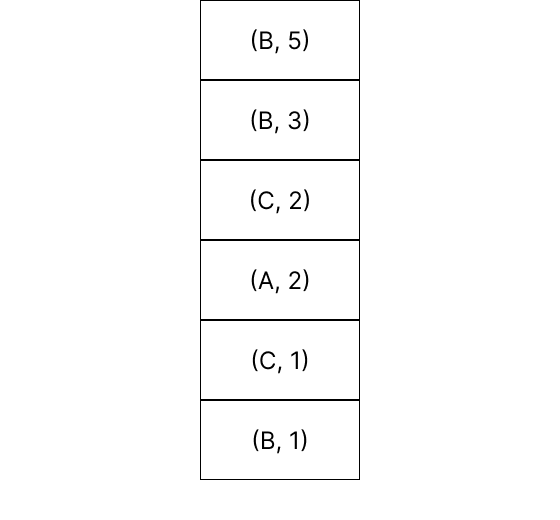
\includegraphics[width=0.6\textwidth]{images/MessageLog1.png}
    \caption{A message log with entries accumulating bottom-to-top in linear order}
    \label{fig:message-log-a}
  \end{subfigure}
  \begin{subfigure}{1\textwidth}
    \centering
    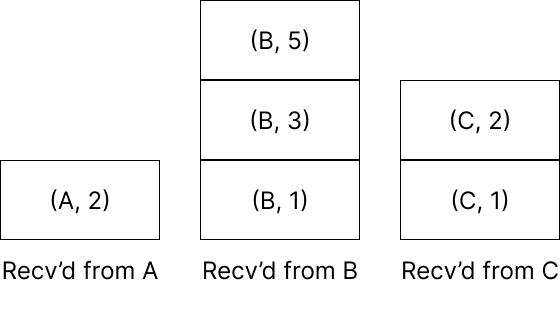
\includegraphics[width=0.6\textwidth]{images/MessageLog2.png}
    \caption{The same log shown with messages disaggregated by sender}
    \label{fig:message-log-b}
  \end{subfigure}
  \caption{A message log displayed linearly and disaggregated}
  \label{fig:message-log}
\end{figure}


\subsubsection{The Summary Vector and Its Invariant}
\label{sssec:tsae-summary-vectors}
Besides $\WL{P}$, the message propagation component maintains a
\emph{version vector} $\summaryVec{P}$ whose role is to quickly
communicate to other processes which messages $P$ has already
received. This structure is very similar to a vector clock (see
Section \ref{sssec:vector-clocks}) with a few differences. First, the
version of TSAE presented here happens to store physical, rather than
logical, clock values. A more essential distinction is that while a
vector clock tracks causality between events and increments the local
clock with each event, a version vector tracks the history of updates
to replicated data. The value $\summary{P}{P}$ tracks the set of
messages sent by $P$ and is incremented when $P$ sends a new message,
but not when $P$ receives a message from another process. As with
vector clocks, $\summary{P}{Q}$ can be thought of as $P$'s lower bound
view of $\summary{Q}{Q}$.

When $P$ submits a message to its own log, $\summary{P}{P}$ is
advanced to $\clock{P, t}$ and the message is timestamped with this
value. At some point in the future, $P$ contacts some other process
$Q$ to initiate an anti-entropy session. We conceptualize this process
as happening in three phases (setup, message exchange, and conclusion):
\begin{enumerate}
\item $\summary{P}{P}$ is advanced to $\clock{P, t}$. Symmetrically,
  $\summary{Q}{Q}$ is advanced to $\clock{Q, t}$. The parters exchange summary vectors.
\item For each process $X \in \AllProc$, $P$ sends to $Q$ the set of
  messages in $\WLat{P}{X}$ with timestamps greater than
  $\summary{Q}{X}$, if any. Likewise for each $X$ it receives all messages
  from $\WLat{Q}{X}$ with timestamps greater than $\summary{P}{X}$ and
  adds these to $\WLat{P}{X}$. The partners exchange signals to indicate
  when they are finished sending and receiving updates.
\item Much like a vector clock, $\summaryVec{P}$ is updated to the
  pointwise maximum of its current value and the value of
  $\summaryVec{Q}$ received from $Q$. Likewise $Q$ updates
  $\summaryVec{Q}$.
\end{enumerate}
The message log satisfies an invariant, termed the coverage property,
formalizing the role of $\summaryVec{P}$ as a summary of the contents
of $P$'s message log.
\begin{quote}
  \textbf{Coverage Property}: For all $Q$, $P$ has received
  all messages originating at $Q$ whose timestamps are less than the
  $Q^\textrm{th}$ entry in $P$'s summary timestamp vector.
  \[ \{m \in \WLat{Q}{Q} | \timestamp{m} \leq \summary{P}{Q} \} \subseteq \WLat{P}{Q} \]
\end{quote}
The previous subset relation is ``morally'' an equality---messages in
$\WLat{P}{Q}$ but not the subset are said to be ``early''---but only the
the subset property is required for correctness.\footnote{Section
  5.4.3 of Golding's thesis describes how a version of TSAE
  combined with an unreliable network-level multicast for optimization purposes can add
  messages to $\WLat{P}{Q}$ early.} Thus, besides forming a lower
bound of $\summary{Q}{Q}$, $\summary{P}{Q}$ can be thought of as an
\emph{upper} bound of the originating time, measured by $Q$'s clock,
of the last message $P$ received from $Q$. The coverage property
implies that $\summaryVec{P}$ provides complete information about the
(non-early) contents of $\WL{P}$.

The reader should convince themselves that the following inequalities
hold at all times for all $P$ and $Q$ (including when $P = Q$):
\[
  \max_{m \in \WLat{P}{Q}}\left({\timestamp{m}}\right) \leq \summary{P}{Q} \leq \summary{Q}{Q} \leq \clock{Q,t}.
\]

\begin{example}
  \label{ex:tsae}
  Figures \ref{fig:tsae1}---\ref{fig:tsae6} depict the evolution of
  TSAE executing across three distributed processes $A$, $B$, and
  $C$. The figures depict the following chain of events beginning at
  $t = 3$. Note that by $t = 9$, $A$ learns of writes submitted with
  $C$ without performing direct communication with $C$. The figures
  also depict acknowledgment vectors, shown in red, and what we later
  term the commit line, shown underlined. These are explained below.

  \begin{centering}
    \begin{tabular}{rl}\\
      \textbf{Time}    & \textbf{Action} \\
      $t = 1$   & $A$ submits a write                                            \\
      $t = 2$   & $B$ and $C$ submit writes                                      \\
      $t = 3$   & $B$ submits a write                                            \\
      $t = 4$ & $A$ and $B$ begin anti-entropy and swap summary vectors \\
      $t = 5$ & $B$ submits a new write  \\
      $t = 6$ & $A$ and $B$ finish anti-entropy, $C$ submits a write \\
      $t = 7$ & $B$ and $C$ begin anti-entropy, $A$ submits a write \\
      $t = 8$ & $B$ and $C$ finish anti-entropy, $A$ and $B$ begin anti-entropy \\
      $t = 9$ & $A$ and $B$ finish anti-entropy
    \end{tabular}
  \end{centering}
\end{example}

\begin{landscape}
  \begin{figure}%For some reason this empty figure adds vertical whitespace that makes the next figure positioned similarly to the ones that follow it.
  \end{figure}
  \begin{figure}[h]
    \centering
    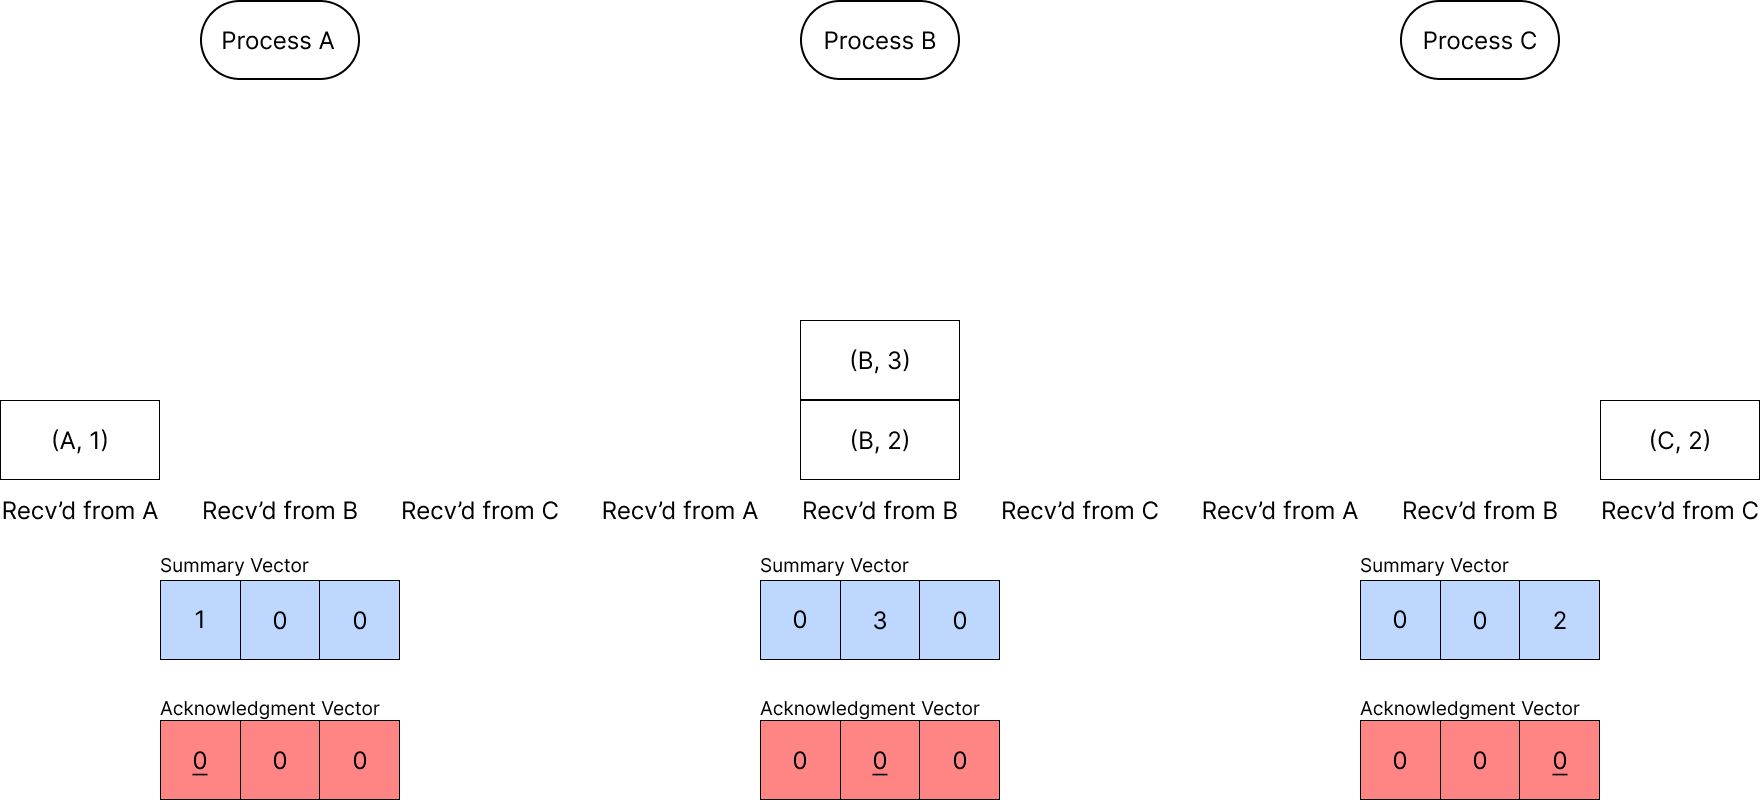
\includegraphics[width=1.4\textwidth]{images/tsaenew/TSAE3.png}
    \caption{TSAE at time $t=3$.}
    \label{fig:tsae1}
  \end{figure}
  \begin{figure}[h]
    \centering
    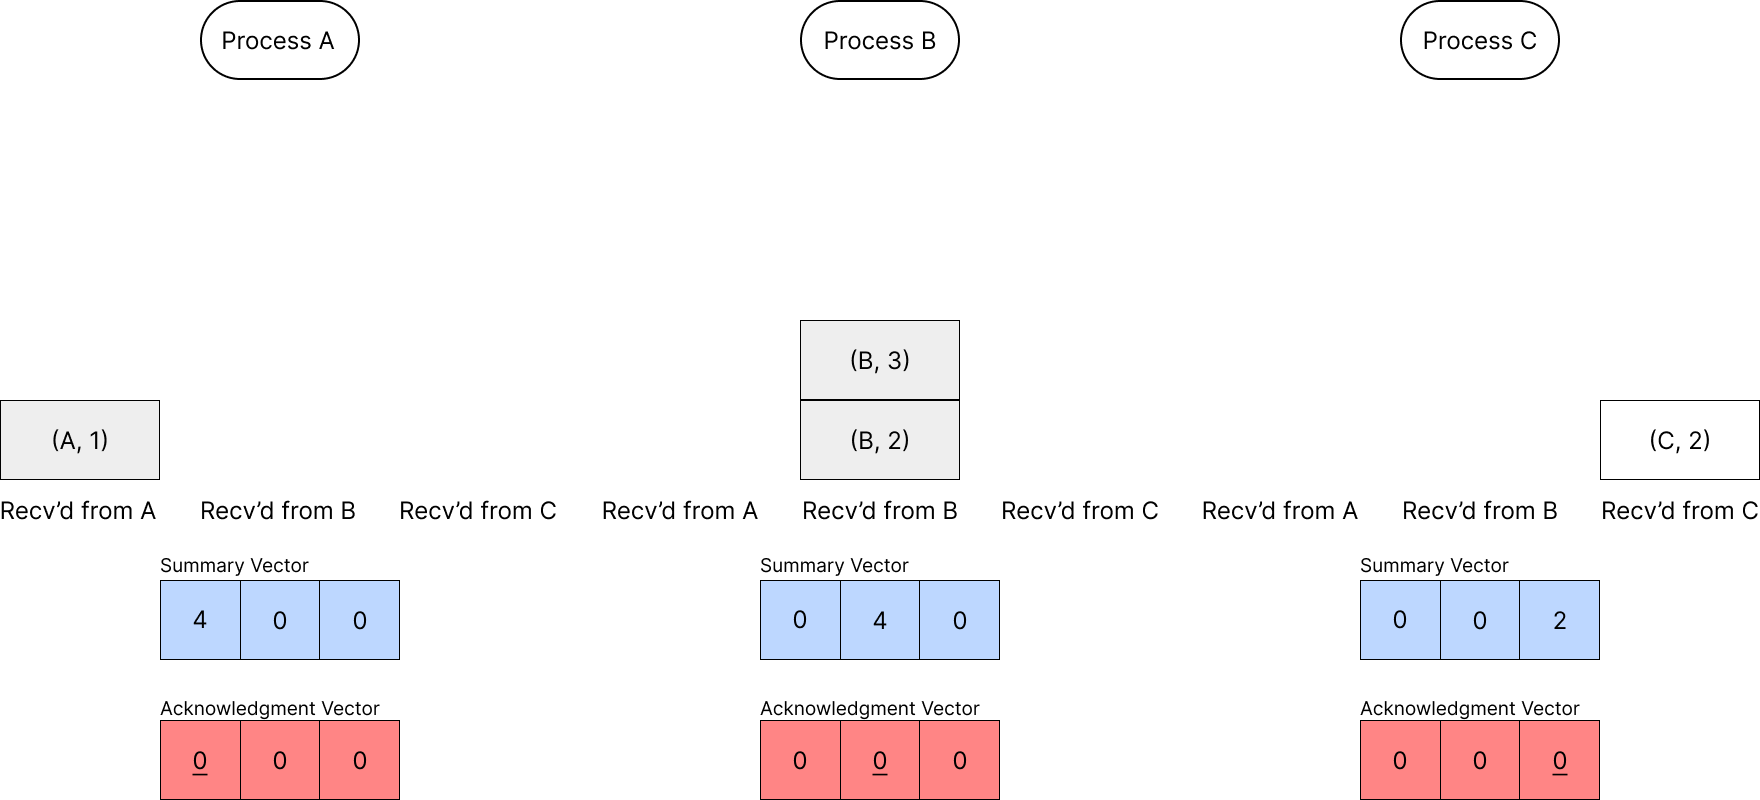
\includegraphics[width=1.4\textwidth]{images/tsaenew/TSAE4.png}
    \caption{TSAE at time $t=4$. $A$ advances $\summary{A}{A}$ to $\clock{A, t} = 4$ and likewise for $B$. After exchanging summary vectors, the participants decide to exchange the shaded messages.}
    \label{fig:tsae2}
  \end{figure}
  \begin{figure}[h]
    \centering
    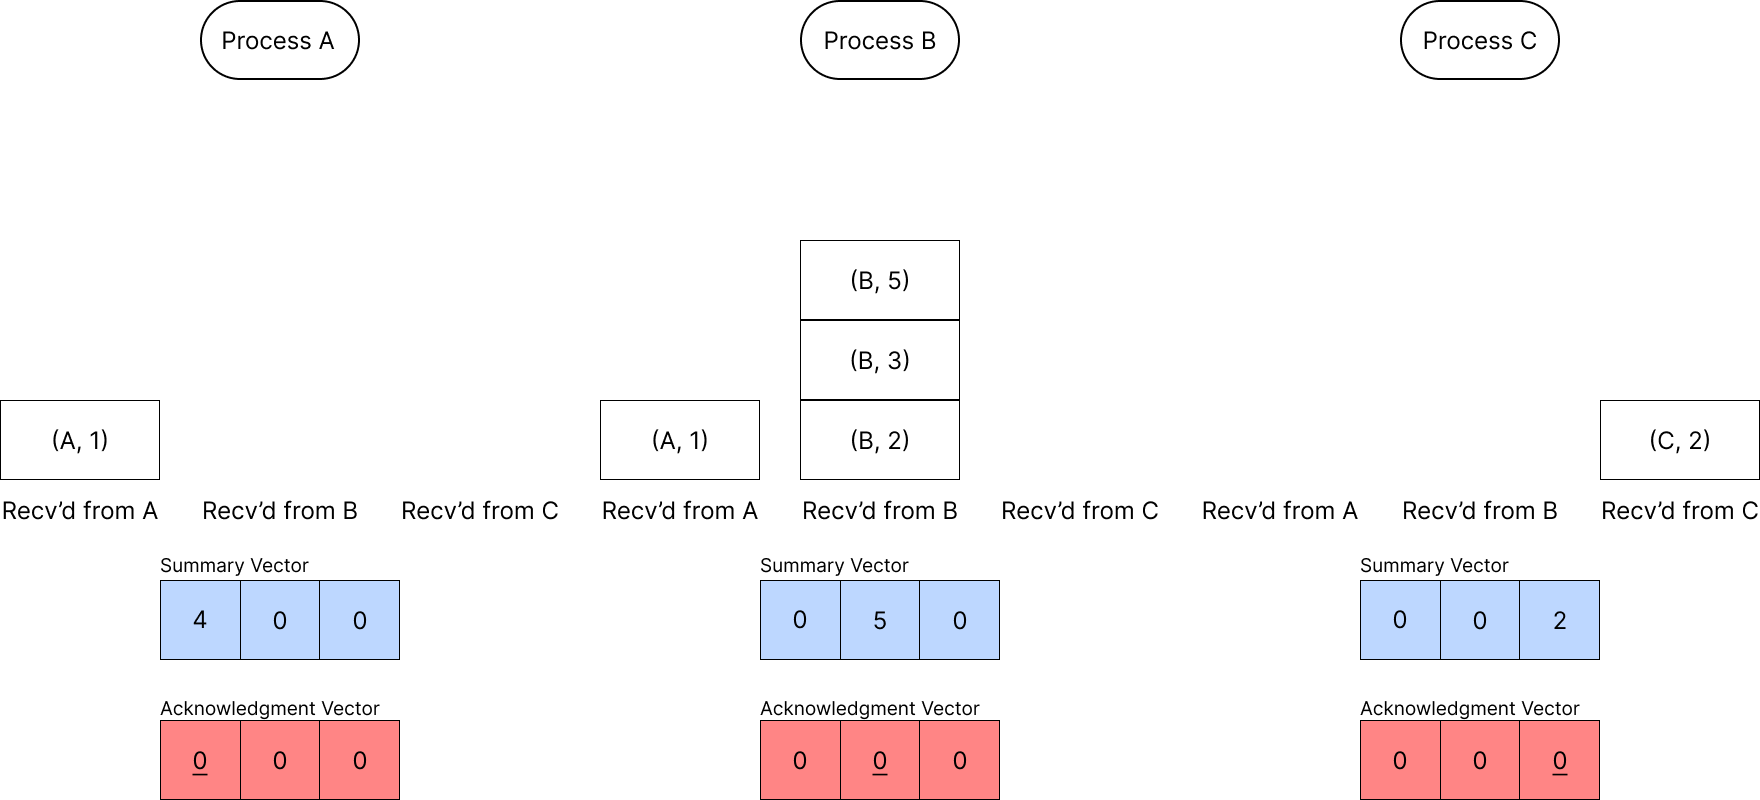
\includegraphics[width=1.4\textwidth]{images/tsaenew/TSAE5.png}
    \caption{TSAE at time $t=5$. $B$ has submitted a message with timestamp
      $t = 5$ while $A$ and $B$ are still engaged in an anti-entropy
      session in the background.}
    \label{fig:tsae3}
  \end{figure}
  \begin{figure}[h]
    \centering
    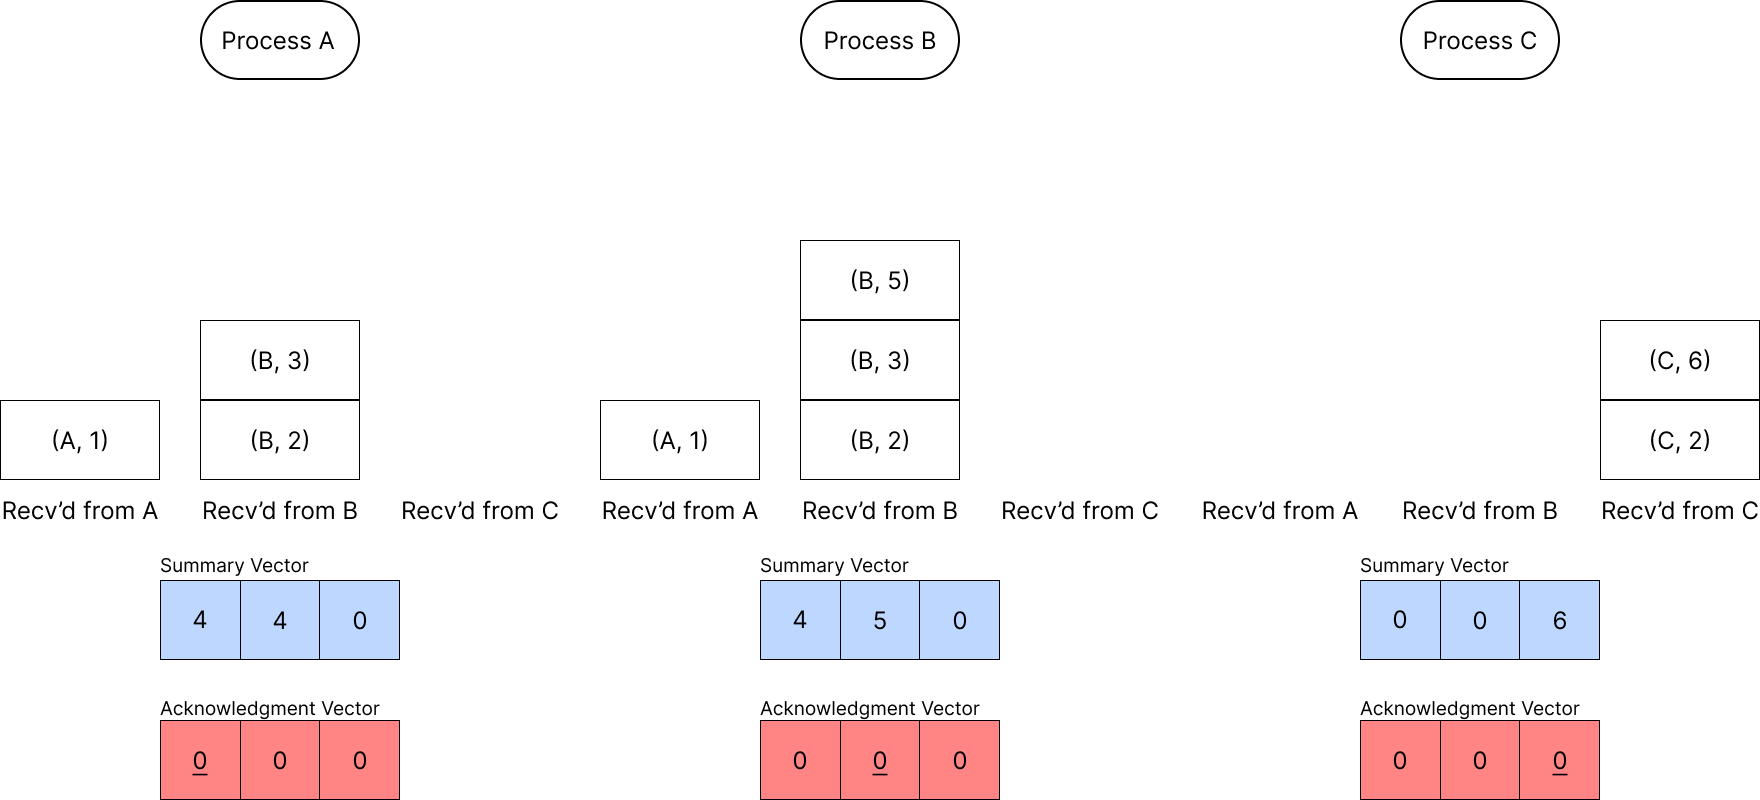
\includegraphics[width=1.4\textwidth]{images/tsaenew/TSAE6.png}
    \caption{TSAE at time $t=6$. $A$ and $B$ have finished their session and updated their summary vectors. Neither $A$ nor $B$ can update their commit line past $0$ because they both contain $\summary{}{C} = 0$, indicating they have not seen any messages from $C$. $C$ submits a message with timestamp $t = 6$.}
    \label{fig:tsae4}
  \end{figure}
  \begin{figure}[h]
    \centering
    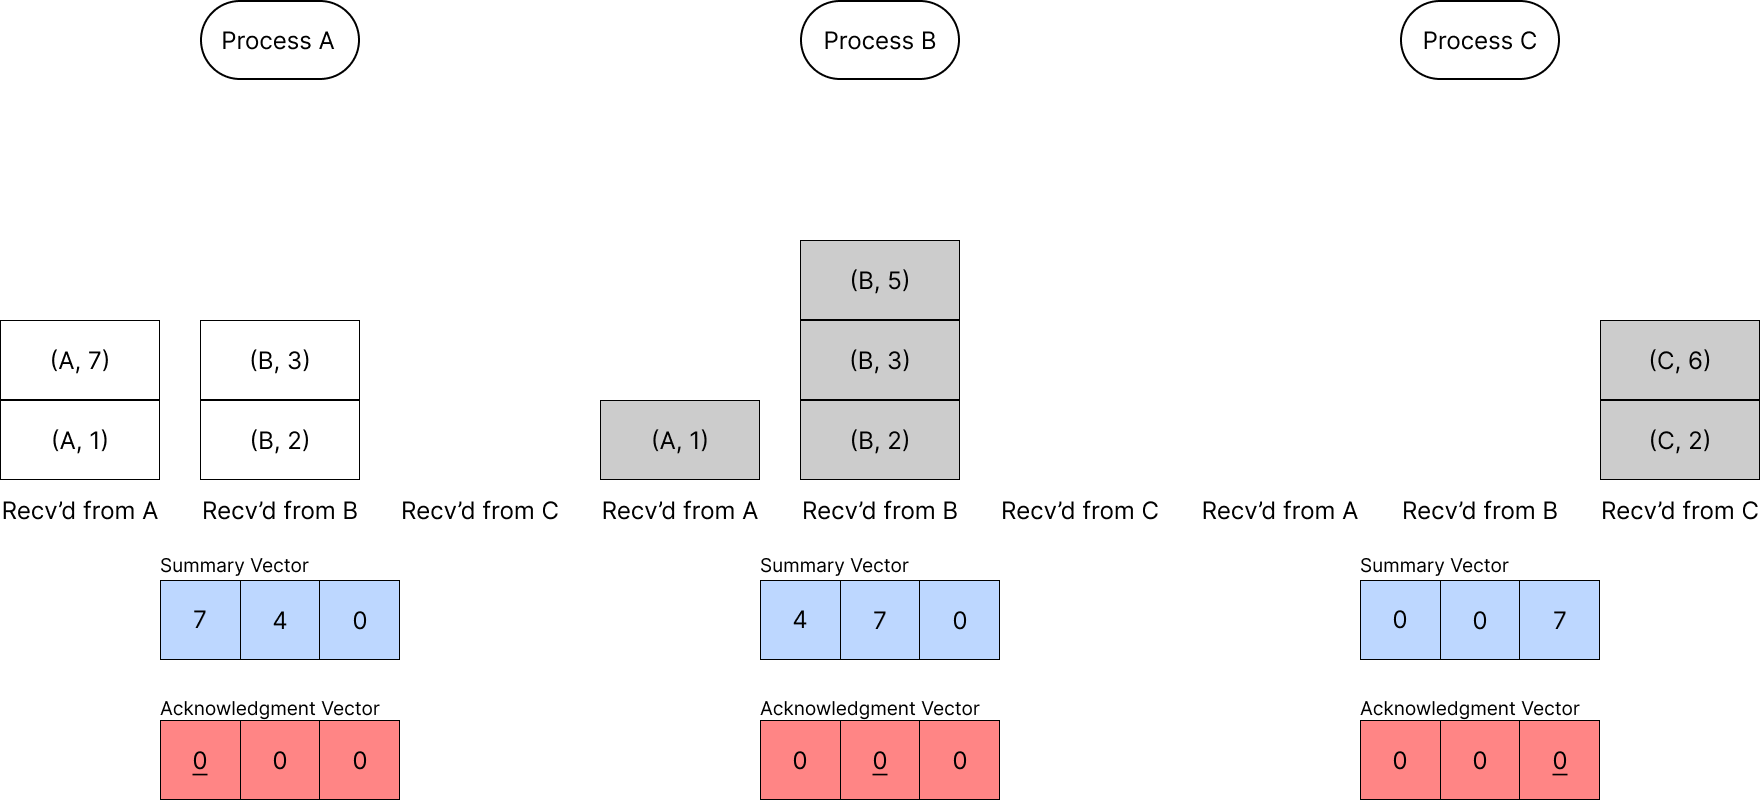
\includegraphics[width=1.4\textwidth]{images/tsaenew/TSAE7.png}
    \caption{TSAE at time $t=7$. $B$ and $C$ update and exchange summary vectors before deciding to exchange the shaded messages. $A$ submits a message with timestamp $t = 7$.}
    \label{fig:tsae4}
  \end{figure}
  \begin{figure}[h]
    \centering
    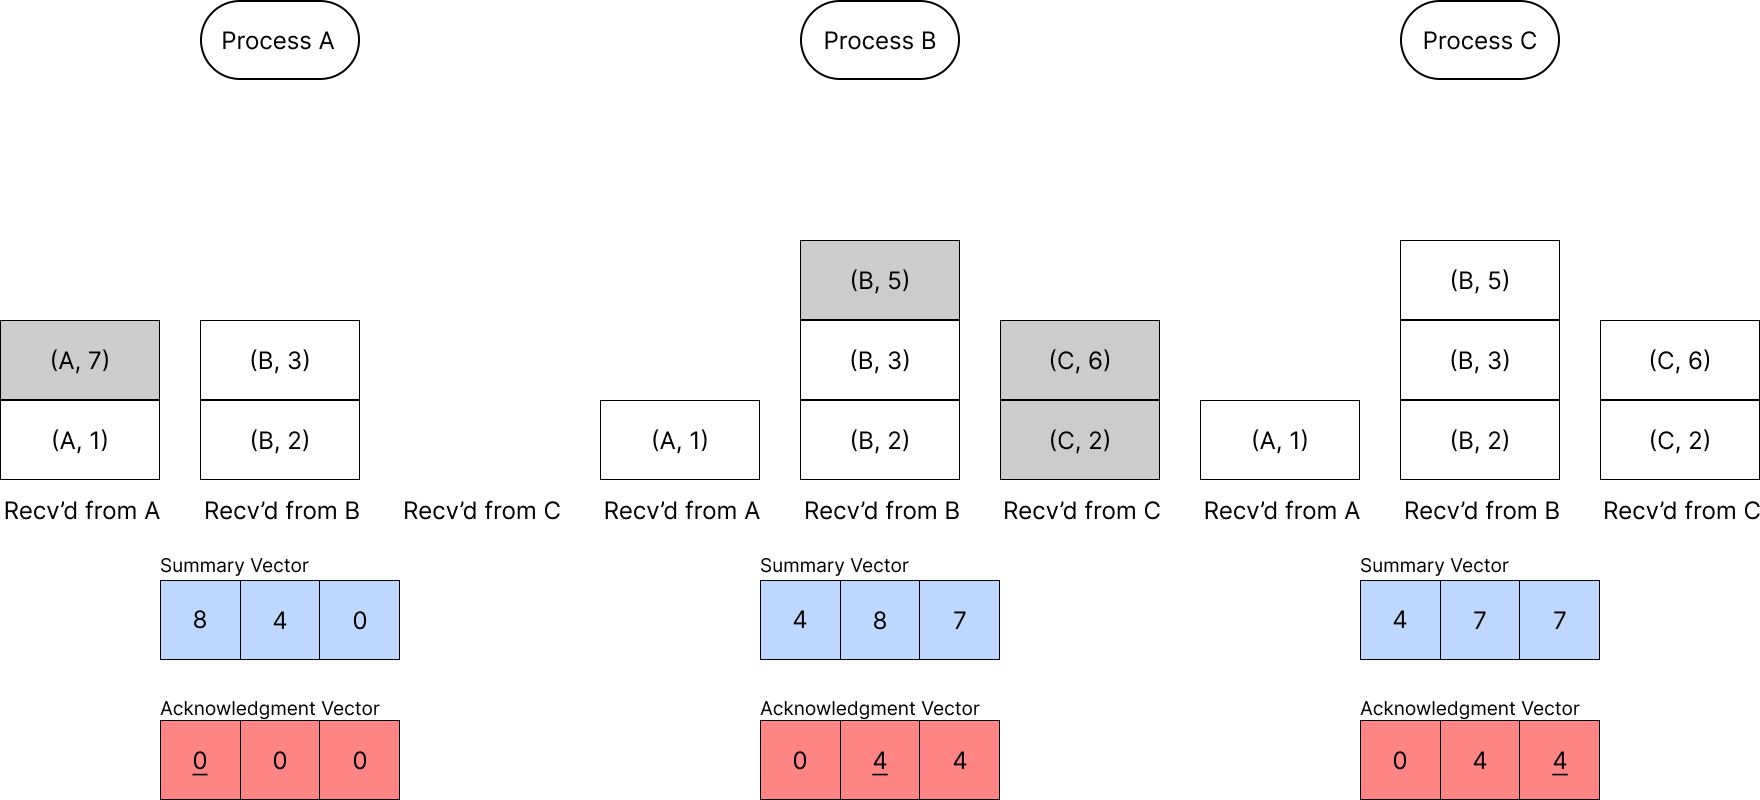
\includegraphics[width=1.4\textwidth]{images/tsaenew/TSAE8.png}
    \caption{TSAE at time $t=8$. $B$ and $C$ finish their anti-entropy session. Both sides can update their commit line to $4$, since they have seen all messages $m$ such that $\timestamp{m} \leq 4$. $A$ and $B$ begin anti-entropy, exchanging updated summary vectors and exchanging the shaded boxes.}
    \label{fig:tsae6}
  \end{figure}
  \begin{figure}[h]
    \centering
    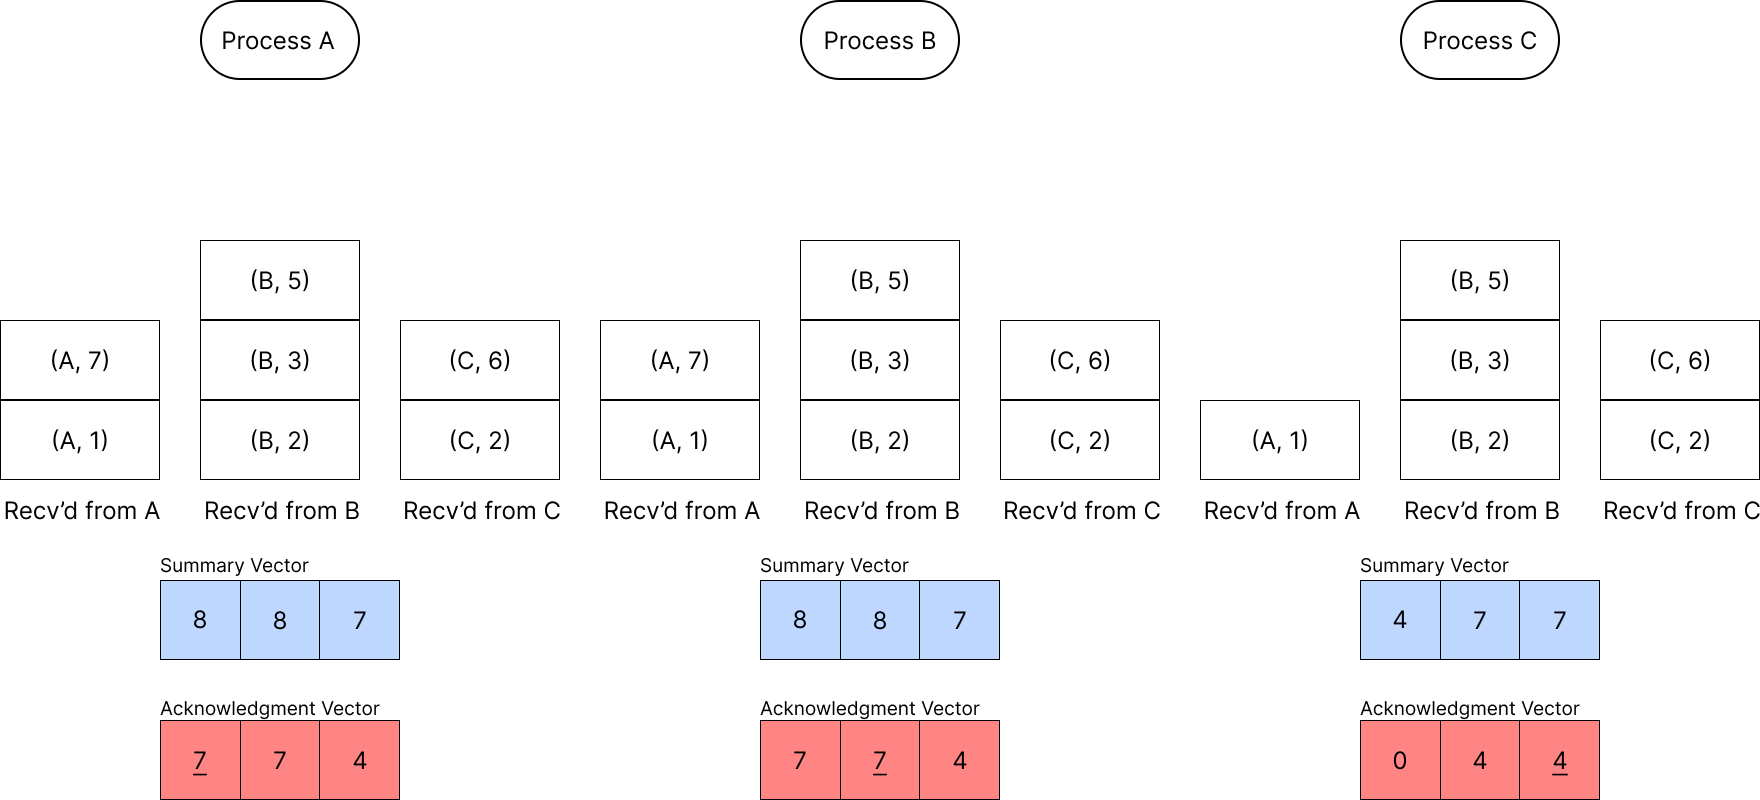
\includegraphics[width=1.4\textwidth]{images/tsaenew/TSAE9.png}
    \caption{TSAE at time $t=9$. $A$ and $B$ finish their anti-entropy
      session and have both seen all messages with timestampsless than
      or equal to $t = 7$. $B$ and $C$ can remove all messages with
      timestamps less than or equal to $4$ from their logs, since they
      both have minimum entries $\ack{}{C} = 4$. $C$ has received the
      same messages as $A$ and $B$, but has not witnessed $A$
      acknowledging them.}
    \label{fig:tsae6}
  \end{figure}
\end{landscape}

\subsubsection{The Acknowledgement Vector}
\label{sssec:tsae-acknowledgement}
$P$'s summary vector enables another process to quickly learn which
messages $P$ has seen. Additionally, $P$ must keep tabs on which
messages \emph{other} processes have seen. This information is
critical for the message ordering and log recycling components of
TSAE. Golding presents two ways to maintain this information, which
make different efficiency tradeoffs.

Arguably the simplest approach is for $P$ to maintain a local (lower
bound) copy, called $P$'s \emph{view}, of the summary vector of every
other process. During anti-entropy sessions, $P$ exchanges views with
its partner alongside its $\summaryVec{P}$, taking their pointwise
maximums afterwards. This leads to the idea of a version matrix, but
it has the downside of a per-process space requirement this is
quadratic in the size of the process group. This approach is
considered further in \ref{sssec:tsae-unsynchronized}.

The other mechanism presented by Golding requires each process $P$
to maintain an \emph{acknowledgement vector} $\ackVec{P}$. The basic idea
is to coarsely summarize $P$'s knowledge of other processes not with
its summary vector, but the minimal element in this vector, a scalar,
which is stored in $\ack{P}{P}$. For reasons explained in
Section \ref{ssec:consistency-units}, this value is called $P$'s \emph{commit
  line}. Periodically, $P$'s commit line is updated to the minimal
timestamp in its summary vector,
$\min_{X \in \AllProc} \left(\summary{P}{X}\right)$.  For correctness,
the invariant required of $\ack{P}{P}$ is that it is always a lower
bound of this minimum.
\begin{quote}
  \textbf{Acknowledgement Property}: $P$'s commit line is less than or
  equal to the minimum value in $P$'s summary vector.\footnote{The
    inequality here can be thought of as morally an equality. It may
    be a strict inequality while $P$ is updating $\summaryVec{P}$
    before recomputing its minimum. Recall $P$ may be multi-threaded
    with multiple anti-entropy sessions affecting $\summaryVec{P}$ at
    the same time.}
  \begin{equation*}
    \ack{P}{P} \leq \min_{X \in \AllProc} \left(\summary{P}{X}\right)
\end{equation*}
\end{quote}

Acknowledgment vectors are updated during anti-entropy sessions much
like vector clocks and version vectors.
\begin{enumerate}
\item At the beginning of the session, $\ack{P}{P}$ is updated to
  $\min_{X \in \AllProc} \left(\summary{P}{X}\right)$. Symmetrically
  for $Q$. $P$ and $Q$ exchange acknowledgement vectors alongside
  their summary vectors.
\item At the end of the session, $P$ sets $\ackVec{P}$ and to the
  pointwise maximum of its current value and the value of $\ackVec{Q}$
  received from $Q$. $Q$ updates $\ackVec{Q}$ symmetrically.
\end{enumerate}
Note that $\ack{P}{Q} \leq \ack{Q}{Q}$ at all times for all $P$ and
$Q$.

Slightly different from Golding's presentation of the protocol, the
figures discussed in Example \ref{ex:tsae} also demonstrate an
optimization that takes advantage of the fact that summary vectors are
updated at the end of anti-entropy sessions. After updating these
vectors to their pointwise maximum, we immediately recompute
$\ack{P}{P}$, setting it to
$\min_{X \in \AllProc} \left(\summary{P}{X}\right)$. Furthermore,
$\ack{P}{Q}$ is set to this value. Symmetrically, $Q$ updates
$\ack{Q}{Q}$ and $\ack{Q}{P}$. Note that this preserves the preserves
the invariant that $\ack{P}{Q}$ and $\ack{Q}{P}$ are lower bounds of
$\ack{Q}{Q}$ and $\ack{P}{P}$, respectively, provided the
implementation ensures $P$ increments $\ack{P}{Q}$ only if $Q$
increments $\ack{Q}{Q}$ and vice versa. This optimization advances
acknowledgment vectors (and later, version matrices) more often than
Golding's presentation, which allows the ordering and purging
mechanisms (explained below) to progress more quickly.

The following two lemmas explain the utility of $\ackVec{P}$ as a way
of estimating global state.

%%%%%%%%%%%%%%%%%%%%%%%%%%%%%%%%%%%%%%%%%%%%%%%%%%%%%%%%%%%%%%%%
\begin{lemma}
  \label{lem:commitline}
  $P$ has received all messages (from any sender) with timestamps less
  than or equal to its commit line $\ack{P}{P}$.
\end{lemma}
\begin{proof}
  Let message $m$ originate at $Q$ with timestamp
  $\timestamp{m} \leq \ack{P}{P}$. Then
  \[\timestamp{m} \leq \ack{P}{P} \leq \min_{X \in
      \AllProc}\left(\summary{P}{X}\right) \leq\summary{P}{Q}.\] The
  coverage property implies $m \in \WL{P}$.
\end{proof}
%%%%%%%%%%%%%%%%%%%%%%%%%%%%%%%%%%%%%%%%%%%%%%%%%%%%%%%%%%%%%%%%

%%%%%%%%%%%%%%%%%%%%%%%%%%%%%%%%%%%%%%%%%%%%%%%%%%%%%%%%%%%%%%%%
\begin{lemma}
  \label{lem:ack-vector}
  For all messages $m$, if $\timestamp{m} \leq \ack{P}{Q}$, then $Q$
  has received $m$.
\end{lemma}
\begin{proof}
  Now $\timestamp{m} \leq \ack{P}{Q} \leq \ack{Q}{Q}$. By Lemma
  \ref{lem:commitline}, $Q$ has received $m$.
\end{proof}
%%%%%%%%%%%%%%%%%%%%%%%%%%%%%%%%%%%%%%%%%%%%%%%%%%%%%%%%%%%%%%%%


When a message $m$ in the write log satisfies
$\timestamp{m} \leq \ack{P}{P}$, $P$ is said to have
\emph{acknowledged} $m$. In light of Lemma \ref{lem:commitline}, all
acknowledged messages have been received. The converse does not hold,
since a received message will not be acknowledged until each entry in
$\summaryVec{P}$, not just the entry of its sender, is greater than
$\timestamp{m}$. We now explain how acknowledged messages can be
delivered to the application and ultimately purged from $\WL{P}$,
before considering the matrix-based alternative to acknowledgement
vectors.

\subsubsection{Message Ordering}
\label{sssec:tsae-message-ordering}
TSAE guarantees that messages will eventually be received by all other
processes, but ordering of these messages in different processes' logs
may vary. In some applications this is acceptable, but other
applications require more control over delivery order. Recall from
Section \ref{ssec:message-ordering} that to enforce ordering
guarantees, a distinction is made between message receipt and
delivery. A message ordering layer buffers incoming messages upon
receipt, giving time for slower messages to catch up to faster ones,
before delivering them to the application in a predictable order.

The message ordering component of TSAE periodically inspects $\WL{P}$
and delivers messages to $P$ when ready. To enforce total order, this
component delivers all messages whose timestamp is less than or equal
to $P$'s commit line. That is, the set of messages satisfying
\begin{equation}
  \label{eq:tsae-message-ordering-condition}
  \timestamp{m} \leq \ack{P}{P}
\end{equation}
These messages are delivered to $P$ in order of their timestamps, using
the identifiers of their senders to resolve ties. The correctness of
this approach follows from Lemma \ref{lem:commitline}, since $P$ has
seen all messages whose timestamp is less than $\ack{P}{P}$, and
therefore the stream of delivered messages will not have any ``gaps.''
This mechanism for enforcing a total order dates back to the
introduction of scalar clocks \cite{1978:lamportclocks}. Golding also
describes straightfoward mechanisms to enforce causal and total-causal
order in Section 5.5 in his dissertation.

The ordering component guarantees messages will eventually be
delivered.
\begin{lemma}
  Every message will eventually be delivered to $P$ by TSAE.
\end{lemma}
\begin{proof}
  Assuming periodic anti-entropy sessions, the process in
  \ref{sssec:tsae-message-log} ensures each message is eventually
  received by $P$ and each value of the form $\summary{P}{Q}$
  eventually increases. Thus, the minimum entry in $\summaryVec{P}$
  will eventually increase beyond $\timestamp{m}$, so each $m$ will be
  delivered as long as the ordering component runs periodically.
\end{proof}

Golding's assumption of loose clock synchronization is driven by a
practical need to ensure messages are delivered in a timely fashion
instead of just eventually. For example, if $Q$ has an exceptionally
slow clock compared to other processes, then $\summary{P}{Q}$ will
remain the minimum element in $\summaryVec{P}$ for a long time. During
this time, only messages from $Q$ will be delivered to $P$, as all
other messages would have timestamps greater than $Q$'s clock.

A message simply cannot be removed from the write log after being
delivered to $P$, because some of the messages in $\WL{P}$ may still
need to be propagated to new recipients during anti-entropy in the
future. Consequently, the ordering component must perform bookkeeping
to remember which messages in the log have already been delivered.

\subsubsection{Message Purging}
\label{sssec:tsae-message-purging}
As presented, the message log at each host grows without limit, so it
requires an unbounded amount of storage. Thus, a separate log
recycling process can be used to remove old entries when they are no
longer required.

There are two requirements for a message to be safe to delete. First,
it clearly must have been delivered to $P$ already. Additionally, it
must have been received by all other processes---otherwise it might be
one of the messages $P$ should send in a future anti-entropy
session. $P$ will know a message $m$ has been acknowledged by all
other processes when its timestamp is less than or equal to $P$'s
\emph{purge line}, defined as the minimum entry in the acknowledgment
vector:
\begin{equation}
  \label{eq:tsae-message-purging-condition}
  \timestamp{m} \leq \min_{X \in \AllProc} \left( \ack{P}{X} \right)
\end{equation}

The safety of this deletion procedure is proven by the following
lemma.
%%%%%%%%%%%%%%%%%%%%%%%%%%%%%%%%%%%%%%%%%%%%%%%%%%%%%%%%%%%%%%%%
\begin{lemma}[Log purging]
  \label{lem:purge}
  $P$ can safely discard all messages in $\WL{P}$ with timestamps less
  than or equal to its purge line, after they have been delivered.
\end{lemma}
\begin{proof}
  Let message $m \in \WL{P}$ originate at $R$ with timestamp less than
  $P$'s purge line. Now the following inequalities hold for all $Q$:
  \[ \timestamp{m} \leq \min_{X \in \AllProc}\left(\ack{P}{X}\right)
    \leq \ack{P}{Q}.\] Therefore, by Lemma \ref{lem:ack-vector}, $m$
  has been delivered to $Q$. Since $Q$ is arbitrary, $m$ has been
  received everywhere (where it will eventually be delivered as well)
  and can be purged from $\WL{P}$ to reclaim storage space.
\end{proof}
%%%%%%%%%%%%%%%%%%%%%%%%%%%%%%%%%%%%%%%%%%%%%%%%%%%%%%%%%%%%%%%%
\begin{comment}
For contrast, suppose $m$ has a timestamp greater than $\ack{P}{Q}$.
Then without knowing the current value of $\summary{Q}{R}$ there is no
guarantee $\timestamp{m}$ is less than this value. In this case,
deleting $m$ from $\WL{P}$ might prevent $Q$ from ever receiving $m$.
\end{comment}

Because every message is eventually delivered and acknowledged by each
process, $P$ will eventually be able to remove each message from its
log. It is still possible for $\WL{P}$ to grow without bound if the
rate of message arrival exceeds the speed at which they are
purged. This might occur during periods of heavy usage or during a
network partition, as $P$ will eventually become unable to advance
$\ack{P}{Q}$ further if $Q$ is on the other side of a partition. The
storage requirements of the message log in a particular use case and
environment should be measured empirically as part of an application
optimization strategy.

\subsubsection{TSAE using Version Matrices}
\label{sssec:tsae-unsynchronized}
If clocks are not approximately synchronized, the clock value at one
process may greatly exceed that of another. Because the minimal entry
in $\summaryVec{P}$ is used to concisely summarize which messages $P$
has seen, if $Q$ has a very fast clock, messages $P$ receives from $Q$
may not ever be acknowledged, since the minimal entry will remain less
than $\summary{P}{Q}$ for a long time.

Rather than concisely summarizing which messages $P$ has seen using
the minimum entry in $\summaryVec{P}$, the entire vector offers a more
precise measure. For $P$ itself, that means tracking what other
process know about by keeping a copy of $\summaryVec{Q}$ for each $Q$
in the system. Thus, we do away with $\ackVec{P}$ and track what other
processes know using a vector-of-vectors, to say a matrix, that we
call $\ackMatrix{}$. Since $\summaryVec{}$ is a version vector, then
$\ackMatrix{}$ can be called a version matrix.

With this implementation strategy, $\ackMatrix{P}[P]$ stores $P$'s
summary vector. $\ackMatrix{P}\left[Q\right]$ represents $P$'s lower
bound estimate of $Q$'s summary vector, with $\ackMatrix{P}[Q][R]$
providing a lower bound estimate of the greatest timestamp of any
message $Q$ has received from $R$. Matrices are exchange during
anti-entropy sessions just as before, with both sides taking the
pointwise maximum after.

Altogether, $P$ applies the following (conservative) policies:
\begin{itemize}

\item A message with timestamp $m$ is ready to be delivered to $P$ by a total
  ordering component when the following analogue of \eqref{eq:tsae-message-ordering-condition} holds:
  \[\timestamp{m} \leq \min_{X \in \AllProc} \left(\ackMatrix{P}[P][X]\right)\]
\item A message $m$ originating at $R$ has been
  received by $Q$ when the following condition holds:
  \[ \timestamp{m} \leq \ackMatrix{P}[Q][R] \]
\item A message $m$ originating at $R$, after being delivered to $P$,
  can be purged from the log when the following analogue of
  \eqref{eq:tsae-message-purging-condition} holds:
  \[ \timestamp{m} \leq \min_{X \in \AllProc}\ackMatrix{P}[X][R]\]
\end{itemize}

Of course, matrices require $\Theta(n^2)$ storage at each site for a
process group with $n$ members, which quickly becomes untenable for
systems where $n$ is on the order of 1,000 or greater.

\subsection{Consistency Unit Framework}
\label{ssec:consistency-units}

Using periodic timestamped anti-entropy sessions to synchronize
replicas only provides a progress guarantee: all messages will
eventually be received, acknowledged, delivered, and purged from the
log of all processes, assuming the devices do not fail and network
partitions do not last forever. This implements a \emph{weak
  consistency} model: using TSAE to replicate state allows replicas to
diverge, but ensures they will eventually converge to an agreement if
allowed to communicate, at least if new updates do not outpace the
rate of convergence. Unfortunately, this property does not say
anything about how far apart replicas might diverge in the meantime.

This section summarizes the key ideas behind \emph{continuous}
consistency, with a particular focus on the conit (``consistency
unit'') model proposed by Yu and Vahdat
\cite{2000tact,2000tactalgorithms,10.5555/1251229.1251250,DBLP:conf/icdcs/YuV01,2002tact}. Continuous
consistency is motivated by the observation that real-world
applications can generally tolerate some level of divergence of
replicated data, especially in exchange for greater performance and
availability. Intuitively, applications can operate with replicas that
deviate from their ``ideal'' value by at most some margin of error
$\epsilon \geq 0$. However, applications have unique data models and
measure this error in different ways, so building a general framework
to enforce quantitative error bounds on replicas without making
specific assumptions about the nature of the data is challenging.

The conit framework strikes a desirable balance between being general
enough to work in applications with very different data models, and
practical enough to efficiently enforce error bounds with
straightforward protocols. We describe it now in terms of its system
model (\ref{sssec:conit-system-model}), its three dimensions of
consistency
(\ref{sssec:conit-numerical-consistency}---\ref{sssec:conit-real-time-consistency}),
and possible extensions (\ref{sssec:conit-extensions}).


\subsubsection{System Model}
\label{sssec:conit-system-model}
The system consists of processes in $\AllProc$ that replicate a shared
database (more generally, any kind of replicated state
machine). Processes perform two types actions, read or write requests,
as in Section \ref{ssec:shared-memory}. We call actions of both types
\emph{accesses}. The initial database state at each replica is
$\Dinit$. Accesses potentially contain multiple instructions, such as
in a relational database transaction. Recall that a history is an
ordered sequence of read and write accesses. The \emph{local history}
of a process $P$, denoted $H_P$, is the sequence of accesses $P$ has
applied to $\Dinit$ since the start of the application. A read access
submitted to $P$ by a user is always handled locally by $P$ without
involving other processes. A write access submitted to $P$ is applied
locally and additionally propagated to all other replicas using TSAE
as the messaging framework.

Write accesses encode an action to be performed against a database
image (rather than the final value the data after performing that
action). The result of applying write action $w$ to a database state
$D$ is denoted $D + w$. Let $D + H$ denote the result of applying each
of the writes in $H$ to $D$ in history order. Each process $P$
maintains a write log, $\WL{P}$, containing the history of all writes
applied to its local database image in the order they were applied
(making $\WL{P}$ equivalent to the local history of $P$, $H_P$,
restricted to write requests). Note that the current state of $P$ is
uniquely determined by a combination of the starting state ($\Dinit$)
and $\WL{P}$:
\[  D_P = \Dinit + \WL{P} \label{eq:conit-DP} \]


The initial database state at each replica is $\Dinit$.  Write
accesses encode an action to be performed against a database image
(rather than the final value the data after performing that
action). The result of applying write action $w$ to a database state
$D$ is denoted $D + w$. Let $D + H$ denote the result of applying each
of the writes in $H$ to $D$ in order.  Each process $P$ maintains a
write log, $\WL{P}$, containing the history of all writes applied to
its local database image in the order they were applied (making
$\WL{P}$ equivalent to the local history of $P$ restricted to write
requests). Note that the current state of $P$ is uniquely determined
by a combination of the starting state ($\Dinit$) and $\WL{P}$. In the
above notation, the current value $D_P$ of $P$'s replia is
$\Dinit + \WL{P}$. When a read request is submitted to $P$, the
requested value is read immediately from $D_P$ and returned to the
caller. When a write request $w$ is submitted, the action is performed
against the local replica and $w$ is added to $\WL{P}$. With either
type of access, $P$ is said to be the \emph{originating replica}, and
all other processes are \emph{remote}. The value of $D_P$ is said to
be the \emph{observed state} of the access.  We assume some ECG
history as a reference point. The \emph{ideal result} of an access $a$
is the value $\Dinit + \PH_\textrm{a}$.  The following equations hold.

When a read request is submitted to $P$, the requested value is read
immediately from $D_P$ and returned to the caller. When a write
request $w$ is submitted, the action is performed against the local
replica and $w$ is added to $\WL{P}$. With either type of access, $P$
is said to be the \emph{originating replica}, and all other processes
are \emph{remote}. The value of $D_P$ is said to be the \emph{observed
  state} of the access.

Timestamped anti-entropy is used to propagate writes to remote
replicas, with $\WL{P}$ acting as the message log. When a remote
replica $Q$ receives new writes, they are added to $\WL{Q}$ and
applied to $Q$'s local image as well. Now, replicated state machines
will reach the same final state on two conditions. First, all replicas
learn about each write, and second, all replicas execute writes in the
same order. TSAE by itself ensures the first condition, since every
process will eventually learn about every write. However, we know that
TSAE alone does not provide ordering guarantees. Thus, the data model
should provide a mechanism for rolling back (undoing) writes that have
been applied to $D$. When a write is first accepted, it is said to be \emph{uncommitted}
and applied \emph{tentatively} to the local replica. Uncommitted
writes are subject to being rolled back and reapplied in a different
order later, possibly with different results. Eventually, the write
becomes \emph{committed}, after which it is never rolled
back. Committed writes are applied in the same order at all
replicas. Taking the place of the message ordering component, a write
committment component is responsible for ultimately committing writes
accesses. Commitment is an adaptation of the total ordering mechanism
in \ref{sssec:tsae-message-ordering}.

\subsubsection{Ideal Histories}
To define quantify deviation from strong consistency, we must give a
few definitions. Recall the notion of external order (Definition
\ref{def:external-order}): an access $A$ externally precedes $A'$ if
$A$ has returned to the caller before $A'$ is invoked. Yu and Vahdat
also define a notion of causality:
\begin{definition}[Causal precedence of accesses]
  \label{def:conit-causal-precedence}
  $A$ \emph{causally precedes} $A'$ if $A$ was already in the local
  history of the originating replica when $A'$ was submitted, and so
  could have influenced how $A'$ executed.\footnote{At face value it
    may seem that if $A$ is in a replica's write log before $A'$, then
    it must have completed before $A'$ started and thus already
    precedes $A'$ externally. However, if these represent long-running
    database transactions, it is possible that $A$ logically takes
    effect before $A'$ at some replia, though the two transactions may
    be physically concurrently.}
\end{definition}

With these definitions, we can define a strongly consistent execution
as a reference point for measuring deviation.

\begin{definition}[Ideal image]
  An ECG (externally consistent, causally consistent, global) history
  is the set of accesses across the system arranged in some total
  order that respects both external and causal order as defined above.
\end{definition}
Definitions below are given with respect to some ECG
history. Intuitively, the condition expected from the conit framework
is that at any moment in time, there is some ECG history such that all
replicas diverge from the ECG history by at most some error bound.
 We assume some ECG history as a reference
point. The \emph{ideal result} of an access $a$ is the value
$\Dinit + \PH_\textrm{a}$.  The following equations hold.
\begin{gather}
  \Dideal = \Dinit + \WL{\textrm{ideal}} \label{eq:conit-Dideal}
\end{gather}

There are essentially three reasons

\subsubsection{Conits}
The intention of the conit framework is this: at any moment in time,
there exists some ECG history of system accesses such that no
individual replica deviates from too far this history. To define what
it means to deviate, we now define conceptual units of data whose
relative (in)consistency can be quantified.

A read request depends on a set of conits $\mathcal{F}$. That is to
say, it assumed that the read will return the same value for any two
database images $D$ and $D'$ such that $F(D) - F(D') = 0$ for each
conit $F$ in $\mathcal{F}$. This access will be associated with a
consistency requirement for each conit in $\mathcal{F}$.

We write $\WL{P}|_\mathcal{F}$ to indicate the history of $P$
restricted to just the messages with non-zero weight on any of the
conits in the set $\mathcal{F}$.

The application can specify the consistency requirements for each
conit along a three-dimensional axis:
\[\textrm{Consistency} = \langle \textrm{Numerical error,
    \textrm{Order error}, \textrm{Staleness}} \rangle.\]

Anti-entropy can be push- or pull-based. To push updates from $P$ to
$Q$, $P$ obtains $Q$'s summary vector $\summaryVec{Q}$ and pushes all
unseen messages in $\WL{P}$ to $Q$. To pull updates, $P$ sends its
version vector and requests any messages in $\WL{Q}$ that $P$ has not
seen.

Numerical error bounded by a \emph{push}-approach: $P$ may have to
block during a request in order to proactively inform $Q$ about the
update before it can be applied. This consists of $P$ obtaining $Q$'s
current summary vector and then forwarding messages in $P$'s write log
that $Q$ hasn't seen.

Take, say, an application for disseminating the most up-to-date
visualization of the location of a fire front. A client may find this
it acceptable for this information to appears 30 seconds out of date
to a client, but unacceptable if it is 30 minutes out of date. For
example, firefighters who are very close to a fire have a lower
tolerance for stale information than a central client keeping only a
birds-eye view of several fire fronts simultaneously. The \emph{real
  time staleness} metric allows each process $P$ to bound the maximum
amount of time between an access affecting a conit being issued and
$P$ seeing that access.

Real-time staleness and order error are both bounded by a
\emph{pull}-based approach: $P$ may have to block during an operation
while contacting other sites in order to request information from
them.

\subsubsection{Numerical consistency}
\label{sssec:conit-numerical-consistency}
We imagine that a conit $F$ is associated with a valuation function,
\[
  \Val^F\colon \mathsf{Database\ Image} \to \mathbb{R}
\]
that maps a database state to some real value. Then,
$\Val^F(D)$ is thought of as the value of conit $F$ for a
database state $D$. Let $V_P$ denote the current value of $F$ at $P$'s
replica $D_P$. Let $\Videal$ represents the value of $F$ at $\Dideal$.

Each write update $w$ is associated with a value, $\NumWeight^F(w)$,
for each conit $F$, codifying the effect of $F$ of applying $w$ to a
database. That is, $w$ represents the value
\[ \NumWeight\left(w, F\right) = \Val^F(D + w) - \Val^F(D), \] which
we assume is independent of $D$ itself. Note that $F$ distributes over
$+$ in the sense that $F(D + w) = F(D) + \NumWeight(w, F)$. Combining
this with Equations \eqref{eq:conit-DP} and \eqref{eq:conit-Dideal}
gives
\begin{gather}
  V_P = V_{\textrm{init}} + \sum \{\NumWeight(w, F) | w \in \WL{P}\} \\
  \Videal = V_{\textrm{init}} + \sum \{\NumWeight(w, F) | w \in \WL{\textrm{ideal}}\}
  %\sum \{\NumWeight(w) | w \in \WL{P}\} = \left(\mathsf{SeenPosWeight}_F^P\left(X\right) + \mathsf{SeenNegWeight}_F^P\left(X\right)\right) \\
\end{gather}

We assume each process $P$ maintains a conservative estimate, called
its \emph{view}, of which writes originating at $P$ have been received
by each other process. $P$'s view of $Q$ is denoted by
$\View{P}{Q}$. This estimate must be safe, meaning $P$ will not assume
$Q$ has received a message that it has not.
\begin{quote}
  \textbf{Approximate local knowledge of remote knowledge}: For each $Q$,
  $P$ can compute a set $\View{P}{Q}$ subject to the following
  invariant:
  \begin{equation*}
    \View{P}{Q} \subseteq \WL{Q}(P)
  \end{equation*}
  $P$ must also implement a mechanism to advance its view by
  synchronizing with $Q$.
\end{quote}
Its view also provides $P$ with an estimate of the messages it has
originated that $Q$ has not received yet, namely
$\WLat{P}{P} \setminus \View{P}{Q}$. Yu and Vahdat do not prescribe a
particular mechanism for a process to maintain its view. However, the
following policies seem to be implicit.
\begin{itemize}
\item If TSAE is implemented with matrices, the implementation of
  views is trivial. $P$ estimates that $Q$ has not seen any
  messages from $P$ with timestamp newer than $\ackMatrix{P}[Q][P]$:
  \begin{equation*}
    \View{P}{Q} \equiv \{ m \in \WLat{P}{P} | \timestamp{m} \leq
    \ackMatrix{P}[Q][P] \}
  \end{equation*}
  After push-based anti-entropy at time $t$, $P$'s view is advanced
  because $\ackMatrix{P}[Q][P]$ will have value $\clock{P, t}$.
\item If TSAE is implemented with $\ackVec{P}{}$, then $P$ must
  maintain an additional vector $\lastVec{P}$ where
  $\last{P}{Q}$ stores the value of $\clock{P,t}$ at the time
  of the last push to $Q$. $P$ estimates $Q$ has not received any
  messages from $P$ (via a third party) since this time:
  \begin{equation*}
    \View{P}{Q} \equiv \{ m \in \WLat{P}{P} | \timestamp{m} \leq
    \last{P}{Q} \}
  \end{equation*}
  After anti-entropy, $\last{P}{Q}$ is advanced to
  $\clock{P, t}$.  It may seem that $\ackVec{P}$ can be used instead
  of $\lastVec{P}$, but the acknowledgment vector is too coarse to
  track information for present purposes, because after pushing
  updates to $Q$, there is no guarantee that $\ack{P}{Q}$ will
  advance.
\end{itemize}
The advantage of version matrices for this use case is that, for
example, $P$ could learn through some process $R$ that $Q$ has
received (via a third party $S$) messages that originated at
$P$. Entries in $\lastVec{P}$ can only be updated by $P$ itself,
so this mechanism provides a coarser view, which does not affect
correctness but may affect performance.

We also need to make an assumption that processes are able and willing
to cooperate to maintain each other's numerical consistency
requirements.  We need every process to know every processes' bounds.
\begin{quote}
  \textbf{Global knowledge of error bounds}: Every process knows, for
  each conit $F$, the numerical consistency bounds of each other
  process for each conit. The numerical error bound for $P$ on $F$ is
  denoted $\epsilon^P_F$.
\end{quote}
If $P$ wishes to dynamically update its consistency bounds for a conit
$F$, it must invoke some mechanism to inform all other processes of
this change. For this reason, though theoretically possible,
individual accesses at $P$ cannot easily specify their own tailored
numerical consistency requirements for each access. Instead, $P$
maintains a requirement per conit (not per accesses).

\paragraph{Split weight absolute error}
We describe \emph{split-weight AE} (absolute error) algorithm, which
Yu and Vahdat explicate most at length in a 2000 paper
\cite{2000tactalgorithms}. For each other process $Q$, $P$ maintains
two values $\mathsf{PosWeight}^{P}(Q)$ and
$\mathsf{NegWeight}^{P}(Q)$. When $P$ submits a new write (in response
to a client's request), $P$ first checks for each $Q$ whether
$\mathsf{tnw}_{P}(Q)$\ldots

When $P$ accepts a write $w \in \WLat{P}{P}$, $P$ checks whether the following two conditions hold:
\begin{gather*}
  \mathsf{pos} + \mathsf{NumWeight} \leq \frac{\epsilon_Q}{|\AllProc| - 1} \\
  \mathsf{neg} + \mathsf{NumWeight} \geq \frac{\epsilon_Q}{|\AllProc| - 1}
\end{gather*}

If either of these conditions are violated, then $P$ updates its view
of $Q$, which might involve pushing new updates that $Q$ has not seen.

\begin{lemma}[Numerical weight correctness]
  When following the above protocol, then each value of each conit at process will satisfy
  \[ | \Videal - V_{P} | \leq \epsilon_{P}. \]
\end{lemma}


\paragraph{Variations} Yu and Vahdat also describe two other schemes
for bounding numerical error. \emph{Compound-weight absolute error} is
similar to split-weight AE, but saves space at the cost of extra
communication overhead. They also consider a scheme, \emph{inductive
  relative error}, which bounds the relative error
$|1 - \frac{V_i}{V_{\textrm{final}}}|$. Notably, this algorithm only
relies on $P$'s local knowledge; how to do bound relative error
efficiently without knowing the ideal value $V_{\textrm{final}}$ is
non-obvious.

\begin{figure}
  \centering
  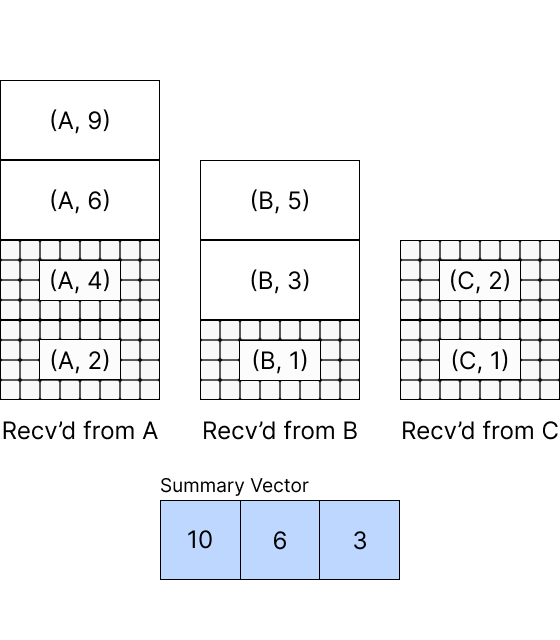
\includegraphics[width=0.6\textwidth]{images/conit/Numerical1.png}
  \caption{Figure for Example \ref{ex:conit-numerical} where
    messages with a shaded grid background represent this process' view of $\WL{C}$.}
  \label{fig:conit-numerical}
\end{figure}

\begin{example}
  \label{ex:conit-numerical}
  Figure \ref{fig:conit-numerical} depicts the role of numerical
  weight. We assume all writes apply unit weight to a single conit. If
  the lightly shaded messages represent this process' view of
  $\WL{C}$, the combined weight of the four writes estimated to be
  unseen must not exceed
  \mbox{$\epsilon^C_\textrm{num} / \left(3 - 1\right)$}.
\end{example}

\subsubsection{Order consistency}
\label{sssec:conit-order-consistency}
Recall that that the write log $\WL{P}$ is a linearly ordered
structure. Messages are initially received and applied tentatively to
$D_P$ in an uncommitted state. Eventually they will become committed
in a common global order, but the relative position of each tentative
write in the final order is not fixed. Writes applied in the wrong
order will have to be rolled back. The rolling back process may
involve application-specified logic and be associated with a cost, so
tentative writes represent a liability. The goal of ordered
consistency to is to bound this liability.

For instance, suppose an airline reservation application is used to
book individual seats for a flight. Suppose $P$ and $Q$ are two web
servers used to provide this service, and suppose both servers
independently process requests from clients to reserve a ticket for
seat \#1 at the same time. For efficiency, $P$ and $Q$ do not maintain
strict consistency, so they may both issue tickets and double-book the
seat. On the level of TSAE, the processes issue writes $w_P$ and $w_Q$
with timestamps $(P, t)$ and $(Q, t)$, respectively, and update their
local replicas to $\Dinit + w_P$ and $\Dinit + w_Q$. Eventually, $P$
and $Q$ synchronize, where the issue is discovered---the final
database state \mbox{$\Dinit + w_P + w_Q$} attempts to reserve seat
\#1 twice.\footnote{Semantically, the reader should think of the
  expression $\Dinit + w_P + w_Q$ as meaning something like, ``Reserve
  seat \#1 to $P$'s client, then issue a refund to $Q$'s client.''}
The business may decide that $P$'s ticket is valid, but the customer
who reserved a ticket from $Q$ may lose their ticket and be issued a
refund, plus a compensation fee. Thus, at the time of accepting $w_Q$
in a tentative state, the fact that $w_Q$ could be rolled back
represented a liability, and clearly one that applications may want to
bound. This is the purpose of controlling order error.

Let $\Uncommitted{P}$ represent the uncommitted messages in $\WL{P}$,
with $\Uncommitted{P}|_{\mathcal{F}}$ denoting the writes that affect
any of the conits in a set $\mathcal{F}$. Each write is $w$ is
associated with an \emph{order weight}, intended to capture the cost
of having to apply $w$ in a different order than the one it was first
applied. Let $r$ be a read access submitted to $P$ with a dependency
on conit set $\mathcal{F}$. Let $\PH_{\textrm{obs}}$ be the observed
prefix history. Now $\PH_{\textrm{obs}} \cap \PH_{\textrm{ideal}}$,
the common prefix of the observed and ideal history, represents the
longest part of $\PH_{\textrm{obs}}$ that is correct (i.e. agrees with
the ideal history). Therefore,
$\PH_{\textrm{obs}} \setminus \left(\PH_{\textrm{obs}} \cap
  \PH_{\textrm{ideal}}\right)$ represents all of the accesses that
have been applied to $P$'s local replica that will have to be rolled
back during the eventual write committment process. For purposes of
order error, we are only interested in measuring writes that affect
the conits. The order error is the combined order weight of these
writes:
\begin{definition}[Order error]
  The \emph{order error} of an access depending on a conit set
  $\mathcal{F}$ is the following sum (where $-$ denotes set difference):
  \[
    \mathsf{OrderError}\left(r, \mathcal{F}\right) \equiv \sum_{F \in \mathcal{F}} \left\{\OrderWeight\left(w, F\right) | w \in \PH_{\textrm{obs}}|_\Conits - \left(\PH_{\textrm{obs}}|_\Conits \cap
  \PH_{\textrm{ideal}}|_\Conits \right) \right\}
\]
\end{definition}

Since committed writes are globally totally ordered, the set of writes
in
$\PH_{\textrm{obs}} \setminus \left(\PH_{\textrm{obs}} \cap
  \PH_{\textrm{ideal}}\right)$ is a subset of the uncommitted
writes. Thus, we can bound the uncommitted order weight on a conit
$F$ is defined as the sum
\[ \sum_{F \in \mathcal{F}} \{\mathsf{OrdWeight}\left(w, F\right) | w \in \Uncommitted{P}|_{\mathcal{F}}\}
\]

Let $\epoe$ be the allowable upper bound of
$\OrderError\left(r,\mathcal{F}\right)$. To bound order error, it is
enough to bound the estimated value shown above. Whenever $P$ accepts
an access that, if added to $\WL{P}$, would cause the estimated order
weight to exceed $\epoe$, then $P$ must execute a write commitment
protocol to reduce the size of $\Uncommitted{P}$. This is implemented
with a \emph{pull-based} approach, as $P$ must advance its commit line
($\min_{X \in \AllProc} \left(\summary{P}{X}\right)$) far enough for
the write commitment protocol to decide the final order of enough
writes until the order error is within bounds.

\begin{figure}
  \begin{subfigure}{0.5\textwidth}
    \centering
    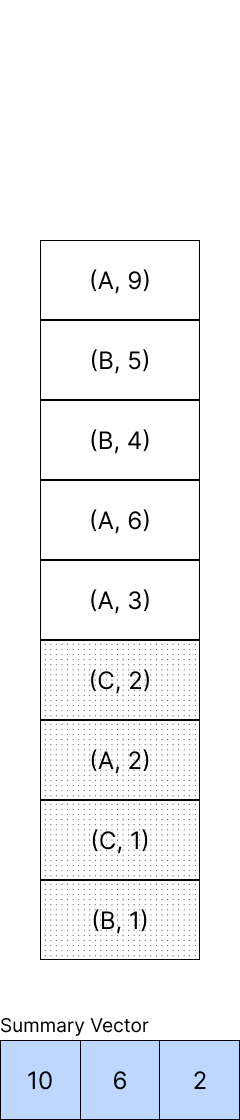
\includegraphics[width=0.5\textwidth]{images/conit/Order1.png}
    \caption{$\WL{A}$ shown with $5$ uncommitted writes}
    \label{fig:conit-order-a}
  \end{subfigure}%
  \begin{subfigure}{0.5\textwidth}
    \centering
    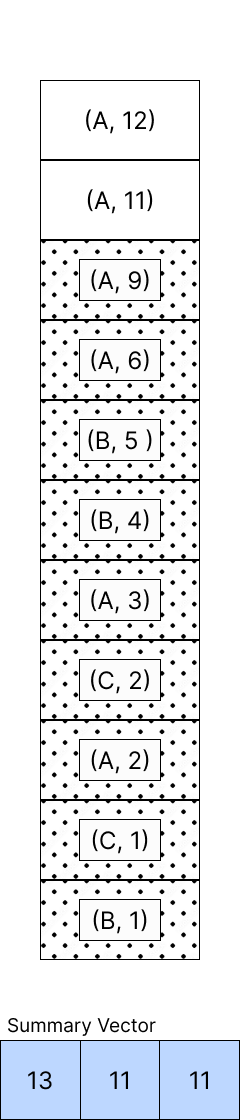
\includegraphics[width=0.5\textwidth]{images/conit/Order2.png}
    \caption{$\WL{A}$ shown at a later time}
    \label{fig:conit-order-b}
  \end{subfigure}
  \caption{Logs for Example \ref{ex:conit-order} where committed writes are drawn with a shaded and dotted background}
  \label{fig:conit-order}
\end{figure}

\begin{example}
  \label{ex:conit-order}
  Figure \ref{fig:conit-order} depicts the role of order weight. We
  assume all writes apply unit weight to a single conit. Committed
  writes are shown slightly shaded with a dotted grid pattern. In
  Figure \ref{fig:conit-order-a}, five writes are uncommitted. In
  particular, no write with timestamp greater than or equal to $3$ can
  be committed, since the minimum entry in the log, $\WL{A}{C}$, is
  only $2$.

  The next access added to $\WL{A}$ will observe an incorrect prefix
  history,
  \[\PH_{\textrm{obs}} - \left(\PH_{\textrm{obs}} \cap
      \PH_{\textrm{ideal}}\right),\] consisting of all writes after
  and including $(A, 6)$, the point at which the write log deviates
  from the ideal history (seen in Figure
  \ref{fig:conit-order-b}). This corresponds to an order error of
  $4$. Note that the message $(A, 3)$ happens to be in its ideal
  position and does not count towards the actual error, but it does
  contribute to the estimated order error of $5$, the combined weight
  of all uncommitted writes. If $5$ exceeds the allowable order error
  of the next access, the process will invoke the write commitment
  protocol, pulling updates from $B$ and $C$ to advance $A$'s summary
  vector before handling any new operation.
\end{example}

\subsubsection{Real time staleness}
\label{sssec:conit-real-time-consistency}
The \emph{real time staleness} metric allows each process $P$ to bound
the maximum amount of time between an access affecting a conit being
issued and $P$ seeing that access. Here we rely on the assumption that
$\summaryVec{P}$ stores physical timestamps from loosely synchronized
physical clocks, though this assumption can be weakened. Let $P$ have
an upper bound of $\eprt \geq 0$ on the real-time staleness of a conit
$F$. Here, $\eprt$ should be greater than the time it takes for $P$ to
engage in a typical anti-entropy session. The rule for enforcing
real-time bounds is very simple.

While handling an access with a read dependency on $F$, submitted at
time $t$, $P$ checks for each $X \in \AllProc$ whether
$|\clock{P, t} - \summary{P}{X}| < \eprt$ is true. If it is not true,
then $P$ engages in a pull-based anti-entropy session with $X$, at
which point $\summary{P}{X}$ has value $\clock{X, t'}$ for some
$t' > t$. Note that the assumption of loose synchronization implies
$\clock{X, t'} \approx \clock{P, t}$ if $t \approx t'$. This protocol
ensures that the original access, timestamped with value
$\clock{P,t}$, will observe the effect of all writes affecting $F$
with timestamps less than $\clock{P,t} - \eprt$.

A pull-based protocol may seem wasteful because $P$ may poll $X$ for
updates even if $X$ does not have any new writes. However, an approach
where $X$ pushes updates to $P$ cannot bound real-time staleness
without an upper bound on the time it takes to push messages across
the network to $P$.

If clocks are not loosely synchronized, an alternative implementation
strategy is for $P$ to maintain a vector $\vtphys{P}{}$ where
$\vtphys{P}[X]$ stores the value $\clock{P,t}$ of $P$'s clock at the
last time $P$ was on the receiving end of an anti-entropy session
directly with $X$. Then $P$ enforces consistency by ensuring that
$|\clock{P, t} - \vtphys{P}{[X]}| < \eprt$ is true before handling an
access submitted at time $t$. Since this approach only compares values
from $P$'s clock, synchronization is not required assuming $\clock{P}$
runs at a constant rate. However, this approach has the downside that,
unlike $\summary{P}{Q}$, $\vtphys{P}[Q]$ cannot be updated based on
information indirectly learned during anti-entropy with a third
party.

\subsubsection{Conit Variations and Extensions}
\label{sssec:conit-extensions}
One can imagine various ways that the conit model can be augmented
with additional capabilities. These topics are outside the scope of
this memo but offered for future consideration.

\paragraph{Dynamic bounds}
Because real-time staleness and order error are bounded by pull-based
anti-entropy sessions, it is straightforward to allow the user to
dynamically change the error bounds at each site. However, numerical
error is bounded by a push-based approach that requires every process
to be track all other processes' error bounds and cooperate to enforce
it. Therefore, dynamically tuning numerical $P$'s numerical error
bounds requires a consensus mechanism so that $P$ can inform other
processes any changes to its error bounds. However, $P$ cannot be sure
its new bounds will be respected until every process has acknowledged
the update.

Yu and Vahdat do not propose a particular mechanism for consensus. One
possible approach may be to reuse the existing message-propagating
mechanism to announce changes to error bounds, similar to Golding's
approach for handling dynamic group membership.

\paragraph{Dynamic conits}
The framework we have described above assumes the set of conits is
fixed in advance. Besides tuning bounds dynamically, we can imagine
situations where new conits need to be created on-the-fly. For
instance, data related to a new wildfire that has emerged may require
forming new conits to set consistency bounds.

Donkervliet's master's thesis \cite{dyconits} explored the subject of
dynamic conit creation in the context of massive multiplayer online
games, particularly Minecraft. In that work, new conits may be
associated with newly encountered objects in an area, and their
consistency bounds tuned as the user approaches them, exploiting a
form of locality to allocate network resources for information the
where inconsistency would most readily be perceived by the
player. Adapting their \emph{dyconits} (dynamic conits) framework to
the wide-area tactical environment may be worthwhile.

\paragraph{Interaction with the Network}
We mentioned in Section \ref{sssec:allocation-of-network-resource} our
expectation of a tighter, more complex interaction between the network
and application layers in this environment because of the need to
optimize scarce network resources for the most important
information. Because conits can quantify divergence, and therefore
indirectly the relative importance of an update, one way this might be
realized is by making the network conit-aware.

Network packets, or DTN bundles, could be specially marked as
containing database updates alongside any metadata (such as the weight
of an update to various conits) that could be used by the network for
quality-of-service purposes. Such usage may run contrary to the
conventional wisdom that networking protocols should be agnostic to
the actual content of a message, e.g. routers should be concerned only
with the data in IP packet headers but not the data contained in the
packet. This sort of atypical usage is potentially justified in our
setting because of a heightened requirement to optimize the user of
very scarce networking resources, even at the cost of blurring the
line between the network and application layers.

Modifying a network protocol to optimize a particular middleware or
application is not a lightweight task, particularly since network
drivers are often embedded into an operating system kernel or into
hardware---this makes their modification difficult or at least
fraught. We conjecture that SDN would be particularly suitable because
it is easier to modify or customize software-defined networking
protocols, so that custom hardware is not required even for extremely
specialized networking needs. The ability to design network protocols
at the level of conventional application software, rather than baking
them into hardware, might offer the flexibility to experiment with
variations of protocols.

We previously mentioned an example where a UAV or a message ferry
could be deployed dynamically to provide greater throughput in a
particular geographical area. Such a resource could be dispatched if
the application signals to a network controller that it is struggling
to enforce conit bounds in a timely manner.

Yu and Vahdat discuss quality of service as one of the features that
might itself use conits.



\section{Conclusion and Summary}
\label{sec:conclusion}

\section*{Bibliography}\label{bibliography}
\addcontentsline{toc}{section}{Bibliography}

\bibliographystyle{abbrv}
\bibliography{bibliography}
\end{document}

%%% Local Variables:
%%% mode: LaTeX
%%% TeX-master: t
%%% End:
